\documentclass[12pt]{ociamthesis}  % default square logo 
%\documentclass[12pt,beltcrest]{ociamthesis} % use old belt crest logo
%\documentclass[12pt,shieldcrest]{ociamthesis} % use older shield crest logo

%load any additional packages
\usepackage{amssymb}
\usepackage{amsmath}
\usepackage{color}
\usepackage{mathtools}
\usepackage{bbold}
\usepackage{siunitx}
\usepackage{array}
\usepackage{natbib}
\usepackage{appendix}
\usepackage{chngcntr}
\usepackage{lscape} %need this for landscape page in Chapter 4

\usepackage{etoolbox}%need for subappendices
\bibliographystyle{plainnat} 
 \renewcommand{\familydefault}{\sfdefault}
\setcounter{secnumdepth}{2}
\setcounter{tocdepth}{2}

%this baselineskip gives sufficient line spacing for an examiner to easily
%markup the thesis with comments
\baselineskip=18pt plus1pt

%set the number of sectioning levels that get number and appear in the contents

%\begin{romanpages}          % start roman page numbering
%\listoffigures              % generate and include a list of figures
%\end{romanpages}            % end roman page numbering

%\renewcommand{\thesubsection}{\Alph{subsection}} %for making appendices have letters


\title{Droplet Transport by Bendotaxis}   %your thesis title,
         %note \\[1ex] is a line break in the title

\author{Alexander Bradley}             %your name
\college{Lincoln College}  %your college

\renewcommand{\submittedtext}{Submitted for the degree of}
\degree{Doctor of Philosophy}     %the degree
\degreedate{Trinity 2020}         %the degree date

%end the preamble and start the document
\begin{document}

%this baselineskip gives sufficient line spacing for an examiner to easily
%markup the thesis with comments
\baselineskip=18pt plus1pt

%set the number of sectioning levels that get number and appear in the contents
\setcounter{secnumdepth}{2}
\setcounter{tocdepth}{1}

%need below for correctly including sub-appendices
%\AtBeginEnvironment{subappendices}{%
%\section*{Appendix}
%\addcontentsline{toc}{Section}{Appendices}
%\counterwithin{figure}{section}
%\counterwithin{table}{section}
%}
% End of subappendices environment
%\AtEndEnvironment{subappendices}{%
%\counterwithout{figure}{section}
%\counterwithout{table}{section}
%}

\maketitle                  % create a title page from the preamble info
\begin{preface}
The research described in this thesis was performed in the Mathematical Institute at the University of Oxford between October 2016 and May 2020, and was supervised by Professor Dominic Vella and Professor Ian J. Hewitt.

This thesis describes my own work, including the experiments described in Chapter 3. I am grateful to Finn Box for his help developing the experimental protocol and prototype experiments on the system. 

The results presented in this thesis are original, apart from the discussion in \S6.6.1 which constitutes review material, and where reference is made to the work of others. No part of the thesis has been submitted previously for a degree of the University or elsewhere.

At the time of writing, one paper based on the work presented in this thesis has been published in Physical Review Letters, co-authored with F. Box, I.J. Hewitt and D. Vella~\citep{Bradley2019PRL}. This paper is based on the mathematical modelling of bendotaxis presented in Chapter 2 and accompanying experiments presented in Chapter 3.
\end{preface}        % include a dedication.tex file
\begin{acknowledgements}
I would like to thank my supervisors Ian Hewitt and Dominic Vella for their guidance and support, both academically and personally, throughout my dPhil. Without their patience, generosity and insight, this project would not have been possible.

Thanks also to my peers within OCIAM and Oxford Mathematics. Amongst this special community, I'd like to say special thanks to my office mates, Matt Butler and Michael Coughlan, for helpful suggestions and thoughtful answers to (often stupid) questions; to Finn Box for his patience and assistance with experiments; to the squishy club members for fostering a constructive and non-judgemental environment for discussion and presentation practice; and to Andreas M\"{u}nch, Peter Howell, and Ian Griffiths for their helpful comments on earlier versions of chapters. 

Finally, thanks to my family for their unwavering support and encouragement and to Rebecca Smith, without whom this thesis would not have been possible. 
\end{acknowledgements}  % include an acknowledgements.tex file
\begin{abstract}
In this thesis, we study bendotaxis -- a novel, passive droplet transport mechanism driven by the coupling between capillary pressure within the droplet and bending deformations of the channel confining it. This mechanism is inspired by observations of the legs of Gerris Regimis, which are covered in setae rendering them superhydrophobic; the setae deform by bending in response to the capillary pressure of vapour droplets as they condense between setae, resulting in their dynamic expulsion, and thus helping to maintain a superhydrophobic leg.

In the first half of this thesis, we focus on two dimensional scenarios to isolate the underlying competition between bending and capillarity. In this setup, the direction of droplet transport is, surprisingly, always the same, regardless of the wettability of the channel. We use a combination of experiments at a macroscopic scale and a simple mathematical model to study this motion, focusing in particular on the time scale associated with the motion. We make observations that may inform the design of superhydrophobic surfaces exploiting bendotaxis for anti-fogging and also investigate two physical effects -- contact angle hysteresis and droplet self-trapping -- which can impede droplet transport by bendotaxis. 

In the second half of this thesis, we focus on the influence of channel geometry on droplet transport by bendotaxis.  Further motivation is provided by experiments in which a regular, periodic pattern emerges as liquid droplets are condensed into deformable microchannels and move in a manner similar to bendotaxis. We hypothesize that this wavelength selection is the result of a novel instability, reminiscent of the Rayleigh-Plateau instability but mediated by channel elasticity. By developing and analyzing a mathematical model of a system susceptible to this instability, we study its characteristic behaviour and the consider the effect of adding liquid to the channel as the instability develops.

Finally, we consider how collaborative effects of droplet transport by bendotaxis in neighbouring channels may lead to clustering. We first develop a mathematical model for an array of droplet-channel systems, each of which would undergo bendotaxis in isolation, and, using this, identify two distinct regimes for the cluster sizes in the limits of weak and strong surface tension, which are then derived analytically using asymptotic methods. 
\end{abstract}          % include the abstract

\begin{romanpages}          % start roman page numbering
\tableofcontents            % generate and include a table of contents
%\listoffigures              % generate and include a list of figures
\end{romanpages}            % end roman page numbering

%new commands not contained in sub files
\newcommand\abceqn[2]{\refstepcounter{equation}
     \[
     \label{#1}
     #2
     \eqno{\text{(\theequation)}\text{a,b,c}}
     \]
}


\graphicspath{{./Sections/Chapter1_intro/figures/}}
\chapter{Introduction}
\section{A primer on superhydrophobic surfaces}\label{S:Ch1:superhydrophobic}
This thesis is concerned with droplet transport in response to flexible boundaries. However, the motivation for studying this comes from manufacturing superhydrophobic surfaces that are not compromised by the condensation of vapour. This section provides a brief background to the rapidly expanding field of superhydrophobic surfaces. A more detailed overview can be found in the review paper by~\cite{Simpson2015RepProgPhys}, for example.

\begin{figure}[t]
\centering
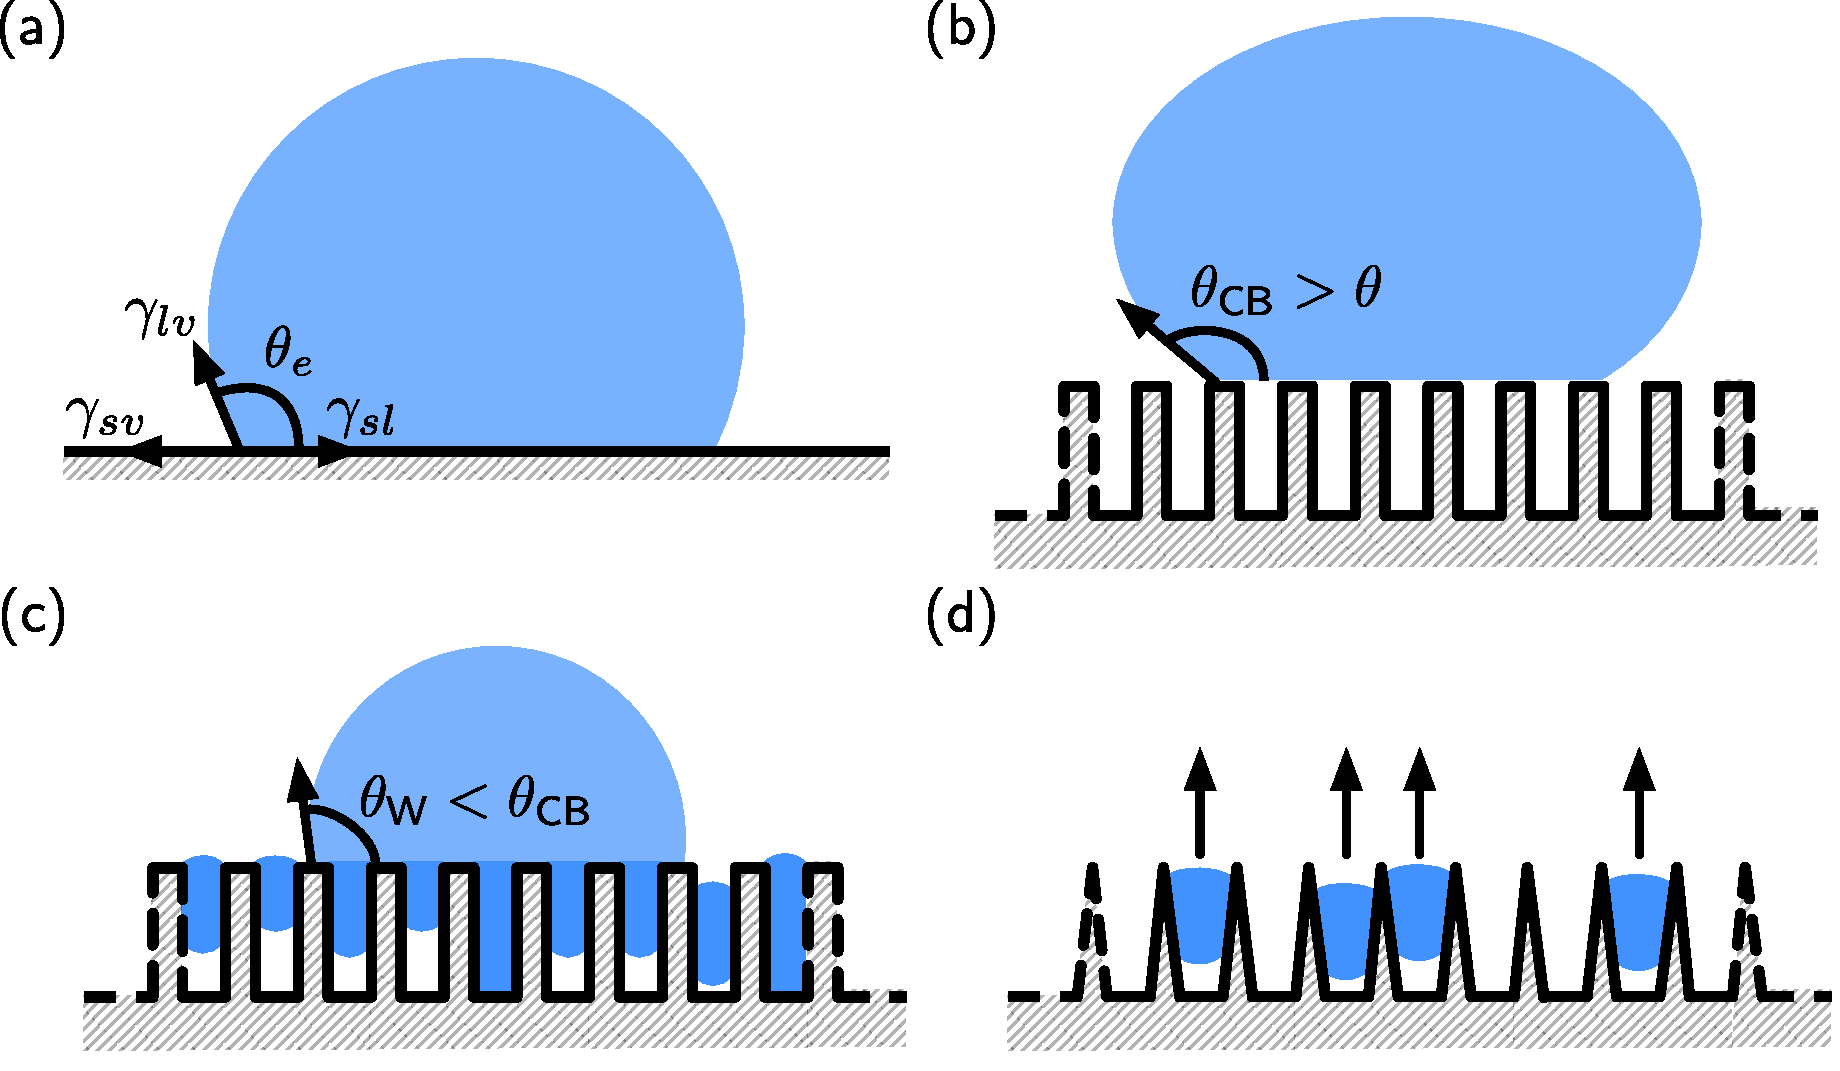
\includegraphics[scale=0.42]{Texturing}
\caption{(a) A sessile droplet on a solid surface takes the macroscopic contact angle $\theta_e$ that results in a balance between the  liquid-vapour, solid-liquid, and solid-vapour interfacial energies $\gamma_{lv}$, $\gamma_{sl}$, and $\gamma_{sv}$, respectively, according to Young's equation~\eqref{E:Ch1:Young}. (b) A droplet perched on top of topographical structures in a Cassie-Baxter state makes a macroscopic contact angle greater than that specified by Young's equation. (c) If the droplet (light blue) contacts a surface whose topographical features contain condensed droplets (dark blue), it is in a Wenzel state, characterized by a lower macroscopic contact angle (compared to a Cassie-Baxter state) and reduced mobility. (d) If the topographical features are conically shaped, fewer droplets condensate between them, and those that do may be driven out of the channels that exist between features.}\label{fig:Ch1:Textured}
\end{figure}



Informally, superhydrophobic surfaces are characterized by the observation that water droplets placed on them take almost ball-like shapes, and roll or slide off easily. As they do so, droplets may entrain surface contaminants, effectively cleaning the surface~\citep{Blossey2003Nature}. For this reason, superhydrophobic surfaces can be considered a class of `self-cleaning' surfaces~\citep{Liu2012AnnRevMaterSci}. A  familiar natural example of a superhydrophobic self-cleaning surface is the leaf of the lotus plant (\textit{Nelumbo nucifera})~\citep{Barthlott1997Planta}; indeed, self cleaning surfaces are often said to exhibit `the lotus effect'~\citep{Marmur2004Langmuir}. Nevertheless, superhydrophobic surfaces have a wide range of applications beyond self-cleaning, including corrosion resistance~\citep{Liu2011Nanoscale}, drag reduction~\citep{McHale2010SoftMatter}, and anti-icing~\citep{Meuler2010ACSnano}.

%but they're more useful than just as self-cleaning  surfaces --.> artificial examples

%A surface is rendered superhydrophobic using a combination of surface texturing and chemistry
% \red{what happens on a flat surface, and flat cannot be superhydrophobic}
\subsubsection{Contact angles on superhydrophobic surfaces}
The heuristic notion of superhydrophobicity introduced above is made more formal by introducing the contact angle $\theta$: the macroscopic angle that a sessile droplet makes with a surface; a surface is superhydrophobic if it has a contact angle $\theta > 150\si{\degree}$~\citep{Ma2006CurrOpCollSci}.

If the surface is homogeneous and smooth, and the droplet is in equilibrium, the contact angle is the Young angle $\theta_e$, which is set by the material properties via Young's equation~\citep{Young1805PhilosTrans, deGennes1985RevModPhy},
 \begin{equation}\label{E:Ch1:Young}
 \cos \theta_e = \frac{\gamma_{sv} - \gamma_{sl}}{\gamma_{lv}}.
 \end{equation}
Here $\gamma_{sv}, \gamma_{sl}$, and $\gamma_{lv}$ are the interfacial energies at the solid-vapour, solid-liquid, and liquid-vapour interfaces (Figure~\ref{fig:Ch1:Textured}(a)).

In reality, however, surfaces are heterogenous, and droplets are not always in equilibrium. In these cases, the contact angle is not unique: if the droplet's contact line (the line of contact between solid and liquid) is stationary, it's contact angle can take any value between an advancing angle, $\theta_a$, and a receding angle, $\theta_r$. In addition, if the contact line is advancing, the contact angle takes this advancing angle and if the contact line is receding, the contact angle takes the receding angle. The contact angle hysteresis is defined as the difference between these angles, $\theta_a - \theta_r$. Superhydrophobic surfaces typically exhibit low contact angle hysteresis (superhydrophobic surfaces with a contact angle hysteresis less than $\si{10\degree}$ are said to be super-repellent~\citep{Attinger2016Nanoscale}).

\subsubsection{Making superhydrophobic surfaces}
The maximum Young angle that has been achieved using known materials and a water droplet is approximately $ 120\si{\degree}$~\citep{Blow2010Langmuir}. Nevertheless, many examples of surfaces with contact angles approaching 180$\si{\degree}$ exist. Such large contact angles can be achieved by introducing topographical features to the surface~\citep{Bico2001EPL}: droplets are able to perch on top of features in a so called Cassie-Baxter state~\citep{Cassie1944TransFaraday,Cassie1948FaradayDiscuss}; their macroscopic contact angle is increased, compared to a flat surface, because much of the solid-liquid contact has replaced by liquid-air contact (Figure~\ref{fig:Ch1:Textured}(b)). Explicitly, the contact angle of a droplet in a Cassie-Baxter state, $\theta_{\text{CB}}$, satisfies~\citep{Lafuma2003NatureMat}
\begin{equation}
\cos  \theta_{\text{CB}} = \phi \cos \theta_e - (1-\phi)
\end{equation}
where $\phi$ is the fraction of the footprint of the droplet in contact with the solid surface. The lotus leaf, for example, employs a hierarchical structure of papillose epidermal cells~\citep{Neinhuis1997AnnBot} to increase
surface roughness, resulting in contact angles above 160$\si{\degree}$~\citep{Barthlott1997Planta}. By modifying the surface topography, surfaces demonstrating contact angles all the way up to 180\si{\degree}, the maximum possible, have been manufactured~\citep{Bico1999EPL, Quere2005RepProgPhys}.

\subsubsection{Textured superhydrophobic surfaces fog up}
One major limitation of using texturing to create superhydrophobic surfaces is their tendency to ‘get wet’ when exposed to foggy or humid environments -- droplets of a size comparable to the scale of the texturing nucleate and grow within it, destroying the Cassie-Baxter state~\citep{Dorrer2007Langmuir,Varanasi2009APL}. Macroscopic droplets subsequently deposited on the surface come into contact with existing liquid bridges embedded within the texturing (Figure~\ref{fig:Ch1:Textured}(c)), thereby becoming a `Wenzel' state~\citep{Wenzel1949JPhysChem}. The contact angle $\theta_{\text{W}}$ of a droplet in a Wenzel state satisfies
\begin{equation}
\cos \theta_{\text{W}} = r\cos \theta_e,
\end{equation}
where $r>1$ is the ratio of the actual surface area to apparent surface area of the texturing. A droplet in a Wenzel state has significantly reduced mobility, compared to a Cassie-Baxter state -- the contact angle is lower, and the droplet may pin strongly on the topographical features, leading to a significantly increased contact angle hysteresis. Lotus leaves, for example, have been observed to experience an increase in their roll off angle (the angle that the surface must be rotated to in order to initiate rolling, a measure of contact angle hysteresis) from $\lesssim$~\si{5~\si{\degree}} to above 70\si{\degree} when droplets are condensed, rather than deposited, onto their surface~\citep{Cheng2005aAPL,Cheng2005bAPL}.

Of course, nature experiences this same problem and has found at least one solution: by tailoring the shape of the topographical structures, fog build-up can be reduced. For example, the texturing on  the superhydrophobic wings of some cicada~\citep{Wisdom2013PNAS} and butterflies~\citep{Chen2018PLOSone} features conical structures (shown schematically in Figure~\ref{fig:Ch1:Textured}(d)). These structures are believed to reduce the total  number of nucleating droplets because there is less room for condensation to occur near the base of the cones~\citep{Xu2016RSCadv}.  In addition, droplets that bridge between two neighbouring cones may be spontaneously propelled towards their tips (i.e.~away from the surface). Droplets can be removed from the tips by mechanical actuation or by spontaneous jumping after coalescing with an adjacent droplet~\citep{Boreyko2009PRL, Boreyko2010PhysFlu} (coalescing with another droplet releases surface energy, which is converted into kinetic energy). By mimicking these natural structures,  artificial superhydrophobic surfaces with conically shaped protrusions have been shown to perform significantly better in foggy conditions than superhydrophobic surfaces with cylindrical features~\citep{Mouterde2017NatMater}.

The above example of antifogging of a superhydrophobic surface is facilitated by spontaneous droplet transport in response to the geometric gradient that arises when a droplet bridges two neighbouring cones. Such motion driven by geometric gradients is  one of a number of mechanisms for transporting droplets. We discuss these mechanisms in more detail next.

\section{Droplet transport}
%Moving small droplets: dominated by surface tension.
Liquid droplets experience body forces (gravity) and surface forces (surface tension). If a droplet has a typical length scale $L$, then body forces scale with $L^3$, while surface forces scale with $L^2$~\citep{deGennes2004}; this means that surface forces dominate the behaviour of sufficiently small droplets. The length scale below which surface tension dominates over gravity is the capillary length, $\ell_c = (\Delta \rho g/\gamma)^{1/2}$, where $\rho$ is the liquid density (assuming a negligible ambient density), $g$ is gravitation acceleration and $\gamma$ the interfacial tension coefficient~\citep{deGennes2004}. In this thesis, we are concerned with droplets of characteristic size below the capillary length.


%why do we care about moving small droplets
As we saw in \S\ref{S:Ch1:superhydrophobic}, control and transport of liquid droplets smaller than the capillary length is important in preventing fog build-up within the topographical features on superhydrophobic surfaces. More broadly, the transport of small droplets is critical in a wide range of applications including diagnostics~\citep{Yager2006Nature}, fog harvesting~\citep{Andrews2011Langmuir}, microfabrication~\citep{Srinivasarao2001Science}, and droplet-based microfluidics~\citep{Squires2005RevModPhys}.

%so if we want to move small droplets, we need to think about surface tension. we can either change the interfacial tension --> i.e. marangoni, or we can create a wettability gradient to create curvature differences on either side of the droplet and hence laplace pressure difference = flow. You can do this by making the contact angle vary across the droplet (e.g. chemical composition, nano-structuring gradients) or using geometry.

Liquid motion within a droplet is driven by gradients in the liquid pressure $p$. Locally, the droplet pressure (its Laplace pressure) is set by the surface tension $\gamma$ and interfacial curvature $\kappa$ according to the Young-Laplace equation $p = \gamma \kappa$~\citep{Laplace1799,Young1805PhilosTrans}. There are, therefore, two ways to generate droplet motion~\citep{Scriven1960Nature}: by creating gradients in surface tension, or by creating gradients in interfacial curvature.

Local variations in the surface tension, thereby generating a Marangoni flow within the droplet (towards regions of lower surface tension) exert a hydrodynamic force on the adjacent surface; the equal and opposite force applied by the surface propels the droplet along it.  Gradients in surface tension, or rather the associated Marangoni flow, can be created in droplets in a variety of ways including by varying the temperature across them (often called thermocapillarity)~\citep{Brzoska1993Langmuir, Pratap2008Langmuir}, by differential evaporation leading to differences in composition~\citep{Thomson1855}, by tailoring the surface chemistry~\citep{COTTINGTON1964, John2005EPJE}, and by using electrochemical effects~\citep{Gallardo1999Science}.


The second route to transporting small droplets is to create a gradient in the droplet's interfacial curvature. One way to do so is to vary the local contact angle; techniques such as electrowetting~\citep{Lippmann1875, Mugele2005JPhysCond}, variations in surface local topography~\citep{Shastry2006Langmuir}, surface chemistry~\citep{DosSantos1995PRL,Chaudhury1992Science,Daniel2001Science}, and surface photoirradiation~\citep{Ichimura2000Science} have all been successfully exploited to vary the local contact angle of, and thus transport, droplets.

Gradients in interfacial curvature can also be induced by the geometry of the adjacent surface. This method of droplet transport can be traced back three-centuries to Hauksbee~\citep{Hauksbee1710iii}, who observed that a droplet of oil between two non-parallel plates would  ``immediately move towards the touching side of the plane''. Droplet transport in similar tapered channels (wedges) has been studied in detail in more recent years by~\cite{Renvoise2009EPL} and~\cite{Reyssat2014JFM} and the mechanism is well understood: provided that the droplet wets (or has an affinity to) the walls of the channel, the negative interfacial curvature, whose magnitude is inversely proportional  to the local thickness of the wedge, is smaller (it is more negative) on the side of the droplet closest to the apex. The droplet is therefore `sucked' into the wedge. If, on the other hand, the droplet does not wet the channel walls, then the (positive) interfacial curvature is smaller at on the side furthest from the tip, where the channel is widest; non-wetting droplets are therefore squeezed out of the vertex. Crucially, we note that droplet motion in tapered channels is wettability-dependent -- wetting and non-wetting droplets move in opposite directions.

A similar mechanism is responsible for droplet propulsion from within a conically textured surface (Figure~\ref{fig:Ch1:Textured}(d)) -- the surface of the cones are themselves hydrophobic, so the droplets are pushed towards the weaker confinement at the top of the cones. Note, however, that if nucleating droplets consisting of a \textit{wetting} liquid were to bridge between two cones, the droplets would be driven in the opposite direction towards the base of the cones, rather than expelled, to the detriment of the surface's superhydrophobicity.

Droplet motion induced by geometric gradients can also be achieved without bridging; recent studies by \cite{Lv2014PRL} and~\cite{McCarthy2019SoftMatter} have described the dynamic behaviour of droplets on solid surfaces of non-constant curvature, or `curvotaxis'. In this case, droplets move indefinitely towards the region of lowest curvature if the surface curvature is positive, and vice versa for negative curvature. (This scenario is somewhat different for configurations in which the droplet wraps completely around the surface, in which case equilibrium configurations are possible~\citep{Lorenceau1999JFM, Michielsen2011Langmuir}). In contrast to the confined case, this phenomenon -- often referred to as `curvotaxis' -- is independent of wettability. Both curvotaxis and droplet motion in tapered channels are, however, passive -- they do not require external energy input -- and spontaneous -- there is, in principle,  no energy barrier to be overcome before movement is initiated (in practice, the surface will have some contact angle hysteresis that must be overcome).

In the examples above, the geometry that drives motion is fixed and independent of the droplet's presence. Recently, a new class of scenarios has emerged in which the substrate geometry is responsive to the droplet's pressure, for example via deformable boundaries. In this case, additional droplet  transport mechanisms become possible. For example,~\cite{Style2013PNAS} demonstrated that droplets placed on a deep, soft substrate move in response to gradients in the stiffness of the underlying substrate. This mechanism, named durotaxis for its superficial similarity to cell durotaxis~\citep{Lo2000Biophys}, has recently been shown to be wettability dependent~\citep{Bueno2018SoftMatter}. In addition, numerical simulations have suggested that droplets can move spontaneously in response to gradients in strain of the underlying substrate (`tensotaxis')~\citep{Bueno2017EML}. Moreover, it has recently been demonstrated that droplets on a deformable substrate can mutually attract~\citep{Karpitschka2016PNAS} in a process reminiscent of the Cheerios effect~\citep{Vella2005AJP}.

Bendotaxis, the subject of this thesis, falls into this latter class of droplet motion mechanisms. It is a passive droplet transport mechanism that relies on the bending of a channel confining the droplet in response to the droplet's capillary pressure.

\section{Bendo-capillarity}
The interaction between bending of slender objects and capillarity, sometimes referred to as bendo-capillarity~\citep{Style2017AnnRevCondMatPhs}, falls under the larger umbrella of elasto-capillarity, in which capillarity deforms elastic solids~\citep{Bico2018AnnRevFluidMech}. In bendo-capillary interactions, the surface tension $\gamma$ of an interface acts to minimize its the interfacial area, whilst the bending stiffness $B$ of the slender object tends to resist deformation.

The length scale on which bending and capillarity interact can be seen on dimensional grounds to be $\ell_{bc} = \sqrt{B/\gamma}$, the bendo-capillary length. To elucidate this length scale, we consider a thin, flexible, rectangular sheet of length $L$, width $w$, and bending stiffness $B$, that is coated in a thin layer of liquid whose surface tension is $\gamma$. If this sheet is brought into contact with a solid cylinder of radius $R$, then it has two options: to either remain flat, or to spontaneously wrap around the cylinder. Wrapping around the cylinder would release a surface energy scaling with $\gamma wL$, but would incur a bending energy scaling with $BwL/R^2$; the sheet will spontaneously wrap the cylinder if $R \gtrsim \ell_{bc} = \sqrt{B/\gamma}$, the bendo-capillary length. Heuristically, objects with a length scale larger than bendo-capillary length experience large deformations under capillary forces~\citep{Roman2010JPhysCond}, as this example demonstrates.

If the thickness of the sheet in the previous example is $b$, then its bending stiffness $B \sim b^3$~\citep{Timoshenko1959} and thus the bendo-capillary length $\ell_{bc} \sim b^{3/2}$. Therefore, if the length scales of the system are scaled by a factor $\mu$, the bendo-capillary length is scaled down by a factor $\mu^{3/2}$. This demonstrates why smaller systems are more likely to be susceptible to bendo-capillary phenomena. On the nano-scale, for example,  bendo-capillarity can be exploited for the self-assembly of carbon nanotube arrays~\citep{DeVolder2013Angewandte} and, on the micro-scale, surface tension induced aggregation (and subsequent collapse) of arrays of micro-pillars can be used to trap colloids~\citep{Pokroy2009Science}.

Bendo-capillarity is, however, also responsible for a diverse range of phenomena on macroscopic scales, such as the coalescence of wet hair~\citep{Bico2004Nature, Duprat2012Nature}, the fluid-like behaviour of a spider's web in compression~\citep{Elettro2016PNAS}, and capillary origami~\citep{Py2007PRL}.


%l >> l_{ec} -> strong deformations. l_ec scales with h^{3/2} so smaller object typically experience effects e.g. ...
%but also macroscopic effects such as....



\section{What is bendotaxis?}
  \subsection{Bio-inspiration from the Gerris Regimis}
  \begin{figure}[t]
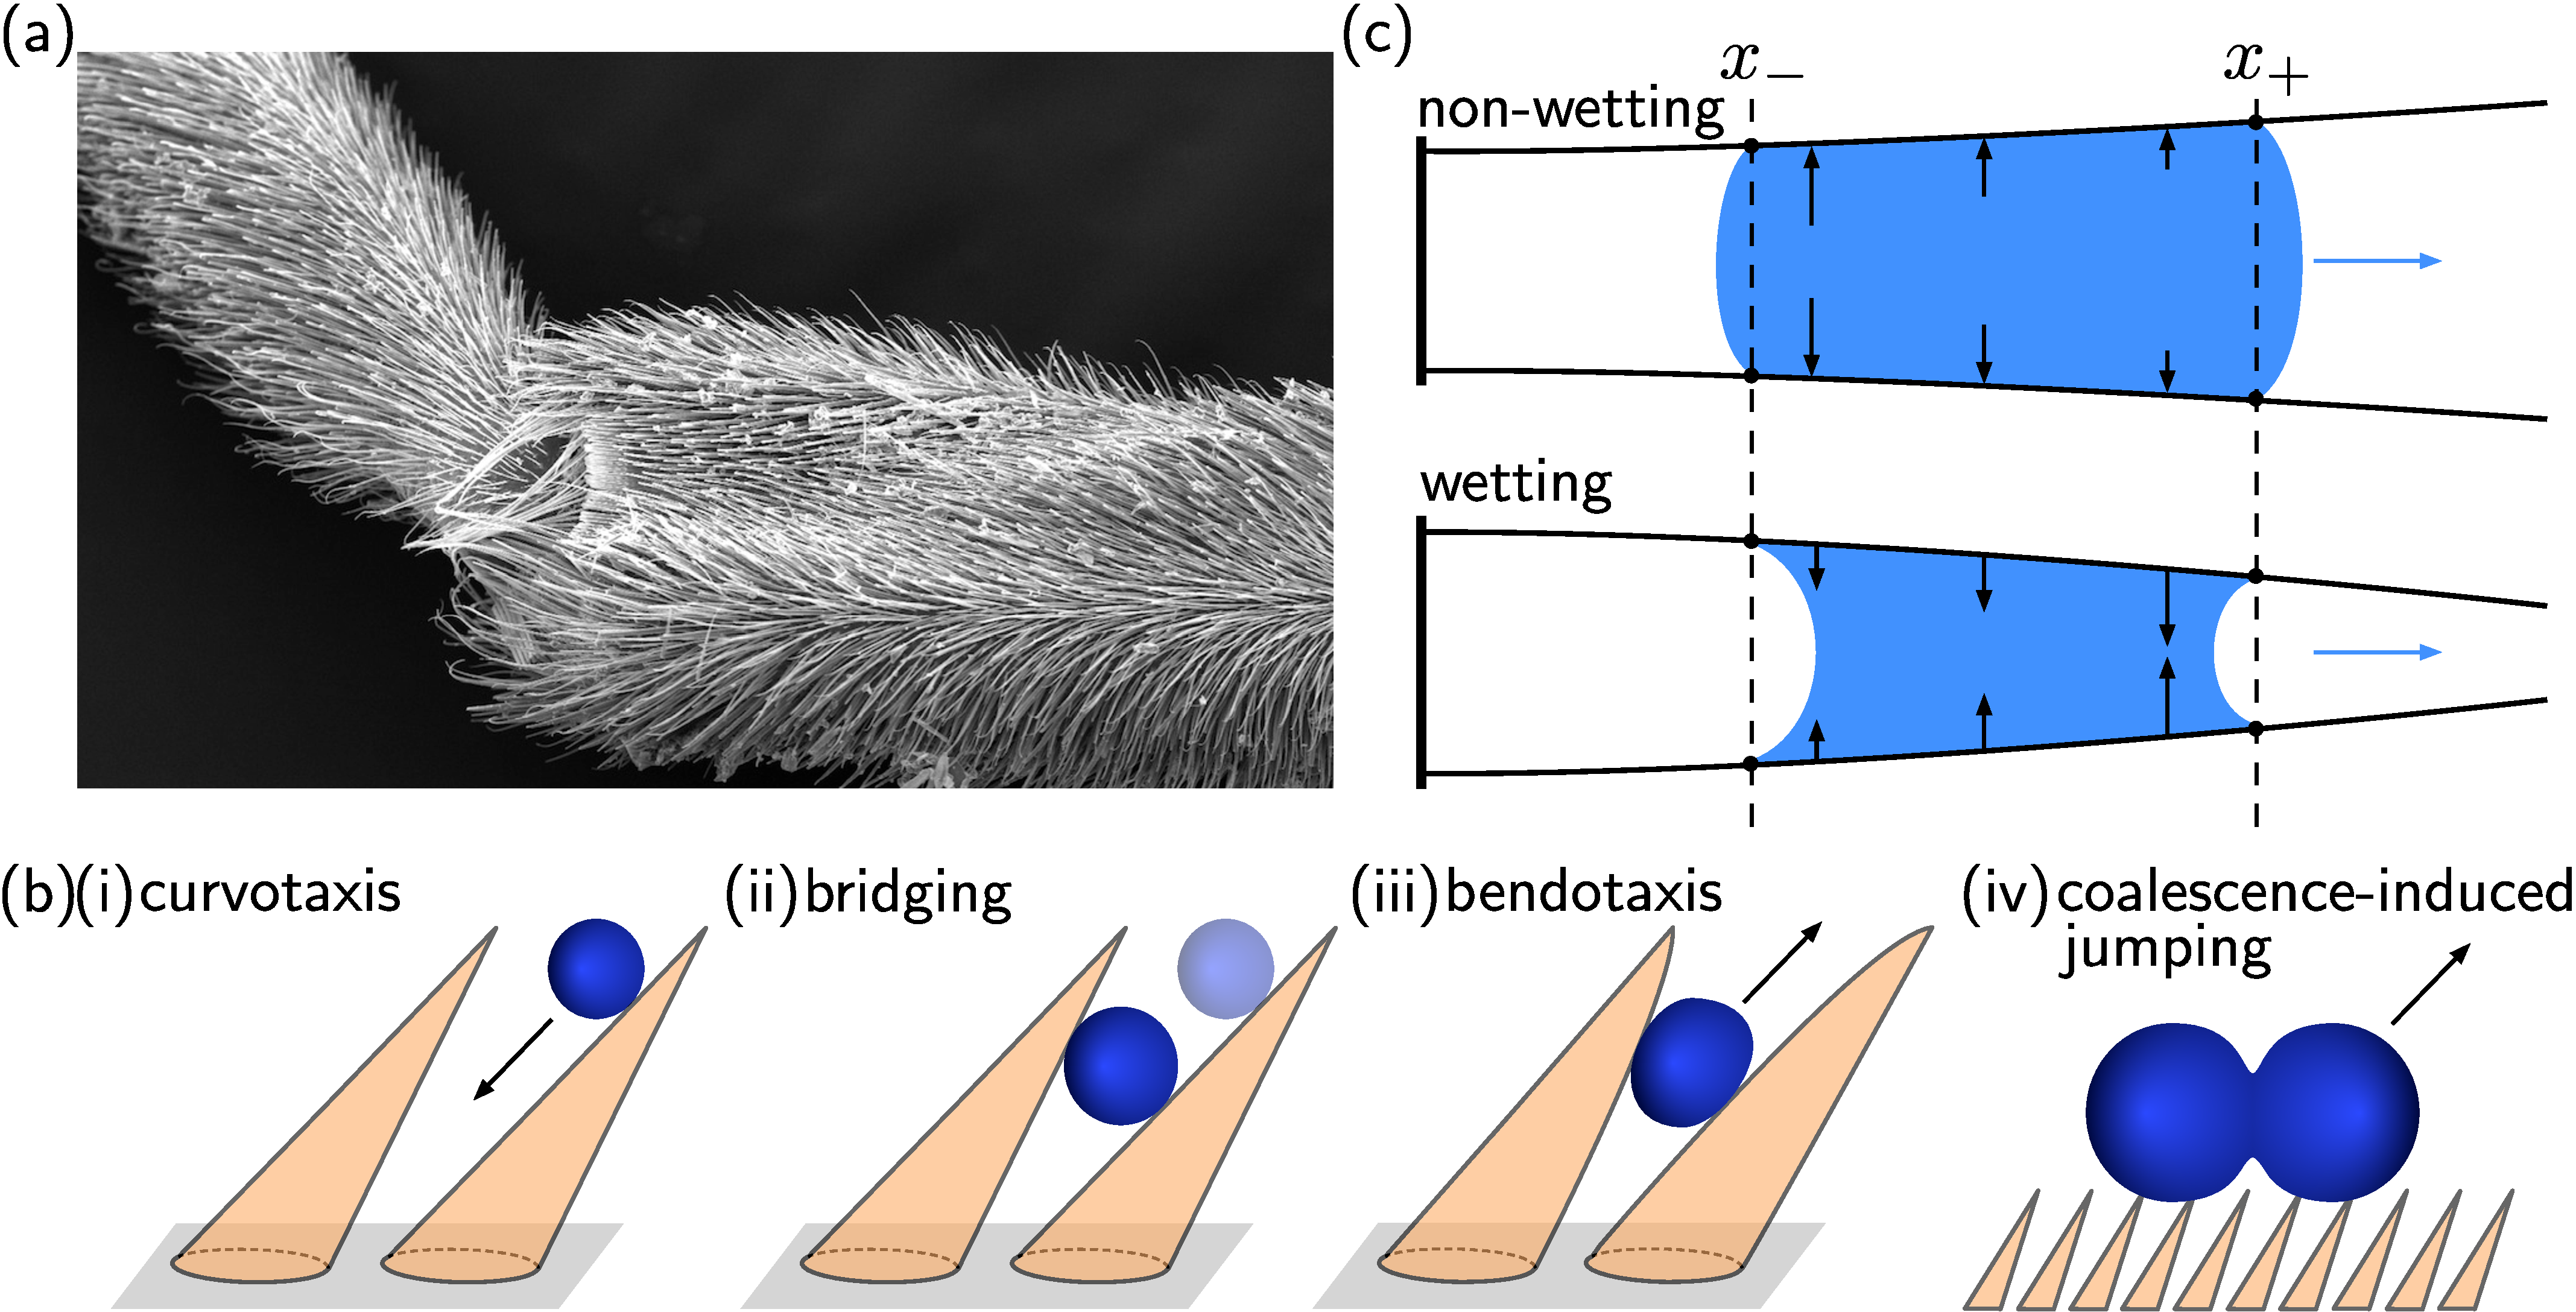
\includegraphics[width = \textwidth]{wang_schematic}
\caption{(a) Electron microscope image of a portion of the setae covering a leg of a \textit{Gerris Regimis} (or Water Strider). Collectively, the setae are responsible for the macroscopic superhydrophobicity of the leg. Image used with permission from Corinne Sommi/Swathmore College. (b) Schematic diagram of droplet removal from a channel between the setae on the leg of a water strider~\citep[after][]{Wang2015PNAS}. (i) The droplet moves along a conical seta to the narrower end of the channel via curvotaxis before (ii) contacting a neighbouring seta, all the while growing in size (via condensation). (iii) The droplet is expelled from the channel via bendotaxis (see main text), and it can subsequently be removed from the surface (iv) by coalescing with another droplet, for example. (c) Schematic diagrams explain the mechanism behind bendotaxis for non-wetting (top) and wetting (bottom) droplets. Black arrows indicate (schematically) the sign and magnitude of the Laplace pressure within the drop; blue arrows show the direction of decreasing pressure and hence droplet motion.}\label{fig:Ch1:StriderMechanism}
\end{figure}


Our inspiration for studying bendotaxis comes from recent observations of the legs of the \textit{Gerris Regimis} (commonly referred to as a Water Strider, or Pond Skater) by~\cite{Wang2015PNAS}. Water strider legs are covered in an array of conically shaped hairs (Figure~\ref{fig:Ch1:StriderMechanism}(a)), or setae. Collectively, the setae are responsible for the leg's superhydrophobicity by maintaining a Cassie-Baxter state~\citep{Gao2004Nature, Bush2006AnnRevFluidMech}. Superhydrophobicity is in turn important in reducing the energy required by the Water Strider to jump at the interface~\citep{Lee2009JFM}.

\cite{Wang2015PNAS} showed that the geometry and flexibility of the setae prevent the superhydrophobic leg from losing its water repellancy in the high humidity conditions in which the Water Strider dwells (where condensation of droplets would be an issue). As described by~\cite{Wang2015PNAS}, condensed droplets are removed from the setae in a three part process that is shown schematically in Figure~\ref{fig:Ch1:StriderMechanism}(b): firstly, a droplet of condensed water contacts a single seta and moves towards its base via curvotaxis. This phase ends with the droplet also contacting a neighbouring seta, forming a capillary bridge and effectively confining itself. The positive Laplace pressure of the droplet (water is non-wetting on the setae) then deforms this `channel' outwards, creating a geometric gradient that propels the non-wetting droplet towards regions of weaker confinement; this propulsion in response to droplet-induced channel deformations is caused by bending and hence we refer to it as bendotaxis.  Once the droplet has reached the tip, it can be removed (for example, by coalescence-induced jumping, as discussed in \S\ref{S:Ch1:superhydrophobic}).

%
%\blue{also a hat tip to Otten 2004 and Bernandino 2010 who argued about whether the flexiblity of the hairs on the Lady mantle aids with superhydrophobicity: could flexbility also help in another way?}


\subsection{Bendotaxis mechanism}
The geometry of a capillary bridge between conical setae is complicated. Moreover, the tapered channel formed by the conical fibres would expel the droplet, even in the absence of bending deformation. Therefore, to understand the mechanism of bendotaxis, and to isolate the role of bending alone, we consider the simplified scenario shown in Figure~\ref{fig:Ch1:StriderMechanism}(c): two, initially parallel, bendable walls are clamped at one end and free at the other. These two walls together form a two-dimensional channel.

If a wetting droplet is introduced between the walls, the interfacial curvature is negative at both ends of the droplet and the associated negative Laplace pressure deflects the walls inward (Figure~\ref{fig:Ch1:StriderMechanism}(c)).   The anisotropic boundary conditions (clamping at one end, free at the other) result in a channel that is effectively stiffer closer to the clamped end -- the same force applied closer to the clamped end results in a smaller deformation. As a result of this anisotropy, the channel deformation is larger at the meniscus closer to the free end (denoted $x_+$) than at the meniscus closer to the clamped end (denoted $x_-$). The pressure is therefore smaller (it is `more negative') at $x_+$ than at $x_-$, and the resulting pressure gradient drives the droplet towards the free end. Provided the contact angles remain the same and the walls do not touch, this motion will continue until the droplet reaches the free end.

If, however, a non-wetting droplet is introduced between the walls (as is the case in the setae of the water strider~\citep{Wang2015PNAS}), the Laplace pressure within the droplet is positive, pushing the walls away from one another (Figure~\ref{fig:Ch1:StriderMechanism}(c)). Again, however,  the resulting pressure gradient is negative, driving the droplet towards the free end. This argument suggest that  bendotaxis is wettability independent, the direction of motion is universal. (This thought experiment also clarifies the name bendotaxis: without channel flexibility, the pressure within the droplet would be constant and the droplet would be stationary. The droplet itself generates the tapering that leads to its motion.)

We can also view bendotaxis from an energetic perspective in this simple geometry. In the wetting case, the droplet would like to advance because the additional inwards deformation that results from this (the pressure applies at a distance further from the clamped end) will increase the length over which the droplet wets the channel (by conservation of droplet volume). Of course, this additional deformation incurs a bending energy penalty, but we shall see that, provided the channel walls do not touch, this penalty is not large enough to discourage the droplet from advancing. Similarly, in the non-wetting case, the outwards deformation that would result from the droplet's advance would lead to wetting over a shorter length, which is again energetically favourable.

It is the wettability-independence that makes it appealing to exploit bendotaxis in textured superhydrophobic surfaces: both wetting and non-wetting droplets would be spontaneously propelled towards the free end of the channel (i.e.~away from the surface, which would naturally correspond to the clamped end); this is in contrast to the rigid conically textured surfaces, in which only non-wetting droplets that bridge between cones are propelled away from the surface.

\subsection{Proof of concept}
\begin{figure}[t]
\centering
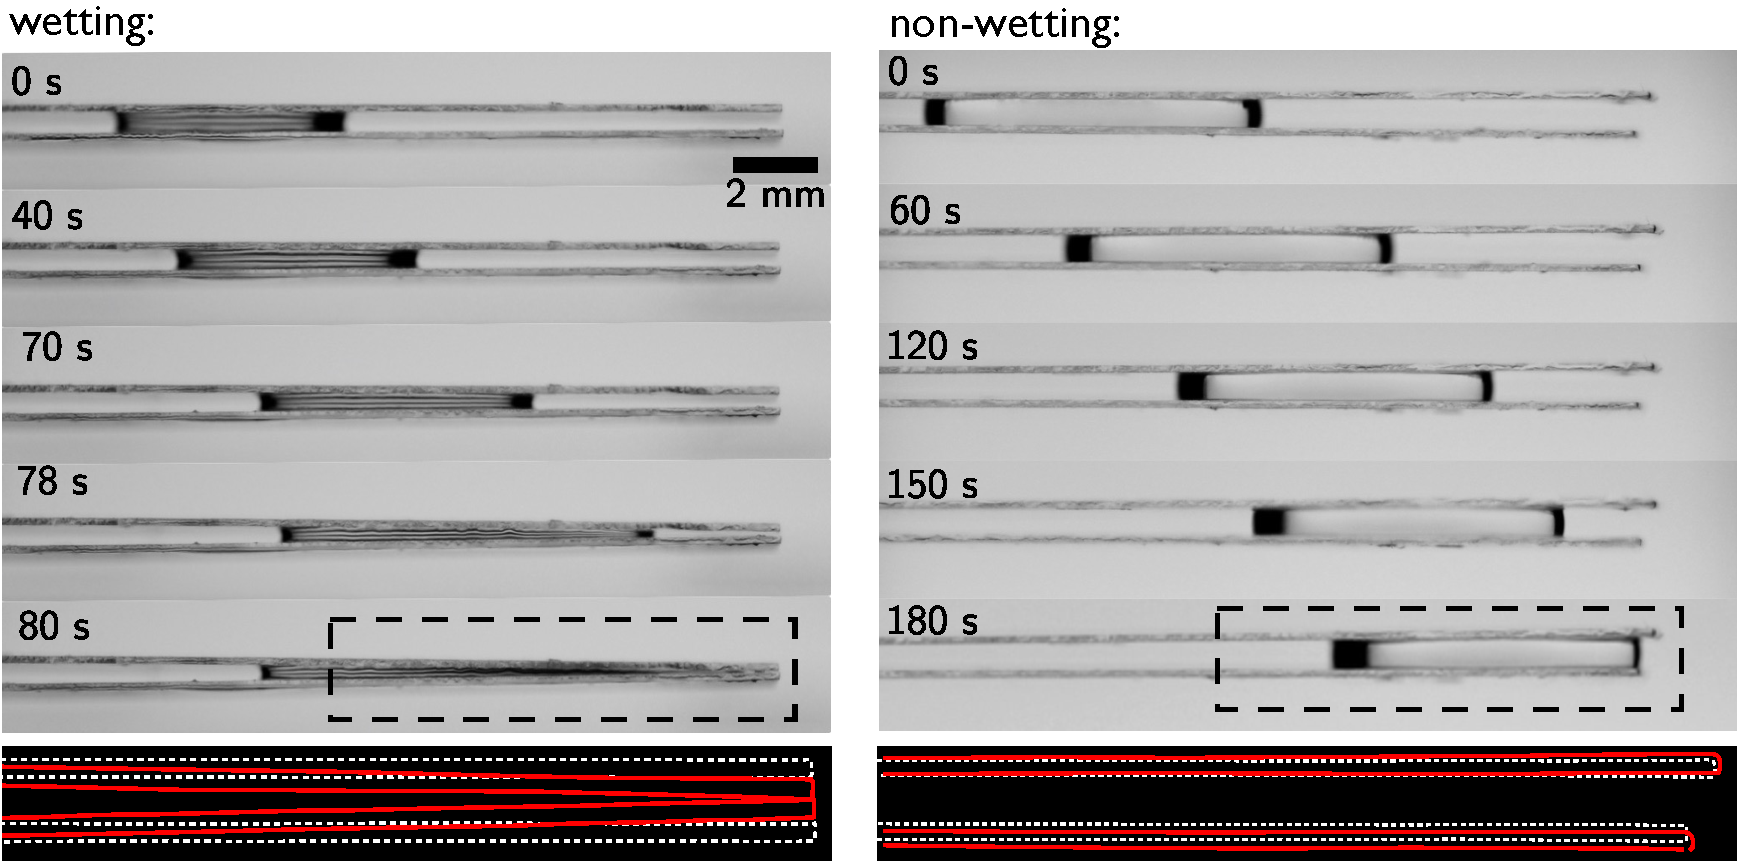
\includegraphics[width = \textwidth]{PoC_expts}
\caption{(top) Experimental demonstration of bendotaxis for a wetting silicone oil droplet (left) and a non-wetting water droplet (right), each between initially parallel, yet deformable, glass cover slips. While the deformation of the channel occurs in the opposite sense in each case (left: inwards, versus right: outwards), the direction of droplet motion is the same. (bottom) Comparison of final channel shape (red lines) with the initial channel shape (dotted white lines) for the section highlighted by the dashed box in the final experiment image.}\label{fig:Ch1:PoC}
\end{figure}


The bendotaxis mechanism described in  \S1.4.2 is reproducible in a simple laboratory experiment, with a channel fabricated using a rigid separator and glass cover slips. Figure~\ref{fig:Ch1:PoC} shows the time series of a wetting silicone oil droplet and of a non-wetting water droplet in such a channel. In both cases, the droplets move towards the free end of the channel. (More experimental details are given in Chapter 3.)

To observe the deflection of the cover slips, we compare their shapes in the final configuration with those prior to the introduction of the droplet (last panel in Figure~\ref{fig:Ch1:PoC}). In the wetting case, both cover slips are deflected inwards, while in the non-wetting case both are deflected outwards -- the deflections are in accord with the above physical description. The observed deflections also provide evidence that motion is not simply caused by the weight of the droplet, which would cause the lower cover slip to deflect downwards in both cases.

%describe what we do in the first half
In the first half of this thesis, we consider the quasi-two-dimensional configuration shown in Figure~\ref{fig:Ch1:PoC} and describe the dynamics of bendotaxis. With a view to the applicability of bendotaxis to anti-fogging surfaces, we focus on the time taken for droplets to be transported. We also consider situations in which the droplet transport is inhibited. Below we provide a more detailed synopsis of the three chapters that make up this first half.

In Chapter 2, we develop a two-dimensional mathematical model for bendotaxis. The physical processes represented by this model are motivated by those relevant in the proof of concept experiments in Figure~\ref{fig:Ch1:PoC}; in particular, we exploit the small aspect ratio of the channel and slenderness of its walls to combine lubrication theory and linear beam theory. By solving the model equations numerically, we verify that our model predicts wettability-independent droplet transport and gain insight into its dynamics; these numerical solutions are contrasted to analytic solutions available in the case of small channel deformations. Finally, we discuss the implications of our model for superhydrophobic surfaces that exploit bendotaxis.

In Chapter 3, we describe an experimental study of bendotaxis. The configuration is the similar to that for the experiments shown in Figure~\ref{fig:Ch1:PoC}, but we systematically vary the channel length, channel thickness, wall bending stiffness, wettability conditions, and liquid viscosity; these experiments provide a robust test of the mathematical model developed in Chapter 2 and offer further insight into the dynamics of bendotaxis.

In Chapter 4, we extend our mathematical model to include two phenomena encountered in Chapters 2 and 3 that can impede droplet transport: firstly, the scenario in which the channel walls touch before the droplet has reached the free end, trapping it indefinitely (so called `geometric trapping'), and, secondly, contact angle hysteresis, which, when sufficiently large, can completely arrest motion. For each of these, we describe the influence on the dynamics, and quantify when the droplet is prevented from reaching the free end. (Each of these effects would be detrimental to the performance of an anti-fogging textured surface exploiting bendotaxis).

\subsection{Bendotaxis in microchannels}

\begin{figure}
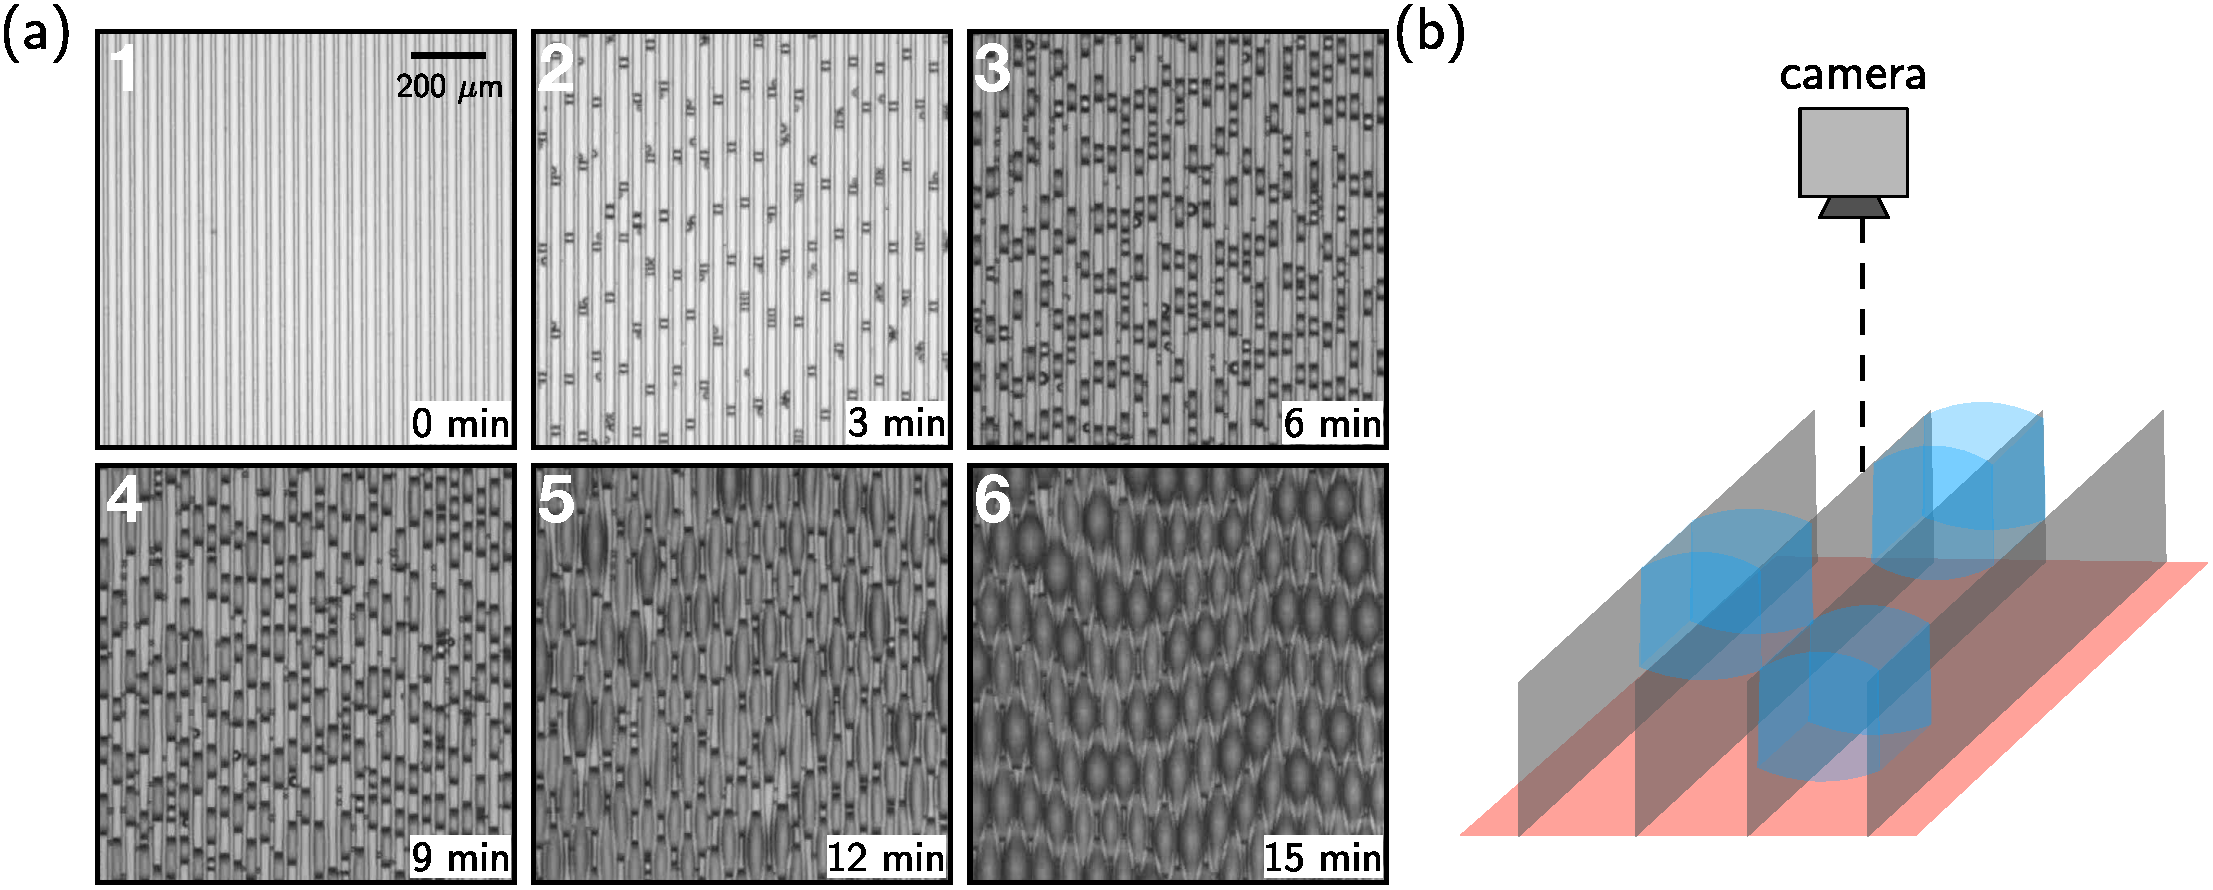
\includegraphics[width =0.95\textwidth]{BrinkmannExperiments}
\caption{Snapshots of experiments performed by~\cite{Seemann2011JPhysCondMat}. Droplets are condensed into an array of initially empty (1), deformable microchannels (the channel walls run vertically in the images, and the setup is shown schematically in (b)). Droplets continue to grow and move towards the open end (out of the page) of the channels (3, 4). Once droplets reach the end closest to the camera (5), their interface curvature relaxes and the light spot in their centre is no longer visible. The final configuration (6) has a lattice-like pattern charaterized by a pairwise mode in the direction perpendicular to the channel walls, as well as a periodic pattern in the parallel direction. We anticipate that this instability shares many features of bendotaxis.}\label{fig:Ch1:MBexpts}
\end{figure}

In the second half of this thesis, we consider how various channel geometries affect the bendotaxis mechanism. Motivation is provided the experiments of~\cite{Seemann2011JPhysCondMat} in which droplets are condensed into micro-channels. These experiments, shown in Figure~\ref{fig:Ch1:MBexpts}, clearly show an instability, and we shall explore the extent to which this instability may illustrate bendotaxis. In addition, these experiments may offer insight into how a superhydrophobic surface whose topographical features exploit bendotaxis to stay fog free might behave. (Superhydrophobic surfaces with flexible topographies have been realised~\citep[see][for example]{Blow2010Langmuir}, but typically do not have the correct geometry to exploit bendotaxis, with features too well separated from one another.)

As seen in the snapshots of these experiments (Figure~\ref{fig:Ch1:MBexpts}(a)), droplets nucleate at the base of a three dimensional array of channels and their upper surface moves towards the free end of the channels (the end closest to the camera, see Figure~\ref{fig:Ch1:MBexpts}(b)). This motion is reminiscent of bendotaxis; in particular, in both the wetting and non-wetting cases, this advancing interface is accompanied by a reduction in liquid pressure there (the channel deformation increases), encouraging flow towards it. While the interface is advancing, the volume of liquid in the channels is increasing as condensation continues. The motion of the (non-wetting) droplets can be inferred from the light patterns within them: when they are between the base and the free end, their interface curvature focusses incoming light and we see a bright spot in their centres (Figure~\ref{fig:Ch1:MBexpts}(a)2--5); once they touch the free end, the interfacial curvature of the droplets relaxes, resulting in a uniform light pattern on their surface (Figure~\ref{fig:Ch1:MBexpts}(a)6).

These experiments pose two questions: firstly, what controls the `weaving' instability seen in Figure~\ref{fig:Ch1:MBexpts}(a)? In Chapter 5, we study a previously-unreported instability mechanism, closely related to the Rayleigh--Plateau instability~\citep{Plateau1873, Rayleigh1879PRSL, Rayleigh1892PhilosMag}  whose mode selection may explain the length scale of this weaving instability.  We develop a mathematical model of a system that exhibits similar behaviour to gain insight into the dynamics of this instability, and describe the influence of the speed at which liquid is condensed into the channels on the mode selection problem.

The second question posed by the experiments of Figure~\ref{fig:Ch1:MBexpts} is: how would multiple droplets in neighbouring channels affect each other's bendotaxis? The deformation resulting from the Laplace pressure of condensed droplets changes not only the width of the channel that contains it, but also the width of the neighbouring channels. For a non-wetting liquid, the neighbouring channels are narrowed, tending to move droplets in those channels towards the base. In turn, this affects the thickness of the next-nearest neighbour to the original channel. By iterating this argument, we might expect a long range ordering in the direction perpendicular to the channel walls. Why then does this happen in a pairwise manner in the experiments of Figure~\ref{fig:Ch1:MBexpts}(a)? In Chapter 6 we describe the interaction between neighbouring channels, each of which would undergo bendotaxis in isolation and use this information to understand the clustering behaviour.

In Chapter 7, we summarize the main results of the thesis and discuss the possibilities for future work.
}

\newcommand{\green}[1]{{\color{green} #1}}
\newcommand{\red}[1]{{\color{red} #1}}
\newcommand{\blue}[1]{{\color{blue} #1}}
\newcommand{\bendability}{\nu}

\newcommand{\upd}{\mathrm{d}}
\newcommand{\ddp}[2]{\frac{\partial #1}{\partial #2}}
\newcommand{\dd}[2]{\frac{\upd #1}{\upd #2}}
\newcommand{\xleft}{x_{-}}
\newcommand{\xright}{x_{+}}

%nb: you need \text{(\theequation)} rather than just (\theequation) if you want the equation number to be in same font as the text (e.g. sans serif)
\newcommand\abcdeqn[2]{\refstepcounter{equation}
     \[
     \label{#1}
     #2
     \eqno{\text{(\theequation)}\text{a,b,c,d}}
     \]
}
\newcommand\abeqn[2]{\refstepcounter{equation}
     \[
     \label{#1}
     #2
     \eqno{\text{(\theequation)}\text{a,b}}
     \]
}


\graphicspath{{./Sections/Chapter2_modelling/figures/}}


%%%%%%%%%%%%%%%%%%%%%%%%
\chapter{Modelling bendotaxis}
In this chapter, we develop and analyse a mathematical model of bendotaxis, motivated by the proof of concept experiments shown in \S1.4.3. We begin by deriving a two-dimensional theoretical model that combines linear elasticity to describe the channel deformations with lubrication theory to describe fluid flow in response to capillary-induced pressure gradient. We then describe a numerical scheme used to solve the model equations and discuss the behaviour of these solutions. Following this, we consider the case of small deflections -- in which analytical progress can be made -- and discuss the implications of our model for droplet removal from deformable channels by bendotaxis.

\section{Theoretical model of bendotaxis}
\begin{figure}[t]
\centering
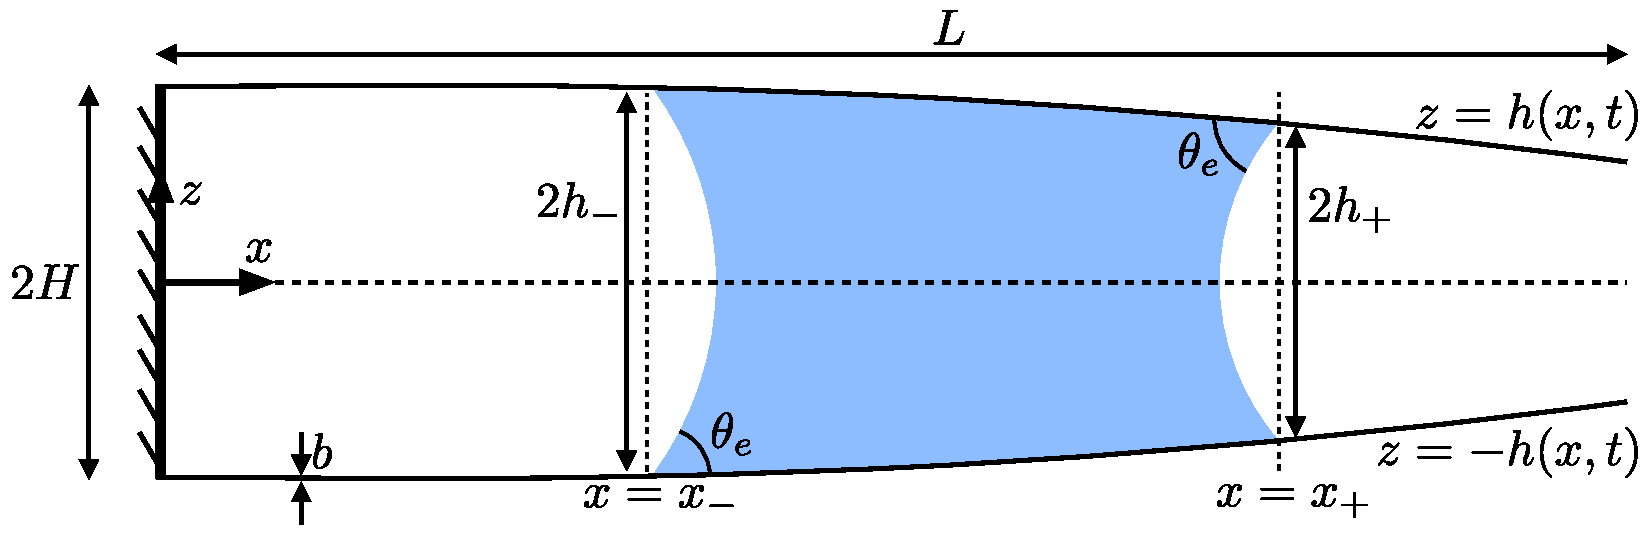
\includegraphics[width = 0.75\textwidth]{Schematic}
\label{fig:Model:Schematic}
\caption{Schematic of a droplet in a flexible channel which has underformed wall separation $2H$ and length $L$, and whose walls have thickness $b$. The menisci contact the walls at perpendicular distances $x = x_{-}(t)$ and $x = x_{+}(t)$ from the clamped end of the channel.}
\end{figure}

In this section, we develop a theoretical model of bendotaxis. We consider the setup shown in Figure~\ref{fig:Model:Schematic}; a channel bounded by two narrow, flexible beams of thickness $b$, length $L$, density $\rho_s$ and Young's modulus $E$, are clamped parallel to one another at a distance $2H$ apart, at one end of the beams. This clamped end defines the $z$-axis, and the axis of the channel (parallel to the undeformed beams) defines the $x$ axis. Although we shall show its effect to be negligible, gravity is initially assumed to act parallel to the $z$-axis.

The channel contains a droplet of liquid of viscosity $\mu$, surface tension $\gamma$ and density $\rho$. The droplet has (two dimensional) volume $\Omega$, and makes a liquid bridge between the channel walls, wetting them over of a region $\xleft(t) < x <\xright(t)$. We assume that the droplet makes a constant contact angle $\theta_e$ with the channel walls (i.e.~we neglect dynamic contact angle effects, and assume there is no contact angle hysteresis).

Table~\ref{T:Chapter2:ExptValues} contains typical experimental values from the experiments shown in Chapter 1 (and discussed further in Chapter 3) of those quantities introduced here.

\def\arraystretch{1.1}%stretch the table
\begin{table}[t]
\begin{center}
\begin{tabular}{| c | c | c | c  |}
\hline
Description & Symbol & Value & SI Units \\ \hline \hline
Droplet surface tension & $\gamma$ & $22\times 10^{-3}$ & N~m\textsuperscript{-1}\\
Young's modulus & $E$ & $63\times 10^9$ & Pa\\
Channel wall thickness & $b$ & $180\times 10^{-6}$ & m\\
Channel half width & $H$ &$ 250\times 10^{-6}$ & m\\
Channel length & $L$  & $25\times 10^{-3}$ &m\\
Liquid density & $\rho_l$ & $960$ & kg~m\textsuperscript{-3}\\
Channel wall density & $\rho_s$ & $2500$ & kg~m\textsuperscript{-3}\\
Droplet viscosity (dynamic) & $\mu$ & $0.096$ & Pa~s  \\
Droplet volume & $\Omega$ & $15\times 10^{-9}$ & m\textsuperscript{3} \\
Contact angle & $\theta_e$ & $0$ & n/a\\
Capillary time scale & $\tau_c$ & $10$ & s \\
Bendotaxis time scale & $\tau$ & $10$ & s\\ \hline
\end{tabular}
\end{center}
\caption{Summary of notation used in this chapter and typical values of the corresponding variables in the proof of concept experiment (\S1.4.3) and experimental study (Chapter 3). }\label{T:Chapter2:ExptValues}
\end{table}
\subsection{A scaling argument}\label{S:Model:Scaling}
Before we derive a detailed mathematical model, we consider a scaling argument, valid for small droplets, to gain theoretical insight.

As discussed in Chapter 1, we expect that droplet motion will be driven by the pressure gradient across it. This pressure gradient arises from a difference in Laplace pressure at the leading and rear menisci. When surface tension forces dominate over gravitational forces (i.e.~when the droplet Bond number is small), the menisci do not deform significantly under the weight of the liquid and they take the shape of semi-circular arcs with interfacial curvatures $\kappa_{\pm} = -\cos \theta_e/h_{\pm}$~\citep{deGennes2004}, where $h_{\pm}$ are the channel half widths at the menisci (Figure~\ref{fig:Model:Schematic}).

The corresponding liquid pressure at each meniscus is $p_{\pm} = -\gamma  \cos \theta_e/h_{\pm}$, and the pressure change across the droplet is
\begin{equation}\label{E:Chapter2:Model:Scaling:PressureChange}
\Delta P = p_{+} - p_{-} = -\gamma \cos \theta_e(1/h_{+} - 1/h_{-}).
\end{equation}

In the case that the droplet volume is small relative to the channel volume, $V = \Omega / (2HL) \ll 1$, the liquid pressure is applied to the beams over a relatively short length, and the resulting channel deformation will be small. The length $\Delta X = \xright - \xleft$ over which the pressure is applied is approximately $\Delta X \approx \Omega/(2H)$ -- equal to the length of the droplet in the undeformed channel -- and we can expand the channel width as
\begin{equation}\label{E:Chapter2:Model:Scaling:ChannelWidthDiff}
h_+ \sim h_- + \alpha \Delta X.
\end{equation}
Here $\alpha$ is the average channel slope across the droplet (whose scaling is to be determined).

Combining~\eqref{E:Chapter2:Model:Scaling:PressureChange} and~\eqref{E:Chapter2:Model:Scaling:ChannelWidthDiff}, the pressure gradient across the droplet can be approximated by
\begin{equation}\label{E:Chapter2:Model:Scaling:PressureChangeExpanded}
\frac{\Delta P}{\xright -  \xleft} \sim  \frac{\Delta P}{\Delta X} \sim \frac{ \alpha \gamma \cos \theta_e \Delta X }{H^2}.
\end{equation}

The channel walls are slender, so their resistance to bending is characterized by their bending stiffness $B = Eb^3/12$~\citep{Howell2009}, and their behaviour can be modelled using linear beam theory. Since the droplet is small, its effect on the channel can be approximated by a point force of magnitude $\gamma \cos \theta_e\Delta X /H$; linear beam theory~\citep{Howell2009} gives the scaling for the angle of a cantilever beam forced by a point force of this magnitude, and bending over a length scale $L$, as
\begin{equation}\label{E:Chapter2:Model:Scaling:AngleScaling}
\alpha \sim\frac{\gamma \cos \theta_e \Delta X}{H} \frac{L^2}{B}.
\end{equation}

Provided that the droplet aspect ratio $\Delta X /H$ is small, lubrication theory~\citep{Leal2007} is applicable for the fluid flow and gives the velocity scale $U$ for the fluid flow as
\begin{equation}\label{E:Chapter2:Model:Scaling:VelocityScale}
U \sim \frac{H^2}{\mu}\frac{\Delta P}{\Delta X}.
\end{equation}

Combining~\eqref{E:Chapter2:Model:Scaling:PressureChangeExpanded},~\eqref{E:Chapter2:Model:Scaling:AngleScaling} and~\eqref{E:Chapter2:Model:Scaling:VelocityScale} gives the time scale $\tau$ for a droplet to move along the length of the channel as
\begin{equation}\label{E:Chapter2:Model:Scaling:TimeScaling}
\tau \sim \frac{L}{U} \sim   \frac{\mu H B}{L \gamma^2 \cos^2 \theta_e \Delta X}.
\end{equation}

The other relevant time scale is the capillary time scale,
\begin{equation}\label{E:Chapter2:Model:Scaling:CapillaryTimeScale}
\tau_c = \frac{\mu L^2}{|\gamma\cos \theta_e| H},
\end{equation}
which can be thought of as the typical time taken for liquid of viscosity $\mu$ and surface tension $\gamma$ to imbibe a distance $L$ in a capillary tube of radius $H$~\citep{Washburn1921PhysRev}.

The ratio between these two time scales (\eqref{E:Chapter2:Model:Scaling:TimeScaling} and~\eqref{E:Chapter2:Model:Scaling:CapillaryTimeScale}) is
\begin{equation}\label{E:Chapter2:Model:Scaling:ScalingResult}
\frac{\tau}{\tau_c}\sim \frac{B}{|\gamma \cos \theta_e|\Delta X}\frac{H^2}{L^3}.
\end{equation}
Note that for relatively undeformable channels (large $B$ or small $\gamma$), this time scale becomes large, and decreases with increasing droplet size $\Delta X$. Perhaps surprisingly, however, $\tau$ decreases with increasing $H$ -- narrower channels exhibit faster bendotaxis. This is the reverse of imbibition, where the decrease in channel permeability with channel width $H$ is more than offset by the increase in capillary driving pressure -- the imbibition time~\eqref{E:Chapter2:Model:Scaling:CapillaryTimeScale} increases with decreasing $H$.

We now turn to our more detailed mathematical model, but we shall return to this scaling argument to understand the results of this model.
\subsection{Mathematical model}\label{S:Theoretical:Model}
We now derive a detailed mathematical model, beginning here with modelling of the flow within the channel. Note that, under the assumption that the channel is symmetric, we only need to consider its half-width, $h(x,t)$, as in Figure~\ref{fig:Model:Schematic}.

\subsubsection{Fluid motion}
We assume that the drop is long and thin, $\Delta X/H \ll 1$, so that lubrication theory~\citep{Leal2007} applies. Within this framework, the local conservation of mass combined with the kinematic boundary condition at the channel walls ensures that the droplet pressure $p(x,t)$ satisfies
\begin{equation}\label{E:Chapter2:Model:MathModel:Fluid:Reynolds}
\ddp{h}{t} = \frac{1}{3\mu}\ddp{}{x}\left(h^3\ddp{p}{x}\right) \qquad \xleft(t) < x < \xright(t).
\end{equation}

We assume that evaporation is negligible. The time scale of evaporation for a sessile droplet on a substrate is $\tau_{e} \sim \rho \Omega/(H D c_v)$ -- where $D$ is the gas phase diffusivity and $c_v$ the vapour concentration at saturation~\citep{Hu2002JPhysChemB}. For an oil-air or oil-water interface, $\tau_{e} \sim \mathcal{O}(1$~hour), which is much longer that the capillary time scale $\tau_c \sim \mathcal{O}(10$~s).  (A confined droplet, whose surface area exposed to the air is reduced because of the channel walls, will evaporate much slower than a sessile droplet; hence $\tau_{e}$ is a lower bound on the evaporative time scale.)

The flux of fluid through the menisci must therefore balance that caused by the motion, giving the kinematic conditions
\begin{equation}\label{E:Chapter2:Model:MathModel:Fluid:Kinematic}
\dd{x_{\pm}}{t} = -\left.\frac{h^2}{3\mu}\ddp{p}{x}\right|_{x = x_{\pm}}.
\end{equation}
Note that these kinematic conditions are only valid when the droplet is not touching either end of the channel (i.e.~when $0 < \xleft < \xright < 1$).

The motion is driven by a difference between the droplet pressure at the menisci. To make progress, we must specify the pressure at these points. As discussed, when the droplet Bond number $\rho g H_0^2/ \gamma \ll 1$, the menisci are approximately arcs of circles with curvatures
\begin{equation}\label{E:Chapter2:Model:MathModel:Fluid:Curvatures}
\kappa_{\pm} = -\frac{\cos \theta_e}{h(x = x_\pm,t)}.
\end{equation}
The pressure boundary conditions imposed on~\eqref{E:Chapter2:Model:MathModel:Fluid:Reynolds} are therefore
\begin{equation}\label{E:Chapter2:Model:MathModel:Fluid:PressureBC}
p =- \frac{\gamma \cos \theta_e}{h} \qquad \text{at}~x = x_{\pm}.
\end{equation}


\subsubsection{Beam modelling}\label{S:Model:MathModel:BeamModelling}
To close our model, we need to describe how the channel deforms in response to an applied droplet pressure. We use linear beam theory~\citep{Howell2009} to do so; this theory is valid provided that the beams are long and slender in comparison to the channel width ($L \gg 2H$ and $b \ll 2H$, respectively) and undergo small deformations in comparison with their length ($H \ll L$). We shall also assume that the channel is much shorter than the bendo-capillary length $\ell_{bc} = \sqrt{B/\gamma}$, so that capillary induced beam deformations remain relatively small (as discussed in \S1.3, systems larger than the bendo-capillary length experience relatively large deformations under capillary forces). In the proof of concept experiments shown in Chapter 1, $L/\ell_{bc} \approx 0.02$ (see Table~\ref{T:Chapter2:ExptValues}).

We shall assume that beam inertia, gravitational forces, and the tension within the beam can be neglected. Here we set out the conditions under which each of these assumptions is valid.

A tension within the beam is induced by the component of the line force from surface tension at the menisci. This tension is constant along the beam~\citep{Howell2009}, except across the menisci $x_{\pm}$, where it experiences a jump of magnitude $|\gamma \cos \theta_e|$. Provided the beams do not interact, there is no tension in the region $\xright < x < L$ (we shall discuss the case of interacting beams in Chapter 4). As a result, the beam tension $T$ scales with $|\gamma \cos \theta_e|$, and the tensile forces within the beam~\citep{Howell2009} scale as
\begin{equation}
T\ddp{^2 h}{x^2} \sim \frac{| \gamma  \cos \theta_e|H}{L^2}.
\end{equation}
Bending forces within the beam scale with $B H/L^4$; the ratio between tensile and bending forces therefore scales with
\begin{equation}
\frac{L^2 \cos \theta_e}{\ell_{bc}^2}.
\end{equation}
Our assumption that $L \ll \ell_{bc}$ means that we can neglect beam tension.

Our neglect of gravitational forces requires careful justification.  We consider the pressure gradient induced by both gravitational and bendo-capillary effects as follows, and show that the latter is dominant. As shown in \S\ref{S:Model:Scaling}, a droplet of volume $\Omega$ which occupies a small portion of the channel ($V = \Omega /(2HL) \ll 1$) induces a bendo-capillary pressure gradient $p_x^{bc} \sim \gamma \cos^2 \theta_e L^2 \Delta X /(BH^3)$. A pressure gradient due to gravity arises from a deflection of the whole assembly under its own weight, $F_g^{\text{beam}} \sim \rho_s g b L$, and that of the drop,$F_g^{\text{drop}} \sim \rho g \Omega$. By considering a cantilever beam weighted down by forces $F_g^{\text{beam}}$ and $F_g^{\text{drop}}$, we find a scaling for this angle to be $\alpha_g \sim (\rho_s b + \rho H V)gL^3 /B$ (relative to the horizontal). The associated pressure gradient is $p_x^g \sim\alpha_g \rho g \sim (\rho_s b + \rho H V) \rho g^2 L^3 /B$. The ratio of these two pressure gradients is $p_x^g /p_x^{bc} \sim (\rho_s b + \rho H V)LH^3/(\rho \Delta X \ell_c^4)$, where $\ell_c = \sqrt{\gamma |\cos \theta_e|/(\rho g)} $ is the capillary length of the system. Typical experimental values (table~\ref{T:Chapter2:ExptValues}), give $p_x^g/p_x^{bc} \approx 0.05$; we therefore neglect bending of the plates under their own weight (or that of the droplet) as a driving mechanism for motion. (Note that a related gravity dominated problem has recently been considered by~\cite{Howell2016JFM}.)

Finally, our assumption that beam inertia is negligible is  valid provided the inertial time scale -- that obtained by balancing beam inertia and bending stiffness, $\tau_{I} \sim \sqrt{\rho_s b L^4 /B} = \mathcal{O}(10^{-3}~\text{s})$ -- is much shorter than the capillary time scale $\tau_c = \mu L^2 /( |\gamma \cos \theta_e|H) = \mathcal{O}(10~\text{s})$.\newline

With the assumptions described above, the channel width $h(x,t)$ satisfies the Euler-Bernoulli equation
\begin{equation}\label{E:Chapter2:Model:MathModel:Beam:EulerBernoulli}
B\ddp{^4 h}{x^4} = q(x,t)
\end{equation}
where $q(x,t)$ is the applied droplet pressure,
\begin{equation}\label{E:Chapter2:Model:MathModel:Beam:EulerBernoulliAppliedPressure}
q(x,t) =\left\{ \begin{array}{l l}
0 & \qquad \text{for}~ 0 < x < \xleft(t),\\
p(x,t) & \qquad\text{for}~ \xleft(t)< x < \xright(t),\\
0 & \qquad \text{for}~ \xright(t) < x < L.
\end{array}\right.
\end{equation}
Note that we have now specified the droplet pressure in terms of the channel shape,
\begin{equation}\label{E:Chapter2:Model:MathModel:Beam:Pressure2Channel}
p(x,t) = B\ddp{^4 h}{x^4} \qquad \text{for}~\xleft(t) < x < \xright(t).
\end{equation}
To proceed, boundary conditions on the beam must be specified. We ensure that the beams are clamped at $x = 0$ by imposing
\begin{equation}\label{E:Chapter2:Model:MathModel:Beam:ClampedEndBC}
h = H\quad \text{and} \quad  \ddp{h}{x} = 0 \quad \text{at}~x = 0.
\end{equation}
At the other end, the beams are free -- they are not subject to any moment or shear -- and we therefore impose
\begin{equation}\label{E:Chapter2:Model:MathModel:Beam:FreeEndBC}
\ddp{^2 h}{x^2} = 0 \quad \text{and} \quad  \ddp{^3 h}{x^3}= 0   \quad \text{at}~x = L.
\end{equation}

It is worth stressing that the asymmetry in the boundary conditions -- clamped conditions at one end, and free conditions at the other -- is an important part of the mechanism responsible for bendotaxis. The asymmetry means that the same force applied further from the clamped end results in a larger deflection -- the channel is effectively `softer' there (although the bending stiffness $B$ is constant along the beam).

Note that when surface tension is sufficiently strong (and the droplet wets the channel, so that the channel walls are brought towards one another by deflections), we expect that the beams may touch during droplet motion. In this case, the boundary conditions~\eqref{E:Chapter2:Model:MathModel:Beam:FreeEndBC} will no longer hold. We postpone any discussion of this scenario until Chapter 4.

We assume that the channel wall separation, slope, and moment are continuous across the menisci,
\begin{equation}\label{E:Chapter2:Model:MathModel:Beam:ContinuityBC}
\left[h\right]_{x_{\pm}^-}^{x_{\pm}^+} = \left[\ddp{h}{x}\right]_{x_{\pm}^-}^{x_{\pm}^+} = \left[\ddp{^2 h}{x^2}\right]_{x_{\pm}^-}^{x_{\pm}^+} = 0.
\end{equation}
where $\left[f\right]_{x_{\pm}^-}^{x_{\pm}^+} = f(x_{\pm}^+,t) -  f(x_{\pm}^-,t)$ denotes the jump in the quantity $f$ across the menisci.

Finally, the line force from surface tension induces a jump in the shear force across the menisci,
\begin{equation}\label{E:Chapter2:Model:MathModel:Beam:shearBC}
B \left[\ddp{^3 h}{x^3 }\right]_{x_{\pm}^-}^{x_{\pm}^+}  = \gamma \sin \theta_e
\end{equation}
However, as the ratio of the right hand side of~\eqref{E:Chapter2:Model:MathModel:Beam:shearBC} to the left hand side scales with
\begin{equation}\label{E:Chapter2:Model:MathModel:Beam:shearBCratio}
\frac{\gamma \cos \theta_e L^3 }{B H} = \frac{L^2}{\ell_{bc}^2}\frac{L}{H} \sin \theta_e,
\end{equation}
we can ignore the line force provided the channel aspect ratio $(H/L) \gg\sin  \theta_e (L/\ell_{bc})^2 $. We assume this holds (in the non-wetting proof of concept experiment, the quantity~\eqref{E:Chapter2:Model:MathModel:Beam:shearBCratio} is approximately 0.05; for the wetting proof of concept experiment we have $\sin \theta_e = 0$), so the final boundary condition on~\eqref{E:Chapter2:Model:MathModel:Beam:EulerBernoulli}--\eqref{E:Chapter2:Model:MathModel:Beam:EulerBernoulliAppliedPressure} is
\begin{equation}\label{E:Chapter2:Model:MathModel:Beam:shearBCfinal}
 \left[\ddp{^3 h}{x^3 }\right]_{x_{\pm}^-}^{x_{\pm}^+}   = 0.
\end{equation}

\subsubsection{Initial conditions}
The problem~\eqref{E:Chapter2:Model:MathModel:Fluid:Reynolds}--\eqref{E:Chapter2:Model:MathModel:Fluid:Kinematic}, \eqref{E:Chapter2:Model:MathModel:Fluid:PressureBC}, and~\eqref{E:Chapter2:Model:MathModel:Beam:EulerBernoulli}--\eqref{E:Chapter2:Model:MathModel:Beam:ContinuityBC},~\eqref{E:Chapter2:Model:MathModel:Beam:shearBCfinal} (for $h(x,t)$, $p(x,t)$, $\xleft(t)$, $\xright(t)$) is closed by specifying initial conditions. We assume that the channel is initially undeformed,
\begin{equation}\label{E:Chapter2:Model:MathModel:IC:IC_BeamShape}
h(x,0) = H.
\end{equation}
The corresponding spatially constant pressure is set by its values at the menisci
\begin{equation}\label{E:Chapter2:Model:MathModel:IC:IC_pressure}
p(x,0) = \frac{\gamma \cos\theta_e}{H}, \quad \xleft^0< x <\xright^0.
\end{equation}
where $x_{\pm}^0$ are the initial meniscus positions
\begin{equation}\label{E:Chapter2:Model:MathModel:IC:IC_Menisci}
x_{\pm}(0) = x_{\pm}^0.
\end{equation}
These initial conditions must be consistent with the droplet volume: if the droplet volume $\Omega$ is specified, it is necessary that
\begin{equation}\label{E:Chapter2:Model:MathModel:IC:Volume}
\Omega = 2H (\xright^0 - \xleft^0).
\end{equation}
Here we have neglected the missing volume contributions from the arcs of the menisci, whose contribution to the droplet volume enters at $\mathcal{O}(H/L)$. %Note that the kinematic conditions~\eqref{E:Chapter2:Model:MathModel:Fluid:Kinematic} ensure that volume is globally conserved, i.e.
%\begin{equation}\label{E:Chapter2:Model:MathModel:IC:VolumeConservation}
%\dd{}{t}\left[\int_{\xleft}^{\xright} h(x,t) dx\right] = 0.
%\end{equation}

\subsection{Non-dimensionalization}\label{S:Chapter2:Model:NonDim}
We non-dimensionalize the problem by introducing dimensionless variables
\begin{equation}\label{E:Chapter2:Model:NonDim:Scalings}
\hat{x}= \frac{1}{L}x, \quad \hat{x}_{\pm} = \frac{1}{L}x_{\pm}, \quad \hat{h} = \frac{1}{H}h, \quad \hat{t} = \frac{1}{\tau_c}t, \quad \hat{p} = \frac{L^4}{B H}p,
\end{equation}
where we recall $\tau_c = \mu L^2 /(|\gamma \cos \theta_e |H)$.

Note that we have chosen to non-dimensionalize the pressure $p$ with the natural scale that emerges in the beam equation~\eqref{E:Chapter2:Model:MathModel:Beam:Pressure2Channel} rather than the scale which emerges in the Laplace pressure condition~\eqref{E:Chapter2:Model:MathModel:Fluid:PressureBC}.

By combining~\eqref{E:Chapter2:Model:MathModel:Fluid:Reynolds} and~\eqref{E:Chapter2:Model:MathModel:Beam:EulerBernoulli} and inserting dimensionless variables~\eqref{E:Chapter2:Model:NonDim:Scalings}, we find that the dimensionless channel half width $\hat{h}(\hat{x}, \hat{t})$ satisfies
\begin{align}
0 &= \ddp{^4\hat{h}}{\hat{x}^4} & &0 < \hat{x} < \hat{x}_{-}(\hat{t}),\label{E:Chapter2:Model:NonDim:CombinedEq1} \\
\ddp{\hat{h}}{\hat{t}} &=  \frac{1}{3|\nu|}\ddp{}{\hat{x}}\left(\hat{h}^3 \ddp{^5 \hat{h}}{\hat{x}^5}\right) ,  & &\hat{x}_{-}(\hat{t}) < \hat{x} <  \hat{x}_{+}(\hat{t}),\label{E:Chapter2:Model:NonDim:CombinedEq2}\\
\qquad \qquad0 &= \ddp{^4\hat{h}}{\hat{x}^4} &  &  \hat{x}_{+}(\hat{t}) < \hat{x} < 1.\label{E:Chapter2:Model:NonDim:CombinedEq3}
\end{align}
Here the dimensionless parameter
\begin{equation}\label{E:Chapter2:Model:NonDim:nuDefn}
\nu = \frac{\gamma \cos \theta_e L^4}{B H^2}
\end{equation}
characterizes the ability of the droplet surface tension to bend the channel walls. It is through the parameter $\bendability$ that the model equations `see' the wettability conditions: $\bendability$ is positive for wetting conditions ($\cos \theta_e > 0$) and negative for non-wetting conditions ($\cos \theta_e < 0$). We refer to the parameter $\nu$ as the channel `bendability', although it is closely related to the reciprocal of the elastocapillary number identified by~\cite{Mastrangelo1993JMEMS}. Note that the sixth order partial differential equation (PDE) in~\eqref{E:Chapter2:Model:NonDim:CombinedEq2} is similar to that considered in other studies of elastocapillary dynamics \cite[see][for example]{Flitton2004EJApplMech, Duprat2011JFM, Aristoff2011IntJNonlinMech, Taroni2012JFM}.

In terms of the dimensionless variables, the kinematic conditions~\eqref{E:Chapter2:Model:MathModel:Fluid:Kinematic}  read
\begin{equation}\label{E:Chapter2:Model:NonDim:Kinematic}
\dd{\hat{x}_{\pm}}{\hat{t}}  = \left.\frac{1}{3|\nu|}\ddp{^5\hat{h}}{\hat{x}^5} \right|_{\hat{x} = \hat{x}_{\pm}},
\end{equation}
and the channel shape boundary conditions~\eqref{E:Chapter2:Model:MathModel:Beam:ClampedEndBC}--\eqref{E:Chapter2:Model:MathModel:Beam:ContinuityBC} and~\eqref{E:Chapter2:Model:MathModel:Beam:shearBCfinal} read
\begin{align}
\hat{h} &= 1,\quad \ddp{\hat{h}}{\hat{x}} = 0, & & \text{at}~ \hat{x} = 0,\label{E:Chapter2:Model:NonDim:BCClamped}\\
\ddp{^2 \hat{h}}{\hat{x}^2} &= 0, \quad\ddp{^3\hat{h}}{\hat{x}^3} = 0, & &   \text{at}~ \hat{x} = 1\label{E:Chapter2:Model:NonDim:BCFree},
\end{align}
\abcdeqn{E:Chapter2:Model:NonDim:BCContinuity}{
\left[\hat{h}\right]_{\hat{x}_{\pm}^-}^{\hat{x}_{\pm}^+} = \left[\ddp{\hat{h}}{\hat{x}}\right]_{\hat{x}_{\pm}^-}^{\hat{x}_{\pm}^+} = \left[\ddp{^2 \hat{h}}{\hat{x}^2}\right]_{\hat{x}_{\pm}^-}^{\hat{x}_{\pm}^+} = \left[\ddp{^3 \hat{h}}{\hat{x}^3 }\right]_{\hat{x}_{\pm}^-}^{\hat{x}_{\pm}^+} = 0.}
The dimensionless version of the pressure boundary conditions~\eqref{E:Chapter2:Model:MathModel:Fluid:PressureBC}, expressed in terms of the channel width (using~\eqref{E:Chapter2:Model:MathModel:Beam:Pressure2Channel}) are
\begin{equation}\label{E:Chapter2:Model:NonDim:BCPressure}
\left.\ddp{^4 \hat{h}}{\hat{x}^4}\right|_{\hat{x} = \hat{x}_{\pm}} = -\frac{\nu}{\hat{h}(\hat{x} = \hat{x}_{\pm})}.
\end{equation}
Finally, the dimensionless initial conditions are
\begin{equation}\label{E:Chapter2:Model:NonDim:IC}
\hat{h}(\hat{x}, 0) = 1, \qquad \hat{x}_{\pm}(0) =\hat{x}_{\pm}^0 = \frac{x_{\pm}^0}{L}.
\end{equation}

The problem~\eqref{E:Chapter2:Model:NonDim:CombinedEq1}--\eqref{E:Chapter2:Model:NonDim:IC} (for $h(x,t), \xleft(t), \xright(t)$ -- the pressure $p(x,t)$ has been eliminated via the Euler-Bernoulli equation) has three dimensionless parameters: the bendability $\nu$ and the initial conditions on the menisci $\hat{x}_{\pm}^0$. The latter are related to the relative droplet volume $V = \hat{x}_+^0 - \hat{x}_-^0$, which characterises the proportion of the channel occupied by the droplet. Note that the kinematic boundary condition~\eqref{E:Chapter2:Model:NonDim:Kinematic} ensures that
\begin{equation}
V = \int_{\hat{x}_-}^{\hat{x}_+}\hat{h}(\hat{x},\hat{t})~\mathrm{d}\hat{x}
\end{equation}
holds at all times. We shall typically use ($\nu, \hat{x}_+^0, V)$ (rather than $(\nu, \hat{x}_+^0, \hat{x}_-^0)$) as the set of dimensionless parameters.

Henceforth, hats are dropped and variables are assumed to be dimensionless, unless otherwise stated.


\section{Numerical solutions}
To verify that the model described in the last section does indeed lead to spontaneous transport of droplets to the free end of the channel regardless of wettability, and to analyse the dynamic behaviour, we begin by solving the system of the model equations~\eqref{E:Chapter2:Model:NonDim:CombinedEq1}--\eqref{E:Chapter2:Model:NonDim:CombinedEq3}, numerically, subject to boundary conditions~\eqref{E:Chapter2:Model:NonDim:Kinematic}--\eqref{E:Chapter2:Model:NonDim:BCPressure}, and initial conditions~\eqref{E:Chapter2:Model:NonDim:IC}.
%In this section, we describe the techniques employed to solve these equations numerically and present a phenomenology characterising the behaviours of solutions as the parameters $\nu$ and $V$ are varied.
\subsection{Numerical scheme}\label{S:Ch2:Numerics:Scheme}
Our numerical scheme involves three steps. We first `integrate out' the dry regions ($0 < x < \xleft$ and $\xright < x < 1$), which leaves an equivalent problem defined only in the drop region $\xleft < x < \xright$. This problem is then transformed onto a fixed domain and re-written in a flux-conservative form. We discretize the resulting problem in space, giving a system of ordinary differential equations (ODEs), which are solved numerically using the method of lines~\citep{Schiesser1991}. In this section, we describe each of these steps in detail.

\subsubsection{Isolating the drop region}\label{S:Ch2:Numerics:Scheme:ReducedProblem}
We begin by reducing the problem to one defined only on the drop region, $\xleft < x < \xright$. This is possible because the solutions in the dry regions ($0 < x < \xleft$ and $\xright < x < 1$) may be found analytically and used to give explicit expressions for effective boundary conditions at the menisci which encode the behaviour of the adjacent dry region.

In more detail, the position of the channel walls in the dry regions are simply cubic functions of $x$ with coefficients dependent on the beam shape in the drop region and the meniscus positions. By solving~\eqref{E:Chapter2:Model:NonDim:CombinedEq1} alongside~\eqref{E:Chapter2:Model:NonDim:BCClamped} and~\eqref{E:Chapter2:Model:NonDim:BCContinuity}a,b, the shape in the dry region $0 < x < \xleft$ can be expressed in terms of the shape in the drop region as
\begin{equation}\label{E:Chapter2:Numerics:SchemE:Chapter2:Reduced:ShapeLower}
h(x,t) = \left. \left( x \ddp{h}{x} - 2 h + 2\right) \right|_{x = \xleft} \left(\frac{x}{\xleft}\right)^3 - \left. \left( x \ddp{h}{x} - 3 h + 3\right) \right|_{x = \xleft}\left(\frac{x}{\xleft}\right)^2 + 1.
\end{equation}
Imposing~\eqref{E:Chapter2:Model:NonDim:BCContinuity}c,d at $x = \xleft$ is then equivalent to imposing
\begin{equation}\label{E:Chapter2:Numerics:SchemE:Chapter2:Reduced:EffectiveBCLower}
\ddp{^2 h}{x^2} = \frac{2}{\xleft^2}\left(2\xleft \ddp{h}{x} - 3h + 3\right), \quad \ddp{^3 h}{x^2} = \frac{6}{\xleft^3}\left(\xleft \ddp{h}{x} - 2h + 2\right) \quad \text{at}~x = \xleft.
\end{equation}

Similarly, solving~\eqref{E:Chapter2:Model:NonDim:CombinedEq3} alongside~\eqref{E:Chapter2:Model:NonDim:BCFree} and~\eqref{E:Chapter2:Model:NonDim:BCContinuity}a,b gives the shape in the dry region $\xright < x < 1$ as
\begin{equation}\label{E:Chapter2:Numerics:SchemE:Chapter2:Reduced:ShapeUpper}
h(x,t) = \left.\ddp{h}{x}\right|_{x = \xright} (x - \xright)+ \left.h\right|_{x = \xright},
\end{equation}
which, in turn, shows that~\eqref{E:Chapter2:Model:NonDim:BCContinuity}c,d are equivalent to requiring
\begin{equation}\label{E:Chapter2:Numerics:SchemE:Chapter2:Reduced:EffectiveBCUpper}
\ddp{^2 h}{x^2} = 0, \quad \ddp{^3 h}{x^3} = 0 \quad \text{at}~x = \xright.
\end{equation}
(Note that these effective boundary conditions at $x = x_{\pm}$ are identical to the free boundary conditions~\eqref{E:Chapter2:Model:NonDim:BCFree} which apply at $x = 1$: provided the beams do not interact, the droplet has no information about the channel shape in the dry region $\xright < x < 1$.)


With~\eqref{E:Chapter2:Numerics:SchemE:Chapter2:Reduced:EffectiveBCLower} and~\eqref{E:Chapter2:Numerics:SchemE:Chapter2:Reduced:EffectiveBCUpper}, we have a complete system that involves only the drop region. In summary, the `drop-only' problem to solve is
\begin{equation}\label{E:Chapter2:Numerics:SchemE:Chapter2:Reduced:ReducedProblemPDE}
\ddp{h}{t} = \frac{1}{3|\nu|}\ddp{}{x}\left(h^3 \ddp{^5 h}{x^5}\right) \qquad \text{in}~\xleft(t) < x < \xright(t)
\end{equation}
alongside pressure boundary conditions,
\begin{equation}
\ddp{^4 h}{x^4} = \frac{-\nu}{h} \quad \text{at}~x = x_{\pm},
\end{equation}
and the effective boundary conditions~\eqref{E:Chapter2:Numerics:SchemE:Chapter2:Reduced:EffectiveBCLower} and~\eqref{E:Chapter2:Numerics:SchemE:Chapter2:Reduced:EffectiveBCUpper}. The kinematic conditions
\begin{equation}\label{E:Chapter2:Numerics:SchemE:Chapter2:Reduced:ReducedProblemKinematic}
\dd{x_{\pm}}{t} =\left. \frac{-h^2}{3|\nu|}\ddp{^5 h}{x^5}\right|_{x = x_{\pm}}
\end{equation}
still hold, as do the initial conditions
\begin{equation}\label{E:Chapter2:Numerics:SchemE:Chapter2:Reduced:ReducedProblemIC}
 x_{\pm}(0) = x_\pm^0, \quad h(x,0) = 1.
\end{equation}
Once the problem~\eqref{E:Chapter2:Numerics:SchemE:Chapter2:Reduced:EffectiveBCLower},~\eqref{E:Chapter2:Numerics:SchemE:Chapter2:Reduced:EffectiveBCUpper},~\eqref{E:Chapter2:Numerics:SchemE:Chapter2:Reduced:ReducedProblemPDE}--\eqref{E:Chapter2:Numerics:SchemE:Chapter2:Reduced:ReducedProblemIC} has been solved, the shape of the whole channel can be re-constructed from~\eqref{E:Chapter2:Numerics:SchemE:Chapter2:Reduced:ShapeLower} and~\eqref{E:Chapter2:Numerics:SchemE:Chapter2:Reduced:ShapeUpper}.

\subsubsection{Flux conservative form}
The drop-only problem is transformed from the time dependent domain $\xleft(t) < x < \xright(t)$ to a time-independent domain by letting
\begin{equation}\label{E:Chapter2:Numerics:SchemE:Chapter2:FluxConservativE:Chapter2:SpaceScaling}
z = \frac{x - \xleft(t)}{l(t)}, \qquad 0 < z < 1,
\end{equation}
where $l(t) = \xright(t) - \xleft(t)$ is the drop length.

Since $z$ is time-dependent, the transformation~\eqref{E:Chapter2:Numerics:SchemE:Chapter2:FluxConservativE:Chapter2:SpaceScaling} introduces additional advective terms in~\eqref{E:Chapter2:Numerics:SchemE:Chapter2:Reduced:ReducedProblemPDE}; the time derivatives in the two co-ordinate systems are related by
\begin{equation}\label{E:Chapter2:Numerics:SchemE:Chapter2:FluxConservativE:Chapter2:AdvectiveDerivative}
\left(\ddp{}{t}\right)_{x} =\left(\ddp{}{t}\right)_{z} -\frac{1}{l(t)}\left[z\dd{\xright}{t} + (1-z)\dd{\xleft}{t}       \right]\ddp{}{z},
\end{equation}
where $\left(.\right)_{\xi}$ refers to the derivative with  $\xi$ held constant. Spatial derivatives are straightforward, since
\begin{equation}\label{E:Chapter2:Numerics:SchemE:Chapter2:FluxConservativE:Chapter2:SpatialDerivative}
\left(\ddp{}{x} \right)_t= \frac{1}{l(t)}\left(\ddp{}{z}\right)_t.
\end{equation}
By introducing
\begin{equation}\label{E:Chapter2:Numerics:SchemE:Chapter2:FluxConservativE:Chapter2:Transformation}
U(z,t) = l(t)h(x,t),
\end{equation}
the PDE~\eqref{E:Chapter2:Numerics:SchemE:Chapter2:Reduced:ReducedProblemPDE} is transformed to the flux-conservative form:
\begin{equation}\label{E:Chapter2:Numerics:SchemE:Chapter2:FluxConservativE:Chapter2:FluxConservativeForm}
\ddp{U}{t} + \ddp{Q}{z} = 0,
\end{equation}
where
\begin{equation}\label{E:Chapter2:Numerics:SchemE:Chapter2:FluxConservativE:Chapter2:FluxExpression}
Q = -\frac{1}{l}\left[\frac{1}{3|\nu|}\frac{U^3}{l^8}\ddp{^5 U}{z^5}  + Uz\dd{\xright}{t} + U(1-z)\dd{\xleft}{t}\right]
\end{equation}
plays the role of the flux.

The PDE~\eqref{E:Chapter2:Numerics:SchemE:Chapter2:FluxConservativE:Chapter2:FluxConservativeForm} is solved alongside boundary conditions
\begin{align}
\ddp{^2 U}{z^2} &= \frac{2l}{\xleft^2}\left(2\xleft \ddp{U}{z} - 3lU + 3l^2\right),\label{E:Chapter2:Numerics:SchemE:Chapter2:FluxConservativE:Chapter2:LowerBC1} \\
\ddp{^3 U}{z^3} &= \frac{6l^2}{\xleft^3}\left(\xleft \ddp{U}{z} - 2lU + 2l^2\right), \label{E:Chapter2:Numerics:SchemE:Chapter2:FluxConservativE:Chapter2:LowerBC2} \\
 \ddp{^4 U}{z^4} &= \frac{-\nu l^6}{U},\label{E:Chapter2:Numerics:SchemE:Chapter2:FluxConservativE:Chapter2:LowerBC3}
\end{align}
at $z = 0$, and
\begin{equation}\label{E:Chapter2:Numerics:SchemE:Chapter2:FluxConservativE:Chapter2:UpperBC}
\ddp{^2 U}{z^2} = 0,\qquad \ddp{^3 U}{z^3} = 0, \qquad   \ddp{^4 U}{z^4} = \frac{-\nu l^6}{U},
\end{equation}
at $z = 1$. The kinematic conditions are
\begin{equation}\label{E:Chapter2:Numerics:SchemE:Chapter2:FluxConservativE:Chapter2:Kinematic}
\dd{\xleft}{t} = -\left.\frac{1}{3|\nu|}\frac{U^2}{l^8}\ddp{^5 U}{z^5}\right|_{z = 0}, \qquad \dd{\xright}{t} = -\left.\frac{1}{3|\nu|}\frac{U^2}{l^8}\ddp{^5 U}{z^5}\right|_{z = 1}.
\end{equation}
\subsubsection{Method of lines}

We solve the PDE~\eqref{E:Chapter2:Numerics:SchemE:Chapter2:FluxConservativE:Chapter2:FluxConservativeForm} numerically by discretizing in space: the $z$-domain is divided into a grid of $n$ cells of equal length $\Delta z = 1/n$ with cell centres $z_j = (j - 1/2)\Delta z$ for $j = 1,\dots, n$, and cell edges at $z_{j+1/2} = j\Delta z$ for $j = 0, \dots n$. $U(z,t)$ is approximated at the centre of each cell by $U_j = U(z_j, t)$.

Three ghost points are introduced at each end of the domain (corresponding to cell centres indexed by $j = -2, -1, 0$ and $j = n+1, n+2, n+3$, respectively). By approximating $U$ appropriately at these points, we implement the boundary conditions~\eqref{E:Chapter2:Numerics:SchemE:Chapter2:FluxConservativE:Chapter2:LowerBC1}--\eqref{E:Chapter2:Numerics:SchemE:Chapter2:FluxConservativE:Chapter2:UpperBC}.

The flux $Q$ is approximated at the edges of each cell by $Q_{j+1/2} = Q(z_{j+1/2},t)$. To evaluate the fifth derivative in~\eqref{E:Chapter2:Numerics:SchemE:Chapter2:FluxConservativE:Chapter2:FluxExpression}, we use second-order centred finite differences of $U_j$, $j = -2,\dots, n+3$. Following the positivity preserving scheme described by~\cite{Zhornitskaya2006SIAMNA}, we approximate $U^3$ at the cell centres by $2U_j^2 U_{j+1}^2/(U_j + U_{j+1})$, and approximate $U$ at cell centres by $(U_j +U_{j+1})/2$.

The finite difference discretization results in a system of $n$ ODEs,
\begin{equation}\label{E:Ch2:Numerics:Scheme:DiscretizedODEs}
\dd{U_j}{t} = -\frac{Q_{j + 1/2} - Q_{j -1/2}}{\Delta z}, \qquad j = 1,\dots n,
\end{equation}
which are coupled to the kinematic conditions~\eqref{E:Chapter2:Numerics:SchemE:Chapter2:FluxConservativE:Chapter2:Kinematic}, giving a system of $n + 2$ ODEs. The fifth derivatives in the kinematic conditions are approximated using the same second-order centred finite differences as for the flux, and the $U^2$ terms are approximated using one sided finite differences on the internal grid points (we find that a one-sided approximation results in reduced numerical errors in conservation of mass, compared to a centred approximation).

The system of ODEs is solved numerically using the stiff ODE solving routine \texttt{ODE15s} routine implemented in \textsc{matlab}. A stiff ODE solver is necessary because of the different time scales in the problem; as we shall see, there is a short (early) time scale on which the beams respond to an initial torque imbalance, and a longer time scale on which the droplet moves towards the free end of the channel.

To improve the speed of the \texttt{ODE15s} routine, we specify the Jacobian of the system of ODEs. This is computed at each time-step using complex step differentiation~\citep{Shampine2007ACM}.

Typical computation time is on the order of seconds (Figure~\ref{fig:Ch2:Numerics:Scheme:SpeedTests}(b)) but grows rapidly as the dimensionless drop length $l$ approaches zero, owing to sensitive dependence of the flux $Q$ on this quantity.

The integration continues until either the channel ends touch (in which case $h(x = 1,t) = 0$, and the free end conditions~\eqref{E:Chapter2:Model:MathModel:Beam:FreeEndBC} are no longer valid), or the droplet touches one end of the channel (in which case $\xright = 1$ or $\xleft = 0$, and the kinematic conditions~\eqref{E:Chapter2:Model:MathModel:Fluid:Kinematic} are no longer valid). Note that, whilst we expect the droplet will always eventually move towards the free end of the channel, during the early phase the menisci move in opposite directions and it is therefore possible that a droplet starting sufficiently close to the clamped end will make contact with it. We denote by $t_e$ the (model, rather than clock) time at which the integration finishes.

At each time-step, we compute the volume of the droplet as
\begin{equation}
M(t) = \Delta z\sum_{i = 1}^n U_j(t).
\end{equation}
As a proxy for the numerical error, we compute the maximum percentage mass change (loss or gain, from its initial value of $V$) during the temporal integration as
\begin{equation}
\Delta M = 100 \times \max_{0 < t < t_e} \left(\frac{|M(t)- V|}{V}\right)
\end{equation}
By integrating the system of equations~\eqref{E:Ch2:Numerics:Scheme:DiscretizedODEs} until $t = t_e$ repeatedly with a different number of grid points $n$ (but the same parameters $\nu, V, \xright^0$),
can compute the percentage mass change as a function of $n$. According to this metric the convergence is indeed second order in $\Delta z = 1/n$ (see Figure~\ref{fig:Ch2:Numerics:Scheme:SpeedTests}).
\begin{figure}[t]
\centering
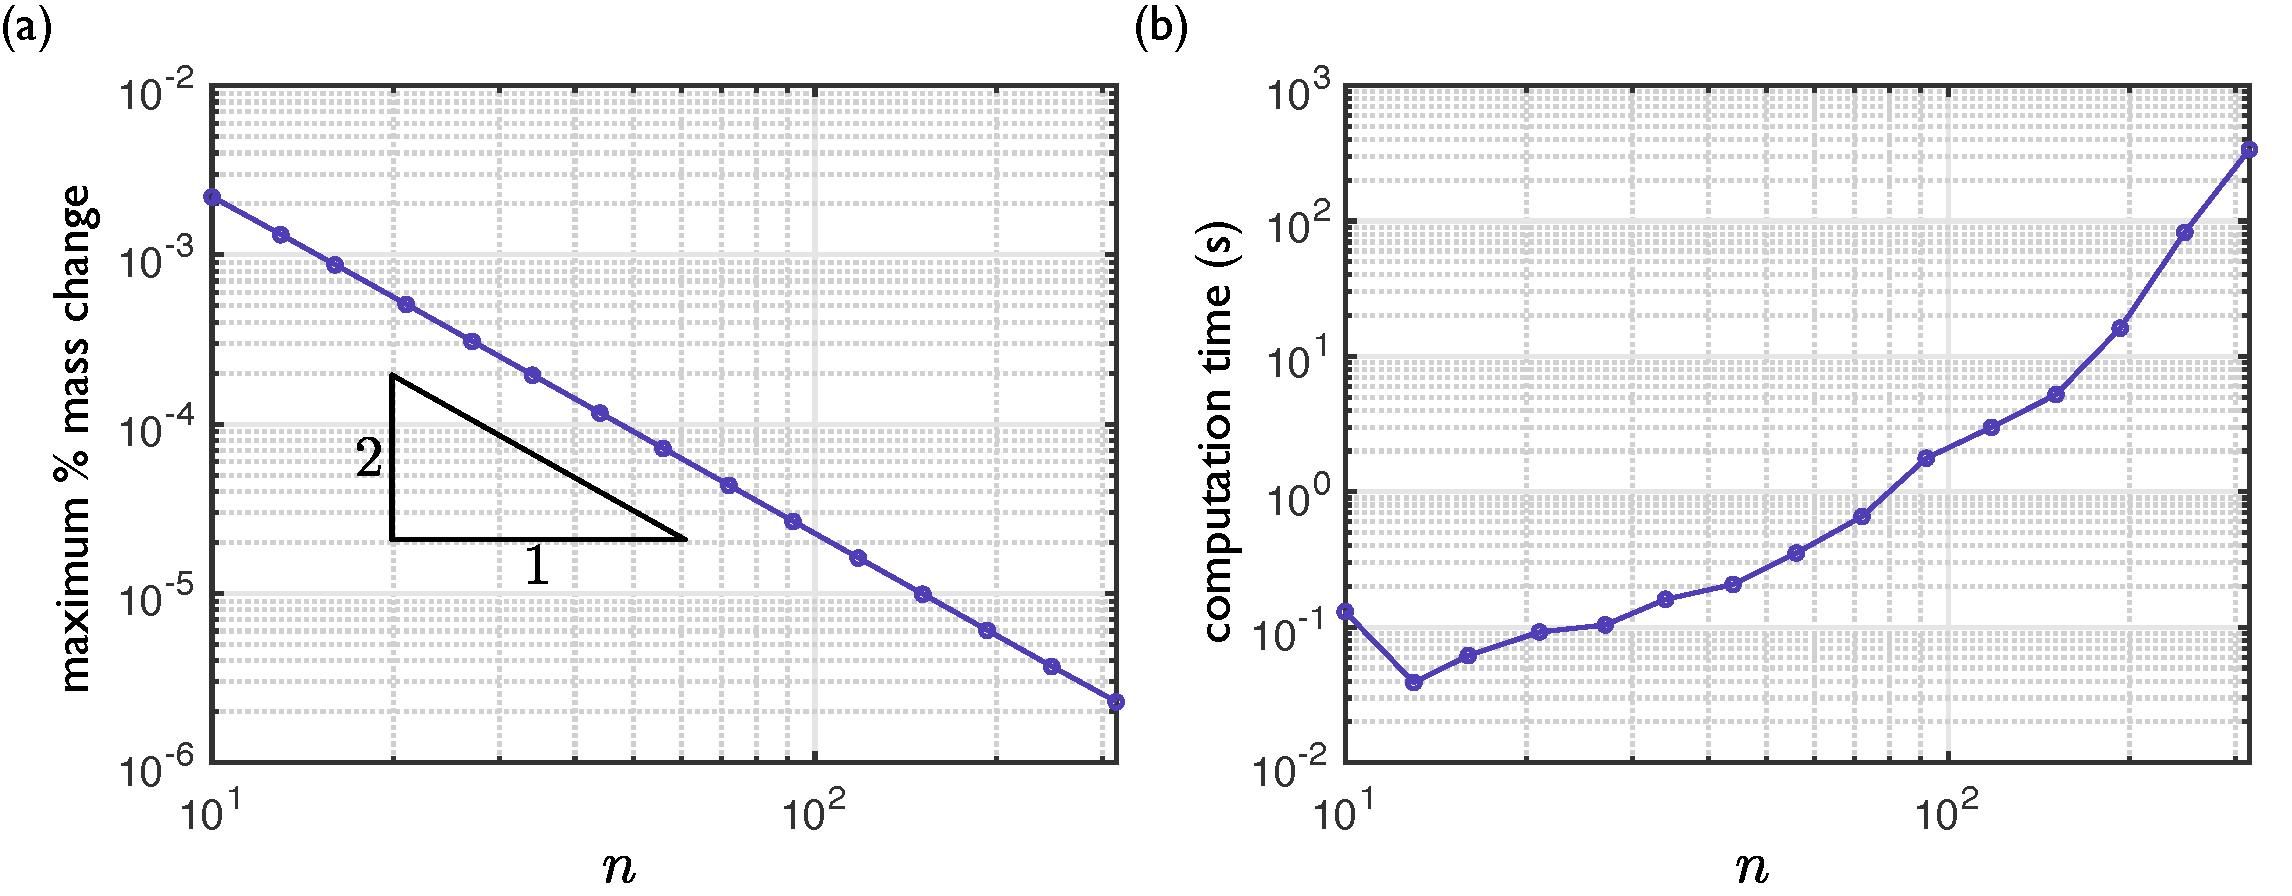
\includegraphics[width = \textwidth]{SpeedTests}
\caption{Plot of (a) $\Delta M$, the maximum percentage mass change, and (b) computation time plotted as a function of the number of grid points $n$ in numerical solutions (obtained using the method of lines) of the equations~\eqref{E:Chapter2:Model:NonDim:CombinedEq1}--\eqref{E:Chapter2:Model:NonDim:CombinedEq3},~\eqref{E:Chapter2:Model:NonDim:Kinematic}, \eqref{E:Chapter2:Model:NonDim:BCClamped}--\eqref{E:Chapter2:Model:NonDim:IC}  with $\nu = 10, V = 0.2 $ and $\xright^0 = 0.8$.}\label{fig:Ch2:Numerics:Scheme:SpeedTests}
\end{figure}


\subsection{Numerical experiments}\label{S:Ch2:Numerics:Experiments}
\begin{figure}[h!]
\centering
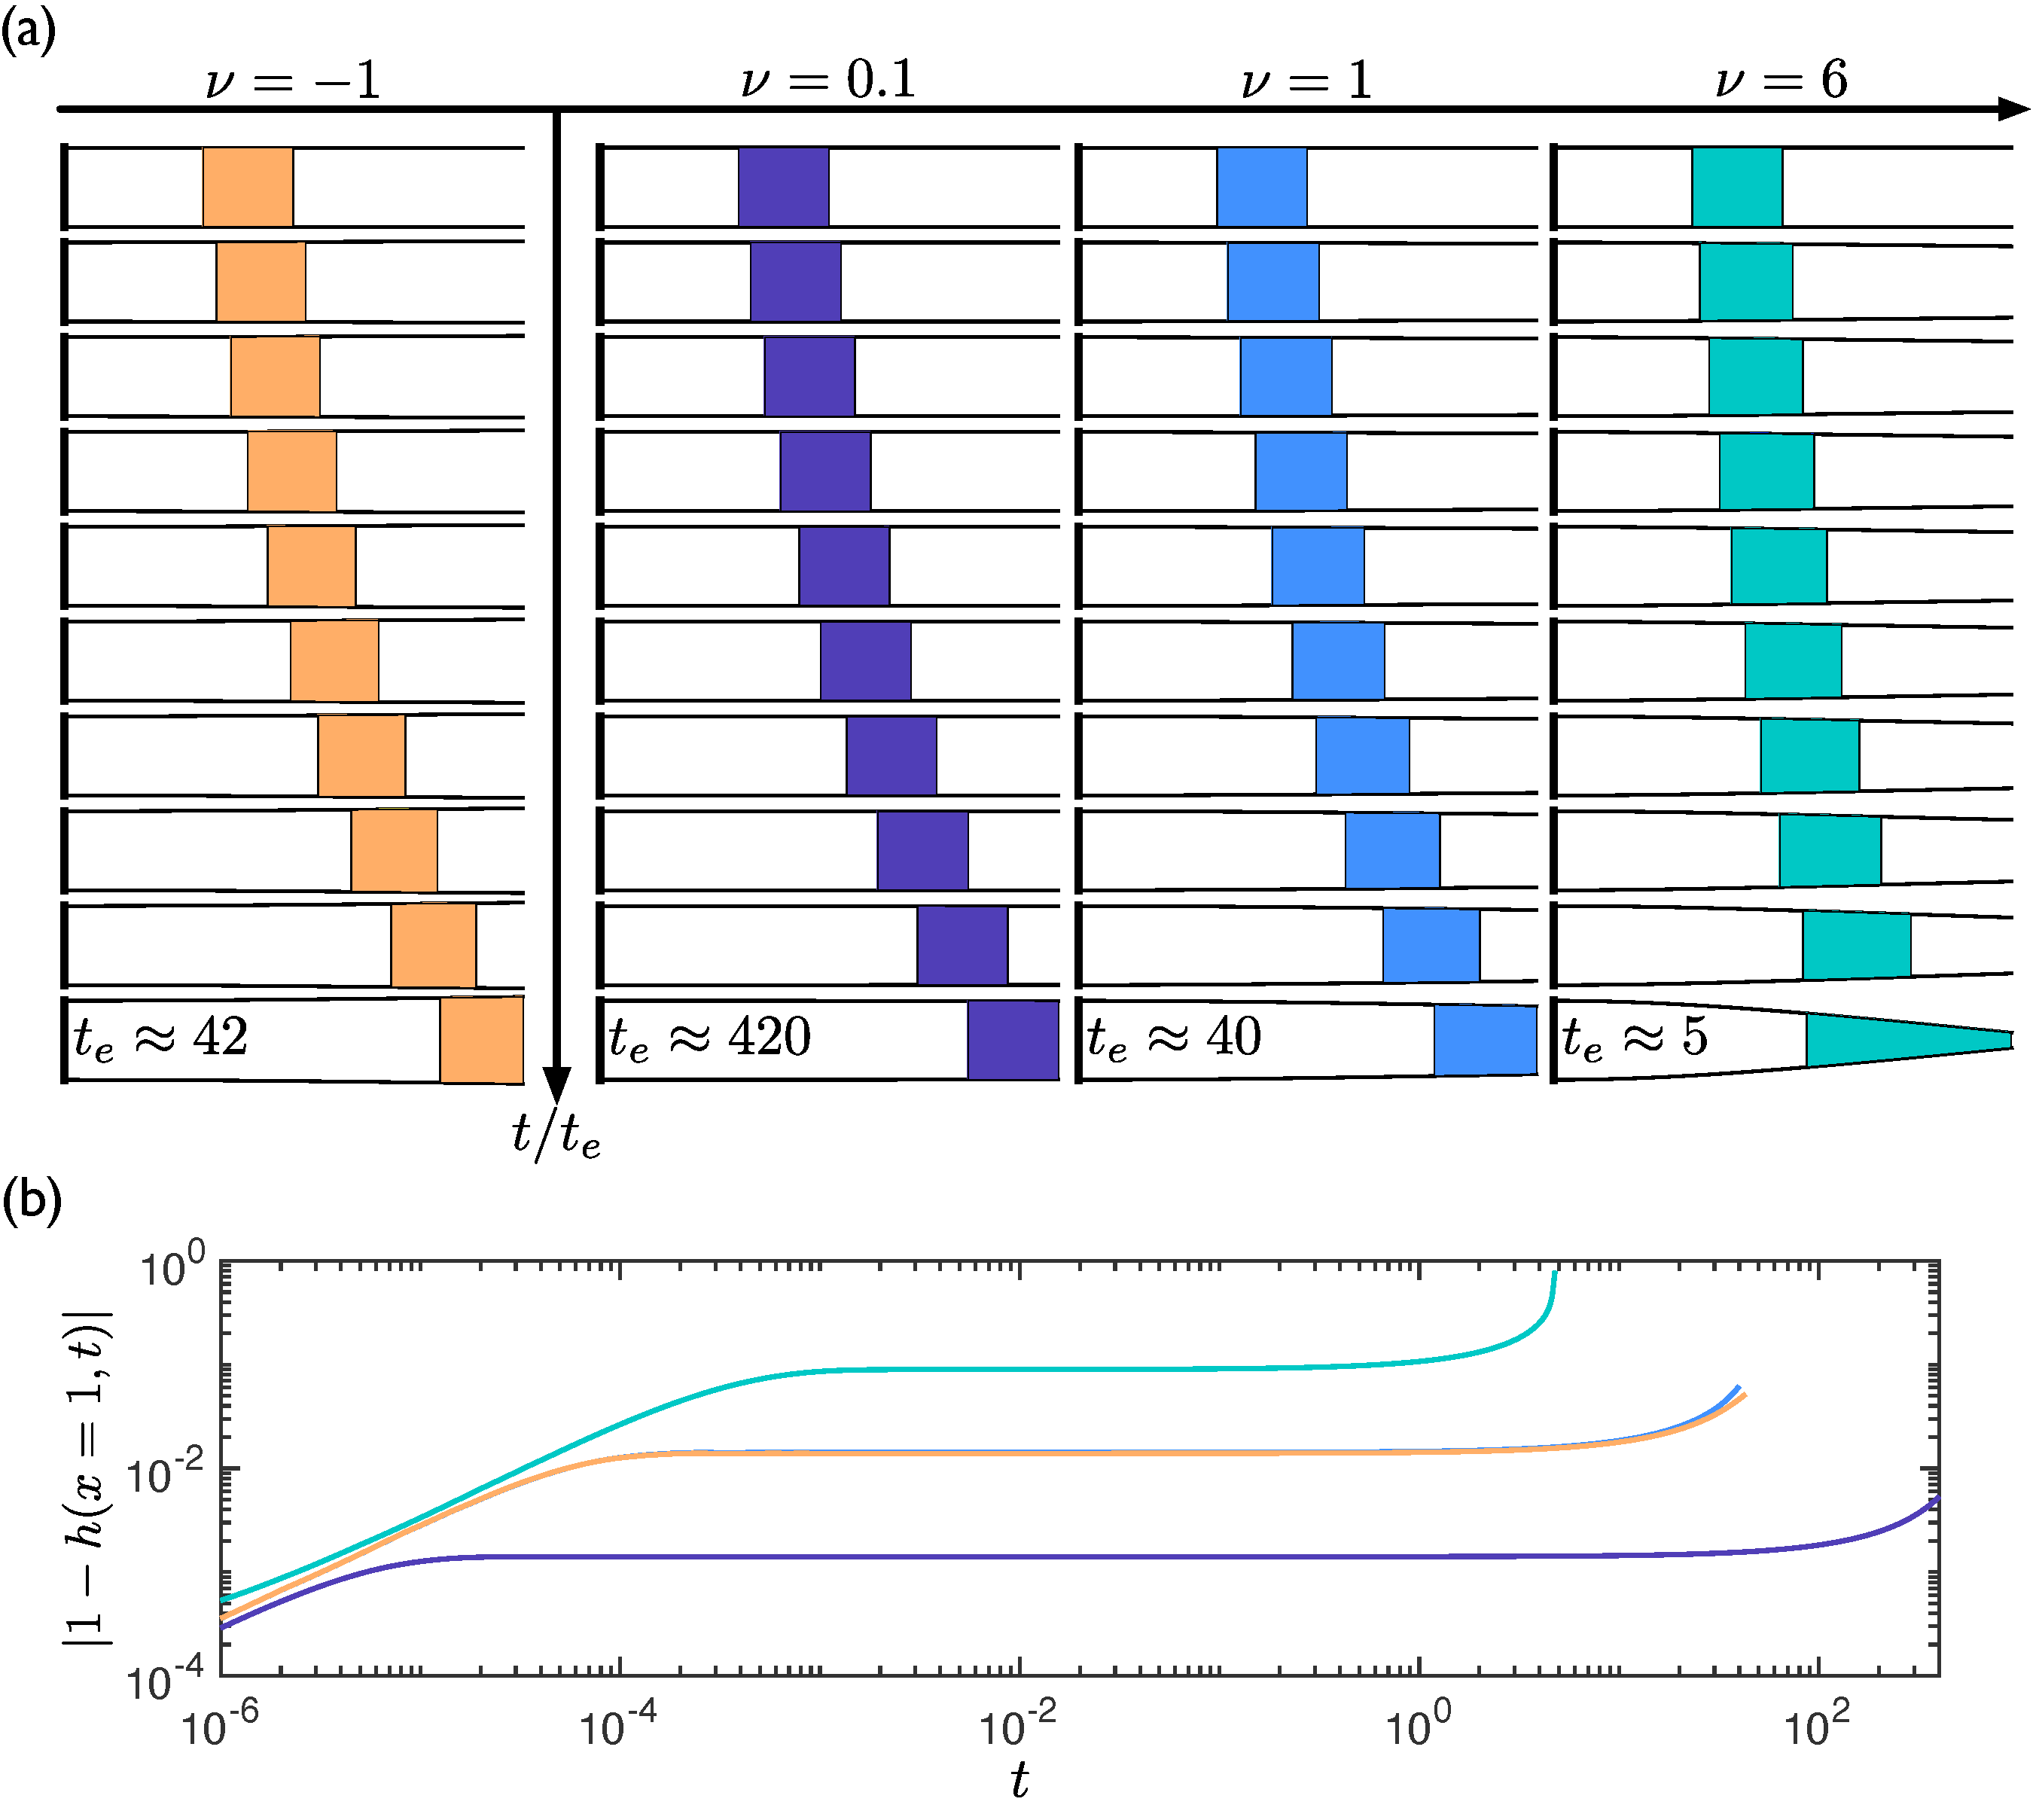
\includegraphics[width = 0.95\textwidth]{Phenomenology}
\caption{(a) Droplet-channel configurations obtained from numerical solutions of the model equations~\eqref{E:Chapter2:Model:NonDim:CombinedEq1}--\eqref{E:Chapter2:Model:NonDim:CombinedEq3},~\eqref{E:Chapter2:Model:NonDim:Kinematic}--\eqref{E:Chapter2:Model:NonDim:IC}.  The initial conditions -- $\xright^0 = 0.5, \xleft^0 = 0.3$ (giving $V = 0.2$) -- are the same for each value of $\nu$ shown. Snapshots vary linearly from $t/t_e = 0$ (top row) to $t/t_e = 1$ (bottom row), where $t_e$ denotes the time at which the droplet reaches the free end. (b) Displacement of the channel tip away from its initial position in the solutions shown in (a), with colours corresponding to those in (a). The three wetting configurations ($\nu = 0.1, 1,6$) have $h(1,t)<1$ (indicating inwards wall deflections), while the non-wetting configuration ($\nu = -1$) has $ h(1,t)>1$ (outwards deflections, respectively).}
\label{fig:Chapter2:Numerics:NumericalExperiments:Phenomenology}
\end{figure}
Schematic plots of numerical solutions of the model equations are shown in Figure~\ref{fig:Chapter2:Numerics:NumericalExperiments:Phenomenology}. The behaviour seen in these solutions span that seen in all numerical solutions; in this section, we briefly describe their features.

The salient feature of these solutions is that droplets are transported to the free end in both wetting ($\nu > 0$) and non-wetting ($\nu < 0$) scenarios, confirming that our model captures the wettability-independent nature of bendotaxis (Figure~\ref{fig:Chapter2:Numerics:NumericalExperiments:Phenomenology}(a)). Further, this droplet transport is accompanied by an inwards (outwards) deflection for wetting (non-wetting, respectively) configurations, as we predicted in our discussion of the mechanism in \S1.4.2.

In all cases, there is a qualitative similarity between the droplet trajectories, albeit on vastly different time scales (as we shall see, the droplet trajectory can be described analytically in the case of small deflections). In the proof of concept experiment, described in \S1.4.3, where $\nu = 5, \tau_c = 10$, the droplet took $\mathcal{O}(1~\text{minute})$ to traverse the channel. This is in qualitative agreement with the model result for $\nu = 6$, which predicts that the motion to takes approximately $5\tau_c$ seconds. Additionally, in the experiment, the droplet accelerates along the channel, which is in qualitative agreement with the shape of the droplet trajectories (Figure~\ref{fig:Chapter2:Numerics:NumericalExperiments:Phenomenology}(a)). (In the following chapter we describe a suite of detailed experiments designed to test the assumptions of our model -- especially the lubrication approximation within the droplet -- more closely.)

Stronger surface tension (larger $\nu$) is associated with larger deflections (Figure~\ref{fig:Chapter2:Numerics:NumericalExperiments:Phenomenology}(b)). As predicted, when surface tension is relatively strong, and the liquid wets the channel walls ($\nu = 6$ case in Figure~\ref{fig:Chapter2:Numerics:NumericalExperiments:Phenomenology}), the beam ends approach one another during the motion. As a result, the droplet spreads out, occupying a greater portion of the  length of the channel. Note that the value of $\nu = 6$ is (approximately) the largest $\nu$ for which the channel walls do not touch before the droplet reaches $\xright = 1$ (for this particular pair of initial conditions $(\xleft^0, \xright^0)$); if $\nu  \gtrsim 6$, the simulation ends before the droplet reaches $\xright = 1$, when the channel walls touch (we shall discuss what happens beyond this point in Chapter 4).

Recent studies of bendo-capillary imbibition from a bath of liquid~\citep{vanHonschoten2007JApplPhys,Aristoff2011IntJNonlinMech} have shown that the leading meniscus decelerates throughout the motion. By contrast, we observe here that droplets accelerate as they move along the channel (Figure~\ref{fig:Chapter2:Numerics:NumericalExperiments:Phenomenology}(a)). This acceleration occurs because the channel becomes more deformable the further the droplet is from the clamped end.

In the imbibition case, there is no rear meniscus, and the pressure gradient acts over a length equal to the leading meniscus position. Although meniscus advance results in a decrease in pressure at the front -- arising from additional channel deflection -- this does not overcome the additional length over which this pressure difference acts. (Note that bendo-capillary imbibition from a fixed bath is only possible for wetting configurations). In the case of bendotaxis, however, the rear meniscus is mobile, and the length over which the pressure gradient acts does not change significantly (Figure~\ref{fig:Chapter2:Numerics:NumericalExperiments:Phenomenology}(a)), allowing the increased effective deformability of the channel to dominate.

A comparison of the displacement of the channel tip from its initial position (Figure~\ref{fig:Chapter2:Numerics:NumericalExperiments:Phenomenology}(b)) suggests that the dynamic behaviour occurs on two distinct time scales: a fast, early time scale -- arising from a torque imbalance on the channel walls (the initially undeformed walls offer no resistance), and a slower time scale on which the droplets move. (This separation of time scales can be formalised in the case of small deflections.)

We also note the similarity between the tip displacement traces (Figure~\ref{fig:Chapter2:Numerics:NumericalExperiments:Phenomenology}(b)) for $\nu = \pm1$. For the majority of the motion, the deflection in these cases is relatively small, so the linearized form of the model equations are valid; as we shall see, the tip displacement and meniscus positions are symmetric in $\nu \to -\nu$ in solutions of the linearized equations. Only when deflections are significant, and non-linearities arising from the channel permeability, meniscus pressure, and conservation of mass enter, do the traces deviate from one another.  This again highlights the importance of the small deflection regime, which we turn to now.

\section{Small deflections}\label{S:Ch2:SmallDeformations}
We seek to make analytical progress by assuming that the deflections of the channel are small. Physically, small deflections are associated with weak surface tension or stiff channel walls; in our model, these two cases can be encoded by considering
\begin{equation}\label{E:Chapter2:SmallDef:Limit}
\bendability = \frac{\gamma \cos \theta_e L^4 }{B H^2} \ll 1.
\end{equation}
In this section, we therefore perform an asymptotic analysis of the model equations in the limit $\bendability \to 0$. (Note that small deflections can be also be realised by considering a small droplet volume, $V \ll 1$; we present an asymptotic analysis for $V \ll 1$  in Appendix~\ref{A:Ch2:SmallDroplets}.)

\subsection{Asymptotic expansion}
To probe the structure of  weak deviations from an undeformed configuration, $h(x,t) = 1$, we pose an expansion of the channel width in powers of $\bendability$:
\begin{equation}\label{E:Chapter2:SmallDef:Expansion}
h(x,t) = 1 + \bendability h_1(x,t) + \bendability^2 h_2(x,t) + \dots,
\end{equation}
where $h_i = \mathcal{O}(1)$ as $\bendability \to 0$.  Inserting~\eqref{E:Chapter2:SmallDef:Expansion} into the drop-only formulation of the problem problem (equations~\eqref{E:Chapter2:Numerics:SchemE:Chapter2:Reduced:EffectiveBCLower},~\eqref{E:Chapter2:Numerics:SchemE:Chapter2:Reduced:EffectiveBCUpper}--\eqref{E:Chapter2:Numerics:SchemE:Chapter2:Reduced:ReducedProblemIC}) and expanding in powers of $\bendability$ gives the PDE on the drop region as
\begin{equation}\label{E:Chapter2:SmallDef:PDE}
3|\bendability|\ddp{h_1}{t} =  \ddp{^6 h_1}{x^6} + \bendability \ddp{}{x}\left(3h_1 \ddp{^5 h_1}{x^5} + \ddp{^5 h_2}{x^5}\right),  \quad \xleft < x < \xright,
\end{equation}
correct to $\mathcal{O}(\bendability^2)$. The boundary and kinematic conditions, also correct to $\mathcal{O}(\bendability^2)$, are
\begin{align}
\ddp{^2 h_1}{x^2} - \frac{2}{\xleft^2}\left(2\xleft \ddp{h_1}{x} - 3h_1\right) + \bendability\left[ \ddp{^2 h_2}{x^2} - \frac{2}{\xleft^2}\left(2\xleft \ddp{h_2}{x} - 3h_2\right) \right] &= 0,\label{E:Chapter2:SmallDef:BC1}\\
\ddp{^3 h_1}{x^3} - \frac{6}{\xleft^3}\left(\xleft \ddp{h_1}{x} - 2h_1\right) + \bendability\left[ \ddp{^3 h_2}{x^3} - \frac{6}{\xleft^3}\left(\xleft \ddp{h_2}{x} - 2h_2\right) \right] &= 0,\label{E:Chapter2:SmallDef:BC2}\\
\ddp{^4 h_1}{x^4} + 1 + \bendability \left(\ddp{^4 h_2}{x^4} - h_1\right) &=0\label{E:Chapter2:SmallDef:BC3}
\end{align}
at $x = \xleft$,  and
\begin{align}
\ddp{^2 h_1}{x^2} + \bendability \ddp{^2 h_2}{x^2} &=0,\label{E:Chapter2:SmallDef:BC4}\\
\ddp{^3 h_1}{x^3} + \bendability \ddp{^3 h_2}{x^3} &=0,\label{E:Chapter2:SmallDef:BC5}\\
\ddp{^4 h_1}{x^4} + 1 + \bendability \left(\ddp{^4 h_2}{x^4} - h_1\right)&=0,\label{E:Chapter2:SmallDef:BC6}
\end{align}
at $x = \xright$, and
\begin{equation}\label{E:Chapter2:SmallDef:Kinematic}
3\mathrm{sgn}(\bendability) \ddp{x_{\pm}}{t} =\left. \left[  \ddp{^5 h_1}{x^5}  + \bendability \left(2 h_1 \ddp{^5 h_1}{x^5} +\ddp{^5 h_2}{x^5}\right)\right]\right|_{x = x_{\pm}}.
\end{equation}
Here $\mathrm{sgn}$ is the signum function, returning $1$ for $\nu > 0$ and $-1$ for $\nu < 0$, which arises from $\nu/|\nu| = \mathrm{sgn}(\nu)$.
\subsection{Separation of time scales}
The hierarchy of problems resulting from the asymptotic expansion sheds light on the different time scales alluded to earlier in \S\ref{S:Ch2:Numerics:Experiments}. We discuss these time scales briefly here.

By comparing the first term on the left hand side of~\eqref{E:Chapter2:SmallDef:PDE} with the first term on the right hand side, we identify a balance between channel squeezing and flux divergence on a fast ($\mathcal{O}(|\bendability|)$) time scale. Explicitly, if $T = t/|\bendability| \sim \mathcal{O}(1)$, the leading order equation in~\eqref{E:Chapter2:SmallDef:PDE} reads
\begin{equation}\label{E:Chapter2:SmallDef:TimeScales:FastPDE}
3\ddp{h_1}{T} = \ddp{^6 h_1}{x^6},
\end{equation}
and~\eqref{E:Chapter2:SmallDef:Kinematic} reads
\begin{equation}\label{E:Chapter2:SmallDef:TimeScales:FastKBC}
\ddp{x_{\pm}}{T} = \mathcal{O}(\bendability),
\end{equation}
i.e.~droplets do not move appreciably on this fast time scale. Equations~\eqref{E:Chapter2:SmallDef:TimeScales:FastPDE} and~\eqref{E:Chapter2:SmallDef:TimeScales:FastKBC} describe how the (initially straight) channel walls respond quickly to the non-zero droplet pressure by bending; this deflection induces a restoring force within the beams to balance the droplet pressure. The menisci move an $\mathcal{O}(\bendability)$ amount during this motion (in opposite directions because mass must be conserved), which is small in comparison with the total length of the channel. As it provides no information about the droplet motion, we do not pursue the problem on this time scale further.

It appears, from~\eqref{E:Chapter2:SmallDef:Kinematic}, that there is a balance between droplet motion and the leading order pressure gradient, $\partial^5 h_1/ \partial x^5$, on an $\mathcal{O}(1)$ time scale. From~\eqref{E:Chapter2:SmallDef:PDE}, we see that the leading order pressure gradient is quasistatic on this time scale: $\partial^5 h_1/ \partial x^5$ is a function of time only,  and hence the leading order pressure simply interpolates between its values at the two menisci. However, from~\eqref{E:Chapter2:SmallDef:BC3} and~\eqref{E:Chapter2:SmallDef:BC6}, these mensicus pressures are identical. Therefore the leading order pressure gradient is zero and the droplet does not move appreciably on an $\mathcal{O}(1)$ time scale either. As we shall see, the droplet moves on a long ($\mathcal{O}(|\bendability|^{-1})$) time scale; the large difference in the magnitude of this long time scale, and the short time scale on which the channel initially responds to applied pressure can be seen in our numerical solutions (see Figure~\ref{fig:Chapter2:Numerics:NumericalExperiments:Phenomenology}(b), for example).

\subsection{Droplet motion time scale}
To analyse the problem on the time scale of droplet motion, we rescale time by introducing $\tau = 3|\bendability| t \sim \mathcal{O}(1)$.  The PDE for $h_1(x,\tau)$ is
\begin{equation}\label{E:Chapter2:SmallDef:SlowTimescale:PDE}
\ddp{^6h_1}{x^6} = 0 \qquad \xleft(\tau) < x <\xright(\tau).
\end{equation}
The boundary conditions
\begin{equation}\label{E:Chapter2:SmallDef:SlowTimescale:BC1}
\ddp{^2 h_1}{x^2} - \frac{2}{\xleft^2}\left(2\xleft \ddp{h_1}{x} - 3h_1\right)= 0 = \ddp{^3 h_1}{x^3} - \frac{6}{\xleft^3}\left(\xleft \ddp{h_1}{x} - 2h_1\right) \quad \text{at}~x = \xleft,
\end{equation}
\begin{equation}\label{E:Chapter2:SmallDef:SlowTimescale:BC2}
\ddp{^2 h_1}{x^2} = 0 = \ddp{^3 h_1}{x^3}  \quad \text{at}~x = \xright, \qquad  \ddp{^4 h_1}{x^4}  = -1 \quad \text{at}~x = x_{\pm}
\end{equation}
are unaffected by the time scaling (and hence the problem for $h_1(x,\tau)$ is identical to that for $h_1(x,t)$).

The solution to~\eqref{E:Chapter2:SmallDef:SlowTimescale:PDE}--\eqref{E:Chapter2:SmallDef:SlowTimescale:BC2} is
%\begin{equation}\label{E:Chapter2:SmallDef:SlowTimescale:Solution}
%h_1(x,\tau) =-  \frac{1}{24}\left[(\xright- x)^4 - 4(\xright^3 - \xleft^3)(\xright -x) + (3\xright^4 + \xleft^4 - 4\xright \xleft^3)\right]
%\end{equation}
%\blue{equivalent and probably nicer}
%\begin{multline}\label{E:Chapter2:SmallDef:SlowTimescale:Solution}
%h_1(x,\tau) =-  \frac{\xright^4}{24}\left\{\left(1- \frac{x}{\xright}\right)^4 - 4\left[1 - \left(\frac{\xleft}{\xright}\right)^3\right]\left(1 -\frac{x}{\xright}\right) +\right.\\\left. \left[3 +\left(\frac{\xleft}{\xright}\right)^4 - 4 \left(\frac{\xleft}{\xright}\right)^3\right]\right\}
%\end{multline}
%\blue{maybe even nicer?}
\begin{equation}\label{E:Chapter2:SmallDef:SlowTimescale:Solution}
h_1(x,\tau) =-  \frac{\xright^4}{24}\left[\left(1-\xi\right)^4 - 4(1 - \xi_m^3)(1 -\xi) + (3 +\xi_m^4 - 4 \xi_m^3)\right]
\end{equation}
where $\xi(x, \tau) = x/\xright(\tau)$ and $\xi_m(\tau) = \xleft(\tau) /\xright(\tau)$. Although the deflection~\eqref{E:Chapter2:SmallDef:SlowTimescale:Solution} does not contribute to the meniscus motion (as discussed, it corresponds to a uniform pressure), it is necessary to solve for $h_1$  to determine $h_2(x, \tau)$ and thus the droplet motion via the kinematic boundary condition, which reads
\begin{equation}\label{E:Chapter2:SmallDef:SlowTimescale:Kinematic}
\dd{x_{\pm}}{\tau} = -\left.\ddp{^5 h_2}{x^5}\right|_{x = x_\pm(\tau)},
\end{equation}
at leading order.

The problem for $h_2(x, \tau)$ is also quasi-static:
\begin{equation}\label{E:Chapter2:SmallDef:SlowTimescale:PDE_firstorder}
\ddp{^6h_2}{x^6} = 0 \qquad \xleft(\tau) < x <\xright(\tau),
\end{equation}
with boundary conditions
\begin{equation}\label{E:Chapter2:SmallDef:SlowTimescale:firstorder_BC1}
\ddp{^2 h_2}{x^2} - \frac{2}{\xleft^2}\left(2\xleft \ddp{h_2}{x} - 3h_2\right)= 0 = \ddp{^3 h_2}{x^3} - \frac{6}{\xleft^3}\left(\xleft \ddp{h_2}{x} - 2h_2\right) \quad \text{at}~x = \xleft,
\end{equation}
\abeqn{E:Chapter2:SmallDef:SlowTimescale:firstorder_BC2}{\ddp{^2 h_2}{x^2} = 0 = \ddp{^3 h_2}{x^3}  \quad \text{at}~x = \xright, \qquad  \ddp{^4 h_2}{x^4}  =  h_1 \quad \text{at}~x = x_{\pm}.}
Note that the only inhomogeneity in the $h_2$ problem comes via the forcing in the pressure at $x_{\pm}$ (i.e.~through~\eqref{E:Chapter2:SmallDef:SlowTimescale:firstorder_BC2}b).

From~\eqref{E:Chapter2:SmallDef:SlowTimescale:PDE_firstorder}, we see that the pressure gradient is spatially independent, and thus set by the pressure difference across the droplet:
\begin{equation}
\ddp{^5 h_2}{x^5} = \frac{h_1(\xright,\tau) - h_1(\xleft, \tau)}{\xright - \xleft} =-\frac{\xright(\tau)^3}{8}\left[1-\xi_m(\tau)\right]\left[1+\xi_m(\tau)\right]^2.
\end{equation}
Here we have used the solution~\eqref{E:Chapter2:SmallDef:SlowTimescale:Solution} to evaluate $h_1(x_\pm,t)$. It is then clear from the kinematic condition~\eqref{E:Chapter2:SmallDef:SlowTimescale:Kinematic} that both menisci move at the same speed,
\begin{equation}\label{E:Chapter2:SmallDef:SlowTimescale:ODE}
\dd{x_{\pm}}{\tau}  = \frac{\xright^3}{8}(1-\xi_m)(1+\xi_m)^2 = \frac{(\xright - \xleft)(\xright + \xleft)^2}{8}
\end{equation}
and hence the drop length $\xright - \xleft$ does not change at leading order during the motion. Since the menisci do not move appreciably on the faster time scales discussed above (recall that on an $\mathcal{O}(|\bendability|^{-1})$ time scale the menisci move an $\mathcal{O}(\bendability)$ amount), the droplet length stays at its initial value, $\xright - \xleft\approx  \xright^0 - \xleft^0 = V$ and thus $\xright + \xleft \approx 2\xright - V$.

Using this, the solution to~\eqref{E:Chapter2:SmallDef:SlowTimescale:ODE} with initial condition $\xright(\tau = 0) =\xright(t = 0) = \xright^0$, is, in terms of the original (unscaled) dimensionless variables,
\begin{equation}\label{E:Chapter2:SmallDef:SlowTimescale:xright_original_variables}
\xright(t) = \frac{V}{2}\left[1 + \left(\frac{V}{2\xright^0 - V} - \frac{3V^2 |\bendability | t}{4}\right)^{-1}\right] + \mathcal{O}(|\bendability|^2),
\end{equation}
with $\xleft = \xright - V + \mathcal{O}(|\bendability|)$. Note that  this expression is symmetric in $\nu \rightarrow -\nu$: droplets in channels with the same absolute bendability, but with different wettability conditions, travel at the same speed when the channel deflections are small, as observed in numerical solutions presented in \S\ref{S:Ch2:Numerics:Experiments}.


\begin{figure}[th]
\centering
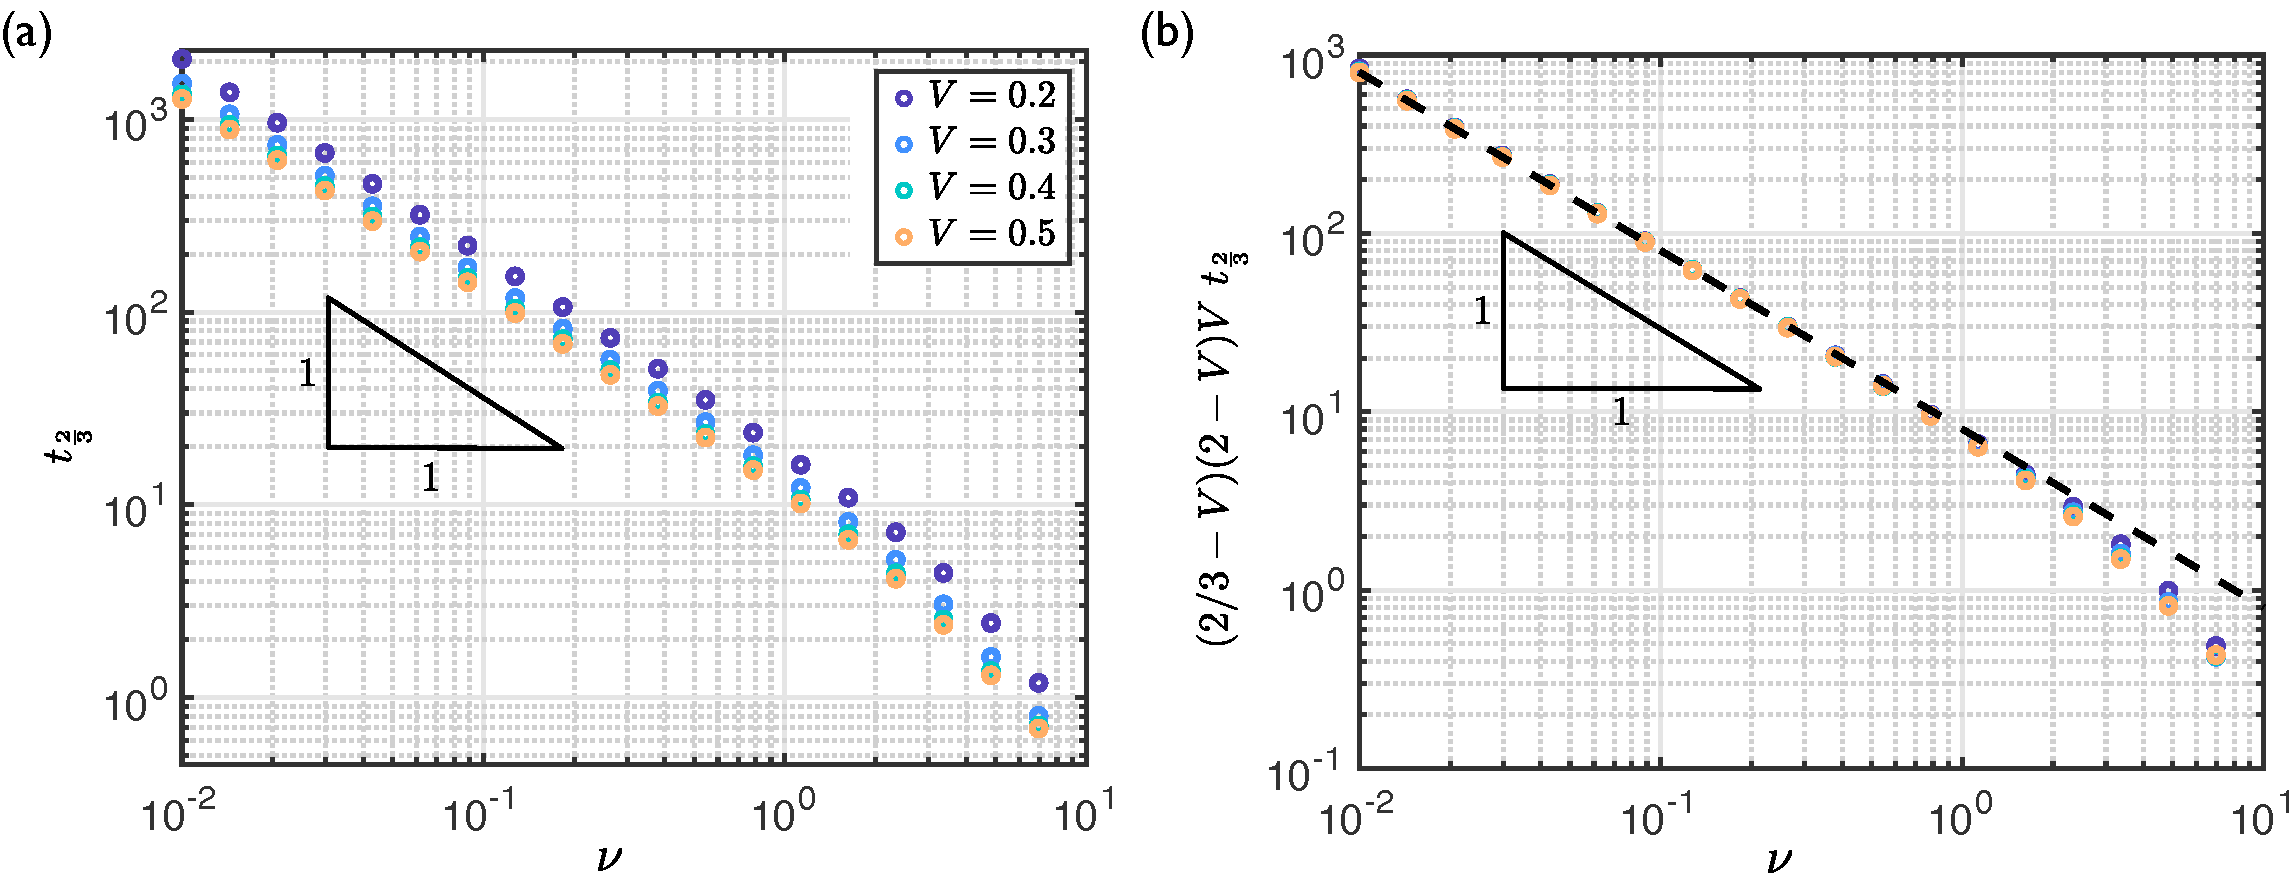
\includegraphics[width = \textwidth]{Asymptotics}
\caption{(a) Numerically obtained values of $t_{2/3}$ (the time taken for the droplet to traverse the last 1/3\textsuperscript{rd} on the channel) plotted on logarithmic axes. The colour of points indicates the relative volume $V$ (see legend in (a)). (b) Data in (a) rescaled according to the asymptotic prediction~\eqref{E:Chapter2:SmallDef:SlowTimescale:AsymptoticTf}. The dashed black line indicates $t_{2/3} = t_{2/3}^{\text{SB}}$, the asymptotic result in the case of small deflections.}
\label{fig:Chapter2:SmallDeformations:Asymptotics}
\end{figure}

As a proxy for the time scale of motion, we consider $t_f$ -- the time taken for the leading meniscus to pass from $\xright = f < 1$ to the free end, $\xright = 1$. As $t_f$ is the time \emph{difference} between two events, the system is free of inertia, and the capillary torque is balanced by beam bending (except for at early times, when the droplet does not move significantly), we expect $t_f$ to be approximately independent of the initial conditions. This allows us to consider the dynamic behaviour only in terms of the control parameters of interest: $\bendability$ and $V$. (As we shall see, $t_f$, rather than the total time for the motion, is the relevant observable  in our experimental study of bendotaxis.)

Using the solution~\eqref{E:Chapter2:SmallDef:SlowTimescale:xright_original_variables}, we find that the small bendability estimate of $t_f$, denoted $t_f^\text{SB}$, is
\begin{equation}\label{E:Chapter2:SmallDef:SlowTimescale:AsymptoticTf}
t_f^{\text{SB}} = \frac{24(1 - f)}{(2f - V)(2 - V)}\frac{1}{|\nu| V},
\end{equation}
Noting that
\begin{equation}\label{E:Chapter2:SmallDef:SlowTimescale:ComparisonToScaling}
\frac{1}{\nu V} =  \frac{B H^2}{|\gamma \cos \theta_e| L^4}\frac{L}{\Delta X}  =  \frac{B}{|\gamma \cos \theta_e| \Delta X}\frac{H^2}{L^3},
\end{equation}
the result~\eqref{E:Chapter2:SmallDef:SlowTimescale:AsymptoticTf} is in agreement with the result of the scaling argument presented in \S\ref{S:Model:Scaling}, namely equation~\eqref{E:Chapter2:Model:Scaling:ScalingResult}.

Numerical solutions of the full problem with $\nu \ll 1$ agree well with~\eqref{E:Chapter2:SmallDef:SlowTimescale:AsymptoticTf} (Figure~\ref{fig:Chapter2:SmallDeformations:Asymptotics}). These results are shown for $t = t_f$ with $f = 2/3$ (in which case $t_f$ is the time taken to traverse the final 1/3\textsuperscript{rd} of the channel). Surprisingly, the expression~\eqref{E:Chapter2:SmallDef:SlowTimescale:AsymptoticTf} accurately predicts $t_f$ in numerical solutions even when $\nu = \mathcal{O}(1)$, and the asymptotic analysis is no longer valid.

To understand this, we consider the dynamics in the limit of small droplets ($V \ll 1$): in Appendix~\ref{A:Ch2:SmallDroplets}, we show that the corresponding small droplet result for $t_f$ is
\begin{equation}\label{E:Chapter2:SmallDef:SlowTimescale:AsymptoticTfSmallVolume} t_f^{\text{SV}} = \frac{6(1 - f)}{f}\frac{1}{|\nu| V},
\end{equation}
Note that
\begin{equation}
\frac{24(1 - f)}{(2f - V)(2 - V)} =  \frac{6(1 - f)}{f}\left[1 + \frac{V^2}{4f} + \mathcal{O}(V)\right],
\end{equation}
i.e.~$t_f^{\text{SB}} = t_f^{\text{SV}} + \mathcal{O}(V)$. The agreement between numerical solutions and~\eqref{E:Chapter2:SmallDef:SlowTimescale:AsymptoticTf}  for $\nu = \mathcal{O}(1)$ (Figure~\ref{fig:Chapter2:SmallDeformations:Asymptotics}) in fact reflects agreement with the result~\eqref{E:Chapter2:SmallDef:SlowTimescale:AsymptoticTfSmallVolume} for small volumes. As mentioned, both the cases of small bendability (and $V \lesssim \mathcal{O}(1)$) and small droplet volume (and $\nu \lesssim \mathcal{O}(1)$) will result in a small channel deflections, but the asymptotic analysis of this section is only valid in the case of the former. Note that, the larger $V$ is, the sooner the data from numerical solutions `peel off' from the asymptotic result~\eqref{E:Chapter2:SmallDef:SlowTimescale:AsymptoticTf}~(Figure~\ref{fig:Chapter2:SmallDeformations:Asymptotics}(b)). It is difficult to separate the two small deflections cases -- small bendability and small droplet volume -- since droplets have $V < 1$ by construction (and we are typically interested in $V < 1/2$).


\section{Droplet removal}
\begin{figure}
\centering
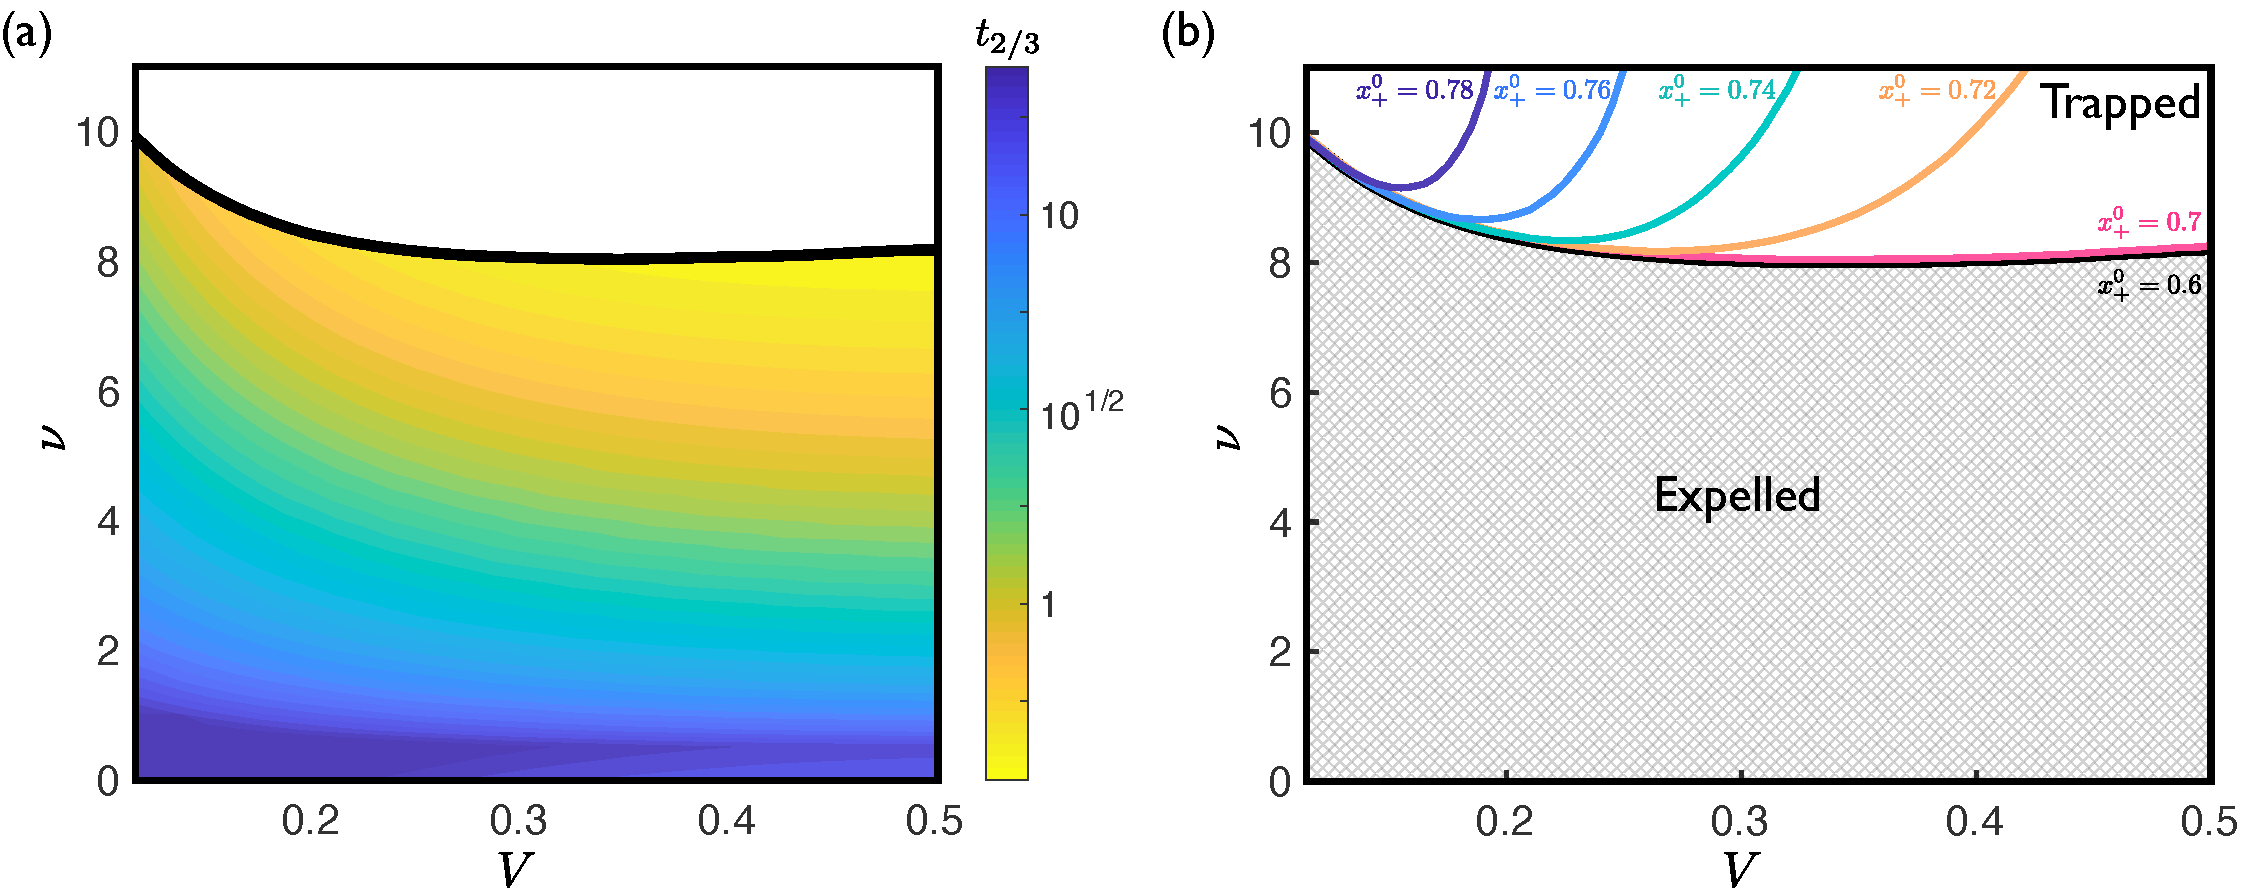
\includegraphics[width = 0.95\textwidth]{optimal_removal_split}
\caption{(a) Influence of dimensionless droplet volume $V$ and channel bendability $\nu$ on numerically obtained values of $t_{2/3}$ (the time taken to traverse the final 1/3\textsuperscript{rd} of the channel) with $\xright^0 = 0.6$. The solid black line indicates indicates $\nu_c(V,\xright^0 = 0.6)$, the smallest value of $\nu$ (for a given $V$) in which the channel walls touch before the droplet reaches the free end. (b) Numerically obtained values of $\nu_c(V,\xright^0)$ for different initial droplet positions $\xright^0$. Droplets are always expelled (reach the free end) for $\nu < \nu_c$, and trapped (the channel walls touch before the droplet reaches the free end) for $\nu > \nu_c$ (the hatched region indicates the expelled region for $\xright^0 \lesssim 0.7$).}
\label{fig:Ch2:DropRemoval}
\end{figure}
We conclude this chapter with a brief discussion of the implications of our model for droplet removal from deformable channels --  our main motivation for studying bendotaxis. In particular, we consider the time taken for a droplet to reach the free end (from which it can be removed). This quantity is important because the overall performance of the structure is strongly dependent on the number of compromised channels -- those containing a droplet. Increasing the speed of removal from individual channels will minimise the total number of compromised channels.

A key question is, therefore, how should a channel be designed to minimize the time taken for droplets to reach the free end? In answering this question, we again consider $t_f$, rather than the total time taken, to isolate the effects of the bendability $\nu$ and droplet volume $V$.

We solve the model equations presented in \S\ref{S:Chapter2:Model:NonDim} numerically for a variety of $(V, \nu)$ pairs to map $t_f$ as a function of $\nu$ and $V$ (Figure~\ref{fig:Ch2:DropRemoval}(a)). This map confirms the trend suggested by those numerical solutions shown in Figure~\ref{fig:Chapter2:Numerics:NumericalExperiments:Phenomenology}: increasing the  bendability, $\nu = \gamma \cos \theta_e L^4/(BH^2)$, reduces the time taken for the droplets to traverse a section of the channel adjacent to the free end. However, this is to be weighed against the possibility that the walls touch during the motion and trap (wetting) drops indefinitely. The regions of $(V, \nu)$ space for which the droplet is ultimately trapped or reaches the free end is shown in Figure~\ref{fig:Ch2:DropRemoval}(b). %some m ention of (a) how this is acheived in practice (e.g. lengthening channel), (b) the hidden L^2/H_0 in the time scale?

We denote by $\nu_c(V,\xright^0)$ the smallest value of $\nu$ at which the channel walls touch -- and trap the drop -- during the motion (before $t = t_e$, when the simulation ends), for a given  droplet volume $V$ and initial position $\xright^0$, i.e.
\begin{equation}
\nu_c = \sup\left\{\nu | h(x = 1, t = t_e) > 0\right\}.
\end{equation}
(This supremum is well defined because $h(x = 1, t = t_e)$ is a decreasing function of $\nu$ for a given $(V, \xright)$.) We compute $\nu_c$ numerically using a bisection scheme. Each evaluation of $h(x = 1, t = t_{e})$ requires us to solve the model equations numerically for $t \leq t_e$.

We plot in Figure~\ref{fig:Ch2:DropRemoval}(b) the curves $\nu_c$ as a function of $V$, for various $\xright^0$.These curves are approximately independent of $\xright^0$ when $\xright^0 \lesssim 0.7$, but are very sensitive to $\xright$ when $\xright^0>0.7$ (i.e.~$\partial \nu_c /\partial \xright^0 \gg 1$ when $\xright^0>0.7$). To understand this we note that, provided the channel walls do not touch, the channel width at $x = 1$ depends only on the channel width and slope at $x = \xright$, and the (instantaneous) droplet position via the distance $1 - \xright$ between the channel end and the `$+$' meniscus (see equation~\eqref{E:Chapter2:Numerics:SchemE:Chapter2:Reduced:ShapeUpper}).  In general, the channel width and slope are set by an instantaneous torque balance on the beams, and the history of the droplet is unimportant. This torque balance is, however, not valid during the early squeezing regime: droplets starting close to the free end may be able to reach it during this period. For a given $V$, a stronger pull (larger $\nu$) is required to trap those droplets starting close to the free end.

\section{Summary}
In this section, we have developed a mathematical model of bendotaxis. The physics retained in our model is motivated by the experimental demonstration of bendotaxis presented in \S1.4.3. The model is characterized by three dimensionless parameters: a channel bendability (which implicitly describes the wettability conditions), a dimensionless droplet volume and a dimensionless starting position of the droplet.

Numerical solutions of the governing equations indicate that our model captures the wettability independent nature of bendotaxis, and its characteristic inwards deflections for wetting configurations and outwards deflection for non-wetting configurations. The numerical solutions predict motion on a time scale comparable to the experimental demonstration, with qualitatively similar dynamics. However, we have not made a detailed quantitative comparison between this experiment and the model; in the following chapter, we describe a suite of experiments similar to the proof of concept experiment which are designed to test the validity of our model.

We demonstrated how analytic progress can be made in quantifying the time scale of motion in the case of small deflections -- achieved by having either a small channel bendability or a small droplet volume. In both cases, the time scale of motion is inversely proportional to the product of the bendability and droplet volume, as was also predicted by a scaling argument. We also discussed the implications of our model for droplet removal from deformable channels; in particular, we identified that high channel bendability is desirable for quick droplet removal, but this this is to be weighed against the possibility of the tips of the channel walls touching and trapping wetting drops indefinitely. Finally, we note that for $\nu \lesssim 8$, droplets are always expelled, regardless of where the start in the channel; tailoring the surfaces design to ensure $\nu \lesssim 8$ may therefore be a good design criterion for superhydrophobic surfaces that exploit bendotaxis for anti-fogging.


%%%%%%%%%%%%%%%%%Appendices%%%%%%%%%%%%%%%
% uncomment below for thesis main compile
\begin{subappendices}
%\addcontentsline{toc}{section}{Appendices}
\renewcommand{\thesection}{\Alph{section}}
%\appendix
\section{Small droplets}\label{A:Ch2:SmallDroplets}
In this appendix, we consider the small volume droplets, $V \ll 1$. The aim is to derive a small volume approximation for $t_f$ -- the time taken between $\xright = f$ and $\xright = 1$ --  which we denote $t_f^{\text{SV}}$. Here we simply describe the leading order behaviour, as this is sufficient to determine $t_f^{\text{SV}}$ to leading order. %in constrast to the $\nu \ll 1$ case
\subsection{Small volume expansion}\label{A:Ch2:SmallDroplets:SmallVolumeExpansion}
We begin by assuming that the channel is not deflected significantly by the droplet, allowing us to write
\begin{equation}\label{A:E:Ch2:SmallDroplets:Expansion}
h(x,t) = 1 + Vh_1(x,t) + \mathcal{O}(V^2),
\end{equation}
where $h_1 \sim \mathcal{O}(1)$; as we shall see, enforcing this condition places a restriction on the range of $\nu$ allowed.

To begin, we first note that conservation of mass requires the length of the drop to remain small and approximately constant throughout the motion, $\xright - \xleft = V + \mathcal{O}(V^2)$.

Recall that the channel width in the drop region satisfies
\begin{equation}\label{A:E:Ch2:SmallDroplets:Reynolds}
\ddp{h}{t} = \frac{1}{3|\bendability|}\ddp{}{x}\left(h^3 \ddp{^5  h}{x^5}\right), \qquad \xleft < x <\xright.
\end{equation}
Inserting~\eqref{A:E:Ch2:SmallDroplets:Expansion} into~\eqref{A:E:Ch2:SmallDroplets:Reynolds} and integrating across the droplet gives
\begin{equation}\label{A:E:Ch2:SmallDroplets:IntegratedReynolds}
\left[h^3 \ddp{^5 h}{x^5}\right]_{\xleft}^{\xright} =3|\bendability| \int_{\xleft}^{\xright} V\ddp{h_1}{t}~\mathrm{d}x = \mathcal{O}(V^2),
\end{equation}
where the second equality makes use of the short length of the droplet. Equation~\eqref{A:E:Ch2:SmallDroplets:IntegratedReynolds} indicates that the liquid flux, which is proportional to $h^3 \partial^5h/\partial x^5$, does not vary significantly across the droplet. As a consequence, the pressure gradient is approximately (spatially) constant in the drop. Using the dimensionless Laplace pressure boundary condition~\eqref{E:Chapter2:Model:NonDim:BCPressure}, we can approximate this constant pressure gradient by
\begin{equation}\label{A:E:Ch2:SmallDroplets:DropPressureGradient}
\ddp{^5 h}{x^5} = \frac{1}{\xright - \xleft}\left[\ddp{^4 h}{x^4}\right]_{\xleft}^{\xright} + \mathcal{O}(V^2) =\frac{\nu}{\xright - \xleft}\left[\frac{1}{h(\xleft,t)} - \frac{1}{h(\xright,t)}\right] + \mathcal{O}(V^2).
\end{equation}
Now, by expanding the terms on the right hand side of~\eqref{A:E:Ch2:SmallDroplets:DropPressureGradient} as
\begin{equation}\label{A:E:Ch2:SmallDroplets:DropPressureChange}
\frac{1}{h(\xleft,t)} - \frac{1}{h(\xright,t)}  =V\left. \ddp{h}{x}\right|_{x = \xright} + \mathcal{O}(V^3) = \left.V^2 \ddp{h_1}{x}\right|_{x = \xright} + \mathcal{O}(V^3),
\end{equation}
we can express the pressure gradient as
\begin{equation}\label{A:E:Ch2:SmallDroplets:DropPressureGradient2}
\ddp{^5 h}{x^5} =\left. \nu V \ddp{h_1}{x}\right|_{x =\xright}+ \mathcal{O}(V^2),
\end{equation}
Inserting~\eqref{A:E:Ch2:SmallDroplets:DropPressureGradient2} into the kinematic condition~\eqref{E:Chapter2:Model:NonDim:Kinematic} gives (to leading order),
\begin{equation}\label{A:E:Ch2:SmallDroplets:ReducedKinematic}
\dd{\xright}{t} = -\left.\frac{\mathrm{sgn}(\nu)}{3} V\ddp{h_1}{x}\right|_{x =\xright}.
\end{equation}

\subsection{Point force problem}
To proceed, we require an estimate of the slope of the channel walls. Since the drop is small, its effect on the channel shape may be approximated by a point force acting at $x = \xright$; the channel `sees' the droplet only via jump conditions, which we derive by integrating the pressure across the droplet.

To begin, we note that, since the pressure gradient within the droplet is $\mathcal{O}(V)$ (equation~\eqref{A:E:Ch2:SmallDroplets:DropPressureGradient2}), the droplet pressure is approximately constant:
\begin{equation}\label{A:E:Ch2:SmallDroplets:DropPressure}
p(x,t) = \ddp{^4 h}{x^4} =  \left.\ddp{^4 h}{x^4}\right|_{x = \xright} + \mathcal{O}(V^2) = -\nu + \mathcal{O}(V^2)
\end{equation}
By integrating~\eqref{A:E:Ch2:SmallDroplets:DropPressure} across the droplet, we calculate the jump in shear force across it as
\begin{equation}\label{A:E:Ch2:SmallDroplets:ShearJump}
\left[\ddp{^3 h}{x^3}\right]_{\xleft}^{\xright} = -\nu V + \mathcal{O}(V^2).
\end{equation}
This is the first jump condition. The second jump condition comes from expanding the jump in channel shape across the droplet in $V$:
\begin{align}
\left[h\right]_{\xleft}^{\xright} &= h(\xright,t) - h(\xright - V,t)  \nonumber\\
&= 1 + V h_1(\xright,t) - \left[1 + V h_1(\xright - V,t)\right] + \mathcal{O}(V^2) \nonumber \\ &= 1 + V h_1(\xright,t) - \left[1 + V h_1(\xright,t)\right]+ \mathcal{O}(V^2)\nonumber \\&=  \mathcal{O}(V^2). \label{A:E:Ch2:SmallDroplets:ShapeSmall}
\end{align}

Similarly, by expanding the channel slope and moment, we obtain
\begin{equation}\label{A:E:Ch2:SmallDroplets:Slope_and_moment_small}
\left[\ddp{h}{x}\right]_{\xleft}^{\xright} = V\left.\ddp{^2 h}{x^2}\right|_{x = \xright} + \mathcal{O}(V^2), \qquad \left[\ddp{^2 h}{x^2}\right]_{\xleft}^{\xright} = V\left.\ddp{^3 h}{x^3}\right|_{x = \xright} + \mathcal{O}(V^2).
\end{equation}

Recall from \S\ref{S:Ch2:Numerics:Scheme:ReducedProblem} that the free boundary conditions applied at $x = 1$ also apply at $x = \xright$, i.e.
\begin{equation}\label{A:E:Ch2:SmallDroplets:EffFreeBC}{\left.\ddp{^2 h}{x^2}\right|_{x = \xright} = 0, \qquad \left.\ddp{^3 h}{x^3}\right|_{x = \xright} =0.}
\end{equation}
Combining~\eqref{A:E:Ch2:SmallDroplets:Slope_and_moment_small} and~\eqref{A:E:Ch2:SmallDroplets:EffFreeBC} yields the final two jump conditions
\begin{equation}\label{A:E:Ch2:SmallDroplets:Slope_and_moment_jump_conds}
\left[\ddp{h}{x}\right]_{\xleft}^{\xright} = \mathcal{O}(V^2), \qquad \left[\ddp{^2 h}{x^2}\right]_{\xleft}^{\xright} = \mathcal{O}(V^2).
\end{equation}

The leading order `point force problem' for $h_1$ is therefore
\begin{equation}\label{A:E:Ch2:SmallDroplets:PtForcePDE}
\ddp{^4 h_1}{x^4} = 0, \qquad \text{in}~0< x < \xright,~\text{and}~\xright < x < 1,
\end{equation}
with jump conditions
\begin{equation}\label{A:E:Ch2:SmallDroplets:PtForceJump}
\left[\ddp{^3 h_1}{x^3}\right]_{\xright^-}^{\xright^+} = -\nu, \qquad \left[\ddp{^2 h_1}{x^2}\right]_{\xright^-}^{\xright^+} =0, \qquad \left[\ddp{ h_1}{x}\right]_{\xright^-}^{\xright^+} =0,\qquad \left[h_1\right]_{\xright^-}^{\xright^+} = 0,
\end{equation}
and boundary conditions
\begin{align}
h_1 &= 0, \qquad  \ddp{h_1}{x}= 0, \qquad\text{at}~x = 0,\label{A:E:Ch2:SmallDroplets:PtForceBC1}\\
\dd{^2 h_1}{x^2} &= 0, \qquad \ddp{^3 h_1}{x^3}= 0, ~~\quad \text{at}~x = 1.\label{A:E:Ch2:SmallDroplets:PtForceBC2}
\end{align}
The solution to~\eqref{A:E:Ch2:SmallDroplets:PtForcePDE}--\eqref{A:E:Ch2:SmallDroplets:PtForceBC2} is
\begin{equation}\label{A:E:Ch2:SmallDroplets:SolutionShape}
h_1(x,t) = \begin{cases}{}
        -\frac{\bendability}{6}(3\xright x^2 - x^3) & \text{for }\quad 0 < x < \xright(t), \\
       -\frac{\bendability}{6}\left[3\xright^2(x - \xright) + 2 \xright^3\right] & \text{for }\quad \xright(t) < x < 1.
        \end{cases}
\end{equation}
This solution demonstrates that our assumption that $h_1\sim \mathcal{O}(1)$ is valid only when $\nu  \sim \mathcal{O}(1)$.

After inserting~\eqref{A:E:Ch2:SmallDroplets:SolutionShape} into the reduced kinematic condition~\eqref{A:E:Ch2:SmallDroplets:ReducedKinematic}, we obtain an ordinary differential equation for the meniscus position:
\begin{equation}\label{A:E:Ch2:SmallDroplets:xrightODE}
\dd{\xright}{t} = \frac{|\bendability| V \xright^2}{6}.
\end{equation}
The solution to~\eqref{A:E:Ch2:SmallDroplets:xrightODE}, with initial condition $\xright(0) = \xright^0$, is
\begin{equation}\label{A:E:Ch2:SmallDroplets:SolutionMeniscusPos}
\xright(t) = \frac{6\xright^0}{6 - |\bendability| V \xright^0 t}.
\end{equation}
Using the solution~\eqref{A:E:Ch2:SmallDroplets:SolutionMeniscusPos}, we find that the small volume estimate of $t_f$ is
\begin{equation}\label{A:E:Ch2:SmallDroplets:Solutiontf}
t_f^{\text{SV}}= \frac{6(1-f)}{|\bendability|V f}.
\end{equation}
In Figure~\ref{A:fig:Ch2:SmallDroplets}, we plot trajectories for $\xright(t)$ against $Vt$ as well as numerically obtained values of $\nu t_{2/3}$ against $V$ for several different values of $\nu$. We see that these numerically obtained values agree with the asymptotic results~\eqref{A:E:Ch2:SmallDroplets:SolutionMeniscusPos} and~\eqref{A:E:Ch2:SmallDroplets:Solutiontf}, respectively, in the limit $V \to 0$.

It is interesting to note that the numerically obtained data `over-shoots' the asymptotic result as the bendability $\nu$ decreases. The competition between the non-linearities in the Laplace pressure condition -- which tends to speed up the motion, relative to the behaviour in the limit $V \ll 1$ --  and the channel permeability -- which tends to slow the motion -- is responsible for this. For the larger values of $\nu$ shown in Figure~\ref{A:fig:Ch2:SmallDroplets}(b), the former dominates, and the motion is faster than the asymptotic result (and vice versa for the smaller values of $\nu$). (The $\nu = 3$ curve in Figure~\ref{A:fig:Ch2:SmallDroplets}(b) corresponds to these two non-linearities cancelling one another out, giving the impression of agreement with~\eqref{A:E:Ch2:SmallDroplets:Solutiontf} for $V\sim \mathcal{O}(1)$.)

\begin{figure}[t]
\centering
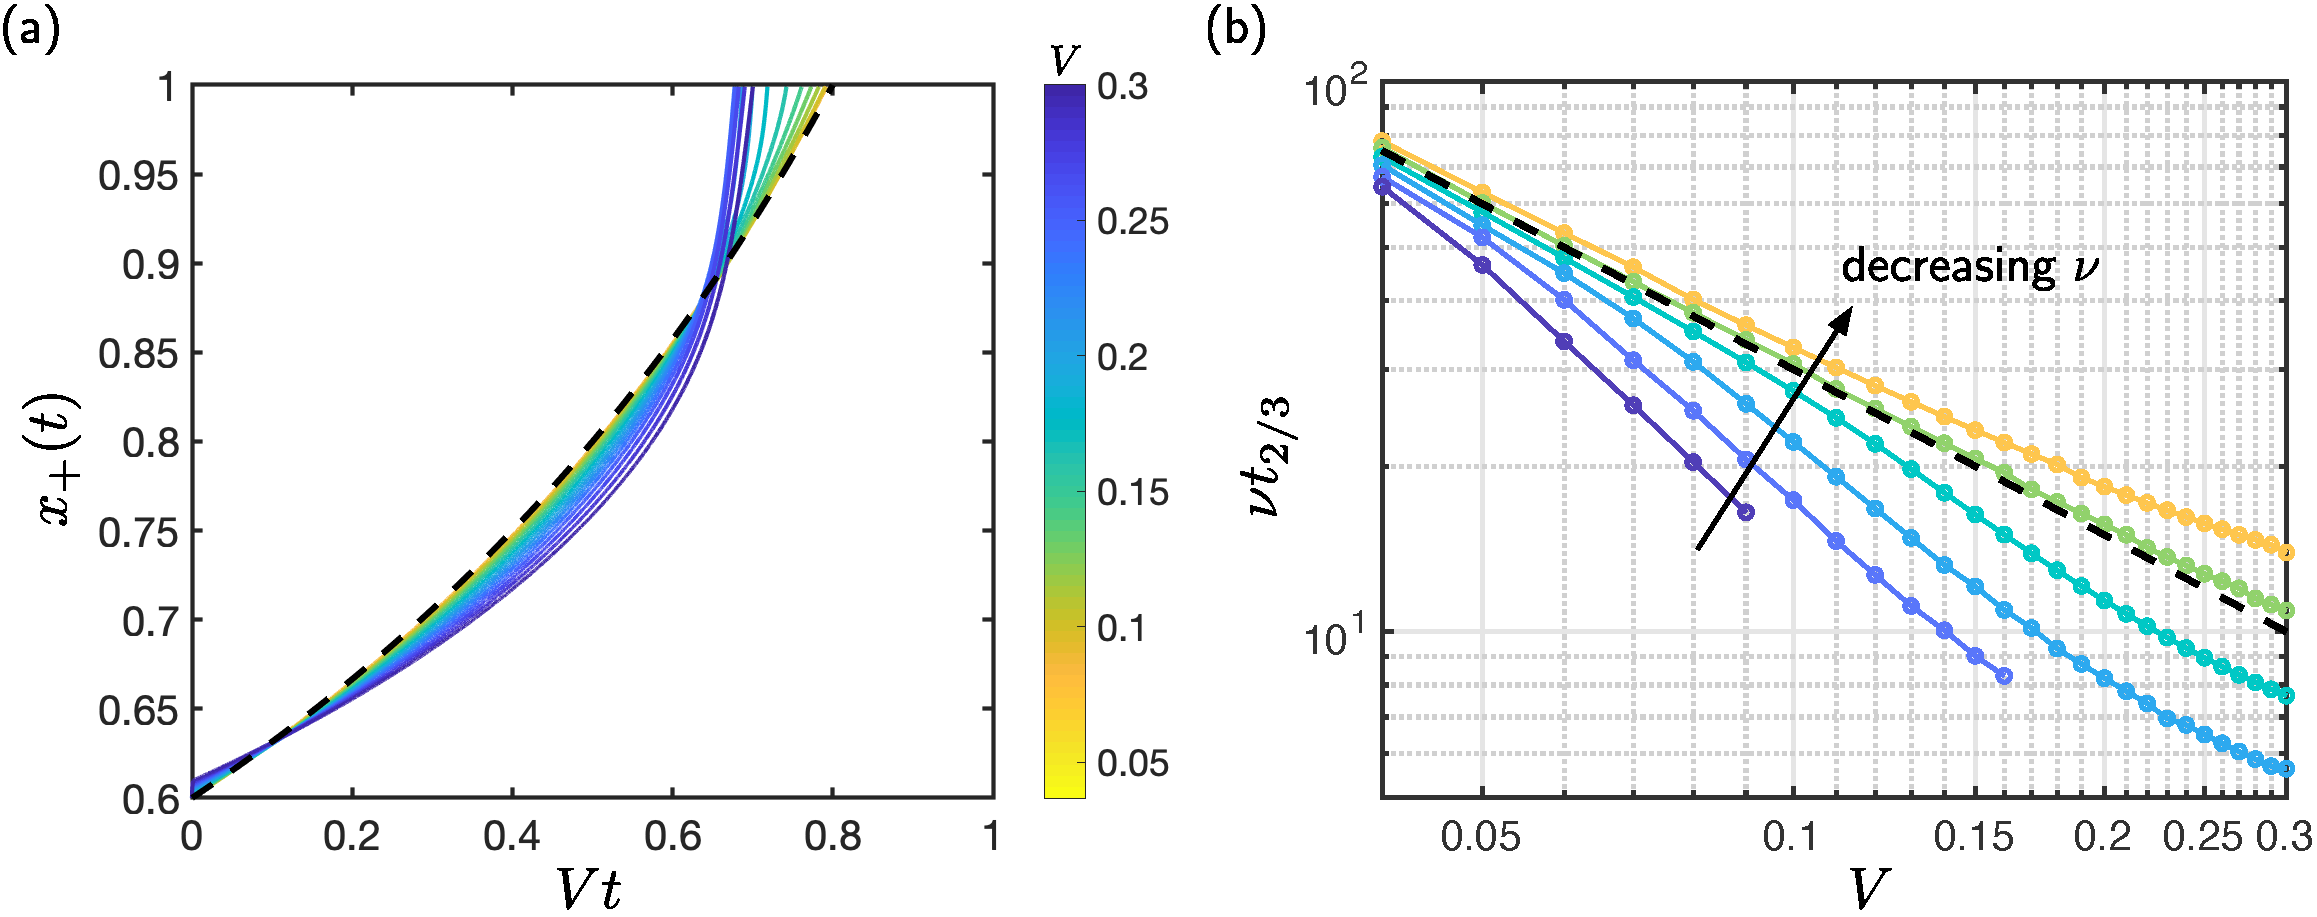
\includegraphics[width = 0.95\textwidth]{SmallDropletsAsymptotics}
\caption{Comparison of numerical solutions and asymptotic results for small droplets. (a) Trajectories $\xright(t)$ (solid curves, with $V$ indicated by the colour bar), obtained by solving the model equations numerically, and the asymptotic result~\eqref{A:E:Ch2:SmallDroplets:SolutionMeniscusPos} (dashed curve). Here, $\xright^0 = 0.6$ and $\nu = 5$. (b) Log-log plot of numerically obtained values of  $\nu t_{2/3}$ (dotted curves) for $\nu = 1,3,5,7,9,11$ and the asymptotic result~\eqref{A:E:Ch2:SmallDroplets:Solutiontf} (dashed line). The curves at larger $\nu$ values terminate when the channel ends touch before the droplet reaches the free end. }\label{A:fig:Ch2:SmallDroplets}
\end{figure}

\subsection{Doubly clamped configurations}

\begin{figure}[t]
\centering
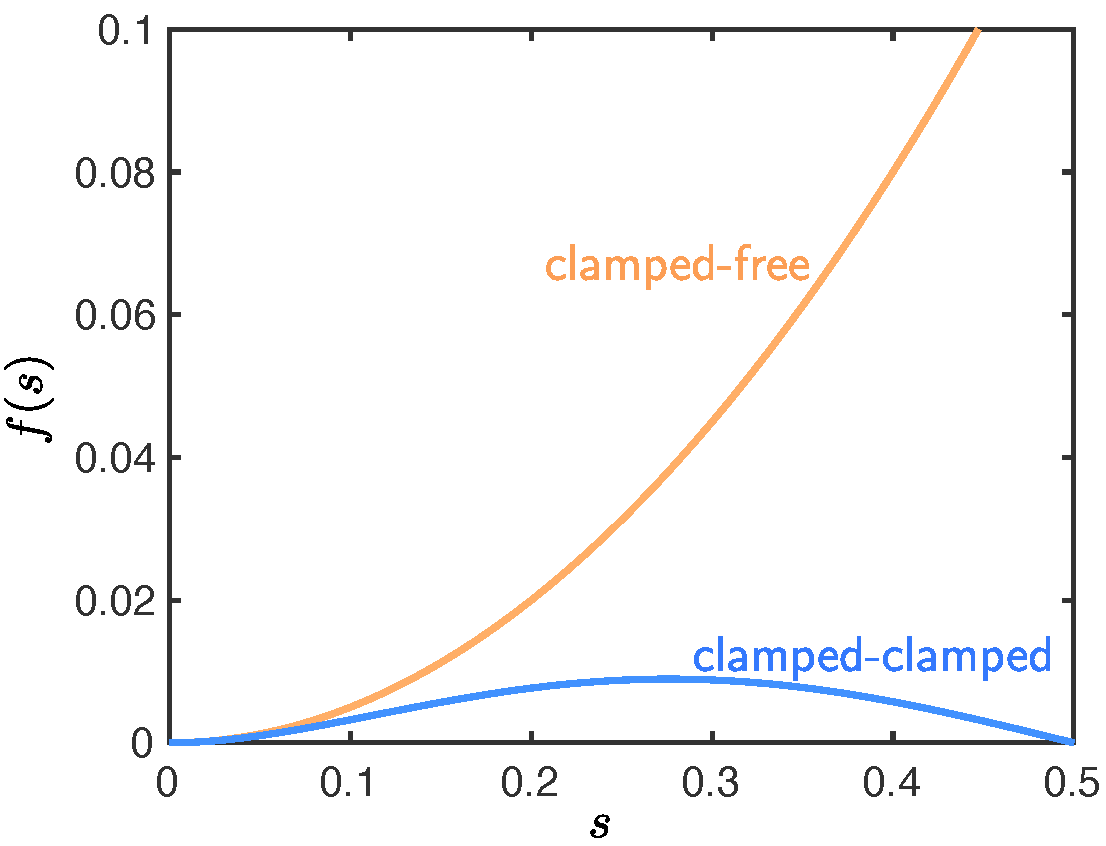
\includegraphics[scale=0.4]{doubly_clamped}
\caption{Plot of the functions $f = f_{\text{clamped}}$ and $f = f_{\text{free}}$ (defined in~\eqref{A:E:Ch2:SmallDroplets:DoublyClamped:xm_ODE_functions}) which describe the speed of small droplets in deformable channels in which both ends are clamped (blue curve) and in channels in which one end is clamped and the other is free (orange curve).}\label{fig:Ch2:Appendix:doubly_clamped}
\end{figure}

In our experimental study of bendotaxis in the following chapter, we encounter the problem of a droplet in a channel that is clamped at both ends. In this section, we consider the behaviour of such a configuration in the case that the droplet is small, $V\ll 1$.

The problem is the same as that in the previous sections of this appendix, but with the free end conditions at $x = 1$ replaced by clamped conditions:
\begin{equation}
h = 0 = \ddp{h}{x} \qquad \text{at}~x = 1.
\end{equation}

We proceed in the same manner as in the clamped-free case of A.1--A.2 by deriving a point force problem. The analysis of Appendix \ref{A:Ch2:SmallDroplets:SmallVolumeExpansion} (in particular, the ODE~\eqref{A:E:Ch2:SmallDroplets:ReducedKinematic}) is still applicable. As we shall see, the jump conditions~\eqref{A:E:Ch2:SmallDroplets:Slope_and_moment_small} are still applicable, but because of the different boundary conditions at $x = 1$, they require a different justification.  Note, however, that to justify the jump conditions on the first and second derivatives (equation~\eqref{A:E:Ch2:SmallDroplets:PtForceJump}) it is sufficient to show that the moment and shear are $\mathcal{O}(V)$.

To make this justification, we first note that the clamped end at $x = 1$ results in effective boundary conditions
\abeqn{A:E:Ch2:SmallDroplets:DoubleClamped:EffBCXright}{
\ddp{^2 h}{x^2} = \frac{2}{\xright^2}\left(2\xright \ddp{h}{x} - 3h + 3\right), \quad \ddp{^3 h}{x^2} = \frac{6}{\xright^3}\left(\xright \ddp{h}{x} - 2h + 2\right)}
at $x = \xright$ (as discussed in \S\ref{S:Ch2:Numerics:Scheme} for the clamped end at $x = 0$).

Let us assume that the channel slope remains small  $\partial h_1 /\partial x = \mathcal{O}(1)$; as we shall see, this is satisfied provided that $\nu = \mathcal{O}(1)$.  Inserting the small deflection ansatz~\eqref{A:E:Ch2:SmallDroplets:Expansion} into~\eqref{A:E:Ch2:SmallDroplets:DoubleClamped:EffBCXright} gives
\begin{equation}
\left.\ddp{^2 h}{x^2}\right|_{x = \xright} =\left. \frac{2}{\xright^2}\left[2\xright V\ddp{h_1}{x} - 3(1 + V h_1) + 3\right]\right|_{x = \xright} + \mathcal{O}(V^2)  =   \mathcal{O}(V)
\end{equation}
and
\begin{equation}
\left.\ddp{^3 h}{x^3}\right|_{x = \xright} =\left. \frac{6}{\xright^2}\left[\xright V\ddp{h_1}{x} - 2(1 + V h_1) + 2\right]\right|_{x = \xright} + \mathcal{O}(V^2)  =   \mathcal{O}(V).
\end{equation}
The moment and shear at $x  = \xright$ are both therefore $\mathcal{O}(V)$ as required, and so the jump conditions across the droplet are identical for both the clamped-clamped and clamped-free configurations.

The leading order point force problem for $h_1$ in the clamped-clamped configuration is therefore
\begin{equation}\label{A:E:Ch2:SmallDroplets:DoublyClamped:PtForcePDE}
\ddp{^4 h_1}{x^4} = 0, \qquad \text{in}~0< x < \xright,~\text{and}~\xright < x < 1,
\end{equation}
with jump conditions
\begin{equation}\label{A:E:Ch2:SmallDroplets:DoublyClamped:PtForceJump}
\left[\ddp{^3 h_1}{x^3}\right]_{\xright^-}^{\xright^+} = -\nu, \qquad \left[\ddp{^2 h_1}{x^2}\right]_{\xright^-}^{\xright^+} =0, \qquad \left[\ddp{ h_1}{x}\right]_{\xright^-}^{\xright^+} =0,\qquad \left[h_1\right]_{\xright^-}^{\xright^+} = 0,
\end{equation}
and boundary conditions
\begin{equation}\label{A:E:Ch2:SmallDroplets:DoublyClamped:PtForceBC}
h_1 = 0 = \ddp{h_1}{x}, \qquad\text{at}~x = 0, 1.
\end{equation}

The solution to~\eqref{A:E:Ch2:SmallDroplets:DoublyClamped:PtForcePDE}--\eqref{A:E:Ch2:SmallDroplets:DoublyClamped:PtForceBC} is
\begin{equation}\label{A:E:Ch2:SmallDroplets:DoublyClamped:SolutionShape}
h_1(x,t) = \begin{cases}{}
       1 + Ax^2 + Bx^3& \text{for }\quad 0 < x < \xright(t), \\
  1 + C(1-x)^2 + D(1-x)^3& \text{for }\quad \xright(t) < x < 1.
        \end{cases}
\end{equation}
where
\begin{align}
A &= -\frac{\nu\xright}{2} \left(\xright^2 + 2\xright -1\right),&  B &= \frac{\nu}{6}\left(2\xright^3 - 3\xright^2 + 1\right),\label{A:E:Ch2:SmallDroplets:DoublyClamped:SolutionShapeCoeffs1}\\
C &= \frac{\nu\xright^2}{2}\left(\xright -1\right), & D&= -\frac{\nu\xright^2}{2}\left(\xright -1\right)\label{A:E:Ch2:SmallDroplets:DoublyClamped:SolutionShapeCoeffs2}
\end{align}
(The solution~\eqref{A:E:Ch2:SmallDroplets:DoublyClamped:SolutionShape} informs us that the channel slope remains small, $\partial h/\partial x \sim \mathcal{O}(V)$, provided that $\nu =  \mathcal{O}(1)$).

Inserting~\eqref{A:E:Ch2:SmallDroplets:DoublyClamped:SolutionShape}--\eqref{A:E:Ch2:SmallDroplets:DoublyClamped:SolutionShapeCoeffs2} into the kinematic condition~\eqref{A:E:Ch2:SmallDroplets:ReducedKinematic} gives the ODE
\begin{equation}\label{A:E:Ch2:SmallDroplets:DoublyClamped:xm_ODE}
\dd{\xright}{t} = \frac{\nu V}{6}\frac{\xright^2(1-2\xright) (\xright -1)^2}{2}.
\end{equation}
Note that~\eqref{A:E:Ch2:SmallDroplets:DoublyClamped:xm_ODE} is anti-symmetric about $\xright = 1/2$, so the system is in equilibrium when the droplet sits at the centre of the channel. Furthermore, the channel deformation is maximised when the droplet sits at the centre, with deformation
\begin{equation}\label{A:E:Ch2:SmallDroplets:DoublyClamped:first_order_deformation}
1 - h(x = 1/2,t) = \frac{V \nu}{192}.
\end{equation}

Figure~\ref{fig:Ch2:Appendix:doubly_clamped} compares the functions
\begin{equation}\label{A:E:Ch2:SmallDroplets:DoublyClamped:xm_ODE_functions}
f_{\text{clamped}}(s) = \frac{s^2(2s-1)(s-1)^2}{2}, \quad \text{and}\quad f_{\text{free}}(s) = \frac{s^2}{2},
\end{equation}
which describe how the speed of the meniscus changes as the droplet moves along the channel (see equations~\eqref{A:E:Ch2:SmallDroplets:xrightODE} and~\eqref{A:E:Ch2:SmallDroplets:DoublyClamped:xm_ODE}). We note that $f_{\text{free}}(s) > f_{\text{clamped}}(s)$ throughout $|s| < 1/2$, and conclude that motion is always quicker when the end $x = 1$ is free, rather than clamped, in the small $V$ case. In particular, for $\xright > 0.37$, the motion in the clamped-clamped case will be at least an order of magnitude slower than that with a free end.

In addition
\begin{equation}\label{A:E:Ch2:SmallDroplets:DoublyClamped:xm_ODE_function_expansion}
f_{\text{clamped}}(s) \sim \frac{1}{16}\left(s - \frac{1}{2}\right) \qquad \text{as}~s \to \frac{1}{2},
\end{equation}
so the droplet approaches the equilibrium at $\xright = 1/2$ like
\begin{equation}\label{A:E:Ch2:SmallDroplets:DoublyClamped:xm_ODE_function_expansion_result}
\xright -\frac{1}{2}\sim \exp \left(-\frac{\nu V t}{48}\right).
\end{equation}
Returning to dimensional units, equation~\eqref{A:E:Ch2:SmallDroplets:DoublyClamped:xm_ODE_function_expansion_result} means that the time scale of relaxation to equilibrium in the doubly clamped channel is
\begin{equation}\label{A:E:Ch2:SmallDroplets:DoublyClamped:xm_ODE_relaxation_timescale}
T =\frac{48}{\nu V t_c}= \frac{48\mu B H}{\gamma^2 \cos^2 \theta_e \Delta X L}.
\end{equation}
We will return to~\eqref{A:E:Ch2:SmallDroplets:DoublyClamped:first_order_deformation} and~\eqref{A:E:Ch2:SmallDroplets:DoublyClamped:xm_ODE_relaxation_timescale} in the following Chapter.

\end{subappendices}
}
%%%%%%%%% Graphics Path %%%%%%%%
%%  Graphics path will need modifying for master compile (i.e. uncomment next line)
\graphicspath{{./Sections/Chapter3_experiments/Figures/}}

%%%%%%%%%%%%%%%%%%%%%%%%
\chapter{Experimental study of bendotaxis}
In this chapter, we describe a series of experiments, similar to the proof of concept experiment presented in Chapter 1. These experiments provide a robust test of our model and offer further insight into the dynamics of bendotaxis. Systematic experiments were performed with both wetting and non-wetting configurations. However, the treatment of the channel walls required to minimize contact angle hysteresis (discussed further below) leads to some uncertainties in the relevant parameters; we therefore focus primarily on experiments with wetting drops but discuss non-wetting configurations in Appendix~\ref{Appendix:Ch3:NonWetting}. %I think we should include non-wetting configurations to be included (a) it's interesting- why does it do this, somebody might want to find out more details... (b) it removes the obvious question of why didn't you do non-wetting experiments. We don't need to claim we're looking for quantitative agreement!

\section{Experimental setup}\label{S:Ch3:ExperimentalSetup}
\begin{figure}
\centering
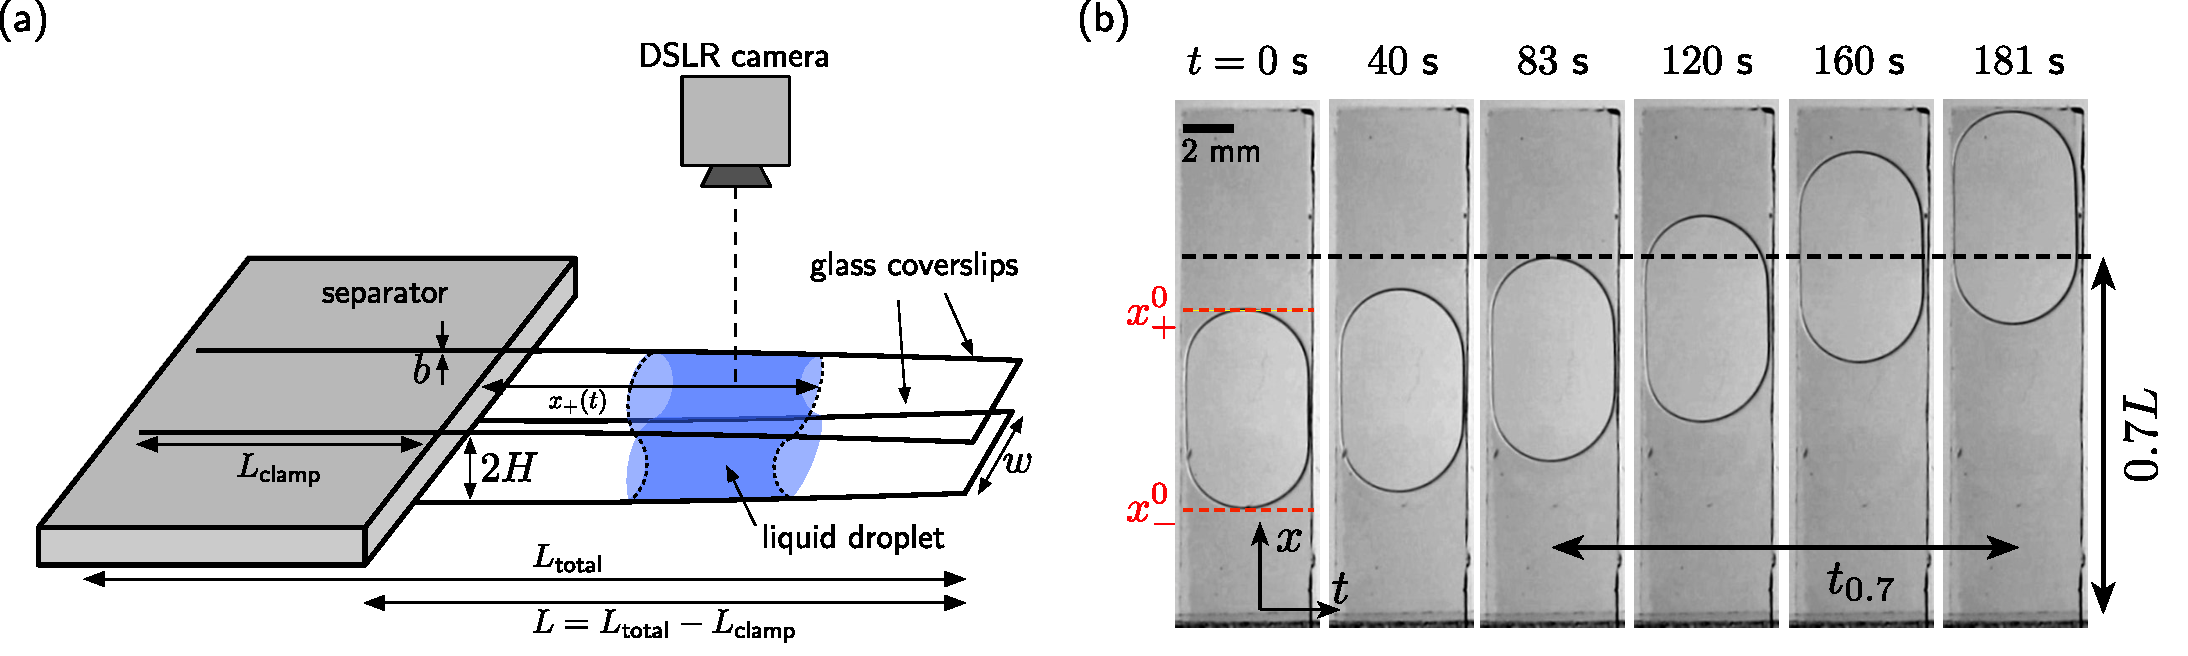
\includegraphics[width = \textwidth]{ExptSetup}
\caption{Experimental study of bendotaxis. (a) Schematic of the experimental setup consisting of a droplet in a flexible channel of undeformed wall separation $2H$, width $w$, and length $L$. We track the leading meniscus, located a distance $\xright(t)$ (measured along the centreline of the channel), during the experiment. (b) Top view of an example experiment with a V50 silicone oil droplet of volume $18~\si{\micro}$L. Here, $2H = 310$~$\si{\micro}$m, $L = 18$~mm, $w = 5$~mm,  and $b = 300$~$\si{\micro}$m. The scale bar indicates $2$~mm. The quantity $t_{0.7}$ is the time taken between $\xright = 0.7L$ and $\xright = L$, which corresponds to the time between the third and sixth images here.}
\label{fig:Ch3:ExptSetup}
\end{figure}
\subsection{Channel fabrication}\label{S:Ch3:ExperimentalSetup:Manufacture}
The experimental setup is shown in Figure~\ref{fig:Ch3:ExptSetup}.  To fabricate the channel, we cut two sections of borosilicate glass cover slips to a width $w$ from larger cover slips of length $L_{\text{total}}$. These coverslip sections were first treated (see below) before being clamped either side of a rigid separator of thickness $2H$ over a length $L_{\text{clamp}}$, to create an open-ended channel of length $L = L_{\text{total}} - L_{\text{clamp}}$ and half-thickness $H$.

%Why do we need to control tapering and how did we control it
Since the liquid motion is driven by a droplet induced tapering, we were careful to ensure that the channel has as little intrinsic tapering as possible. Intrinsic tapering is known to drive droplet motion, as studied by~\cite{Renvoise2009EPL} and~\cite{Reyssat2014JFM}, and including it here would interfere with the self-induced droplet motion of interest. To minimise intrinsic tapering, we clamped the channel walls over a length at least as long as the length of the resulting channel, i.e.~$L \lesssim L_{\text{clamp}}$ (Figure~\ref{fig:Ch3:ExptSetup}(a)).

\subsection{Channel wall treatment}\label{S:Ch3:ExperimentalSetup:WallTreatment}
The coverslips that make the channel walls were treated to minimize dissipation arising from dynamic contact angle effects and contact line pinning. As we shall see in the following chapter, the dynamics of bendotaxis is highly sensitive to contact angle hysteresis, which we have not yet included in our model. (In addition, recent studies of droplet dynamics in tapered channels by~\cite{Prakash2008Science} and~\cite{Bush2010AdvCollIntsci} have demonstrated how droplet motion can be arrested completely by contact angle hysteresis.)

We used two different treatments on the coverslips, which are described briefly here (full details can be found in Appendix~\ref{Appendix:Ch3:SurfaceCoating}). In one set of experiments, the glass was treated (prior to the channel fabrication) to render it a slippery lubricant-infused porous surface (SLIPS). Briefly, this treatment involves introducing a porous matrix to the surface of the coverslips, into which a lubricating silicone oil is impregnated. The result is an intrinsically smooth surface with no contact line pinning, since droplets of silicone oil subsequently introduced onto it share an interface only with the lubricant~\citep{Wong2011Nature}.

In the second set of experiments, the channel walls were pre-wetted with the same liquid as was used for the subsequent experiments in that channel. This treatment took place after the channel had been assembled. We ensured that the prewetting layer was sufficiently thin that liquid entrained during the experiment did not significantly alter the droplet's volume (Appendix~\ref{Appendix:Ch3:SurfaceCoating}).

%why use SLIPS vs why use prewetting. SLIPS: no hysteresis but do introduce dissipation in underlying film. Prewetting - ease.
The advantage of using SLIPS treated, rather than pre-wetted, coverslips for the channel walls is that this treatment guarantees low contact angle hysteresis and contact line dissipation.  The SLIPS treatment is, however, relatively resource intensive (by comparison with the pre-wetting treatment) and introduces another source of dissipation not accounted for by our model, namely viscous dissipation in the lubricant layer~\citep{Keiser2017SoftMatter}.

We find no difference between the SLIPS and pre-wetting treaments in our experimental data (Appendix~\ref{Appendix:Ch3:SurfaceCoating}). We interpret this agreement as evidence that contact line dissipation is negligible in the pre-wetting case, and lubricant dissipation is negligible in the SLIPS case. Henceforth, we shall not distinguish between the two cases.

\subsection{Experimental protocol}\label{S:Ch3:ExperimentalSetup:Performing}
Before the experiment began, a light spacer of thickness $2H$ was introduced to separate the free ends of the channel -- this allowed us to control the time at which the experiment begins. A liquid droplet of volume $\Omega$ was introduced close to the centre of this `doubly-clamped' channel using a micropipette with a narrow syringe tip (diameter 250~$\si{\micro}$m) attached. After deposition, the droplet sits at (what will become) its initial position.

Note that the clamped-clamped channel did experience a deformation in response to the presence of a droplet being introduced, but this deformation was relatively small. To justify this, we consider the limit of small droplets (which, as we shall see, predicts the dynamic behaviour of finite size droplets reasonably well). As demonstrated in Appendix A.3 of Chapter 2, a clamped-clamped channel does experience a deformation when a droplet is introduced but it is relatively small -- the maximum deformation is
\begin{equation}
\frac{\nu V H}{192} = \frac{\gamma \cos \theta_e L^3  \Delta X}{192 B H^2} H
\end{equation}
We have $\gamma \cos \theta_e L^3 \Delta X/(192 B H^2) < 0.02$ in all of our experiments: the channel deformation in the clamped-clamped state is never more than (approximately) 2\% of the channel half-width.

More important is the time scale of motion of a droplet in the clamped-clamped channel: in Appendix A.3 of Chapter 2, we also showed that, for a small droplet close to the centre of the channel, this time scale of droplet motion is
\begin{equation}
T = \frac{48 \mu B H}{\gamma^2 \cos^2 \theta_e \Delta X L},
\end{equation}
which is significantly longer ($\mathcal{O}$(10~minutes)) than the time spent in the clamped-clamped state ($\mathcal{O}$(10~seconds)). It is therefore reasonable to neglect any motion in the doubly clamped state, and, in particular, to assume that the droplet's position when it is deposited in the clamped-clamped configuration is the initial condition in the subsequent experiment.

The droplet was photographed in the clamped-clamped configuration using a DSLR camera (Nikon D700) mounted above the experiment. This image (and images of the subsequent experiment) have a resolution $1920\times1080$ pixels, with a typical spatial resolution of $0.03$~mm per pixel. Using this image, we determined $x_{\pm}(t = 0)$, the initial positions of the menisci -- measured along the centreline of the channel -- and thus the droplet length $\Delta X = \xright(t = 0) - \xleft(t = 0)$ and the relative volume $V = \Delta X /L$. To improve the contrast of the menisci, which appear as dark outlines, in images taken from above (Figure~\ref{fig:Ch3:ExptSetup}(b)), we lit the experiment from below (the curved interfaces at the menisci refract the light).

Droplets were heterogeneous in the third spatial direction (the direction that is not included in the model of Chapter 2, see Figure~\ref{fig:Ch3:ExptSetup}(b)) and the meniscus positions are measured at the droplet's longest point, so $V$ is an overestimate of the relative volume: $V = \Delta X/L > \Omega/(2H Lw)$. (The latter measure of relative volume was not used because there is large uncertainty in the actual amount of liquid that enters the channel.) Another important consequence of this heterogeneity is the presence of an interfacial curvature in the third spatial dimension (Figure~\ref{fig:Ch3:ExptSetup}(b)). However, this curvature, $\kappa_2 \sim L/w^2$, was relatively small in comparison with the curvature $\kappa_1 \sim 1/H$ of interest, for all parameter values considered.

When the spacer was removed, the droplet moved spontaneously towards the free end of the channel. The experiment was lit brightly from below and photographed from above with the same camera as described for determining the initial condition. The camera recorded one image every second. When the droplets reached the free end, we typically observed a small retreat of the rear `$-$' meniscus, after which the droplet remains stationary; the experiment concluded after the droplet had sat stationary (measured by eye) for $30$~s. Afterwards, the channel was disassembled and the wall thickness $b$ and spacer thickness $2H$ were measured with digital callipers (as a result, each experiment required a new channel to be fabricated).

As mentioned, the menisci are clearly visible as dark outlines in the images taken during the experiment (Figure~\ref{fig:Ch3:ExptSetup}(b)). A Canny edge detection algorithm~\citep{Canny1987} incorporated into a custom image analysis code written in
\textsc{matlab} was used to determine the outline of the droplet in the images taken during the experiment. Using the length of the channel to determine the spatial resolution of the images, we inferred from these outlines the meniscus trajectory $\xright(t)$ in each experiment.

Finally, to determine the effects of evaporation, several experiments were left in their `final' configuration overnight. No observable change in size or position had occurred by the next morning. This is consistent with our modelling assumption that evaporation is negligible.

\subsection{Parameter study}\label{S:Ch3:ExperimentalSetup:ParameterStudy}
%Describe ensemble
We performed the bendotaxis experiment 142 times in total. The liquid viscosity $\mu$, channel length $L$, channel thickness $2H$, droplet volume $\Omega$, and coverslip thickness $b$ were systematically varied across these experiments. The channel width $w = 5\pm0.5~\si{m\meter}$ and liquid--vapour interfacial tension $\gamma $ (see below) were held constant across the experiments. This channel width $w$ was the smallest we can reliably achieve -- cover slips typically fractured when cut to widths narrower than this (it is desirable to minimise the channel width $w$ as this reduces the influence of flow and cross-sectional volume variations in the spatial direction not accounted for by our model).

%Go through variation in each parameter: liquid viscosity
For each experiment, we used silicone oil (Sigma-Aldrich, USA) as the droplet liquid. We used silicone oils V50, V100, V350, and V500 with dynamic viscosities $\mu  = 48, 96, 336, 480~\si{\pascal~\second} \pm 5\%$ respectively (note that we calculate the dynamic viscosity as the product of the kinematic viscosity and density, whose values are provided by the manufacturer). These liquids have the same surface tension coefficient, $\gamma = 22 \pm 1~\si{m\newton}~\si{\meter}^{-1}$ (also provided by the manufacturer). Owing to the channel wall treatment, the silicone oil droplets share an interface only with the (lubricating) silicone oil and thus perfectly wet the channel walls ($\theta_e \approx 0$), but crucially form a capillary bridge with well-defined menisci.

Droplet volumes $\Omega$ in the range $10 \leq \Omega \leq 25 \pm 0.5~\si{\micro}\si{\liter}$ were used.

Each of the coverslips (Agar Scientific, UK) has a fixed length $L_{\text{total}} = 64~\si{\milli\meter}$; the channel length is varied in the range $14 \leq L \leq 30 \pm 0.25~\si{\milli\meter}$ by adjusting the clamped length, $L_{\text{clamp}}$. Whilst it would be desirable to probe a larger range of channel lengths (recall that our theory predicts sensitive dependence on $L$ through the bendability $\nu \sim L^4$), the upper bound on the channel length was chosen so that all configurations have a  pressure gradient contribution from gravity (defined in \S2.1) that is less than 10\% of the total pressure gradient. In addition, longer channels are more likely to have walls touch during the motion (at which point our theory breaks down). Finally, for channels with $L < 14~\si{\milli \meter}$, we observe that droplets do not occupy a significant portion of the channel and are pancake shaped; for these droplets, a two-dimensional theory is inadequate.

The separator, which sets the thickness of the channel, is fabricated by adhering two or more glass coverslips together. Using this method we achieved channel thicknesses  $310 \leq 2 H_0 \leq 630 \pm 5~\si{\micro}\si{\meter}$. (Note that each spacer is measured individually using a digital micrometer as the thickness of the adhesive layer used in fabricating the spacer is not known a priori).

We used three different thicknesses of coverslip (labelled no.~$1,1.5,$ and $2$ by the manufacturer) giving channel wall thicknesses in the range $160 \leq b \leq 310 \pm 5~\si{\micro}\si{\meter}$. (Note that if there is a difference in the measured values of $b$ between the upper and lower wall, we take the mean of the two values.)

With these parameter values, we achieve a large variation in the elasto-capillary number, $0.16 \leq \nu \leq 8$, as well as relative volumes in the range $0.20 \leq V \leq 0.51$. The combination of these results in almost two orders of magnitude variation in $\nu V$,  $0.24 \leq \nu V \leq 20$.

\section{Results}
\begin{figure}[h!]
\centering
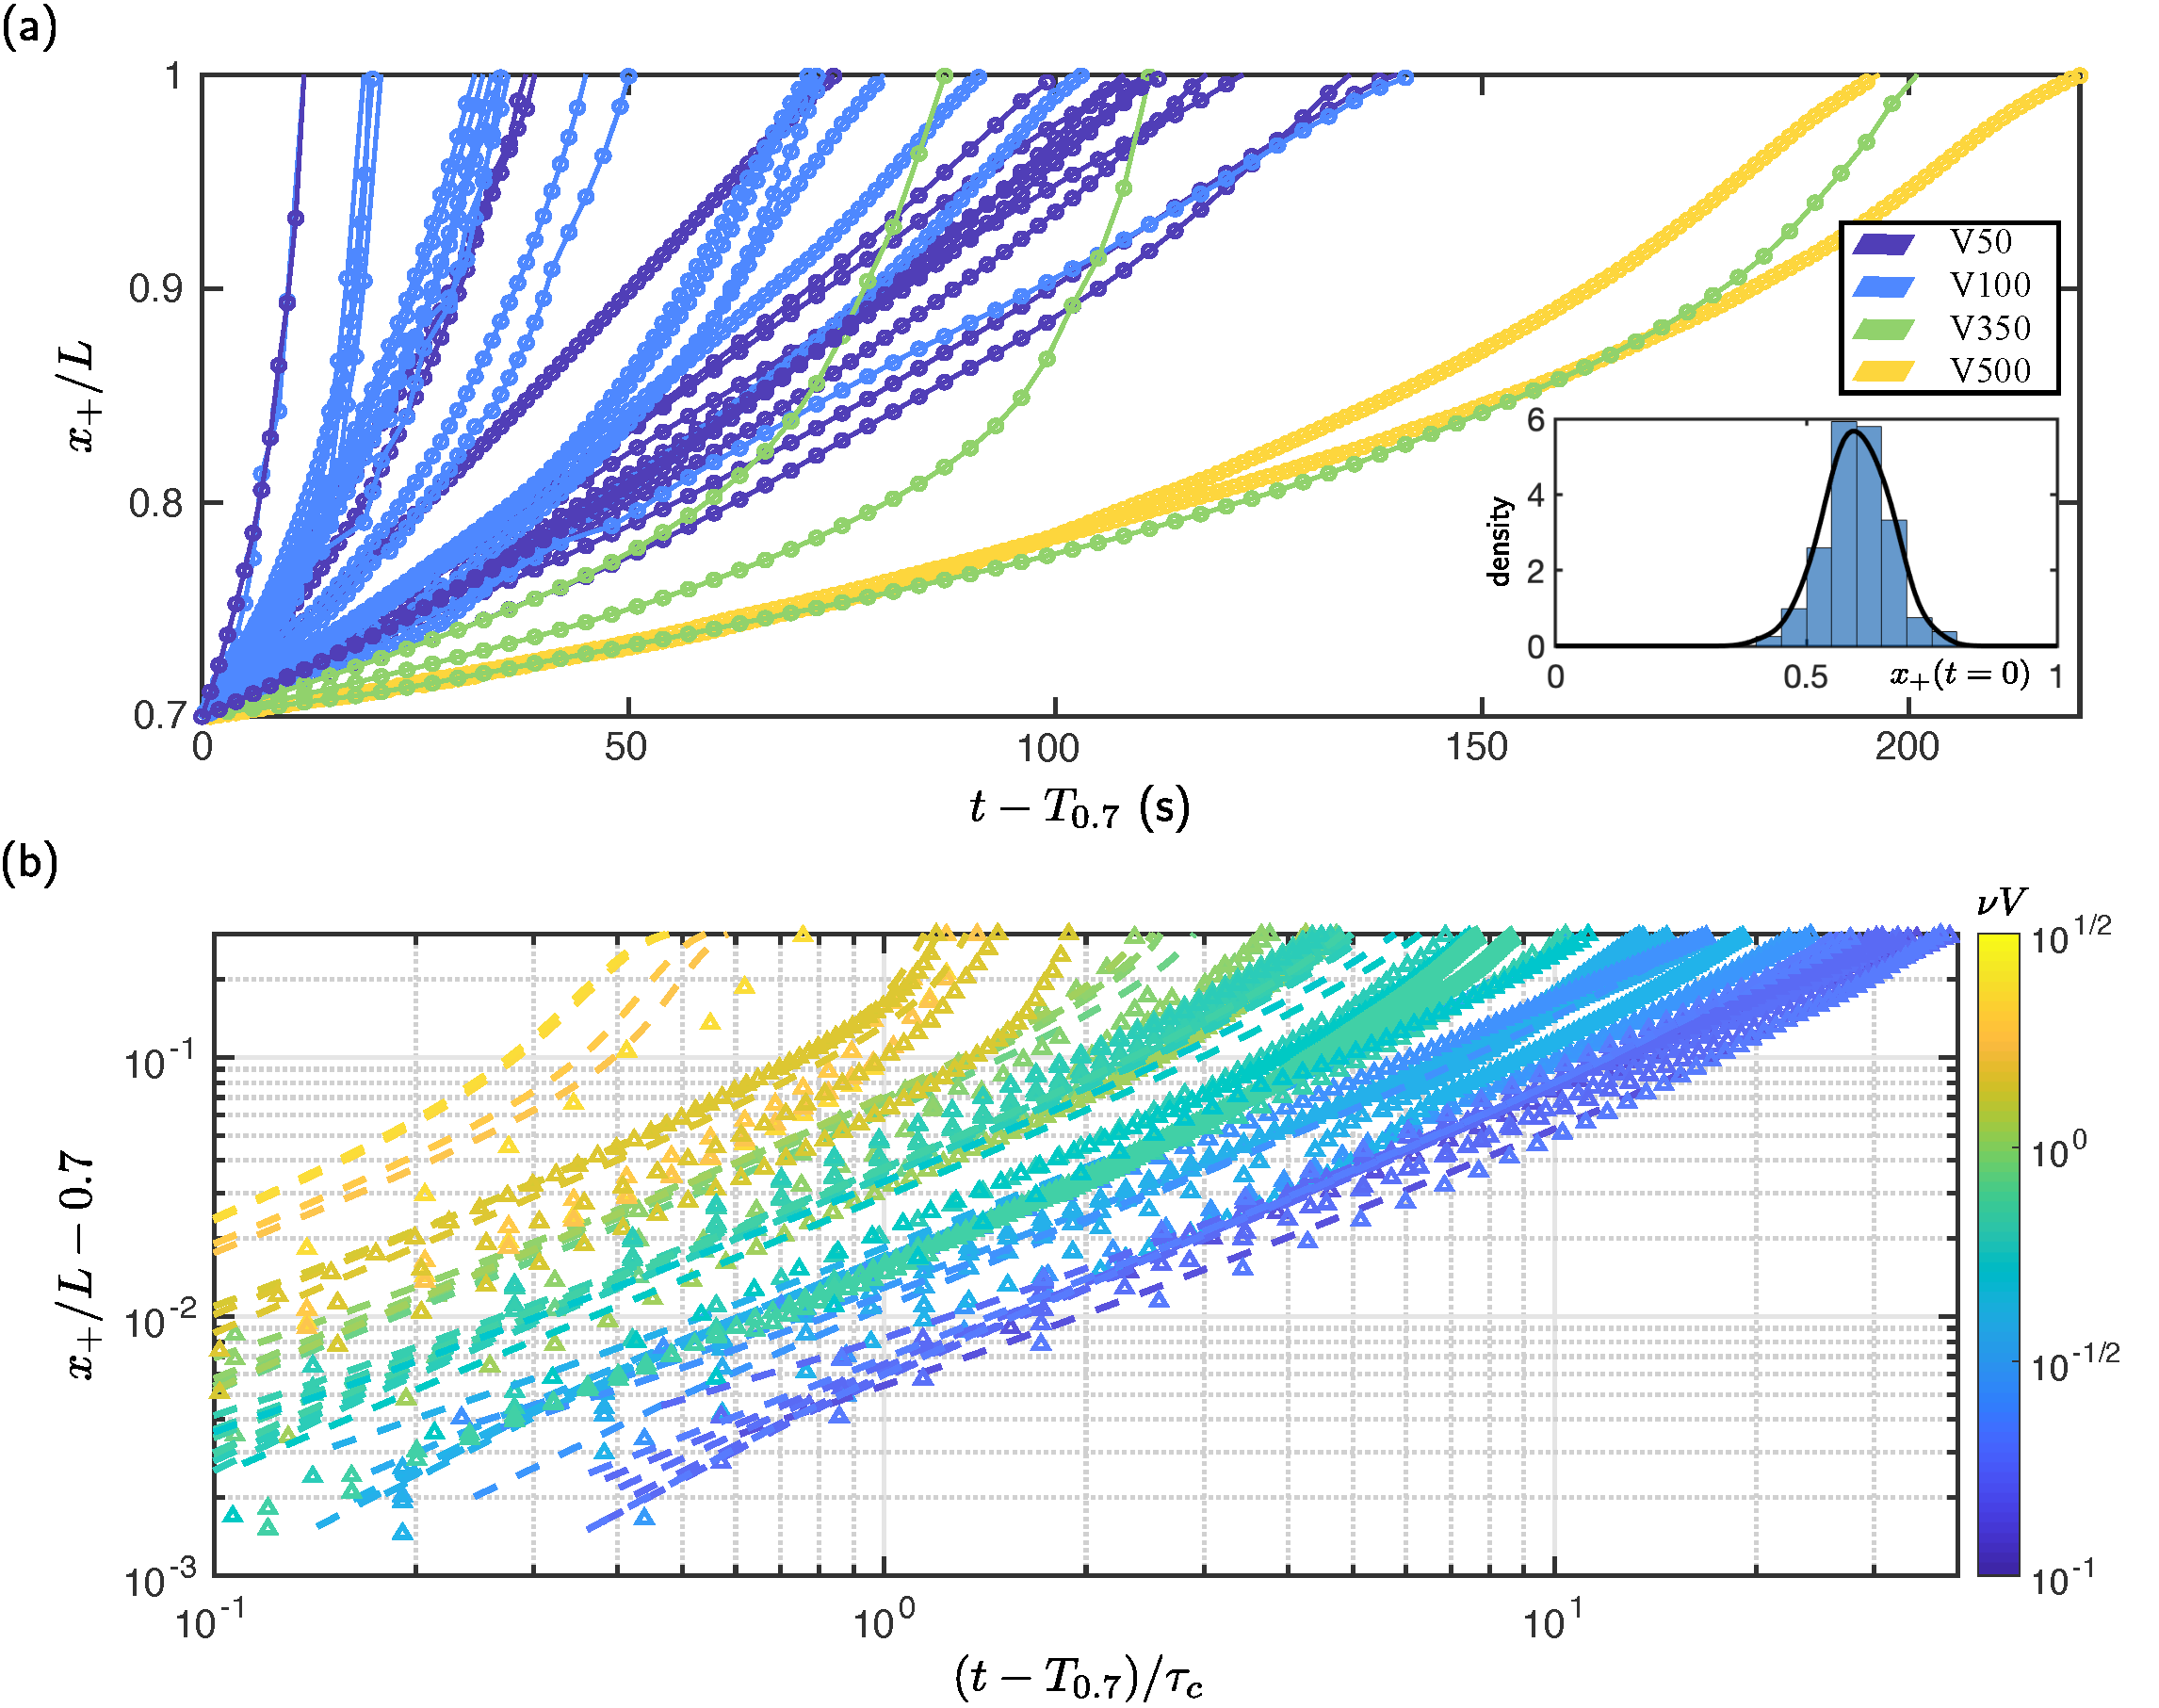
\includegraphics[scale=0.39]{ExptsFigV3}
\caption{(a) Trajectories of the meniscus displacement away from $t = T_{0.7}$, at which point $\xright = 0.7L$. Each curve corresponds to an individual experiment (which has a unique value of $T_{0.7}$). Circles indicate experimental data, obtained at 1~s intervals, connected by a spline to facilitate distinction between individual experiments. The legend indicates the type of silicone oil (and hence droplet viscosity) used in each experiment. Inset: histogram (blue boxes) and kernel density estimate (black line) of the initial conditions $\xright(t=0)/L$ in all 142 experiments. (These plots are scaled so that their total area is unity.) (b) Plot of the (displacement) trajectories shown in (a) as a function of dimensionless time on logarithmic axes (to facilitate identification of distinct trajectories). Triangles indicate experimental data and dashed curves indicate numerical solutions of the model equations (presented in \S2.2) using parameter values corresponding to the experiment. Points (both experimental and numerics) are coloured according to the value of $\nu V = BH^2 / (|\gamma \cos \theta_e|\Delta X L^3)$.}\label{fig:Ch3:ExptRawAndScaledTraces}
\end{figure}


\subsection{Raw results}
After image processing, each experiment yields a meniscus trajectory $\xright(t)$ with initial condition $\xright(0)$. Standardizing of initial conditions is difficult (it relies on the accuracy of inserting the droplet by hand), so we end up with a broad range of initial droplet positions $0.42 <\xright(t = 0)/L < 0.76$ with mean 0.6 and standard deviation 0.06 (the inset in Figure~\ref{fig:Ch3:ExptRawAndScaledTraces}(a) contains a plot of the kernel density estimate~\citep{Sheather2004StatSci} of $\xright/L$).

We do not directly compare experimental trajectories, as their behaviour is obfuscated by this difference in initial condition. Instead, we consider shifted trajectories:  we choose a point $0 < p < 1$ and determine the time, $T_p$, at which this trajectory passes $p$. We then define the shifted time $\tilde{t} = t - T_p$. We also consider the dimensionless displacement $\xright/L - p$, rather than the raw meniscus position. (Note that $T_p$ is related to the dimensional form of the quantity $t_f$ -- the time between the events $\xright/L = f$ and $\xright = 1$ --  by $T_f + t_f = t_{\text{total}}$, where $t_{\text{total}}$ is the time taken for the droplet to pass from its initial position to the end at $x = L$.)

Figure~\ref{fig:Ch3:ExptRawAndScaledTraces}(a) contains a plot of the trajectories $\xright(t)/L -  0.7$ (i.e.~taking $p = 0.7$ in the above definition). The data shown in this figure are only for those experiments with initial droplet positions $0.6L < \xright(t = 0) <0.65L$; this restriction ensures that only a manageable set of data (38 out of 142 total experiments) is presented. (Note that this restriction is somewhat arbitrary -- we could equally have taken $0.5L < \xright(t = 0) <0.55L$, for example -- but the particular choice we have made does cover the extremes of the parameter space described in the previous section.)

The trajectories demonstrate the large variation in dynamic behaviour which can be achieved by varying the experimental parameters. For example, the slowest moving droplet takes an order of magnitude longer to move from $\xright/L = 0.7$ to $\xright/L = 1$ (approximately $220$~s for the slowest moving droplet versus approximately $12$~s for the fastest). As expected, the viscosity plays a key role: the trajectories corresponding to high viscosity droplets (yellow and green trajectories in Figure~\ref{fig:Ch3:ExptRawAndScaledTraces}(a)) generally take much longer to traverse the final 30\% of the channel than the relatively low viscosity droplets (blue trajectories in Figure~\ref{fig:Ch3:ExptRawAndScaledTraces}(a)). The trajectories also indicate that droplets accelerate as they move along the channel, as the model developed in previous chapter predicts.

For a more detailed comparison between the model and experimental trajectories, we plot in Figure~\ref{fig:Ch3:ExptRawAndScaledTraces}(b) the trajectories as a function of dimensionless time (non-dimensionalized with the capillary time scale $\tau_c = \mu L^2 / (|\gamma \cos \theta_e| H)$). By plotting in this way, we are able to identify a strong dependence of the dynamic behaviour on the quantity $\nu V = BH^2 / (|\gamma \cos \theta_e|\Delta X L^3)$, which was identified as being important in the scaling argument in \S2.1. Those experiments corresponding to low $\nu V$ take a long time, relative to the capillary time scale (and vice versa for high $\nu V$). We postpone any detailed assessment of experimental dependence on $\nu V$ until the following subsection. 

Alongside each experimental trajectory, we plot in  the prediction of the full model for the appropriate parameter values, obtained using the numerical scheme described in \S2.2 (Figure~\ref{fig:Ch3:ExptRawAndScaledTraces}(b)). In each case, we use the initial conditions from the corresponding experiment. We see reasonable agreement between the numerical solutions and the experimental trajectories, and also that the spread of data -- the difference in time taken between the (relatively) fastest and slowest droplets --  is consistent between experiment and numerics, as is the shape of the trajectories.

Note that the numerical solutions typically overestimate the speed at which the droplets move along the channel (this is most pronounced in the case of large $\nu V$,  the yellow trajectories in Figure~\ref{fig:Ch3:ExptRawAndScaledTraces}(b)); these deviations are in the direction we expect -- neglecting the curvature $\kappa_2$, overestimating the droplet volume and ignoring contact line dissipation, would  each act to slow the droplet down.

%some segue to introducing the dynamic proxy?

\subsection{A proxy for the dynamics}
\begin{figure}[h]
\centering
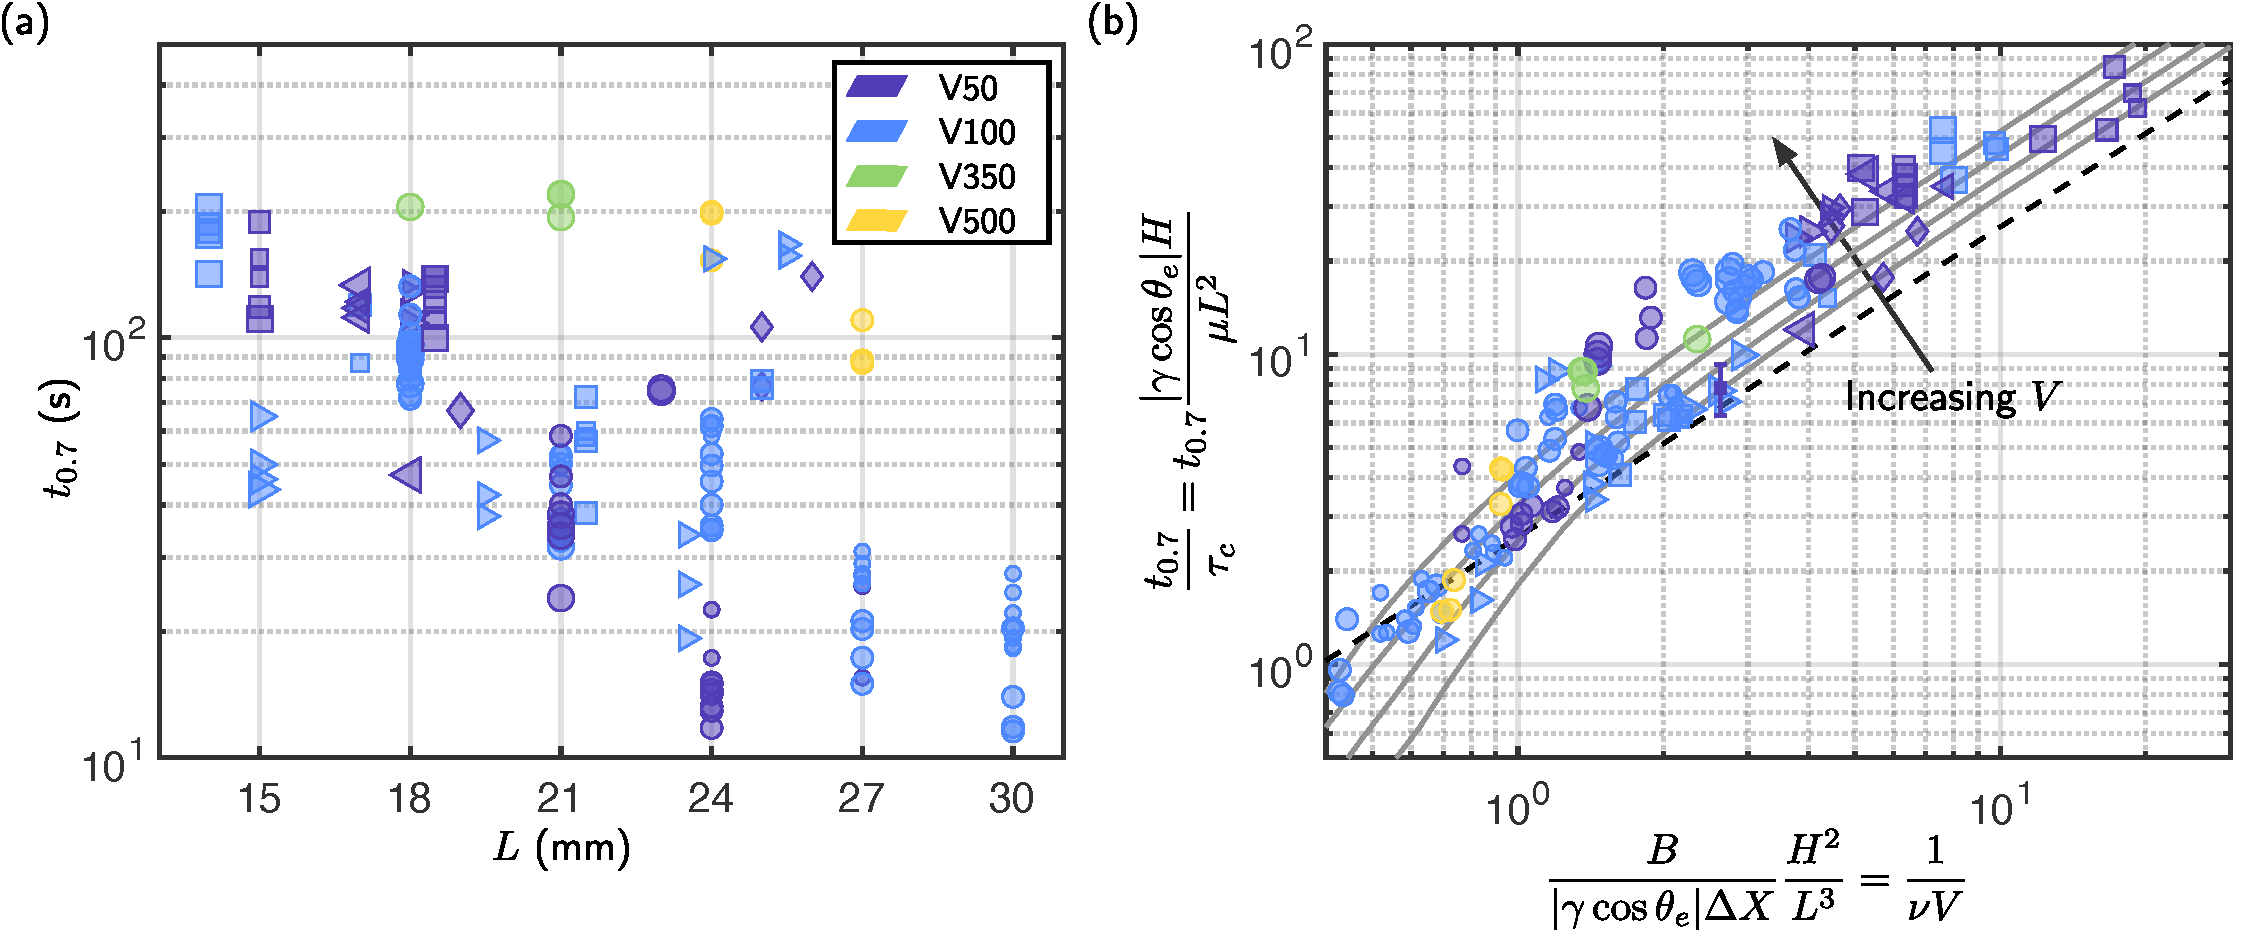
\includegraphics[width = \textwidth]{tpt7_both}
\caption{(a) Raw experimental measurements of $t_{0.7}$ for different channel lengths. The legend indicates the silicone oil used (and hence the viscosity, see main text). Different shapes encode channel wall separation as follows: $2H = 310~ \si{\micro \meter}$ (right triangle), $360 \si{\micro \meter}$ (left triangle), $430 \si{\micro \meter}$ (square),$ 540 \si{\micro \meter}$ (circle),$ 630 \si{\micro \meter}$ (diamond). The size of each point encodes the approximate fraction of the channel taken by the droplet ($V = \Delta X /L$), with bins corresponding to $V = 0.25, 0.25 \leq V < 0.35, 0.35 \leq V < 0.45$, and $V \geq 0.45$. (b) Collapse of the experimental data when rescaled according to~\eqref{E:Ch3:ScalingFunctionalForm_asymptotic}. A single set of error base extends one standard deviation away from a particular data point, computed from 20 measurements (see Appendix~\ref{Appendix:Ch3:SurfaceTreatment:Comparison}). Solid curves shown results from numerical solutions of the equations governing the model. Also plotted as a dashed line is the asymptotic result~\eqref{E:Ch3:ScalingFunctionalForm_asymptotic}, valid for $V \ll 1$ (corresponding to the upper right corner of this plot).}\label{fig:Ch3:RawT23}
\end{figure}

We have seen that the shape of the trajectories is well predicted by the theory. To allow a more robust comparison between the mathematical model developed in the previous chapter and the myriad experimental data (the data plotted in Figure~\ref{fig:Ch3:ExptRawAndScaledTraces} covers approximately 25\% of the the total), we re-introduce $t_f$, the time taken for the droplet to move between $\xright/L = f$ and $\xright / L = 1$. This quantity is a useful proxy to describe the dynamic behaviour throughout the experiment.

%very explicitly: why is t_f better than the full trace
There are two main benefits to considering the quantity $t_f$, rather than the full trajectories. Firstly, we have a single value of $t_f$ per experiment, vastly reducing the amount of data to be presented. Secondly, $t_f$ is approximately independent of the initial conditions and, as a result, removes the need to shift the time origin (this is in contrast to other proxies for the dynamic, such as mean square error between the numerical solution and experimental trajectory). Note, however, that by abstracting in this way, we remove any detail of \textit{how} the droplet gets from $\xright / L = f$ to $\xright / L = 1$ (other than how long it takes).

%what does t_f look like with respect to the model
Recall that the model developed in the previous chapter has three independent parameters: the dimensionless initial droplet position, $x_+(t = 0)/L$, the relative volume $V = \Delta X/ L$, and the bendability $\nu = \gamma \cos \theta_e L^4/(B H^2)$. In our model, however, $t_f/\tau_c$ is approximately independent of initial conditions; the model prediction of $t_f/\tau_c$ depends only on $\nu, V$,
\begin{equation}\label{E:Ch3:ScalingFunctionalForm}
\frac{t_{f}}{\tau_c} = F(\nu, V).
\end{equation}
In particular, the scaling argument in \S2.1 gives this functional dependence as
\begin{equation}\label{E:Ch3:ScalingFunctionalForm_scaling}
\frac{t_{f}}{\tau_c} \sim \frac{1}{\nu V}
\end{equation}
for $V \ll 1$ and $\nu \lesssim 1$. The asymptotic analysis for small droplets (see Appendix A of Chapter 2) gives the pre-factor
\begin{equation}\label{E:Ch3:ScalingFunctionalForm_asymptotic}
\frac{t_{f}}{\tau_c}  = \frac{6(1-f)}{f} \frac{1}{\nu V} \quad \text{as}~ V \to 0.
\end{equation}

%with the proxy, we can show all data and identify strong dependence on geometry which is hidden in the traces
In Figure~\ref{fig:Ch3:RawT23}(a) we present raw measurements of $t_{0.7}$ as a function of the channel length $L$. (Again, taking $f = 0.7$ is arbitrary but this value is sufficiently far from unity to allow a significant portion of the motion to be considered sufficiently. Experiments with $\xright(t =0) > 0.7L$ are then discounted of course, but less than 10\% of the experiments fall into this category.) Plotting the data against the channel length $L$ reveals a strong dependence of the dynamic behaviour on the channel length, which was not visible before. For example, droplets in channel with length $L = 30$~mm take an order of magnitude less time to traverse the final 30\% than droplets of the same viscosity in channels of length $L = 18$~mm.

Rescaling the data according to~\eqref{E:Ch3:ScalingFunctionalForm_scaling} provides a reasonable collapse (Figure~\ref{fig:Ch3:RawT23}(b)). For moderate to large values of the abscissa in Figure~\ref{fig:Ch3:RawT23}, we observe the scaling~\eqref{E:Ch3:ScalingFunctionalForm_scaling}. However, at smaller values of the abscissa (larger $V$), the linear scaling appears to break down.

We also include in Figure~\ref{fig:Ch3:RawT23}(b) curves corresponding to numerical solutions of the model equations for $V = 0.2, 0.3, 0.4, 0.5$ (i.e.~spanning the experimental range). The curves are obtained by numerically solving the model equations repeatedly at fixed $V$; by varying $\nu$ the curves in Figure~\ref{fig:Ch3:RawT23}(b) are traced out. These numerical solutions indicate that the non-linearity observed in the experimental data at small values of $\nu V$ is a real feature of the model that is not captured by the simple scaling argument described in \S2.1. For these experiments, the assumption of small deformations is no longer valid, and droplets traverse the channel quicker than the scaling argument predicts. Physically, this corresponds to the non-linearity in the pressure difference -- which arises when channel deformations are significant -- overcoming the non-linearity in the channel permeability (the former will reduce $t_f$ relative to the small deformation case, while the latter will increase it).

We also note that the spread between the numerical results corresponding to the largest and smallest values of $V$ is comparable to that in the experiments,  suggesting that some of the discrepancy between experiments and the asymptotic prediction~\eqref{E:Ch3:ScalingFunctionalForm_asymptotic} is accounted for by the finite value of $V$.

\section{Summary}
In this chapter we have presented an experimental investigation of bendotaxis. Although the `bench top' experiments are relatively simple, they provide a robust test of the model developed in the previous chapter.

In these experiments, we focussed primarily on the case of wetting droplets and were careful to minimize contact angle hysteresis and contact line dissipation; in the following chapter we consider the effect of contact angle hysteresis on the dynamics of bendotaxis.

The numerically and experimentally obtained droplet trajectories have a similar shape, but the model systematically over-predicts the speed with which droplets will traverse the channel. This is consistent with the two dimensional nature of our model: both interfacial curvature and volume variations in the third spatial dimension -- which are not included in the model -- are expected to slow the droplet down.

We considered the time to traverse a portion of the channel as a proxy for the dynamic behaviour; introducing this proxy facilitated quantitative comparison of a large set of data and reduced sensitivity of the results to initial conditions, which are hard to standardise in experiments. The experimental data for the traversal time indicate that the small deflection result derived in \S2.3 describes the dynamics reasonably well, even when the droplet has finite volume. The deviations from the small droplet result -- the non-linearity associated with large channel deflections, and the finite drop size effects predicted by the model -- are represented in the experimental data.

%couple of paragraphs saying what we did and the main conclusions (it feels like quite a sudden end if not!)

%\begin{appendix}
\begin{subappendices}
\renewcommand{\thesection}{\Alph{section}}
\section{Surface treatments}\label{Appendix:Ch3:SurfaceCoating}
Before each experiment, the glass coverslips were first treated to reduce the amount of contact line pinning and contact angle hysteresis. In this appendix we describe in more detail the two  techniques used to treat the channel walls -- SLIPS treatment and pre-wetting -- as well as additional experiments to test whether there is any difference between the dynamic behaviour in SLIPS treated and pre-wetted  channels.

\subsection{SLIPS treatment}
To achieve a slippery lubricant-infused porous surface on the glass coverslips, we followed the procedure outlined by~\cite{Guan2017SoftMatter}. The target surface was first sprayed with a commercial superhydrophobic coating (Glaco Mirror Coat Zero, Soft 99, Japan), which was then left to dry in ambient conditions. To ensure a robust coating, each target surface was sprayed three times; after the first two applications the surface was left to dry for 30 minutes, whilst after the third, the surface was left to dry for 24 hours, allowing the isopropanol in the spray to completely evaporate. This process left the target surface coated with hydrophobic nano-particles. By measuring the thickness of several coverslips before and after the nano-particle layer had been applied, we determined that the nano-particle layer thickness is negligible in comparison with that of the target surface.

After drying, the surfaces were dip coated in silicone oil (Sigma Aldrich, USA). The silicone oil penetrates the nano-particle structures, leaving a robust, lubricating coating on the target surface. Provided this lubricant is not displaced, droplets subsequently introduced onto the surface share an interface only with the lubricant; as a result, these droplets are highly mobile (the surface is ‘slippery’)~\citep{RuizGutierrez2017PRL}. The speed of withdrawal from the bath of lubricant was controlled using a linear actuator (M-229.26S Physik Instrumente, Germany) in conjunction with a motor controller (C-663 Mercury Step Controller, Physik Instrumente, Germany).

For surfaces to be used in experiments with wetting drops, we used V100 silicone oil as the lubricant, withdrawing at a speed of $100$~$\si{\micro}\si{\metre}~\si{\second}^{-1}$ (which has been reported to leave a lubricated layer of thickness approximately $3$~$\si{\micro}\si{\metre}$~\citep{Guan2017SoftMatter}). For the surface to be used in experiments with non-wetting drops we used V5 silicone oil as the lubricant, withdrawing at a speed $2$~mm~$\si{\second}^{-1}$. (In the non-wetting case, we used a lubricant with much lower viscosity to maximise the droplet:lubricant viscosity ratio and thus ensure that viscous dissipation occurs primarily within the droplet rather than in the lubricant layer~\citep{Keiser2017SoftMatter}).

The thickness of the lubricating layer follows a Landau--Levich scaling~\citep{Landau1942, Guan2017SoftMatter}; since the product of withdrawal speed and lubricant viscosity is equal in both wetting and non-wetting cases, the thickness of the lubricating layer should also be equal. This lubricant layer is sufficiently thin that it does not add significantly to the droplet volume, nor affect the droplet viscosity as liquid is entrained from the lubricating layer during the experiment.

\subsection{Pre-wetting}
To achieve a pre-wetted coating on the coverslips (without the addition of a porous surface), we introduced a liquid slug consisting of the same liquid as would be used for the subsequent experiments, at the clamped end of the channel. The whole assembly was tilted towards the (downward) vertical. As a result, the liquid drained under gravity to the free end, where any excess was removed.

The typical descent speed of the slug (which was controlled by varying the tilting angle, up to a maximum rotation of 90$\si{\degree}$) is $U \sim 10^{-2}~\text{m}~\text{s}^{\text{-1}}$, coats the channel walls with  layer of liquid with thickness $b_w \sim H (\mu U/\gamma)^{2/3}$~\citep{Landau1942}. The total volume of liquid deposited on each channel wall during the prewetting is therefore $V_{d} = Lwb_w$. For the highest viscosity liquid used in our experiments (V500 silicone oil with dynamic viscosity $\mu = 480~\si{\milli \pascal~\second}$ we calculate $b_w \sim 1~\si{\micro \metre}$ and $V_d \sim 1~\si{\micro \liter}$, which are relatively small in comparison with the range of droplet volumes ($10~\si{\micro \liter}$  $<\Omega <  25~\si{\micro \liter}$) and channel widths used. (Note that the calculation  $V_d \sim 1~\si{\micro \liter} $ provides an upper bound; the majority of experiments use V50 or V100 silicone oils, which have a  thinner pre-wetting layer.)


\subsection{Comparison between treatments}\label{Appendix:Ch3:SurfaceTreatment:Comparison}
\begin{figure}[t]
\centering
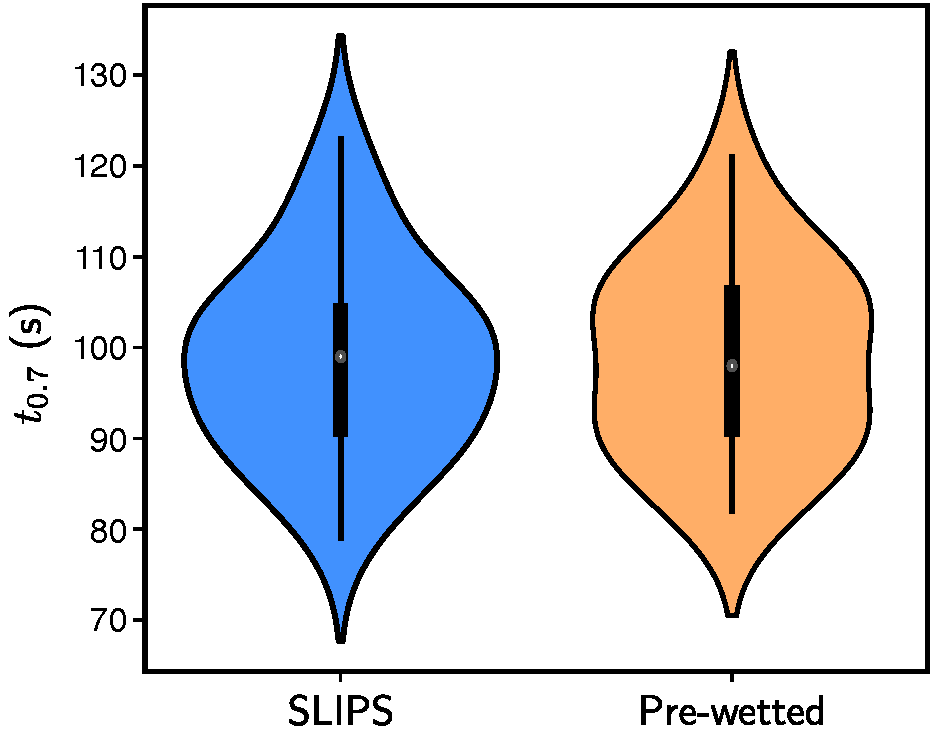
\includegraphics[scale=0.45]{SLIPS_vs_Prewet}
\caption{Violin plot of experimentally obtained values of $t_{0.7}$ for channels prepared with walls treated to achieve a SLIPS (left) and a pre-wetted surface (right). The data are obtained by performing the bendotaxis experiment repeatedly (25 times for SLIPS and 20 times for pre-wetted) using droplets V50 silicone oil droplets of volume $\Omega = 15~\si{\micro}$L in a channel with geometry as follows: $L = 27$~mm, $2H = 430~\si{\micro}$m, $w = 5$~mm, $b = 180~\si{\micro}$m. The mean values are $t_{0.7} = 98.85$~s and $t_{0.7} = 98.89$~s in the SLIPS and pre-wetted cases,
respectively, with standard deviations of $10.8$~s and $10.6$~s.  }\label{fig:Ch3:Appendix:SLIPSvsPrewet}
\end{figure}

To ascertain whether there was any difference between the dynamics of droplets in channels with pre-wetted and SLIPS walls, we performed the bendotaxis experiment repeatedly (25 times in a channel whose walls had been treated to be SLIPS, and 20 times in channels whose walls had been prewetted). The channel geometry was fixed as follows: $L = 27~\si{\milli \meter}$, $2H = 430~\si{\milli \meter}$, $w = 5~\si{\milli \meter}$, $b= 180~\si{\milli \meter}$. We used V50 silicone oil droplets of volume $\Omega = 15~\si{\micro \liter}$; small variations in thickness of the separator -- and hence channel thickness $2H$ -- as well as the volume of liquid we were able to get into the channel, meant that the relative volume $V$ varied in the interval $0.29 < V < 0.35$ (mean $0.32$, standard deviation $0.02$).

Figure~\ref{fig:Ch3:Appendix:SLIPSvsPrewet} shows violin plots~\citep{Hintze1998AmStat} of the values of $t_{0.7}$ for both cases; the kernel density estimates have very similar shapes about an identical mean $t_{0.7} = 98.9~
\si{\second}$. There is no significant difference in $t_{0.7}$ between the two treatments (SLIPS and pre-wetting) and we therefore conclude that the dynamic behaviour in our experimental study of bendotaxis is independent of the choice of surface treatment.

Note that we use the standard deviation in the SLIPS experiments as the error bar included in Figure~\ref{fig:Ch3:RawT23} and Figure~\ref{fig:Ch3:Appendix:tpt7_withNW}.


\section{Non-wetting configurations}\label{Appendix:Ch3:NonWetting}
In this appendix, we describe a suite of bendotaxis experiments performed in non-wetting configurations.
\subsection{Modifications to the experiment}
The experimental setup and protocol is identical to that described in \S3.1 except for two important changes.

Firstly, we used only a SLIPS treatment on the channel walls. We used V5 silicone oil as the lubricating liquid (rather than V50 in the wetting case); this lower viscosity lubricating liquid ensures that the dissipation in the lubricating layer is negligible in comparison with dissipation in the droplet (see Appendix~\ref{Appendix:Ch3:SurfaceCoating}).

The second modification is the use of a glycerol-water mix (GWM) for the droplets. The kinematic viscosity was measured
using a viscometer (Ametek Brookfield, UK) to be $30\pm5~\text{mm\textsuperscript{2}~s\textsuperscript{-1}}$. The density of the GWM was measured to
be $1.196~\text{kg~m\textsuperscript{-3}}$ using a densiometer (DMA 35, Anton Paar GmbH, Austria), from which we calculate a dynamic viscosity of $\mu = 35.9~\textsf{mPa~s}$. The air-liquid surface tension coefficient of the GWM was measured using the pendant drop method~\citep{Stauffer1965Pendant} to be $\gamma = 67~\textsf{mN~m\textsuperscript{-1}}$ (this value is in agreement with previously reported values~\citep{Takamura2012JPetSci}).

We measured the equilibrium contact angle of a $15~\si{\micro} \si{\L}$ droplet of GWM on a single, horizontal SLIPS infused with V5 silicone oil (i.e.~not within a channel) to be $\theta_e = 102\pm 1\si{\degree}$. This was determined by analyzing images taken with a microscope using the ImageJ contact angle plug-in~\citep{Schneider2012}. Errors in this calculation may be significant since the fit does not account for the lubricant skirt, which has a similar refractive index to the GWM. Further, it has been reported~\citep{Schellenberger2015SoftMatter} that microscopic contact angles on SLIPS can vary significantly from those obtained with the elliptic fit technique, while the use of an image of a droplet on a single SLIPS, rather than a channel makes the role of the skirt difficult to quantify. Using the same elliptical fit technique, we measured the advancing and receding contact angles of the droplet moving under gravity on a plate inclined by $1\si{\degree}$ to be $101.8\pm1.7\si{\degree}$ and $100.2\pm2.2\si{\degree}$, respectively.

\subsection{Results}
\begin{figure}[t]
\centering
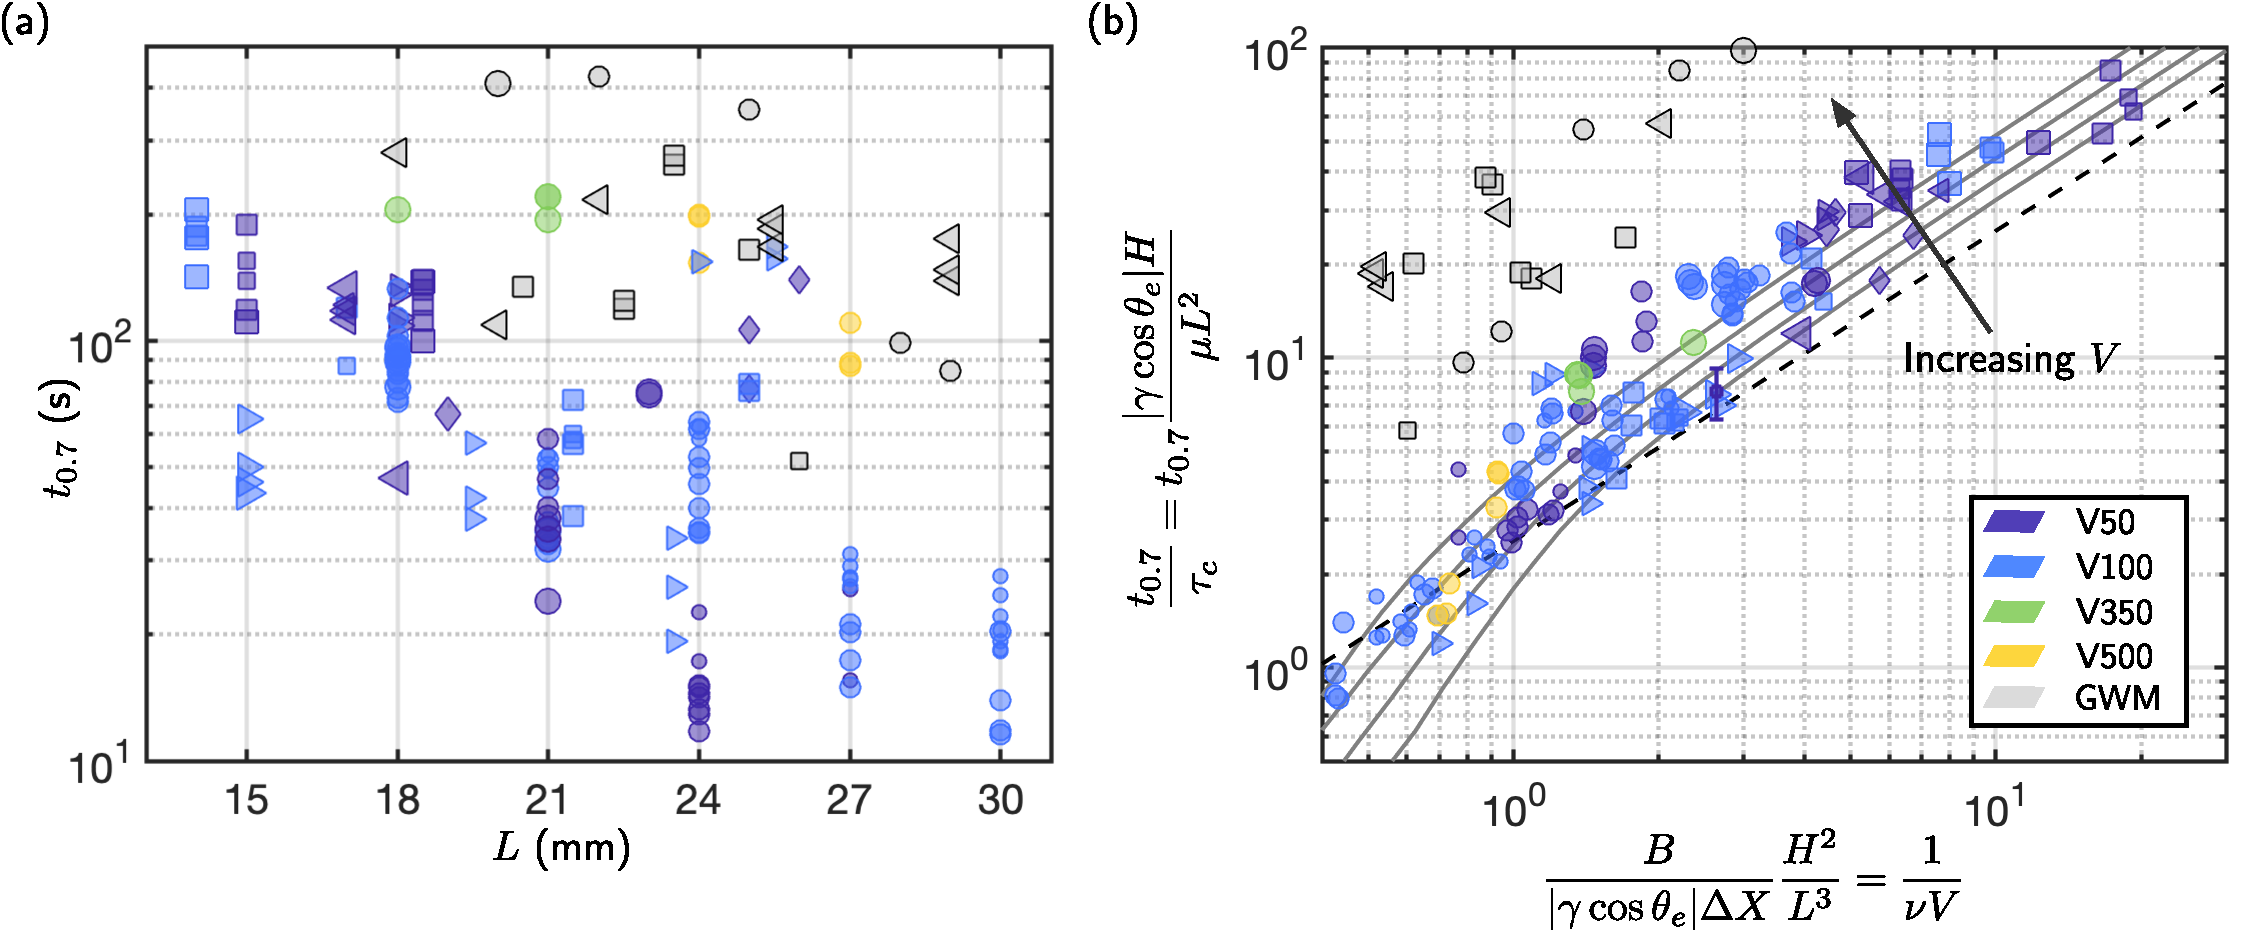
\includegraphics[width = \textwidth]{tpt7_both_with_NW}
\caption{ Raw experimental measurements of $t_{0.7}$ for different channel lengths. The legend in (b) indicates the liquid used (and hence the viscosity and wetting conditions, see main text). Shape and size of the data points encode channel width $2H$ and relative volume $V$, as in Figure~\ref{fig:Ch3:ExptSetup}. (b) Collapse of the experimental data when rescaled according to~\eqref{E:Ch3:ScalingFunctionalForm_asymptotic}. A single set of error bars extends one standard deviation away from a particular data point, computed from 20 measurements (see Appendix~\ref{Appendix:Ch3:SurfaceTreatment:Comparison}). Solid curves show results from numerical solutions of the equations governing the model. Also plotted is the asymptotic result~\eqref{E:Ch3:ScalingFunctionalForm_asymptotic} (including the corresponding pre-factor), valid for $V \ll 1$ (corresponding to the upper right corner of this plot).}\label{fig:Ch3:Appendix:tpt7_withNW}
\end{figure}

The non-wetting experiment was performed a total of 20 times, in channels whose geometry spanned the range described in \S\ref{S:Ch3:ExperimentalSetup:ParameterStudy}.

In Figure~\ref{fig:Ch3:Appendix:tpt7_withNW} we present the raw and rescaled measurements of $t_{0.7}$ from all experiments (i.e.~with both wetting and non-wetting experiments included). The raw experimental data indicate that droplets in non-wetting experiments generally take a longer time than droplets in wetting experiments to traverse the final 30\% of the channel, although the order of magnitude is similar (Figure~\ref{fig:Ch3:Appendix:tpt7_withNW}(a)). The dependence on the channel length is not visible for the data from non-wetting experiments, as it was for the wetting experiments.

When rescaled according to the scaling argument~\eqref{E:Ch3:ScalingFunctionalForm_scaling}, the data from non-wetting experiments show two families with a similar scaling trend but modified pre-factors. We believe that differences between the effective value of $|\gamma \cos \theta_e|$ between measurements made on a single SLIPS and experiments in a narrow channel may be responsible. In addition, droplets may be entirely coated, or `cloaked', by lubricant~\citep{McHale2019Langmuir}, in which case the air-liquid surface tension coefficient is not the correct one to use for the Laplace pressure; we believe that the two families correspond to whether the droplet is cloaked by lubricant or not. It is worth noting that the discrepancy in the pre-factor of the two families can be eliminated by a relatively small change in the effective contact angle of approximately $7\si{\degree}$ and $12\si{\degree}$, for the two families.

\end{subappendices}
}
\graphicspath{{./Sections/Chapter4_finalstates/figures/}}
\chapter{Trapped droplets}

In the model of bendotaxis presented thus far, droplets typically continue to move until one meniscus reaches the free end of the channel. In this chapter, we consider two phenomena that can prevent the droplet from doing so. We devote a section to each: in the first section, we consider the scenario in which the channel walls touch before the droplet has reached the free end, thereby trapping it in a closed channel; we refer to this scenario as geometric trapping. In the second section, we consider the possibility that the contact angles at each meniscus may differ -- the system has contact angle hysteresis; when sufficiently strong, contact angle hysteresis may cause droplets to be trapped in an equilibrium part way along the channel.

Throughout this chapter, the notation introduced in Chapter 2 is assumed and all variables are dimensionless.

\section{Geometric trapping}\label{S:Ch4:Geometric}
%model breaks down when nu big enough as we saw
The mathematical model developed in Chapter 2 relies on the free boundary condition applied at $x = 1$; if the channel walls make contact, this boundary condition is no longer appropriate. This is expected to occur when the bendability $\nu$ is sufficiently large (physically, when surface tension is strong, or the channel walls are compliant); indeed contact is observed in numerical solutions of the model equations (at which point we were terminated the simulation) in \S2.2 and, in \S2.4, we described  how the smallest value of $\nu$ at which wall contact during a simulation occurs depends on the other system parameters, namely the dimensionless volume $V$ and initial droplet position $\xright^0$. In this section, we extend the model of Chapter 2 to describe the system beyond the point at which the channel walls make contact (i.e. beyond the point at which droplets are trapped by the channel geometry), and describe the characteristic behaviour observed in numerical solutions of the equations governing this updated model.

\subsection{Extended theoretical model}\label{S:Ch4:Geometric:Model}
\begin{figure}[t]
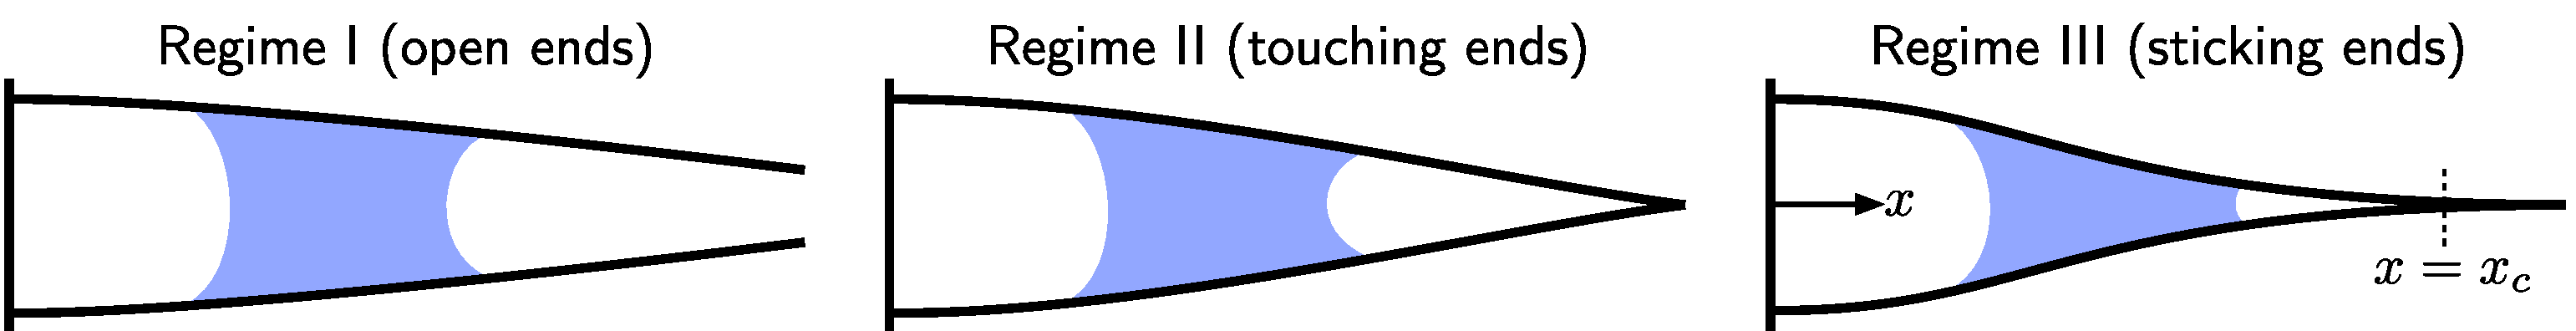
\includegraphics[width = \textwidth]{regime_schematics}
\caption{Schematic diagrams of the possible configurations of a droplet in a deformable channel that is clamped at one end: (a) open ends, (b) touching ends, and (c) sticking ends. We refer to these configurations as regime I, II and III, respectively. }\label{fig:Ch4:Geometric:RegimeSchematics}
\end{figure}

%so what happens beyond touching? introduce the idea of touching and sticking (and their names: regime II and regime III)
There are two cases for walls in contact with one another, as discussed by~\cite{Taroni2012JFM} for the case of an immobile droplet that remains in contact with the clamped end. In the first case, the channel walls make contact at a single point (they `touch', as we encountered in \S2.2). Following~\cite{Taroni2012JFM}, we refer to a channel with touching walls as being in regime II. The second case occurs when surface tension is very strong, causing the slope of the walls at the contact point to reach zero. The channel walls will make contact over a portion of their length (or `stick' together); we refer to channels with sticking walls as being in regime III. Channels whose walls are not in contact (they are `open') are referred to as being in regime I. The different possible configurations are illustrated in Figure~\ref{fig:Ch4:Geometric:RegimeSchematics}.

The model developed in Chapter 2 assumed that channels remain in regime I; to allow us to consider regimes II and III, we allow boundary conditions imposed on the channel shape at the non-clamped end (previously referred to as the free end) to change dynamically. Recall that while the channel remains in regime I, the ends are free and the appropriate boundary conditions are
\abeqn{E:Ch4:Geometric:Model:Regime1_bc}{
\ddp{^3 h}{x^3} = 0, \quad  \ddp{^2 h}{x^2} =0 \quad \text{at}~x = 1. }
Regime I applies while the channel walls remain open, i.e.
\begin{equation}\label{E:Ch4:Geometric:Model:Regime1_necessary_conditions}
h(x = 1,t) > 0.
\end{equation}
Note that our choice of an undeformed initial condition, $h(x,t = 0) = 1$, means that the channel necessarily begins in regime I.

If the walls touch during the motion, so that $h(x =1,t) = 0$ at some point, the channel enters regime II; the channel walls are no longer free at $x = 1$, but exert an equal and opposite reaction force on one another to prevent inter-penetration. We therefore replace the shear free condition~\eqref{E:Ch4:Geometric:Model:Regime1_bc}a by a contact condition. The zero moment boundary condition~\eqref{E:Ch4:Geometric:Model:Regime1_bc}b still applies; the boundary conditions imposed on channels in regime II are
\abeqn{E:Ch4:Geometric:Model:Regime2_bc}{
h = 0, \quad  \ddp{^2 h}{x^2} =0 \quad \text{at}~x = 1. }

The channel remains in regime II provided that the reaction force is repulsive (corresponding to a positive shear force), and that the slope at the contact point remains negative,
\abeqn{E:Ch4:Geometric:Model:Regime2_necessary_conditions}
{\left.\ddp{^3 h}{x^3}\right|_{x = 1} > 0, \quad \left.\ddp{h}{x}\right|_{x = 1} < 0.}
If the repulsive shear condition~\eqref{E:Ch4:Geometric:Model:Regime2_necessary_conditions}a is violated, the channel walls must open, and we return to regime I boundary conditions~\eqref{E:Ch4:Geometric:Model:Regime1_bc} (while we allow for this possibility in our numerics, we have never observed it).

If the negative slope condition~\eqref{E:Ch4:Geometric:Model:Regime2_necessary_conditions}b is violated, then the walls come into contact over a portion of their length, $x_c < x <  1$ (see Figure~\ref{fig:Ch4:Geometric:RegimeSchematics}), where $x_c > \xright$ is the location of the (a priori unknown) first point of contact between the channel walls. (We refer to this case as sticking ends since the walls appear stuck in portion $x_c <x <1$, though we emphasize that there is no adhesive force between them.) In this case, we impose smooth contact conditions at the contact point:
\abceqn{E:Ch4:Geometric:Model:Regime3_bc}{
h = 0, \quad \ddp{h}{x} = 0, \quad \ddp{^2 h}{x^2} = 0 \qquad \text{at}~x = x_c.}
and enforce a flat contact over the section of the channel walls in contact,
\begin{equation}
h = 0, \quad \ddp{h}{x} = 0 \qquad\text{for}~x_c < x < 1.
\end{equation}
Note that~\eqref{E:Ch4:Geometric:Model:Regime3_bc}c imposes an adhesion free contact between the beams~\citep{Kim2006JFM, Majidi2007MechRes} and that this additional boundary condition is necessary to determine the contact point $x_c$ as part of the solution. Channels remain in regime III while the contact point is between the `$+$' meniscus and the wall end,
\begin{equation}
\xright < x_c < 1.
\end{equation}
If $\xright$ reaches $x_c$  our model is no longer valid. If $x_c$ increases to beyond $x = 1$, the channel returns to regime II (again, this transition is allowed for in our numerics, but has not been observed).

The PDE~\eqref{E:Chapter2:Model:NonDim:CombinedEq1}--\eqref{E:Chapter2:Model:NonDim:CombinedEq3} describing the channel width,
\begin{align}
0 &= \ddp{^4 h}{x^4} & &0 < x < \xleft,\label{E:Ch4:Geometric:Model:flow_eq1}\\
\ddp{h}{t} &= \frac{1}{3|\nu|}\ddp{}{x}\left(h^3 \ddp{^5 h}{x^5}\right) & &\xleft < x <\xright, \\
0 &= \ddp{^4 h}{x^4} & &\xright < x < 1,\label{E:Ch4:Geometric:Model:flow_eq3}
\end{align}
still applies, as do the kinematic conditions~\eqref{E:Chapter2:Model:NonDim:Kinematic},
\begin{equation}\label{E:Ch4:Geometric:Model:kinematic}
\dd{x_{\pm}}{t} = -\left.\frac{h^2}{3|\nu|}\ddp{^5 h}{x^5}\right|_{x = x_{\pm}}.
\end{equation}
The boundary conditions at $x = 0$ and $x = x_{\pm}$ are as in Chapter 2 (\eqref{E:Chapter2:Model:NonDim:BCClamped}, \eqref{E:Chapter2:Model:NonDim:BCContinuity}, and~\eqref{E:Chapter2:Model:NonDim:BCPressure}); the complete set of boundary conditions for~\eqref{E:Ch4:Geometric:Model:flow_eq1}--\eqref{E:Ch4:Geometric:Model:flow_eq3} are summarised in Table~\ref{T:Ch4:Geometric:BoundaryConditions}.

\begin{table}[t!]
 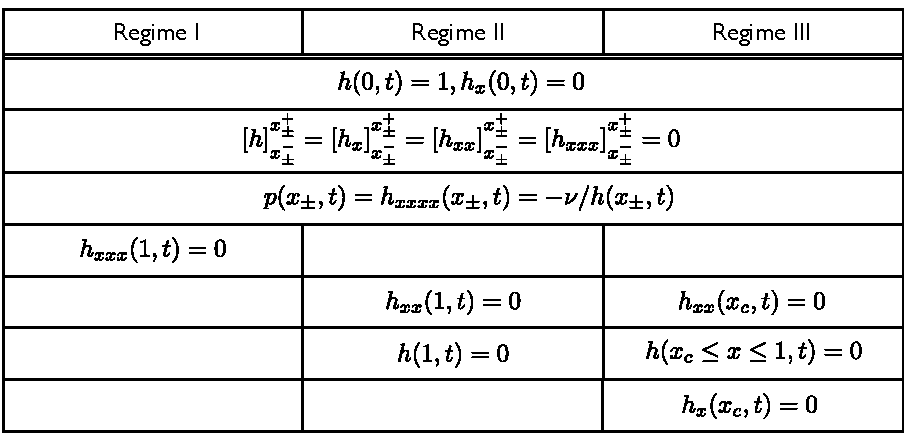
\includegraphics[scale = 0.99]{table_of_bc}
   \caption{Boundary conditions on the PDE~\eqref{E:Ch4:Geometric:Model:flow_eq1}--\eqref{E:Ch4:Geometric:Model:flow_eq3} that describes the coupled channel deflection and droplet motion in a flexible channel with either open ends (regime I), touching ends (regime II), or sticking ends (regime III). Note that subscript $x$ denotes a partial derivative in this table.}  \label{T:Ch4:Geometric:BoundaryConditions}
\end{table}

Also as in Chapter 2, we use the initial conditions
\begin{equation}\label{E:Ch4:Geometric:Model:IC}
h(x, 0) = 1,\quad \xright(0) = \xright^0, \quad \xleft(0) =\xleft^0 =  \xright^0 - V,
\end{equation}
ensuring that the dimensionless droplet volume is $V$. We note that equilibria are not possible in any of regimes I--III, because an equilibrium would require an equal channel width at both sides of the droplet.

\subsection{Numerical solutions}
To illustrate the numerical solution of the model equations (equations~\eqref{E:Ch4:Geometric:Model:flow_eq1}--\eqref{E:Ch4:Geometric:Model:IC} alongside the appropriate choice of~\eqref{E:Ch4:Geometric:Model:Regime1_bc},~\eqref{E:Ch4:Geometric:Model:Regime2_bc}, or~\eqref{E:Ch4:Geometric:Model:Regime3_bc}) we consider the cases of $\nu = 30$ and $\nu = 100$ (with $V = 0.3$, $\xright^0 = 0.4$ in each case). We shall see that with $\nu  = 30$, the simulation reaches regime II but not regime III and the simulation with $\nu = 100$ terminates while the channel is in regime III.

\subsubsection{Modifications to numerical scheme}\label{S:Geometry:Numerics}
Before presenting the dynamics of the numerical solutions, we briefly discuss the two modifications that must be made to the numerical scheme described in \S2.2.1 to implement regime II and III boundary conditions~\eqref{E:Ch4:Geometric:Model:Regime2_bc} and~\eqref{E:Ch4:Geometric:Model:Regime3_bc}, as well as dynamic changes between regimes.

\paragraph{Modification 1: isolating the drop region.}  Recall that the first step in the numerical scheme is to express the shape of the channel in the dry regions $0 < x <\xleft$ and $\xright < x < 1$ in terms of the channel shape in the drop region $\xleft < x < \xright$.  For the region $0 < x <\xleft$, we  solve~\eqref{E:Ch4:Geometric:Model:flow_eq1} alongside the clamped conditions~\eqref{E:Chapter2:Model:NonDim:BCClamped} and continuity conditions \eqref{E:Chapter2:Model:NonDim:BCContinuity}a,b;  imposing the other two continuity conditions, \eqref{E:Chapter2:Model:NonDim:BCContinuity}c,d, then results in the effective boundary conditions~\eqref{E:Chapter2:Numerics:SchemE:Chapter2:Reduced:EffectiveBCLower}, independently of the conditions at the non-clamped end. For the region $\xright < x < 1$, we solve~\eqref{E:Ch4:Geometric:Model:flow_eq3} alongside~\eqref{E:Chapter2:Model:NonDim:BCContinuity}a,b and the appropriate choice of~\eqref{E:Ch4:Geometric:Model:Regime1_bc},~\eqref{E:Ch4:Geometric:Model:Regime2_bc}, or~\eqref{E:Ch4:Geometric:Model:Regime3_bc}. Imposing the continuity conditions~\eqref{E:Chapter2:Model:NonDim:BCContinuity}c,d is then equivalent to imposing effective boundary conditions at $x = \xright$ that encode the effect of the adjacent dry region.

The channel shape in the dry region $\xright < x < 1$ (and thus effective boundary conditions applied at $x = \xright$ on the drop-only problem) must be adjusted to reflect the possible boundary conditions at the non-clamped end. Recall that for regime I configurations, the shape in the dry region $\xright < x < 1$ is expressed in terms of the shape in the drop region as
\begin{equation}
h(x,t) = \left.\ddp{h}{x}\right|_{x = \xright}(x - \xright) + \left.h\right|_{x = \xright} \qquad \xright < x <1,
\end{equation}
and the resulting effective boundary conditions are
\begin{equation}
\ddp{^2 h}{x^2} = 0, \quad \ddp{^3 h}{x^3} = 0 \quad \text{at}~x = \xright.
\end{equation}

In regime II, the channel shape in the dry region may be expressed in terms of the shape in the drop region as
\begin{multline}\label{E:Ch4:Geometric:Numerics:DryShapeRegimeII}
h(x,t) =\frac{1}{2}\left.\left[3 h + (1 -\xright)\ddp{h}{x}\right]\right|_{x = \xright} \left(\frac{1-x}{1-\xright}\right)-\\ \left.\frac{1}{2} \left[h + (1- \xright) \ddp{h}{x}\right]\right|_{x = \xright}\left(\frac{1-x}{1-\xright}\right)^3 \qquad \xright < x < 1.
\end{multline}
The resulting effective boundary conditions are
\begin{equation}
\ddp{^2 h}{x^2} = \frac{-3}{(1 - \xright)^2}\left[h + (1-\xright) \ddp{h}{x}\right],\quad \ddp{^3 h}{x^3}  =  \frac{3}{(1-\xright)^3}\left[h + (1-\xright) \ddp{h}{x} \right]
\end{equation}
at $x = \xright$.

For channels in regime III, the channel shape in the dry region is
\begin{equation}\label{E:Ch4:Geometric:Numerics:DryShapeRegimeIII}
h(x,t) = \left.h\right|_{x = \xright} \left(\frac{x_c - x}{x_c - \xright}\right)^3 \qquad \xright < x < x_c
\end{equation}
where
\begin{equation}
x_c = \xright - 3  \left.h\right|_{x = \xright} \left(\left.\ddp{h}{x}\right|_{x = \xright}\right)^{-1}.
\end{equation}
The effective boundary conditions are
\begin{equation}
\ddp{^2 h}{x^2} = \frac{6h}{(x_c - \xright)^2}, \quad \ddp{^3 h}{x^3}  = \frac{6h}{(x_c - \xright)^3} \quad \text{at}~x = \xright.
\end{equation}

\begin{figure}[t]
\centering
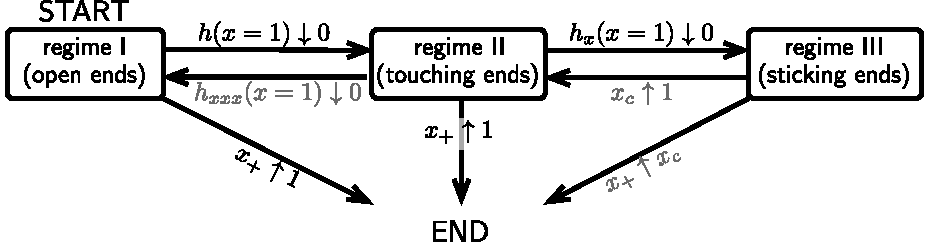
\includegraphics[scale=0.9]{geometric_numerics_events}
\caption{Flowchart of the dynamic events that trigger either a change in boundary conditions or the termination of the integration in numerical solutions of the model equations. The arrow labels indicate the event function that triggers the associated regime change or ends the simulation, and up (down) arrows indicate that the function must increase (decrease, respectively) through the value. Grey labels indicate those events that are included in the model, but are never triggered.}\label{fig:Ch4:Geometric:Flowchart}
\end{figure}

\paragraph{Modification 2: dynamically adjusting the boundary conditions.} The second  modification to the numerical scheme described in \S2.2.1 is to allow the effective boundary conditions to change dynamically. At each time-step, we determine whether changes in the boundary conditions applied at $x = x_{\pm}$ are needed, or whether the numerical integration should terminate, by evaluating event functions that indicate these transitions. These event functions, and the transitions that they trigger, are summarized in Figure~\ref{fig:Ch4:Geometric:Flowchart}. Note that in practice, we terminate the integration when the appropriate event function ($1 - \xright$ for channels in regime II, and $x_c - \xright $ for channels in regime III) comes within some tolerance of zero (we use a tolerance of $10^{-3}$ in the simulations presented here); by terminating the simulations `early', we avoid a singularity in the droplet pressure as the `$+$' meniscus advances into a channel with vanishing thickness.


\subsubsection{Dynamics}
\begin{figure}[h!]
\centering
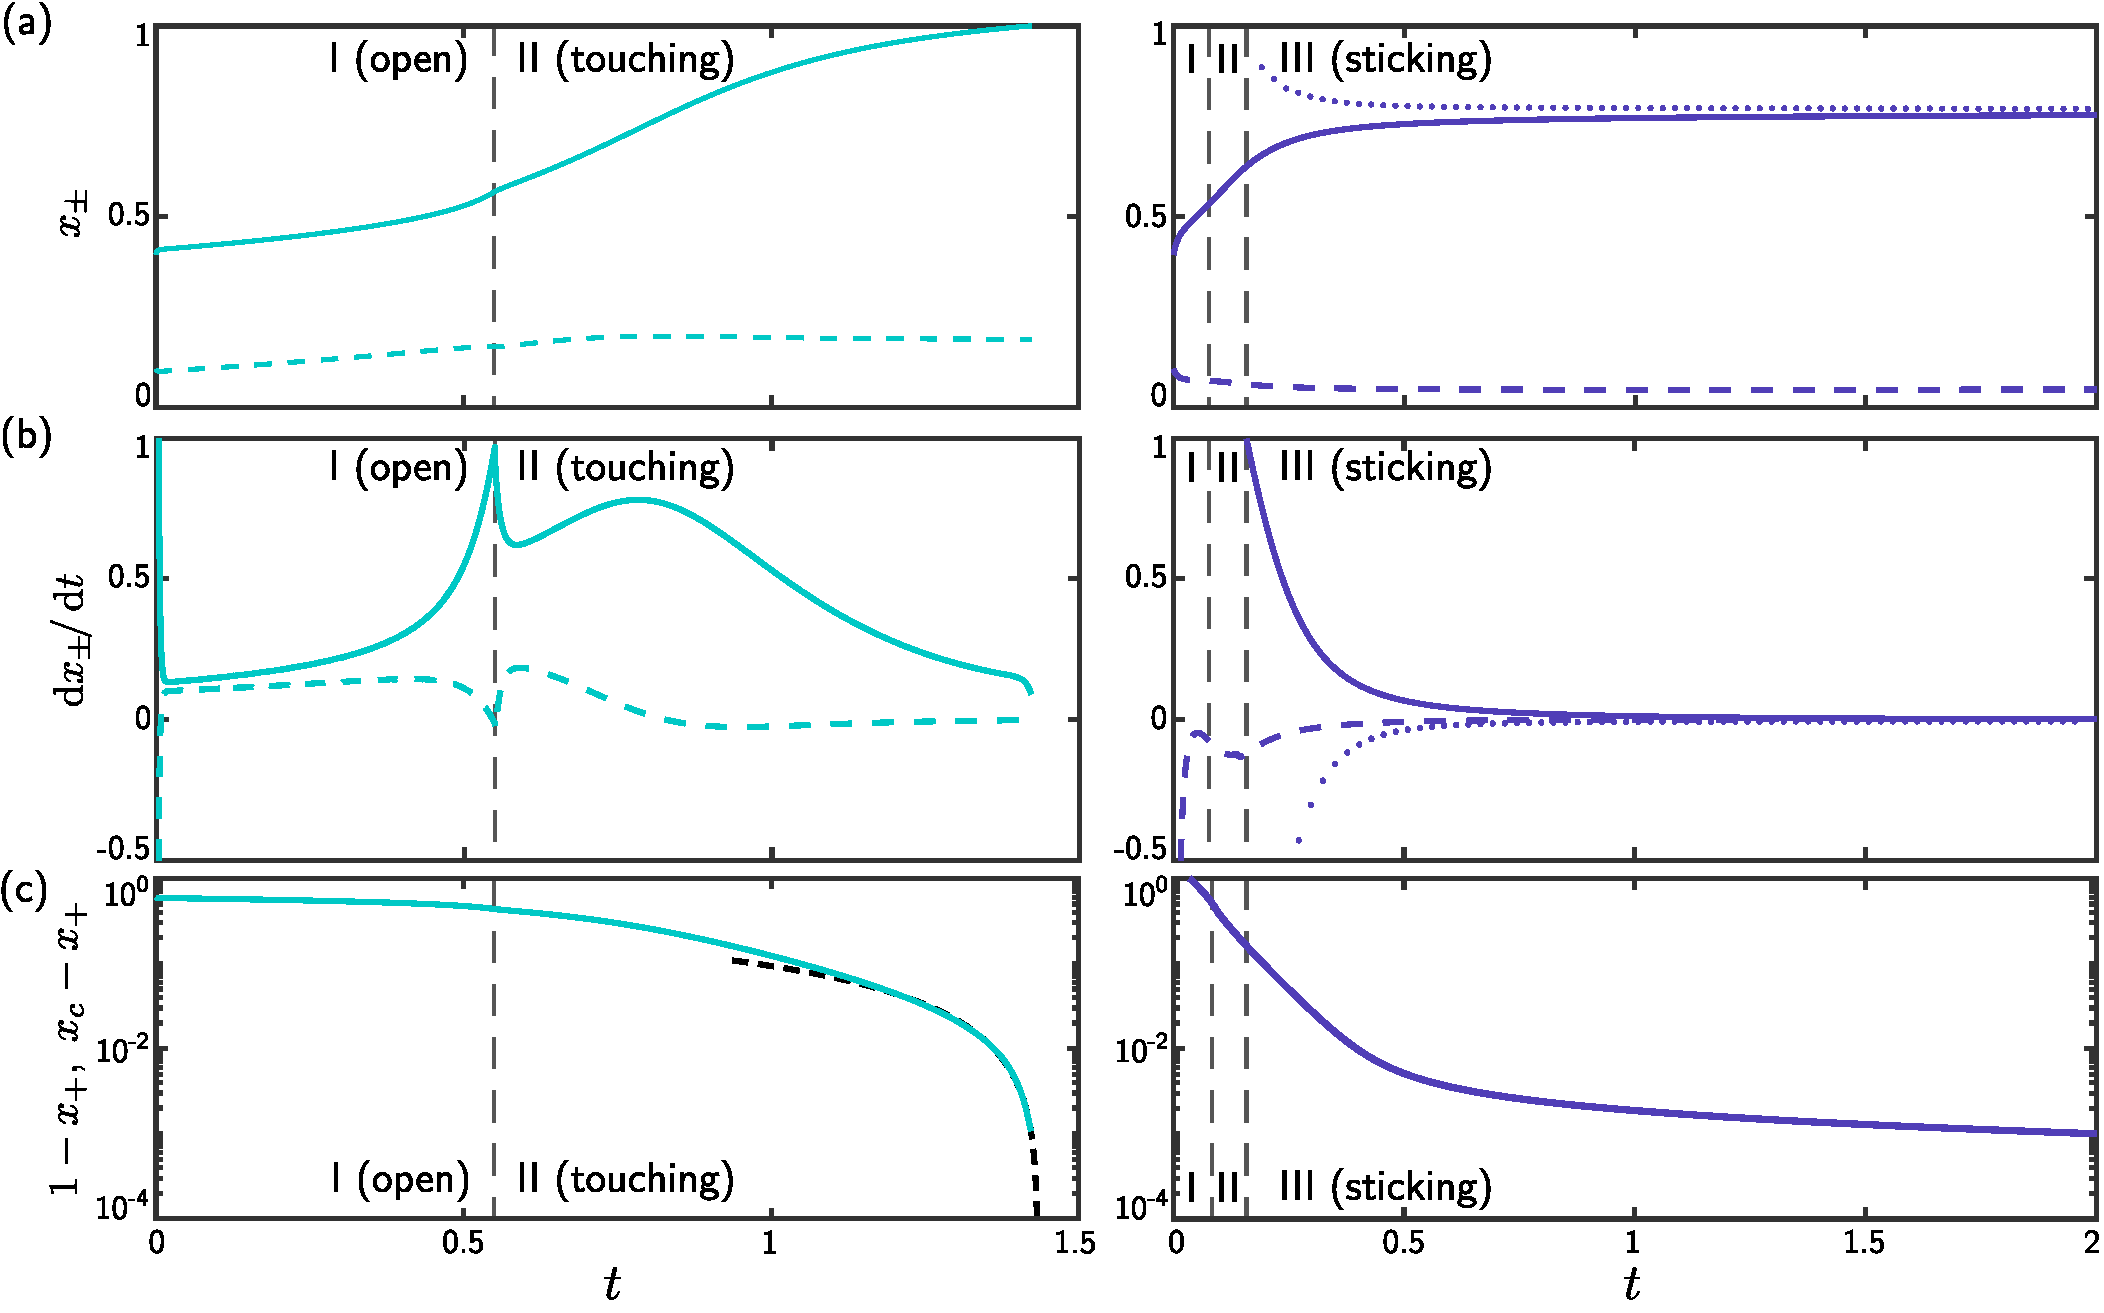
\includegraphics[width=\textwidth]{touching_and_sticking_traces}
\caption{Numerical solutions in which the system is allowed to change regimes. (a) Meniscus trajectories and (b) meniscus velocities obtained by numerically solving the model equations for $\nu = 30$ (left) and $\nu  = 100$ (right) (both solutions have $\xright^0 = 0.4$, $V = 0.3$ and use $200$ grid points). Solid and dashed curves indicate the `$+$' and `$-$' menisci, respectively; where applicable, dotted curves indicate the contact point $x_c$. (c) Plot of distance of the meniscus to the channel closure: for regimes I and II configurations (left) this is $1 - \xright$, for regime III configurations, this is $x_c - \xright$. The black dashed curve indicates the fit~\eqref{E:Ch4:Geometric:numerics:contact_time}. Vertical dashed lines indicate transitions between the various contacting conditions.}\label{fig:Ch4:geometric:numerics}
\end{figure}

Examples of the dynamic behaviour determined from the numerical solution of the model equations (allowing for changes between regimes I-III) are shown in Figure~\ref{fig:Ch4:geometric:numerics}. The left panel of Figure~\ref{fig:Ch4:geometric:numerics} shows a scenario in which the system transitions from regime I to II but appears to remain in II as $\xright \to 1$ (i.e. it does not transition to regime III). In this case, the movement of the droplet in regime I (prior to walls contacting) is dominated by translating rather than spreading -- the menisci both move in the same direction. Immediately prior to contact there is a brief spreading phase in which the leading meniscus accelerate and the rear meniscus retreats ($\mathrm{d}\xleft/\mathrm{d}t < 0$). This is reversed immediately after the contact followed by a phase in which the leading meniscus moves (at a decelerating rate) towards the contact point while the rear meniscus is approximately stationary.

By comparison, the dynamics of a system that reaches regime III are relatively simple (see right panels of Figure~\ref{fig:Ch4:geometric:numerics}).   The channel is in both regime I and II for a relatively short period of time. Throughout the motion, the `$+$' meniscus is decelerating from the high initial velocity that is a consequence of the strong early squeezing. The majority of the time is spent with the channel in regime III and $\xright$ close to $x_c$.

\subsubsection{Contact time}
%adjust discussion in previous section so we jsut say 'terminates with 1-xu = 1e-3 or xc - xu = 1e-3' discuss what happens beyond this point.
Both the simulation with $\nu = 30$  and that with $\nu = 100$ terminate when the meniscus gets within the tolerance ($10^{-3}$) of the channel end. Even with this caveat,  the curvature of the traces of $1 - \xright$ and $x_c - \xright$, shown in Figure~\ref{fig:Ch4:geometric:numerics}(c), suggest that the the meniscus would reach the channel end in finite time in the regime II case ($\nu = 30$) but would not in the regime III case ($\nu = 100$).

We have not been able to rationalize the observations using an analysis of the governing PDE. However, we note that a power law fit of the regime II case suggests that
\begin{equation}\label{E:Ch4:Geometric:numerics:contact_time}
1 - \xright \sim (t_c - t)^{5/4} \quad \text{as}~t_c - t \to 0,
\end{equation}
where $t = t_c$ is the time at which the meniscus reaches the channel end.

It is interesting to compare these results with imbibition in a rigid channel. \cite{Gorce2016Langmuir} showed that the meniscus of a column of liquid imbibing into a tapered channel with a linear profile reaches the taper `corner' linearly in time with $1 - \xright \sim t_c - t$ as $ t_c - t \to 0$ (the same imbibition behaviour was also observed for droplets by~\cite{Reyssat2014JFM}). In the present (deformable) case, the channel has a locally linear profile at the contact point ($x = 1$) when in regime II (see equation~\eqref{E:Ch4:Geometric:Numerics:DryShapeRegimeII}) and appears to make contact in finite time at a faster rate than in the rigid case ($(t_c - t)^{5/4}$ versus $(t_c - t)^1$). We believe that this is because the angle of the tapering in the flexible case may change during the motion.

\cite{Gorce2016Langmuir} also showed that  the meniscus of a column of liquid approaches the tip of a channel with a cubic profile only algebraically slowly, which appears to be in accord with the flexible case here (channels in regime III have a cubic profile near the contact point $x = x_c$, see equation~\eqref{E:Ch4:Geometric:Numerics:DryShapeRegimeIII})


\section{Trapping with hysteresis}
%
\newcommand{\hyspar}{\lambda}
\newcommand{\hysparmax}{\hyspar_{\text{max}} }
\newcommand{\hyspare}{\lambda_e}
\newcommand{\hyspari}{\lambda_{\infty}}
\newcommand{\xlefteq}{X_{-}}
\newcommand{\xrighteq}{X_{+}}
\newcommand{\xceq}{X_{c}} %meniscus poositions in equilibrium
\newcommand{\xpmeq}{X_{\pm}} %collective term for meniscus positions in equilibrium

%in reality non-unique angles
In our modelling so far, we have assumed that the contact angle between the liquid and the channel walls takes the equilibrium, or Young, value $\theta_e$ at both menisci. In reality, the contact angles are non-unique~\citep{deGennes2004}: the contact angle $\theta$ can take any value in the interval $[\theta_r, \theta_a]$ where $\theta_a$ is referred to as the advancing contact angle and $\theta_r$ is referred to as is the receding contact angle.

%what do contact angles look like in practice
A complete description of contact angle hysteresis is beyond the scope of this thesis. In this chapter, we add a simple encoding of contact angle hysteresis to the model developed in Chapter 2 and Section 4.1, which aims to capture the essential behaviour, as described by~\cite{deGennes2004}:
\begin{quote}
If, for instance, we inflate a drop (Figure~\ref{fig:Ch4:Hysteresis:primer}(a)), the contact angle $\theta$ can exceed $\theta_e$ without the line of contact moving at all. Eventually, $\theta$ reaches a threshold value $\theta_a$ beyond which the line of contact finally does move. $\theta_a$ is referred to as the advancing angle.

Likewise, when deflating a drop (Figure~\ref{fig:Ch4:Hysteresis:primer}(a)) $\theta$ can decrease down to a limiting value $\theta_r$, known as the receding angle. When $\theta = \theta_r$, the line of contact suddenly shifts.
\end{quote}
In this Chapter we supplement this static picture with the simplest possible dynamics: $\theta = \theta_a$ if the contact line is advancing and $\theta  = \theta_r$ if the contact line is receding.

Generally, contact angle hysteresis impedes droplet motion. For example, it is contact angle hysteresis that opposes gravity when slugs of liquid remain stationary in vertical capillary tubes. It has also been shown~\citep{Prakash2008Science, Bush2010AdvCollIntsci} that contact angle hysteresis, when sufficiently strong, can  arrest the motion of droplets in tapered channels that were moving as a result of the channel's tapering. We might expect a similar scenario in bendotaxis, where the droplet motion itself results from the tapering of the channel (albeit one that is induced by the droplet itself, rather than externally imposed). In this section, we aim to understand whether this expectation is correct: can contact angle hysteresis prevent droplet motion by bendotaxis? If so, when does hysteresis-induced trapping occur?

\subsection{Modelling hysteresis}\label{S:Ch4:hysteresis:modelling}
\subsubsection{Preliminaries}
\begin{figure}[t]
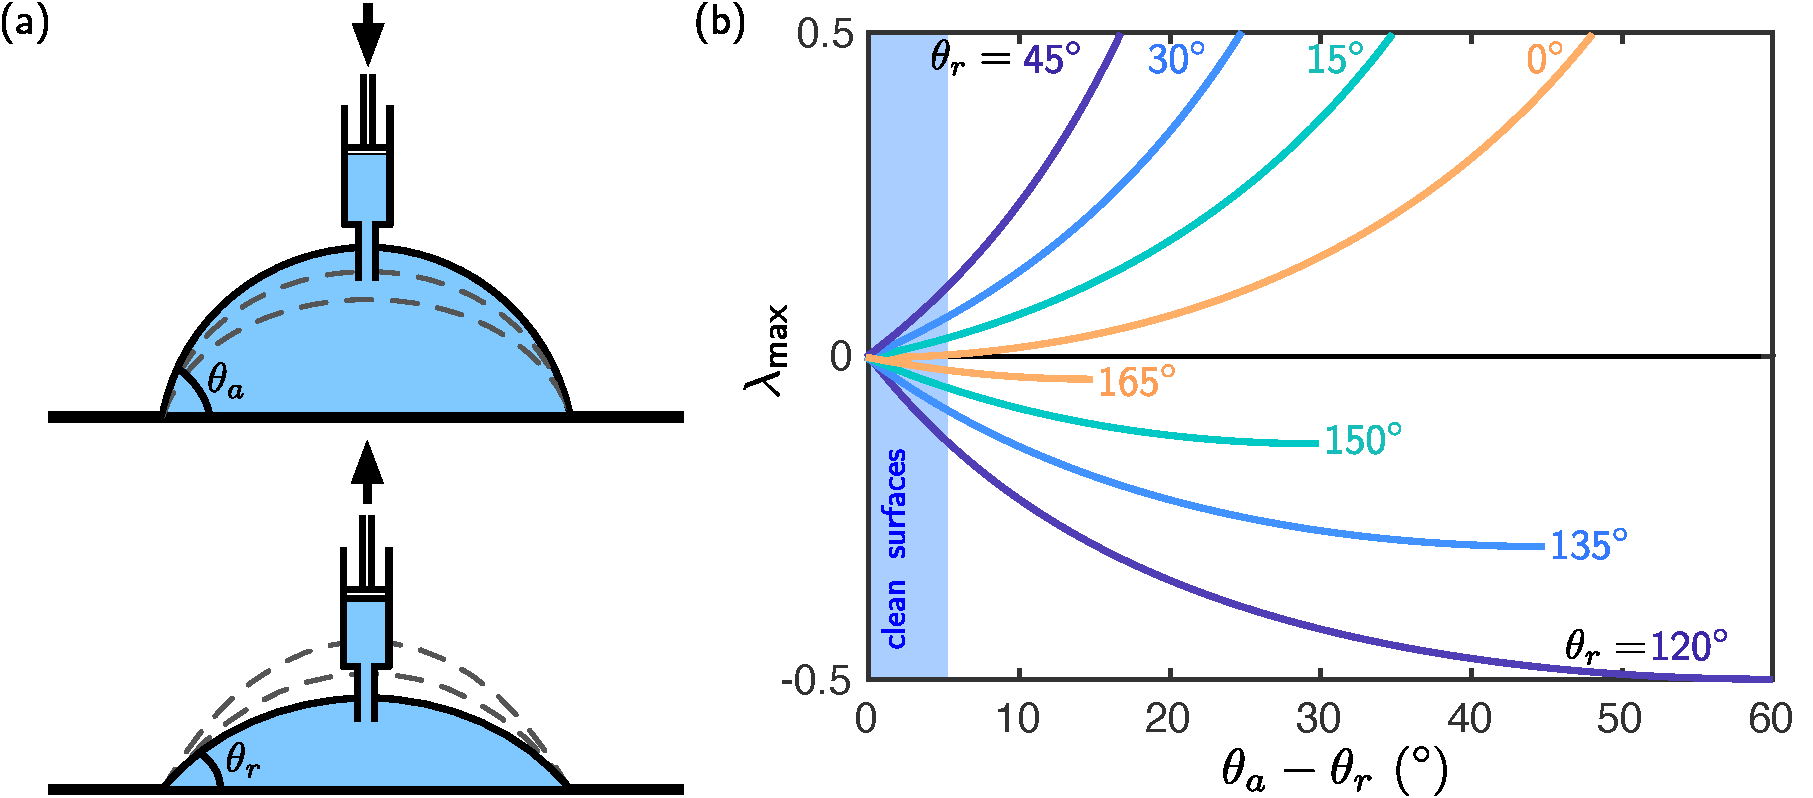
\includegraphics[scale=0.48]{cahys_primer}
\caption{(a) Schematic diagram illustrating the advancing (top) and receding (bottom) contact angles. When a droplet is being quasi-statically inflated the meniscus evolves through increasing contact angles $\theta < \theta_a$ without the contact line moving. Once $\theta = \theta_a$ the contact line advances. Similarly, when a droplet is being quasi-statically deflated, the meniscus evolves through decreasing contact angles $\theta > \theta_r$. Once $\theta = \theta_r$ the contact line recedes. (b) Plot of $\hyspar_{\text{max}}$ (equation~\eqref{E:ch4:Hysteresis:Parametrisation:hyspar_def}) as a function of $\theta_a - \theta_r$ for various receding angles $\theta_r$.  }\label{fig:Ch4:Hysteresis:primer}
\end{figure}

We present a model of contact angle hysteresis that captures the characteristic features of contact angle hysteresis described in the previous section: (i) the droplet-channel system has intrinsic advancing and receding contact angles, $\theta_a$ and $\theta_r$, respectively, with $\theta_a \geq \theta_r$, (ii) an interface is advancing (receding) if and only if the contact angle at the interface is $\theta_a$ ($\theta_r$, respectively) and (iii) the contact angle at a stationary interface may take any contact angle $\theta_r < \theta < \theta_a$.

In our system, the contact angle $\theta$ does not arise alone but rather its cosine does. It is therefore helpful to introduce the parameter
\begin{equation}\label{E:ch4:Hysteresis:Parametrisation:hyspar_def}
\hysparmax = \frac{\cos \theta_r}{\cos \theta_a} - 1
\end{equation}
as a measure of the asymmetry between the advancing and receding angles, or contact angle hysteresis. Assuming that the advancing and receding contact angles lie on the same side of 90$\si{\degree}$ (they correspond to the same wettability), then $\hysparmax >0$ for wetting configurations ($\theta_a < 90\si{\degree}$) and $\hysparmax <0$ for non-wetting configurations ($\theta_a > 90\si{\degree}$).

While this is different from the usual definition of contact angle hysteresis, $\theta_a - \theta_r$, these two measures of hysteresis are closely related:  Figure~\ref{fig:Ch4:Hysteresis:primer}(b) shows that $\hysparmax$ is monotonic in $\theta_a - \theta_r$ (increasing for wetting configurations and decreasing for non-wetting configurations). Increases in $|\hysparmax|$ therefore correspond to increases in $\theta_a - \theta_r$, and, also, $\hyspar_{\text{max}} = 0$ if and only if $\theta_a - \theta_r = 0$ (see Figure~\ref{fig:Ch4:Hysteresis:primer}(b)). Moreover,~\cite{deGennes2004} suggests that surfaces with $\theta_a - \theta_r < 5\si{\degree}$ are relatively clean (shaded in Figure~\ref{fig:Ch4:Hysteresis:primer}(b)); here $|\hysparmax|\ll 1$.

Since the contact angles at the menisci, $\theta_{\pm}(t)$, are now time-dependent, we also define
\begin{equation}\label{E:ch4:Hysteresis:Parametrisation:hyspar_dynamic_def}
\hyspar(t) =  \frac{\cos \theta_-(t)}{\cos \theta_+(t)} - 1,
\end{equation}
as measure of the instantaneous contact angle asymmetry. Within our model, $\hyspar$ has the following properties: (i) $\hyspar \leq \hyspar_{\text{max}}$ for wetting configurations and $\hyspar \geq \hyspar_{\text{max}}$ for non-wetting configurations (we will, therefore, often refer to $\hysparmax$ as the maximum contact angle asymmetry for wetting configurations), (ii)  $\hyspar = 0$ corresponds to $\theta_+ = \theta_-$ (equal contact angles at both menisci) and (iii) $\hyspar = \hyspar_{\text{max}}$ if $\theta_+ = \theta_a$ and $\theta_- = \theta_r$ (as we expect for a droplet moving towards the free end of the channel with `$+$'  meniscus advancing and `$-$' meniscus receding).

Finally, we note that in this framework, the equilibrium contact angle $\theta_e$ is no longer a relevant parameter. We must therefore choose how to replace the factors of $\cos \theta_e$ that appeared in the non-dimensionalization of Chapter 2. In the following, we use $\cos \theta_a$ in place of $\cos \theta_e$, i.e. we let
\begin{equation}\label{E:ch4:Hysteresis:Parametrisation:modified_nu_def}
\tau_c = \frac{\mu L^2}{|\gamma \cos \theta_a|H}, \quad\text{and}\quad \nu = \frac{\gamma \cos \theta_a L^4}{BH^2},
\end{equation}
respectively.

\subsubsection{Modified boundary conditions}
Incorporating this model of contact angle hysteresis into our model simply involves modifying the boundary conditions that apply at $x =x_{\pm}$, and allowing them to change dynamically. There are three cases for each meniscus, depending on its current motion and the contact angle there. Throughout, we keep in mind that the kinematic conditions and Laplace pressure conditions, which now read
\abeqn{E:ch4:Hysteresis:Parametrisation:kbc_and_laplace}{
\dd{x_{\pm}}{t} = \left. \frac{-h^2}{3|\nu|}\ddp{^5 h}{x^5}\right|_{x = x_{\pm}} \quad \text{and} \quad \left.\ddp{^4 h}{x^4}\right|_{x =x_{\pm}} = -\frac{\nu}{h(\xright,t)}\frac{\cos \theta_{\pm}}{\cos \theta_a},}
respectively, always hold.

Consider first the `$+$' meniscus. If this is moving with a positive velocity (corresponding to a negative pressure gradient), it is advancing out of the liquid so $\theta_+ = \theta_a$, i.e. we set
\begin{equation}\label{E:ch4:Hysteresis:Parametrisation:BC+_advancing}
\theta_+ = \theta_a, \qquad \text{if}~\dd{\xright}{t} > 0.
\end{equation}

If the `$+$' meniscus subsequently stops moving (the pressure gradient decreases to zero), it is then pinned in place; its contact angle $\theta_+$ takes the value between $\theta_r$ and $\theta_a$  (via the Laplace pressure condition~\eqref{E:ch4:Hysteresis:Parametrisation:kbc_and_laplace}b) that maintains zero pressure gradient, i.e. we set \begin{equation}\label{E:ch4:Hysteresis:Parametrisation:BC+_pinned}
\theta_r \leq \theta_+ \leq \theta_a \quad \text{if}~\dd{\xright}{t}  = 0.
\end{equation}
Should the contact angle increase back up to $\theta_a$ while the meniscus is pinned, we return to the advancing conditions~\eqref{E:ch4:Hysteresis:Parametrisation:BC+_advancing}. If, on other hand, the contact angle decreases down to $\theta_r$, the meniscus begins to recede into the liquid (it moves with a negative velocity) taking the receding angle, i.e. we set
\begin{equation}\label{E:ch4:Hysteresis:Parametrisation:BC+_receding}
\theta_+ = \theta_r \qquad \text{if}~\dd{\xright}{t} <0.
\end{equation}
The transition from receding back to pinned occurs if the meniscus velocity increases back to zero from below.

The conditions on $\theta_-$ are very similar: precisely one of
\renewcommand*{\arraystretch}{1.3}
\abceqn{E:ch4:Hysteresis:Parametrisation:BC_xleft}{
\left\{
\begin{matrix}
\theta_- = \theta_a & \dd{\xleft}{t} < 0,\\
\theta_r < \theta_- < \theta_a  &\dd{\xleft}{t} =  0,\\
\theta_- = \theta_r & \dd{\xleft}{t} > 0,
\end{matrix} \right.}
must hold at all times. (The small differences between the contact angle conditions on $\theta_+$ and $\theta_-$ are a result of being located on opposite sides of the droplet, so that advancing and receding have opposing senses for the two menisci.)

To close the model, we need to specify initial conditions on the contact angles $\theta_\pm$. To be consistent with the early squeezing, in which the menisci move in opposite directions (away one another for wetting configurations, and towards from one another for non-wetting configurations), we take initial conditions
\begin{equation}\label{E:ch4:Hysteresis:Parametrisation:ic_theta_wetting}
\theta_{\pm}(t = 0) = \theta_a
\end{equation}
for wetting conditions (i.e. if $\hyspar > 0, \nu >0$) and
\begin{equation}
\theta_{\pm}(t = 0) = \theta_r
\end{equation}
for non-wetting conditions ($\hyspar < 0, \nu <0$). Here, we shall focus primarily on wetting conditions, which display more diverse behaviour (the different contacting regimes discussed in \S\ref{S:Ch4:Geometric} are only possible for wetting conditions); we discuss the corresponding results for non-wetting configurations in \S\ref{S:Ch4:Hysteresis:NonWetting}.

\subsection{Numerical Solutions}\label{S:Ch4:Hysteresis:Numerics}

\begin{figure}[t]
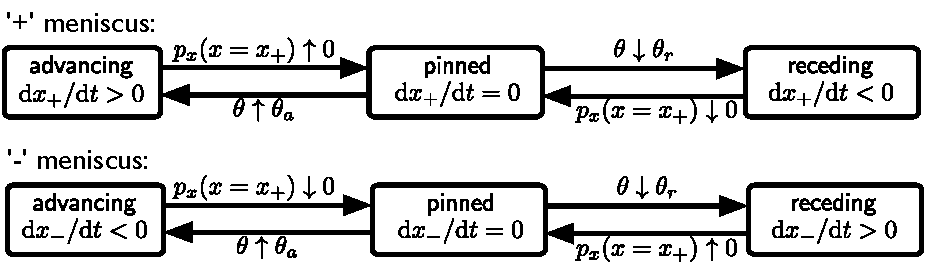
\includegraphics[scale = 0.97]{transitions_contact_angles}
\caption{Flowchart of the dynamic events that result in a change of boundary conditions in the model equations describing bendotaxis with contact angle hysteresis. The arrow labels indicate the function that triggers the transition, and up (down) arrows indicate that the function must increase (decrease, respectively) through the corresponding value.}\label{fig:Ch4:Hysteresis:Flowchart}
\end{figure}

\begin{figure}[h!]
\centering
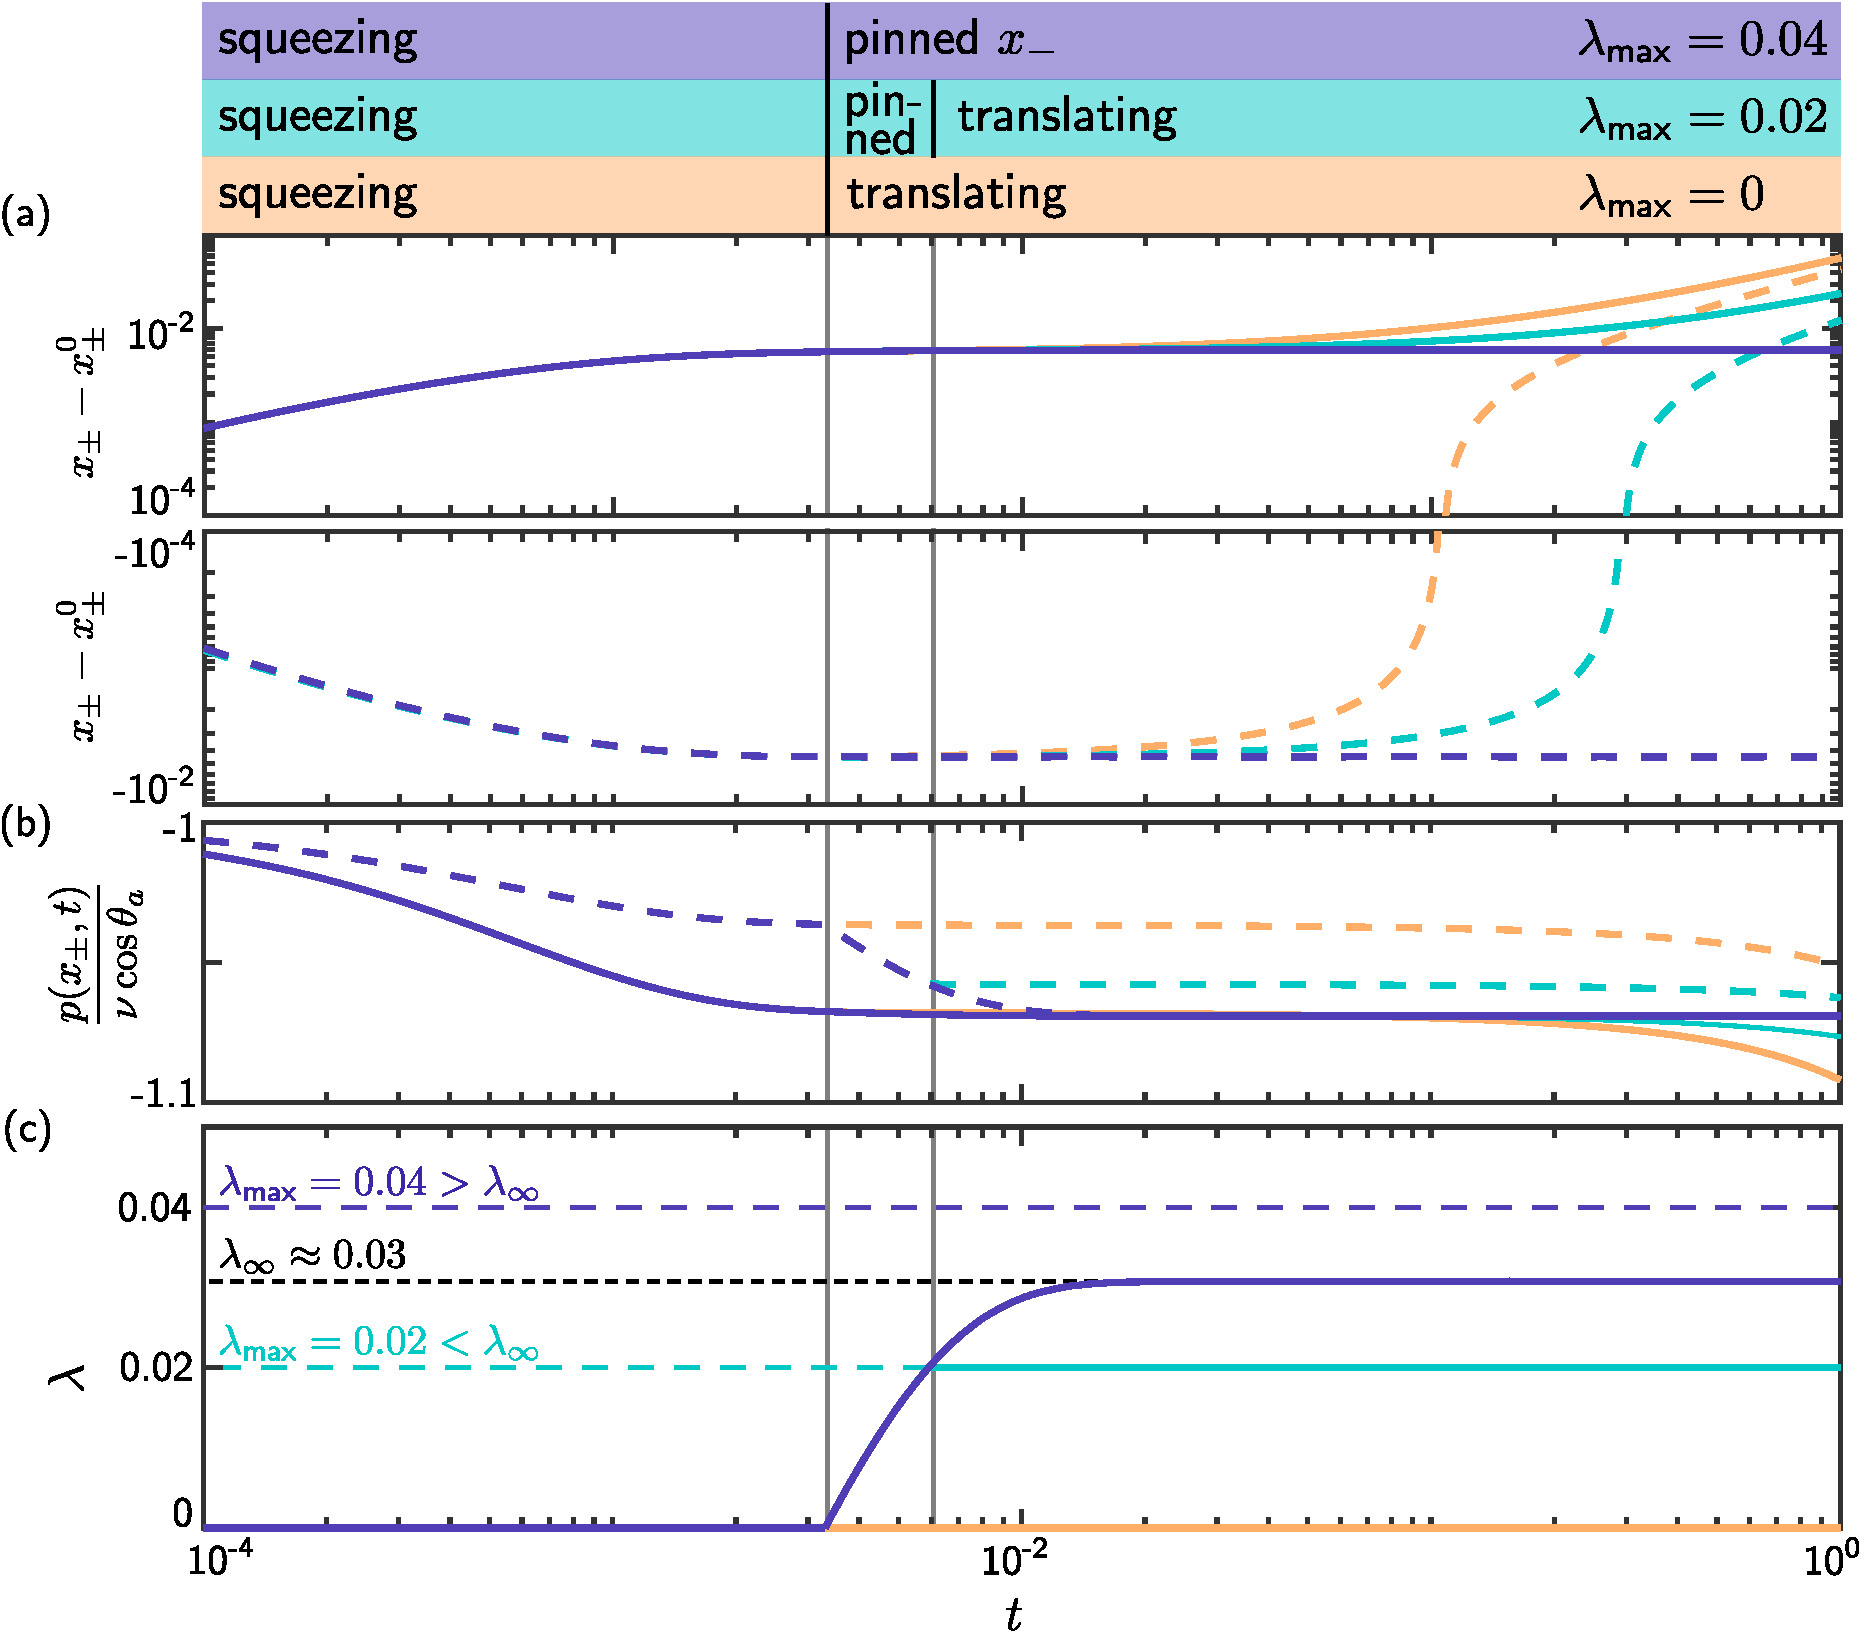
\includegraphics[width = 0.9\textwidth]{example_solutions_stacked_v3}
\caption{Numerical simulations of bendotaxis with contact angle hysteresis. The plots show (a) the displacement of the menisci away from their initial positions, (b) the normalized meniscus pressure, and (c) the contact angle asymmetry $\hyspar$.  In each plot, solid curves correspond to results for the `$+$' meniscus while dashed curves correspond to  results for the `$-$' meniscus. In each case, $\theta_r = 0\si{\degree}$, and solutions are shown for three different values of the contact angle hysteresis $\hyspar_{\text{max}}$ as follows: $\hyspar_{\text{max}} = 0$ (orange curves, i.e.~no contact angle hysteresis), $\hyspar_{\text{max}} = 0.02$ (green curves,  $\theta_a = 10\si{\degree}$ -- relatively small contact angle hysteresis), and $\hyspar_{\text{max}} = 0.04$ (purple curves, $\theta_a = 16\si{\degree}$ -- relatively large contact angle hysteresis). In each case, $\nu =  4, \xright^0 = 0.65, V = 0.2$ (i.e. $\xleft^0= 0.45$).  A log-log scale is used in (a) to aid distinction between the curves. The motion can be split into (at most) three temporal regions based on the direction of motion of the menisci; these are referred to as squeezing, pinned $\xleft$, and translating as indicated at the top of the figure. In (c), the coloured horizontal dashed lines indicate the corresponding value of $\hyspar = \hysparmax$ and the black dashed line indicates $\hyspar = \hyspar_{\infty}$ -- the contact angle asymmetry that the system would saturate at for $\hyspar_{\text{max}} \gg 1$ (see main text).}\label{fig:Ch4:Hysteresis:ExampleTraces}
\end{figure}


In this section, we consider numerical solutions of the system~\eqref{E:Ch4:Geometric:Model:flow_eq1}--\eqref{E:Ch4:Geometric:Model:flow_eq3} with the boundary conditions listed in Table~\ref{T:Ch4:Geometric:BoundaryConditions} and modified kinematic conditions~\eqref{E:ch4:Hysteresis:Parametrisation:kbc_and_laplace}--\eqref{E:ch4:Hysteresis:Parametrisation:ic_theta_wetting}. These numerical solutions offer insight into how hysteresis affects the dynamics of bendotaxis, showing how the various transitions between boundary conditions described in \S\ref{S:Ch4:hysteresis:modelling} might occur in practice, and offer insight into one route by which droplets may be trapped within a channel.

\subsubsection{Modifications to numerical scheme}
It is straightforward to modify the numerical scheme described in \S2.2 and \S4.1.2 to include contact angles that evolve dynamically within this model of hysteresis. Transitions between advancing, pinned, and receding conditions at each meniscus are determined by evaluating appropriate event-detection functions at each time-step, as outlined in the flowchart in Figure~\ref{fig:Ch4:Hysteresis:Flowchart}. Note that several of the nine possible (three at each meniscus) combinations of states (advancing, pinned or receding) for $(\theta_+, \theta_-)$ are not realizable as they would require a violation of conservation of mass; for example, receding angles at both menisci, $\theta_+ = \theta_r, \theta_- = \theta_r$, is incompatible with wetting conditions in which the channel walls are deflected inwards.

Note that here we consider only channels in regime I (open ends), although our numerical scheme is capable of describing any combination of the boundary conditions at $x = x_{\pm}$ and $x = 1$ that arise from the various contact angle and contacting conditions described in \S4.1 and \S\ref{S:Ch4:hysteresis:modelling}.

\subsubsection{Dynamics}
In Figure~\ref{fig:Ch4:Hysteresis:ExampleTraces}, we show numerically obtained traces of the displacement of the menisci, the normalized meniscus pressure, and contact angle asymmetry for three different values the advancing contact angle as follows: $\theta_a = 0\si{\degree}$,  $\theta_a = 10\si{\degree}$, and $ \theta_a =16\si{\degree}$, all with $\theta_r = 0\si{\degree}$. The corresponding values of the contact angle hysteresis $\hysparmax$ are $\hysparmax = 0$, $\hysparmax = 0.02$, and $\hysparmax = 0.04$, respectively. (These correspond to systems with no contact angle hysteresis, relatively small contact angle hysteresis and relatively large contact angle hysteresis, respectively, as we shall see.)

\paragraph{Initial behaviour.}
The three solutions have identical initial conditions ($\xright^0 = 0.65, \xleft^0 =0.45$), and are thus identical at early times (the droplet does not have any information about the maximum possible contact angle asymmetry, $\hyspar_{\text{max}}$, while $\hyspar < \hyspar_{\text{max}}$). In this squeezing period, the droplet has the advancing contact angle at both menisci, so $\hyspar = 0$ (Figure~\ref{fig:Ch4:Hysteresis:ExampleTraces}(c)) and the behaviour is identical to the early time behaviour described in Chapter 2 -- the droplet responds to the initial torque imbalance and the pressure decreases with time at both menisci as the confinement becomes stronger (Figure~\ref{fig:Ch4:Hysteresis:ExampleTraces}(b)).

\paragraph{Pinning of $\xleft$.}
As the channel continues to deform inwards, the pressure gradient at $\xleft$ decreases, eventually reaching zero so that this meniscus becomes pinned -- the advancing boundary condition~\eqref{E:ch4:Hysteresis:Parametrisation:BC_xleft}a is replaced by the pinned boundary condition~\eqref{E:ch4:Hysteresis:Parametrisation:BC_xleft}b. We refer to the subsequent time period as `pinned $\xleft$' to reflect this change in boundary conditions (see Figure~\ref{fig:Ch4:Hysteresis:ExampleTraces}).

The behaviour of the solutions for different values of $\hyspar_{\text{max}}$ diverges at this point: if $\hyspar_{\text{max}} = 0$, the pinned meniscus  immediately unpins (since $\theta_a = \theta_r = 0\si{\degree}$ throughout). The meniscus $\xleft$ turns and moves towards the free end (orange traces in Figure~\ref{fig:Ch4:Hysteresis:ExampleTraces}); these dynamics are precisely those discussed in Chapter 2.

For $\hyspar_{\text{max}} > 0$, $\xleft$ remains pinned for a  period of time.  $\xright$ continues to advance and the channel deformation continues to increase, thus reducing the pressure at $\xright$ (increasing the suction) and maintaining $\theta_+ = \theta_a$. To maintain a pinned condition at $\xleft$, the contact angle difference $\hyspar$  increases (the contact angle $\theta_-$ decreases, increasing $\cos \theta_-$, which acts to increase the magnitude of the suction pressure via the Laplace pressure condition~\eqref{E:ch4:Hysteresis:Parametrisation:kbc_and_laplace}). Independent of the value of $\hysparmax$, there is a limit to how much the channel can deform, and thus to how much the pressure can change, while $\xleft$ remains pinned. There is therefore a value of $\hyspar$, which we denote by $\hyspari$, at which the meniscus remains pinned indefinitely and reaches equilibrium. The value of $\hyspari$ depends on $\nu, V, \xright^0$ but emerges from the dynamic model -- it is not possible to determine it a priori, though our simulations suggest $\hyspari = 0.03$ for the values $\nu = 4, V = 0.2, \xright^0 = 0.65$ used here.

Whether the droplet leaves the pinned $\xleft$ stage depends on whether $\hyspar$ reaches $\hyspari$ without first reaching the maximum allowed contact angle asymmetry $\hysparmax$, at which point $\xleft$ must de-pin. If the contact angle hysteresis is relatively large then $\hysparmax > \hyspari$ (purple curves in Figure~\ref{fig:Ch4:Hysteresis:ExampleTraces}), so $\hyspar$ reaches $\hyspari$ first, and, when it does so, the droplet remains trapped partway along the channel with $\xleft$ pinned indefinitely. If the contact angle hysteresis is relatively small, then $\hysparmax \leq \hyspari$ (green curves in Figure~\ref{fig:Ch4:Hysteresis:ExampleTraces}), so $\hyspar$ reaches the maximum allowed asymmetry, $\hysparmax$, and the $\xleft$ contact line de-pins. We therefore have $\theta_- = \theta_r$ (recall that $\theta_+ = \theta_a$ still) and the droplet begins to translate to the free end of the channel. In summary, when contact angle hysteresis is small, the maximum contact angle asymmetry $\hysparmax$ is insufficient to maintain the pinned $\xleft$ state and the droplet translates to the free end via bendotaxis. If the maximum allowed asymmetry is sufficiently large, $\hysparmax > \hyspari$, then the droplet is trapped. (Note that as $\hysparmax \to \infty$, the contact angle asymmetry will always saturate at $\hyspar = \hyspari$.)

%if we reach the third period, droplet escapes. A point to make is that this sequential behaviour is generic (i.e. wetting droplets always do period 1 -> period 2 OR period 1-> period 2 -> period 3, and we only see at most three of the possible 9 combinations of boundary conditions).


\subsubsection{Discussion of dynamics}
These numerical solutions highlight two important points: firstly, they demonstrate that even a moderate amount of hysteresis can have a significant influence on the dynamics of bendotaxis; in the  simulation with relatively small contact angle hysteresis ($\theta_a =  10\si{\degree}$, $\theta_r =  0\si{\degree}$) the droplet takes approximately twice as long to reach the free end as the case of no hysteresis ($\theta_a =  \theta_r =  0\si{\degree}$). (This sensitivity of the dynamics to contact angle hysteresis justifies the care taken to minimize it in the experimental study of bendotaxis presented in Chapter 3.)

Secondly, these simulations confirm our intuition that when hysteresis is sufficiently strong, droplets may get trapped part way along the channel. The numerical solutions highlight three important features of the trapping mechanism, that appear to be generic:
firstly, the system always passes through a squeezing period, after $\xleft$ is pinned; secondly there is a contact angle asymmetry, $\hyspari$, required to maintain the pinned conditions indefinitely; and, thirdly, if $\hysparmax \leq \hyspari$, the maximum contact angle asymmetry is not enough to pin the droplet and it begins to translate, but if $\hysparmax > \hyspari$ the droplet remains in the pinned state.

\subsubsection{Effect of droplet initial position}
\begin{figure}[t]
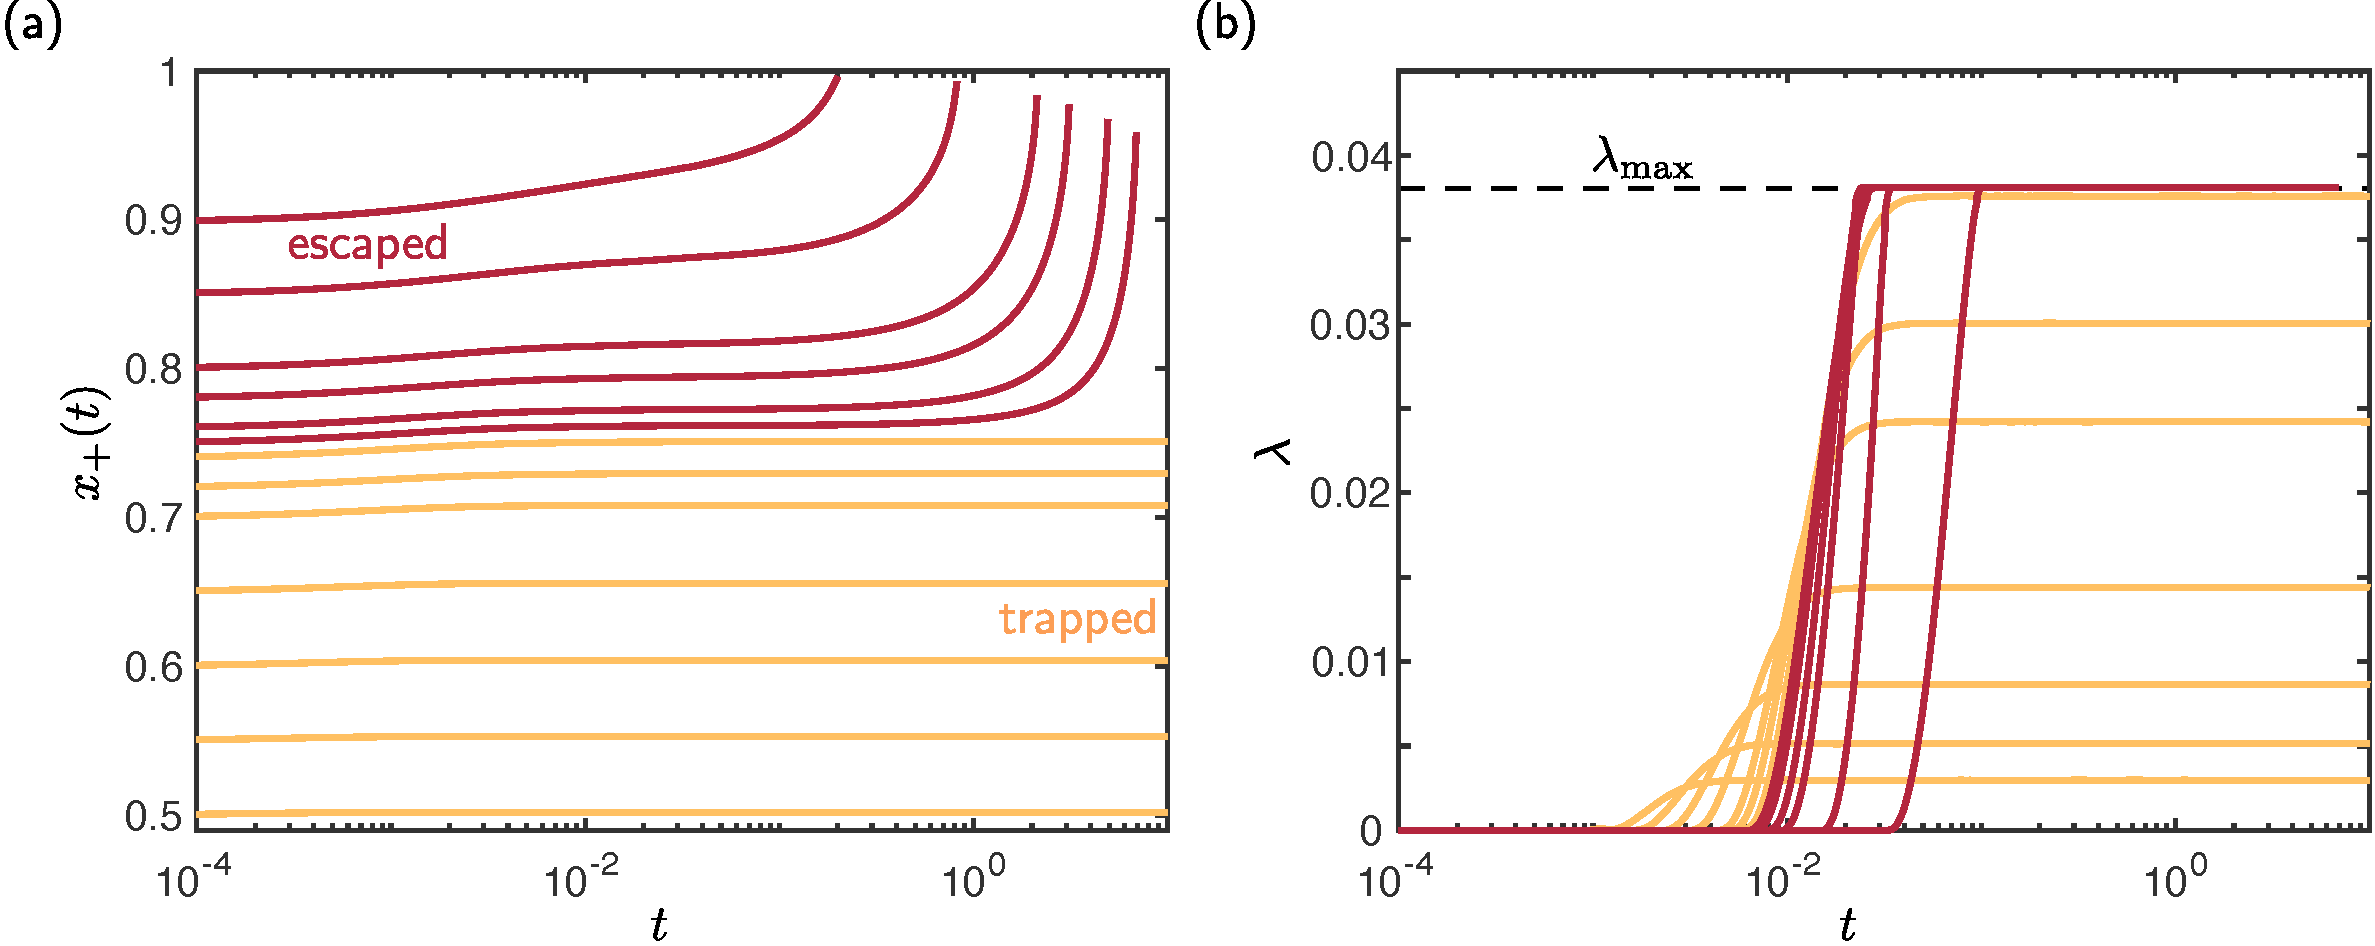
\includegraphics[width = 0.95\textwidth]{escape_traces}
\caption{(a) Meniscus position $\xright(t)$ and (b) contact angle asymmetry $\hyspar$ in simulations of bendotaxis with contact angle hysteresis
for various initial meniscus positions in the range $0.5\leq \xright^0 \leq0.9$.  For each value of $\xright^0 = \xright(t = 0)$, $V = 0.2,~ \nu = 4,~ \hyspar_{\text{max}} = 0.038, ~\theta_r = 0\si{\degree}$ (corresponding to an advancing angle $\theta_a = 18\si{\degree}$). Note that droplets starting close to the free end ($\xright^0$ sufficiently large) escape, whilst those starting closer to the base are trapped indefinitely.}\label{fig:Ch4:Hysteresis:Numerics:initialpos}
\end{figure}

Further insight into the trapping mechanism can be gleaned by considering the effect of the initial position of the `$+$' meniscus, $\xright^0$. In Figure~\ref{fig:Ch4:Hysteresis:Numerics:initialpos}, we plot numerically obtained trajectories $\xright(t)$ and the corresponding evolution of the contact angle asymmetry $\lambda(t)$ for various initial conditions in the range $0.5 \leq \xright^0 \leq 0.9$. We see that for droplets that start close to the free end, $\hyspar$ reaches $\hysparmax$ so that the droplet begins to translate and ultimately reaches the free end (it `escapes'). However, for droplets that start closer to the base (smaller values of $\xright^0$), $\hyspar$ does not reach $\hysparmax$ before $\hyspari$ and the droplet remains trapped part way along the channel, close to its initial position. This behaviour suggests that $\hyspari$ is an increasing function of $\xright^0$, as we might expect -- a greater contact angle difference will be needed to maintain the pinned state when the droplet sits nearer the free end of the channel, which is easier to deform.

In the remainder of this chapter, we address the following question that is motivated by the dynamic numerical solutions just presented: when (i.e. in which regions of $(\nu, V, \xright^0, \hysparmax)$ space) do droplets get trapped as a result of contact angle hysteresis? The first step in approaching this question is to consider the configurations occupied when droplets are trapped, i.e. equilibria of the system, and so we turn to this now.
\subsection{Equilibrium configurations}\label{S:Ch4:Hysteresis:Equilibria}
The numerical solutions presented in \S\ref{S:Ch4:Hysteresis:Numerics} suggest that droplets can be trapped indefinitely if the contact angle hysteresis is sufficiently large (or equivalently that droplets start sufficiently close to the clamped end). In this section, we consider these trapped equilibrium states. We aim to determine when equilibria exist and analyse their linear stability, with a view to (i) verifying that the numerical solutions presented in \S\ref{S:Ch4:Hysteresis:Numerics} are indeed converging to true equilibria (rather than simply slowly evolving transients), (ii) checking that these equilibria are linearly stable and (iii) understanding whether it is ever possible for a droplet to become trapped after reaching the translating phase.

In this section, we consider equilibrium configurations for a general contact angle difference $\hyspar = \hyspare$; these results are then expected to be pertinent provided that $\hyspare$ is attainable, i.e. provided that $\hyspare \leq \hysparmax$.

\subsubsection{Equations for equilibrium}
%state the equations for equilibria, and an appendix describing how we solve them numerically (but mention key point that we don't actually specify V but rather xright). In particular, point out that the hysteresis condition can be thought of as a geometric constraint.
Equilibrium configurations can be recovered from the steady form of the dynamic problem (the PDE~\eqref{E:Ch4:Geometric:Model:flow_eq1}--\eqref{E:Ch4:Geometric:Model:flow_eq3} with the boundary conditions in Table~\ref{T:Ch4:Geometric:BoundaryConditions} but with the Laplace pressure condition replaced by~\eqref{E:ch4:Hysteresis:Parametrisation:kbc_and_laplace}b). Here we consider configurations in regime I, II or III, for completeness, but we are primarily interested in regime I because droplets in channels in regime II or III are already trapped (albeit via a different mechanism). As we shall see, only regime I equilibria exist in the region of parameter space of interest.

The problem for the equilibrium channel wall shape $h_e(x)$ with menisci located at $x_{\pm} = \xpmeq$ (as well as possibly for the contact point $x_c =\xceq$) is
\begin{align}
\dd{^4 h_e}{x^4} &= 0, & &\text{for}~ 0 < x < \xlefteq,\label{E:Ch4:Hyseresis:Equilibria:Eqs:Beam1}\\
\dd{^4 h_e}{x^4} &= p_0, & &\text{for}~ \xlefteq < x < \xrighteq,\label{E:Ch4:Hyseresis:Equilibria:Eqs:Beam2}\\
\dd{^4 h_e}{x^4} &= 0, & &\text{for}~ \xrighteq < x < 1,\label{E:Ch4:Hyseresis:Equilibria:Eqs:Beam3}
\end{align}
where $p_0$ is the equilibrium droplet pressure. $p_0$ is constant throughout the droplet (since we consider equilibrium) and so, in particular, the meniscus pressures equal $p_0$, i.e.
\begin{equation}\label{E:Ch4:Hyseresis:Equilibria:Eqs:BeamP}
p_0 = -\left.\frac{\nu}{h_e}\right|_{x = \xrighteq}  = -\left.\frac{\nu(1 + \hyspare) }{h_e}\right|_{x = \xlefteq}.
\end{equation}

The problem~\eqref{E:Ch4:Hyseresis:Equilibria:Eqs:Beam1}--\eqref{E:Ch4:Hyseresis:Equilibria:Eqs:BeamP} must be solved subject to further boundary conditions
\begin{equation}\label{E:Ch4:Hyseresis:Equilibria:Eqs:ClampedBC}
h_{e} = 1,\quad  \dd{h_e}{x} = 0, \quad \text{at}~x = 0,
\end{equation}
continuity conditions
\begin{equation}\label{E:Ch4:Hyseresis:Equilibria:Eqs:Continuity}
\left[h_e\right]_{\xpmeq^-}^{\xpmeq^+} = \left[\dd{h_e}{x}\right]_{\xpmeq^-}^{\xpmeq^+} = \left[\dd{^2 h_e}{x^2}\right]_{\xpmeq^-}^{\xpmeq^+}=\left[\dd{^3 h_e}{x^3}\right]_{\xpmeq^-}^{\xpmeq^+}  =0,
\end{equation}
and boundary conditions at the non-clamped end, which depend on the regime as:
\begin{align}
\left.\dd{^2 h_e}{x^2}\right|_{x = 1}  = \left.\dd{^3 h_e}{x^3}\right|_{x = 1} &= 0   & &\text{regime I (open ends),}\label{E:Ch4:Hyseresis:Equilibria:Eqs:FarEndBCFree}\\
\left.h_e\right|_{x = 1}  =   \left.\dd{^2 h_e}{x^2}\right|_{x = 1}&= 0  & &\text{regime II (touching ends),}\label{E:Ch4:Hyseresis:Equilibria:Eqs:FarEndBCTouching}\\
h_e(\xceq \leq x \leq 1) = \left.\dd{h_e}{x}\right|_{x = \xceq} =   \left.\dd{^2 h_e}{x^2}\right|_{x =\xceq} &= 0    & &\text{regime III (sticking ends).}\label{E:Ch4:Hyseresis:Equilibria:Eqs:FarEndBCSticking}
\end{align}
The solution $h_e(x)$ must also satisfy the global volume constraint,
\begin{equation}\label{E:Ch4:Hyseresis:Equilibria:Eqs:Volume}
V = \int_{\xlefteq}^{\xrighteq}h_e(x)~\mathrm{d}x.
\end{equation}

For any candidate equilibrium, we must also ensure that
\begin{align}
&h_e(1) > 0 & &\textsf{for regime I,}\label{E:Ch4:Hyseresis:Equilibria:Eqs:regimeI_constraint}\\
&\left.\dd{^3 h_e}{x^3}\right|_{x = 1} >0, \quad \left.\dd{h_e}{x}\right|_{x =1} <0 & &\textsf{for regime II,}\label{E:Ch4:Hyseresis:Equilibria:Eqs:regimeII_constraint}\\
&\xrighteq < \xceq < 1 & &\textsf{for regime III,}\label{E:Ch4:Hyseresis:Equilibria:Eqs:regimeIII_constraint}
\end{align}
as discussed in \S\ref{S:Ch4:Geometric:Model}.

Note that by re-arranging~\eqref{E:Ch4:Hyseresis:Equilibria:Eqs:BeamP}, the contact angle asymmetry $\hyspare$ can be expressed as a geometric constraint on the solution:
\begin{equation}\label{E:Ch4:Hyseresis:Equilibria:Eqs:hyspar_geometry}
\hyspare = \frac{h_e(\xlefteq)}{h_e(\xrighteq)} - 1.
\end{equation}

\subsubsection{Equilibria with $\xlefteq = 0$}
The equations for equilibrium~\eqref{E:Ch4:Hyseresis:Equilibria:Eqs:Beam1}--\eqref{E:Ch4:Hyseresis:Equilibria:Eqs:Volume} do not have an analytic solution in general. However, analytic progress can be made if we impose (instead of solving for) $\xlefteq = 0$. Although this is case is hypothetical (we do not expect the Laplace pressure boundary condition to hold when the liquid contacts the base, for example), it serves as a limiting case and will be useful in what follows.

In this case, the combination of the pressure condition~\eqref{E:Ch4:Hyseresis:Equilibria:Eqs:BeamP} and the clamped boundary condition~\eqref{E:Ch4:Hyseresis:Equilibria:Eqs:ClampedBC} mean that equilibrium pressure is simply $p_0 = \nu (1 + \hyspare)$, and we can find  analytic solutions with channel shapes
\begin{equation}\label{E:Ch4:Hyseresis:Equilibria:Eqs:analytic_sol}
h_e(x) = 1-\frac{\nu(\hyspare +1)}{24}\times\begin{cases} (x-\xrighteq)^4 + 4\xrighteq^3(x-\xrighteq) + 3\xrighteq^4, & 0 < x < \xrighteq\\
\xrighteq^3 (4x-\xrighteq) & \xrighteq < x <1.
\end{cases}
\end{equation}
where the meniscus position $\xrighteq$ satisfies
\begin{equation}\label{E:Ch4:Hyseresis:Equilibria:Eqs:analytic_sol_meniscus_position}
\xrighteq^4 = \frac{8\hyspare}{\nu (1 + \hyspare)^2}.
\end{equation}
To satisfy the volume constraint~\eqref{E:Ch4:Hyseresis:Equilibria:Eqs:Volume} we require
\begin{equation}\label{E:Ch4:Hyseresis:Equilibria:Eqs:analytic_sol_volume}
\nu = \frac{8}{V^4}\frac{\hyspare}{(1+\hyspare)^2}\left(\frac{3\hyspare + 5}{5\hyspare + 5}\right)^4.
\end{equation}
Provided~\eqref{E:Ch4:Hyseresis:Equilibria:Eqs:analytic_sol_volume} holds, the open ends constraint~\eqref{E:Ch4:Hyseresis:Equilibria:Eqs:regimeI_constraint} is
\begin{equation}\label{E:Ch4:Hyseresis:Equilibria:Eqs:analytic_sol_open_ends}
V > \frac{4\hyspare(3\hyspare + 5)}{5(\hyspare+1)(4\hyspare + 3)}.
\end{equation}

\subsubsection{Regime Diagrams}
\begin{figure}[t]
\centering
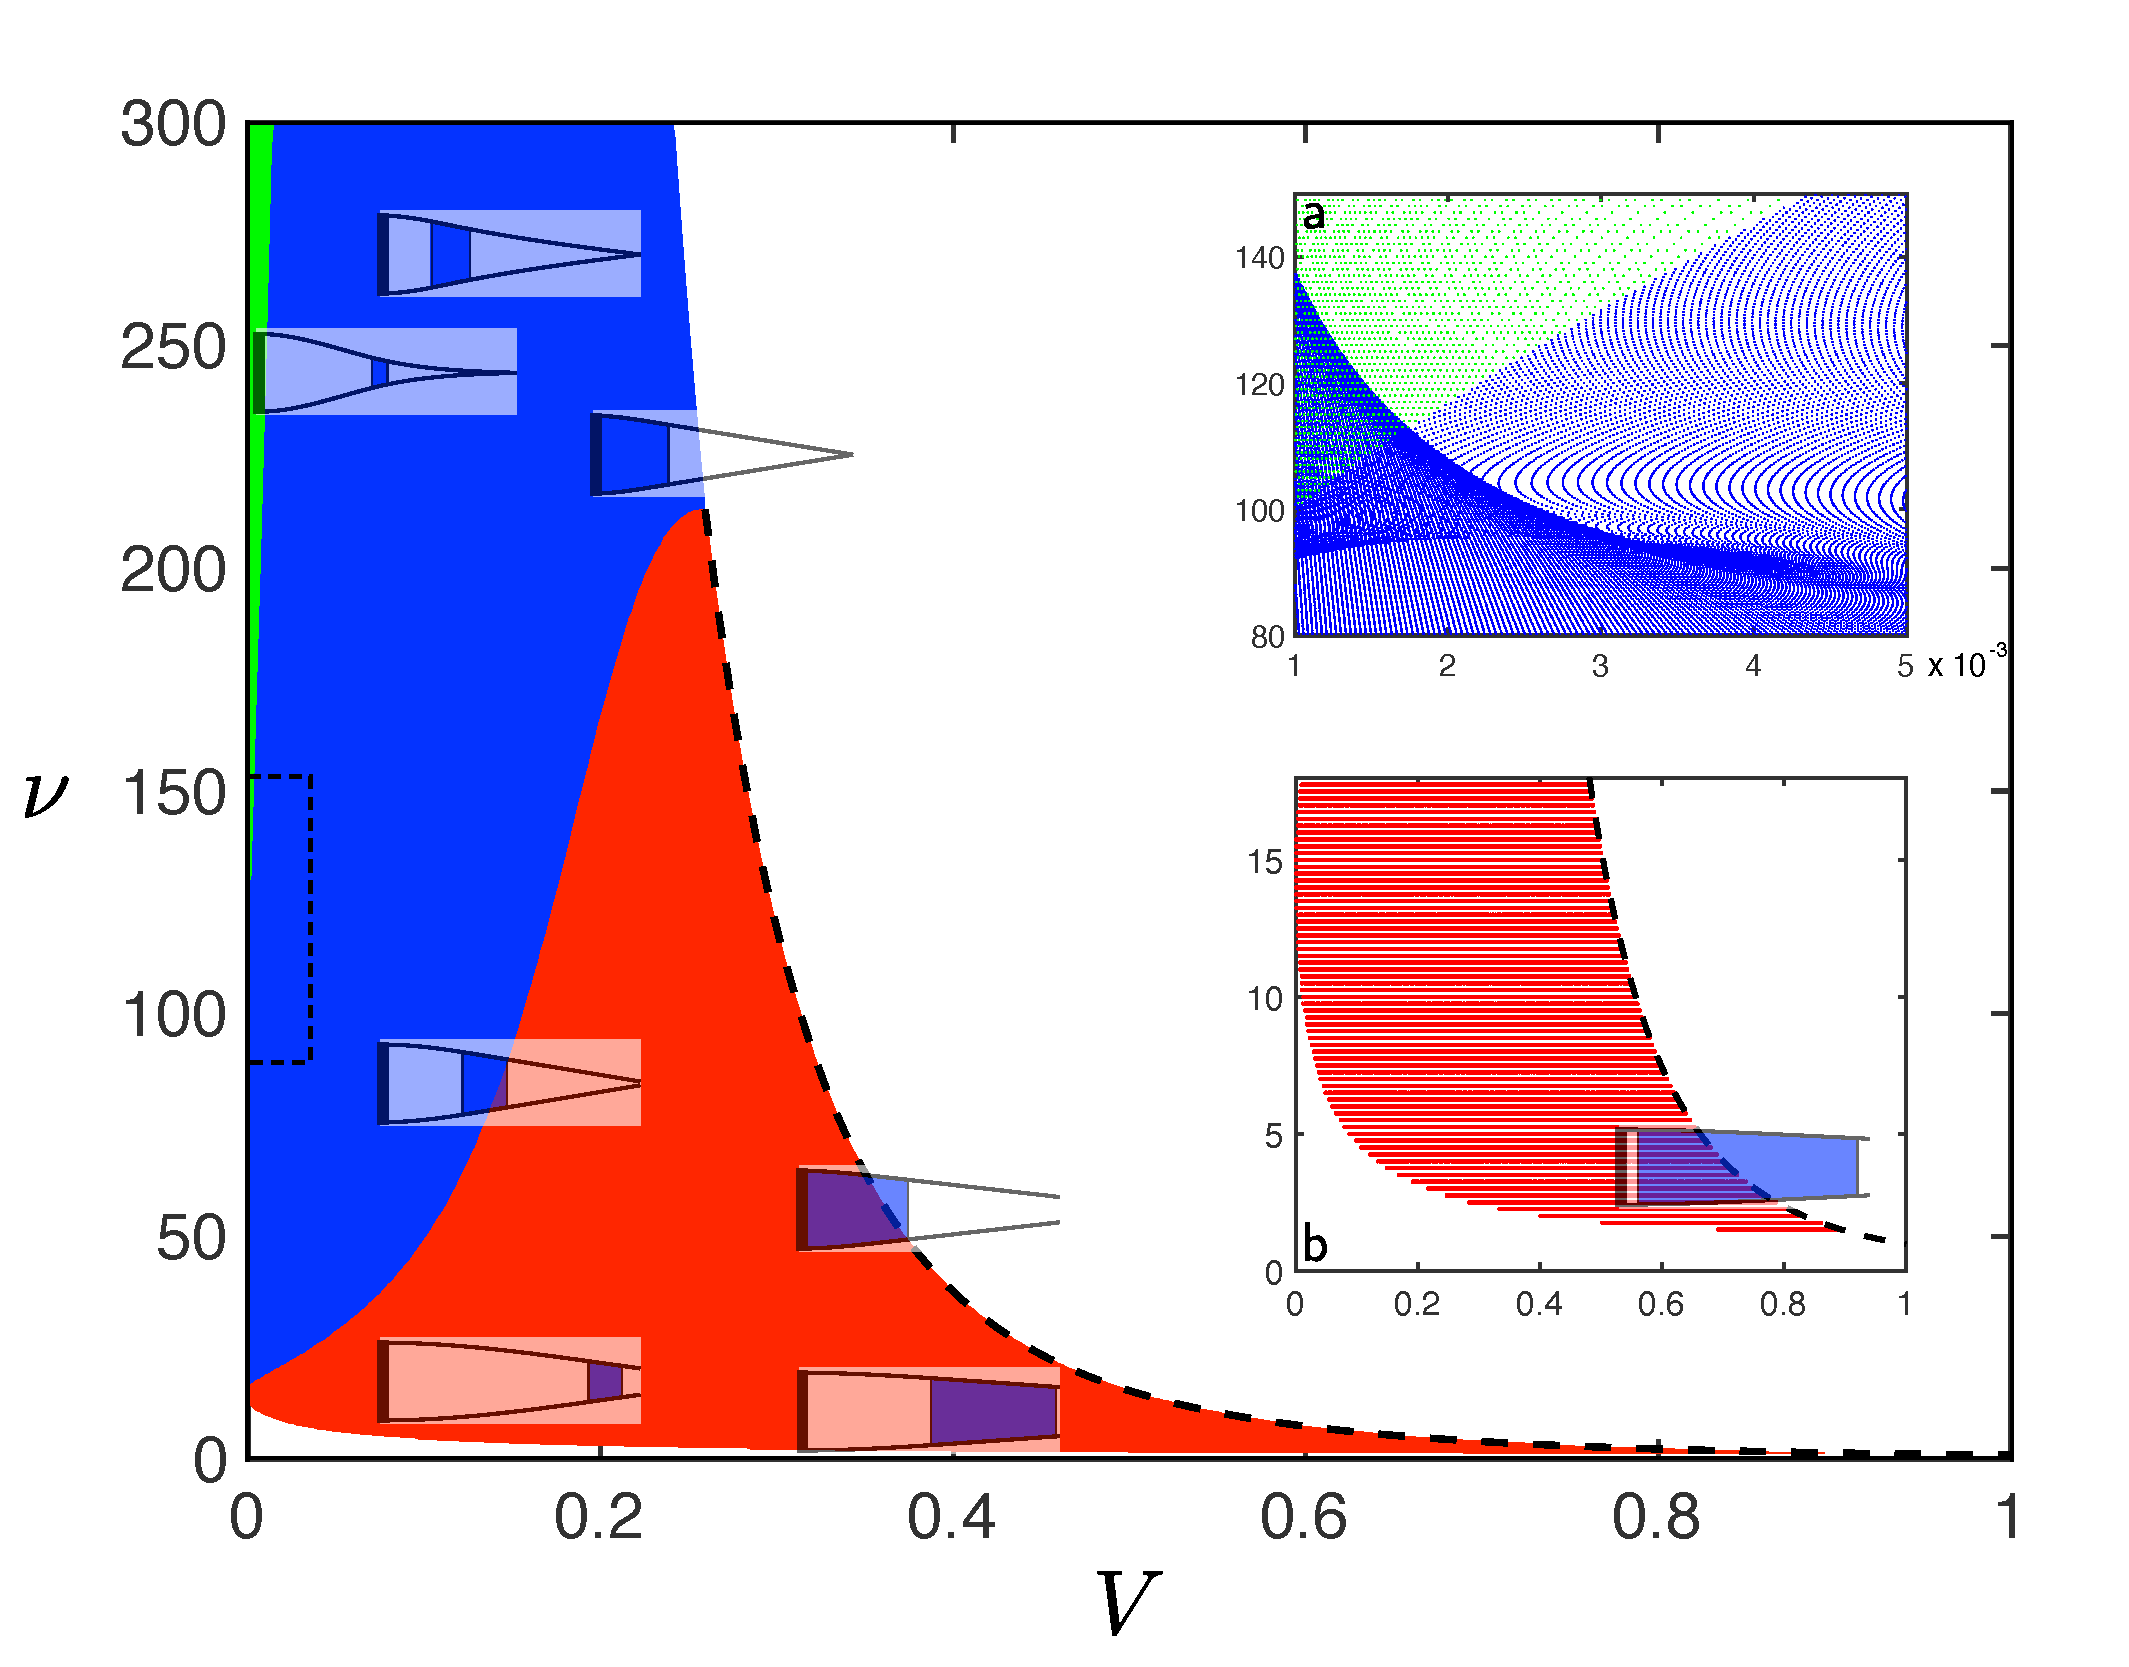
\includegraphics[width = 0.98\textwidth]{detailed_regime_diagram}
\caption{Regime diagram showing regions of $(V, \nu)$ space for which solutions of equations~\eqref{E:Ch4:Hyseresis:Equilibria:Eqs:Beam1}--\eqref{E:Ch4:Hyseresis:Equilibria:Eqs:Volume}  exist with $\hyspare = 0.3$. The schematic diagrams indicate the shape of the configuration close to that region of parameter space. The black dashed curve indicates~\eqref{E:Ch4:Hyseresis:Equilibria:Eqs:analytic_sol_volume}, corresponding to regime I equilibria with $X_- = 0$. Insets are close-ups of the main figure at (a) the dashed box, where multiple solutions exist with the same $(\nu, V)$ values, and (b) the region $0 < \nu < 17$, $0<V<1$. Points corresponding to regimes I, II and III are plotted as red, blue and green points, respectively. }\label{fig:Ch4:Hysteresis:ExampleRegimeDiagram}
\end{figure}

Equilibrium configurations are obtained numerically. Full details can be found in Appendix~\ref{A:Ch4:FindingEquilibria}, but we note that, for convenience, we do not solve the (non-linear) equilibrium equations~\eqref{E:Ch4:Hyseresis:Equilibria:Eqs:Beam1}--\eqref{E:Ch4:Hyseresis:Equilibria:Eqs:Volume} for given $(\nu, V, \hyspare)$ directly; rather we specify one of the meniscus positions (typically $\xlefteq$), and then solve the equations. The volume associated with each equilibrium is then readily calculated using~\eqref{E:Ch4:Hyseresis:Equilibria:Eqs:Volume}. By sweeping over all permissible values of $\xlefteq$, we pick up all possible solutions of~\eqref{E:Ch4:Hyseresis:Equilibria:Eqs:Beam1}--\eqref{E:Ch4:Hyseresis:Equilibria:Eqs:Volume}.

Equation~\eqref{E:Ch4:Hyseresis:Equilibria:Eqs:hyspar_geometry} encodes the fact that equilibria occur when the difference in contact angles $\hyspare$, exactly balances capillary induced wall deflections, whose size depends on the strength of surface tension (via $\nu$), the length over which the force is applied (via $V$) and the position of the droplet (via $\xrighteq$). In Figure~\ref{fig:Ch4:Hysteresis:ExampleRegimeDiagram} we show a regime diagram that indicates the regions of $(V, \nu)$ space in which equilibria exist. By presenting the data in this way, we address the question of how the droplet volume $V$ and bendability $\nu$ interact to create the required channel wall deflection. (Note that this example  with $\hyspare = 0.3$ corresponds to high contact angle asymmetry, but demonstrates the full range of possible behaviour; regime diagrams for smaller values of $\hyspare$ are shown in Figure~\ref{fig:Ch4:Hysteresis:RegimeDiagrams}.)

\begin{figure}[h!]
\centering
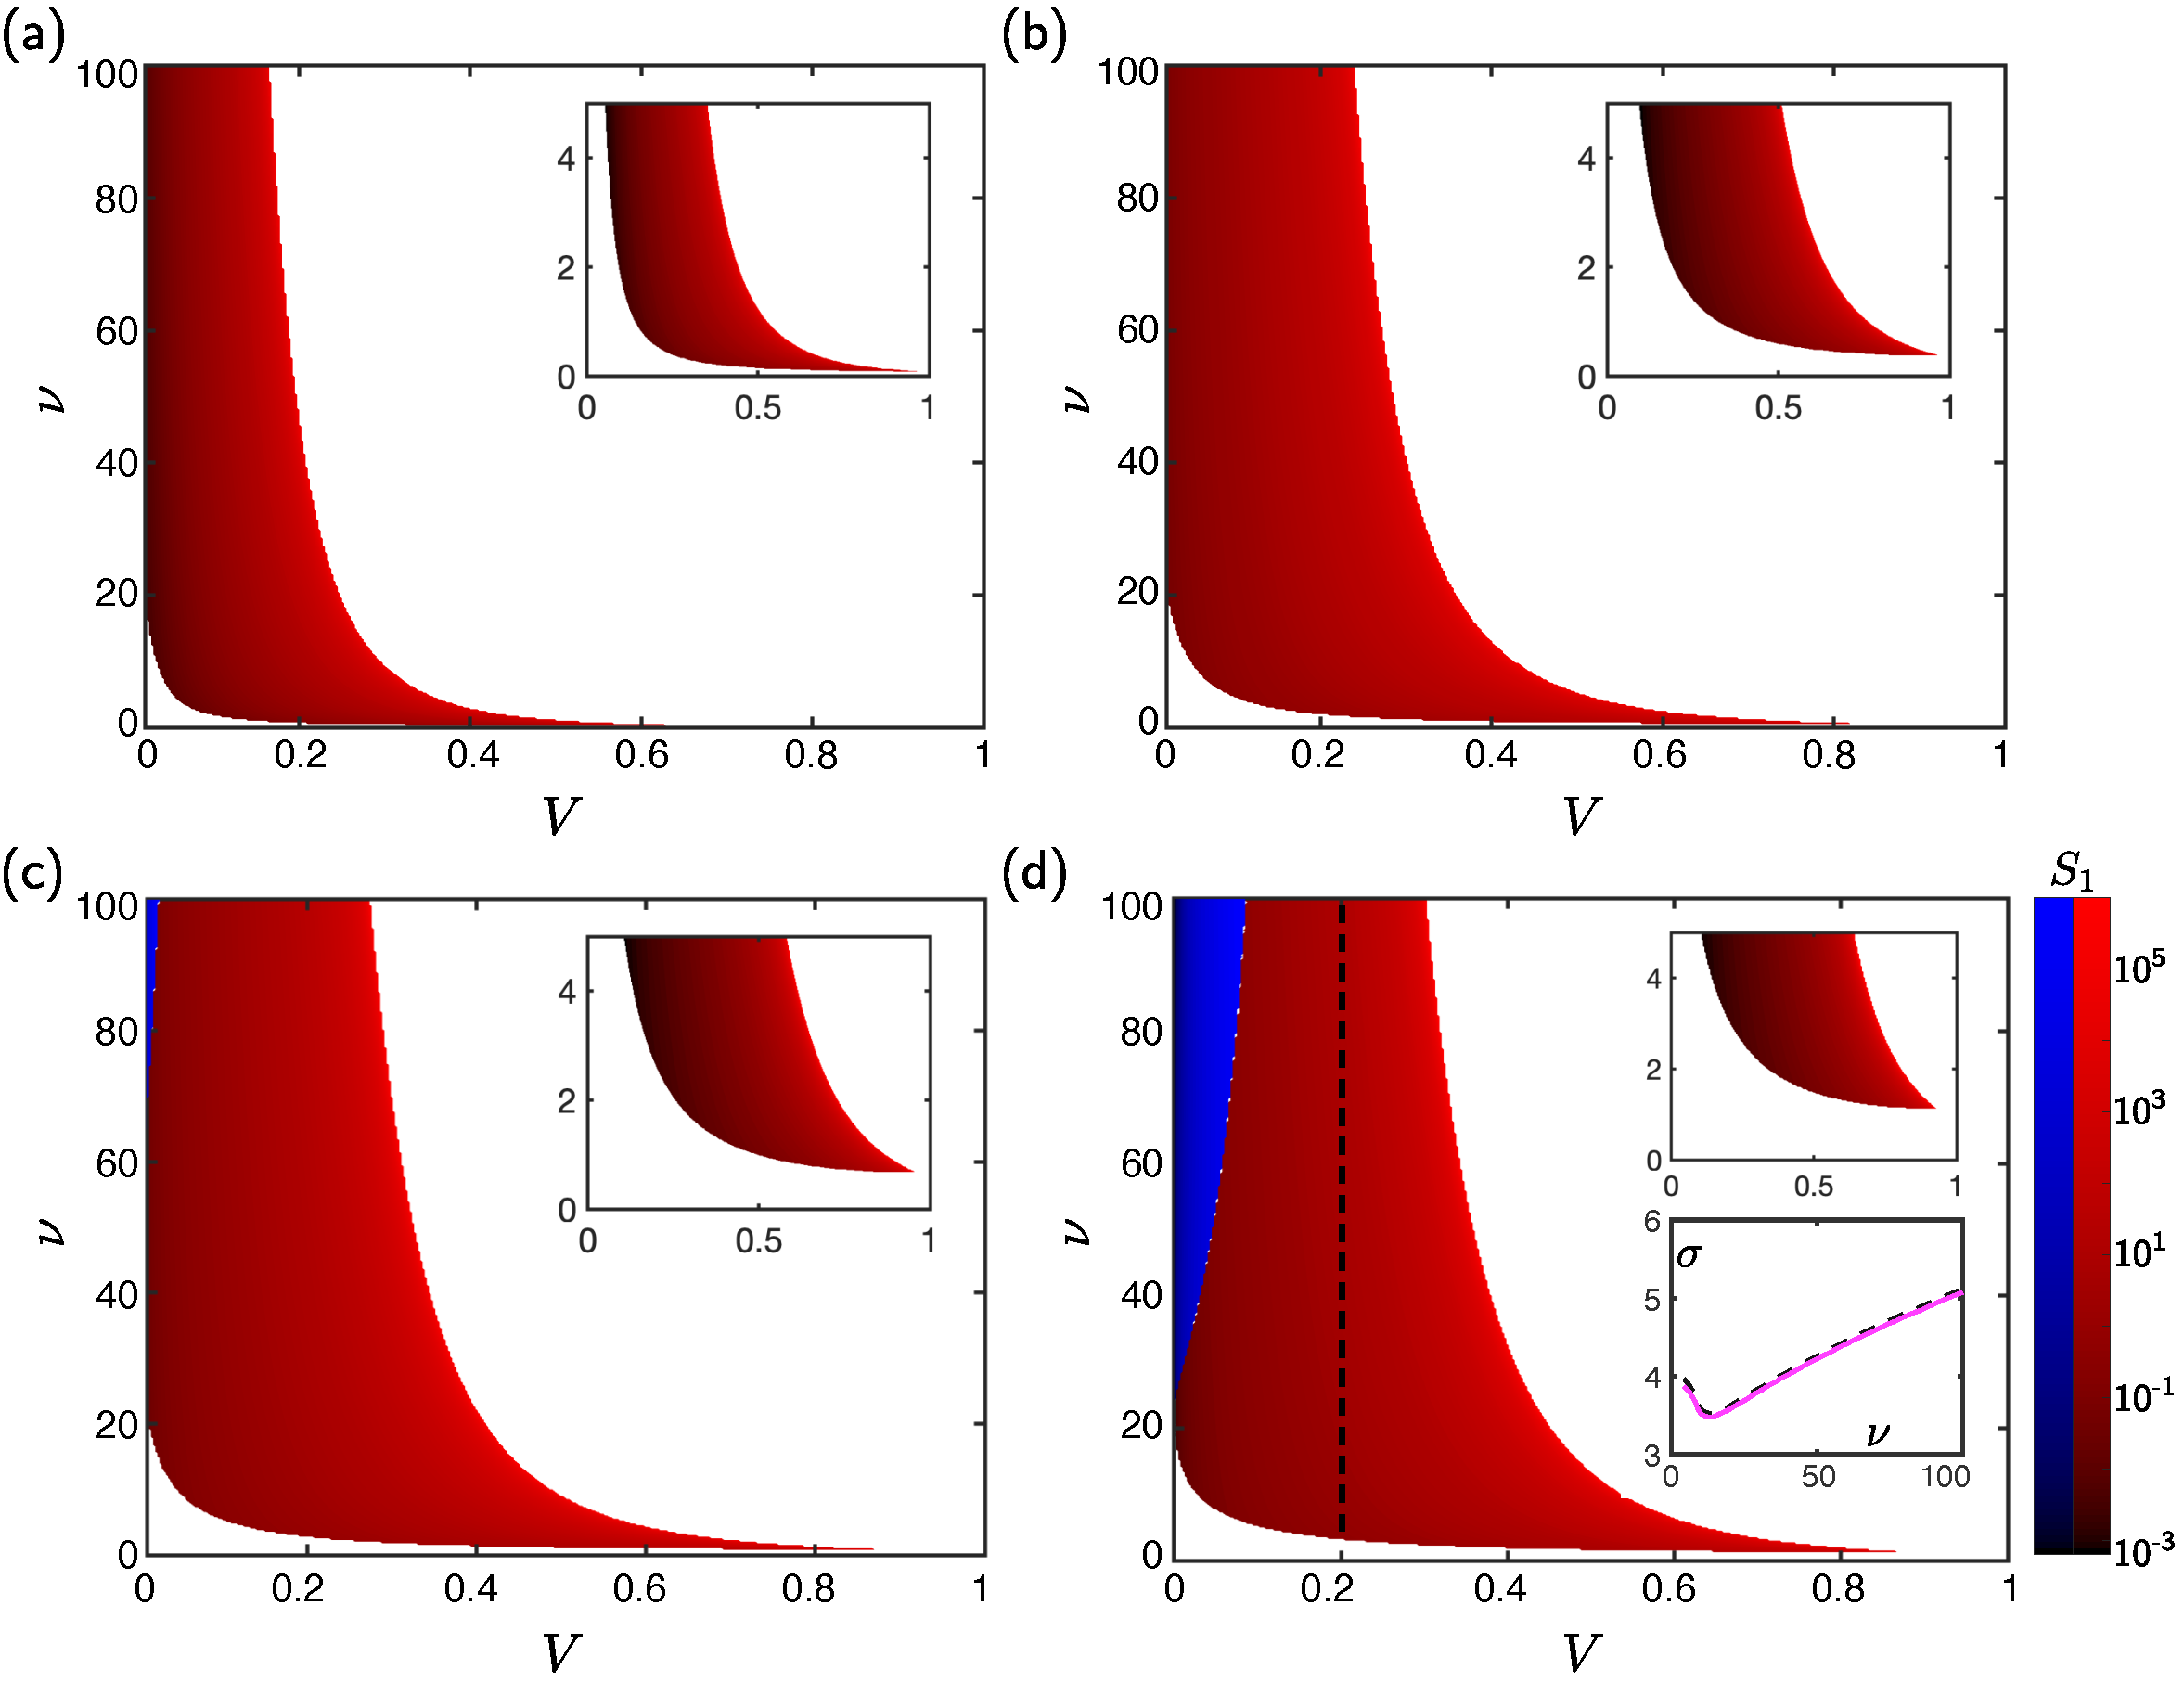
\includegraphics[width = 0.98\textwidth]{example_regime_diagrams}
\caption{Regime diagram showing regions of $(V, \nu)$ space for which solutions of equations~\eqref{E:Ch4:Hyseresis:Equilibria:Eqs:Beam1}--\eqref{E:Ch4:Hyseresis:Equilibria:Eqs:Volume}  exist for (a) $\hyspare = 0.01$, (b) $\hyspare = 0.05$, (c) $\hyspare = 0.1$, and (d) $\hyspare = 0.2$. The inset in each plot is as in the main plot, but zoomed into $0 < \nu < 5$. Red and blue regions indicate regime I  and II equilibria, respectively, and plot shading indicates the value of the constraint $S_1$ (defined in~\eqref{E:Ch4:Hyseresis:Equilibria:Stability:solvability}) according to the colour-bar in (d). The second inset in (d) indicates the growth rates $\sigma$ of perturbations to equilibria with $\hyspare = 0.2, V = 0.2$, as a function of $\nu$ (i.e. along the vertical dashed line in (d)) with the magenta curve corresponding to solutions of the BVP~\eqref{E:Ch4:Hyseresis:Equilibria:Stability:PDE1}--\eqref{E:Ch4:Hyseresis:Equilibria:Stability:kinematic} and the black dashed curve to numerical solutions of the (dynamic) model equations.}\label{fig:Ch4:Hysteresis:RegimeDiagrams}
\end{figure}

We can rationalize the shape of these regime diagrams by considering $\hyspare$ to be a geometric constraint on the capillary induced wall deflections. At small $\nu$ (weak surface tension), the Laplace pressure in the droplet is not able to create enough deflection to satisfy the geometric constraint~\eqref{E:Ch4:Hyseresis:Equilibria:Eqs:hyspar_geometry}, regardless of the droplet's size or position in the channel, and thus no equilibria exist. As $\nu$ increases, equilibria first appear with $\xrighteq = 1$ (see the schematics and inset b in Figure~\ref{fig:Ch4:Hysteresis:ExampleRegimeDiagram}),  since droplets are able to create the largest deflection when they are at the non-clamped end of the channel. This lower boundary of $\nu$ values is decreasing in $V$ (inset b) because larger droplets can generate the same deflection by applying a lower pressure (smaller $\nu$) over a larger area.

As $\nu$ increases (at the same volume $V$), equilibrium configurations have droplets closer to the base, where the higher bendability is countered by pressure being applied over relatively stiffer sections of channel. The channel width at the (currently free) end $x = 1$ is smaller in these equilibria.

Increasing $\nu$ further, regime I equilibria fail to exist when either (i) the channel width at the free end reaches zero, and regime II equilibria appear (blue region in Figure~\ref{fig:Ch4:Hysteresis:ExampleRegimeDiagram}), or, (ii) for larger volume droplets, the lower meniscus reaches the base ($\xlefteq = 0$) -- the droplet can move no further to offset increasing bendability (dashed line in Figure~\ref{fig:Ch4:Hysteresis:ExampleRegimeDiagram}, which corresponds to the analytic result~\eqref{E:Ch4:Hyseresis:Equilibria:Eqs:analytic_sol_volume}--\eqref{E:Ch4:Hyseresis:Equilibria:Eqs:analytic_sol_open_ends}). The boundary between regime II and regime III equilibria behaves in a qualitatively similar way, although it is located at much larger values of $\nu$.


Interestingly, there is a small region  of parameter space where $\nu \gg 1$ and $V \ll 1$ in which multiple equilibria exist (see inset~a in Figure~\ref{fig:Ch4:Hysteresis:ExampleRegimeDiagram}), but elsewhere at most one equilibrium exists. For a general $\hyspare$, the region where multiple equilibria exist is always on the border between regime II and III configurations, and with $V \ll 1$;  because of their small volume, however, these equilibria are considered to be a curiosity (and not physically relevant).

%key points: (i) we have to go to very large nu to get regime II, and regime III is basically non-existant (again can be understood in terms of the geometric constraint), (ii) there is a region of multiple solutions but it's very small (the difference with TV12 is the difference in boundary conditions).

%regime diagrams for different nu, V values.
Regime diagrams for smaller values of the contact angle difference $\hyspar_e$ are shown in Figure~\ref{fig:Ch4:Hysteresis:RegimeDiagrams}. We see that the minimum value of $\nu$ (for a fixed $V$) at which equilibrium configurations exist is smaller for smaller $\hyspar_e$ -- less deflection is needed to satisfy the geometric constraint~\eqref{E:Ch4:Hyseresis:Equilibria:Eqs:hyspar_geometry}, which can therefore be achieved with a lower surface tension. Similarly, the largest value of $\nu$ at which equilibrium configurations exist is also smaller for lower $\hyspare$.  In addition, equilibria in regime II and III are less prevalent; since the border between regime I and II equilibria is well beyond the range of ($\mathcal{O}(1)$) $\nu$ values that are of interest, we shall therefore consider only regime I equilibria for the remainder of this chapter (note that regime III equilibria do exist for $\hyspar_e \leq 0.2$ -- i.e.~in the range of values used in Figure~\ref{fig:Ch4:Hysteresis:RegimeDiagrams} -- but they do not appear on the scale of the plot).

In Figure~\ref{fig:Ch4:Hysteresis:regime_diagrams_xright_and_hyspar_vs_nu} we show two other ways of describing where equilibria exist. Firstly, in Figure~\ref{fig:Ch4:Hysteresis:regime_diagrams_xright_and_hyspar_vs_nu}(a), we plot the value of $\hyspare$ associated with equilibria in $(\xrighteq, \nu)$ space (for the $\mathcal{O}(1)$ values of the bendability $\nu$ that we are interested in). This plot indicates that equilibria in which the droplet is located closer to the free end are associated with a larger $\hyspare$, encoding a larger difference between the channel widths at the menisci, and that this difference is more pronounced for larger $\nu$.

Secondly, in Figure~\ref{fig:Ch4:Hysteresis:regime_diagrams_xright_and_hyspar_vs_nu}(b), we plot the value of $\xrighteq$ associated with equilibria in $(\hyspare, \nu)$ space. In particular, this plot indicates that equilibria do not exist when the contact angle asymmetry $\lambda_e$ is too large (the droplet is not able to create enough deflection to satisfy~\eqref{E:Ch4:Hyseresis:Equilibria:Eqs:hyspar_geometry}, regardless of where it sits in the channel) or too small (the droplet always creates too much deflection, regardless of where it sits in the channel).

\begin{figure}[t]
\centering
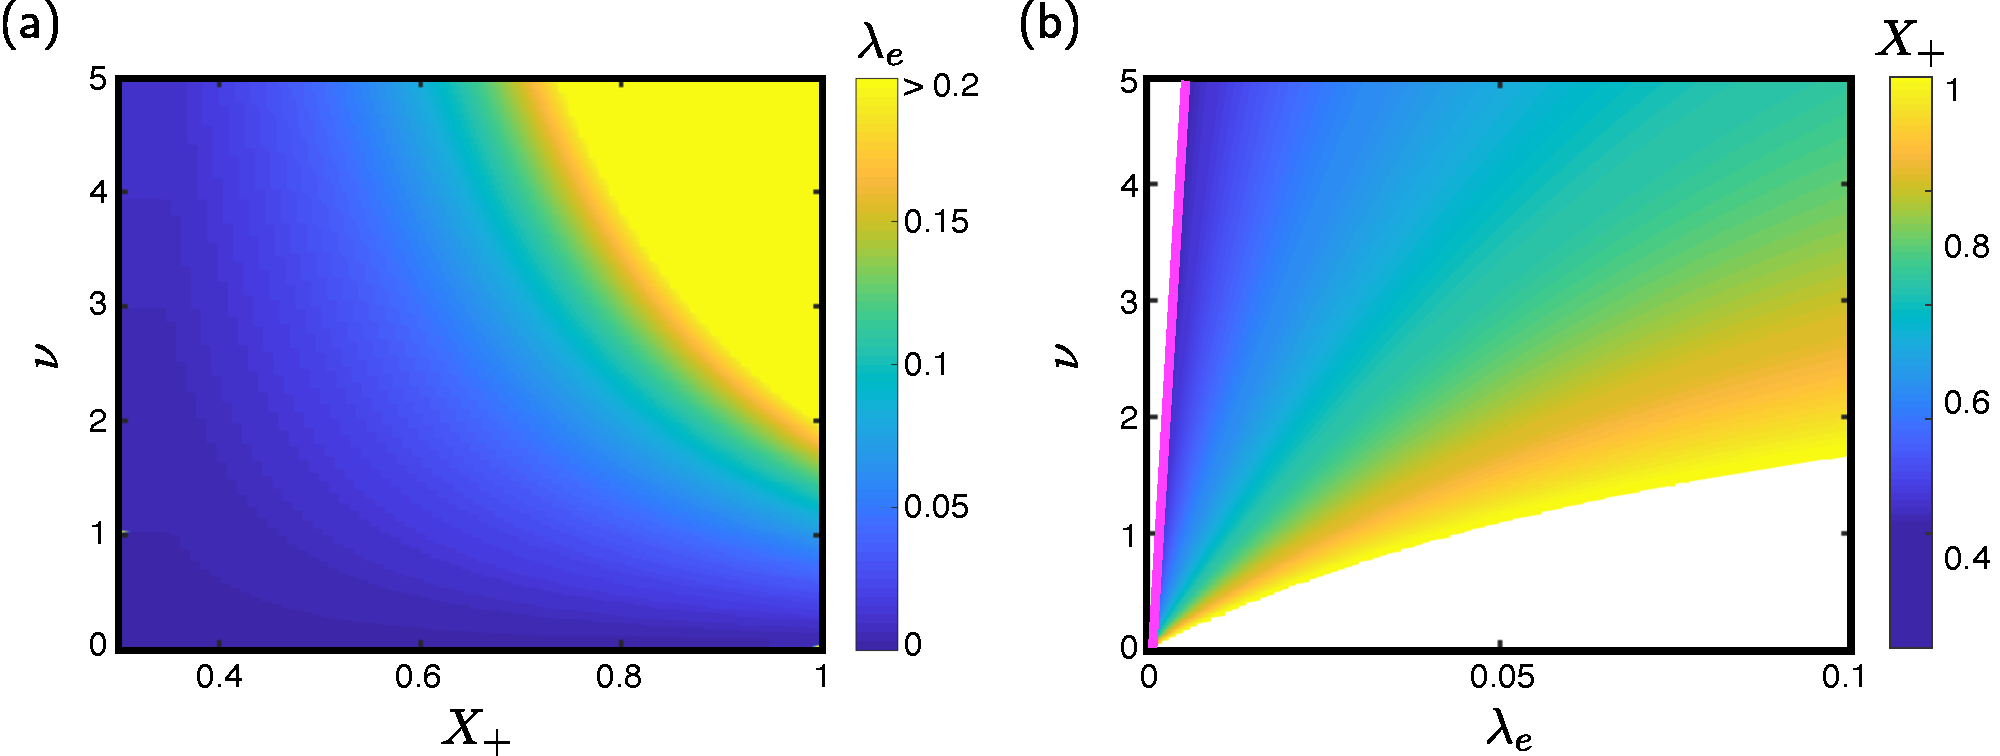
\includegraphics[width = 0.98\textwidth]{xright_and_hyspar_regime_diagram}
\caption{Regime diagrams indicating (a) the value of $\hyspare$ associated with equilibria in $(\xrighteq, \nu)$ space and (b) the value of $\xrighteq$ associated with equilibria in $(\hyspare, \nu)$ space (with $V = 0.3$ in both cases). In (b), no equilibria exist in the white region in the top left and bottom right corners, and the pink line indicates equilibria with $\xlefteq = 0$ (equation~\eqref{E:Ch4:Hyseresis:Equilibria:Eqs:analytic_sol_volume}).}\label{fig:Ch4:Hysteresis:regime_diagrams_xright_and_hyspar_vs_nu}
\end{figure}
\subsubsection{Stability}
We analyze the linear stability of equilibria by letting
\begin{equation}\label{E:Ch4:Hyseresis:Equilibria:Stability:perturbation}
h = h_e(x) + \epsilon e^{\sigma t} h_1(x), \qquad x_{\pm}(t) = \xpmeq +  \xpmeq^1  \epsilon e^{\sigma t} ,
\end{equation}
where $\epsilon \ll 1$ is arbitrary, in the model equations. For simplicity, we assume that the contact angles $\theta_{\pm}$  (and thus $\hyspar= \hyspar_e $), are unchanged by the perturbation (we use the boundary conditions on $h_1$ to reflect the contact angle conditions, see below).

After a standard linearization, the problem for $h_1(x)$ becomes
\begin{align}
0 &= \dd{^4 h_1}{x^4} & & 0 < x < \xlefteq,~\xrighteq < x < 1,\label{E:Ch4:Hyseresis:Equilibria:Stability:PDE1}\\
3|\nu|\sigma h_1 &=\dd{}{x} \left(h_e^3 \dd{^5 h_1}{x^5}\right) & &\xlefteq < x < \xrighteq,\label{E:Ch4:Hyseresis:Equilibria:Stability:PDE2}
\end{align}
with boundary conditions,
\begin{align}
h_1 & = \dd{h_1}{x} = 0 & &\text{at}~x = 0,\\
\dd{^2 h_1}{x^2} &=\dd{^3 h_1}{x^3} = 0 & &\text{at}~x = 1,
\end{align}
continuity conditions,
\begin{align}
\left[h_1 + \xpmeq^1\dd{h_e}{x}\right]_{\xpmeq^-}^{\xpmeq^+} = \left[\dd{h_1}{x} + \xpmeq^1\dd{^2 h_e}{x^2}\right]_{\xpmeq^-}^{\xpmeq^+} &=0, \\ \left[\dd{^2 h_1}{x^2 } +\xpmeq^1 \dd{^3 h_e}{x^3}\right]_{\xpmeq^-}^{\xpmeq^+} = \left[\dd{^3 h_1}{x} +\xpmeq^1 \dd{^4 h_e}{x^4}\right]_{\xpmeq^-}^{\xpmeq^+}  &= 0,
\end{align}
and conservation of volume
\begin{equation}\label{E:Ch4:Hyseresis:Equilibria:Stability:kinematic}
0 = \int_{\xlefteq}^{\xrighteq}h_1 ~\mathrm{d}x - \xrighteq^1 h_e(\xrighteq) + \xlefteq^1 h_e(\xlefteq)
\end{equation}
The final (pressure) boundary conditions on~\eqref{E:Ch4:Hyseresis:Equilibria:Stability:PDE1}--\eqref{E:Ch4:Hyseresis:Equilibria:Stability:PDE2} at $x = \xpmeq$ depend on the pinning conditions. Here we consider two cases. Firstly, mobile conditions,
\begin{align}
\dd{^4h_1}{x^4} &= \frac{\nu(1+ \hyspare)}{h_e^2} \left(\xlefteq^1\dd{h_e}{x} + h_1\right) & &\text{at}~x = \xlefteq,\label{E:Ch4:Hyseresis:Equilibria:Stability:translatingbc1}\\
\dd{^4 h_1}{x^4} &= \frac{\nu}{h_e^2} \left( \xrighteq^1\dd{h_e}{x} + h_1\right)& &\text{at}~x = \xrighteq,\label{E:Ch4:Hyseresis:Equilibria:Stability:translatingbc2}
\end{align}
which are the linearized form of the Laplace pressure boundary conditions~\eqref{E:ch4:Hysteresis:Parametrisation:kbc_and_laplace}b with $\theta_+ = \theta_a$ and $\theta_- = \theta_r$ (i.e. $\hyspare = \hysparmax$) and are thus appropriate for the translating period of the numerical solutions presented in \S\ref{S:Ch4:Hysteresis:Numerics}.

Secondly, we consider a pinned meniscus at $\xlefteq$ and an advancing meniscus at $\xrighteq$, so that
\begin{align}
\dd{^5 h_1}{x^5}&=0 & &\text{at}~x = \xlefteq,\label{E:Ch4:Hyseresis:Equilibria:Stability:pinnedbc1} \\
\dd{^4 h_1}{x^4} &= \frac{\nu}{h_e^2} \left(X_+^1 \dd{h_e}{x} + h_1\right)& &\text{at}~x = \xrighteq,\label{E:Ch4:Hyseresis:Equilibria:Stability:pinnedbc2}
\end{align}
we expect this latter case to be appropriate for the `pinned $\xleft$' period of the numerical solutions of \S\ref{S:Ch4:Hysteresis:Numerics}, where $\hyspar < \hyspar_{\text{max}}$ with $\theta_+ = \theta_a$.

The boundary value problem (BVP) given by~\eqref{E:Ch4:Hyseresis:Equilibria:Stability:PDE1}--\eqref{E:Ch4:Hyseresis:Equilibria:Stability:kinematic} alongside either~\eqref{E:Ch4:Hyseresis:Equilibria:Stability:translatingbc1}--\eqref{E:Ch4:Hyseresis:Equilibria:Stability:translatingbc2} or~\eqref{E:Ch4:Hyseresis:Equilibria:Stability:pinnedbc1}--\eqref{E:Ch4:Hyseresis:Equilibria:Stability:pinnedbc2} may be solved numerically using the \texttt{BVP4c} routine implemented in \textsc{matlab} (for example). This returns the growth rate $\sigma$ as part of the solution. Numerical solutions of the BVP agree well (see inset in Figure~\ref{fig:Ch4:Hysteresis:RegimeDiagrams}(d)) with numerical solutions of the full model equations, in which the growth rate is determined by an exponential fit to the meniscus trajectory at early times.

We do not dwell on solutions on the BVP, however, because we are primarily interested in the stability (the sign of $\sigma$) of equilibria, rather than the time scale of evolution to and from them (the magnitude of $\sigma$). It is instructive to consider instead the marginal stability problem given by~\eqref{E:Ch4:Hyseresis:Equilibria:Stability:PDE1}--\eqref{E:Ch4:Hyseresis:Equilibria:Stability:kinematic} and~\eqref{E:Ch4:Hyseresis:Equilibria:Stability:translatingbc1}--\eqref{E:Ch4:Hyseresis:Equilibria:Stability:translatingbc2} or~\eqref{E:Ch4:Hyseresis:Equilibria:Stability:pinnedbc1}--\eqref{E:Ch4:Hyseresis:Equilibria:Stability:pinnedbc2}  with $\sigma = 0$. In this case~\eqref{E:Ch4:Hyseresis:Equilibria:Stability:PDE2} can be integrated directly to give
\begin{equation}\label{E:Ch4:Hyseresis:Equilibria:Stability:integrate_once}
h_e^3 \dd{^5 h_1}{x^5} = C
\end{equation}
where $C$ is a constant (equal to zero for pinned conditions, from~\eqref{E:Ch4:Hyseresis:Equilibria:Stability:pinnedbc1}). From~\eqref{E:Ch4:Hyseresis:Equilibria:Stability:integrate_once}, we can express $h_1$ in terms of $h_e$, and thus the conservation of volume equations~\eqref{E:Ch4:Hyseresis:Equilibria:Stability:kinematic} can be expressed as a non-linear constraint of the form
\begin{equation}\label{E:Ch4:Hyseresis:Equilibria:Stability:solvability}
S_i(\nu, V, \hyspare) = 0, \qquad i = 1,2.
\end{equation}
Here,  $i = 1$ corresponds to the translating boundary conditions~\eqref{E:Ch4:Hyseresis:Equilibria:Stability:translatingbc1}--\eqref{E:Ch4:Hyseresis:Equilibria:Stability:translatingbc2} and $ i = 2$ to the pinned boundary conditions~\eqref{E:Ch4:Hyseresis:Equilibria:Stability:pinnedbc1}--\eqref{E:Ch4:Hyseresis:Equilibria:Stability:pinnedbc2}.

Solutions to the marginal stability problem exist when~\eqref{E:Ch4:Hyseresis:Equilibria:Stability:solvability} holds. However, we find that $S_i> 0$ over the whole parameter space (the shading in Figure~\ref{fig:Ch4:Hysteresis:RegimeDiagrams} indicates the value of $S_1$), so that for either choice of boundary conditions, the growth rate $\sigma$ does not change sign ($\sigma$ is continuous).

For the translating boundary conditions~\eqref{E:Ch4:Hyseresis:Equilibria:Stability:translatingbc1}--\eqref{E:Ch4:Hyseresis:Equilibria:Stability:translatingbc2}, $\sigma > 0$ \textit{somewhere} in the domain (see inset in Figure~\ref{fig:Ch4:Hysteresis:RegimeDiagrams}(d)), and so $\sigma > 0$. For the pinned boundary conditions~\eqref{E:Ch4:Hyseresis:Equilibria:Stability:pinnedbc1}--\eqref{E:Ch4:Hyseresis:Equilibria:Stability:pinnedbc2}, the same reasoning gives $\sigma <0$ everywhere.

This demonstrates that if the system reaches an equilibrium in which $\xleft$ is pinned, that equilibrium is stable and the droplet remains trapped indefinitely. However, should the droplet reach the translating stage, it will not stop again as any equilibrium it reaches is unstable. (In any case, we do not expect the system to encounter any of these equilibria -- once the droplet has reached the translating stage, the contact angle asymmetry $\hyspar$ cannot increase further, so the pressure difference between the menisci will continue to grow since the channel deflection is enhanced when the droplet is closer to the free end.)

%?????
%need to add a note about our assumption of unchanged contact angles being appropriate for translating conditions, but we expect might  affect equilibria with $\hysparmax - \hyspare \ll 1$ when BC might change as a result of perturbation??


\subsection{Mobile Droplets}
We are now in a position to describe when droplets remain trapped part way along the channel as a result of contact angle hysteresis. We understand that droplets get trapped in stable equilibria  if they remain in the pinned $\xleft$ stage of the motion; this, in turn, is possible, when the maximum contact angle asymmetry, $\hysparmax$, is larger than $\hyspari$, the contact asymmetry required to maintain the pinned state indefinitely.  The crucial point to note is that if an equilibrium exists then the associated contact angle asymmetry $\hyspare(\nu, V, \xrighteq) \approx \hyspari(\nu, V, \xright^0 =\xrighteq)$: for a droplet with given volume $V$ in a channel with given bendability $\nu$, the contact angle asymmetry in equilibrium is approximately that for a pinned droplet with initial condition $\xright^0 = \xrighteq$. (Any difference between $\hyspare$ and $\hyspari$ is a result of the  meniscus motion in the squeezing period, which is brief, making the difference relatively small, see Figure~\ref{fig:Ch4:Hysteresis:ExampleTraces}). As an approximate criterion, therefore, we argue that droplets will be trapped in $\hysparmax \gtrsim \hyspare(\nu, V, \xrighteq = \xright^0)$, and will escape if $\hysparmax \lesssim\hyspare(\nu, V, \xrighteq = \xright^0)$.

With this approximate criterion, the regime diagrams in Figure~\ref{fig:Ch4:Hysteresis:regime_diagrams_xright_and_hyspar_vs_nu} can be re-purposed as maps describing whether droplets will be trapped or not, based on the value of $\hysparmax$ (these regime diagrams are shown again in Figure~\ref{fig:xright_and_hyspar_regime_diagrams} with updated labels to reflect this interpretation of the equilibria). Figure~\ref{fig:xright_and_hyspar_regime_diagrams}(a) therefore (approximately) indicates $\hysparmax^{\textsf{escape}}$, the largest value of $\hysparmax$ at which droplets with initial condition $\xright^0$ are still able to escape: droplets in channels with  $\hysparmax > \hysparmax^{\textsf{escape}}$ will remain trapped, but those in channels with $\hysparmax \leq \hysparmax^{\textsf{escape}}$ will escape. As we see from Figure~\ref{fig:xright_and_hyspar_regime_diagrams}(a) (and as we expected from the numerical solutions presented in \S\ref{S:Ch4:Hysteresis:Numerics}), $\hysparmax^{\text{escape}}$ is increasing in $\xright^0$, so that droplets starting closer to the free end are more likely to escape. We see that, in addition, for a large proportion of the initial droplet positions only a small amount of hysteresis is needed to ensure droplets are trapped ($\hysparmax^{\text{escape}} \ll 1$), again highlighting the sensitivity of our system to contact angle hysteresis.

\begin{figure}[t]
\centering
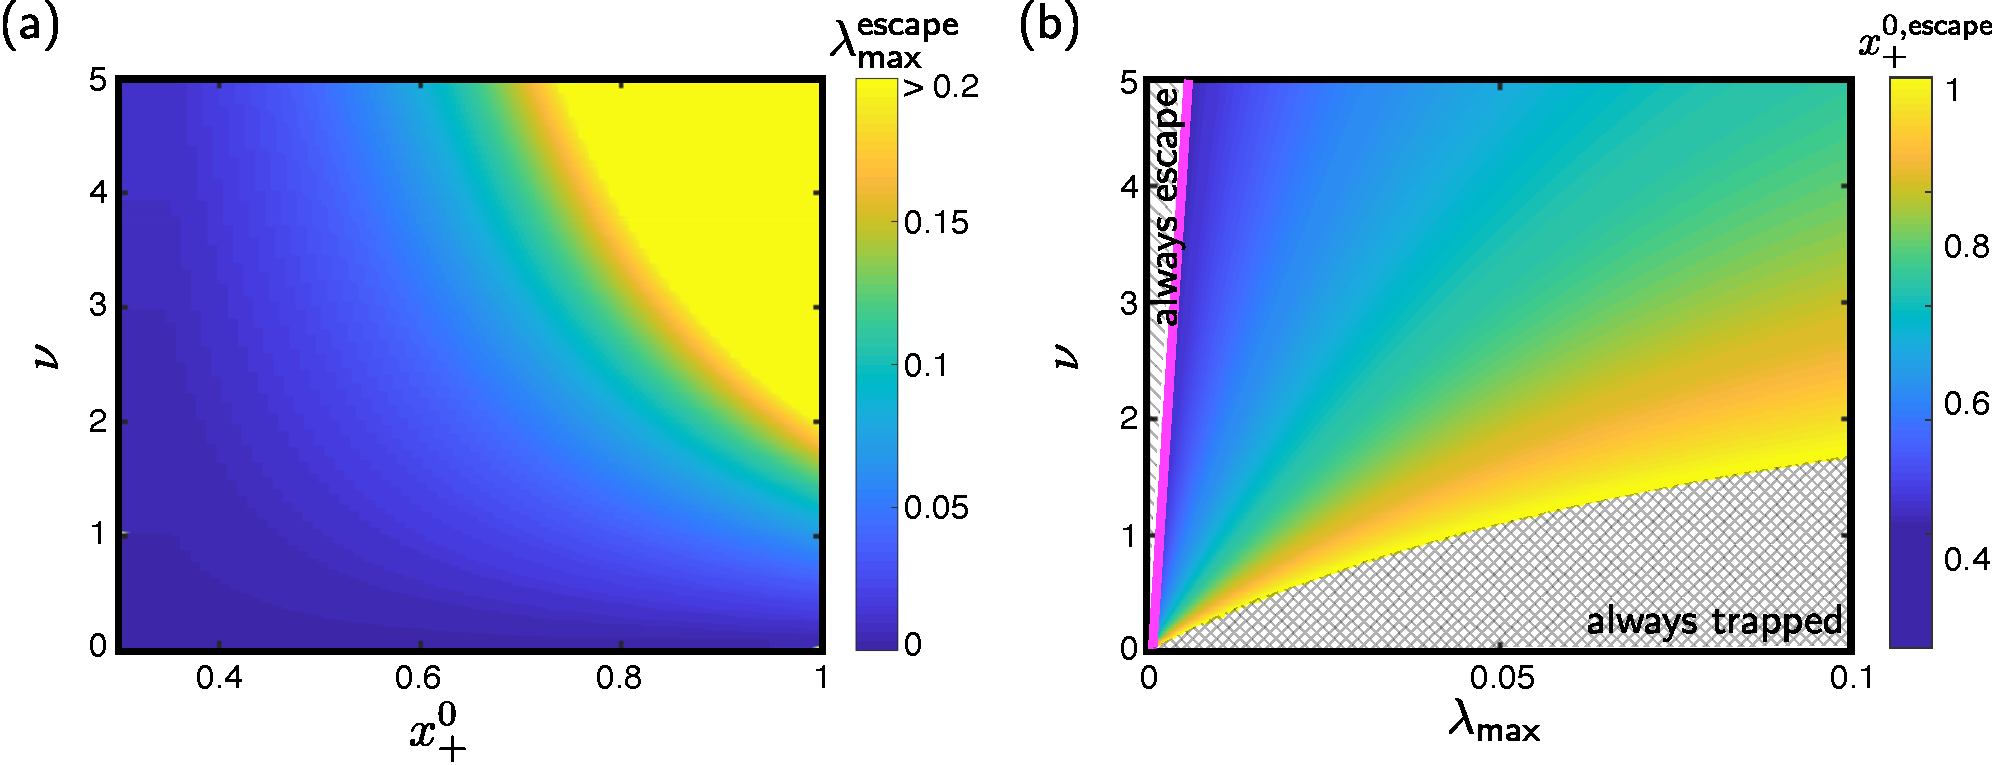
\includegraphics[width = \textwidth]{xright0_and_hysparmax_regime_diagram}
\caption{Predictions from the equilibrium calculation of (a) $\hysparmax^{\text{escape}}$ -- the largest value of $\hysparmax$ at which a droplet with initial position $\xright^0$ is able to escape -- and (b) $\xright^{0,\text{escape}}$ -- how far along the channel a droplet must start in order to escape if the contact angle hysteresis is $\hysparmax$. Both plots correspond to a droplet volume $V = 0.3$. Configurations with $(\hysparmax, \nu)$ that lie in the hatched region (bottom right) will trap droplets of volume $V = 0.3$, regardless of where they start in the channel. Similarly, $V = 0.3$ droplets will escape channels whose $(\hysparmax, \nu)$ lie in the striped region (top left), regardless of where they start in the channel; the pink line indicates the prediction~\eqref{E:Ch4:Hysteresis:MobileDroplets:always_escape_bdry} for the boundary of this `always escape' region.}\label{fig:xright_and_hyspar_regime_diagrams}
\end{figure}

The regime diagram in Figure~\ref{fig:xright_and_hyspar_regime_diagrams}(b)  (in $(\hysparmax, \nu)$ space) can be interpreted as a map showing how far along the channel the droplet must start in order to escape if the contact angle hysteresis if $\hysparmax$; we refer to this `escape position' as $\xright^{0,\textsf{escape}}$.
The equilibrium data for $V = 0.2$ are plotted as a surface in Figure~\ref{fig:Ch4:Hysteresis:escape_surface}; configurations with initial condition $\xright^0 < \xright^{0,\text{escape}}$ (i.e.~beneath this surface) will be trapped, and vice versa -- configurations with initial condition $\xright^0 \geq \xright^{\text{escape}}$ (above this surface) will escape. As expected, with higher hysteresis $\hysparmax$, droplets need to start closer to the free end to escape.

Using the equilibria to predict the $\xright^{0,\text{escape}}$ does not work, however, when such equilibria do not exist. There are two possibilities for configurations whose $(\nu, V, \hysparmax)$ lie in regions of parameter space in which no equilibria exist: if equilibria exist for values of $\hyspar_e$ below $\hysparmax$, then droplets will always be stuck in this channel (the droplet is never able to overcome pinning, since it would need to be located beyond $\xright^0 = 1$ to create enough deflection to do so). Otherwise droplets will always escape (see Figure~\ref{fig:xright_and_hyspar_regime_diagrams}(b) and Figure~\ref{fig:Ch4:Hysteresis:nu_dt_variousV}, which is as in Figure~\ref{fig:xright_and_hyspar_regime_diagrams}(b) for droplet volumes, $V = 0.1$, $0.2$, $0.4$, and $0.5$).

The shape of these `always trapped' regions demonstrate that when surface tension is very weak (small $\nu$) only a small contact angle hysteresis $\hyspar_{\text{max}}$ is needed to ensure that droplets always get stuck, as we might expect. In addition, the contact angle hysteresis needed to ensure that droplets are always trapped reduces for lower volume droplets (that are associated with smaller deflections).

The regions of parameter space in which droplets always escape are only appreciable for larger droplet volumes (note that for $V = 0.1$ and $V = 0.2$ in Figure~\ref{fig:Ch4:Hysteresis:nu_dt_variousV} this region does exist, but is not clearly visible on the scale of the plot). The border of these regions corresponds to equilibria with $\xlefteq = 0$, whose location we expressed analytically in~\eqref{E:Ch4:Hyseresis:Equilibria:Eqs:analytic_sol_volume}--\eqref{E:Ch4:Hyseresis:Equilibria:Eqs:analytic_sol_open_ends}; we therefore predict that droplets will always escape when
\begin{equation}\label{E:Ch4:Hysteresis:MobileDroplets:always_escape_bdry}
\nu > \frac{8}{V^4}\frac{\hyspar_{\text{max}}}{(1+\hyspar_{\text{max}})^2}\left(\frac{3\hyspar_{\text{max}} + 5}{5\hyspar_{\text{max}} + 5}\right)^4.
\end{equation}
The boundary between 'always escaping' and some trapping, given by equality in~\eqref{E:Ch4:Hysteresis:MobileDroplets:always_escape_bdry}, is included as the pink curves in Figure~\ref{fig:xright_and_hyspar_regime_diagrams}(b) and Figure~\ref{fig:Ch4:Hysteresis:nu_dt_variousV}. The sensitive dependence of~\eqref{E:Ch4:Hysteresis:MobileDroplets:always_escape_bdry} on $V$ elucidates why the `always escape' region is not resolved for smaller volume droplets.


\begin{landscape}
\begin{figure}[t]
\centering

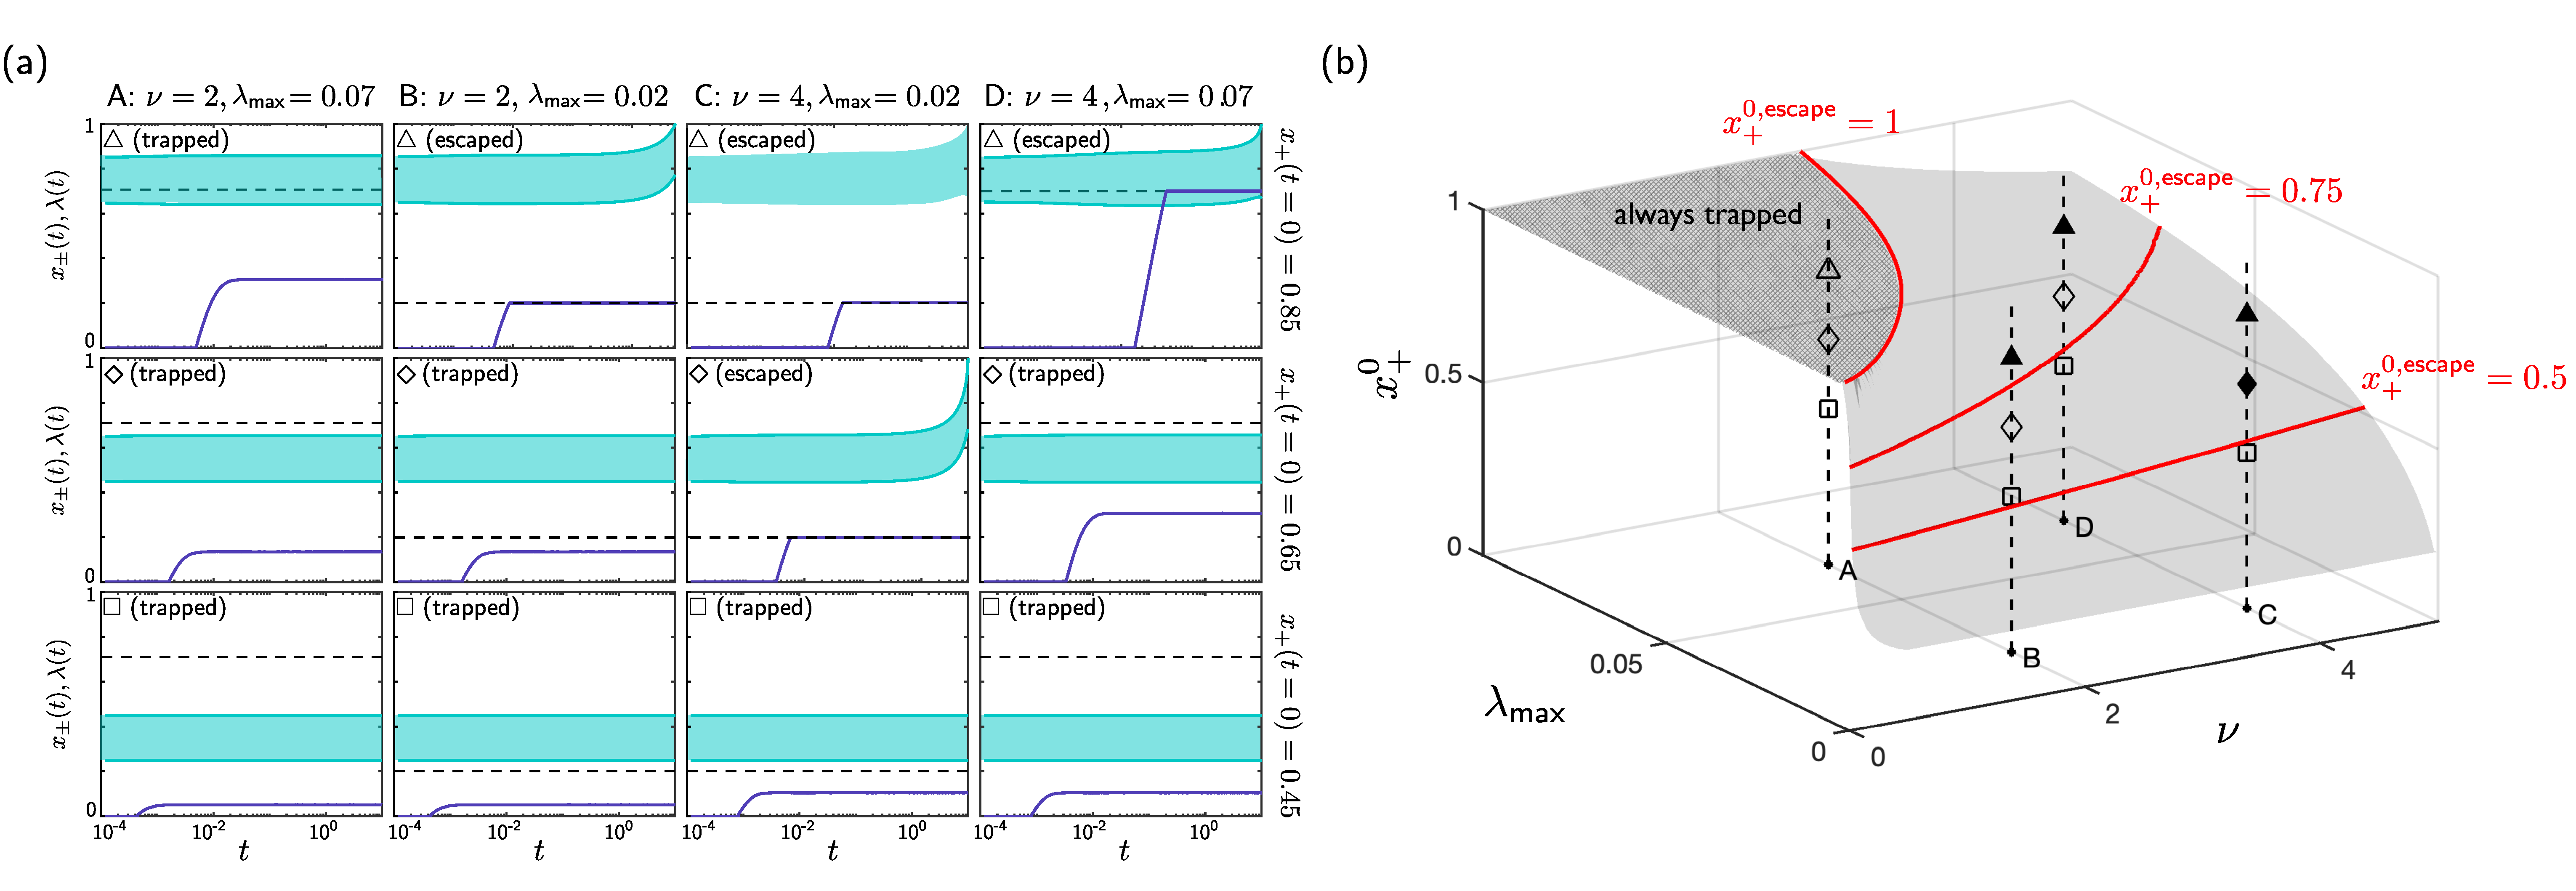
\includegraphics[scale = 0.22]{escape_surface_landscape}
\caption{(a)  Numerically obtained droplet trajectories (the portion of the channel occupied by the droplet is indicated by the green shaded region) as well as the contact angle difference asymmetry $\hyspar$ (purple curve) and contact angle hysteresis $\hyspar_{\text{max}}$ (dashed black line) corresponding to the parameter values at the marked locations (at symbols along dashed lines) in (b). (b) `Escape surface': surface plot of locations of equilibria with $V = 0.2$, interpreted as the boundary between regions of parameters space where droplets will be trapped (below the surface) and regions where droplets will escape (above the surface). Symbols indicate the fate of droplets that start with a particular $\xright^0$: $\triangle$: $\xright^0 = 0.85$, $\diamond$: $\xright^0 = 0.65$, $\square$: $\xright^0 = 0.45$. Filled symbols indicate droplets that escaped ($\hyspar$ reaches $\hysparmax$), open symbols indicate droplets that were trapped ($\hyspar$ does not reach $\hysparmax$).}\label{fig:Ch4:Hysteresis:escape_surface}
\end{figure}
\end{landscape}

\begin{figure}[h!]
\centering
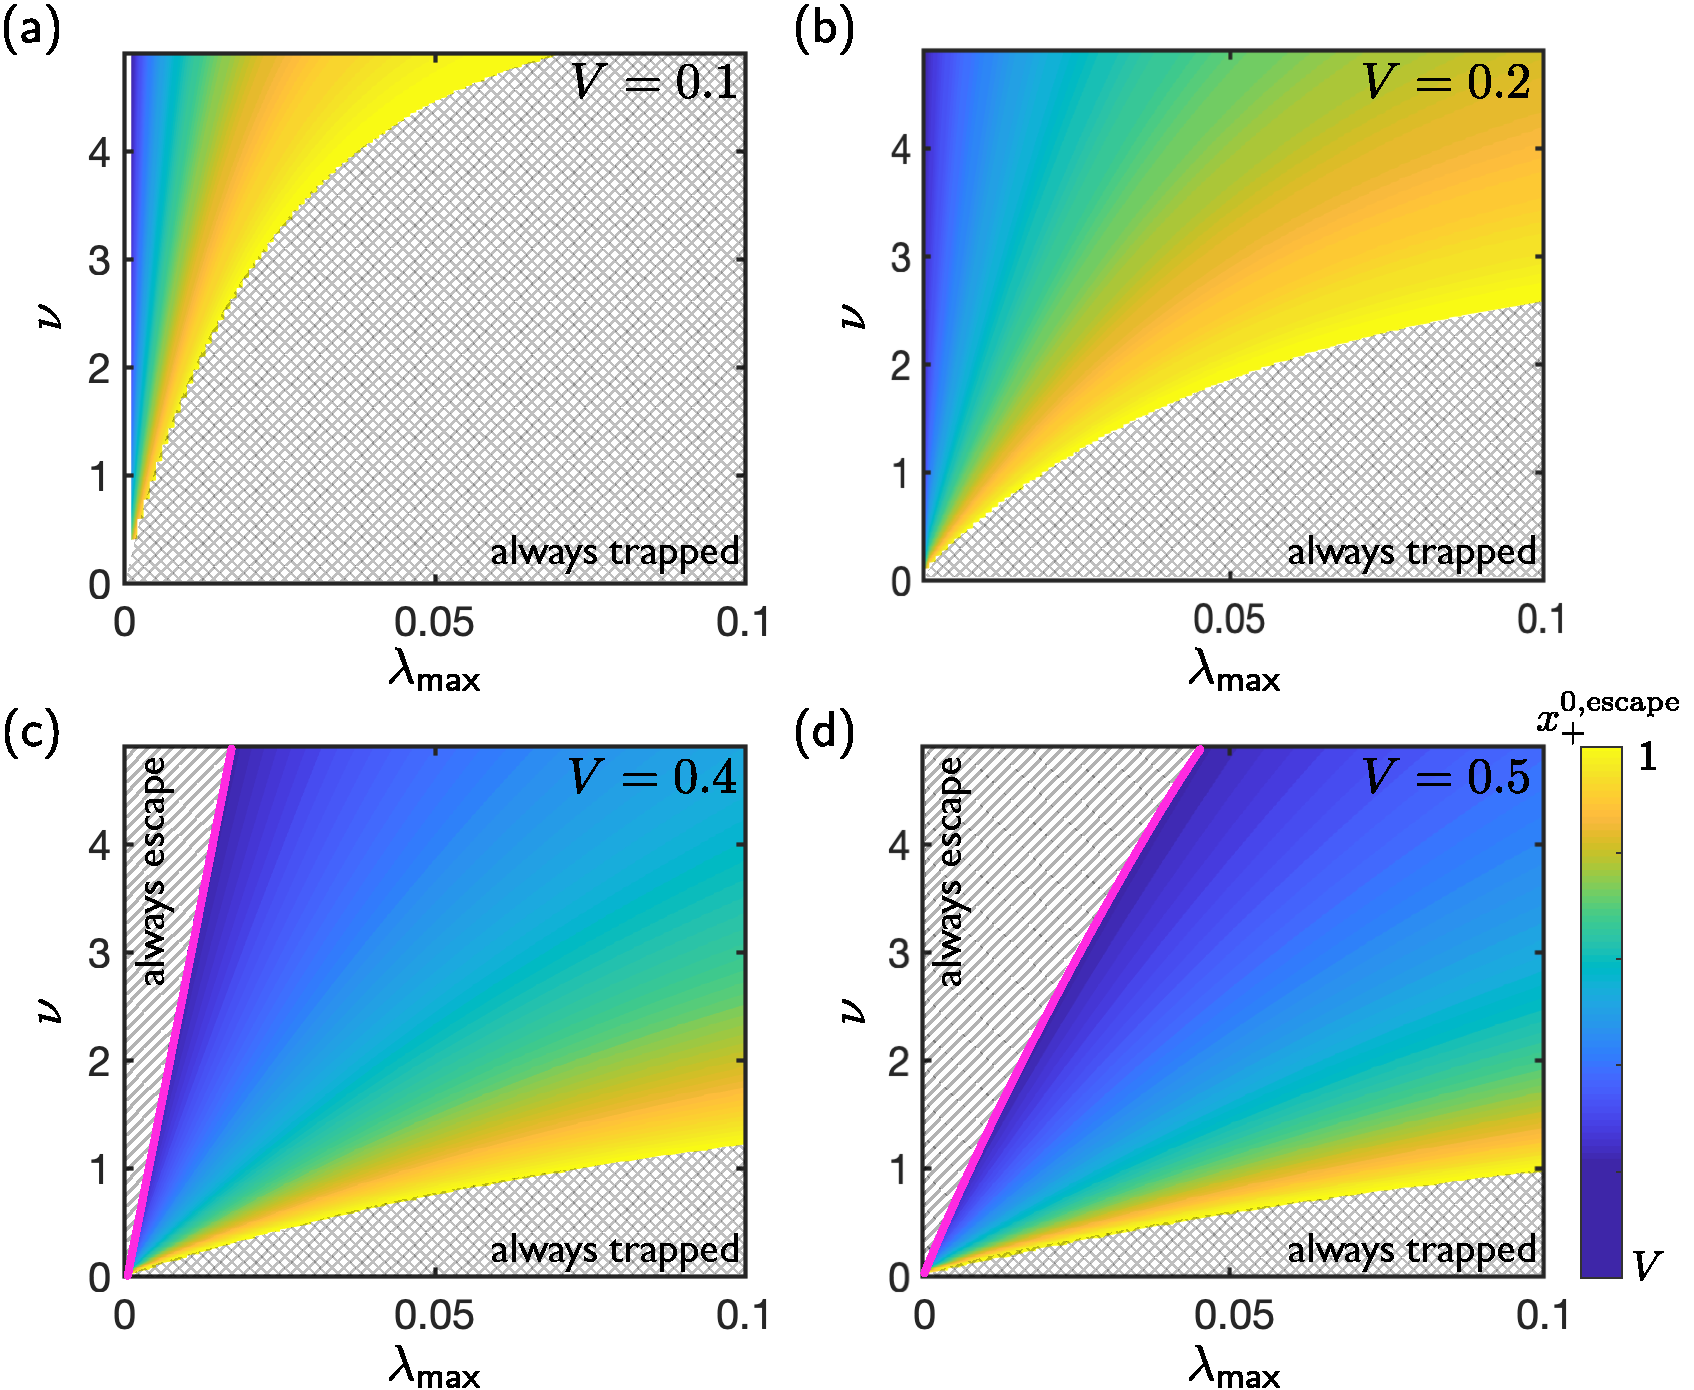
\includegraphics[width = 0.84\textwidth]{nu_dt_regime_diags_diffV}
\caption{Predictions from the equilibrium calculation of  $\xright^{0,\text{escape}}$ -- how far along the channel the droplet must start in order to escape if the contact angle hysteresis is $\hysparmax$ and bendability is $\nu$ (as in Figure~\ref{fig:xright_and_hyspar_regime_diagrams}(b)) for (a) $V = 0.1$, (b) $V = 0.2$, (c) $V = 0.4$, and (d) $V = 0.5$. The colour-bar applies in (d) applies to each plot with the appropriate value of $V$.  Configurations with $(\hysparmax, \nu)$ that lie in the hatched regions (bottom right of each plot) will trap droplets of the corresponding volume, regardless of where they start in the channel. Droplets will escape channels whose $(\hysparmax, \nu)$ lie in the striped region (top left of each plot), regardless of where they start in the channel. The pink line indicates the prediction~\eqref{E:Ch4:Hysteresis:MobileDroplets:always_escape_bdry} for the boundary of `always escape' region (in (a) and (b), this line covers the $y$-axis and is not shown).}\label{fig:Ch4:Hysteresis:nu_dt_variousV}
\end{figure}

%
\subsubsection{Comparison with full numerics}
We compare the results of our equilibrium-based predictions section with numerical results of the full (dynamic) model. To do so, we compute $\xright^{0,\text{escape}}$ numerically using a bisection scheme, with the model equations solved numerically for many different initial conditions. We use $\xright^0 = 0.97$ as a first upper bound to avoid the situation where the `$+$' meniscus is pushed onto the free end $x = 1$ during the initial squeezing; droplets that are trapped even for $\xright^0 = 0.97$ are said to be always be trapped. Similarly, we use $\xright^0 = V + 0.03$ (i.e.~ $\xleft^0 = 0.03$) as the first lower bound; droplets that escape even for $\xright^0 = V + 0.03$ are said to always escape.

The values of $\xright^{0,\text{escape}}$ obtained numerically in this way agree well with the values determined from  equilibrium calculation. This is shown in Figure~\ref{fig:Ch4:Hysteresis:numerics_comparison} where agreement would mean that the colour of the circles in the region where equilibria exist are indistinguishable from the background while the red circles (indicating where droplets never escaped) should be entirely within the empty region towards the right. Note that the numerically determined $\xright^{0,\text{escape}}$ are systematically lower than the equilibrium based predictions (although this is not clearly visible in Figure~\ref{fig:Ch4:Hysteresis:numerics_comparison}), because the equilibrium calculation does not account for the meniscus motion in the squeezing period.

\begin{figure}
\centering
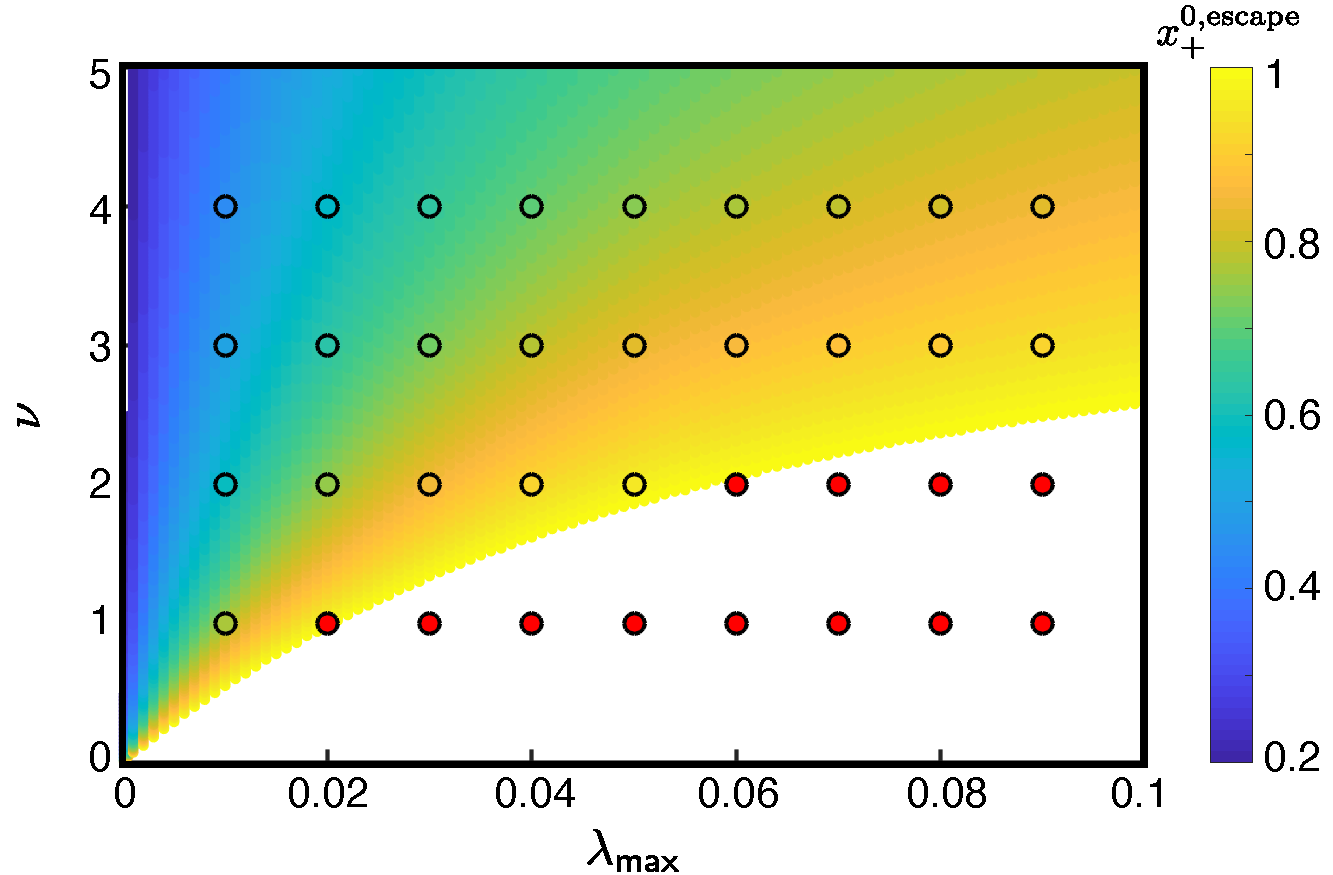
\includegraphics[width = 0.6\textwidth]{numerics_comparison}
\caption{Predictions from the equilibrium calculation (background colour) and numerical solutions of the model equations (circles) for $\xright^{0,\text{escape}}$ with $V = 0.2$. Red markers indicate configurations in which the droplet is always trapped in numerical solutions, regardless of its initial position.}\label{fig:Ch4:Hysteresis:numerics_comparison}
\end{figure}

\subsection{Non-wetting droplets}\label{S:Ch4:Hysteresis:NonWetting}
We conclude this section with a very brief presentation of the corresponding results for non-wetting configurations.

%it's basically the same
The dynamic behaviour of wetting and non-wetting configurations is qualitatively similar: assuming the droplet initially has receding angles at both menisci, an initial squeezing regime is followed by a period in which $\xleft$ is pinned and, possibly, a period in which the droplet translates. Again, droplets can only be trapped during the period for which $\xleft$ is pinned, and not whilst translating.

%here are the always escape and always trapped regions
The mechanism behind droplet trapping in the non-wetting case is exactly the same: in some regions of parameter space, the droplet must begin sufficiently far along the channel if it is to escape. In other regions of parameter space, droplets are trapped regardless of their initial position, and, in others still, they will escape regardless of their initial position; the boundaries between these regions (based on the equilibrium calculation) are indicated in Figure~\ref{fig:Ch4:Hysteresis:trapping_regions_nonwetting} for various droplet volumes $V$. The regions have a qualitatively similar shape to those in the corresponding wetting case (albeit with $\nu \to -\nu$, $\hyspar_{\text{max}} \to -\hyspar_{\text{max}}$); in particular, for small bendability, only a small amount of contact angle hysteresis is required to ensure that droplets are always trapped, and both the always trapped and always escape regions (the latter still given by~\eqref{E:Ch4:Hysteresis:MobileDroplets:always_escape_bdry}) are very sensitive to the value of $V$.

Interestingly, the symmetry $\nu \to -\nu$, $\hyspar_{\text{max}} \to -\hyspar_{\text{max}}$ is not quantitative: Figure~\ref{fig:Ch4:Hysteresis:trapping_regions_nonwetting} shows that the always trapped region is larger, and the always escape region is smaller, for non-wetting configurations than wetting configurations. Without going into detail, the non-linearity in the Laplace pressure boundary condition is responsible for this asymmetry: non-wetting droplets cannot create as large a droplet pressure, and thus deformation, while $\xleft$ is pinned because the meniscus pressure, which scales with $1/h$, does not change as sharply when advancing into an outward tapered channel (increasing $h$) than when advancing into an inward tapered channel (decreasing $h$).

\begin{figure}
\centering
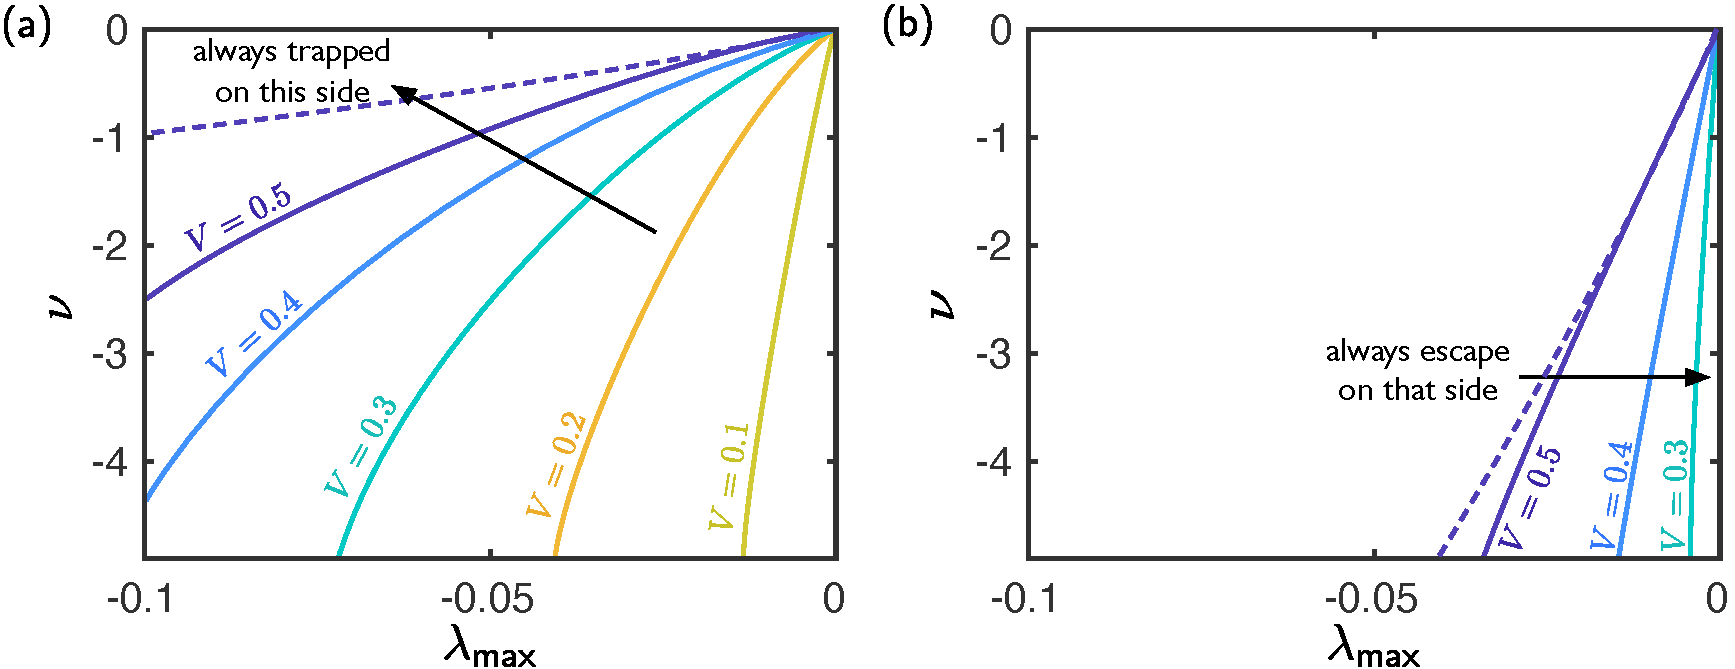
\includegraphics[width = 0.95\textwidth]{non_wetting_escape_and_trapped_regions}
\caption{Boundaries of the regions of $(\hysparmax, \nu)$ space in which (a) droplets are always trapped in the channel, regardless of their initial position, and (b) droplets always escape the channel, regardless of their initial position (based on locations of equilibria). Each boundary corresponds to a different droplet volume. Arrows indicate which side of the boundary droplets are always trapped or always escape, as appropriate. In both plots, the dashed purple curve shows the reflection $\nu \to -\nu, \hysparmax \to -\hysparmax$ of the corresponding boundary for wetting configurations with $V = 0.5$. }\label{fig:Ch4:Hysteresis:trapping_regions_nonwetting}
\end{figure}

\section{Summary}
In this chapter, we have consider two mechanisms through which droplets can be prevented from reaching the free end of the channel. Understanding when droplet motion to the free end of (and thus removal from) the channel is inhibited is important for self-cleaning surfaces that might exploit bendotaxis because trapped droplets might promote the sticky Wenzel state that we are aiming to avoid.

In the first half of the chapter, we considered geometric trapping, which describes the scenario in which the free ends of the channel contact before the droplet reaches the free end. We extended the model developed in Chapter 2 to describe the post-contact behaviour and studied the dynamics of the resulting model through numerical solutions of the model equations. The numerical solutions demonstrated the complex dynamics that result from the competition between the two modes of droplet motion -- squeezing and translating -- as well as from the competition between a diverging meniscus pressure and vanishing channel permeability. In particular, we saw that if the meniscus approaches the end of the channel while the channel walls are simply touching, it appears to reach the end in finite time, with asymptotic behaviour that is faster than previously reported for the analogous rigid case~\citep{Gorce2016Langmuir}. However, if the channel walls touch over an extended portion of their length (as we expect when surface tension is very strong), then the meniscus appears to take an infinite time to reach the cusp.

In the second half of this chapter, we considered trapping by contact angle hysteresis, whose strength is described in our model by the maximum contact angle asymmetry $\hysparmax = \cos \theta_r / \cos \theta_a -1$. Numerical solutions of the model equations confirmed our intuition that when hysteresis is sufficiently strong ($\hysparmax$ sufficiently large), droplets may be trapped in equilibrium part way along the channel. By studying steady solutions of the model equations and assessing their linear stability, we determined that these equilibria are stable and also that droplets will not translate to equilibrium (if droplets start to move appreciably along the channel, they will not be stopped). We identified the importance of the quantity $\hyspari$, the contact angle asymmetry required to hold the droplet in the pinned state (when equilibria are possible). $\hyspari$ gives a simple criterion for whether a droplet will escape: droplets in channels with initial conditions such that the maximum contact angle asymmetry $\hysparmax \leq \hyspari$ will escape, while those with $ \hysparmax > \hyspari$ will not. In reality, $\hyspari$ can only be determined by a full dynamic simulation, but our analysis of equilibria gives  an approximation for $\hyspari$. This approximation allowed us to re-purpose our regime diagrams, that  demonstrate where equilibria exist, to describe whether droplets of given parameters will be trapped or not. In doing so, we identified regions of parameter space in which droplets will always escape and other regions in which droplets are always trapped, regardless of where they start in the channel.  The shape of these regions agreed with our intuition, demonstrating that when the channel bendability is small, only a small amount of contact angle hysteresis is required to trap droplets. In addition, they confirmed that droplets are more likely to be trapped in channels with higher hysteresis, which emphasizes the need to minimize hysteresis in any superhydrophobic surface that might exploit bendotaxis. 


\begin{subappendices}
%\addcontentsline{toc}{section}{Appendices}
\renewcommand{\thesection}{\Alph{section}}
%\appendix

\section{Solving the equations for equilibria}\label{A:Ch4:FindingEquilibria}
In this appendix we describe the method used to find solutions of equations~\eqref{E:Ch4:Hyseresis:Equilibria:Eqs:Beam1}--\eqref{E:Ch4:Hyseresis:Equilibria:Eqs:Volume} describing an equilibrium configuration $h_e(x)$ whose menisci are located at $x = \xpmeq$.

We first `integrate out' the dry regions to give an equivalent problem defined only on the drop region $\xlefteq < x < \xrighteq$ with the effect of the dry regions encoded by effective boundary conditions (as discussed in \S2.2 and \S4.1 for the dynamic problem). In this droplet only problem, the ordinary differential equations, boundary conditions at $x = \xlefteq$ and volume constraint are independent of the nature of any contact at the wall ends (and hence identical for each of the three regimes). We have:
\begin{equation}\label{A:E:Ch4:FindingEquilibria:beam}
\dd{^4 h_e}{x^4} = p_0
\end{equation}
where
\begin{equation}\label{A:E:Ch4:FindingEquilibria:p0}
p_0 =- \frac{\nu}{h_e(\xrighteq)} = - \frac{\nu(\hyspar_e+1)}{h_e(\xlefteq)} \qquad \xlefteq < x< \xrighteq,
\end{equation}
\begin{align}
\left.\dd{^2 h_e}{x^2} - \frac{2}{\xlefteq^2}\left(2\xlefteq \dd{h_e}{x} - 3h_e+3\right)\right|_{x = \xlefteq} &= 0, \label{A:E:Ch4:FindingEquilibria:EffBC_xl1}\\
\left.\dd{^3 h_e}{x^3} - \frac{6}{\xlefteq^3}\left(\xlefteq \dd{h_e}{x} - 2h_e+2\right)\right|_{x = \xlefteq} &= 0.\label{A:E:Ch4:FindingEquilibria:EffBC_xl2}
\end{align}
\begin{equation}\label{A:E:Ch4:FindingEquilibria:Volume}
V = \int_{\xlefteq}^{\xrighteq}h_e(x)~\mathrm{d}x.
\end{equation}
The boundary conditions at $x = \xrighteq$ do depend on the nature of any contact at $x = 1$. For channels in regime I, we have boundary conditions
\begin{equation}\label{A:E:Ch4:FindingEquilibria:EffBC_xu_regimeI}
\dd{^2 h_e}{x^2}  = \dd{^3 h_e}{x^3} =0
\end{equation}
at $x = \xrighteq$. For channels in regime II, we have boundary conditions
\begin{equation}\label{A:E:Ch4:FindingEquilibria:EffBC_xu_regimeII}
(\xrighteq - 1)^3\dd{^3 h_e}{x^3}  - 3\left[(\xrighteq - 1)\dd{h_e}{x} - h_e\right] =
(\xrighteq - 1)\dd{^3 h_e}{x^3}  -\dd{^2 h_e}{x^2} = 0
\end{equation}
at $x = \xrighteq$. For channels in regime III, we have boundary conditions
\begin{equation}\label{A:E:Ch4:FindingEquilibria:EffBC_xu_regimeIII}
\dd{^2 h_e}{x^2} - \frac{6h_e}{(\xrighteq - \xceq)^2} = \dd{^3 h_e}{x^3} - \frac{6h_e}{(\xrighteq - \xceq)^3}=0
\end{equation}
at $x = \xrighteq$, where
\begin{equation}\label{A:E:Ch4:FindingEquilibria:EffBC_xu_regimeIII_xc}
\xrighteq - \xceq - \frac{h_e}{3}\left(\dd{h_e}{x}\right)^{-1}=0.
\end{equation}

For  given $V, \nu$ and $\hyspar_e$, the problem~\eqref{A:E:Ch4:FindingEquilibria:beam}--\eqref{A:E:Ch4:FindingEquilibria:EffBC_xu_regimeIII_xc} for $h_e(x), \xpmeq$ is nonlinear and therefore expensive to solve numerically. It is more convenient to instead specify a meniscus position (typically $\xlefteq$) and solve for $h_e(x)$ and $\xrighteq$ only,  computing the associated volume $V$ a posteriori; with $\xlefteq$ specified the problem~\eqref{A:E:Ch4:FindingEquilibria:beam}--\eqref{A:E:Ch4:FindingEquilibria:EffBC_xu_regimeIII_xc} can be converted into a polynomial in $\xrighteq$ (described below), which is computationally inexpensive to solve.  By sweeping over all permissible values of $\xlefteq$, we pick up all possible equilibria.

In the following sections, we give relevant details of this procedure which differ slightly for channels in regimes I \& II and channels in regime III. We therefore consider these cases separately.

Before we do so, we note that, regardless of the boundary conditions applied at the non-clamped end, the channel shape in the drop region may be expressed as
\begin{equation}\label{A:E:Ch4:FindingEquilibria:Shape}
h_e(x) = \frac{p_0}{24}(x - \xright)^4 + K_3 (x- \xright)^3 + K_2 (x- \xright)^2 + K_1 (x- \xright) + K_0
\end{equation}
where $K_i = K_i(\xrighteq, \xlefteq, p_0),~ i = 1,2,3,4$.
\subsection{Regimes I and II}
The boundary conditions~\eqref{A:E:Ch4:FindingEquilibria:EffBC_xu_regimeI} and~\eqref{A:E:Ch4:FindingEquilibria:EffBC_xu_regimeII} that apply for channels in regime I and II are linear. As a result, the coefficients $K_i, ~i = 1,2,3,4$ in~\eqref{A:E:Ch4:FindingEquilibria:Shape} are linear in the in the equilibrium pressure $p_0$ and multinomials in $\xpmeq$. Using the solution~\eqref{A:E:Ch4:FindingEquilibria:Shape},  the channel displacement at the menisci can be expressed as
\begin{align}
h_e(\xrighteq) &= f_+(\xlefteq, \xrighteq) + p_0 g_+(\xlefteq, \xrighteq), \label{A:E:Ch4:FindingEquilibria:Regime1_and_2:meniscus_disp_1}\\
h_e(\xlefteq) &= f_-(\xlefteq, \xrighteq) + p_0 g_-(\xlefteq, \xrighteq)\label{A:E:Ch4:FindingEquilibria:Regime1_and_2:meniscus_disp_2}
\end{align}
where $f_{\pm}, g_{\pm}$ are known (albeit regime dependent) multinomials.

Inserting~\eqref{A:E:Ch4:FindingEquilibria:Regime1_and_2:meniscus_disp_1}--\eqref{A:E:Ch4:FindingEquilibria:Regime1_and_2:meniscus_disp_2} into the two pressure conditions~\eqref{A:E:Ch4:FindingEquilibria:p0} gives two quadratic equations for the pressure $p_0$:
\begin{align}
p_0 \left[f_+(\xlefteq, \xrighteq) + p_0 g_+(\xlefteq, \xrighteq)\right]  &= -\nu, \label{A:E:Ch4:FindingEquilibria:pressure_quadratic1}\\
 p_0 \left[f_-(\xlefteq, \xrighteq) + p_0 g_-(\xlefteq, \xrighteq)\right]  &= -\nu ( \hyspare+1).\label{A:E:Ch4:FindingEquilibria:pressure_quadratic2}
\end{align}
Eliminating $p_0$ from~\eqref{A:E:Ch4:FindingEquilibria:pressure_quadratic1}--\eqref{A:E:Ch4:FindingEquilibria:pressure_quadratic2} gives a single multinomial whose coefficients depend on parameters $\nu, \hyspare$:
\begin{equation}\label{A:E:Ch4:FindingEquilibria:master_quadratic}
F(\xlefteq, \xrighteq;\nu, \hyspare) = 0.
\end{equation}
Under our assumption that $\xlefteq$ is prescribed, \eqref{A:E:Ch4:FindingEquilibria:master_quadratic} is simply a polynomial equation for $\xrighteq$ (of degree 9 for regime I configurations, and degree 19 for regime II configurations). We solve this polynomial numerically using the \textsc{matlab} routine \texttt{roots}, which computes the eigenvalues of the matrix whose characteristic polynomial is given by~\eqref{A:E:Ch4:FindingEquilibria:master_quadratic}.

Once the equation~\eqref{A:E:Ch4:FindingEquilibria:master_quadratic} has been solved for $\xrighteq$, we keep only those roots that correspond to physically relevant solutions -- i.e. those with $\xlefteq < \xrighteq < 1$ and for which the open end condition~\eqref{E:Ch4:Hyseresis:Equilibria:Eqs:regimeI_constraint} (for channels in regime I), or the repulsive shear and negative slope conditions~\eqref{E:Ch4:Hyseresis:Equilibria:Eqs:regimeII_constraint} (for channels in regime II) are satisfied.

\subsection{Regime III}
The procedure is a little more complicated for configurations in regime III because the boundary conditions~\eqref{A:E:Ch4:FindingEquilibria:EffBC_xu_regimeIII}--\eqref{A:E:Ch4:FindingEquilibria:EffBC_xu_regimeIII_xc} are not linear. As a result, the system of equations for the $K_i$ in~\eqref{A:E:Ch4:FindingEquilibria:Shape} that emerge from  using~\eqref{A:E:Ch4:FindingEquilibria:EffBC_xl1}--\eqref{A:E:Ch4:FindingEquilibria:EffBC_xl2} and~\eqref{A:E:Ch4:FindingEquilibria:EffBC_xu_regimeIII}--\eqref{A:E:Ch4:FindingEquilibria:EffBC_xu_regimeIII_xc} are non-linear in $p_0$. After inserting the result  into the pressure conditions~\eqref{A:E:Ch4:FindingEquilibria:p0} we obtain a system of two quartic equations for the pressure $p_0$.

To obtain solutions of these quartics (for a given $\xlefteq$), we first specify a meniscus position $\xrighteq$ and solve (independently) the resulting quartics in $p_0$. We choose the pair ($\xlefteq, \xrighteq$), and the corresponding pressure $p_0$, to be a candidate equilibrium if any of the roots $p_0$ of the first quartic coincide (to within a tolerance) with any of the roots of the other quartic (we typically choose a tolerance of $0.1$, which is large enough to ensure that we do not miss any solutions but small enough that the search space for the following non-linear solver is not too large). By removing any un-physical roots, and looping over all possible $\xlefteq$, we are left with a set of candidate solutions $\{(\xlefteq^i, \xrighteq^i, p_0^i)\}, ~i =1,\dots, n$.

To find exact solutions of the equilibrium equations, we solve the non-linear equations using \textsc{matlab}'s non-linear equation solving routine \texttt{fsolve}. We provide \texttt{fsolve} with an initial guess at each of the candidate solutions.

Finally, once every possible equilibria has been found in this way, we remove any that violate the sticking condition~\eqref{E:Ch4:Hyseresis:Equilibria:Eqs:regimeIII_constraint}.


\end{subappendices}
}
\graphicspath{{./Sections/Chapter5_instability/figures/}}
\newcommand{\poisson}{\eta} %Poisson's ratio of the channel walls
\newcommand{\aspect}{a} %aspect ratio: \aspect = [z]/[y]
\newcommand{\jump}[1]{_{#1-}^{+}} %jump conditions across interface
\newcommand{\amplitude}{\delta} %amplitude of perturbation in scaling

%dimensionless variables: uncomment below to leave hats on
 \renewcommand{\familydefault}{\sfdefault}

%\newcommand{\h}{\hat{h}}
%\newcommand{\x}{\hat{x}}
%\newcommand{\y}{\hat{y}}
%\newcommand{\that}{\hat{t}}
%\newcommand{\nablahat}{\hat{\nabla}}

\newcommand{\h}{h}
\newcommand{\x}{x}
\newcommand{\y}{y}
\newcommand{\that}{t}
\newcommand{\nablahat}{\nabla}

%for use in the small deformation asymptotics
\newcommand{\X}{X} %for the asymptotics when rescaling with V
\renewcommand{\K}{K} %rescaled wavenumber

\newcommand{\GG}{\psi} %perturbation size after rescaling with nu V^3 (the size of the shear term)
\newcommand{\GGG}{\upsilon} %perturbation pressure rescaling with nu V^3 (the size of the shear term)
\chapter{Bendo-capillary instability of a channel}

In this chapter, we extend the work of the rest of this thesis to consider channels that vary in the third spatial direction.

As motivation, we consider the experiment described in \S 1.4.4 (shown again in Figure~\ref{fig:InstabilityChapter:Intro:ExptSnapshots}(a)). Recall that in these experiments, droplets nucleate at the base of a three-dimensional array of channels and their upper surface moves towards the free end of the channels (the ends closest to the camera, see Figure~\ref{fig:InstabilityChapter:Intro:ExptSnapshots}) in a process reminiscent of bendotaxis. As this takes place, a periodic pattern emerges in the in-plane direction (we refer to variations in the plane parallel to the undeformed channel walls as being `in-plane', and variations in the across channel plane as being `transverse', see Figure~\ref{fig:InstabilityChapter:Intro:ExptSnapshots}(b)). This pattern emerges at relatively early times, and persists throughout the experiment (visible in Figure~\ref{fig:InstabilityChapter:Intro:ExptSnapshots}(a)3--6); its periodicity suggests a preferential wavelength for growth in the transverse direction. We therefore turn now to a first study of this instability.

We focus on three key questions in this chapter: Is the growth of periodic perturbations a generic feature of bendo-capillary systems in which transverse bending and flow are allowed? If so, which physical processes control the wavelength that emerges? And, how does the addition of liquid via condensation mediate this mode selection?


\begin{figure}[h]
\centering
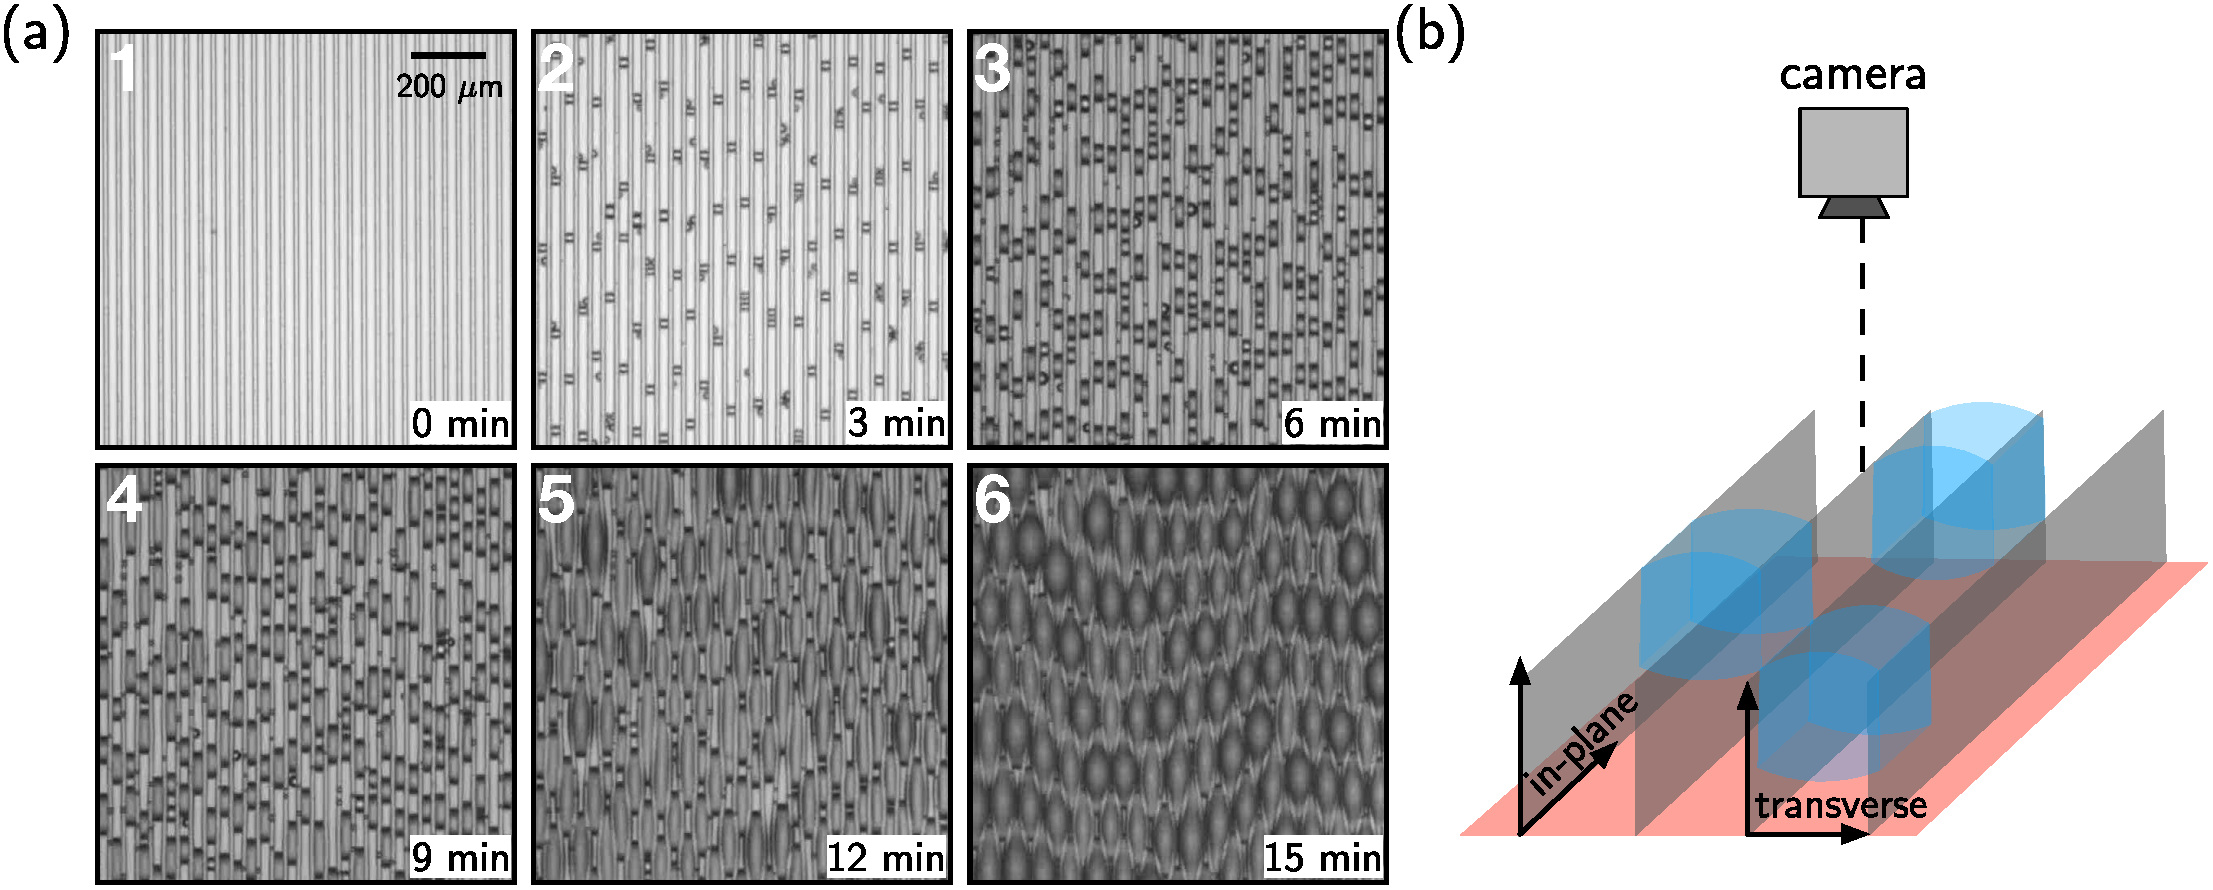
\includegraphics[width = \textwidth]{BrinkmannExperiments}
\caption{(a) Snapshots of experiments performed by~\cite{Seemann2011JPhysCondMat} in which liquid droplets condense within an array of deformable microchannels and eventually reach the free end of the channel. Notice how the emergent periodic pattern appears at relatively early times. (b) Schematic diagram of the experiments shown in (a). We refer to variations in the plane parallel (perpendicular) to the channel walls as in-plane (transverse, respectively), as indicated}
\label{fig:InstabilityChapter:Intro:ExptSnapshots}
\end{figure}

This chapter is structured as follows. In the first section, we describe (our hypothesis for) the mechanism driving the `weaving' instability responsible for the pattern formation, and then gain physical insight via a scaling argument. In the third section, we develop a mathematical model for a simple bendo-capillary system which may be susceptible to the instability. The remainder of the chapter is dedicated to  studying the mode selection process; initially we focus on the case when the liquid volume is constant, before considering the effect of adding liquid volume via condensation.


\section{Mechanism}
We hypothesize that the periodic pattern seen in Figure~\ref{fig:InstabilityChapter:Intro:ExptSnapshots} is the result of an instability, with the observed wavenumber of instability determined as that of the fastest growing mode. In this chapter, we investigate the possibility that this preferred mode is determined by a competition between interfacial curvatures in the transverse and in-plane directions (which we refer to as a `competing-curvature' instability).

\subsection{Competing curvature instabilities: Rayleigh-Plateau}

%how does perturbation change curvatures
The canonical example of a competing-curvature instability is the Rayleigh-Plateau instability~\citep{Plateau1873, Rayleigh1879PRSL, Rayleigh1892PhilosMag}: in the absence of gravity, a thin thread of liquid of uniform radius $r$  may remain in equilibrium (Figure~\ref{fig:InstabilityChapter:Mechanism:Mechanism}(a)) since the constant pressure this requires is consistent with the constant pressure difference across a meniscus of constant curvature.
If the interface is disturbed slightly by an axisymmetric perturbation, periodic in the in-plane direction the transverse curvature -- inversely proportional to the local radius of the thread -- increases (decreases) at troughs of lower radius (peaks of higher radius, respectively). The opposite is true of the in-plane curvature, which is negative at (locally) concave troughs and positive at convex peaks (Figure~\ref{fig:InstabilityChapter:Mechanism:Mechanism}(a)). The difference in the in-plane curvature between peaks and troughs increases from zero with the wavenumber, while the difference in the transverse curvature is independent of it.  As a result, perturbations with sufficiently small wavenumbers (specifically $k < 1/r$) result in a decrease (increase) in the total curvature -- and hence pressure -- at peaks (troughs, respectively), resulting in liquid being driven from troughs to peaks and thus amplifying the perturbation.

\begin{figure}[t]
\centering
\includegraphics[width = \textwidth]{mechanism_png_subfigs}
\caption{Air-liquid interfaces in competing-curvature instabilities. (a)(Left) A thread of liquid with radius $r$ has interfacial curvatures $\kappa_{\parallel}$ and $\kappa_{\perp}$ in the in-plane and transverse directions, respectively (the schematic diagram indicates the orientation of the planes).  (Right) The pressure differences associated with the variable curvatures following a perturbation drives fluid from high to low transverse curvature, leading to the Rayleigh-Plateau instability. (b)-(d) Schematic diagrams of the interface between liquid and air in a narrow channel. The interface has curvature components $C_{\perp}$ and $C_{\parallel}$ (taken in the same planes as in (a)). The base state (b) has no in-plane curvature. The effect of perturbing the interface from the base state differs between (c) rigid, tapered and (d) flexible channels. Arrows indicate the local curvature changes, relative to the base state.}
\label{fig:InstabilityChapter:Mechanism:Mechanism}
\end{figure}


\subsection{The Effect of confinement: Al-Housseiny}
If the liquid is confined between two plates with a gap thickness that varies in the transverse direction (Figure~\ref{fig:InstabilityChapter:Mechanism:Mechanism}(b),(c)), a competing curvature instability is also possible.  (Note that confinement can alter mode selection in the Rayleigh-Plateau instability if the liquid does not contact the walls but is surrounded by a second liquid~\citep{Son2003Macromolecules}, but we do not consider this scenario here.) In the confined case, the stable configuration is a uniform advancing front with no in-plane curvature, $C_{\parallel} = 0$. The key difference between this scenario and the free interface is that here the confinement sets the transverse curvature; the total curvature of the base state is  $C(x) = C_{\parallel}  + C_{\perp} =  C_{\perp} = -2 \cos \theta/h(x)$~\citep{deGennes2004}, where $h(x)$ is the (non-constant) channel thickness, $\theta$ is the contact angle between the liquid and the plates, and the $x$-axis is aligned along the channel  (Figure~\ref{fig:InstabilityChapter:Mechanism:Mechanism}(b)).

Consider first a wetting configuration, $\theta < 90$\si{\degree}. Provided the channel is narrowing, a periodic perturbation to the interface (Figure~\ref{fig:InstabilityChapter:Mechanism:Mechanism}(c)) decreases the channel width at protrusions (where the liquid advances ahead of the original meniscus position) and thus increases the magnitude of the transverse curvature  $C_{\perp}$ there (corresponding to a more negative capillary pressure). Invaginations experience a decrease in the magnitude of the transverse curvature, and hence a reduction in the suction pressure, owing to the weaker confinement. As a result, protrusions may suck liquid from invaginations, thus increasing the size of the perturbation and destabilizing the interface.

As in the Rayleigh-Plateau instability, the transverse curvature changes are in competition with the in-plane curvature $C_{\parallel}$, which offers a stabilizing effect whose strength increases with wavenumber. Again, perturbations of a sufficiently small wavenumber are amplified (the range of unstable wavenumbers depends on the contact angle, and the local channel thickness and tapering angle). This scenario has been studied in detail (both theoretically and experimentally) in recent years~\cite[see][for example]{Protiere2010EPL, AlHousseiny2012NaturePhysics,AlHousseiny2013PhysFlu,Keiser2016JFM, LedesmaAguilar2017SoftMatter}.

If the liquid does not wet the channel ($\theta> 90\si{\degree}$), protrusions (invaginations) of a perturbation to the meniscus experience a decrease (increase, respectively) in transverse curvature, provided the channel is widening; the convex interface experiences a weaker (stronger) confinement. Again, perturbations of sufficiently small wavenumber will be amplified. We stress that this instability is only possible for non-wetting configurations if the channel is widening (in the direction of advancing interface) and only possible for wetting configurations if the channel is narrowing.

%I don't think I need to mention confined RP instability (e.g. Tomotika, 1935 and Son, 2003): they're not looking at contact.

\subsection{Introducing elasticity}\label{S:InstabilityChapter:Mechanism:Elasticity}
If the tapered wall is not rigid but deforms in response to liquid pressure (Figure~\ref{fig:InstabilityChapter:Mechanism:Mechanism}(d)), the picture changes in two important ways. Firstly, the global tapering of the channel is set by the bulk liquid pressure. With the familiar clamped-free conditions on the beams, the induced tapering will always be in the direction that favours instability: wetting configurations will be tapered inwards, and non-wetting configurations will be tapered outwards. This means that, unlike the rigid case, it is possible that both wetting and non-wetting configurations will be susceptible to the bendo-capillary competing curvature instability within the same channel.

The second important difference with the competing curvature instability in a rigid confinement it that a meniscus perturbation will result in an additional elastic response from the channel. Protrusions will apply a pressure over a longer portion of the channel, compared to the flat base state, resulting in an enhanced wall response; the confinement that a protrusion experiences will be exacerbated (and the confinement an invagination experiences will be reduced) by the elastic response to the perturbation. This, in turn, will lead to a greater difference in the destabilizing transverse curvature between meniscus protrusions and invaginations. We anticipate that this may extend the range of unstable modes, or make the growth rate faster, than the corresponding rigid case.


\section{Scaling argument}\label{S:InstabilityChapter:Scaling}

Before developing a detailed model, we seek first to gain some quantitative insight into mode selection driven by the mechanism described in \S\ref{S:InstabilityChapter:Mechanism:Elasticity}. We consider the configuration shown in Figure~\ref{fig:InstabilityChapter:SlowCondensation:Scaling:ToyProblem}: a section of a channel with width $\lambda$ and length $L$ contains liquid sat at a rigid base of thickness $2H$, while the opposite end is open. The other two walls of the channel are narrow and flexible; they bend in response to the liquid pressure (characterized by a bending stiffness $B$), but for simplicity we allow them to bend only along their length (i.e.~in the transverse direction). They are clamped at the rigid base. We imagine a cut along the centre of each deformable wall (black dashed lines in Figure~\ref{fig:InstabilityChapter:SlowCondensation:Scaling:ToyProblem}), so that the two halves can deform independently of one another. In effect, we allow liquid to flow between the two halves of the (section of) channel, whilst neglecting in-plane bending. (Any instability that appears in this system will be a discrete square wave instability.)

\begin{figure}[t]
\centering
\includegraphics[width = \textwidth]{Scaling_3d}
\caption{Schematic diagrams of section of a flexible channel consisting of a solid base and two flexible walls, which are only permitted to bend along their length. A cut along each of the flexible walls (black dashed line) allows the two halves to bend independently. (a) The system is in equilibrium with the meniscus located a distance $x_m$ from the base.  (b) The equilibrium is perturbed by moving the menisci on either side of the cut a distance $\delta$; if $\lambda$ is sufficiently large, this perturbation results in the flow of liquid from troughs (blue) to peaks (red) with speed $U$, amplifying the perturbation, as described in the main text.}
\label{fig:InstabilityChapter:SlowCondensation:Scaling:ToyProblem}
\end{figure}

For the moment, we assume that the fraction of the channel occupied by liquid is relatively small. (This is the situation at early times in the condensation experiments that motivate this work; pattern formation first occurs in these early stages.) In this simple argument, we assume that no condensation occurs in the time interval of interest: the amount of liquid in the channel remains constant.

To make the analysis presented in this chapter more tractable, we consider the situation in which the condensed liquid remains in contact with the base. In this case, a two-dimensional equilibrium exists~\citep{Taroni2012JFM}.

Consider such an equilibrium configuration in which the meniscus is located a distance $x_m$ from the clamped base. As the volume of liquid is relatively small, the walls are not deformed significantly and the channel half-width at the meniscus $h_m \sim H$ (see Figure~\ref{fig:InstabilityChapter:SlowCondensation:Scaling:ToyProblem}(a)). By conservation of mass, the meniscus position is $x_m \sim \Omega / H$, where $\Omega$ is the cross sectional volume. The liquid pressure in this configuration is $p_m \sim -\gamma \cos \theta/H$, where $\gamma$ is the surface tension coefficient of the liquid, and $\theta$ the contact angle between the liquid and channel wall.

Before we consider perturbations to this equilibrium, we need a scaling for $h_m'$, the channel slope at the meniscus. By considering a cantilever beam with bending stiffness $B$ bending over a length scale $x_m$ by a uniform (Laplace) pressure $-\gamma \cos \theta / H$ we find~\citep{Timoshenko1959},
\begin{equation}\label{E:InstabilityChapter:Scaling:hmprimed}
h_m' \sim -\frac{\gamma \cos \theta x_m^3}{B H}.
\end{equation}

We mimic a periodic perturbation of wavenumber $k = 2\pi/\lambda$, and amplitude $\amplitude$, by considering a region of length $\lambda$, with each split region having length $\lambda/2$ (as in f
Figure~\ref{fig:InstabilityChapter:SlowCondensation:Scaling:ToyProblem}). We then force one side of the cut to advance (uniformly) to $x_0 + \amplitude$ and the other to retreat to $x_0 - \amplitude$ (Figure~\ref{fig:InstabilityChapter:SlowCondensation:Scaling:ToyProblem}(b)). As discussed, the transverse interfacial curvature, and thus liquid pressure, changes as a result of this perturbation: the transverse curvature changes as the interface is forced into a stronger (or weaker) confinement and, additionally, the confinement responds to the perturbation as the liquid pressure is now applied over a different length of the channel walls. With this `discrete' perturbation, there is no stabilizing surface tension term, which would usually come from the in-plane curvature. Here, we put this in manually by adding a pressure penalty $\gamma \delta k^2$ to the pressure in the protruding half.

\subsection{Mode selection}
The perturbation will grow when the difference in liquid pressure between the two halves, $\Delta P = p_+ - p_-$, drives liquid towards the protruding half (the red half in Figure~\ref{fig:InstabilityChapter:SlowCondensation:Scaling:ToyProblem}), i.e.~when $\Delta P<0$.

To leading order in $\amplitude$, we find that
\begin{equation}\label{E:InstabilityChapter:Scaling:DeltaP_preliminary}
\Delta P\sim \gamma\left(\frac{\cos \theta}{h_-} - \frac{ \cos \theta}{h_+} + \beta \amplitude k^2\right) \sim \gamma \left(\frac{\Delta h \cos \theta}{h_m^2} + \beta \amplitude k^2\right),
\end{equation}
where $\beta>0$ is an $\mathcal{O}(1)$ scaling constant and $\Delta h = h_+ - h_- $ is the difference in the channel widths at the menisci between the two halves (see Figure~\ref{fig:InstabilityChapter:SlowCondensation:Scaling:ToyProblem}(b)).

To find a scaling for $\Delta h$, we decompose it into a contribution from the meniscus advancing/receding into a tapered channel, and a contribution from the elastic response to the perturbation:
\begin{equation}\label{E:InstabilityChapter:Scaling:ChangeInH}
\Delta h = \Delta h_\text{tapering} + \Delta h_\text{elastic}.
\end{equation}

To leading order in $\amplitude$, the tapering contribution has the same scaling as a meniscus advancing into a rigid channel, whose angle is set by the equilibrium configuration, i.e.
\begin{equation}\label{E:InstabilityChapter:Scaling:ChangeInHtapering}
\Delta h_\text{tapering} \sim \amplitude h_m' \sim -\delta \frac{\gamma  \cos \theta x_0^3}{B H},
\end{equation}
where we have used the scaling~\eqref{E:InstabilityChapter:Scaling:hmprimed} for $h_m'$.

The leading order elastic contribution is found by considering a cantilever beam of length $x_m$ loaded with the equilibrium liquid pressure $p_0 = -\gamma \cos \theta/H$ (the dry region of the beam offers no resistance to bending in this scenario). If the length of the beam increases in length to $x_m + \delta$, the corresponding increase in deflection of its tip is
\begin{equation}\label{E:InstabilityChapter:Scaling:ChangeInHelastic}
\Delta h_\text{elastic} \sim -\frac{p_0}{B}\left[ \left(x_m + \amplitude\right)^4 - x_m^4\right] \sim  -\amplitude \frac{\gamma \cos \theta x_m^3}{BH}.
\end{equation}

Perhaps surprisingly, both the elastic and tapering contributions to $\Delta h$ have the same scaling but, in any case, substituting this in to~\eqref{E:InstabilityChapter:Scaling:DeltaP_preliminary} gives
\begin{equation}\label{E:InstabilityChapter:Scaling:DeltaP}
\Delta P \sim -\delta \gamma \left(\frac{\gamma \cos^2 \theta}{H^2}\frac{ x_m^3}{B H} - \beta k^2\right).
\end{equation}

By balancing the terms in~\eqref{E:InstabilityChapter:Scaling:DeltaP}, we obtain
a scaling for the wavenumber of unstable modes:
\begin{equation}\label{E:InstabilityChapter:Scaling:CriticalWavenumber}
k_c \sim  \left(\frac{\gamma \cos^2 \theta x_m^3}{B H^3}\right)^{1/2}
\end{equation}
We expect that perturbations with wavenumber $k \lesssim k_c$ will be unstable, while those will wavenumber $k \gtrsim k_c$ will be damped. This prediction is independent of the wettability: both wetting and non-wetting configurations of sufficiently small wavenumber may be amplified, as we suggested in \S\ref{S:InstabilityChapter:Mechanism:Elasticity} when first describing the mechanism.

\subsection{Growth rates}
When $\Delta P < 0$, liquid is sucked from the invaginations into protrusions with a typical velocity $U$ (Figure~\ref{fig:InstabilityChapter:SlowCondensation:Scaling:ToyProblem}(b)). To estimate this velocity scale, note that this  pressure difference acts over a length scale $\lambda = 2\pi/k$ and so lubrication theory~\citep{Leal2007} suggests that (provided $\lambda,L \gg H$)
\begin{equation}
U \sim -\frac{H^2}{\mu}\frac{\Delta P}{\lambda}\sim \frac{H^2 \delta \gamma k}{\mu}\left(\frac{\gamma \cos^2 \theta}{H^2}\frac{x_m^3}{B H} - \beta k^2\right).
\end{equation}
The corresponding flux of liquid between the two halves of the channel is
\begin{equation}\label{E:InstabilityChapter:Scaling:Flux}
Q \sim \Omega U \sim \delta \frac{\Omega H^2 k}{\mu}\left(\frac{\gamma \cos^2 \theta}{H^2}\frac{ x_m^3}{B H} - \beta k^2\right),
\end{equation}
and conservation of mass for either section requires
\begin{equation}\label{E:InstabilityChapter:Scaling:MassCons}
H \lambda \dd{\delta}{t} \sim Q.
\end{equation}
Combining~\eqref{E:InstabilityChapter:Scaling:Flux} and~\eqref{E:InstabilityChapter:Scaling:MassCons} gives a scaling for $\sigma$, the growth rate of perturbations, as
\begin{equation}\label{E:InstabilityChapter:Scaling:amplitude_ode}
\sigma = \frac{1}{\delta} \dd{\delta}{t} \sim \frac{\Omega H}{\mu}\left(\frac{\gamma \cos^2 \theta}{H^2}\frac{x_m^3}{B H} - \beta k^2\right)k^2.
\end{equation}

The wavenumber of the fastest growing modes can then be easily shown to scale as $k \sim k_c$, with $k_c$ as given in~\eqref{E:InstabilityChapter:Scaling:CriticalWavenumber}. The corresponding growth rate of the perturbation with this wavenumber is
\begin{equation}\label{E:InstabilityChapter:Scaling:SigmaScaling1}
\sigma_c =  \frac{1}{\delta} \dd{\delta}{t} \sim \frac{\Omega Hk_c^2}{\mu}\left(\frac{\gamma \cos^2 \theta}{H_0^2}\frac{x_m^3}{B H} - \beta k_c^2\right) \sim \frac{\gamma^2 \cos^2 \theta x_m^7}{\mu B H^{4}},
\end{equation}
where the final scaling uses the small deformation scaling $\Omega \sim x_m H$.

While the above calculation is very rough, it suggests that that the growth rate of unstable modes has a sensitive dependence on the amount of liquid in the channel (via the meniscus position $x_m$); as we shall see, this is important when the amount of liquid in the channel is evolving via condensation. We turn now to a more formal calculation but shall refer back to these results.


\section{Mathematical model}
%configuration description: channel
In this section, we develop a formal mathematical model of the system discussed in \S\ref{S:InstabilityChapter:Scaling}. The configuration is shown in Figure~\ref{fig:InstabilityChapter:Modelling:Schematic}(a): a narrow cell of thickness $H$ and length $L$ extends infinitely in the third direction. The channel has a rigid boundary at one end (the $x = 0$ plane), and is free at $x = L$. The other two walls are thin and flexible and, without deformation, coincide with the planes $z = \pm H$; the channel walls are characterized by their thickness $b$, Young's Modulus $E$, density $\rho_s$, and Poisson's ratio $\poisson$. The channel walls have bending stiffness $B = Eb^3 / (12(1-\poisson^2))$~\citep{Timoshenko1959} (We take $\eta = 0.5$, corresponding to incompressible walls, throughout this chapter.)

%configuration description: liquid
 Liquid of viscosity $\mu$, density $\rho_l$ and surface tension $\gamma$ condenses into the channel, and sits at the solid base. We assume the liquid makes a (constant) contact angle $\theta$ with the channel walls. The liquid pressure induces a deformation of the channel walls; in the following sections we describe models for the flow of liquid and deformation of the channel walls and study the coupling between the two.

\begin{figure}[t]
\centering
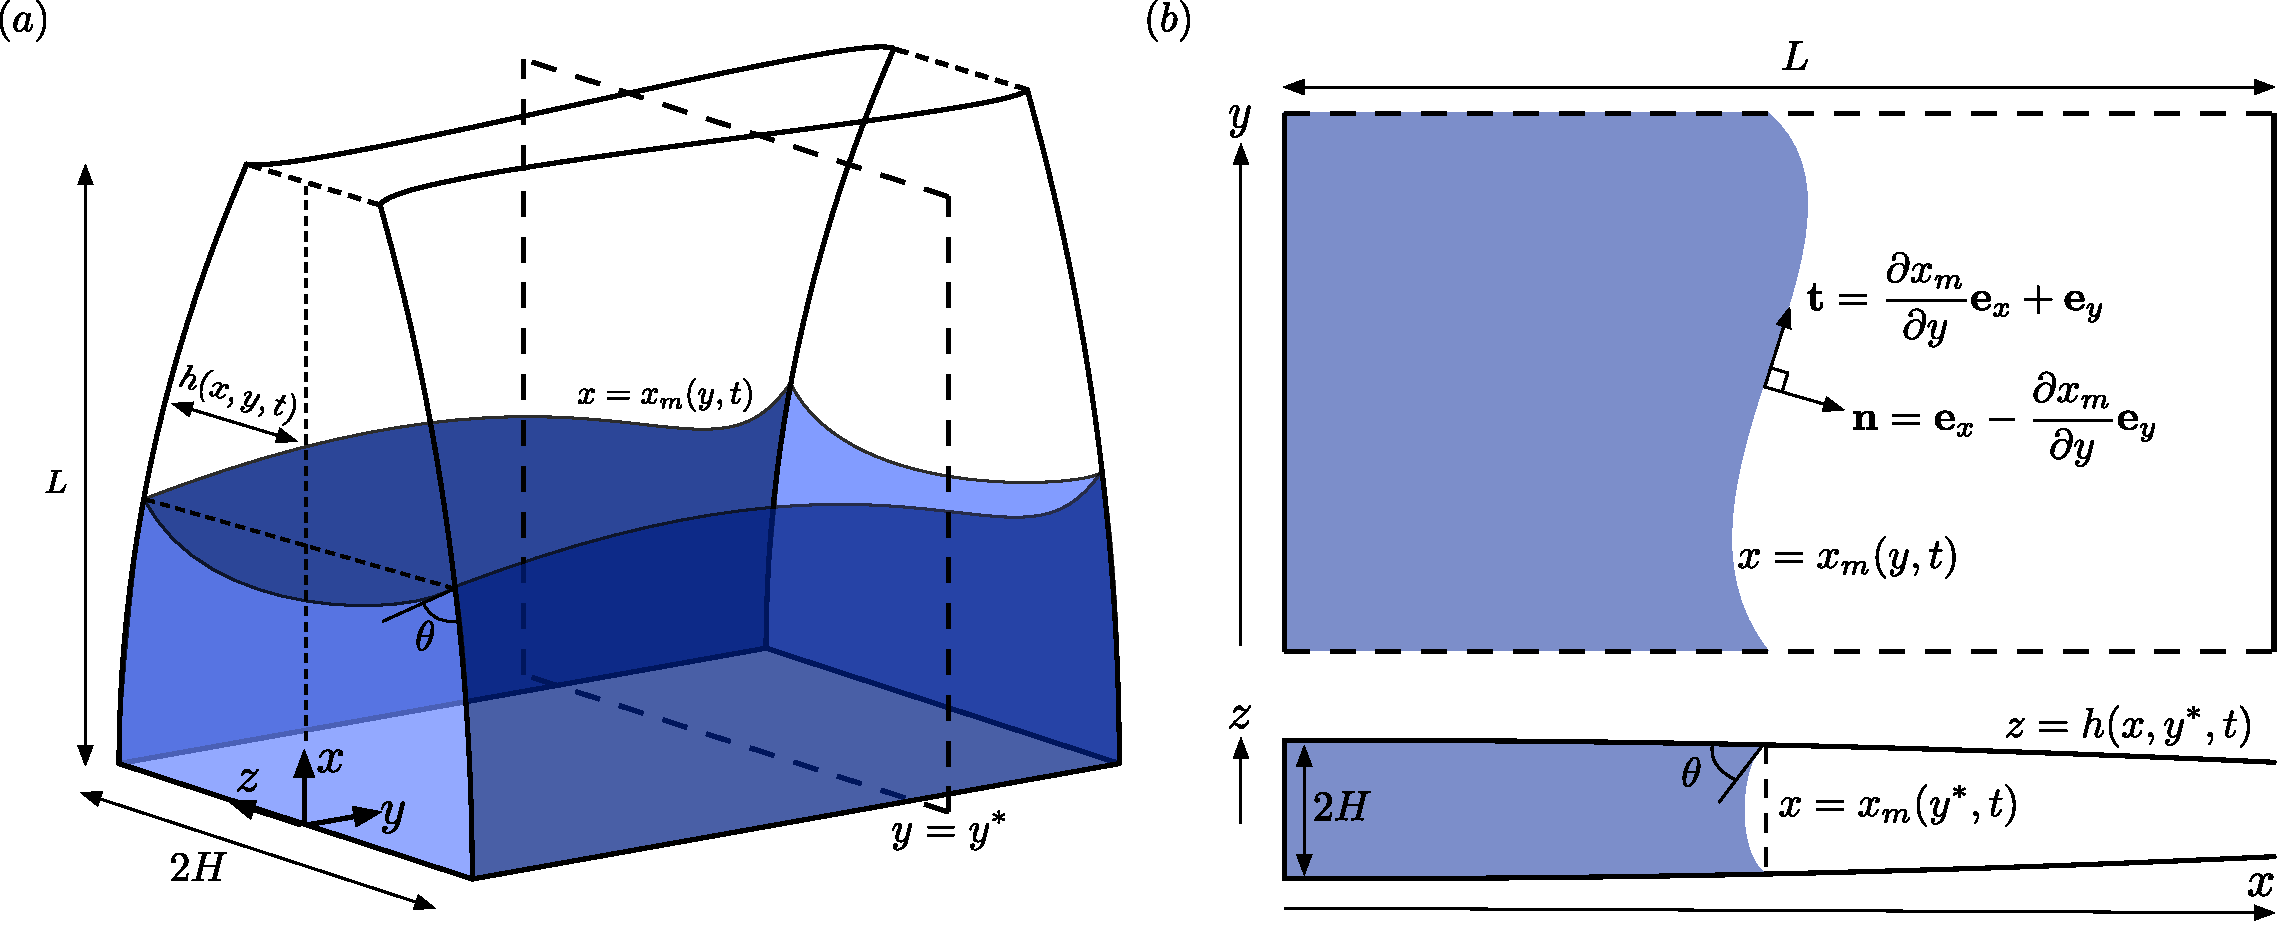
\includegraphics[scale=0.39]{Schematic_two_cross_sections}
\caption{(a) Schematic diagram of liquid in a narrow channel consisting of a solid base at $x =0$ and two deformable walls, whose midplanes are located at $z = \pm h(x,y,t)$. The liquid makes contact with the channel walls at $x = x_m(y,t)$. Note that the cell extends infinitely in the $y$-direction (only a section of which is shown). (b) Cross sections of the system shown in (a) in the $(x,y)$ plane (upper) and $(x,z)$ plane (lower); the latter is taken through $y = y^*$, indicated by the dashed box in (a).}
\label{fig:InstabilityChapter:Modelling:Schematic}
\end{figure}

\subsection{Preliminaries and assumptions}
We assume that the configuration is symmetric about $z = 0$ -- so we only need to consider a single channel wall -- and also that the walls are thin in comparison with their length, $b \ll L$. As a result, we can characterize the channel width at time $t > 0$ entirely by the position of the mid-plane of one wall~\citep{Reddy2006}, denoted by $h(x,y,t)$, (we shall therefore use `wall' and `wall mid-plane' interchangeably).
%We also assume that the channel walls are thin in comparison with the channel half-width, $b \ll H$, so it is reasonable to consider $2h(x,y,t)$ to be the width of the cavity between the walls.

The channel is wetted over a region $0 < x < x_m(y,t)$. We assume that $x_m \gg H$ throughout and also that variations in the flow in the $y$ direction occur on a length scale much longer than $H$, allowing us to use lubrication theory to model the liquid flow. The channel geometry does not provide a natural length scale for variations in the $y$-direction (as it does for the $x$-direction), but the length scale $L$ that we use in the horizontal direction is a natural choice. To ensure the lubrication approximation holds, we must ensure that the typical length scale of flow in the $y$-direction is much longer than $H$, but we shall check this a posteriori. With this assumption, the contact angle between liquid and solid is approximately that measured in the $(x,z)$ plane (Figure~\ref{fig:InstabilityChapter:Modelling:Schematic}(b)).

As in previous chapters, we neglect the weight and inertia of both the liquid and the channel walls, and the line force associated with surface tension.

%%%%%%%%%% Deleted Table %%%%%%%%%
%\renewcommand{\arraystretch}{1.2}
%\begin{table}[t]
%\begin{center}
%\begin{tabular}{ p{4cm} | p{3.5cm} | p{3cm}| p{2.5cm} }
%Neglected physics & In comparison with & Dimensionless no. & Value \\ \hline
%Droplet weight & Capillary forces & Bo = $\rho_l g H^2/\gamma$ & $10^{-5}$ \\
%Wall weight & Capillary forces & $\rho_s b g H/ \gamma$ & $10^{-3}$ \\
%Line force (surface tension) & Laplace Pressure & $\aspect = H/L$ & $10^{-4}$\\
%Droplet inertia & Viscosity & Re =  $\rho_l u_{\text{cap}} L/\mu$ & $10^{-2}$\\
%Wall inertia & Capillary forces & $\sqrt{\rho b L^3\gamma}/(\mu L)$ & $10^{-2}$\\
%Wall stretching & Wall bending & $b/L$ & $10^{-2}$
%\end{tabular}
%\end{center}

%\caption{\textcolor{red}{To be updated}NB: $u_{\text{cap}}$ is the capillary timescale from previous sections, $\mathcal{O}(10\mathrm{s})$. Beam inertia and capillarity calculations from comparing the timescale from beam inertia $T_{i} = \sqrt{IH_0/L^2 |\gamma \cos \theta|}$ and the capillary timescale of the flow $T_c = \mu L^2/ |\gamma \cos \theta|H_0$. $\sqrt{\rho b L^3\gamma}/(\mu L)\sim 10^{-3}$ using experimental values from chapter 3.  }\label{Table:Assumptions}
%\caption{Physical effects neglected in the mathematical model. Values in the final column are order of magnitude estimates from the experiments described in Chapter 3. Here, $u_{\text{cap}} = \gamma H/\mu L$ is the capillary velocity scale.}\label{Table:InstabilityChapter:Modelling:Assumptions}
%\end{table}
%%%%%%%%%% Deleted Table %%%%%%%%%



\subsection{Liquid flow}
Given the assumed small aspect ratio of the flow, we describe it using lubrication theory. The evolution of the pressure field $p(x,y,t)$ and the gap width are then coupled via Reynolds' equation
\begin{equation}\label{E:InstabilityChapter:Model:Liquid:Reynolds}
\ddp{h}{t} = \nabla.\left( \frac{h^3}{3\mu} \nabla p\right) \qquad \text{in}~0 < x < x_m(y,t).
\end{equation}

The free boundary of the liquid moves in response to the flux of fluid there and condensation of liquid onto it. Assuming that liquid condenses onto the interface at a uniform rate $C$ per unit area, the location of the interface evolves according to
\begin{equation}
\ddp{x_m}{t} = -\left.\frac{h^2}{3\mu}\nabla p .\frac{\mathbf{n}}{|\mathbf{n}|}\right|_{x = x_m(y,t)} + C
\end{equation}
where $\mathbf{n} = \mathbf{e}_x -\frac{\partial x_m}{\partial y}  \mathbf{e}_y$ is the normal to the interface in a plane at constant $z$ (Figure~\ref{fig:InstabilityChapter:Modelling:Schematic}(b)).

According to Laplace's law, the liquid pressure immediately beneath the interface is
\begin{equation}\label{E:InstabilityChapter:Model:Liquid:LaplaceBC}
 p(x = x_m, y,t) = \gamma\left(C_{\perp} + C_{\parallel}\right)
\end{equation}
where $C_{\perp}$ and $C_{\parallel}$ are the transverse and in-plane interfacial curvatures, respectively. Our neglect of gravity ensures that the meniscus is locally a circular arc in the $(x,z)$ plane (Figure~\ref{fig:InstabilityChapter:Modelling:Schematic}(b)), and hence
\begin{equation}\label{E:InstabilityChapter:Model:Liquid:CPerp}
C_{\perp} = -\frac{\cos \theta}{h(x=x_m,y,t)}.
\end{equation}

Our assumption that variations in the $y$-direction occur on a length scale much larger than $H$ means that we can approximate the in-plane interfacial curvature by
\begin{equation}\label{E:InstabilityChapter:Model:Liquid:CParallel}
C_{\parallel} = -\ddp{^2 x_m}{y^2}.
\end{equation}

We impose a no-flux condition at the rigid base,
\begin{equation}\label{E:InstabilityChapter:Model:Liquid:nofluxBC}
\ddp{p}{x}=0 \qquad \text{at}~x =0.
\end{equation}

\subsection{Wall deformation}
In the experiments shown in  Figure~\ref{fig:InstabilityChapter:Intro:ExptSnapshots}, the channel walls appear to undergo deformations that are large in comparison with their thickness.  We might expect, therefore, that the modelling of the channel's response to liquid pressure should include self-induced in-plane stretching~\citep{Timoshenko1959}. However, the energy penalty associated with in-plane stretching, which scales with $b/L$, is very high in comparison with the bending energy $(b/L)^3$ for thin flexible objects~\citep{Pini2016SciRep}. We therefore ignore stretching, and the channel walls can therefore be modelled as thin plates undergoing pure bending deformations under an applied load $q(x,y,t)$. The position of the channel wall mid-plane $h(x,y,t)$ therefore satisfies~\citep{Timoshenko1959}
\begin{equation}\label{E:InstabilityChapter:Model:Wall:Bilaplacian}
B\nabla^4 h = q.
\end{equation}

The channel deformation is coupled to the liquid pressure via the applied load:
\begin{equation}\label{E:InstabilityChapter:Model:Wall:BilaplacianPressure}
q(x,y,t) = \left\{\begin{array}{ll}  p(x,y,t) & 0 < x< x_m,\\ 0 & x_m < x < L
\end{array}\right.
\end{equation}

To close the problem, we require boundary conditions at the channel ends, $x= 0$ and $x = L$, as well as at the interface, $x = x_m$. We apply a straightforward clamped condition at $x = 0$,
\begin{equation}\label{E:InstabilityChapter:Model:Wall:ClampedBC}
h= H, \quad \ddp{h}{x} = 0 \qquad \text{at}~x = 0.
\end{equation}
The other boundary conditions require care, as they concern moments and shear forces. The wall supports bending moments
\begin{equation}\label{E:InstabilityChapter:Model:Wall:WallBendingMoments}
M_x = -B\left(\ddp{^2 h}{x^2} + \poisson \ddp{^2 h}{y^2}\right) \quad \text{and}\quad M_y = -B\left(\ddp{^2 h}{y^2} + \poisson \ddp{^2 h}{x^2}\right)
\end{equation}
parallel to the $x$- and $y$-axes, respectively, as well as a twisting moment
\begin{equation}\label{E:InstabilityChapter:Model:Wall:WallTwistingMoments}
M_{xy} = B(1-\poisson)\ddp{^2 h}{x \partial y}.
\end{equation}
Similarly, shear deformation can be decomposed into components $Q_x$ and $Q_y$ in directions parallel to the $x$- and $y$-axes, respectively. These are related to the channel wall position by
\begin{align}
Q_x &=  \ddp{M_x}{x} -\ddp{M_{xy}}{y} = -B \ddp{}{x} \left(\ddp{^2 h}{x^2} +\ddp{^2 h}{y^2}\right),\label{E:InstabilityChapter:Model:Wall:ShearX}\\
Q_y &= \ddp{M_{y}}{y} - \ddp{M_{xy}}{x} = -B \ddp{}{y} \left(\ddp{^2 h}{x^2} + \ddp{^2 h}{y^2}\right).\label{E:InstabilityChapter:Model:Wall:ShearY}
\end{align}
(See~\cite{Timoshenko1959}, for example, for a derivation of~\eqref{E:InstabilityChapter:Model:Wall:WallBendingMoments}--\eqref{E:InstabilityChapter:Model:Wall:ShearY}.)

We apply a free boundary condition at $x = L$:
\begin{equation}\label{E:InstabilityChapter:Model:Wall:FreeEndBC_all}
M_x = 0 = M_{xy} = Q_x \quad \text{at}~x = L.
\end{equation}
For a thin plate undergoing purely bending deformations, however, the three boundary conditions~\eqref{E:InstabilityChapter:Model:Wall:FreeEndBC_all} are too many, and were demonstrated by~\cite{Tait1883} to be equivalent to the two boundary conditions~\citep{Timoshenko1959},
\begin{equation}\label{E:InstabilityChapter:Model:Wall:FreeEndBC}
\ddp{^2 h}{x^2} + \poisson \ddp{^2 h}{y^2} = 0 = \ddp{^3 h}{x^3} + (2-\poisson) \ddp{^3 h}{x \partial y^2}\quad \text{at}~x = L.
\end{equation}
%\red{Does this need more explanation? (p84 of Plates and Shells)}

%Comment on the presence of y derivatives meaning we can't integrate out the dry region, in general?
The free boundary condition~\eqref{E:InstabilityChapter:Model:Wall:FreeEndBC} applies only when the channel walls do not touch. If deformations become large enough for contact,~\eqref{E:InstabilityChapter:Model:Wall:FreeEndBC} must be modified but here we focus on early times when only a small amount of liquid is present and the associated deformations are small.

At the meniscus, we assume that the channel and its slope, as well as the moments and shear forces it supports are continuous:
\begin{align}\label{E:InstabilityChapter:Model:Wall:ContinuityBC}
\left[ h \right]\jump{x_m}  =  \left[\ddp{h}{x} \right]\jump{x_m} = \left[\ddp{h}{y} \right]\jump{x_m} &=0 \\ \left[M_x \right]\jump{x_m} =   \left[M_y \right]\jump{x_m} =  \left[M_{xy} \right]\jump{x_m} =  \left[Q_x \right]\jump{x_m} =  \left[Q_y \right]\jump{x_m} &=0.
\end{align}
Here $\left[ f \right]\jump{\chi} = f(\chi+,y,t) - f(\chi-,y,t)$ denotes the change across the $x = \chi$, and has both $y$ and $t$-dependence in general. (In contrast to previous chapters, here we explicitly state where the jump condition is being applied.)

\subsection{Non-dimensionalization}\label{S:InstabilityChapter:Modelling:NonDim}
Variations in the $x$- and $z$-directions have natural length scales set by the channel geometry, and corresponding dimensionless variables (denoted by hats)
\begin{equation}\label{E:InstabilityChapter:Modelling:NonDim:SpatialScaling}
\hat{h} = \frac{h}{H}, \qquad \hat{x} = \frac{x}{L}, \qquad \hat{x}_m = \frac{x_m}{L}.
\end{equation}

The channel geometry does not provide a length scale for variations in the $y$-direction, and so we choose the scale $L$ used in the $x$-direction, introducing
\begin{equation}\label{E:InstabilityChapter:Modelling:NonDim:yscaling}
\hat{y} = \frac{y}{L}.
\end{equation}
Note that in the scaling argument of \S\ref{S:InstabilityChapter:Scaling}, we identified a critical wavelength for instability in the $y$-direction:
\begin{equation}\label{E:InstabilityChapter:Modelling:NonDim:LengthscaleFromScaling}
L_y = \left(\frac{B H^3}{\gamma  \cos^2 \theta L^3}\right)^{1/2},
\end{equation}
and so we anticipate the appearance of the dimensionless wavenumber
\begin{equation}\label{E:InstabilityChapter:Modelling:NonDim:ExpectedWavenumber}
L/L_y =  \left(\frac{\gamma \cos^2 \theta L^5}{B H^3}\right)^{1/2}
\end{equation}
in our stability analysis.

As elsewhere in this thesis, dimensionless time and pressure variables are introduced by scaling with a capillary time scale and a bending pressure scale, respectively,
\begin{equation}\label{E:InstabilityChapter:Modelling:NonDim:TimeAndPressureScaling}
\hat{t} =\frac{t}{ \tau_c} =  \frac{|\gamma \cos \theta| H}{\mu L^2}t, \qquad \hat{p} = \frac{L^4}{B}p.
\end{equation}

After scaling variables in this way, and combining Reynolds' equation~\eqref{E:InstabilityChapter:Model:Liquid:Reynolds} with the bending equation~\eqref{E:InstabilityChapter:Model:Wall:Bilaplacian}--\eqref{E:InstabilityChapter:Model:Wall:BilaplacianPressure}, we obtain the following system of equations:
\begin{align}
\ddp{\hat{h}}{\hat{t}} &=\frac{1}{3|\nu|}\hat{\nabla}. \left[\hat{h}^3\hat{\nabla}\hat{p}  \right] & & 0 <  \hat{x} < \hat{x}_m(\hat{y},\hat{t}),\label{E:InstabilityChapter:Modelling:NonDim:PDE1}\\
  \hat{p}&=0 & &
\hat{x}_m(\hat{y},\hat{t}) < \hat{x} < 1,\label{E:InstabilityChapter:Modelling:NonDim:PDE2}\\
\hat{p} &=\hat{\nabla}^4 \hat{h}& &0 < \hat{x} < 1,\label{E:InstabilityChapter:Modelling:NonDim:PDE3}
\end{align}
where
\begin{equation}\label{E:InstabilityChapter:Modelling:NonDim:Bendability}
\bendability = \frac{\gamma \cos \theta L^4}{B H^2}
\end{equation}
is the familiar channel bendability.

The dimensionless boundary conditions on the channel wall position (equations~\eqref{E:InstabilityChapter:Model:Wall:ClampedBC}, \eqref{E:InstabilityChapter:Model:Wall:FreeEndBC} and~\eqref{E:InstabilityChapter:Model:Wall:ContinuityBC}) are
\begin{equation}\label{E:InstabilityChapter:Modelling:NonDim:ClampedBC}
\hat{h} = 1, \quad \ddp{\hat{h}}{\hat{x}} = 0 \quad \text{at}~ \hat{x} = 0,
\end{equation}
\begin{equation}\label{E:InstabilityChapter:Modelling:NonDim:FreeBC}
\ddp{^2 \hat{h}}{ \hat{x}^2}  + \poisson \ddp{^2 \hat{h}}{\hat{x}^2} =  \ddp{^3 \hat{h}}{ \hat{x} ^3}  + (2-\poisson) \ddp{^3 \hat{h}}{\hat{x}\partial \y^2}=0 \quad \text{at}~ \hat{x} = 1,
\end{equation}
\begin{align}\label{E:InstabilityChapter:Modelling:NonDim:ContinuityBC1}
0 & =\left[ \hat{h} \right]_{x_m^-}^{x_m^+} = \left[\ddp{\hat{h}}{\hat{x}}\right] _{x_m^-}^{x_m^+}  = \left[\ddp{\hat{h}}{\hat{y}} \right]_{x_m^-}^{x_m^+}  ,\\
0 &=  \left[\ddp{^2 \hat{h}}{\hat{x}^2} +\poisson \ddp{^2 \hat{h}}{\hat{y}^2}  \right]_{x_m^-}^{x_m^+} = \left[\ddp{^2 \hat{h}}{\hat{y}^2} +\poisson \ddp{^2 \hat{h}}{\hat{x}^2}  \right]_{x_m^-}^{x_m^+}  = \left[\ddp{^2 \hat{h}}{\hat{x} \partial \hat{y}}  \right]_{x_m^-}^{x_m^+}  \label{E:InstabilityChapter:Modelling:NonDim:ContinuityBC2}
\\
0& = \left[\ddp{}{\hat{x}} \left(\ddp{^2 \hat{h}}{\hat{x}^2} + \ddp{^2 \hat{h}}{\hat{y} ^2}\right) \right]_{x_m^-}^{x_m^+}  = \left[\ddp{}{\hat{y}} \left(\ddp{^2 \hat{h}}{\hat{x}^2} + \ddp{^2 \hat{h}}{\hat{y} ^2}\right) \right]_{x_m^-}^{x_m^+}  .
\end{align}
The boundary conditions on the pressure (equations~\eqref{E:InstabilityChapter:Model:Liquid:LaplaceBC} and~\eqref{E:InstabilityChapter:Model:Liquid:nofluxBC}) become
\abeqn{E:InstabilityChapter:Modelling:NonDim:PressureJumpBC}{
\ddp{\hat{p}}{x} = 0 \quad \text{at}~\hat{x} = 0, \qquad \quad \hat{p} = -\nu\left(\frac{1}{\hat{h}} + \aspect \ddp{^2 \hat{x}_m}{\hat{y}^2}\right)\quad \text{at}~\hat{x} = \hat{x}_m.}
Here, the aspect ratio $\aspect = H/(L \cos \theta)$ arises as the ratio between the typical radii of curvature in the transverse and in-plane directions. Note that the sign of $\aspect$ reflects the wetting conditions:  $\aspect >0$ for wetting conditions ($\theta < 90\si{\degree}$) and $\nu$:   $\aspect <0$ for non-wetting conditions ($\theta > 90\si{\degree}$); the sign of $\aspect$ is always the same as the sign of $\nu$, so their ratio $\nu/\aspect >0$.

We retain the final term in~\eqref{E:InstabilityChapter:Modelling:NonDim:PressureJumpBC} despite being higher order in $\aspect \ll 1$ (we assume $\cos \theta \sim \mathcal{O}(1)$); for periodic perturbations with wavenumber $k$, this term is $\mathcal{O}(\aspect k^2)$ and will become important for large wavenumber (short wavelength) perturbations. (Note also that the final term in~\eqref{E:InstabilityChapter:Modelling:NonDim:PressureJumpBC} is larger than the errors introduced by using lubrication theory, which are $\mathcal{O}(\aspect^2)$.)

The dimensionless meniscus position $\hat{x}_m = \hat{x}_m(\hat{y}, \hat{t})$ evolves according to
\begin{equation}\label{E:InstabilityChapter:Modelling:NonDim:Kinematic}
\ddp{ \hat{x} _m}{\hat{t}} = -\left.\frac{\hat{h}^2}{3|\nu|}\left(\ddp{\hat{p}}{\hat{x}} - \ddp{\hat{x}_m}{\hat{y}}\ddp{\hat{p}}{\hat{y}} \right)  \right|_{\hat{x} = \hat{x}_m} +  \hat{C},
\end{equation}
correct to $\mathcal{O}(\aspect^2)$, where $\hat{C} = C/U_\text{fill}$ describes the speed of meniscus motion caused by condensation relative to the capillary filling speed $U_\text{fill} = L/\tau_{c}$.

We now move on to consider the quasi-static base state and its stability. We shall henceforth drop hats (including on the condensation rate $\hat{C}$); all variables are dimensionless unless otherwise stated.

\section{No condensation}\label{S:InstabilityChapter:SlowCondensation}
\renewcommand{\varepsilon}{\delta} %rename the size of the perturbation to agree with the scaling argument
\newcommand{\param}{\xi} %ratio of bending energies (for use in the asymptotics)
We consider first the case of no condensation, $C = 0$, so that we can isolate the competing curvature instability from the effect of condensation driven dynamics and a changing amount of liquid in the channel

\subsection{Equilibria}\label{S:InstabilityChapter:BaseState:Equilibria}
%meniscus position in full problem xm, here x0
With $C = 0$, solutions of the steady form of the model equations equations~\eqref{E:InstabilityChapter:Modelling:NonDim:PDE1}--\eqref{E:InstabilityChapter:Modelling:NonDim:Kinematic} may exist.

These equilibria are uniform in the $y$-direction with meniscus position $x_m = x_0$ and channel shape $h_e(x)$ (we suppress the $y$-dependence to reflect uniformity in this direction). These equilibria were studied in detail by~\cite{Taroni2012JFM}, who used the meniscus position, $x_0$, to parametrize the wall shapes and the cross sectional volume,
\begin{equation}
V  = V(x_0) = \int_{0}^{x_0} h_e(x)~\mathrm{d}x.
\end{equation}
Taroni and Vella showed that the equilibria then have wall shapes
\begin{equation}\label{E:InstabilityChapter:FlatInterface:NoCond:EqShape}
\h_e(\x) = \left\{\begin{array}{l l}
 \h_m+ \frac{\nu}{24 \h_m}\left[4 x_0^3( \x_0 - \x) - ( \x_0 - \x)^4\right] &  0 < \x <  \x_0, \\
 \h_m -\frac{\nu }{6 h_m}(\x - \x_0) \x_0^3 & \x_0 < \x < 1,
\end{array}\right.
\end{equation}
with associated uniform pressure $p = p_0 = -\nu/h_m$. Here $h_m \coloneqq  \h_e(\x_0)$ and $x_0$ must satisfy
\abeqn{E:InstabilityChapter:FlatInterface:NoCond:MeniscusDispQuadratic}{
\h_m^2 - \h_m + \frac{\nu \x_0^4 }{8} = 0, \quad \text{and}\quad V= \x_0 \h_m + \frac{3\nu }{40 \h_m x_0^5}.
}
In addition, to avoid situations in which the walls touch, we require
\begin{equation}\label{E:InstabilityChapter:FlatInterface:NoCond:NoTouchCond}
\h_e(\x = 1) = \h_m - \frac{\nu  (1- \x_0 )\x_0^3}{6 \h_m} > 0.
\end{equation}

Note that equation~\eqref{E:InstabilityChapter:FlatInterface:NoCond:MeniscusDispQuadratic}a has roots
\begin{equation}\label{E:InstabilityChapter:FlatInterface:NoCond:MeniscusWidth}
h_m = h_m^{\pm} = \frac{1}{2}\left[ 1 \pm \left(1 - \frac{\nu x_0^4}{2}\right)^{1/2}\right],
\end{equation}
so two equilibria at the same parameter pair $(\nu , V)$ may exist. We distinguish between the two equilibria by referring to them as `$+$' and `$-$' roots according to the sign taken in~\eqref{E:InstabilityChapter:FlatInterface:NoCond:MeniscusWidth}.

\begin{figure}[t]
\centering
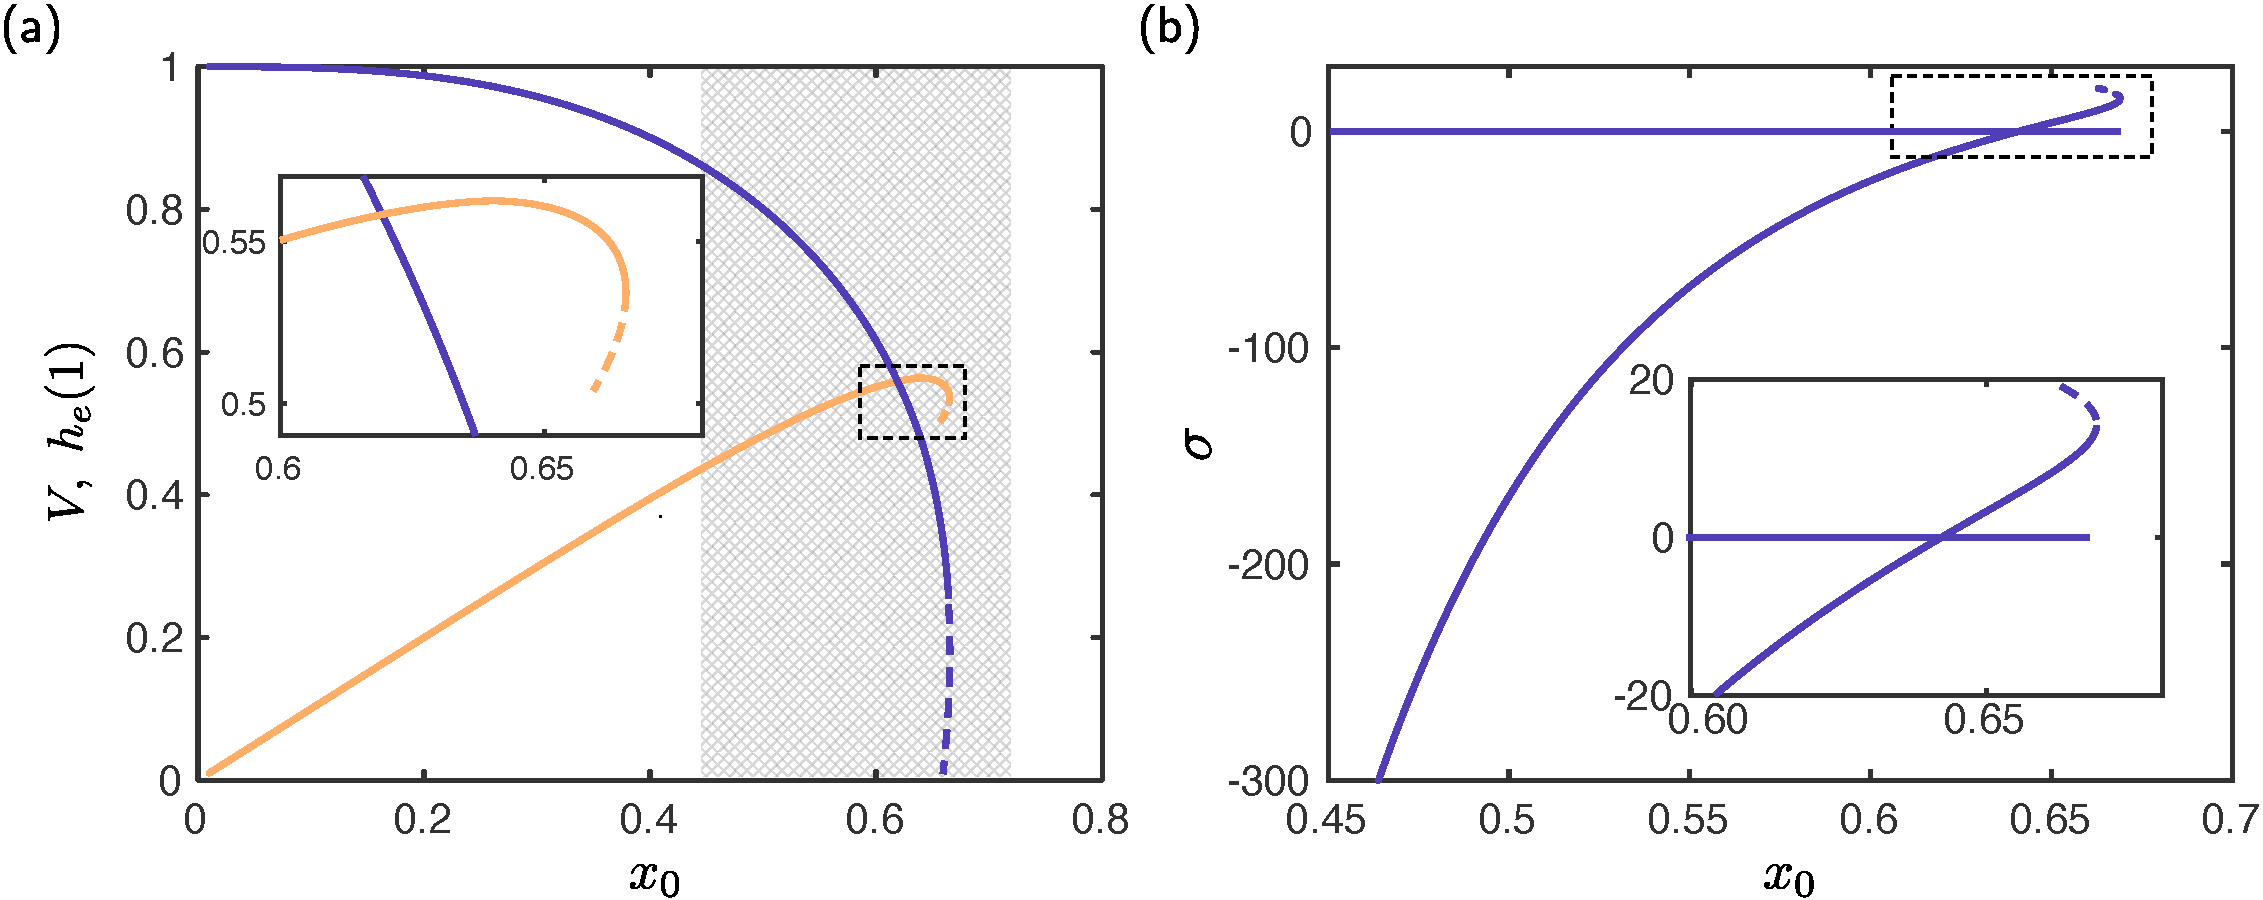
\includegraphics[width =0.98\textwidth]{tv12_stability_nu_is_10_by_x0}
\caption{(a) Equilibrium volume  $V$ (orange curve) and free end channel width $h_e(x = 1)$ (purple curve) in steady solutions of the model equations~\eqref{E:InstabilityChapter:Modelling:NonDim:PDE1}--\eqref{E:InstabilityChapter:Modelling:NonDim:Kinematic} with $\nu = 10$. The solid and dashed parts of the curve corresponds to the `$+$' and `$-$' roots of~\eqref{E:InstabilityChapter:FlatInterface:NoCond:MeniscusWidth}, respectively. Inset: a close up of the section of the main figure indicated by the black dashed box, in which multiple equilibria with the same meniscus position exist. (b) Growth rate $\sigma_u$ of uniform perturbations (i.e.~of the form~\eqref{E:InstabilityChapter:FlatInterface:NoCond:uniform_perturbation}) to the equilibria indicated by the points in (a) that lie within the hatched box. Each equilibria is associated with two values of $\sigma_u$, one of which is always zero. Inset: a close up of the section of the main figure indicated by the black dashed box.}\label{fig:InstabilityChapter:FlatInterface:NoCond:Tv12_analogue}
\end{figure}

The `$-$' root exists only for small band of sufficiently large meniscus position $x_0$ (or, equivalently, for sufficiently large $V$, see Figure~\ref{fig:InstabilityChapter:FlatInterface:NoCond:Tv12_analogue}(a)) (the `$-$' root violates the no-touching condition~\eqref{E:InstabilityChapter:FlatInterface:NoCond:NoTouchCond} for smaller $x_0$), whilst the `$+$' root exists for a large range of $x_0$ including $0$.  Further, the `$+$' root is associated with smaller deformations; in particular, if
\begin{equation}\label{E:InstabilityChapter:FlatInterface:NoCond:epsilon_def}
\epsilon \coloneqq |\nu| V^4 \ll 1,
\end{equation}
then from~\eqref{E:InstabilityChapter:FlatInterface:NoCond:MeniscusDispQuadratic}, we find that $h_m^+ = 1 + \mathcal{O}(\epsilon)$, whilst $h_m^- = \mathcal{O}(\epsilon)$. If we take the $`+'$ root in this small deformation case, then from~\eqref{E:InstabilityChapter:FlatInterface:NoCond:MeniscusDispQuadratic} we find that the meniscus position satisfies
\begin{equation}\label{E:InstabilityChapter:FlatInterface:NoCond:Asymptotic_x0_to_V}
 x_0 = V\left[1 + \frac{\mathrm{sgn}(\nu)\epsilon}{20}  + \mathcal{O}(\epsilon^2)\right],
\end{equation}
where $\mathrm{sgn}$ is the signum function. The associated channel shape is
\begin{equation}\label{E:InstabilityChapter:FlatInterface:NoCond:Asymptotic_channel_shape}
h_e(x) = 1 + \mathrm{sgn}(\nu)\epsilon\psi \left(\frac{x}{V}\right) + \mathcal{O}(\epsilon^2),\qquad \psi(s) = \frac{-1}{8} + \frac{1}{24}\left[4(1-s) - (1-s)^4\right].
\end{equation} Equation~\eqref{E:InstabilityChapter:FlatInterface:NoCond:Asymptotic_x0_to_V} demonstrates that the meniscus position and the volume are approximately equal when deformations are small, which is encoded by~\eqref{E:InstabilityChapter:FlatInterface:NoCond:epsilon_def}. Expressions~\eqref{E:InstabilityChapter:FlatInterface:NoCond:Asymptotic_x0_to_V} and~\eqref{E:InstabilityChapter:FlatInterface:NoCond:Asymptotic_channel_shape} will be important when we formally consider the case of small deformations in due course.

Before moving on to consider the stability of these equilibria to in-plane perturbations, we briefly consider their stability to \textit{uniform} perturbations (or, equivalently to in-plane perturbations with zero wavenumber). In this scenario, the instability mechanism is somewhat simpler than that described in \S\ref{S:InstabilityChapter:Mechanism:Elasticity}: the meniscus would like to advance to wet the beams over a longer length, but the additional deformation that results will incur a bending energy penalty.

Following Taroni and Vella, we probe the stability of the equilibria by substituting
\begin{equation}\label{E:InstabilityChapter:FlatInterface:NoCond:uniform_perturbation}
h = h_e(x) + \varepsilon \Lambda_0(x)\exp(\sigma_u t),~p = p_0 + \varepsilon \Pi_0(x)\exp(\sigma_u t),~ x_0 = x_0 +  \varepsilon \exp(\sigma_u t),
\end{equation}
where $\varepsilon \ll 1$ is arbitrary, into the model equations~\eqref{E:InstabilityChapter:Modelling:NonDim:ClampedBC}--\eqref{E:InstabilityChapter:Modelling:NonDim:Kinematic}; linearizing in $\varepsilon$ yields a boundary value problem which can be solved numerically to obtain the growth rate $\sigma_u$ for a given $\nu$ and $V$ (the numerical procedure is described in following section for in-plane perturbations of any wavenumber).

For each of the roots of~\eqref{E:InstabilityChapter:FlatInterface:NoCond:MeniscusWidth}, this boundary value problem has two solutions, resulting in two unique values of $\sigma_u$ for each equilibrium (Figure~\ref{fig:InstabilityChapter:FlatInterface:NoCond:Tv12_analogue}(b)). One of these growth rates, $\sigma_u^2$, is always zero; the corresponding solution does not conserve mass -- it refers to a uniform advance of the meniscus with no corresponding change in channel shape.

The second of these growth rates, $\sigma_u^1$, is negative and large in magnitude for small $x_0$ (Figure~\ref{fig:InstabilityChapter:FlatInterface:NoCond:Tv12_analogue}(b)). Increasing $x_0$ is accompanied by an increase in $\sigma_u^1$ because  the bending penalty incurred by the perturbation is reduced when the meniscus is closer to the free end, when the channel is effectively softer. For a small range of $x_0$, the equilibrium corresponding to the `$+$' root in~\eqref{E:InstabilityChapter:FlatInterface:NoCond:MeniscusWidth} are unstable (the growth of perturbations is positive), whilst those corresponding to the `$-$' root are always unstable.

As we a primarily interested in low volume configurations, we shall henceforth ignore the equilibria corresponding to the `$-$' root in~\eqref{E:InstabilityChapter:FlatInterface:NoCond:MeniscusWidth}.


\subsection{Periodic perturbations}\label{S:InstabilityChapter:SlowCondensation:PeriodicPerturbations}
\renewcommand{\Lambda}{H}
\renewcommand{\Pi}{P}
To analyze the linear stability of these equilibria to perturbations with an in-plane component, we let
\begin{align}
h &= h_e(x) + \varepsilon \Lambda(x)\exp(\sigma t + i k y),\label{E:InstabilityChapter:SlowCondensation:Periodic:Perturbation1} \\
 p &= p_m + \varepsilon \Pi(x)\exp(\sigma t + i k y),\\ x_m  &= x_0 +  \varepsilon \exp(\sigma t + i k y),\label{E:InstabilityChapter:SlowCondensation:Periodic:Perturbation3}
\end{align}
with $\varepsilon$ again arbitrary. Substituting~\eqref{E:InstabilityChapter:SlowCondensation:Periodic:Perturbation1}--\eqref{E:InstabilityChapter:SlowCondensation:Periodic:Perturbation3} into the model equations~\eqref{E:InstabilityChapter:Modelling:NonDim:ClampedBC}--\eqref{E:InstabilityChapter:Modelling:NonDim:Kinematic} (with $C = 0$) and linearizing yields a coupled boundary value problem (BVP) for $\Lambda$ and $\Pi$:

\begin{align}
\sigma \Lambda &=  \frac{h_e^2}{3|\nu|}\left[3\dd{h_e}{x} \dd{\Pi}{x} + h_e\left(\dd{^2 \Pi}{x^2} - k^2 \Pi\right)\right] & &0 < x < x_0,\label{E:InstabilityChapter:SlowCondensation:Periodic:ODEwet}\\
0 &= \Pi & &x_0 < x < 1,\label{E:InstabilityChapter:SlowCondensation:Periodic:ODEdry}\\
\Pi &= \dd{^4 \Lambda}{x^4} - 2k^2 \dd{^2 \Lambda}{x^2} + k^4 \Lambda & & 0 < x <1.\label{E:InstabilityChapter:SlowCondensation:Periodic:pressure2shape}
\end{align}
The boundary conditions on~\eqref{E:InstabilityChapter:SlowCondensation:Periodic:ODEwet}--\eqref{E:InstabilityChapter:SlowCondensation:Periodic:pressure2shape} are
\begin{align}
\Lambda &= 0 = \dd{\Lambda}{x} = \dd{\Pi}{x} & &\text{at}~x = 0,\label{E:InstabilityChapter:SlowCondensation:Periodic:BC_at_0}\\
\Pi &= \frac{\nu}{h_m^2}\left(\dd{h_e}{x} + \Lambda\right) + \nu \aspect k^2 & &\text{at}~x = x_0,\label{E:InstabilityChapter:SlowCondensation:Periodic:pressure_bc}\\
\dd{^2 \Lambda}{x^2} - \poisson k^2
\Lambda &= 0 = \dd{^3 \Lambda}{x^3} - (2-\poisson)k^2 \dd{\Lambda}{x} & &\text{at}~x = 1,\label{E:InstabilityChapter:SlowCondensation:Periodic:BC_at_1}
\end{align}
\begin{equation}\label{E:InstabilityChapter:SlowCondensation:Periodic:jump_conds}
\left[\Lambda\right]\jump{x_0}= \left[\dd{\Lambda}{x}\right]\jump{x_0} = \left[\dd{^2\Lambda}{x^2}\right]\jump{x_0}= 0, \quad\left[\dd{^3 \Lambda}{x^3}\right]\jump{x_0} = \frac{\nu}{h_m },
\end{equation}
The growth rate $\sigma$ satisfies
\begin{equation}\label{E:InstabilityChapter:SlowCondensation:Periodic:kinematic}
\sigma = -\frac{h_m^2}{3|\nu|}\left.\ddp{\Pi}{x}\right|_{x = x_0}.
\end{equation}

The terms on the right hand side of~\eqref{E:InstabilityChapter:SlowCondensation:Periodic:pressure_bc} elucidate the mechanism described in \S\ref{S:InstabilityChapter:Mechanism:Elasticity}; in order, they correspond to the transverse curvature changes arising from channel tapering set by the base state, transverse changes arising from the elastic response to the perturbation, and the stabilizing in-plane curvature of the perturbation. 

\subsubsection{Numerical results}\label{S:InstabilityChapter:NoCond:Numerics}
To solve the BVP numerically, we first write it as a first order system of ODEs; we solve this system using the BVP4C routine implemented in \textsc{matlab}~\citep{Kierzenka2001BVP}.
As for the uniform perturbation discussed in the previous section, the problem has two solutions and which is of these is returned depends on the proximity to the initial guess for $\sigma$. The corresponding growth rates $\sigma_i, i = 1,2$ originate from $\sigma_u^i$ (i.e.~$\sigma_i(k= 0) = \sigma_u^i$). In particular, those solutions on the $\sigma_2$ branch originate from the solution that does not conserve mass, so would need mass adding; with $k \neq 0$, however, it is possible to move mass in the $y$-direction.

It is the $\sigma_2$ that is of most interest here: this branch shows positive growth rates (Figure~\ref{fig:InstabilityChapter:SlowCondensation:GrowthRates}(a)); the branch originating at $\sigma_u^1$ has very high decay rates even for small $k$. To reflect this, we drop the index and take $\sigma =  \sigma_2$ henceforth.

%Generic features: growth rate positive for sufficiently small $\khat$, and $h_1(x_0) < 0$
Dispersion relations $\sigma(k)$ are obtained by solving the BVP~\eqref{E:InstabilityChapter:SlowCondensation:Periodic:ODEwet}--\eqref{E:InstabilityChapter:SlowCondensation:Periodic:kinematic} numerically over a range of different $k$ values, and are shown in Figure~\ref{fig:InstabilityChapter:SlowCondensation:GrowthRates} for different cross sectional volumes $V = V(x_0)$. We see that $\sigma > 0$ for sufficiently small wavenumbers -- an observation that is generic in numerical solutions of the BVP. In addition, $\sigma\sim k^2$ as $k \to 0$ (Figure~\ref{fig:InstabilityChapter:SlowCondensation:GrowthRates}(b)) as suggested by the scaling argument~\eqref{E:InstabilityChapter:Scaling:amplitude_ode}. (We shall derive this formally in the case of small deformations shortly.)

\begin{figure}[t]
\centering
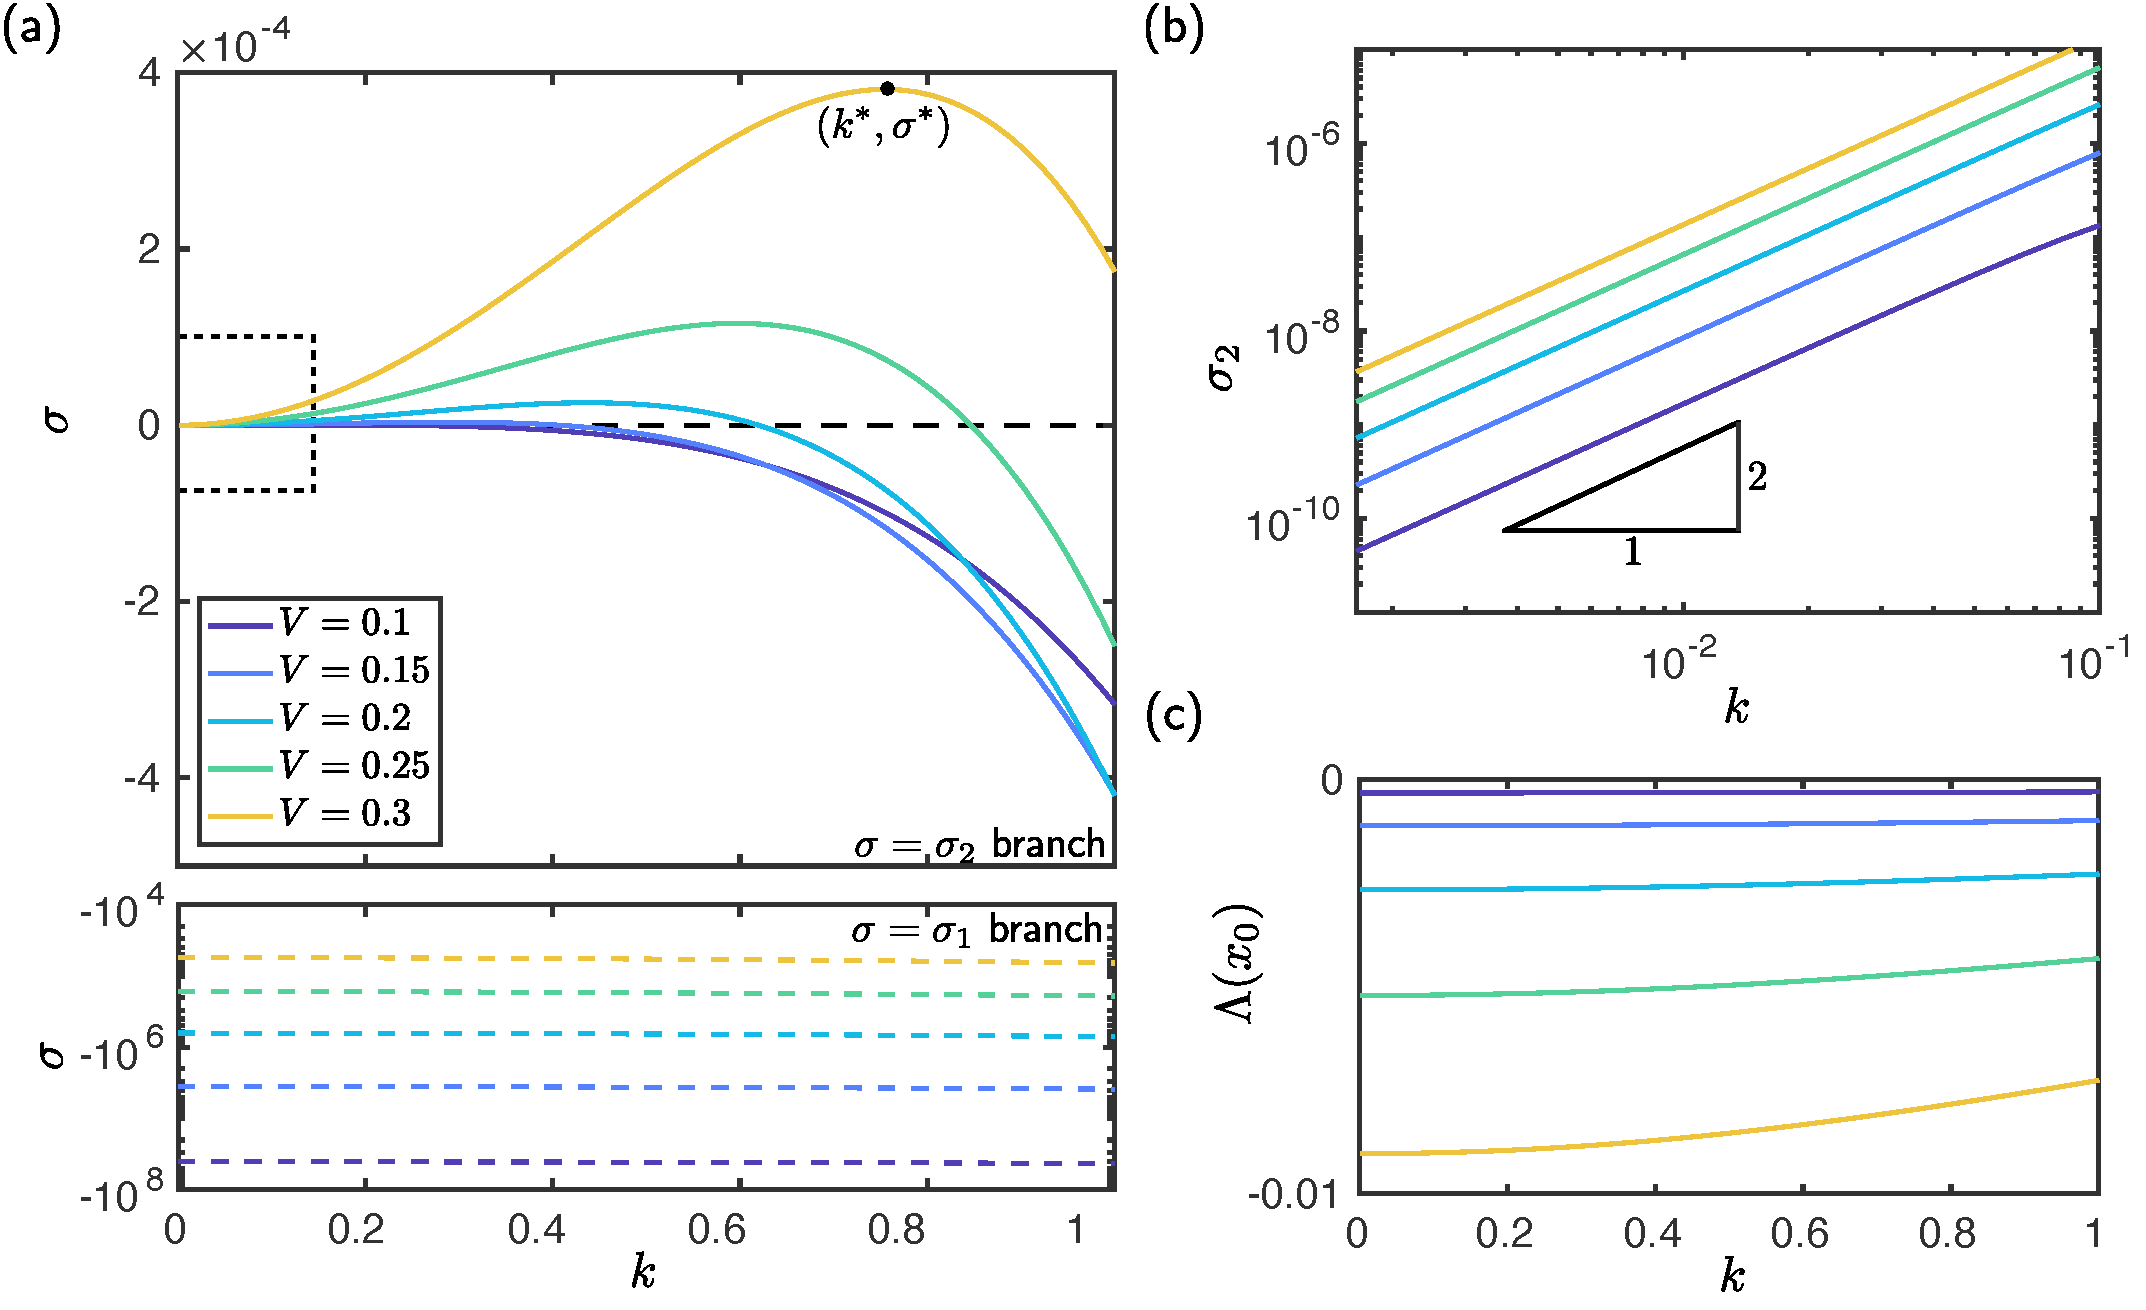
\includegraphics[width = 0.98\textwidth]{Growth_rates}
\caption{Numerical solutions of the boundary value problem arising from periodic perturbations with wavenumber $k$ to an equilibrium with cross-sectional volume $V$ (values indicated by the legend), $\nu = 1$ and $\aspect = 0.01$. (a) Growth rates $\sigma_{i}, i = 1,2$ of the perturbation shown as solid ($i = 1$) and dashed ($i = 2$) lines. The black dashed line indicates $\sigma = 0$. Note that the bottom axis uses a semi-logarithmic scale to allow all the data to be seen. (b) Zoom in on the small $k$ region of the $\sigma_1$ curve in the dashed box in (a), plotted on logarithmic axes. (c) Value of shape perturbation at the interface. Colours are as in (a) and (b).}
\label{fig:InstabilityChapter:SlowCondensation:GrowthRates}
\end{figure}


Another generic feature of numerical solutions of the BVP is that the perturbation to the shape is negative at the meniscus, $\Lambda(x_0) <0$  (Figure~\ref{fig:InstabilityChapter:SlowCondensation:GrowthRates}(c)): the channel deformation of the base state is enhanced at protrusions and reduced at invaginations. (For non-wetting configurations with $\nu <0$, $\Lambda(x_0)$ is positive, again corresponding to enhanced deformation at protrusions.)

For the parameter values used in Figure~\ref{fig:InstabilityChapter:SlowCondensation:GrowthRates}, the fastest growing mode, denoted $k^*$, and the corresponding growth rate $\sigma^* = \sigma(k^*)$, both increase with cross-sectional volume $V$. This is in qualitative agreement with the scaling argument~\eqref{E:InstabilityChapter:Scaling:SigmaScaling1}, which, after non-dimensionalizing with the length scale $L$ and time scale $\tau_c$, suggests the typical scales
\begin{equation}\label{E:InstabilityChapter:SlowCondensation:NumericalSols:DimensionlessScalings}
k_c  = \left(\frac{\nu V^3}{a}\right)^{1/2}, \qquad \sigma_c = \frac{\nu^2 V^7}{|a|}.
\end{equation}

For a quantitative assessment of the scaling argument, we rescale the numerically obtained dispersion relations $\sigma(k)$ according to~\eqref{E:InstabilityChapter:SlowCondensation:NumericalSols:DimensionlessScalings} (Figure~\ref{fig:InstabilityChapter:SlowCondensation:CollapsedGrowthRates}(a)). Here we see that the data collapse onto a universal curve for $\nu \ll 1$ (indicated by dark shades in Figure~\ref{fig:InstabilityChapter:SlowCondensation:CollapsedGrowthRates}(a)), but deviate when $\nu \gg 1$ (light shades). In addition, the deviation occurs sooner (i.e. at lower $\nu$ values) for larger volume $V$ where the base state deformation is expected to be larger. To predict the envelope enclosing the curves $\sigma/\sigma_c$ we now perform an asymptotic expansion of the BVP~\eqref{E:InstabilityChapter:SlowCondensation:Periodic:ODEwet}--\eqref{E:InstabilityChapter:SlowCondensation:Periodic:kinematic} in the limit of small deformations.

\begin{figure}[t]
\centering
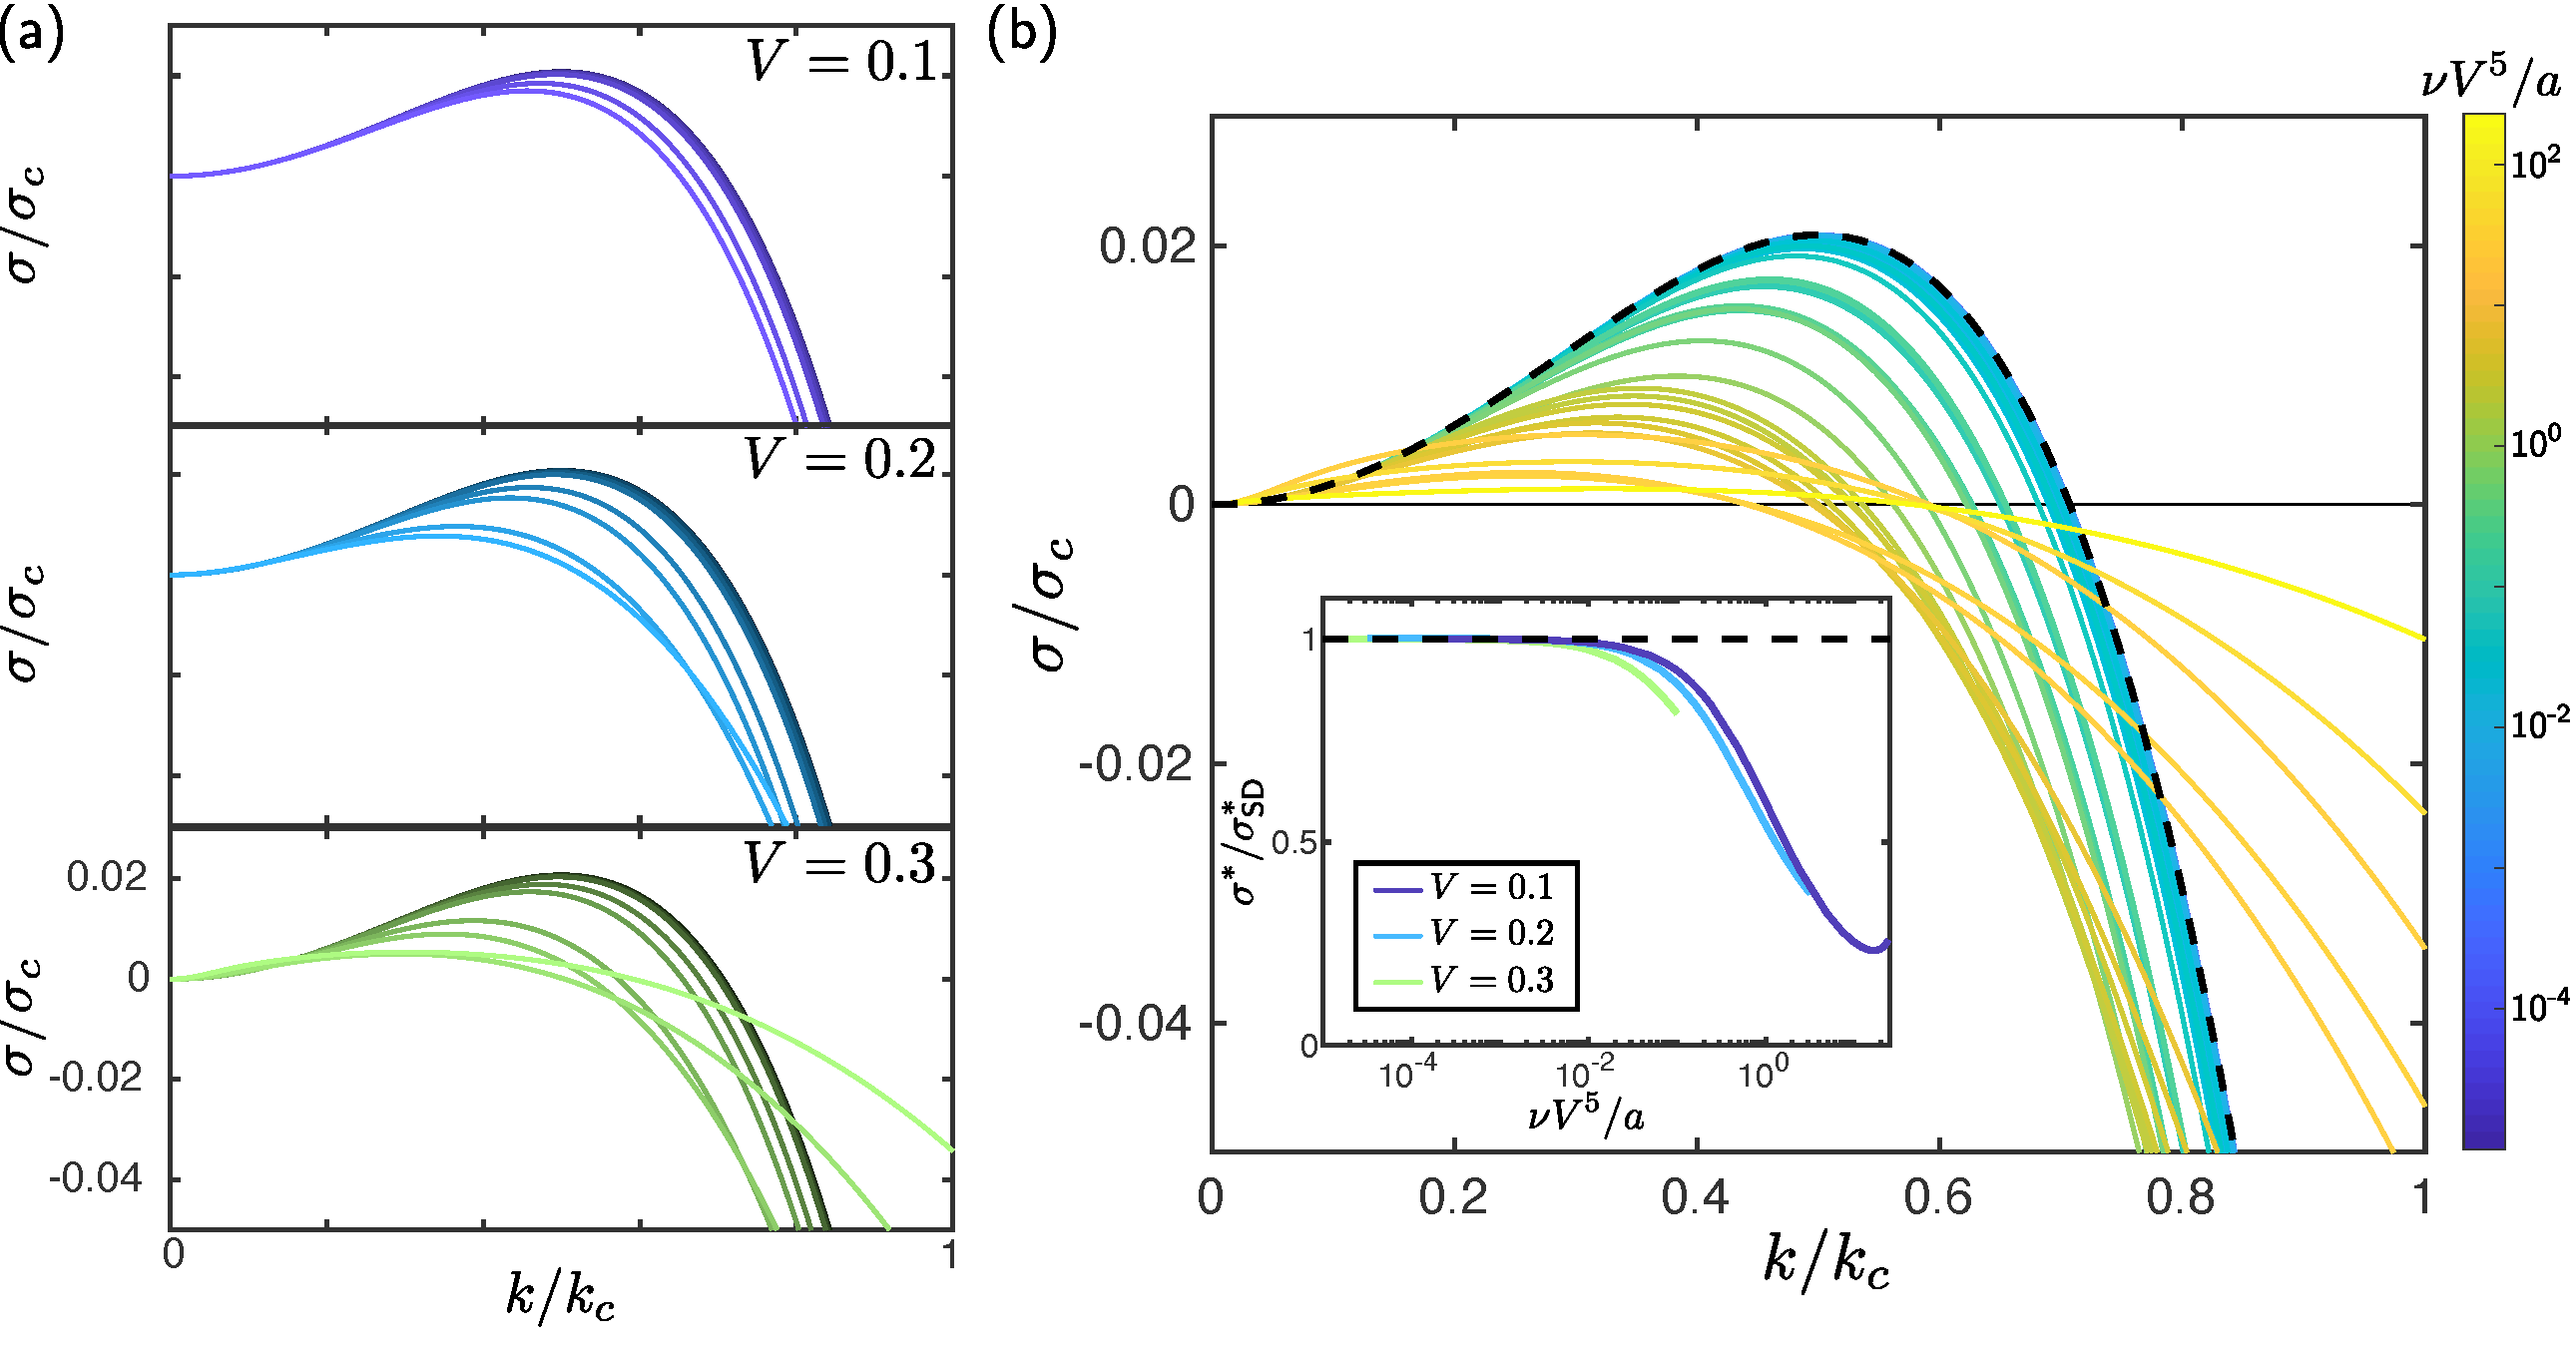
\includegraphics[width = \textwidth]{Collapsed_growth_rates}
\caption{(a) Numerically obtained dispersion relations $\sigma(k)$ rescaled according to~\eqref{E:InstabilityChapter:SlowCondensation:NumericalSols:DimensionlessScalings}. The value of the cross sectional volume $V$ used is indicated in each plot, and here $\aspect = 0.01$. Each curve corresponds to a different value of $\nu$, taking logarithmically spaced values between $10^{-2}$ and $10^{2}$; darker shaded curves corresponds to lower values of $\nu$. (b) Rescaled growth rates shown from (a) plotted on top of one another, and coloured according to $\nu V^5 /a$ (indicated by the colour bar); the results for $\nu V^5 /a \lesssim 10^{-2}$ are indistinguishable from the black dashed curve, which represents the asymptotic result~\eqref{E:InstabilityChapter:SlowCondensation:Asymptotics:SigmaResult}. Inset: semilogarithmic plot of the ratio between numerically obtained values of the maximum growth rate $\sigma^*$ and the asymptotic prediction $\sigma^*_{\textsf{SD}}$ given by~\eqref{E:InstabilityChapter:SlowCondensation:Asymptotics:FastestGrowingMode}.}
\label{fig:InstabilityChapter:SlowCondensation:CollapsedGrowthRates}
\end{figure}


\subsection{Asymptotics for small deformations}\label{S:InstabilityChapter:NoCondensation:SmallDeformations}
In this section, we provide details of an asymptotic analysis of the boundary value problem~\eqref{E:InstabilityChapter:SlowCondensation:Periodic:ODEwet}--\eqref{E:InstabilityChapter:SlowCondensation:Periodic:kinematic} in the case of small deformations. We aim to predict the envelope of growth rate curves in Figure~\ref{fig:InstabilityChapter:SlowCondensation:CollapsedGrowthRates} and thus predict the fastest growing mode and corresponding growth rate in this limit. Here we give an outline of the asymptotic analysis -- further details can be found in Appendix~\ref{A:InstabilityChapter:SmallDeformationAsymptotics}.

\subsubsection{Qualitative description of analysis}
As alluded to in \S\ref{S:InstabilityChapter:BaseState:Equilibria}, we encode small deformations by considering
\begin{equation}
\epsilon  = |\nu| V^4 \ll 1.
\end{equation}

The first step in the asymptotic analysis is to rescale the wavenumber by introducing $\K =k/k_c \sim \mathcal{O}(1)$ (when $k \sim k_c$ the two curvature contributions in the pressure boundary condition~\eqref{E:InstabilityChapter:SlowCondensation:Periodic:pressure_bc} balance). We anticipate the majority of the bending deformation occurs in the wet region $0 < x < x_0 = V + \mathcal{O}(\epsilon)$, and introduce the rescaled spatial variable $X = x/V$ to reflect this. In doing so,  the parameter $\param = \nu V^5 / a  = \epsilon  V/|a|$ naturally appears; $\xi$ describes the relative sizes of increases in-plane and transverse bending energies when the equilibrium is subject to a perturbation with wavenumber $k \sim k_c$. To see this we note that the typical (dimensionless) in-plane and transverse wall curvatures induced by this perturbation are
\begin{equation}
\kappa_{\text{in-plane}} \sim k_c^2 \Delta h \sim \frac{\nu V^3}{a} \Delta h \quad \text{and}\quad \kappa_{\text{transverse}} \sim \frac{\Delta h}{x_0^2} \sim  \frac{\Delta h}{V^2},
\end{equation}
where $\Delta h$ is the typical change in channel thickness that results from the perturbation. The corresponding dimensionless bending energies are
\begin{align}
E_{\text{in-plane}} &\sim \frac{\left(\kappa_{\text{in-plane}}\right)^2}{k_c} \sim \left( \frac{\nu V^3}{a}\right)^{3/2}(\Delta h)^2,\\ 
E_{\text{transverse}} &\sim x_0 \left(\kappa_{\text{transverse}}\right)^2 \sim \frac{(\Delta h)^2}{V^3},
\end{align}
whose ratio is
\begin{equation}
\frac{E_{\text{in-plane}}}{ E_{\text{transverse}}}
\sim \param^{3/2}.
\end{equation}

To make progress, we consider the limit $\param \to 0$. We pose a bivariate asymptotic expansion of the perturbation to the channel shape, $\Lambda$, the perturbation to the pressure, $\Pi$, and the growth rate, $\sigma$, in both $\epsilon$ and $\param$, using subscript $\left\{i,j\right\}$ to denote the term at $\mathcal{O}(\param^i \epsilon^j)$:
\begin{align}
\Lambda(X) &=    \Lambda_{0,0} + \param \Lambda_{1,0} + \epsilon \Lambda_{0,1} +  \param^2 \Lambda_{2,0} + \param \epsilon \Lambda_{1,1} + \epsilon^2 \Lambda_{0,2} + \dots,\label{E:InstabilityChapter:SlowCondensation:Asymptotics:ExpansionH} \\
\Pi(X) &=  \Pi_{0,0} + \param \Pi_{1,0} + \epsilon \Pi_{0,1} +  \param^2\Pi_{2,0} + \param \epsilon \Pi_{1,1} + \epsilon^2 \Pi_{0,2}+\dots,\label{E:InstabilityChapter:SlowCondensation:Asymptotics:ExpansionP} \\
\sigma(k) &= \sigma_{0,0} + \param \sigma_{1,0} + \epsilon \sigma_{0,1} +  \param^2 \sigma_{2,0} + \param \epsilon \sigma_{1,1} + \epsilon^2 \sigma_{0,2} + \dots. \label{E:InstabilityChapter:SlowCondensation:Asymptotics:ExpansionSigma}
\end{align}

\subsubsection{Results}
The particular hierarchy of problems arising from the asymptotic expansion~\eqref{E:InstabilityChapter:SlowCondensation:Asymptotics:ExpansionH}--\eqref{E:InstabilityChapter:SlowCondensation:Asymptotics:ExpansionSigma} depends on the relative sizes of $\epsilon$ and $\param$, but we must ensure that $V \gg |\aspect|$ for lubrication theory to remain valid, and therefore
$\param  = \epsilon (V/|a|) \gg \epsilon$ (in Appendix~\ref{A:InstabilityChapter:SmallDeformationAsymptotics}, we present the hierarchy of problems for the case $\epsilon \sim \param^2$). The leading order ($\mathcal{O}(1)$) and first order ($\mathcal{O}(\param)$) problems are, however, independent of the relationship between $\epsilon$ and $\param$.


In the leading order and first order problems, the pressure profile is a linear function of $X$. However, to satisfy the no flux condition at $X =0$, this pressure perturbation is, in fact, constant and thus offers no contribution to $\sigma$, i.e.
\begin{equation}
\sigma_{0,0} = 0 = \sigma_{1,0}.
\end{equation}
We find the leading order contribution to the perturbation to the channel shape to be
\begin{equation}
\Lambda_{0,0} =\nu V^3 \times \begin{cases}
\frac{X^2}{6}(X - 3) & 0 < X < 1,\\
\frac{1}{6}(1-X) & 1 < X < 1/V.
\end{cases}
\end{equation}
The leading order solution reflects a shear arising from the base state pressure (magnitude $\nu$) acting over a length equal to the amplitude of the perturbation, to deform the wall over a length comparable to $V$ (the shear force is the third derivative of the beam shape). Note that $\Lambda_{0,0}(X=1) < 0$ -- this allows us to verify that $\Lambda(x = x_0) < 0$ in the limit of small deformations, $|\nu| V^4 \to 0$ (as suggested in the previous section). We find the Poisson's ratio $\poisson$ in the first order term, $\Lambda_{1,0}$, but not in the leading order term, $\Lambda_{0,0}$, demonstrating that the contribution from the dry region enters at lower order (the Poisson's ratio only enters the problem via the boundary conditions on the dry region, at $x = 1$).

Despite the dependence of the hierarchy of problems on the relationship between $\epsilon$ and $\param$, the first non-zero term in the expansion of $\sigma$~\eqref{E:InstabilityChapter:SlowCondensation:Asymptotics:ExpansionSigma} is
\begin{equation}\label{E:InstabilityChapter:SlowCondensation:Asymptotics:LeadingOrderSigma}
\sigma_{1,1} = \frac{K^2\left(1-2K^2\right)}{6V^2},
\end{equation}
regardless of the relationship between $\epsilon$ and $\param$. (The first non-zero term in the expansion~\eqref{E:InstabilityChapter:SlowCondensation:Asymptotics:ExpansionP} is the $\mathcal{O}(\epsilon)$ term, $\Pi_{0,1}$, because the terms corresponding to the destabilizing transverse curvature, and stabilizing in-plane curvature contributions to the pressure enter at this order.  However, we find that $\Pi_{0,1}$ is constant, and the first term in~\eqref{E:InstabilityChapter:SlowCondensation:Asymptotics:ExpansionP} with a non-zero gradient -- which sets the growth rate -- comes in at the next order, $\mathcal{O}(\epsilon \param)$.)

Noting that $\sigma_c = \epsilon\param/V^2$ and substituting~\eqref{E:InstabilityChapter:SlowCondensation:Asymptotics:LeadingOrderSigma} in to the expansion~\eqref{E:InstabilityChapter:SlowCondensation:Asymptotics:ExpansionSigma}, gives
\begin{equation}\label{E:InstabilityChapter:SlowCondensation:Asymptotics:SigmaResult}
\frac{\sigma(K)}{\sigma_c} =  \frac{K^2\left(1-2K^2 \right)}{6}  + \mathcal{O}(\param).
\end{equation}
Equation~\eqref{E:InstabilityChapter:SlowCondensation:Asymptotics:SigmaResult} gives the envelope of the curves $\sigma(k)$ (Figure~\ref{fig:InstabilityChapter:SlowCondensation:CollapsedGrowthRates}(b)). Moreover, and as expected, numerical solutions with larger values of $\param = \nu V^5 /|a|$ deviate more significantly from this envelope.

By maximizing~\eqref{E:InstabilityChapter:SlowCondensation:Asymptotics:SigmaResult} with respect to $K$, we find that the small deformation estimates of the fastest growing mode, denoted $k^*_{\textsf{SD}}$, and the corresponding growth rate, denoted $\sigma^*_{\textsf{SD}}$ are
\begin{equation}\label{E:InstabilityChapter:SlowCondensation:Asymptotics:FastestGrowingMode}
\sigma^*_{\textsf{SD}}= \frac{1}{48}\sigma_c = \frac{1}{48}\frac{\nu^2 V^7}{\aspect}, \qquad k^*_{\textsf{SD}}= \frac{1}{2}k_c = \frac{1}{2}\sqrt{\frac{\nu V^3}{\aspect}}.
\end{equation}
which agree well with numerical solutions of the BVP (see inset of Figure~\ref{fig:InstabilityChapter:SlowCondensation:CollapsedGrowthRates}(b), in which perfect agreement would correspond to $y = 1$). Numerical solutions with larger values of $V$ -- and thus larger values of $\epsilon = |\nu| V^4$ for a given $\nu$ -- peel off from the asymptotic prediction~\eqref{E:InstabilityChapter:SlowCondensation:Asymptotics:FastestGrowingMode} at a lower value of $\delta$, as we would expect.

The numerically obtained values of $\sigma^*/\sigma^*_{\textsf{SD}}$ are not monotonic in $\param = \nu V^5/a$ (see the $V = 0.1$ curve in the inset of Figure~\ref{fig:InstabilityChapter:SlowCondensation:CollapsedGrowthRates}(b)). As $\param$ increases, the penalizing effect of in-plane bending tends to suppress the growth rate relative to the asymptotic result ($\sigma^*/\sigma^*_{\textsf{SD}}$ initially decreases). For a given value of $\aspect$, increases in $\param = \nu V^5/|a|$ are, however, accompanied by increases in the deformation parameter $\epsilon = |\nu| V^4$ allowing the non-linear effects of significant base state deformation to enter. Specifically, the competition between the non-linearities in channel permeability and meniscus pressure (which tend to reduce and enhance the growth rate of instability, respectively) is won by the former, and the net effect of the channel width non-linearity is to enhance the growth rate relative to $\sigma^*_{\text{SD}}$. (This is reminiscent of the `over-shooting' of the asymptotic result by numerical solutions observed in Chapter 2.)

Note that our prediction of the fastest growing mode and the corresponding growth rate are highly sensitive to the amount of liquid in the channel via the volume $V$ ($\sigma \sim V^7$ for small deformations~\eqref{E:InstabilityChapter:SlowCondensation:Asymptotics:FastestGrowingMode}); we might expect, therefore, that if the volume is changing, then the fastest growing mode will be changing as well. We turn now to consider the case of non-zero condensation to describe formally how the mode selection problem changes when the liquid is being added via condensation.

\section{The influence of condensation}
In this section, we consider the case when $C>0$, and liquid is added to the channel via condensation. We focus on how mode selection in the competing curvature instability described in the previous section, is modified by the presence of a dynamic base state and a non-constant liquid volume that result from a non-zero condensation rate.

\subsection{Base State}
With $C>0$, equilibria of the model equations~\eqref{E:InstabilityChapter:Modelling:NonDim:ClampedBC}--\eqref{E:InstabilityChapter:Modelling:NonDim:Kinematic} do not exist. In this case, the base state configurations are those with a cylindrical interface:
\begin{equation}\label{E:InstabilityChapter:BaseState:FlatInterface:FlatAnsatz}
h = h_0(x,t), \qquad p = p_0(x,t), \qquad \x_m  = \x_0(\that).
\end{equation}

Substituting~\eqref{E:InstabilityChapter:BaseState:FlatInterface:FlatAnsatz} into the model equations~\eqref{E:InstabilityChapter:Modelling:NonDim:ClampedBC}--\eqref{E:InstabilityChapter:Modelling:NonDim:Kinematic}  results in a system of spatially one dimensional PDEs:
\begin{align}
\ddp{h_0}{t} & = \frac{1}{3|\nu|}\ddp{}{x}\left(h_0^3 \ddp{p_0}{x}\right) & &0 < x < x_0,\label{E:InstabilityChapter:BaseState:FlatInterface:PDEwet}\\
 p_0 &=0 & & x_0 < x < 1,\label{E:InstabilityChapter:BaseState:FlatInterface:PDEdry}\\
p_0 &= \ddp{^4 h_0}{x^4} & & 0 < x < 1.\label{E:InstabilityChapter:BaseState:FlatInterface:pressure2shape}
\end{align}
with boundary conditions
\begin{align}
h_0 &= 1, ~\ddp{h_0}{x} = 0, ~\ddp{p_0}{x} = 0 & &\text{at}~x = 0,\label{E:InstabilityChapter:BaseState:FlatInterface:bc0}\\
p_0 &= -\frac{\nu}{h_0}& &\text{at}~x = x_0,\label{E:InstabilityChapter:BaseState:FlatInterface:pressurebc}\\
\ddp{^2 h_0}{x^2} &=0,~ \ddp{^3 h_0}{x^3} = 0 & &\text{at}~x = 1,\label{E:InstabilityChapter:BaseState:FlatInterface:bc1}
\end{align}
\begin{equation}\label{E:InstabilityChapter:BaseState:FlatInterface:jumpbc}
\left[h_0\right]_{x_0^-}^{x_0^+} = \left[\ddp{h_0}{x}\right]_{x_0^-}^{x_0^+}   = \left[\ddp{^2 h_0}{x^2}\right]_{x_0^-}^{x_0^+} = \left[\ddp{^3 h_0}{x^3 }\right]_{x_0^-}^{x_0^+}   = 0,
\end{equation}
and a kinematic condition
\begin{equation}\label{E:InstabilityChapter:BaseState:FlatInterface:kinematicbc}
\ddp{x_0}{t} = -\frac{h_0^2}{3|\nu|}\left.\ddp{p_0}{x}\right|_{x = x_0} + C.
\end{equation}

The associated cross-sectional volume is now time-dependent,
\begin{equation}\label{E:InstabilityChapter:BaseState:FlatInterface:cross_sect_volume}
V(t) = \int_0^{x_0(t)} \h_0(x, t) ~\mathrm{d}x,
\end{equation}
and its initial value is denoted by $V_0 = V(t = 0)$.
We take the pressure and channel shape from the $C = 0$ equilibrium that has volume $V = V_0$ (as described in \S\ref{S:InstabilityChapter:BaseState:Equilibria}) to be the initial condition on~\eqref{E:InstabilityChapter:BaseState:FlatInterface:PDEwet}--\eqref{E:InstabilityChapter:BaseState:FlatInterface:kinematicbc} (this implicitly specifies the initial condition $x_0(t=0)$).

\subsubsection{Base state dynamics}\label{S:InstabilityChapter:WithCondensation:BaseStateDynamics}
Before moving on to analyze the stability of these base states to in-plane perturbations, we consider how the condensation rate affects their dynamic behaviour by solving equations~\eqref{E:InstabilityChapter:BaseState:FlatInterface:PDEwet}--\eqref{E:InstabilityChapter:BaseState:FlatInterface:kinematicbc} numerically. The numerical scheme used to solve these equations is very similar to that described in \S2.2 for the equations describing bendotaxis in a single flexible channel, but with a single meniscus and a no-flux boundary condition applied at $x = 0$.  Full details of this numerical scheme can be found in Appendix~\ref{A:Chapter6:Numerics}.

\begin{figure}[t]
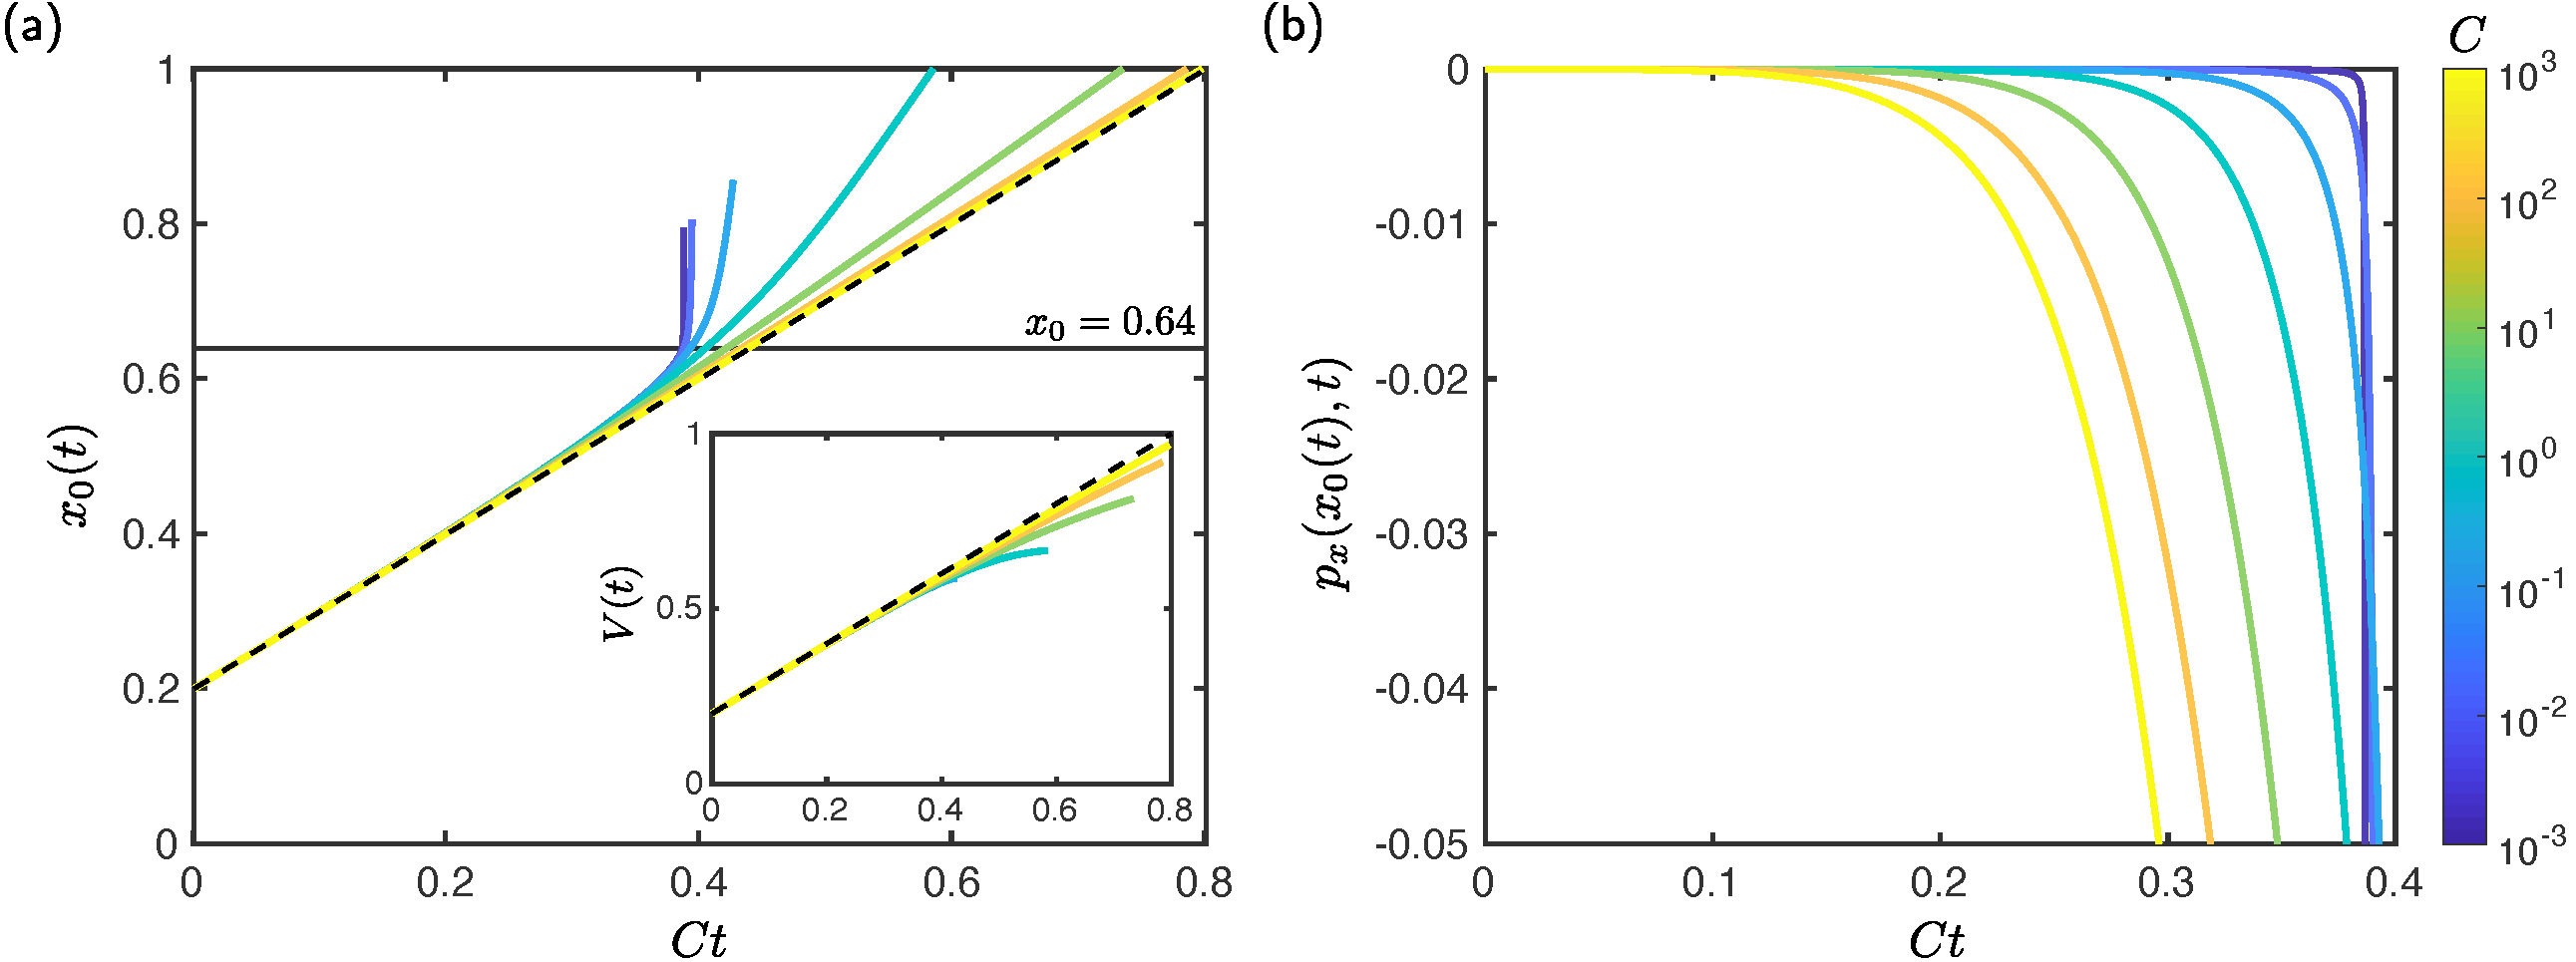
\includegraphics[width = \textwidth]{base_state_dynamicsv2}
\caption{ (a) Meniscus position, $x_0(t)$, and (b) pressure gradient at the meniscus, $p_x(x_0(t),t)$ (using subscript to denote a partial derivative with respect to $x$), in numerical solutions of base state equations~\eqref{E:InstabilityChapter:BaseState:FlatInterface:PDEwet}--\eqref{E:InstabilityChapter:BaseState:FlatInterface:kinematicbc} with $\nu = 10$, $V_0 = 0.2$. The colour of the curves indicates the condensation rate $C$ as specified in the colour bar in (b). The dashed lines in (a) indicates a linear increase in meniscus position, $x_0 = x_0(t = 0) + Ct$; the trajectories in (a) diverge from this linear prediction when $x_0 \approx 0.64$, the moment at which the corresponding $C = 0$ equilibrium goes unstable (see Figure~\ref{fig:InstabilityChapter:FlatInterface:NoCond:Tv12_analogue}). Inset: the cross sectional volume $V(t)$ in the numerical solutions of (a). The dashed line indicates $V = V_0 + Ct$. }\label{E:InstabilityChapter:WithCondensation:BaseState:Dynamics}
\end{figure}

Meniscus trajectories, $x_0(t)$, alongside the pressure gradient at the meniscus, $p_x(x_0)$, are shown in Figure~\ref{E:InstabilityChapter:WithCondensation:BaseState:Dynamics} for different values of the condensation rate $C$. The pressure gradient at the meniscus acts as a proxy for the dynamic behaviour in the base state -- deviations away from zero indicate non quasi-static behaviour of the base state.


When condensation in slow, $C \ll 1$, the behaviour can be  split into two distinct time periods. At early times  (see $t \lesssim 0.4$ in Figure~\ref{E:InstabilityChapter:WithCondensation:BaseState:Dynamics}), meniscus position follows $x_0 = V_0 + Ct$ and the base state evolves quasi-statically; condensation simply marches the system through the true equilibria with $C = 0$, whose volume is the instantaneous volume $V(t)$. However, at the  time (and thus volume) at which the corresponding $C =0$ equilibrium becomes unstable to uniform perturbations (in this example, this occurs when $x_0 \approx 0.64$, see Figure~\ref{fig:InstabilityChapter:FlatInterface:NoCond:Tv12_analogue}) the behaviour ceases to be quasistatic because the evolution of this instability is much faster than the condensation driven evolution. Beyond this point, the dynamics are driven by the instability -- the meniscus advances faster than the speed set by condensation, and ultimately the numerical integration terminates with channel walls touching before the meniscus reaches the free end of the channel. In this section, however, we shall consider only sufficiently early times (sufficiently low $V(t)$) that the corresponding $C =0$ equilibria are linearly stable to uniform perturbations. Therefore $C\ll 1$ will be considered to correspond to quasi-static behaviour in which condensation only influences the cross sectional volume $V(t)$.

When condensation is fast, $C \gtrsim 1$, the meniscus position follows the motion $x_0 = V_0 + Ct$ set by condensation throughout. In particular, the meniscus position does not deviate from this when the corresponding $C = 0$ equilibrium goes unstable (i.e.~at $t \approx 0.4$) because the time scale of evolution of this instability is much longer than the time scale $1/C$ set by condensation in this case. We see from Figure~\ref{fig:InstabilityChapter:FlatInterface:NoCond:Tv12_analogue}(b) that the base state dynamics are `excited' before the corresponding $C = 0$ equilibria goes unstable (before  $t \approx 0.4$), indicating that condensation driven dynamics in the base state are important in this case; for $C \gtrsim 1$, condensation exerts control over both the volume $V(t)$ and induces dynamic behaviour in the base state.

Before moving on to consider the stability of this base state to in-plane perturbations, we note that the liquid volume only deviates from $V = V_0 + Ct$ at late times (see inset in Figure~\ref{fig:InstabilityChapter:FlatInterface:NoCond:Tv12_analogue}(a)) when the menisci are near to the free end, and channel deformations are significant.

\subsection{Frozen time approximation}\label{S:InstabilityChapter:WithCondensation:FrozenTime}
In the previous section, we saw that when $C \ll 1$, condensation exerts little control on the base state dynamics, and its influence is to increase the cross sectional volume $V(t)$ only. If we assume that condensation exerts no control at all on the base state dynamics, then the condensation rate simply marches the system through the true equilibria with $C = 0$ described in \S\ref{S:InstabilityChapter:BaseState:Equilibria}. With this assumption, the instantaneous growth rate of a mode with wavenumber $k$ and amplitude $x_1$ will be the $C = 0$ result at the current value of $V$, i.e.
\begin{equation}\label{E:InstabilityChapter:NonZeroCond:Quasistatic:InstantaneousSigma}
\frac{1}{x_1}\dd{x_1}{t} = \sigma_{C=0}\left[V(t);\nu, \aspect,k\right],
\end{equation}
where $\sigma_{C=0}$ is the growth rate obtained with $C = 0$.

The asymptotic analysis for small deformations described in \S\ref{S:InstabilityChapter:NoCondensation:SmallDeformations} showed that
\begin{equation}\label{E:InstabilityChapter:NonZeroCond:Quasistatic:InstantaneousSigmaAsymptotic}
 \sigma_{C=0}\left[V(t);\nu, \aspect,k\right] \approx \frac{\nu^2 V(t)^7}{|\aspect|}f\left(\frac{k}{k_c}\right)\quad \text{for}~|\nu| V^4 \ll 1,
\end{equation}
where
\begin{equation}\label{E:InstabilityChapter:NonZeroCond:Quasistatic:InstantaneousSigmaAsymptoticSpecifics}
f(\zeta) = \frac{\zeta^2}{6}\left(1-2\zeta^2 \right), \qquad k_c = k_c(t) = \sqrt{\frac{\nu V(t)^3}{\aspect}}.
\end{equation}
In addition, the volume increases linearly with time when deformations are small,
\begin{equation}
V(t) = V_0 + Ct.
\end{equation}

The sensitive dependence of the growth rate $ \sigma_{C=0}$ on $V$ means that the modes that are initially growing (those with $k/k_c(t= 0) = k/\sqrt{\nu V_0^3 / a} < 1/\sqrt{2}$), do so very slowly. As time progresses, and the volume increases, the band of unstable modes grows, as does the growth rate of these newly unstable modes. The growth rate of the modes that were initially unstable increases, but more slowly. Eventually, the higher, later `starting', modes will be growing faster than the initially growing modes and may therefore catch-up with, and overtake, the initially growing modes (which have lower wavenumber). Ultimately, we expect that the pattern observed at late times will correspond to the mode that is first to reach the non-linear regime, and so this increase of wavenumber (instability refinement) will not continue indefinitely.

\begin{figure}[t]
\centering
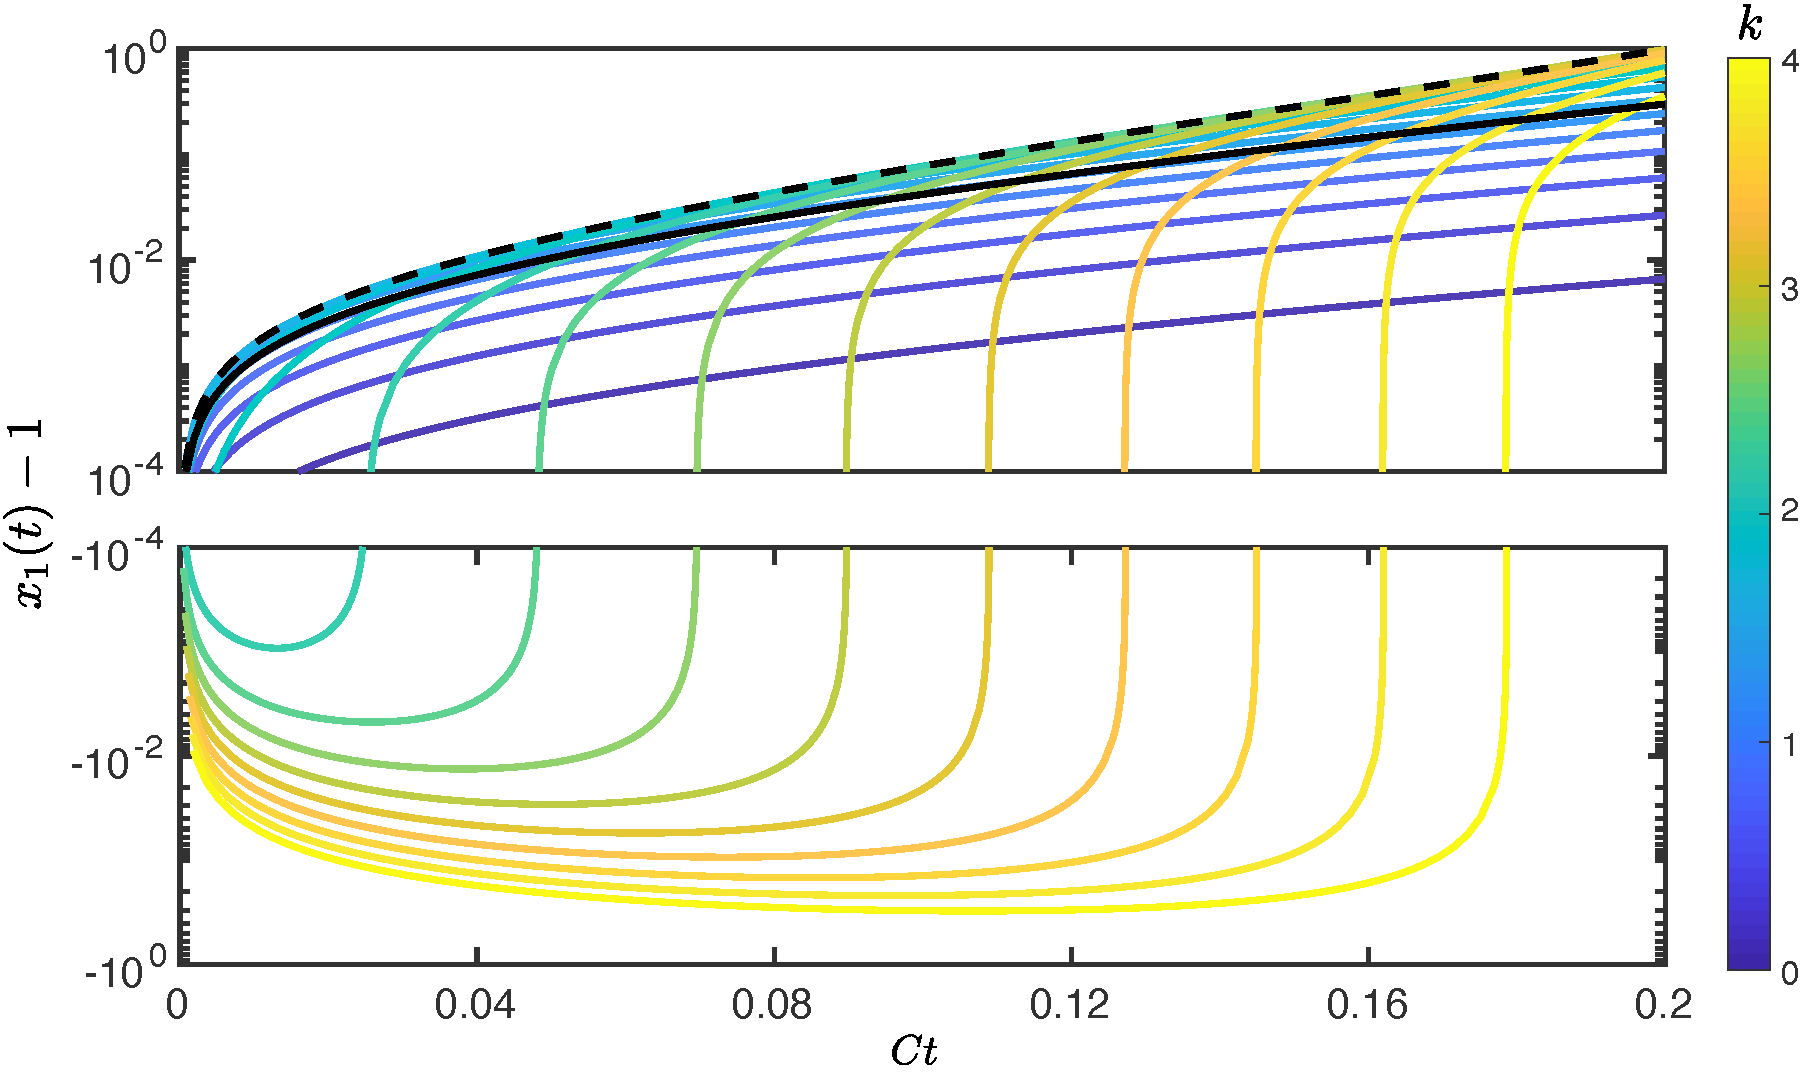
\includegraphics[width = 0.8\textwidth]{overtake_with_asymptotics_and_bvp}
\caption{Growth of the amplitude of the mode of wavenumber $k$ as a function of time as calculated from the ODE~\eqref{E:InstabilityChapter:NonZeroCond:Quasistatic:AsymptoticODE}  with $V_0 = 0.2$, and $\nu = 10$, $a = 0.01$. The upper and lower plots corresponds to increase and decrease of the amplitude of modes, respectively. The colour of the curves indicates the wavenumber $k$, as specified by the colour bar. Also plotted are the envelope of these solutions for small deformations (equation~\eqref{E:InstabilityChapter:NonZeroCond:Quasistatic:AsymptoticODE_envelopeSigma}, black dashed line) and the corresponding envelope for the ODE~\eqref{E:InstabilityChapter:NonZeroCond:Quasistatic:InstantaneousSigma} (solid black curve).}
\label{fig:InstabilityChapter:NonZeroCond:QuasistaticOvertake}
\end{figure}

To demonstrate this possibility explicitly, we consider the small deformation approximation of~\eqref{E:InstabilityChapter:NonZeroCond:Quasistatic:InstantaneousSigma}. Using a tilde to denote this approximation, we have
\begin{equation}\label{E:InstabilityChapter:NonZeroCond:Quasistatic:AsymptoticODE}
\frac{1}{\tilde{x}_1}\dd{\tilde{x}_1}{t}  = \frac{\nu^2 V(t)^7}{\aspect}f\left(\frac{k}{k_c(t)}\right).
\end{equation}
The solution to~\eqref{E:InstabilityChapter:NonZeroCond:Quasistatic:AsymptoticODE} with initial condition $\tilde{x}_1(t = 0) = 1$ is
\begin{equation}\label{E:InstabilityChapter:NonZeroCond:Quasistatic:AsymptoticODE_sol}
\tilde{x}_1= \exp\left\{-\frac{k^2}{6C}\left[|\aspect| k^2 \left(V(t)^2 - V_0^2\right) - \frac{|\nu|}{5}\left(V(t)^5 - V_0^5\right)\right]\right\}.
\end{equation}

We plot in Figure~\ref{fig:InstabilityChapter:NonZeroCond:QuasistaticOvertake} the growth of the amplitude $\tilde{x}_1$ given by~\eqref{E:InstabilityChapter:NonZeroCond:Quasistatic:AsymptoticODE_sol} for various $k$ in which this overtaking mechanism can be seen. At early times, the largest modes are those with small wavenumber (dark curves in Figure~\ref{fig:InstabilityChapter:NonZeroCond:QuasistaticOvertake}), and modes with larger wavenumbers (lighter curves in~\ref{fig:InstabilityChapter:NonZeroCond:QuasistaticOvertake}) decay. However, at later times these modes with larger wavenumber enter into the unstable band and so begin to grow. Some of these modes overtake the smaller wavenumber modes, but those solutions with the largest wavenumbers (the lightest curves in Figure~\ref{fig:InstabilityChapter:NonZeroCond:QuasistaticOvertake}) do not spend enough time in the unstable band to be able to overtake the smaller wavenumber modes before the solution ends with $V(t) = 0.4$.

By maximizing the solution~\eqref{E:InstabilityChapter:NonZeroCond:Quasistatic:AsymptoticODE_sol} with respect to wavenumber $k$, we find that the instantaneously largest mode is
\begin{equation}\label{E:InstabilityChapter:NonZeroCond:Quasistatic:AsymptoticODE_envelopeK}
\tilde{k}_{\textsf{max}}(t) = \sqrt{\frac{\nu}{10\aspect}\frac{V(t)^5 - V_0^5}{V(t)^2 - V_0^2}}.
\end{equation}
The maximum displacement
\begin{equation}\label{E:InstabilityChapter:NonZeroCond:Quasistatic:AsymptoticODE_envelopeSigma}  \tilde{A}_{\text{max} }= \tilde{x}_1\left(t; \tilde{k}_{\text{max}}(t)\right) = \exp \left[\frac{\nu^2}{600C}\frac{\left(V(t)^5 - V_0^5\right)^2}{V(t)^2 - V_0^2}\right]
\end{equation}
describes the envelope of the curves in Figure~\ref{fig:InstabilityChapter:NonZeroCond:QuasistaticOvertake}.

We can find the corresponding envelope valid for (quasistatic) deformations of any size (i.e. not reasonably small) by numerically integrating~\eqref{E:InstabilityChapter:NonZeroCond:Quasistatic:InstantaneousSigma} to find $x_1$ for a range of values of $k$. We use the \texttt{ODE15s} routine implemented in \textsc{matlab} to perform this integration; the growth rate $\sigma_{C=0}$ is evaluated at each time step by solving the quasistatic BVP~\eqref{E:InstabilityChapter:SlowCondensation:Periodic:ODEwet}--\eqref{E:InstabilityChapter:SlowCondensation:Periodic:kinematic} numerically (as described in \S\ref{S:InstabilityChapter:NoCond:Numerics}). The envelope for deformation of any size is tighter than the envelope for small deformations as expected (Figure~\ref{fig:InstabilityChapter:NonZeroCond:QuasistaticOvertake}); numerically obtained values of $\sigma_{C=0}$ are smaller than the corresponding asymptotic approximations, which do not account for the in-plane bending penalty, as discussed in \S\ref{S:InstabilityChapter:NoCondensation:SmallDeformations}.

The analysis of this section serves to demonstrate the overtaking mechanism, and is expected to be valid for $C \ll 1$. To go beyond these results and describe the effect of non-zero condensation rate on mode selection for a general $C$, we must consider the equations describing perturbations from a time-dependent base state, to which we turn now.


\subsection{Periodic perturbations}
To analyze the linear stability of a time-dependent base state to periodic in-plane perturbations, we substitute the ansatz
\begin{align}
h &= h_0(x,t) + \epsilon h_1(x,t)\exp(iky), \\
 p &= p_0(x,t) +\epsilon p_1(x,t) \exp(iky), \\
  x_m &= x_0(t) +\epsilon x_1(t)\exp(iky),
\end{align}
where $\epsilon \ll 1$ is arbitrary, into the model equations~\eqref{E:InstabilityChapter:Modelling:NonDim:PDE1}--\eqref{E:InstabilityChapter:Modelling:NonDim:Kinematic}. Here $h_0, p_0, x_0$ satisfy the base-state equations~\eqref{E:InstabilityChapter:BaseState:FlatInterface:PDEwet}--\eqref{E:InstabilityChapter:BaseState:FlatInterface:kinematicbc}. Linearizing in $\epsilon$ results in a system of spatially one dimensional PDEs:
\begin{align}
\ddp{h_1}{t} &= \frac{1}{3|\nu|} \left[\ddp{}{x}\left(h_0^3 \ddp{p_1}{x} + 3h_0^2 \ddp{p_0}{x}H_1\right)- k^2 h_0^3 p_1\right] & &0 < x < x_0(t), \label{E:InstabilityChapter:WithCondensation:LinearizedEquations:PDEs1}\\
p_1&=0 & & x_0(t) < x < 1.\label{E:InstabilityChapter:WithCondensation:LinearizedEquations:PDEs2}\\
p_1 &= \ddp{^4 h_1}{x^4} - 2k^2 \ddp{^2 h_1}{x^2} + k^4 h_1 & & 0 < x < 1.\label{E:InstabilityChapter:WithCondensation:LinearizedEquations:Pressure2Shape}
\end{align}
The PDEs~\eqref{E:InstabilityChapter:WithCondensation:LinearizedEquations:PDEs1}--\eqref{E:InstabilityChapter:WithCondensation:LinearizedEquations:Pressure2Shape} are subject to the boundary and continuity conditions
\begin{align}
h_1 &= 0 = \ddp{h_1}{x} = \ddp{p_1}{x} = 0 & &\text{at}~x = 0,\label{E:InstabilityChapter:WithCondensation:LinearizedEquations:bc_x=0}\\
p_1 + x_1 \ddp{p_0}{x} &=\frac{\nu}{\h_0^2}\left(x_1\dd{h_0}{x} + h_1\right) + \nu \aspect  k^2 x_1, & &\text{at}~x = x_0.\label{E:InstabilityChapter:WithCondensation:LinearizedEquations:PressureBC}\\
\ddp{^2 h_1}{x^2} - \eta k^2 h_1 &= 0 = \ddp{^3 h_1}{x^2} - (2-\eta) k^2 h_1 & & \text{at}~x = 1.\label{E:InstabilityChapter:WithCondensation:LinearizedEquations:bc_x=1}
\end{align}
\begin{equation}\label{E:InstabilityChapter:WithCondensation:LinearizedEquations:JumpConditions}
\left[h_1\right]_{x_0^-}^{x_0^+} =  \left[\dd{h_1}{\x}\right]_{x_0^-}^{x_0^+} =   \left[\dd{^2h_1}{\x^2}\right]_{x_0^-}^{x_0^+} =  0, \qquad   \left[\dd{^3h_1}{\x^3}\right]_{x_0^-}^{x_0^+}  = \frac{\nu x_1}{h_0(x_0,t)}.
\end{equation}
The perturbation to the meniscus position evolves according to
\begin{equation}\label{E:InstabilityChapter:WithCondensation:LinearizedEquations:kinematic}
\dd{x_1}{t} =-\frac{1}{3|\nu|}\left.\left[ h_0^2 \ddp{p_1}{x} + x_1 \ddp{}{x}\left(h_0^2 \ddp{p_0}{x} \right) + 2 h_0 \ddp{p_0}{x} h_1 \right]\right|_{x = x_0}.
\end{equation}


\subsection{Numerical solutions}
In this section, we describe numerical solutions of the system of linear PDEs~\eqref{E:InstabilityChapter:WithCondensation:LinearizedEquations:PDEs1}--\eqref{E:InstabilityChapter:WithCondensation:LinearizedEquations:kinematic}. These equations are solved simultaneously alongside equations~\eqref{E:InstabilityChapter:BaseState:FlatInterface:PDEwet}--\eqref{E:InstabilityChapter:BaseState:FlatInterface:kinematicbc} describing the base state shape $h_0$, pressure $p_0$ and meniscus position $x_0$. Full details of the numerical scheme are contained in Appendix~\ref{A:Chapter6:Numerics}, but we point in particular to our choice of initial conditions; we anticipate that, as in the zero-condensation case, there are two branches of solutions, one of which has very high decay rates for all $k$ and one of which displays positive growth rates for sufficiently small $k$. To guide our numerics onto the branch displaying positive growth rates, we take the solution to the zero-condensation BVP~\eqref{E:InstabilityChapter:SlowCondensation:Periodic:ODEwet}--\eqref{E:InstabilityChapter:SlowCondensation:Periodic:kinematic} with $V = V_0$ that is on the `correct' branch to be the initial condition on $h_1$ and $p_1$ (with $x_1(0) = 1$ without loss of generality).

\subsubsection{Results}

\begin{figure}[t]
\centering
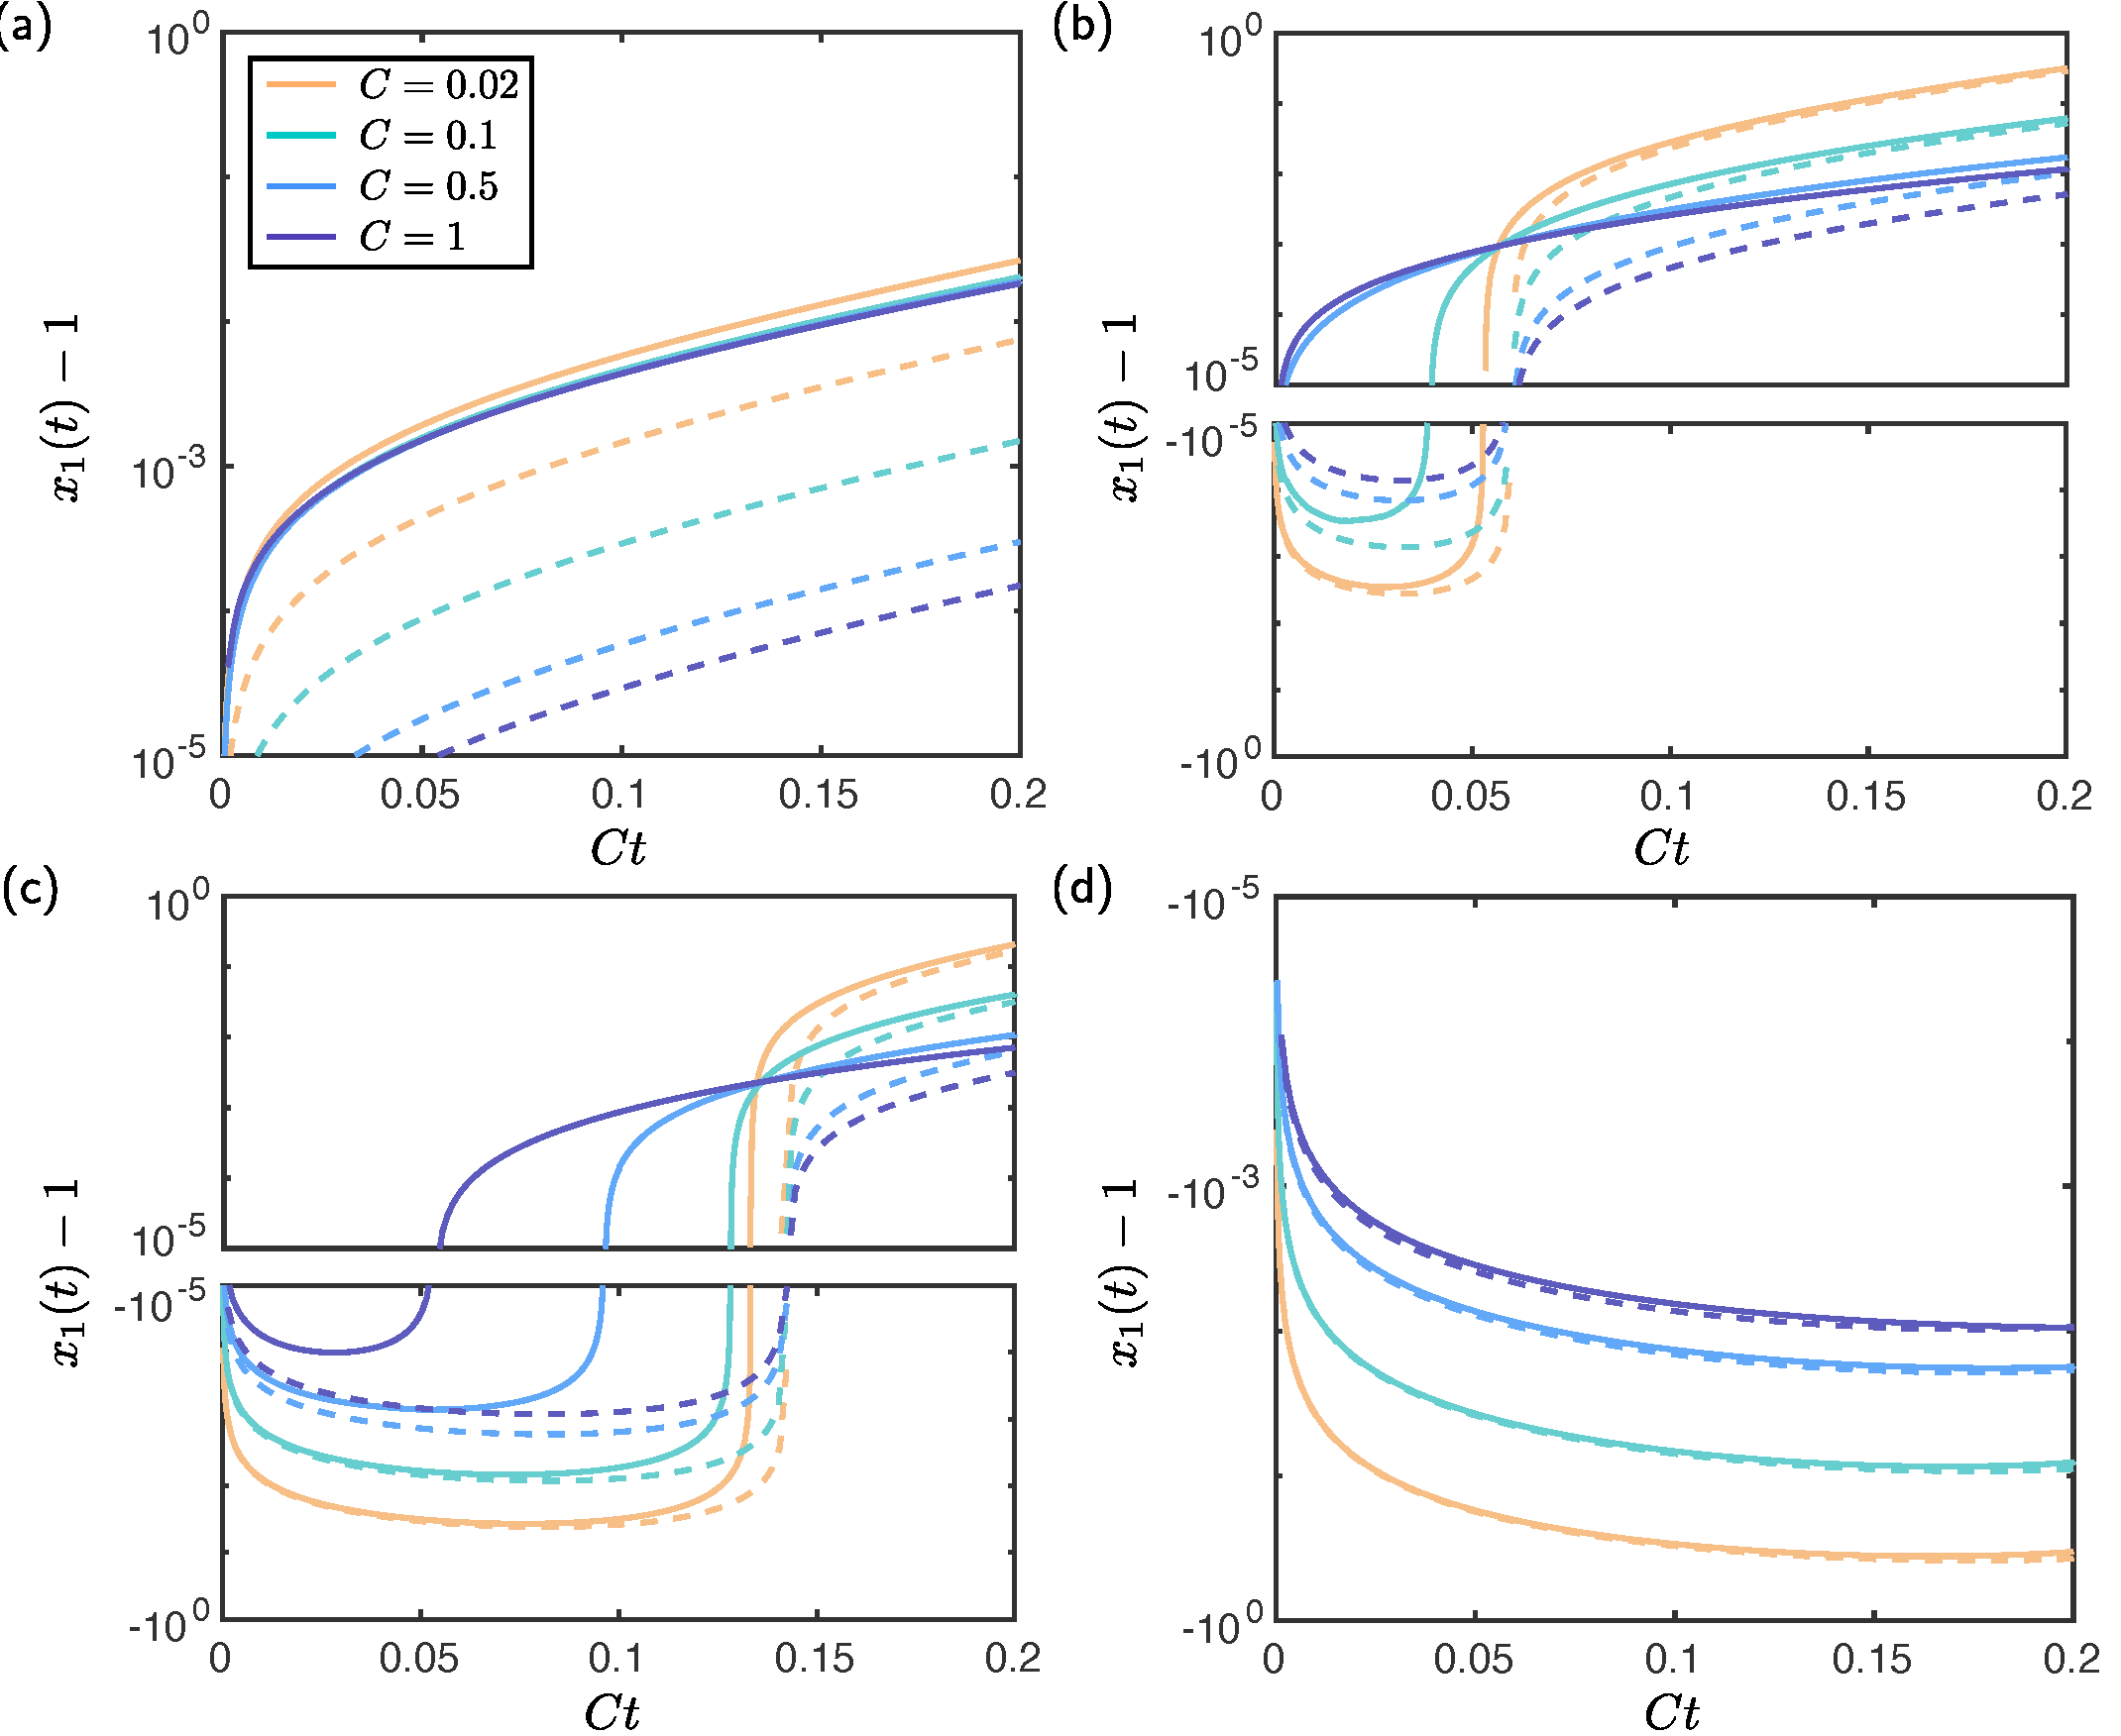
\includegraphics[width = 0.9\textwidth]{v2_full_numerics_traces}
\caption{Numerically obtained displacements, $x_1(t) -1$, of a perturbation to the meniscus position with wavenumber $k$. Data are shown for various condensation rates $C$ (see legend in (a)) and $\nu = 10$, $\aspect = 0.01$, $V_0 = 0.2$. The three plots correspond to  different wavenumbers as follows: (a) $k = 0.2$, (b) $k = 2.1$, (c) $k = 2.6$, and (c) $k = 3.9$. Each trajectory is accompanied by a dashed curve indicating the corresponding quasistatic behaviour, obtained by solving~\eqref{E:InstabilityChapter:NonZeroCond:Quasistatic:InstantaneousSigma} numerically with a linear volume increase, $V(t) = V_0 + Ct$.}
\label{fig:InstabilityChapter:TimeDepBaseState:FullNumericsTraces}
\end{figure}

\begin{figure}[t!]
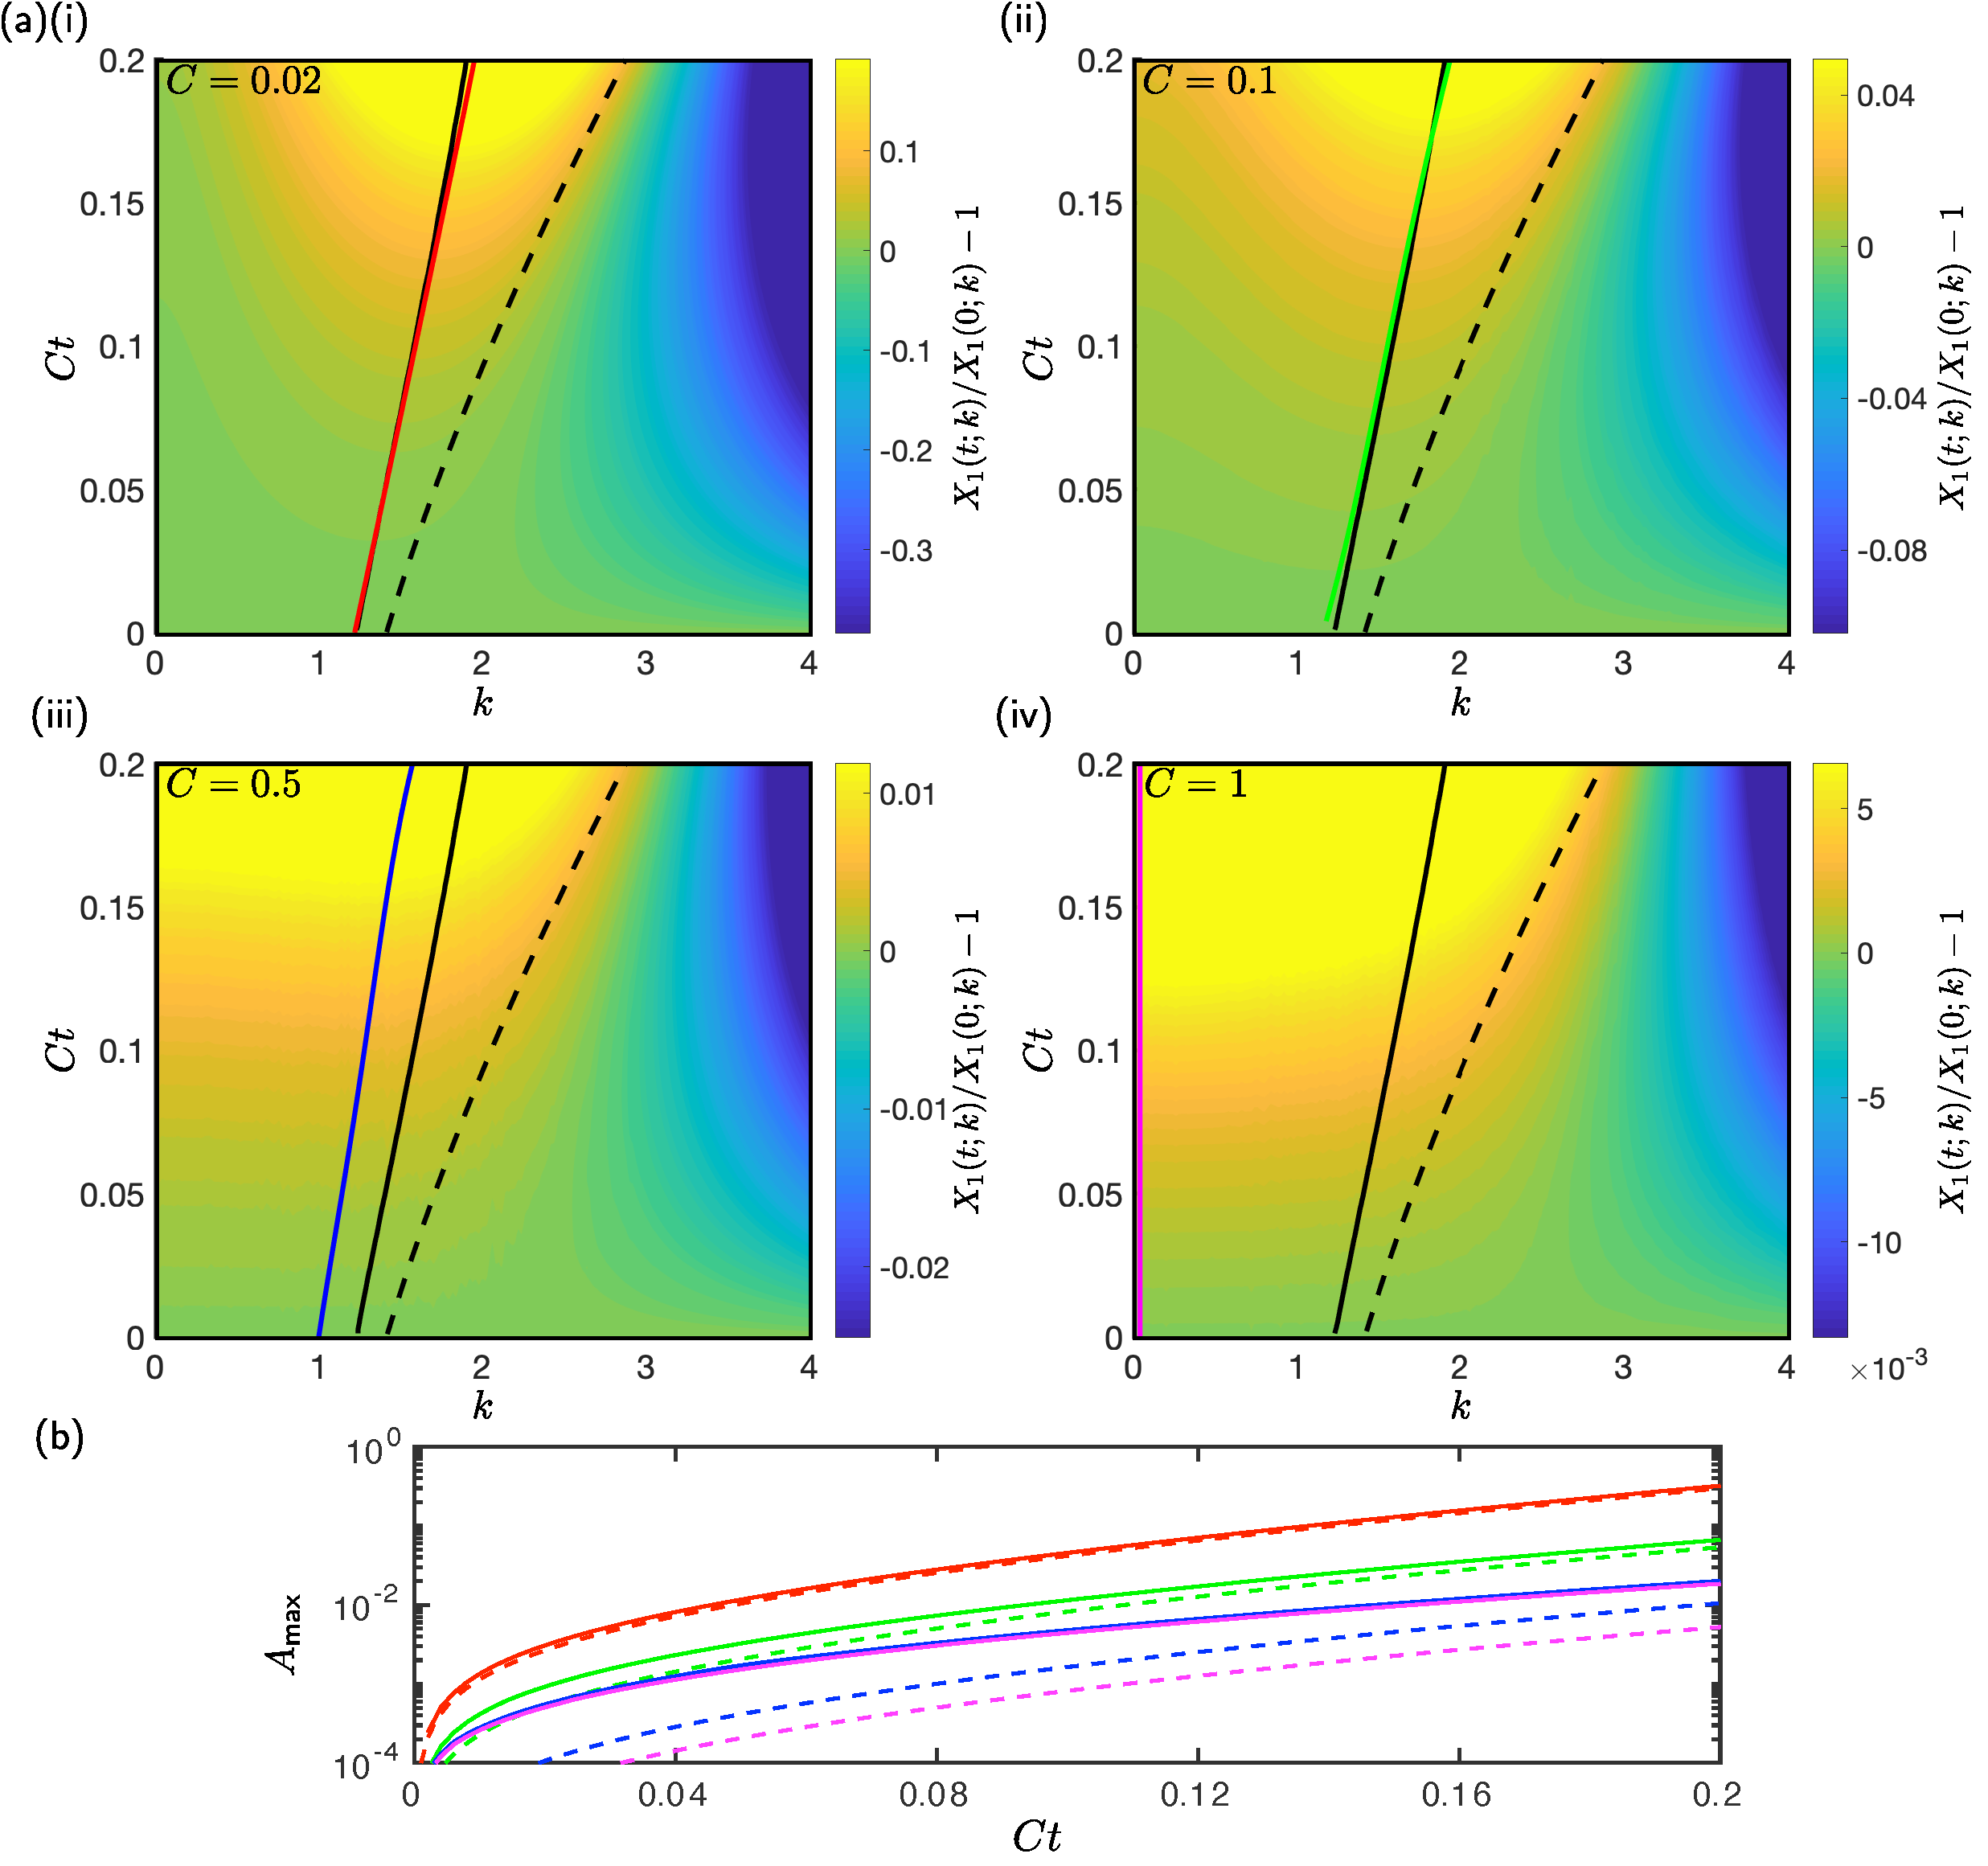
\includegraphics[width = 0.95\textwidth]{contour_plots_various_C}
\caption{Contour plots of mode decay/growth $x_1(t)- 1$: the colour along a vertical line through $k = k_0$ describes the evolution of the perturbation with wavenumber $k_0$ according to the colourbar (note that each colourbar is different, and the colours are saturated to ensure that $0$ has same colour in each plot). The coloured curve (red in (i), green in (ii), blue in (iii), and pink in (iv)) in each plot indicates $k_{\text{max}}$, the mode that has grown the most at each instant of time. The black solid curve indicates the prediction of the quasistatic theory, and the black dashed curve indicates the prediction of the quasistatic theory for small deformations. Results are shown for four different condensation rates are shown as indicated in the top left corner of each plot. (b) Instantaneous maximal displacement, $A_{\text{max}}$ for each of the contour plots in (a). The colours corresponds to those in (a). Also plotted as dashed lines are the corresponding quasistatic approximations to $A_{\text{max}}$.}\label{fig:InstabilityChapter:TimeDepBaseState:contours_k_t_space}
\end{figure}

In Figure~\ref{fig:InstabilityChapter:TimeDepBaseState:FullNumericsTraces} we show the growth of numerically obtained amplitudes $x_1$ for different wavenumbers $k$ and condensation rates $C$.  There are three main qualitative similarities with the quasistatic case described in \S\ref{S:InstabilityChapter:WithCondensation:FrozenTime}. Firstly, modes with small wavenumbers initially grow, and while their growth rate increases, it does so more slowly as time progress (Figure~\ref{fig:InstabilityChapter:TimeDepBaseState:FullNumericsTraces}(a)). Secondly, modes that initially decay start to grow at a finite time and may overtake smaller wavenumber modes (Figure~\ref{fig:InstabilityChapter:TimeDepBaseState:FullNumericsTraces}(b),(c)). Finally, modes with large wavenumbers do not spend enough time in the unstable band to be able to overtake smaller wavenumber modes during the simulation period (Figure~\ref{fig:InstabilityChapter:TimeDepBaseState:FullNumericsTraces}(d)). These observations can be seen for a broader range of wavenumbers $k$ in the contour plots of displacement in Figure~\ref{fig:InstabilityChapter:TimeDepBaseState:contours_k_t_space}, which are generated by numerically solving the equations~\eqref{E:InstabilityChapter:WithCondensation:LinearizedEquations:PDEs1}--\eqref{E:InstabilityChapter:WithCondensation:LinearizedEquations:kinematic} for 200 values of $k$ between $k = 0.02$ and $k = 4$.

However, there are two key differences between the numerical solutions to~\eqref{E:InstabilityChapter:WithCondensation:LinearizedEquations:PDEs1}--\eqref{E:InstabilityChapter:WithCondensation:LinearizedEquations:kinematic} and the quasistatic case of \S\ref{S:InstabilityChapter:WithCondensation:FrozenTime}. Firstly, condensation driven dynamics in the base state enhance the growth rate of perturbations, indicated by the fact that the displacement in numerical solutions is always larger than the corresponding quasistatic approximation. Secondly, the dynamics lengthen the band of unstable modes; in particular, some modes, that initially decay under the quasistatic approximation, grow at early times in the full numerics (compare, for example the $C =0.5$ and $C = 1$ curves in Figure~\ref{fig:InstabilityChapter:TimeDepBaseState:FullNumericsTraces}(b) with the corresponding quasistatic results). These two effects are more pronounced for the largest values of the condensation rate, $C$, as expected.

%how does different wavenumbers change this picture
 At small wavenumbers (Figure~\ref{fig:InstabilityChapter:TimeDepBaseState:FullNumericsTraces}(a)), the numerical solutions (plotted against $Ct$) are almost indistinguishable, suggesting that the growth of the perturbation is controlled primarily by dynamic effects in the base state in this case.
However, at relatively large wavenumbers (Figure~\ref{fig:InstabilityChapter:TimeDepBaseState:FullNumericsTraces}(c)), results barely deviate from the quasistatic prediction, suggesting that the competing-curvature mechanism with a time-dependent volume primarily controls the dynamics, in this case.


The mode with the largest amplitude, denoted $k_{\text{max}}(t)$, and its associated amplitude $A_{\text{max}}(t)$ are time dependent (Figure~\ref{fig:InstabilityChapter:TimeDepBaseState:contours_k_t_space}).
As expected, when the condensation is slow, $k_{\text{max}}$ and $A_{\text{max}}$ are indistinguishable from the quasi-static result (Figure~\ref{fig:InstabilityChapter:TimeDepBaseState:contours_k_t_space}(a)(i)--(ii)). For intermediate condensation rates (Figure~\ref{fig:InstabilityChapter:TimeDepBaseState:contours_k_t_space}(a)(iii)), $k_{\text{max}}(t)$ is shifted towards lower wavenumbers, and the amplitude $A_{\text{max}}$ is enhanced, indicating that condensation driven dynamics of the base state tend to preferentially enhance smaller wavenumber (longer wavelength) modes. (Note that $A_{\text{max}}$ is lower for higher condensation rates when plotted against $Ct$, as in Figure~\ref{fig:InstabilityChapter:TimeDepBaseState:contours_k_t_space}(b), simply because modes have less time to grow -- however, they do show the biggest derivation from the quasistatic theory.) Finally, when condensation is fast, the base state dynamics dominate over the competing curvature instability  -- the mode with the longest wavelength has the largest amplitude (the pink curve in (Figure~\ref{fig:InstabilityChapter:TimeDepBaseState:contours_k_t_space}(a)(iv) corresponds to $k = 0.02$, the smallest wavenumber used to generate the contour plots). For high condensation rates, the maximum amplitude is significantly larger than the corresponding quasistatic prediction  (Figure~\ref{fig:InstabilityChapter:TimeDepBaseState:contours_k_t_space}(b)).

Intuitively, the results described in this section make sense: when liquid is being added to the configuration, the base state is advancing with a flat interface (an infinitely long wavelength), and  those modes which are most coherent (i.e.~have a small wavenumber) will be amplified preferentially.

\section{Summary}
In this Chapter, we set out to understand the periodic pattern that is observed in experiments in which liquid condenses into deformable microchannels. In doing so, we identified a novel instability mechanism that is driven by a competition between interfacial curvatures in the liquid and mediated by the elasticity of the channel in response to liquid pressure. Unlike the similar Al-Housseiny instability, driven by competing interfacial curvatures in liquid confined to a rigid channel, this bendo-capillary instability is theoretically possible in the same channel for both wetting and non-wetting liquids.

We studied this mechanism in detail by considering a simple system that may be susceptible to the instability. For simplicity, we assumed a single meniscus and walls that extend infinitely in the in-plane direction.

We first considered the case of zero condensation, $C = 0$. By performing a linear stability analysis of its equilibrium configurations, we identified that the system is unstable to perturbations of a sufficiently small wavenumber. The linearized equations elucidate the two main ways that the elastic case differs from the rigid (Al-Housseiny) case in two important ways: the bulk channel elasticity is set by the liquid pressure, and the channel responds to the perturbation in a way that tends to enhance the difference between the in-plane and transverse curvatures, increasing the range of unstable wavenumbers. The growth rate of the fastest growing mode is highly sensitive to the amount of liquid within the channel (parametrized by the cross-sectional volume $V$); in particular, we identified that the growth rate $\sigma \sim V^7$ in the case of small deformations and negligible in-plane bending.

In the final section, we analyzed how a non-zero condensation rate affects the mode selection problem. A non-zero condensation rate introduces two variations to the elastocapillary competing-curvature mechanism:  the problem now has a time-dependent volume, and the potential for condensation driven dynamics in the (time-dependent) base state. Numerical solutions of the equations linearized about the base state demonstrated how the modes that initially grow can be overtaken by initially decaying modes, ultimately reaching the non-linear regime earlier. This overtaking behaviour was also predicted analytically with a quasistatic approximation, in which the condensation rate enters via the liquid volume only. Finally, we saw how condensation driven dynamics in the base state result in faster growth of perturbations compared to the quasistatic case, and that modes with smaller wavenumbers are enhanced preferentially.

Ultimately, we expect that the pattern observed at late times will correspond to the mode that is first to reach the non-linear regime, and so the instability refinement we observed will not continue indefinitely. In this sense, the results of the mode selection problem are not able to predict the wavelength that would be observed in practice, but should give a reasonable order of magnitude estimate. In the condensation experiments which originally motivated this study, condensation is very slow ($C \approx 10^{-5}$), and thus condensation driven base state dynamics are unimportant. The quasi-static scaling for the largest wavenumber derived in \S\ref{S:InstabilityChapter:Scaling} should therefore give a order of magnitude estimate for a model prediction of experimentally observed wavelength. Using values from~\cite{Seemann2011JPhysCondMat}, we find that $\nu \approx -12$ and $\aspect \approx -0.38$ in these experiments; the wavelength of approximately $200~\si{\micro \meter}$ that is observed experimentally (see Figure~\ref{fig:InstabilityChapter:Intro:ExptSnapshots}) agrees in its order of magnitude with the scaling result~\eqref{E:InstabilityChapter:Scaling:CriticalWavenumber}, which predicts a wavelength of $370~\si{\micro \meter}$ when the channel is half full, $V = 0.5$. (Note that smaller values of $V$ result in predictions of longer wavelengths, but for $V \approx \mathcal{O}(1)$, these are of the correct order of magnitude; for example with $V = 0.1$, the scaling argument predicts a wavelength of $4~\si{\milli \meter}$.) A more detailed model of the condensation experiments requires consideration of the interaction between neighbouring channels, which appear to undergo the instability simultaneously; this provides motivation for the next chapter, in which we study the interaction between neighbouring channels, each of which would undergo bendotaxis in isolation.

\begin{subappendices}
%\addcontentsline{toc}{section}{Appendices}
\renewcommand{\thesection}{\Alph{section}}
%\appendix
\section{Small deformation asymptotics}\label{A:InstabilityChapter:SmallDeformationAsymptotics}
In this appendix, we describe an asymptotic analysis of the equations describing a periodic perturbation to an equilibrium configuration (equations~\eqref{E:InstabilityChapter:SlowCondensation:Periodic:ODEwet}--\eqref{E:InstabilityChapter:SlowCondensation:Periodic:kinematic}) in the limit of small deformations of the equilibrium configuration, $\epsilon = |\nu| V^4 \ll 1$. In particular, we aim to describe the leading order behaviour of the growth rate $\sigma$ of these perturbations. Note that for simplicity, we consider only wetting configurations here ($\nu >0$) but the analysis is largely similar for non-wetting configurations ($\nu < 0$).

\subsection{Governing equations}\label{A:S:SmallDef:GovEq}
Recall from \S\ref{S:InstabilityChapter:BaseState:Equilibria} that, for $\epsilon \ll 1$, the equilibrium configuration has
\begin{equation}\label{A:E:SmallDeformation:Equations:Asymptotic_x0_to_V}
 x_0 = V\left[1 + \frac{\epsilon}{20}  + \mathcal{O}(\epsilon^2)\right],
\end{equation}
\begin{equation}\label{A:E:SmallDeformation:Equations:Asymptotic_channel_shape}
h_e(x) = 1 + \epsilon\psi \left(\frac{x}{V}\right) + \mathcal{O}(\epsilon^2),\qquad \psi(s) = \frac{-1}{8} + \frac{1}{24}\left[4(1-s) - (1-s)^4\right].
\end{equation}

Before we can proceed with an asymptotic expansion, we need to determine the size of the terms in which the wavenumber $k$ appears. We are primarily interested in those wavenumbers in which the destabilizing transverse and stabilizing in-plane curvature contributions (the terms on the right hand side of~\eqref{E:InstabilityChapter:SlowCondensation:Periodic:pressure_bc}) are comparable. We therefore introduce a scaled wavenumber
\begin{equation}\label{E:Chapter6:SmallDeformation:RescaledProblem:Wavenumber}
k = \left(\frac{\nu V^3}{\aspect}\right)^{1/2} \K,
\end{equation}
which is motivated by the scaling for $k$ we obtained in the scaling argument. We anticipate the majority of the bending deformation occurs in the wet region $0 < x < x_0 = V + \mathcal{O}(\epsilon)$, and introduce the rescaled spatial variable $X = x/V$ to reflect this.

After inserting~\eqref{E:Chapter6:SmallDeformation:RescaledProblem:Wavenumber} and the scaled variable $X$ into the BVP~\eqref{E:InstabilityChapter:SlowCondensation:Periodic:ODEwet}--\eqref{E:InstabilityChapter:SlowCondensation:Periodic:kinematic}, the parameter
\begin{equation}\label{AE:InstabilityChapter:SmallDeformation:RescaledProblem:OtherSmallPar}
\param= \frac{\nu V^5}{|\aspect|} \gg \epsilon
\end{equation}
appears naturally. The parameter $\param$ describes the ratio between bending energies in the in-plane and transverse directions (see \S\ref{S:InstabilityChapter:NoCondensation:SmallDeformations}). The requirement that $\param \gg \epsilon$ ensures that our use of lubrication theory is valid.

We consider the behaviour in the limit $\param \to 0$, which corresponds to relatively small in-plane bending deformations, compared to transverse bending deformations. We expect that the majority of the bending of the dry region occurs in the in-plane direction, so for $\param \ll 1$, the bending of the dry region is not significant. 

We also rescale the perturbed channel shape $H$ and pressure $P$ with $\nu V^3$ to reflect the leading order behaviour -- a shearing force of magnitude $\nu$ applied over a length equal to the magnitude of the perturbation (the shear is the third derivative of the channel deformation, which combined with the length rescaling is responsible for the $V^3$).

After inserting~\eqref{A:E:SmallDeformation:Equations:Asymptotic_x0_to_V} and~\eqref{A:E:SmallDeformation:Equations:Asymptotic_channel_shape} into BVP~\eqref{E:InstabilityChapter:SlowCondensation:Periodic:ODEwet}--\eqref{E:InstabilityChapter:SlowCondensation:Periodic:kinematic}, the problem for
\begin{equation}
G(X) = \frac{H(X)}{\nu V^3}, \qquad Q(X) = \frac{P(X)}{\nu V^3}
\end{equation}
and $\sigma$ reads, correct to $\mathcal{O}\left(\epsilon^2\right)$:
\begin{align}
3\epsilon V^2 \sigma G &= \left(1 + 2\epsilon \psi\right)\left[\epsilon\dd{\psi}{X} \dd{Q}{X} + \left(1 + \epsilon \psi\right)\left(\dd{^2 Q}{X^2} -\param K^2 Q\right)\right] & &0 < X < 1,\label{A:E:Chapter6:SmallDef:BVP:ODEwet}\\
0 &= Q & &1 < X < \frac{1}{V},\label{A:E:Chapter6:SmallDef:BVP:ODEdry}\\
Q &= \dd{^4 G}{X^4} - 2\param K^2 \dd{^2 G}{X^2} +\param K^4 G & &0 < X<\frac{1}{V},\label{A:E:Chapter6:state_BVP:pressure2shape}
\end{align}
with boundary conditions
\begin{align}
G &= 0 = \dd{G}{X} = \dd{Q}{X} & &\text{at}~X = 0,\label{A:E:Chapter6:SmallDef:BVP:BC_at_0}\\
Q + \frac{\epsilon V}{20}\ddp{Q}{X} &= \epsilon\left(\dd{\psi}{X} + G + K^2\right)  & &\text{at}~X= 1,\label{A:E:Chapter6:SmallDef:BVP:pressure_bc}\\
\dd{^2 G}{X^2} -\param \poisson K^2 G &= 0 = \dd{^3 G}{X^3} - (2-\poisson)\param K^2 \dd{G}{X} & &\text{at}~X = \frac{1}{V},\label{A:E:Chapter6:SmallDef:BVP:BC_at_1}
\end{align}
\begin{align}\label{A:E:Chapter6:SmallDef:BVP:jump_conds}
\left[G\right]_-^+= \left[\dd{G}{x}\right]_-^+ = \left[\dd{^2G}{X^2} + \frac{\epsilon V}{20}\dd{^3 G}{X^3}\right]_-^+&= 0, \\
\left[\dd{^3 G}{X^3} + \frac{\epsilon V}{20}\dd{^4 G}{X^4}\right]_-^+ &= 1 - \epsilon \psi(1).
\end{align}
Here the jump applies across the (unperturbed) contact line $X = 1$.The growth rate $\sigma$ satisfies
\begin{equation}\label{A:E:Chapter6:SmallDef:BVP:kinematic}
3V^2\sigma = -\left[1 + 2\epsilon \psi(1)\right]\left[\dd{Q}{X} + \frac{\epsilon V}{20}\dd{^2 Q}{X^2}\right]_{X = 1}.
\end{equation}

\subsection{Bivariate expansion}
We analyse the asymptotic structure of the rescaled problem~\eqref{A:E:Chapter6:SmallDef:BVP:ODEwet}--\eqref{A:E:Chapter6:SmallDef:BVP:kinematic} by posing the bivariate asymptotic expansion
\begin{align}
G &=  G_{0,0} + \param G_{1,0} + \epsilon G_{0,1} +  \param^2 G_{2,0} + \param \epsilon G_{1,1} + \epsilon^2 G_{0,2} + \dots,\label{A:E:Chapter6:SmallDeformation:Expansion:ExpansionH} \\
Q &=  Q_{0,0} + \param Q_{1,0} + \epsilon Q_{0,1} +  \param^2 Q_{2,0} + \param \epsilon Q_{1,1} + \epsilon^2 Q_{0,2} + \dots,\label{A:E:Chapter6:SmallDeformation:Expansion:ExpansionP} \\
\sigma &= \sigma_{0,0} + \param \sigma_{1,0} + \epsilon \sigma_{0,1} +  \param^2 \sigma_{2,0} + \param \epsilon \sigma_{1,1} + \epsilon^2 \sigma_{0,2} + \dots. \label{A:E:Chapter6:SmallDeformation:Expansion:ExpansionSigma}
\end{align}
The particular hierarchy of problems that emerges depends on the relative sizes of $\epsilon$ and $\param \gg \epsilon$. Clearly, if $\epsilon \ll \param^2$, terms like $G_{2,0}$ will dominate $G_{0,1}$ while if $\param^2 \ll \epsilon$ it will be the other way around. We therefore consider the distinguished limit $\epsilon \sim \param^2$, writing $\epsilon = \beta \param^2$ with $\beta \sim \mathcal{O}(1)$. (In any case, the first and leading order problems are independent of the precise details of the relative sizes of $\epsilon$ and $\param \gg \epsilon$.)

We therefore rewrite the expansion as
\begin{align}
G &= G_0 + \param G_1 + \param^2 G_2 + \param^3 G_3 + \mathcal{O}\left(\param^4\right),\\
Q &= Q_0 + \param Q_1 + \param^2 Q_2 + \param^3 Q_3 + \mathcal{O}\left(\param^4\right),\label{A:E:SmallDef:Expansion:ExpansionQ}\\
\sigma &= \sigma_0 + \param \sigma_1 + \param^2 \sigma_2 + \param^3 \sigma_3 + \mathcal{O}\left(\param^4\right).
\end{align}
We do not include any terms that are $\mathcal{O}\left(\param^4\right) = \mathcal{O}\left(\epsilon^2\right)$ because the rescaled problem~\eqref{A:E:Chapter6:SmallDef:BVP:ODEwet}--\eqref{A:E:Chapter6:SmallDef:BVP:kinematic} is only correct to $\mathcal{O}\left(\epsilon^2\right)$.

\subsubsection{Leading and first order problem}
The leading order problem is given by
\begin{align}
0&= \dd{^2Q_0}{X^2} & &0 < X<1,\label{A:E:Chapter6:SmallDef:Expansion:0thOrder:ODEwet}\\
0&= Q_0  & &1 < X< \frac{1}{V},\\
Q_0 &= \dd{^4 G_0}{X^4} & & 0 < X < \frac{1}{V},
\end{align}
\begin{align}
G_0 &= 0 = \dd{G_0}{X}= \dd{Q_0}{X} & &\text{at}~X = 0,\label{A:E:Chapter6:SmallDef:Expansion:0thOrder:x0bc}\\
Q_0 &=0 & &\text{at}~X = 1,\label{A:E:Chapter6:SmallDef:Expansion:0thOrder:pressurebc}\\
\dd{^2 G_0}{X^2} &=0 = \dd{^3 G_0}{X^3} & &\text{at}~X = \frac{1}{V},
\end{align}
\begin{equation}
\left[G_0\right]_-^+ =0 = \left[\dd{G_0}{X}\right]_-^+ = \left[\dd{^2 G_0}{X^2}\right]_-^+, \quad  \left[\dd{^3 G_0}{X^3}\right]_-^+ = 1
\end{equation}
\begin{equation}\label{A:E:Chapter6:SmallDef:Expansion:0thOrder:kinematic}
3V^2 \sigma_0 = -\left.\dd{Q_0}{X}\right|_{X=1}
\end{equation}
From~\eqref{A:E:Chapter6:SmallDef:Expansion:0thOrder:ODEwet},  the pressure $Q_0$ is a linear function of $X$. However, from~\eqref{A:E:Chapter6:SmallDef:Expansion:0thOrder:x0bc}--\eqref{A:E:Chapter6:SmallDef:Expansion:0thOrder:pressurebc}, this linear function has no slope and passes through zero; we therefore have $Q_0 = 0$, and from~\eqref{A:E:Chapter6:SmallDef:Expansion:0thOrder:kinematic} $\sigma_0 = 0$. The solution to~\eqref{A:E:Chapter6:SmallDef:Expansion:0thOrder:ODEwet}--\eqref{A:E:Chapter6:SmallDef:Expansion:0thOrder:kinematic} for the channel shape is
\begin{equation}\label{A:E:Chapter6:SmallDef:Expansion:0thOrder:shape_sol}
G_0 = \begin{cases}
-\frac{\X^2}{6}\left(3-X\right) & 0 < X < 1,\\
-\frac{1}{6}\left(X-1\right) & 1< X < 1/V.
\end{cases}
\end{equation}

The first order problem is similar. Again, we get no pressure contribution, $Q_1 = 0$ (the equations for $Q_1$ are identical to those for $Q_0$) and thus $\sigma_1 = 0$. The shape contribution $G_1$ is non-trivial, but is not required for the determination of the leading order behaviour for $\sigma$, and we therefore do not state it here. We note, however, that the Poisson's ratio $\poisson$ first appears in this term, highlighting the lower order contribution of the dry regions. (For a balance between $\epsilon$ and $\param$ other than $\epsilon \sim \param^2$, as assumed here, the  statements in this paragraph remain true.)
%%%%%%%%%%%%%%%%%%%%%
%%% First order problem %%%%%%%

%\subsubsection{First order problem}
%Using the solutions \red{ref}, the first order problem is very similar
%\begin{align}
%0&= \ddp{^2 Q_1}{X^2}  & &0 < X<1,\label{A:E:Chapter6:SmallDef:Expansion:1stOrder:ODEwet}\\
%0 &= Q_1 & &1 < X< \frac{1}{V},\\
%Q_1 &= \dd{^4 G_1}{X^4}  - 2K^2 \dd{^2 G_0}{X^2}& & 0 < X < \frac{1}{V},
%\end{align}
%\begin{align}
%G_1 &= 0 = \dd{G_1}{X}= \dd{Q_1}{X} & &\text{at}~X = 0,\\
%Q_1 &=0 & &\text{at}~X = 1,\\
%\dd{^2 G_1}{X^2} - \poisson K^2 G_0 &=0 = \dd{^3 G_1}{X^3} - (2- \poisson )K^2 \dd{G_0}{X}& &\text{at}~X = \frac{1}{V},
%\end{align}
%\begin{equation}
%\left[G_1\right]_-^+ =0 = \left[\dd{G_1}{X}\right]_-^+ = \left[\dd{^2 G_1}{X^2}\right]_-^+ =  \left[\dd{^3 G_1}{X^3}\right]_-^+
%\end{equation}
%\begin{equation}\label{A:E:Chapter6:SmallDef:Expansion:1stOrder:kinematic}
%3V^2 \sigma_1 = -\left.\dd{Q_1}{X}\right|_{X=1}.
%\end{equation}

\subsubsection{Higher order problems}
The  $\mathcal{O}(\param^2)$ problem may be expressed simply be exploiting the  $\mathcal{O}(1)$ and $\mathcal{O}(\param)$ problems. We give only this simplified form here:
\begin{align}
 \dd{^2 Q_2}{X^2}&=0 & &0 < X<1,\\
Q_2 &= 0 & &1 < X< \frac{1}{V},\\
Q_2 &= \dd{^4 G_2}{X^4} - 2K^2\dd{G_1}{X^2}+ K^4 G_0 & & 0 < X < \frac{1}{V},
\end{align}
\begin{align}
G_2 &= 0 = \dd{G_2}{X}= \dd{Q_2}{X} & &\text{at}~X = 0,\\
Q_2 &=G_0+ K^2+ \dd{\psi}{X} & &\text{at}~X = 1,\label{A:E:Chapter6:SmallDef:Expansion:2ndOrder:PressureBC}\\
\dd{^2 G_2}{X^2} - \poisson K^2 G_1 &=0 = \dd{^3 G_0}{X^3}  - (2- \poisson)K^2 \dd{G_1}{X}& &\text{at}~X = \frac{1}{V},
\end{align}
\begin{equation}
\left[G_2\right]_-^+ =0 = \left[\dd{G_2}{X}\right]_-^+ = \left[\dd{^2 G_2}{X^2} + \frac{\beta V}{20}\dd{^3G_0}{X^3}\right]_-^+, = \left[\dd{^3 G_2}{X^3} + \frac{\beta V}{20}\dd{^4 G_0}{X^4}\right]_-^+
\end{equation}
\begin{equation}
3V^2 \sigma_2 = -\left.\dd{Q_2}{X}\right|_{X=1}.
\end{equation}
Crucially, the boundary condition~\eqref{A:E:Chapter6:SmallDef:Expansion:2ndOrder:PressureBC} is inhomogeneous, in contrast to the corresponding boundary condition for the lower order problem. We therefore find the first non-zero pressure term in~\eqref{A:E:SmallDef:Expansion:ExpansionQ} to be
\begin{equation}\label{A:E:Chapter6:SmallDef:Expansion:2ndOrder:solQ2}
Q_2 = \begin{cases}
K^2 - \frac{1}{2} & 0 <X  < 1,\\
0 & 1 < X < 1/V,
\end{cases}
\end{equation}
where we have used $G_0$, from~\eqref{A:E:Chapter6:SmallDef:Expansion:0thOrder:shape_sol}, to obtain $Q_2$. (Note that for a relationship other than $\epsilon\sim \param^2$, the boundary condition~\eqref{A:E:Chapter6:SmallDef:Expansion:2ndOrder:PressureBC} would be unchanged because the shape contributions at higher order all take the same value at $ X= 1$.) This leading order pressure contribution is constant in the liquid and thus again offers no contribution to the growth rate, hence $\sigma_2 = 0$.

To obtain a non-zero term in the expansion for $\sigma$ we must proceed to $\mathcal{O}(\param^3)$, where we find that
\begin{align}
 \dd{^2 Q_3}{X^2} - K^2 Q_2 &= 0 & &0 < X<1,\label{A:E:Chapter6:SmallDef:Expansion:3ndOrder:odewet}\\
Q_3 &= 0 & &1 < X< \frac{1}{V},\\
Q_3 &= \dd{^4 G_3}{X^4} - 2K^2\dd{G_2}{X^2}+ K^4 G_1 & & 0 < X < \frac{1}{V},
\end{align}
\begin{align}
G_3 &= 0 = \dd{G_3}{X}= \dd{Q_3}{X} & &\text{at}~X = 0,\label{A:E:Chapter6:SmallDef:Expansion:3ndOrder:x0bc}\\
Q_3 &=\beta G_1 & &\text{at}~X = 1,\label{A:E:Chapter6:SmallDef:Expansion:3ndOrder:PressureBC}\\
\dd{^2 G_2}{X^2} - \poisson K^2 G_1 &=0 = \dd{^3 G_0}{X^3}  - (2- \poisson)K^2 \dd{G_1}{X}& &\text{at}~X = \frac{1}{V},
\end{align}
\begin{equation}
\left[G_3\right]_-^+ =0 = \left[\dd{G_3}{X}\right]_-^+ = \left[\dd{^2 G_3}{X^2} + \frac{\beta V}{20}\dd{^3G_1}{X^3}\right]_-^+, = \left[\dd{^3 G_3}{X^3} + \frac{\beta V}{20}\dd{^4 G_1}{X^4}\right]_-^+
\end{equation}
\begin{equation}\label{A:E:Chapter6:SmallDef:Expansion:3ndOrder:kinematic}
3V^2 \sigma_3 = -\left.\dd{Q_3}{X}\right|_{X=1}.
\end{equation}
From~\eqref{A:E:Chapter6:SmallDef:Expansion:3ndOrder:odewet} and~\eqref{A:E:Chapter6:SmallDef:Expansion:3ndOrder:x0bc}, we find that
\begin{equation}\label{A:E:Chapter6:SmallDef:Expansion:3ndOrder:solutionQ3}
\dd{Q_3}{X} = K^2 Q_2 X \qquad 0 < X < 1.
\end{equation}
Inserting~\eqref{A:E:Chapter6:SmallDef:Expansion:3ndOrder:solutionQ3} into~\eqref{A:E:Chapter6:SmallDef:Expansion:3ndOrder:kinematic}, and using~\eqref{A:E:Chapter6:SmallDef:Expansion:2ndOrder:solQ2} gives
\begin{equation}\label{A:E:Chapter6:SmallDef:Expansion:3ndOrder:solutionsigma3}
\sigma_3  = -\frac{K^2}{6V^2}\left(2K^2 - 1\right).
\end{equation}
This is the leading order term in the expansion~\eqref{A:E:Chapter6:SmallDeformation:Expansion:ExpansionSigma} for $\sigma$.

Undoing the various variable changes introduced in Appendix~\ref{A:S:SmallDef:GovEq}, the result~\eqref{A:E:Chapter6:SmallDef:Expansion:3ndOrder:solutionsigma3} gives
\begin{equation}\label{AE:InstabilityChapter:SmallDeformation:ThirdOrder:SigmaSolution}
\sigma\sim \frac{\nu^2 V^7}{a}F\left(\frac{k}{k_c}\right)
\end{equation}
where
\begin{equation}\label{AE:InstabilityChapter:SmallDeformation:ThirdOrder:SigmaSolutionParticulars}
F(\xi) = -\frac{\xi^2}{6}\left(2\xi^2 -1\right), \qquad k_c = \left(\frac{\nu V^3}{a}\right)^{1/2}.
\end{equation}
Note that~\eqref{AE:InstabilityChapter:SmallDeformation:ThirdOrder:SigmaSolution} agrees with the scaling argument presented in \S\ref{S:InstabilityChapter:Scaling}.

\section{Details of numerical scheme}\label{A:Chapter6:Numerics}
In this appendix, we give details of the numerical scheme used to solve the system of PDEs and boundary conditions~\eqref{E:InstabilityChapter:BaseState:FlatInterface:PDEwet}--\eqref{E:InstabilityChapter:BaseState:FlatInterface:kinematicbc} and~\eqref{E:InstabilityChapter:WithCondensation:LinearizedEquations:PDEs1}--\eqref{E:InstabilityChapter:WithCondensation:LinearizedEquations:kinematic} for $h_0, h_1, p_0,p_1, x_0, x_1$ that describe both the dynamic evolution of the base state, and the growth of periodic perturbations to it. Note that the equations describing the evolution of $h_0, p_0,x_0$ can be solved without also solving for $h_1, p_1,x_1$ (but not the other way around) so this section also describes the scheme used to numerically solve the PDEs~\eqref{E:InstabilityChapter:BaseState:FlatInterface:PDEwet}--\eqref{E:InstabilityChapter:BaseState:FlatInterface:kinematicbc} for $h_0, p_0,x_0$ in isolation.

\subsection{Isolating the wet region}
We begin by reducing the problem to be solved to one defined only on the wet region, $0 < x < x_0(t)$. This is possible because both the base state channel shape $h_0$, and the perturbation to it, $h_1$, can be expressed analytically in the the dry region ($x_0 < x < 1$) in terms of the channel shape at $x = x_0$.

Explicitly, we integrate~\eqref{E:InstabilityChapter:BaseState:FlatInterface:PDEwet}--\eqref{E:InstabilityChapter:BaseState:FlatInterface:pressure2shape}
and~\eqref{E:InstabilityChapter:WithCondensation:LinearizedEquations:PDEs2}--\eqref{E:InstabilityChapter:WithCondensation:LinearizedEquations:Pressure2Shape} directly to obtain
\begin{align}
h_0 &= C_1 x + C_1 & & x_0(t) < x < 1,\label{E:InstabilityChapter:WithCondensation:Numerics:dry_solution0}\\
h_1 &= (D_1 x + D_2)\exp(kx) + (D_3 x + D_4)\exp(-kx) & & x_0(t) < x < 1,\label{E:InstabilityChapter:WithCondensation:Numerics:dry_solution1}
\end{align}
where the $C_i(t), D_i(t), i = 1,\dots, 4$ are constants of integration.

Inserting~\eqref{E:InstabilityChapter:WithCondensation:Numerics:dry_solution1} into the two boundary conditions~\eqref{E:InstabilityChapter:WithCondensation:LinearizedEquations:bc_x=1} and the four continuity  conditions~\eqref{E:InstabilityChapter:WithCondensation:LinearizedEquations:JumpConditions} allows us to express the $C_i, i = 1,\dots,4$ in terms of the channel shape at $x = x_0$ provided that two constraints on the wall shape of the form
\begin{equation}\label{E:InstabilityChapter:WithCondensation:Numerics:effbc}
\ddp{^3 h_1}{x^3} = \psi_1 \ddp{h_1}{x} + \psi_2 h_1 + \psi_3 x_1, \quad \ddp{^2 h_1}{x^2} = \phi_1 \ddp{h_1}{x} + \phi_2 h_1 + \phi_3 x_1 \quad \text{at}~x  = x_0
\end{equation}
hold. Here $\psi_i, \phi_i, i = 1,2,3$ are (known) functions of $k, \eta, x_0,$ and $\nu$. Equations~\eqref{E:InstabilityChapter:WithCondensation:Numerics:effbc} can be thought of as effective boundary conditions, which parametrise the effect of the dry region on the wet region.

The same procedure applied to the base state results in effective boundary conditions
\begin{equation}\label{E:InstabilityChapter:WithCondensation:Numerics:effbc_base_state}
\ddp{^3 h_0}{x^3} = 0= \ddp{^2 h_1}{x^2} \quad\text{at}~x  = x_0.
\end{equation}

With~\eqref{E:InstabilityChapter:WithCondensation:Numerics:effbc} and~\eqref{E:InstabilityChapter:WithCondensation:Numerics:effbc_base_state}, we have a complete system of equations for $h_0$, $h_1$,  $p_0$, $p_1$, $x_0$, and $x_1$ that involves only the drop region. These are the four PDEs~\eqref{E:InstabilityChapter:BaseState:FlatInterface:PDEwet}, \eqref{E:InstabilityChapter:BaseState:FlatInterface:pressure2shape}, \eqref{E:InstabilityChapter:WithCondensation:LinearizedEquations:PDEs1}, \eqref{E:InstabilityChapter:WithCondensation:LinearizedEquations:Pressure2Shape}, the boundary conditions~\eqref{E:InstabilityChapter:BaseState:FlatInterface:bc0}--\eqref{E:InstabilityChapter:BaseState:FlatInterface:jumpbc},
\eqref{E:InstabilityChapter:WithCondensation:LinearizedEquations:bc_x=0}--\eqref{E:InstabilityChapter:WithCondensation:LinearizedEquations:kinematic}, \eqref{E:InstabilityChapter:WithCondensation:Numerics:effbc}--\eqref{E:InstabilityChapter:WithCondensation:Numerics:effbc_base_state} and the kinematic conditions~\eqref{E:InstabilityChapter:BaseState:FlatInterface:kinematicbc} and~\eqref{E:InstabilityChapter:WithCondensation:LinearizedEquations:kinematic}.
\subsection{Transformation to a fixed domain and discretization}
This system of equations is transformed onto a time-independent domain, $0 < s < 1$ using
\begin{equation}\label{E:InstabilityChapter:WithCondensation:Numerics:transformation}
s = \frac{x}{x_0(t)}.
\end{equation}
Since $s$ is time-dependent, the transformation~\eqref{E:InstabilityChapter:WithCondensation:Numerics:transformation} introduces additional advective terms in the system of equations; the time derivatives in the two co-ordinate systems are related by
\begin{equation}\label{E:InstabilityChapter:WithCondensation:Numerics:transformation_space_derivative}
\left(\ddp{}{t}\right)_{x} =\left(\ddp{}{t}\right)_{s} +\frac{s}{x_0(t)}\dd{x_0}{t} \ddp{}{z},
\end{equation}
where $\left(.\right)_{\chi}$ refers to the derivative with  $\chi$ held constant. Spatial derivatives are straightforward, since
\begin{equation}\label{E:InstabilityChapter:WithCondensation:Numerics:transformation_time_derivatives}
\left(\ddp{}{s} \right)_t= \frac{1}{x_0(t)}\left(\ddp{}{s}\right)_t.
\end{equation}
We also introduce
\begin{equation}\label{E:InstabilityChapter:WithCondensation:Numerics:transformation_base_state_shape}
u_0(x,t) = x_0(t)h_0(x,t)
\end{equation}
to allow the base state equations to be expressed in conservative form.

With the transformation~\eqref{E:InstabilityChapter:WithCondensation:Numerics:transformation} and~\eqref{E:InstabilityChapter:WithCondensation:Numerics:transformation_base_state_shape} the PDEs~\eqref{E:InstabilityChapter:BaseState:FlatInterface:PDEwet}, \eqref{E:InstabilityChapter:BaseState:FlatInterface:pressure2shape}, \eqref{E:InstabilityChapter:WithCondensation:LinearizedEquations:PDEs1}, and \eqref{E:InstabilityChapter:WithCondensation:LinearizedEquations:Pressure2Shape}, become
\begin{align}
0& = \ddp{u_0}{t} + \ddp{q_0}{s},\label{A:E:Ch6:Numerics:Transformation:FluxConsEqBaseState}\\
p_0 &= \frac{1}{x_0^4} \ddp{^4 h_0}{s^4},\label{A:E:Ch6:Numerics:Transformation:Pressure2ShapeBaseState}\\
0&= \ddp{h_1}{t} +  \ddp{q_1}{s} +  \frac{1}{3|\nu|} k^2 h_0^3 p_1  + \frac{\dot{x}_0}{x_0}h_1,\label{A:E:Ch6:Numerics:Transformation:FluxConsPerturbation}\\
p_1 &= \frac{1}{x_0^4}\ddp{^4 h_1}{x^4} - \frac{2k^2}{x_0^2} \ddp{^2 h_1}{x^2}  + k^4 h_1.\label{A:E:Ch6:Numerics:Transformation:Pressure2ShapePerturbation}
\end{align}
where
\begin{align}
q_0 & = -\frac{1}{x_0}\left[\frac{1}{3|\nu|}\frac{u_0^3}{x_0^3}\ddp{p_0}{z}  + u_0 z\dd{x_0}{t} \right],\label{A:E:Ch6:Numerics:Transformation:BaseStateFlux}\\
q_1 &= - \frac{1}{x_0}\left[\frac{1}{3|\nu|}\left(\frac{u_0^3}{x_0^3}\ddp{p_1}{s} + 3\frac{u_0^2}{x_0^2} \ddp{p_0}{s}h_1\right) +   h_1 z\dd{x_0}{t} \right],\label{A:E:Ch6:Numerics:Transformation:PerturbationFlux}
\end{align}
play the role of the flux.

The boundary conditions on~\eqref{A:E:Ch6:Numerics:Transformation:FluxConsEqBaseState}--\eqref{A:E:Ch6:Numerics:Transformation:Pressure2ShapePerturbation} are:
\begin{align}
h_0 &= 1, \quad h_1 = \ddp{h_1}{s} = \ddp{p_1}{s} =\ddp{h_0}{s} = \ddp{p_0}{s} = 0 & &\text{at}~s = 0,\label{A:E:Ch6:Numerics:Transformation:clampedBC}\\
p_0 &= \frac{-\nu x_0}{u},\quad
p_1 + \frac{x_1}{x_0} \ddp{p_0}{s} =\frac{\nu}{\h_0^2}\left(\frac{x_1}{x_0^2}\dd{u_0}{s} + h_1\right) + \nu \aspect  k^2 x_1, & &\text{at}~s = 1,
\label{A:E:Ch6:Numerics:Transformation:pressureBC}\\
\ddp{^3 u_0}{s^3} &= 0, \quad \frac{1}{x_0^3}\ddp{^3 h_1}{s^3} = \frac{\psi_1}{x_0} \ddp{h_1}{s} + \psi_2 h_1 + \psi_3 x_1 & &\text{at}~s = 1,\label{A:E:Ch6:Numerics:Transformation:effectiveBC1}\\
\ddp{^2 u_0}{s^2} &= 0, \quad \frac{1}{x_0^2}\ddp{^2 h_1}{s^2} =  \frac{\phi_1}{x_0} \ddp{h_1}{x} + \phi_2 h_1 + \phi_3 x_1 & &\text{at}~s = 1.\label{A:E:Ch6:Numerics:Transformation:effectiveBC2}
\end{align}
The base state meniscus position evolves according to
\begin{equation}\label{A:E:Ch6:Numerics:Transformation:kinematic_x0}
\dd{x_0}{t} =\left. \frac{-1}{3|\nu|}\frac{u_0^2}{x_0^3}\ddp{p_0}{s}\right|_{s = 1}
\end{equation}
and the perturbation to this evolves according to
\begin{equation}\label{A:E:Ch6:Numerics:Transformation:kinematic_x1}
\dd{x_1}{t} =-\frac{1}{3|\nu|}\left.\left[\frac{ u_0^2}{x_0^3} \ddp{p_1}{s} + \frac{x_1}{x_0^4} \ddp{}{s}\left(u_0^2 \ddp{p_0}{s} \right) + \frac{2 u_0}{x_0^2} \ddp{p_0}{s} h_1 \right]\right|_{s=1}.
\end{equation}

We solve the problem~\eqref{A:E:Ch6:Numerics:Transformation:FluxConsEqBaseState}--\eqref{A:E:Ch6:Numerics:Transformation:PerturbationFlux} numerically by discretizing in space: the $s$-domain is divided into a grid of $n$ cells of equal length $\Delta s = 1/n$ with cell centres $s_j = (j - 1/2)\Delta s$ for $j = 1,\dots,n$, and cell edges at $s_{j+1/2} = j\Delta s$ for $j = 0,...n$. $h_0,p_0,h_1$, and $p_1$ approximated at the centre of each cell by $h_0^j, p_0^j, h_1^j$ and $p_1^j$, respectively. The fluxes $q_0$ and $q_1$ are approximated at the edge of the cells using second order centred finite differences of the $h_0^j$ and $h_1^j$.

Two ghost points are introduced at each end of the domain (corresponding to cell centres indexed by $j = -1,0$ and $j = n+1, n+2$, respectively). By approximating $h_0, h_1,p_0$ and $p_1$ appropriately at these points, we implement the boundary conditions~\eqref{A:E:Ch6:Numerics:Transformation:clampedBC}--\eqref{A:E:Ch6:Numerics:Transformation:effectiveBC2}.

The finite difference discretization of~\eqref{A:E:Ch6:Numerics:Transformation:FluxConsEqBaseState} and~\eqref{A:E:Ch6:Numerics:Transformation:FluxConsPerturbation} results in a system of $2n$, ODEs for  $h_0^j(t)$ and $h_1^j(t)$. These ODEs are coupled to the $2n$ algebraic equations that arise from the finite difference discretization of~\eqref{A:E:Ch6:Numerics:Transformation:Pressure2ShapeBaseState} and~\eqref{A:E:Ch6:Numerics:Transformation:Pressure2ShapePerturbation} as well as to the ODEs for $x_0$ and $x_1$ arising from the discretization of~\eqref{A:E:Ch6:Numerics:Transformation:kinematic_x0} and~\eqref{A:E:Ch6:Numerics:Transformation:kinematic_x1}. This system of $4n+2$ differential-algebraic equations are solved using the \texttt{ODE15s} routine implemented in \textsc{matlab}.

\subsection{Initial conditions}
We assume that the initial volume $V_0$ is prescribed and compute the shape, pressure, and meniscus position of the corresponding $C = 0$ equilibrium (see \S\ref{S:InstabilityChapter:BaseState:Equilibria}). These are used as the initial condition on the base state quantities $h_0, p_0$, and $x_0$.

The initial condition for the perturbation requires care. We anticipate that, as in the $C = 0$ case, there will be two modes of growth for the perturbation, one of which displays very high decay rates for all wavenumbers and one of which has a band of unstable wavenumbers. To ensure that the numerics select the branch on which modes grow (corresponding to the $\sigma_2$ branch for the $C = 0$ case, see Figure~\ref{fig:InstabilityChapter:SlowCondensation:GrowthRates}), we use the solution of the quasistatic BVP~\eqref{E:InstabilityChapter:SlowCondensation:Periodic:ODEwet}--\eqref{E:InstabilityChapter:SlowCondensation:Periodic:kinematic} whose growth rate that lies on the correct branch as the initial condition on the shape and pressure of the perturbation.


\end{subappendices}
}


\newcommand{\xrightj}{x_{j}^{+}}
\newcommand{\xleftj}{x_{j}^{-}}
\newcommand{\xrightjj}{x_{j+1}^{+}}
\newcommand{\xleftjj}{x_{j+1}^{-}}
\renewcommand{\xright}[1]{x_{+}^{#1}}
\renewcommand{\xleft}[1]{x_{-}^{#1}}

\newcommand{\xbarj}{\bar{x}_j}
\newcommand{\ellj}{\ell_j}
\newcommand{\xbar}{\bar{x}}
\newcommand{\dtheta}{\left(\theta_{j+1/2} - \theta_{j-1/2}\right)}
\newcommand{\ddeltatheta}{\left(\dot{\theta}_{j+1/2}-\dot{\theta}_{j-1/2}\right)}
\newcommand{\ddeltathetaN}{\left(\dot{\theta}_{j+3/2}-\dot{\theta}_{j+1/2}\right)}
\newcommand{\xbark}[1]{\bar{x}_{#1}}
\newcommand{\ellk}[1]{\ell_{#1}}
\newcommand{\sgn}{\mathrm{sgn}}
\newcommand{\hbrj}[1]{\left(1 + \bar{x}_{#1} \Delta \theta_{#1}\right)}
\newcommand{\dthetaj}{\Delta \theta_j}
\newcommand{\huj}{1 + (\bar{x}_j + \ell_j)\Delta \theta_j}
\newcommand{\hlj}{1 + (\bar{x}_j - \ell_j)\Delta \theta_j}
\newcommand{\geompar}{\mu}
\newcommand{\eps}{\delta}
\newcommand\numberthis{\addtocounter{equation}{1}\tag{\theequation}}
\newcommand{\viscdamp}{C^{\text{d}}}
\renewcommand{\th}{\text{th}}

\DeclarePairedDelimiter\ceil{\lceil}{\rceil}
\DeclarePairedDelimiter\floor{\lfloor}{\rfloor}


\graphicspath{{./Sections/Chapter6_multibody/figures/}}
\chapter{Multibody bendotaxis}\label{Ch:MultibodyBendotaxis}

\section{Introduction}\label{S:Intro}
So far, our focus has been restricted to a single channel. In this chapter, we consider an array of droplet-channel systems, each of which would undergo bendotaxis in isolation; we refer to this as multi-body bendotaxis. Ultimately, we aim to understand how drops in neighbouring channels would affect each other's bendotaxis. Understanding this interaction is relevant not only for self-cleaning surfaces exploiting bendotaxis (which naturally have many neighbouring features on their surface and thus channels in which a droplet may confine itself), but also for the experiments of Figure 5.1 in which droplets are condensed into deformable microchannels; in the previous chapter we described how a bendo-capillary instability may be responsible for wavelength selection in the direction parallel to the channel walls, and in this chapter we seek to understand how the presence of liquid in neighbouring channels might influence its behaviour.

\subsection{Summary of multibody elastocapillary phenomena}
The influence of capillary forces on arrays of pillars and lamellae has been a topic of interest for many years, originally spurred by issues associated with the miniaturization of devices; the down-scaling of components results in an increased surface area to volume ratio and hence a more prominent role for surface forces. \cite{Tanaka1993} verified that it is during the liquid-rinsing step of photo-lithography (a technique relied upon in the manufacture of micro-electromechanical systems, or MEMS) that catastrophic sticking (`stiction') between elements can occur. The surface tension of the rinsing liquid is responsible for stiction, and this process is generally understood at a theoretical level by focussing on a single cantilever beam or a single channel with elastic bounding walls (see for example~\cite{Zhao2003} for a review). In doing so, these models neglect the influence of liquid in neighbouring channels and thus cannot describe how collaborative effects (such as how the deformation of the channel will affect the width of neighbouring channels) influence the aggregation process.

Stiction was originally viewed as a detrimental process since it has been shown to diminish the optical, electrical and mechanical performance of MEMS devices~\citep{DeVolder2013Angewandte}. However, in other settings, elastocapillary self assembly and associated instabilities driving long range order have been successfully exploited to produce novel structures on both the nano and micro-scale. For example, wetting and drying of carbon nanotube forests can increase their packing density~\citep{Chakrapani2004PNAS} or form periodic assemblies \cite[See for example][and references therein]{DeVolder2013Angewandte}, whilst on the micro-scale, surface tension induced aggregation and subsequent collapse can be used to trap colloids~\citep{Pokroy2009Science}.

Mathematical modelling of elastocapillary self assembly experiments such as these often aims to predict the clustering behaviour of high aspect ratio pillars. As with most models, one has to make a trade off between complexity and tractability; with a large number of elastic elements coupled to a fluid flow (which typically also involves evaporation), even a highly simplified model is very difficult to make progress on (recall the sixth order nonlinear partial differential equation
developed to describe flow and deformation in a single channel in Chapter 2).

Because modelling the flow and deformation in a many-body system is so complicated, many previous theoretical studies describing multibody elastocapillary phenomena have analysed the steady state left after coalescence using energy minimization arguments. \cite{Bico2004Nature} used energy arguments to predict the `sticking length' and maximum bundle size in a two-dimensional array of hairs being withdrawn quasi-statically from a bath. \cite{Chandra2009Langmuir, Chandra2010AccChemRes} extended these arguments to include evaporation, and \cite{Py2007EPL} used energy arguments to predict the sticking length in three dimensional arrays. Similarly,~\cite{Chiodi2010EPL} appealed to energy arguments to describe the final state of an array of micropillars under an evaporating free surface, whilst~\cite{Kim2016PhysFluids} did so to predict whether the solid-solid adhesion between micropillars would be sufficient to ensure that they remain stuck after the liquid that caused them to stick together was evaporated away, having first demonstrated that a simple torque balance argument is insufficient.

As well as neglecting the rich hierarchical structure of the aggregation process, energy minimisation arguments predict that coalescence continues indefinitely until a maximum cluster size is obtained. \cite{Gat2013JFM} refuted this by considering a dynamic model of the withdrawal problem, which predicted that the number of pillars in each bundle is instead restricted to the set $2^\mathbb{N}$ (where $\mathbb{N}$ is the natural numbers), a result also observed in~\cite{Pokroy2009Science} albeit for very small system sizes. A similar result was obtained from a dynamic model by~\cite{Wei2015PRSA} in the case of an array of pillars almost completely submerged in liquid. Here it was also shown that the final configuration is sensitive to initial perturbations, which implies that self organisation cannot be predicted by post aggregation energy arguments alone. The dynamic model of~\cite{Singh2014JFM}, similarly demonstrated the importance of the initial condition -- clusters are ‘locked in’ by fronts propagating from localised disturbances. This study disagreed, however, with the restriction of cluster size to $2^\mathbb{N}$, observing instead a distribution resembling a Gaussian distribution, truncated at a maximum cluster size. A similar model considered by~\cite{Hadjittofis2016JFM} showed that evaporation can alter both the dynamics and final clustering significantly.

Whilst the geometries considered by~\cite{Gat2013JFM} and~\cite{Singh2014JFM} differ slightly (\cite{Gat2013JFM} consider relatively short droplets at the open end of channels, whilst~\cite{Singh2014JFM} consider droplets sat at the base of channels), they both effectively include the elastic response to droplet pressure with linear elastic springs tethering plates to their equilibrium positions. They also both show that a pairwise mode of aggregation is the most unstable (in a linear stability analysis), and iterating this pairwise mode is where the prediction that cluster sizes are restricted to
 $2^\mathbb{N}$ comes from. The alternative approach of \cite{Wei2014EPL}, with an array of rigid plates clamped at their base by linear torsion springs, similarly found the pairwise mode to be the fastest growing. The approximately continuous distribution predicted by~\cite{Singh2014JFM} arises, however, from solving the full problem numerically.

All of the aforementioned predictions of cluster sizes apply, however, for droplets in which only a single meniscus is able to move. In bendotaxis, the droplet is mobile, and able to move in both directions along its channel; one of the aims of this chapter is therefore to understand how droplet mobility affects elastocapillary aggregation in many-body systems, and the associated predictions of cluster sizes. We shall also aim to make inferences into the apparent pairwise clustering observed in the experiments of Figure~\ref{fig:InstabilityChapter:Intro:ExptSnapshots}: is this pairwise mode a generic feature of multibody bendotaxis, or just for those particular parameter values?

This chapter is structured as follows: in \S\ref{S:Model}, we present a mathematical model of multibody bendotaxis, which uses a simplified (versus linear beam theory applied previously) elastic response to drop pressure. In~\S\ref{S:SingleChannel}, we verify that that this model, when restricted to a single channel, still demonstrates wettability independent droplet motion, and we study the dynamics which facilitates comparison with the analysis of Chapter 2. In \S\ref{S:Numerics}, we present results of numerical solutions of the governing equations. In \S\ref{S:LSA}, we explore the linear stability of the equilibrium state and, with reference to this analysis, present statistics of cluster sizes. \S\ref{S:ClusterAnalysis} is dedicated to explaining the observations of the cluster sizes, whose significance is discussed further in \S\ref{S:Discussion}.



\section{Mathematical model}\label{S:Model}
\subsection{Modelling multibody bendotaxis}
As discussed, modelling elastic response to drop pressure using linear beam theory is a very complex problem. We choose, therefore, to follow the approach of~\cite{Wei2014EPL}, using rigid plates tethered by torsion springs, but with two important modelling differences: we consider droplets of liquid, rather than a filled channel with liquid pinned to the free end, and assume dissipation occurs primarily in the droplet rather than in the plate (or, equivalently, that plate damping is small in comparison with damping arising from droplet viscosity). We choose a torsion spring model (rather than the spring block models considered by~\cite{Gat2013JFM} and~\cite{ Singh2014JFM}) as it allows wettability independent droplet transport in a single channel (recall the thought experiment of \S1.4.2: bending of the beams is sufficient, but not necessary, for both wetting and non-wetting droplets to move towards the free end, and the same argument applies with the torsion spring approach).  Wettability-independent droplet transport in this setup is discussed further in \S\ref{S:SingleChannel}.

In this rest of this section, we describe a mathematical model for an array of drop-channel systems, each of which would undergo bendotaxis in isolation. Figure~\ref{fig:Model:schematic} contains a sketch of the setup, consisting of $N+1$ rigid plates of length $L$, and linear density $\rho$ extending infinitely in the out-of-plane direction. Prior to any displacement, these plates are uniformly spaced with a gap $2H$ and aligned with the $x$-axis. With periodic boundary conditions, these plates define $N$ channels. Each channel contains a droplet of viscosity $\mu$ and density $\rho$, which makes a contact angle $\theta_{e}$ with the channel walls (dynamic contact angle effects are ignored). The surface tension at the interface between the droplet and surrounding vapour is denoted $\gamma$. As in previous chapters, we neglect the weight and inertia of both the liquid and the channel walls, and the line force associated with surface tension.


\subsection{Geometrical preliminaries}
\begin{figure}[t]
\centering
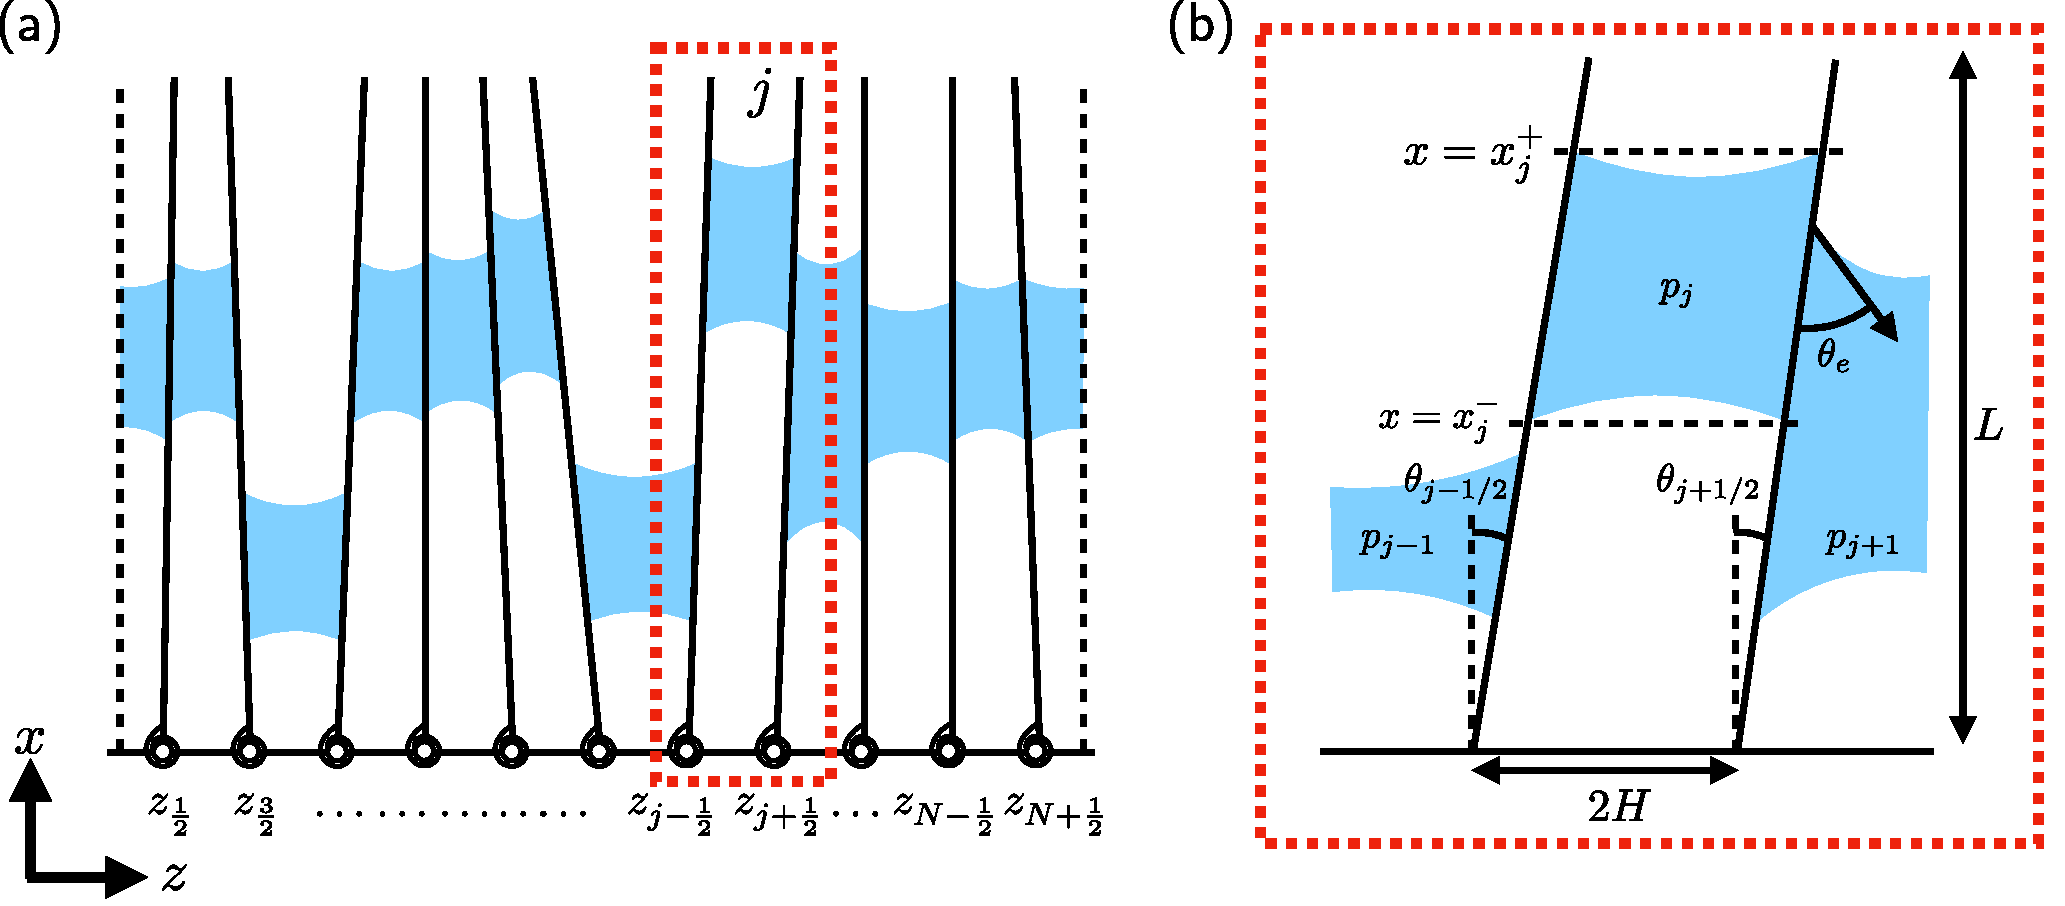
\includegraphics[width =0.95\textwidth]{SchematicMultiplePlates.pdf}
\caption{Modelling setup for interacting drop-channel systems. (a) Schematic diagram of the system of $N+1$ rigid plates, anchored at their base by torsion springs. (b) Detailed view of a single channel in the system. Note that the channel shape is described entriely by the adjacent deflection angles $\theta_{j-1/2}$ and $ \theta_{j+1/2}$.}\label{fig:Model:schematic}
\end{figure}

Each plate is anchored at a point along the $z$-axis, denoted $z = z_{j+1/2} = 2H(j+1/2),~j = 0,\dots, N$, by a torsion spring of stiffness $\kappa$ (this is consistent with channels of undeformed width $2H$ since the plates are assumed to be thin in comparison).  The torsion springs respond to applied torques by varying the angles (measured clockwise) they make with the $x$-axis; these are referred to as deflection angles, and are denoted by $\theta_{j+1/2}(t)$. The width of the $j^{\th}$ channel, at a perpendicular distance $x$ from its base is
\begin{equation}\label{E:Model:Modelling:ChannelWidth_withangles}
h_j(x,t) = 2H + x\tan\left( \theta_{j+1/2}\right) -x\tan \left(\theta_{j-1/2}\right),
\end{equation}
valid for $0 < x < L$. Note that the deflection angles scale with the channel aspect ratio $\alpha  = H/L \ll L $ so  changes in channel length in the $x$-direction because of plate tilting are negligible in comparison with $L$. This assumption also means that the channel widths can be approximated as
\begin{equation}\label{E:Model:Modelling:ChannelWidth}
h_j(x,t) = 2H + x \dthetaj(t)
\end{equation}
for $j = 1,\dots, N$, where $\dthetaj  = \theta_{j+1/2} - \theta_{j-1/2}$ denotes the tapering angle of the $j^{\text{th}}$ channel. Henceforth, the range of the index $j$ is suppressed -- it is always $j = 1,\dots, N$ -- and periodic conditions are assumed: any quantity with subscript $ 0$ or $N+1$ takes the same value as that quantity with subscript $N$ and $1$, respectively.

Droplets have (two-dimensional) volumes denoted by $V_j$ and make a liquid bridge between the channel walls. The $j^{\th}$ droplet wets the channel over the region $\xleftj(t)< x < \xrightj(t)$. (Note that whilst the channels are not necessarily symmetric about their midpoint -- $\theta_{j-1/2} \neq \theta_{j+1/2}$ in general -- it is consistent to assume that the meniscus positions are equal on each wall of the channel, as the deflection angles are small and the channel width thus varies slowly along its length.)

\subsection{Fluid Motion}
As before, lubrication theory is used to model the motion of the droplet. The pressure within the droplet in the $j^{\text{th}}$ gap, $p_j(x,t)$, satisfies Reynolds' equation~\citep{Leal2007}
\begin{equation}\label{E:Model:Modelling:ReynoldsEq}
 \ddp{h_j}{t}= x \ddp{\dthetaj}{t}= \ddp{}{x}\left[\frac{h_j^3}{12 \mu}\ddp{p_j}{x}\right] \quad \text{for} ~\xleftj(t)< x <\xrightj(t).
\end{equation}

For simplicity, we assume that condensation is negligible. As a result,  the flux of fluid through the menisci must balance that caused by the motion, giving the kinematic conditions
\begin{equation}\label{E:Model:Modelling:kinematic}
\dd{x^{\pm}_j}{t} = -\left.\frac{h_j(x_j^{\pm},t)^2}{12\mu}\ddp{p_{j}}{x}\right|_{x = x^{\pm}_j}.
\end{equation}

To solve~\eqref{E:Model:Modelling:ReynoldsEq} for the pressure within each drop, boundary conditions are required. There is a pressure jump across each meniscus caused by surface tension: as gravity is negligible, the menisci are arcs of circles whose curvature is $ 2\cos \theta_e/h_{j}(x_{\pm}^j,t)$ to leading order in $\alpha$ (the contribution to meniscus curvature from deflection angles comes in at $\mathcal{O}(\alpha)$). Taking the ambient pressure as reference, the liquid pressures at the menisci are therefore
\abeqn{E:Model:Modelling:laplace}{p_{j}(x^{+}_j, t) =- \frac{2\gamma \cos \theta_e}{2H + x_{+}^j \dthetaj},\qquad p_{j}(x^{-}_j, t) =- \frac{2\gamma \cos \theta_e}{2H + x_{-}^j \dthetaj}.}
Integrating equation~\eqref{E:Model:Modelling:ReynoldsEq} twice, using~\eqref{E:Model:Modelling:kinematic} and~\eqref{E:Model:Modelling:laplace} for the boundary terms, gives the $p_j$ in terms of $\dthetaj$, $\xbarj$, and their derivatives (see Appendix~\ref{Appendix:Reduction}).

\subsubsection{Pinned Drops}\label{S:Model:Model:Pinned}
During the motion, a droplet may reach the free end of the channel ($x = 1$) or the base ($x =0$). In practice, when it does so, the meniscus curvature relaxes by taking the value of the contact angle that ensures that the meniscus does not move (there is no flux of fluid there) until the contact angle has reached an advancing or receding angle (as discussed in detail for bendotaxis in a single flexible channel in Chapter 4). Here we have assumed, however, that the contact angle is fixed; we therefore encode pinned conditions by prescribing a no-flux condition instead of a Laplace pressure condition when the droplet is pinned. Explicitly, if the $j^\text{th}$ drop reaches the free end, we replace~\eqref{E:Model:Modelling:laplace}a with
\begin{equation}\label{E:Model:Modelling:kinematicPinned1}
\ddp{p_j}{x} = 0 \qquad \text{at}~x = x_j^+ = 1.
\end{equation}
so that by~\eqref{E:Model:Modelling:kinematic}, we have
\begin{equation}\label{E:Model:Modelling:kinematicPinned2}
\dd{\xrightj}{t} = 0,
\end{equation}
meaning that the meniscus does not subsequently move, and the droplet is said to be pinned. (Note that regardless of the droplet's pressure, it cannot be `unpinned', which may occur in practice as we saw in Chapter 4.)

Similarly, if the $j^\text{th}$ drop reaches the base, we replace \eqref{E:Model:Modelling:laplace}b by
\begin{equation}\label{E:Model:Modelling:kinematicPinned3}
\ddp{p_j}{x} = 0 \qquad \text{at}~x = x_j^- = 0,
\end{equation}
and hence $x_j^- = 0$ in the subsequent motion. We are, however, primarily interested in the behaviour before droplets are pinned, so consider boundary conditions~\eqref{E:Model:Modelling:kinematic}--\eqref{E:Model:Modelling:laplace} to be the default, which hold henceforth unless otherwise specified.

\subsection{Torque balance}
The pressure within each droplet has thus been determined (from~\eqref{E:Model:Modelling:ReynoldsEq}--\eqref{E:Model:Modelling:laplace}) in terms of the tapering angles, $\theta_{j+1/2}$,  the meniscus positions, $x_j^{\pm}$, and the time derivatives of both of these. To find a relationship between tapering and meniscus positions, a torque balance on each plate is considered.

Each plate is subject to torques from the liquid pressure within drops in the neighbouring channels, from interactions with neighbouring plates, and from the restoring spring torque. The fluid pressure torque on the $(j+1/2)^{\th}$ plate is
\begin{equation}\label{E:Model:Modelling:LaplaceTorque}
\tau_{\text{L}}^{j+1/2} = \int^{\xrightj}_{\xleftj} x p_{j}~\mathrm{d}x -  \int^{\xrightjj}_{\xleftjj} x p_{j+1}~\mathrm{d}x.
\end{equation}
\subsubsection{Plate contact}
For the case of flexible channel walls, considered in Chapter 2--4, there were two scenarios when the walls came into contact: regime II (making contact at a single point) and regime III (making contact along a portion of their length). However, for rigid plates, whose slopes are constant along their length, regime III has no analogue, so we model plate-plate interactions in a different way -- by including a van der Waals force between the plates. This force acts to repel beams strongly when they come close to touching (we also include a weak attraction to avoid bouncing out of contact). We assume that the van der Waals force is a point force on the end of the plates. The long range attraction and short range repulsion -- which prevents channel widths reaching zero -- is captured (see Figure~\ref{fig:Model:vanderWaals}) by taking the magnitude of the van der Waals forces between the $(j-1/2)^{\th}$ and $(j+1/2)^{\th}$ plates to be
\begin{equation}\label{E:Model:Modelling:vdwForce}
F_{j}(t) = A\left[\left(\frac{2H \varepsilon}{h_j(x = L,t)}\right)^9 - \left(\frac{2H\varepsilon }{h_j(x = L,t)}\right)^3\right],
\end{equation}
where $A$ is a constant force which sets the scale of plate-plate interaction forces and $\varepsilon$ is a small positive number (the equilibrium separation caused by van der Waals forces alone is $2H \varepsilon \ll 2H$).

\begin{figure}[t]
\centering
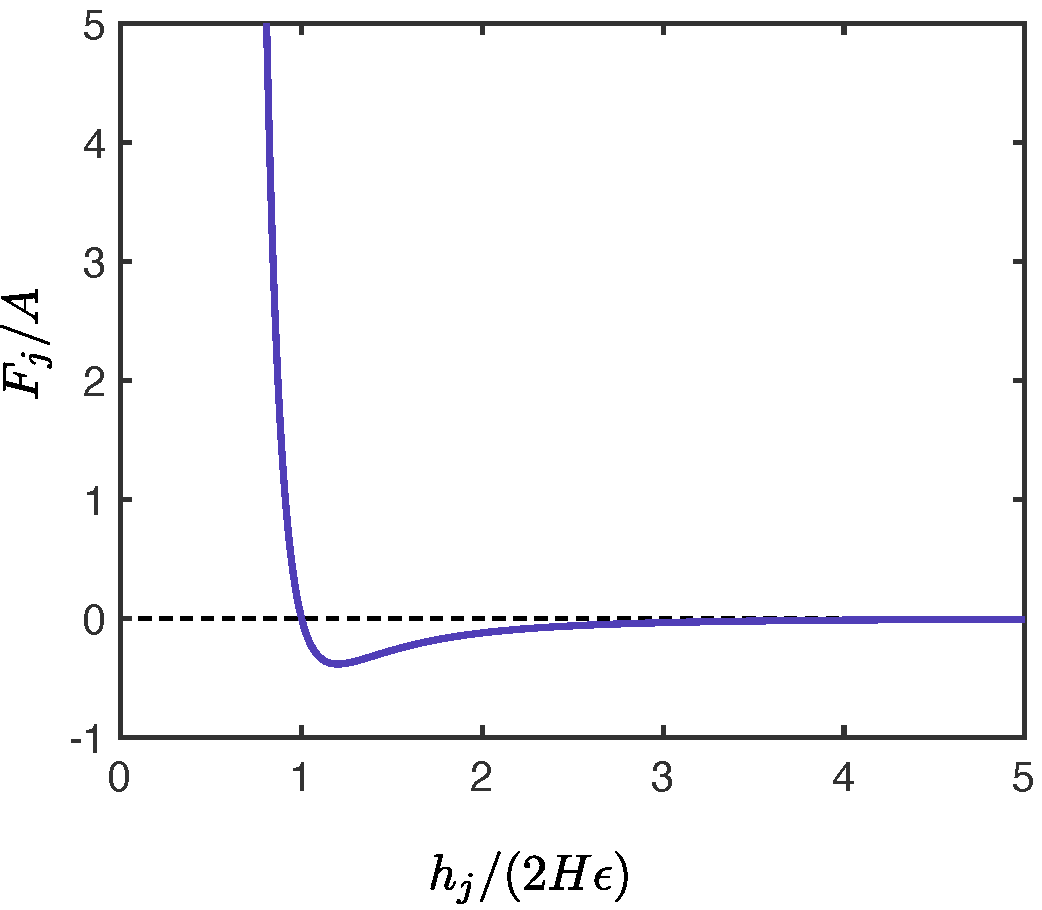
\includegraphics[scale=0.4]{vanderWaals}
\caption{Plot of the dimensionless function $F_j/A$ defined in equation~\eqref{E:Model:Modelling:vdwForce}. }\label{fig:Model:vanderWaals}
\end{figure}

The torque on the $(j+1/2)^{\th}$ plate due to van der Waals forces is then
\begin{equation}\label{E:Model:Modelling:vdwTorque}
 \tau^{\text{vdW}}_{j+1/2} = L\left[F_j(t) - F_{j+1}(t) \right].
\end{equation}

%Note that, provided it is weakly attractive at long range and strongly repulsive at short range, the particular expression for the van der Waals torque is unimportant and does not significantly alter the results of this chapter (appendix~\ref{Appendix:vanderWaals}).
\subsubsection{Torque balance equation}
The van der Waals and pressure-induced torques must be balanced by elasticity -- here represented by the restoring torque from the torsion spring. For a Hookean torsion spring, the restorative torque exerted on the $(j + 1/2)^\text{th}$ plate is
\begin{equation}\label{E:Model:Modelling:restorativeTorque}
\tau_{H}^{j+1/2} = \kappa \theta_{j+1/2}.
\end{equation}

A balance between damping within the spring and restorative torque, and van der Waals and fluid pressure torques gives
\begin{equation}\label{E:Model:Modelling:torqueBalance}
C_{\text{p}}\dd{\theta_{j+1/2}}{t} + \kappa \theta_{j+1/2}=\int^{\xrightj}_{\xleftj} x p_{j}~\mathrm{d}x -  \int^{\xrightjj}_{\xleftjj} x p_{j+1}~\mathrm{d}x + \tau^{\text{vdW}}_{j+1/2}
\end{equation}
where $C_{\text{p}}$ is the angular damping coefficient of the spring. Here  the particular form of the van der Waals torques has been  suppressed to reflect its unimportance (it is the characteristic short range repulsion and long range attraction, rather than the exact expression, of the van der Waals term that is important).

\subsection{Initial conditions}\label{S:Model:InitialConditions}
The system of differential equations is closed by specifying initial conditions
\begin{equation}\label{E:Model:Modelling:InitialConditions}
\xrightj(0) = x_{j,0}^{+}, \quad \xleftj(0) = x_{j,0}^{-}, \quad \theta_{j+1/2}(0) = \theta_{j+1/2}^0.
\end{equation}
These initial conditions implicitly specify the drop volumes, which must be conserved throughout the motion. Neglecting the missing volume contribution from the arc of the meniscus (which scales with the channel aspect ration $\alpha \ll 1$), conservation of volume can be expressed as $\mathrm{d}V_j/\mathrm{d}t = 0$, where
\begin{equation}\label{E:Model:Modelling:Volumes}
V_j = \left[\xrightj(t) - \xleftj(t)\right]\frac{h_j(\xrightj,t) + h_j(\xleftj,t)}{2}.
\end{equation}
(Note that $\mathrm{d}V_j/\mathrm{d}t = 0$ holds automatically when the kinematic conditions~\eqref{E:Model:Modelling:kinematic} hold).
\subsection{Non-dimensionalization}\label{S:Model:NonDim}
We non-dimensionalize the problem by choosing scales for spatial variables that are motivated by the channel geometry. The time scale emerges from of a balance between viscosity and capillarity, as before. In particular, we let
\begin{align}\label{E:Model:NonDim:Scales1}
\hat{t} &= \frac{H |\gamma \cos \theta_e|} {\mu L^2}t, &  (\hat{x},\hat{x}_j^{\pm})&= \frac{1}{L}(x,x_{j}^{\pm}), & \hat{h}_j &= \frac{1}{2H}h_j,
\end{align}
where dimensionless variables are denoted by $\hat{\cdot}$. In each of the models we have developed so far in this thesis, we have taken a  pressure scale that is set by a balance between beam bending and Laplace pressure. The equivalent scaling in this torsion spring model is that obtained by balancing the restorative spring torque and the fluid pressure torques in equation~\eqref{E:Model:Modelling:torqueBalance}; we therefore let
\begin{equation}\label{E:Model:NonDim:PressureScaling}
\hat{p}_j = \frac{L^3}{ 2H \kappa}p_j.
\end{equation}
Note that, in contrast to the flexible case, the behaviour of the whole, rather than half, of the channel is modelled -- this difference is responsible for the apparent extra factor of two. The torques generated by plate interactions are non-dimensionalized by scaling with the typical scale of the restoring torque scale, $2H\kappa/L$, i.e.
\begin{equation}\label{E:Model:NonDim:BeamInteractionTorqueScaling}
\hat{\tau}_{j+1/2}^{\text{vdW}} = \frac{L}{2H \kappa} \tau_{j+1/2}^{\text{vdW}}.
\end{equation}
Deflection angles are scaled by the aspect ratio, i.e. we let
\begin{equation}\label{E:Model:NonDim:AngleScaling}
\hat{\theta}_{j+1/2} = \frac{L}{2H}{\theta}_{j+1/2},
\end{equation}
and the dimensionless channel tapering is $\Delta \hat{\theta}_{j} = \hat{\theta}_{j+1/2} - \hat{\theta}_{j-1/2}$. The dimensionless channel widths are then
\begin{equation}\label{E:Model:NonDim:DimensionlessChannelWidth}
\hat{h}_j(x,t) = 1 + \hat{x}\Delta \hat{\theta}_{j}.
\end{equation}


\subsection{Statement of the problem}
In terms of these scaled variables, Reynolds' equation~\eqref{E:Model:Modelling:ReynoldsEq} reads
\begin{equation}\label{E:Model:NonDim:ReynoldsEq}
 \hat{x} \ddp{ \Delta \hat{\theta}_{j}}{\hat{t}}= \frac{1}{3|\Gamma|}\ddp{}{\hat{x}}\left[\hat{h}_j^3\ddp{\hat{p}_j}{\hat{x}}\right] \qquad \text{for} ~~\hat{x}_{-}^j(\hat{t})< \hat{x} <\hat{x}_{+}^j(\hat{t}).
\end{equation}
Here
\begin{equation}\label{E:Model:NonDim:GammaDefinition}
\Gamma = \frac{\gamma \cos \theta_e L^3}{2 \kappa H^2}
\end{equation}
is the dimensionless surface tension, which compares the typical torque from surface tension, $L^2\gamma/H$, with the typical restoring torque from the torsional spring $\kappa H/L$. The parameter $\Gamma$ is analogous to the bendability $\nu$ we have considered throughout this thesis. Different wettability conditions are captured by the sign of $\Gamma$: $\Gamma > 0$ corresponds to a droplet that wets the channel walls ($\theta_e < \pi/2$), and $\Gamma < 0$ to a droplet that does not ($\theta_e > \pi/2$).

Inserting~\eqref{E:Model:NonDim:Scales1}--\eqref{E:Model:NonDim:DimensionlessChannelWidth} in the kinematic conditions~\eqref{E:Model:Modelling:kinematic} and pressure boundary conditions~\eqref{E:Model:Modelling:laplace} gives
\begin{equation}\label{E:Model:NonDim:Kinematic}
\dd{\hat{x}_j^{\pm}}{\hat{t}} = -\frac{\hat{h}_j^2}{3|\Gamma|}\left.\ddp{\hat{p}_j}{\hat{x}}\right|_{\hat{x} = \hat{x}_{j}^{\pm}},
\end{equation}
and
\begin{equation}\label{E:Model:NonDim:Laplace}
\hat{p}_j(\hat{x}_{j}^{\pm}, \hat{t}) = -\frac{\Gamma}{1 + \hat{x}_j^{\pm}\Delta \hat{\theta}_j},
\end{equation}
respectively.

The torque balance becomes
\begin{equation}\label{E:Model:NonDim:TorqueBalance}
\hat{C}_p\dd{\hat{\theta}_{j+1/2}}{\hat{t}} + \hat{\theta}_{j+1/2} = \int_{x_{j}^{-}}^{x_{j}^{+}}\hat{x}\hat{p}_j ~\mathrm{d}x - \int_{x_{j+1}^{-}}^{x_{j+1}^{+}}\hat{x}\hat{p}_{j+1} ~\mathrm{d}x + \hat{\tau}_{j+1/2}^{\text{VDW}}
\end{equation}
where $\hat{C}_p= C_p H |\gamma \cos \theta_e|/(\mu \kappa L)$ is a dimensionless damping coefficient. We are primarily interested in the case where the dissipation occurs mainly due to the droplet viscosity, i.e. $\hat{C}_p \ll 1$; nevertheless, we retain the first term in~\eqref{E:Model:NonDim:TorqueBalance} due its importance in numerically solving the system (this is discussed further in \S\ref{S:Numerics}).  Note that this droplet-dominated dissipation is in contrast to previous torsion spring models of elastocapillary aggregation~\citep{Wei2014EPL, Wei2015PRSA} where configurations with wall-dominated damping, $\hat{C}_p\gg 1$, are considered. In~\eqref{E:Model:NonDim:TorqueBalance}, the dimensionless van der Waals torque is
\begin{equation}
\hat{\tau}_{j+1/2}^{\text{vdW}} = \hat{F}_{j} - \hat{F}_{j+1}
\end{equation}
where
\begin{equation}
\hat{F}_{j} = \frac{AL}{2H \kappa}\left[\left(\frac{\varepsilon}{\hat{h}_j(\hat{x} = 1, \hat{t})}\right)^9 -\left(\frac{\varepsilon}{\hat{h}_j(\hat{x} = 1, \hat{t})}\right)^3 \right]
\end{equation}
is the dimensionless van der Waals force between the $(j-1/2)^{\th}$ and $(j+1/2)^{\th}$ plates. The quantity $AL/(2H\kappa)$ compares a typical torque from the interaction between two plates separated by an $\mathcal{O}(\varepsilon)$ distance, with the typical restoring force from the torsion spring. To ensure van der Waals forces only become important for channels whose walls are very close to one another, we consider $AL/(2H\kappa) \ll 1$ here (we take $AL/(2H\kappa) = 10^{-6}$, $\varepsilon = 10^{-2}$ in all results presented in this chapter).

The dimensionless initial conditions,
\begin{equation}\label{E:Model:NonDim:InitialConditions}
\hat{x}_{j}^{\pm}(0) = \hat{x}_{j, 0}^{\pm}, \qquad \hat{\theta}_{j+1/2}(0) = \hat{\theta}_{j+1/2}^0,
\end{equation}
close the problem~\eqref{E:Model:NonDim:ReynoldsEq},~\eqref{E:Model:NonDim:TorqueBalance}--\eqref{E:Model:NonDim:Volume}, and also define the dimensionless droplet volumes
\begin{equation}\label{E:Model:NonDim:Volume}
\frac{V_j}{2HL} = \hat{V}_j = \left(\hat{x}_{j,0}^+ -\hat{x}_{j,0}^-\right))\frac{2 + \left(\hat{\theta}_{j+1}-\hat{\theta}_{j,0}\right) \left(\hat{x}_j^+ + \hat{x}_{j,0}^-\right)}{2},
\end{equation}
which represents the proportion of the channel a given drop would occupy if its walls were undeformed. Hats are henceforth dropped, and all quantities are dimensionless unless otherwise stated.

\subsection{System of differential equations}
It is convenient to work in terms of the mean meniscus position and drop half length, defined as
\begin{equation}\label{E:Model:DAEs:Definition_xbar_ell}
\xbarj = \frac{\xleftj + \xrightj}{2}\quad \text{and}\quad \ellj = \frac{\xrightj - \xleftj}{2}
\end{equation}
respectively. The meniscus positions are easily recovered from these as
\begin{equation}
\xrightj = \xbarj + \ellj, \quad \xleftj = \xbarj - \ellj.
\end{equation}
Equations~\eqref{E:Model:NonDim:ReynoldsEq}--\eqref{E:Model:NonDim:InitialConditions} can be reduced to a system of $2N$ ordinary differential equations (ODEs) for $\theta_{j+1/2}, \xbar_j$. Briefly (see Appendix~\ref{Appendix:Reduction} for further details), we first note that mass conservation requires
\begin{equation}\label{E:Model:DAEs:CoMass}
V_j = 2\ell_j(1 + \xbarj\dthetaj),
\end{equation}
to be constant throughout, which gives the droplet lengths $\ellj$ algebraically in terms of the $\xbar_j$ and $\Delta \theta_{j}$. We then integrate Reynolds' equation~\eqref{E:Model:NonDim:ReynoldsEq} twice alongside the Laplace pressure conditions~\eqref{E:Model:NonDim:Laplace} to obtain an expression for droplet pressures $p_j$ in terms of $\xbar_j, \Delta \theta_j$ and $\mathrm{d}(\Delta \theta_j)/\mathrm{d}t$. Inserting this expression into the torque balance equation~\eqref{E:Model:NonDim:TorqueBalance} gives the following $N$ ODEs:
\begin{multline}
-C_p\dd{\theta_{j+1/2}}{t} +|\Gamma|\left( \viscdamp_{j+1}\dd{\Delta \theta_{j+1}}{t} -  \viscdamp_{j}\dd{\Delta \theta_{j}}{t}\right) =\\
\theta_{j+1/2} - \tau^{\text{vdW}}_{j+1/2} + \frac{\Gamma}{2}\left[\frac{2\ell_{j}\Delta \theta_{j}I^2_j}{ h_j^+ h_j^-I^0_j} - \frac{2\ell_{j+1}\Delta \theta_{j+1}I^2_{j+1}}{ h_{j+1}^+ h_{j+1}^-I^0_{j+1}} -\right. \\
\left.\frac{(\bar{x}_{j+1}+\ell_{j+1})^2}{h_{j+1}^+} - \frac{(\bar{x}_{j+1}-\ell_{j+1})^2}{h_{j+1}^-} - \frac{(\bar{x}_{j}+\ell_{j})^2}{h_{j}^+} + \frac{(\bar{x}_{j}-\ell_{j})^2}{h_{j}^-}\right].\label{E:Model:DAEs:TorqueBal}
\end{multline}
Here the integrals $I_j^0, I_j^2,$ and $I_j^4$ are defined by
\begin{equation}\label{E:Model:DAEs:InDefinition}
I_j^n(t) = \int_{\xbar_j - \ell_j}^{\xbar_j + \ell_j} \frac{x^n}{(1 + x\dthetaj)^3}~\mathrm{d}x, ~n \in \mathbb{N}.
\end{equation}
The quantities
\begin{equation}\label{E:Model:DAEs:ViscDampDefn}
\viscdamp_j = \int_{\xbarj - \ellj}^{\xbarj + \ellj}\frac{x^2}{2}\ddp{p_j}{x}~\mathrm{d}x=  \frac{3}{4I^0_j}\left[I^0_j I^4_j - \left(I^2_j\right)^2\right].
\end{equation}
play the role of viscous dissipation in the droplet.

Inserting the expression for the pressure into the kinematic conditions~\eqref{E:Model:NonDim:Kinematic} (and taking their sum) gives $N$ ODEs:
\begin{multline}\label{E:Model:DAEs:Kinematic}
2\dd{\xbarj}{t}  +\frac{1}{2} \left[\frac{\ellj^2 + 2\ellj \xbarj}{h_j^+} + \frac{\ellj^2 - 2\ellj \xbarj}{h_j^-} -  \frac{I_2^j - \xbar_j^2 I_0^j}{I_0^j} \left(\frac{1}{h_j^+} + \frac{1}{h_j^-}\right)\right]\dd{(\dthetaj)}{t} =\\
-\frac{2\ellj\dthetaj\sgn(\Gamma)}{3I_0^j h_j^+ h_j^-} \left(\frac{1}{h_j^+} + \frac{1}{h_j^-}\right).
\end{multline}
The ODEs~\eqref{E:Model:DAEs:Kinematic} capture the balance between the two modes of droplet transport: squeezing (via the $\mathrm{d}(\dthetaj)/\mathrm{d}t$) and translating (via the $\mathrm{d}\xbarj/\mathrm{d}t$).

The differential equations~\eqref{E:Model:DAEs:TorqueBal} and~\eqref{E:Model:DAEs:Kinematic} are solved alongside the initial conditions
\begin{equation}\label{E:Model:DAEs:IC}
\theta_{j+1/2}(0) = \theta_{j+1/2}^0,\quad \xbar_j(0) =\xbar_j^0  = \frac{x_{j,0}^+ + x_{j,0}^-}{2},
\end{equation}
(Note that the procedure, and resulting differential equation system, is slightly different if droplets are pinned at the end of their channels -- see Appendix~\ref{Appendix:Reduction}.)


\section{The single channel case}\label{S:SingleChannel}
Having developed a model capable of describing bendotaxis in many interacting channels, we consider first the description of a droplet in a single channel. There are two reasons for studying this system: firstly it will allow us to verify that the equations derived in \S\ref{S:Model} (i.e. with torsion springs and rigid plates, rather than flexible plates as in Chapter 2--4) do indeed exhibit droplet transport to the free end of a single channel, regardless of wettability. The other reason is that by comparing the two models (flexible response and torsion spring response), information is gleaned about the relationship between the bending stiffness of beams in a flexible system, and the torsion stiffness included in the present system.  We would  like to keep our torsion spring model as faithful as possible to a model with flexible channel walls (which we expect to be more appropriate for describing a physical system). It might be expected that an appropriate choice of torsion stiffness would give quantitative agreement between the two models, giving greater confidence in the validity of results of this chapter when describing an array of flexible channels.

\subsection{Governing equations and numerical Solutions}
\begin{figure}[t]
\centering
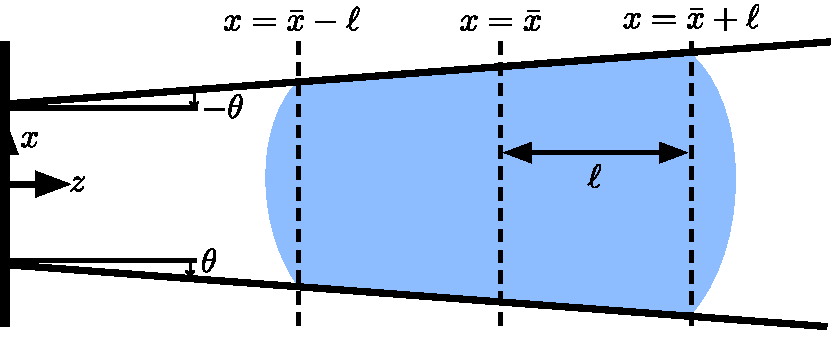
\includegraphics[scale=0.6]{SchematicSingleChannel_noghost.pdf}
\caption{Schematic diagram of a non-wetting droplet in a channel whose rigid walls are tethered at their base with torsion springs. Arrows indicate the clockwise direction in which angles are measured, i.e. $-\theta$ denotes an angle of magnitude $\theta$ measured anticlockwise about the $x$-axis.}\label{fig:SingleChannel:Schematic}
\end{figure}

A single drop-channel system is equivalent to the periodic system described in \S\ref{S:Model} with $N =2$ channels, one of which (say $j = 2$) contains a drop of trivial length (i.e. $\ell_2 = 0$). In this case, only one angle, $\theta_{3/2} = \theta$, needs to be considered; the other angles are $\theta_{1/2} = -\theta$ (by symmetry), and $\theta_{5/2} = -\theta$ (by periodicity), with the angle difference $\Delta \theta_{1} = 2\theta$ (see Figure~\ref{fig:SingleChannel:Schematic}). The system is described entirely by the angle $\theta$ and mean position $\xbar_1 = \xbar$ of the non-trivial drop. The droplet volume is $V\coloneqq V_1$ and is treated as a known parameter, and the droplet half length is $\ell = V/\left[2(1 + \xbar\Delta \theta)\right]$.

(Note that with this periodic formulation, it is possible that results for non-wetting drops with strong surface tension -- $\Gamma < 0$ with $|\Gamma| \gg 1$ -- may be unintentionally affected by van der Waals interactions between the beams which define the `ghost' channel containing no drop. This is resolved in what follows by including only van der Waals interactions between the beams surrounding the drop.



With these simplifications equations~\eqref{E:Model:DAEs:TorqueBal} and~\eqref{E:Model:DAEs:Kinematic} become (with suppressed indices):
\begin{align}
2\dd{\xbar}{t}+ \left[\frac{\ell^2 - 2\ell \xbar}{h^-} + \frac{\ell^2 + 2\ell \xbar}{h^+}-\frac{2(\xbar^2 I^0 - I^2)\bar{h}}{I^0 h^+ h^-}  \right]\dd{\theta}{t} +\frac{8\ell \theta\sgn (\Gamma)\bar{h}}{3I^0(h^+)^2 (h^+)^2} &= 0, \label{E:TwoPlates:DAEs1}\\
-2\left(C_p+|\Gamma|\viscdamp\right)\dd{\theta}{t}- \theta + \tau^{\text{vdW}} - \frac{\Gamma}{2}\left[\frac{4\ell \theta I^2}{I^0 h^+ h^-} + \frac{(\xbar + \ell)^2}{h^+} - \frac{(\xbar - \ell)^2}{h^-}\right]&=0\label{E:TwoPlates:DAEs2}
\end{align}
where $h^{\pm} = 1 + (\xbar \pm \ell)\Delta \theta, ~\bar{h} = 1 + \xbar\Delta \theta$ are the channel widths at the menisci and at the mean meniscus position, respectively. The system~\eqref{E:TwoPlates:DAEs1}--\eqref{E:TwoPlates:DAEs2} is closed by specifying initial conditions
\begin{equation}\label{E:TwoPlates:IC}
\xbar(0) = \xbar_0, \qquad \theta(0) = \theta_0.
\end{equation}

Figure~\ref{fig:TwoPlates:NumSols} shows traces of meniscus positions $x^{\pm} = \xbar \pm \ell$ and channel tapering $\Delta \theta$, obtained by solving equations~\eqref{E:TwoPlates:DAEs1}--\eqref{E:TwoPlates:DAEs2} numerically using the stiff ODE solver \textsc{ODE15s} implemented in \textsc{matlab}. As discussed in Chapter 2 for the flexible case, a stiff solver is required because of the different time scales present: as $\theta_0 = 0$, the beams offer no restoring force to balance the capillary pressure to begin with, so there is a short time scale on which damping from droplet viscosity must balance the capillary torque. During this short time scale, the droplet does not move very far -- it ultimately moves on a longer time scale during which the torsion spring resistance is important (these time scales are formally distinguishable in the case of weak surface tension, discussed later in this section). This early response can be seen in numerical solutions: see Figure~\ref{fig:TwoPlates:NumSols}, for example, in which the deflection angle in a numerical solution of~\eqref{E:TwoPlates:DAEs1}--\eqref{E:TwoPlates:DAEs2} with $\Gamma = 5$ reaches 90$\%$ of its final value in less than $1\%$ of the time taken for the droplet to reach the end of the channel. As we shall see, this separation of timescale is even more pronounced for $\Gamma = 0.1$ but is not resolved on the scale of Figure~\ref{fig:TwoPlates:NumSols}.

\begin{figure}[h!]
\centering
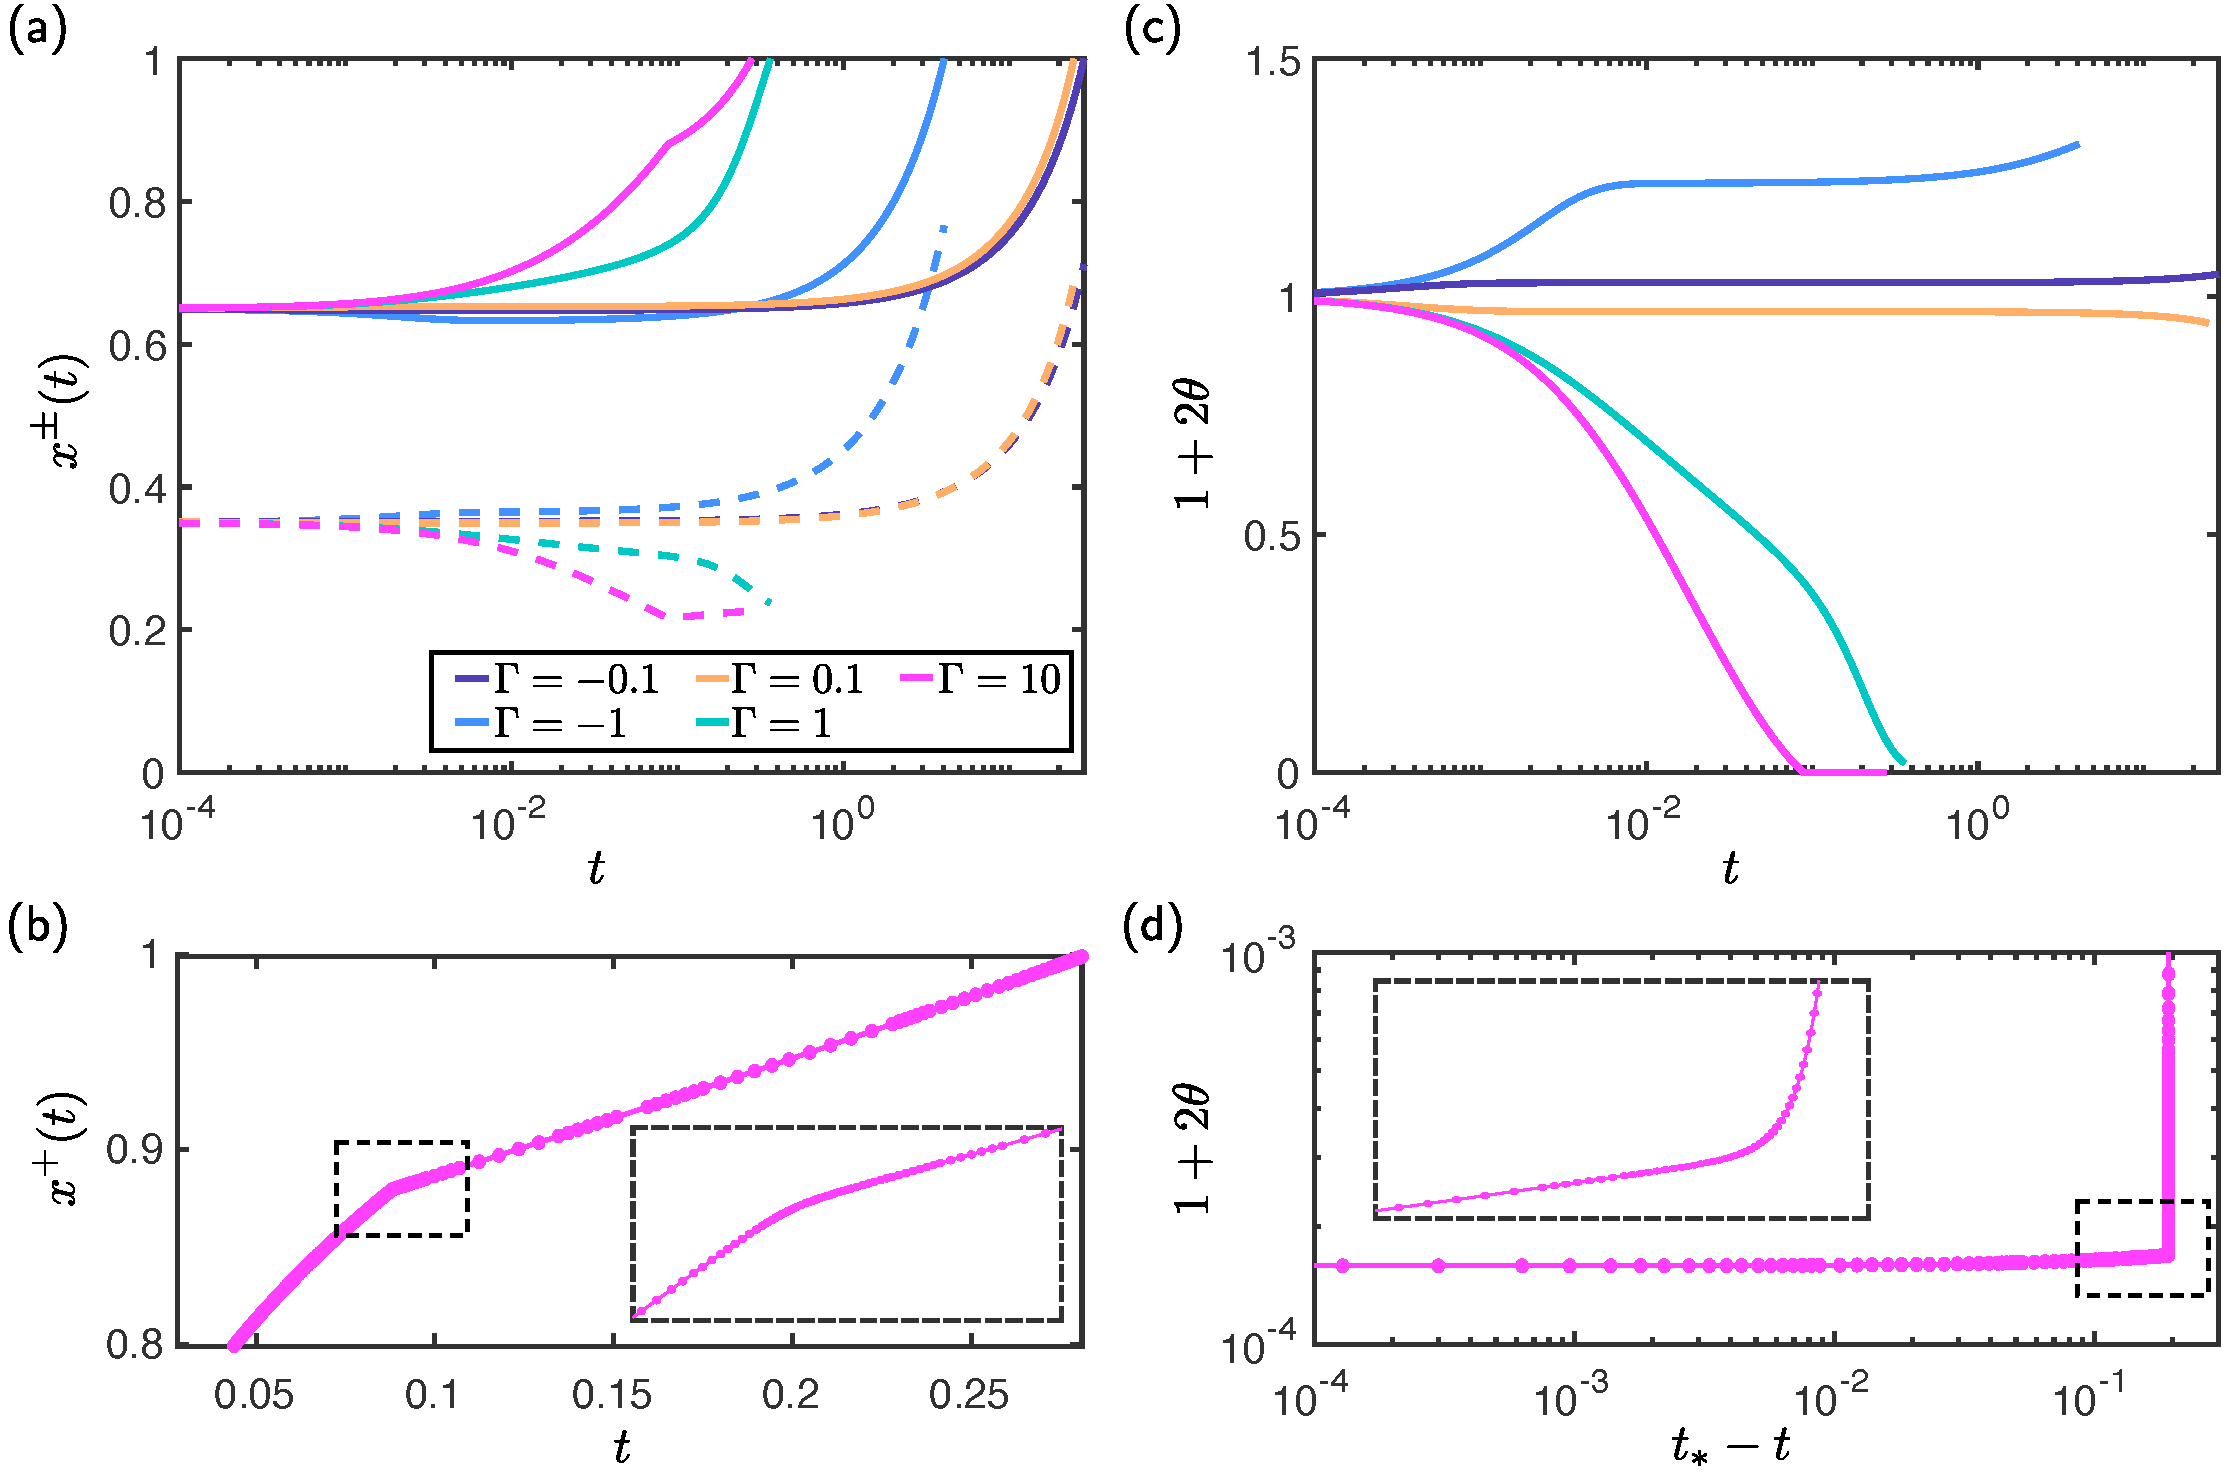
\includegraphics[width = 0.95\textwidth]{Traces_menisci_and_tapering.pdf}
\caption{Numerically-obtained solutions of equations~\eqref{E:TwoPlates:DAEs1}--\eqref{E:TwoPlates:DAEs2} with $\theta_0 = 0, \xbar_0 = 0.5$ and $V = 0.3$. (a): Traces of $x^{+} = \xbar+\ell$ (solid lines) and $x^{-} = \xbar-\ell$ (dashed lines) plotted on semi-logarithmic axes for four values of the dimensionless surface tension $\Gamma$ as indicated by the legend. The traces end when $x^+ = 1$, denoted $t =t_*$. (b): Portion of the  $\Gamma = 10$ trace indicated by the black dashed box in (a) (plotted on linear axes) showing constant velocity motion into the wedge. The rapid change in slope occurs when the plate ends are sufficiently close for van der Waals forces to be significant ($1 + 2\theta \approx 0$). Points indicate the mesh (in time) used in the numerical solution. The inset shows the behaviour close to the rapid change in speed, indicating that the traces shown in (a) and (b) are well resolved. (c): Traces of the channel width at the free end, $1 + 2 \theta$ on semi-logarithmic axes (colours are as in (a)). (d) Plot of channel width as a function of $t_* -t$ on logarithmic axes, corresponding to the region shown by the black dashed box in (c) with dots again indicating the mesh in time. Note that the channel does not close entirely, $1 + 2\theta >0$ (the distance at which van der Waals force is zero is taken to be $10^{-3}$). Inset: zoomed in on region indicated by the black box in (c), demonstrating that the channel width is also well resolved.}
\label{fig:TwoPlates:NumSols}
\end{figure}

These numerical solutions demonstrate that the model described in \S\ref{S:Model} describes droplet transport by bendotaxis in a single channel that is wettability independent (in this case, the `bending' occurs in the torsion spring, rather than in the channel walls): droplets are transported to the free end (the trajectories $x^{+}(t)$ shown in Figure~\ref{fig:TwoPlates:NumSols}(a) reach $x = 1$) regardless of whether the droplets wet the channel ($\Gamma > 0$) or not ($\Gamma < 0$), a result that is generic in numerical solutions of~\eqref{E:TwoPlates:DAEs1}--\eqref{E:TwoPlates:DAEs2} (provided droplets do not start too close to the base and make contact during the early time scale, where menisci move in opposite directions). This droplet motion is accompanied by an inwards deflection when the droplets wets the channel ($\Delta \theta = 2\theta <0$ in Figure~\ref{fig:TwoPlates:NumSols}(b)) and outwards when it does not ($\Delta \theta = 2\theta >0$), as we also saw in the flexible case. There are further similarities: droplets accelerate along the channel, and beam-beam interactions play a role when surface tension is sufficiently strong: the magenta traces ($\Gamma = 10$) in Figure~\ref{fig:TwoPlates:NumSols} show that the `+' meniscus decelerates briefly at $t\approx 10^{-1}$, when the channel walls come sufficiently close for van der Waals force to be important. The short range repulsion associated with this force means the channel does not close entirely (Figure~\ref{fig:TwoPlates:NumSols}(d)) but forms a triangle-like wedge (albeit with a narrow gap). This is in contrast to the flexible case considered in Chapters 2--4, where the beams make contact. It might be expected that the lubrication approximation breaks down as the droplet moves into this wedge, but we note that the constant speed of imbibition into it (Figure~\ref{fig:TwoPlates:NumSols}(b)) is consistent with theory and experiment describing the similar scenario of droplet imbibition into rigid wedges~\citep{Reyssat2014JFM}.




\subsection{Comparison between torsion spring and flexible cases}\label{S:SingleChannel:FlexibleComparison}
As discussed, we would like our torsion spring model, in which the spring stiffness $\kappa$ is known, to be as faithful as possible to a flexible model whose walls have a bending stiffness $B$. However, we would prefer to use the torsion spring model for multibody bendotaxis due to its relative simplicity. We therefore want to find an effective spring stiffness -- the value of $\kappa$ that gives quantitative agreement with the flexible case for a given value of $B$.

Note that $\kappa$ has the units of a force, while $B$ has the units of a force per unit length, so they must be related via a length scale. The present problem has two geometric length scales, $L$ and $H$ as well as the length scales defined by the position of the drop, say $X_d$, and the length of the drop (denoted $\Delta X$ in Chapters 2--4). It is not immediately obvious which is the correct choice. Here, we compare the results of a single channel to those of the flexible model described in Chapter 2 in the case of weak surface tension, $|\Gamma| \ll 1$, where analytic results can be found in both the flexible and torsion spring cases. In doing so, we identify the correct length scale and offer a suggestion on how to choose an effective spring stiffness.

The asymptotic analysis of equations~\eqref{E:TwoPlates:DAEs1}--\eqref{E:TwoPlates:DAEs2} in the limit $|\Gamma |\ll 1$ (see Appendix~\ref{Appendix:SmallGammaAnalysis} for full details) begins by assuming small deformations $|\theta| \ll 1$ for all $t>0$. The dynamics then decouple into two distinct time scales: on a fast ($\mathcal{O}(\Gamma)$) timescale, the drop does not make a net movement along the channel ($\xbar$ is constant), but the deflection angles respond to applied torques. At early times, this response arises from a torque imbalance: no resistive torque is offered by the torsion springs since $\theta_0 = 0$, but there is a non-trivial capillary pressure which must therefore be balanced by dissipation in the drop and plate. The angle evolution is given by
\begin{equation}\label{E:SingleChannel:SmallGamma:FastTimescaleEq}
\theta = -\Gamma V \xbar_0\left[1 - \exp\left(\frac{-1}{C_p + C_{d}^0}\frac{t}{|\Gamma|}\right)\right],
\end{equation}
where
\begin{equation}\label{E:SingleChannel:SmallGamma:SlowTimescaleEq}
C_{d}^0 = V^3\left(\frac{V^2}{240} + \frac{\xbar_0^2}{4}\right)
\end{equation}
is the leading-order term in the expansion of droplet dissipation for $|\Delta \theta| \ll 1$. The droplet itself moves on a long ($\mathcal{O}(1/|\Gamma|)$) timescale, with the mean meniscus position evolving according to the ODE
\begin{equation}\label{E:SingleChannel:SmallGamma:xbarODE}
\dd{\xbar}{t} = \frac{2|\Gamma|V}{3}\xbar.
\end{equation}
As discussed in Chapter 2, when the channel walls are flexible, and wall deflections are small, the droplet moves according to the ODE
\begin{equation}\label{E:SingleChannel:SmallGamma:xbarODE_flexible}
\dd{\xbar}{t} = \frac{|\nu| V}{6}\left(\xbar + \frac{V}{2}\right)^2.
\end{equation}
where $\nu = \gamma \cos \theta_e L^4/(BH^2)$.

Comparison of~\eqref{E:SingleChannel:SmallGamma:xbarODE} and~\eqref{E:SingleChannel:SmallGamma:xbarODE_flexible} suggests that the length scale relating $\kappa$ and $B$ is $X_d$, i.e. $\kappa \sim B/X_d$. This is perhaps unsurprising: in the flexible case, the further away from the clamped end that a (fixed) force is applied, the larger the deformation (note that this is necessary for bendotaxis to occur). Or, equivalently, two channels, whose flexible walls have different bending stiffnesses, may experience the same deformation from a droplet if it is father from the clamped end in the channel whose walls have a higher bending stiffness.

It is therefore not possible to find an `effective bending stiffness' which gives completely equivalent dynamic behaviour. However, we can find quantitative agreement between the flexible and torsion spring cases with respect to certain metrics (in the small $\Gamma$ limit). Here we consider one example: the time taken for the droplet to traverse a section of the between $x = f < 1$ and $x = 1$. This is the metric we used in our experimental study of bendotaxis in Chapter 3 as a proxy for the dynamic behaviour.

By solving the ODE~\eqref{E:SingleChannel:SmallGamma:xbarODE}, we find that the dimensionless bendotaxis time for a single torsion spring channel is
\begin{equation}\label{E:SingleChannel:SmallGamma:tX}
t_{f} = \frac{3}{2|\Gamma|V}\log\left(\frac{2-V}{2X-V}\right).
\end{equation}
In Chapter 2, we found the equivalent result for the flexible case:
\begin{equation}
t_{f}^{\text{flexible}} = \frac{6}{|\nu|V}\frac{1-f}{f}.
\end{equation}
Therefore quantitative agreement between the flexible and torsion spring cases (with respect to the bendotaxis time) can be had by considering a system whose spring stiffness is
\begin{equation}\label{E:SingleChannel:SmallGamma:EffectiveBending}
\kappa = \frac{2(1-f)}{f \log\left(\frac{2-V}{2f-V}\right)}\frac{B}{L}.
\end{equation}
In other words, the asymptotic results presented in Chapter 2 for a flexible channel of bending stiffness $B$ are identical to those for a torsion spring channel whose spring stiffness is chosen according to~\eqref{E:SingleChannel:SmallGamma:EffectiveBending}.



\section{Numerical solutions}\label{S:Numerics}
In this section, we present numerical solutions of the governing equations derived in \S\ref{S:Model}, and describe the numerical methods used to obtain them. Note that in the following sections (\S\ref{S:Numerics}--\S\ref{S:Discussion}), we consider only wetting drops ($\Gamma >0$); the corresponding results of these sections in the non-wetting case are discussed in \S\ref{S:NonWetting}.

\subsection{Details of numerical methods}\label{S:Numerics:Details}
To numerically solve the problem, we first express equations~\eqref{E:Model:DAEs:TorqueBal} and~\eqref{E:Model:DAEs:Kinematic} as a single matrix differential equation
\begin{equation}\label{E:NumSols:MDE:MatrixDifferentialEquation}
\underline{M}\dd{\underline{u}}{t} =\underline{f}.
\end{equation}
where $\underline{u} = (\theta_{3/2},\dots, \theta_{N+1/2},\xbar_1,\dots,\xbar_N)^\intercal$. Here $\underline{M}$ and $\underline{f}$ play the roles of a mass matrix and a force, respectively (note that $\underline{M}$ changes dynamically and captures pinning conditions, see Appendix~\ref{Appendix:MatrixDifferentialEquation} for more details, including explicit expressions for  $\underline{M}$ and $\underline{f}$). In this setting, the initial condition is
\begin{equation}\label{E:NumSols:MDE:IC}
\underline{u}^0 =\left(\theta_{3/2}^0, \dots, \theta_{N+1/2}^0,\xbar_1^0, \dots,\xbar_N^0\right)^\intercal.
\end{equation}

The matrix equation~\eqref{E:NumSols:MDE:MatrixDifferentialEquation} is  well-defined only if $\underline{M}$ has full rank. This is not the case when plate damping is neglected ($C_p = 0$); in this case, the first $N+1$ rows of $\underline{M}$ have zero row-sum, and hence $\underline{M}$ has a zero eigenvector $\underline{v}_0 =(1,\dots,1,0,\dots,0)^\intercal$. This elucidates the importance of retaining plate damping in the model.

Let us briefly consider $\underline{v}_0$: this eigenvector corresponds to increasing each of the deflection angles by an equal amount, without changing the positions or shapes -- and therefore capillary torques -- of the droplets. Increasing the deflection angles, however, increases the restoring torques from the torsion springs, resulting in a torque imbalance; when $C_p \neq 0$, this imbalance is resolved on a fast timescale where plate damping balances with restoring torque.

We therefore consider $0 < C_p \ll 1$  in the rest of this chapter (recall that the latter inequality ensures droplet damping dominates over plate damping). All results presented use $C_p= 10^{-3}$, but we have observed that numerical solutions display indistinguishable behaviour with $C_p = 10^{-5}, 10^{-4}$, and $10^{-3}$.

The problem~\eqref{E:NumSols:MDE:MatrixDifferentialEquation}--\eqref{E:NumSols:MDE:IC} is solved numerically using the \texttt{ODE15s} routine in \textsc{matlab}. At each time-step, the sparse mass matrix $\underline{M}$ is evaluated, with particular care taken in the computation of the integrals $I_j^n, n = 0,2,4$. Analytic expressions for the $I_j^n$ can be found for $|\dthetaj|>0$ by integrating~\eqref{E:Model:DAEs:InDefinition} by parts, and trivially for $\dthetaj=0$. This result is singular in the limit $|\dthetaj| \to 0$, so the $I_j^n$ are evaluated for $|\dthetaj|\ll 1$ by expanding the integrand in $|\dthetaj|$ and integrating term-by-term. (We are careful to ensure that the magnitude of errors introduced by truncating this sum fall below errors from numerical integration.)

\subsection{Numerical experiments}\label{S:Numerics:NumericalExperiments}
\begin{figure}[h!]
\centering
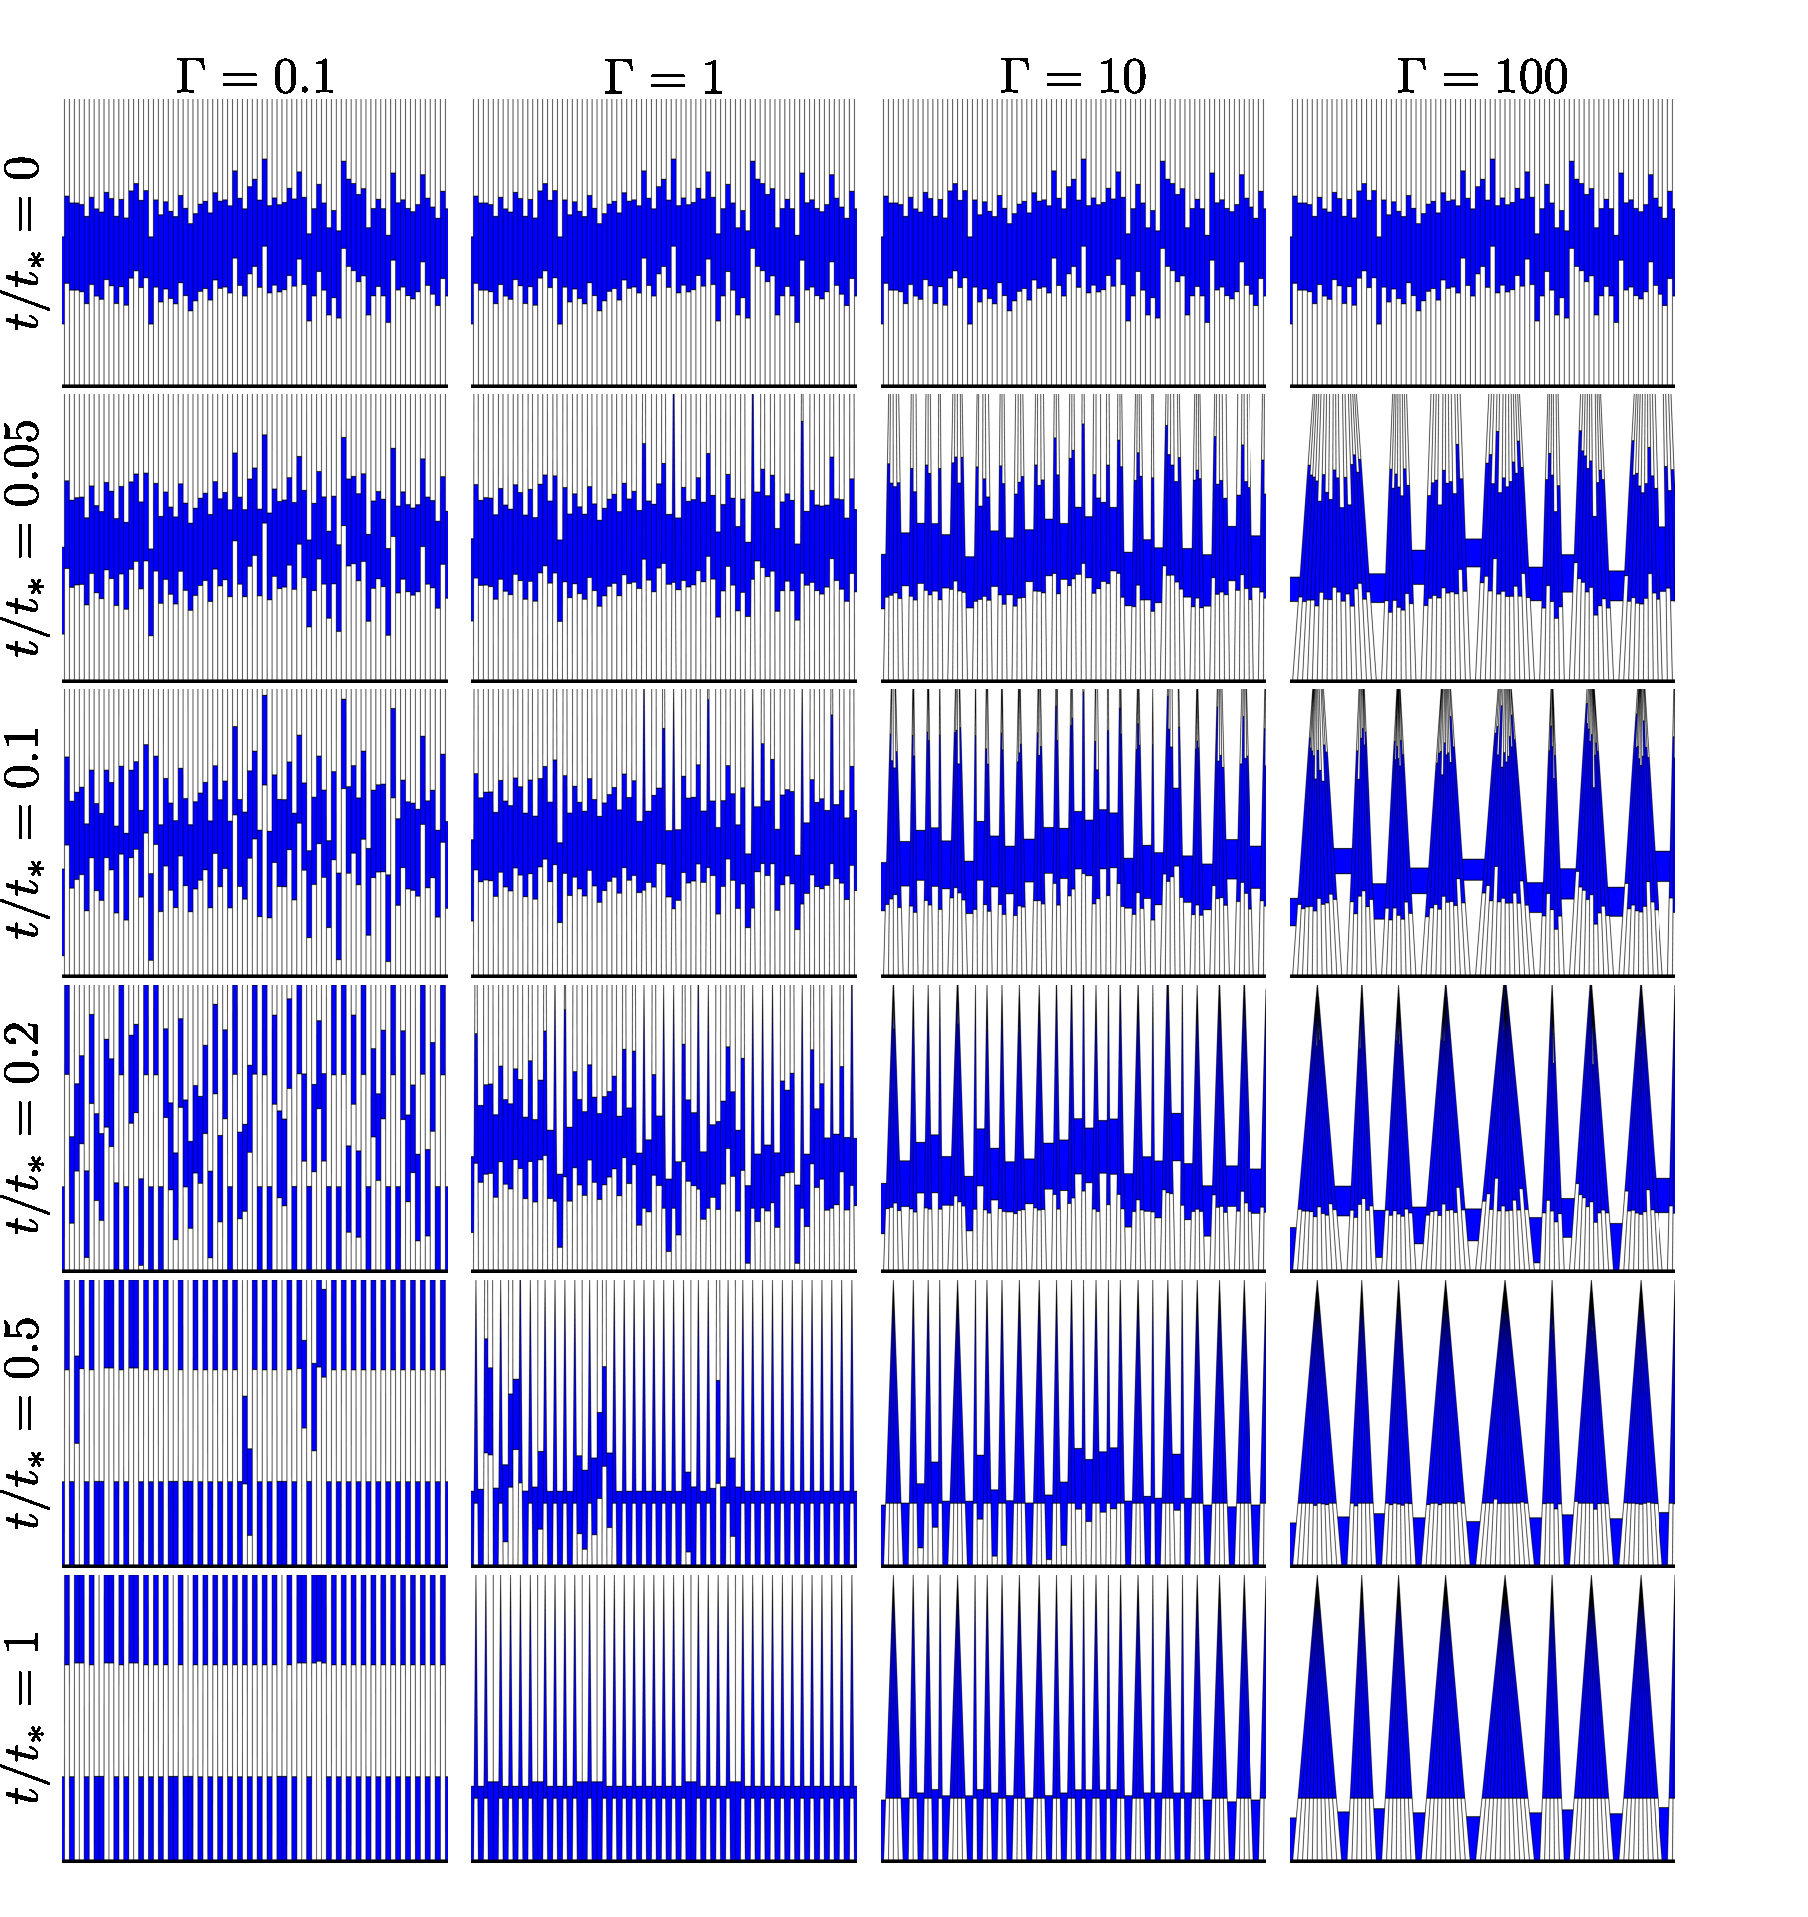
\includegraphics[width = \textwidth]{Snapshots.pdf}
\caption{Snapshots of arrays corresponding to numerical solutions of~\eqref{E:NumSols:MDE:MatrixDifferentialEquation} with random initial conditions~\eqref{E:Numerics:NumericalExperiments:RandomIC} (the initial conditions are the same for each value of $\Gamma$ with $\epsilon = 0.1$ and $\xbar_0 = 0.5$) and uniform volumes $V_j = 0.3$. The time at which the snapshot is taken is measured relative to $t_*$ -- the time at which every droplet has reached either end of the channel containing it. Here, $t_* \approx 300,~6,~1,~0.6$, for $\Gamma = 0.1,~1,~10,~100$ respectively. Note that the equations were solved for $N=199$ channels (i.e. $200$ plates), but only those with indices $1 < j < 80$ are shown here for clarity.}\label{fig:Numerics:Snapshots}
\end{figure}

\begin{figure}[t]
\centering
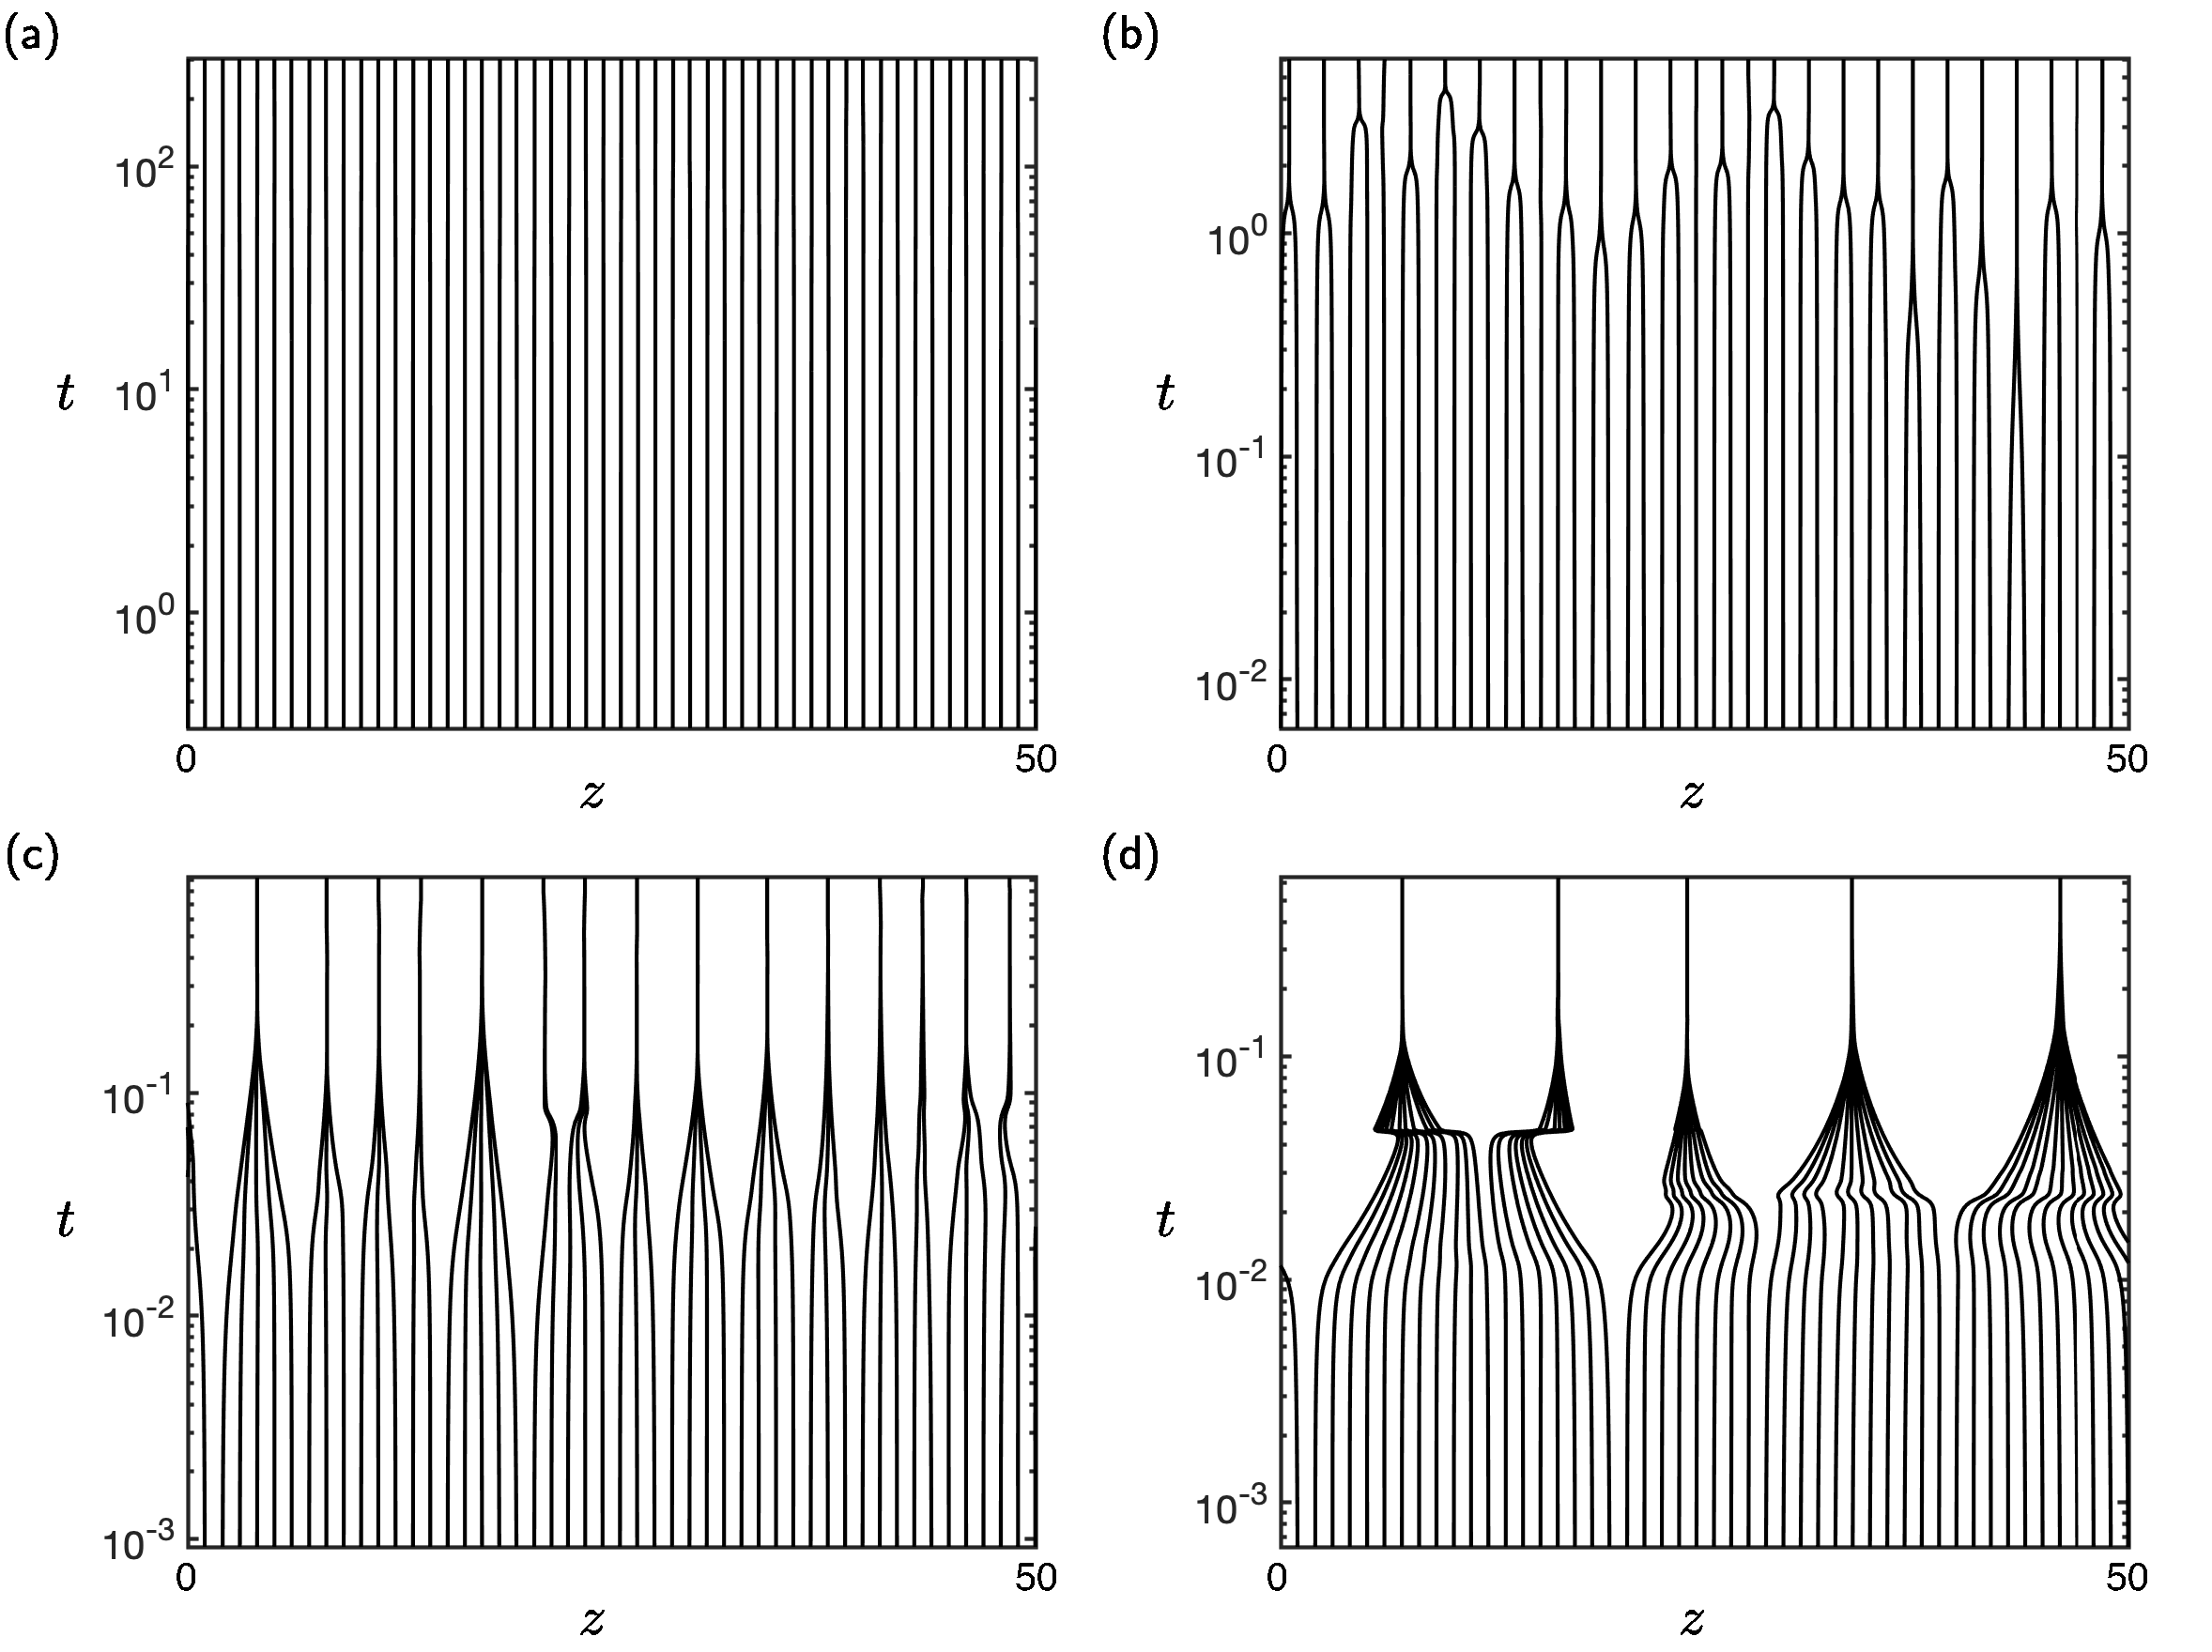
\includegraphics[width = \textwidth]{Spatiotemporal_combined.pdf}
\caption{Spatiotemporal plots of numerical solutions to~\eqref{E:NumSols:MDE:MatrixDifferentialEquation} with random initial conditions~\eqref{E:Numerics:NumericalExperiments:RandomIC} (with $\epsilon = 10^{-1}, \xbar_0 = 0.5$). Each subplot corresponds to a column of the snapshots displayed in Figure~\ref{fig:Numerics:Snapshots}, i.e. each  corresponds to a different value of $\Gamma$ as follows: (a) $\Gamma = 0.1$, (b) $\Gamma = 1$, (c) $\Gamma = 10$, (d) $\Gamma = 100$. Here $V_j = 0.3$, and $N=199$ channels consisting of $200$ plates (only 50 plates are shown for clarity).  Note that each curve in $(z,t)$ space corresponds to the trajectory of the end ($x=1$) of a single beam. The apparent kinks in (d) are the separation of large clusters into two smaller clusters (see main text).}\label{fig:Numerics:Spatiotemporal}
\end{figure}

\begin{figure}[t]
\centering
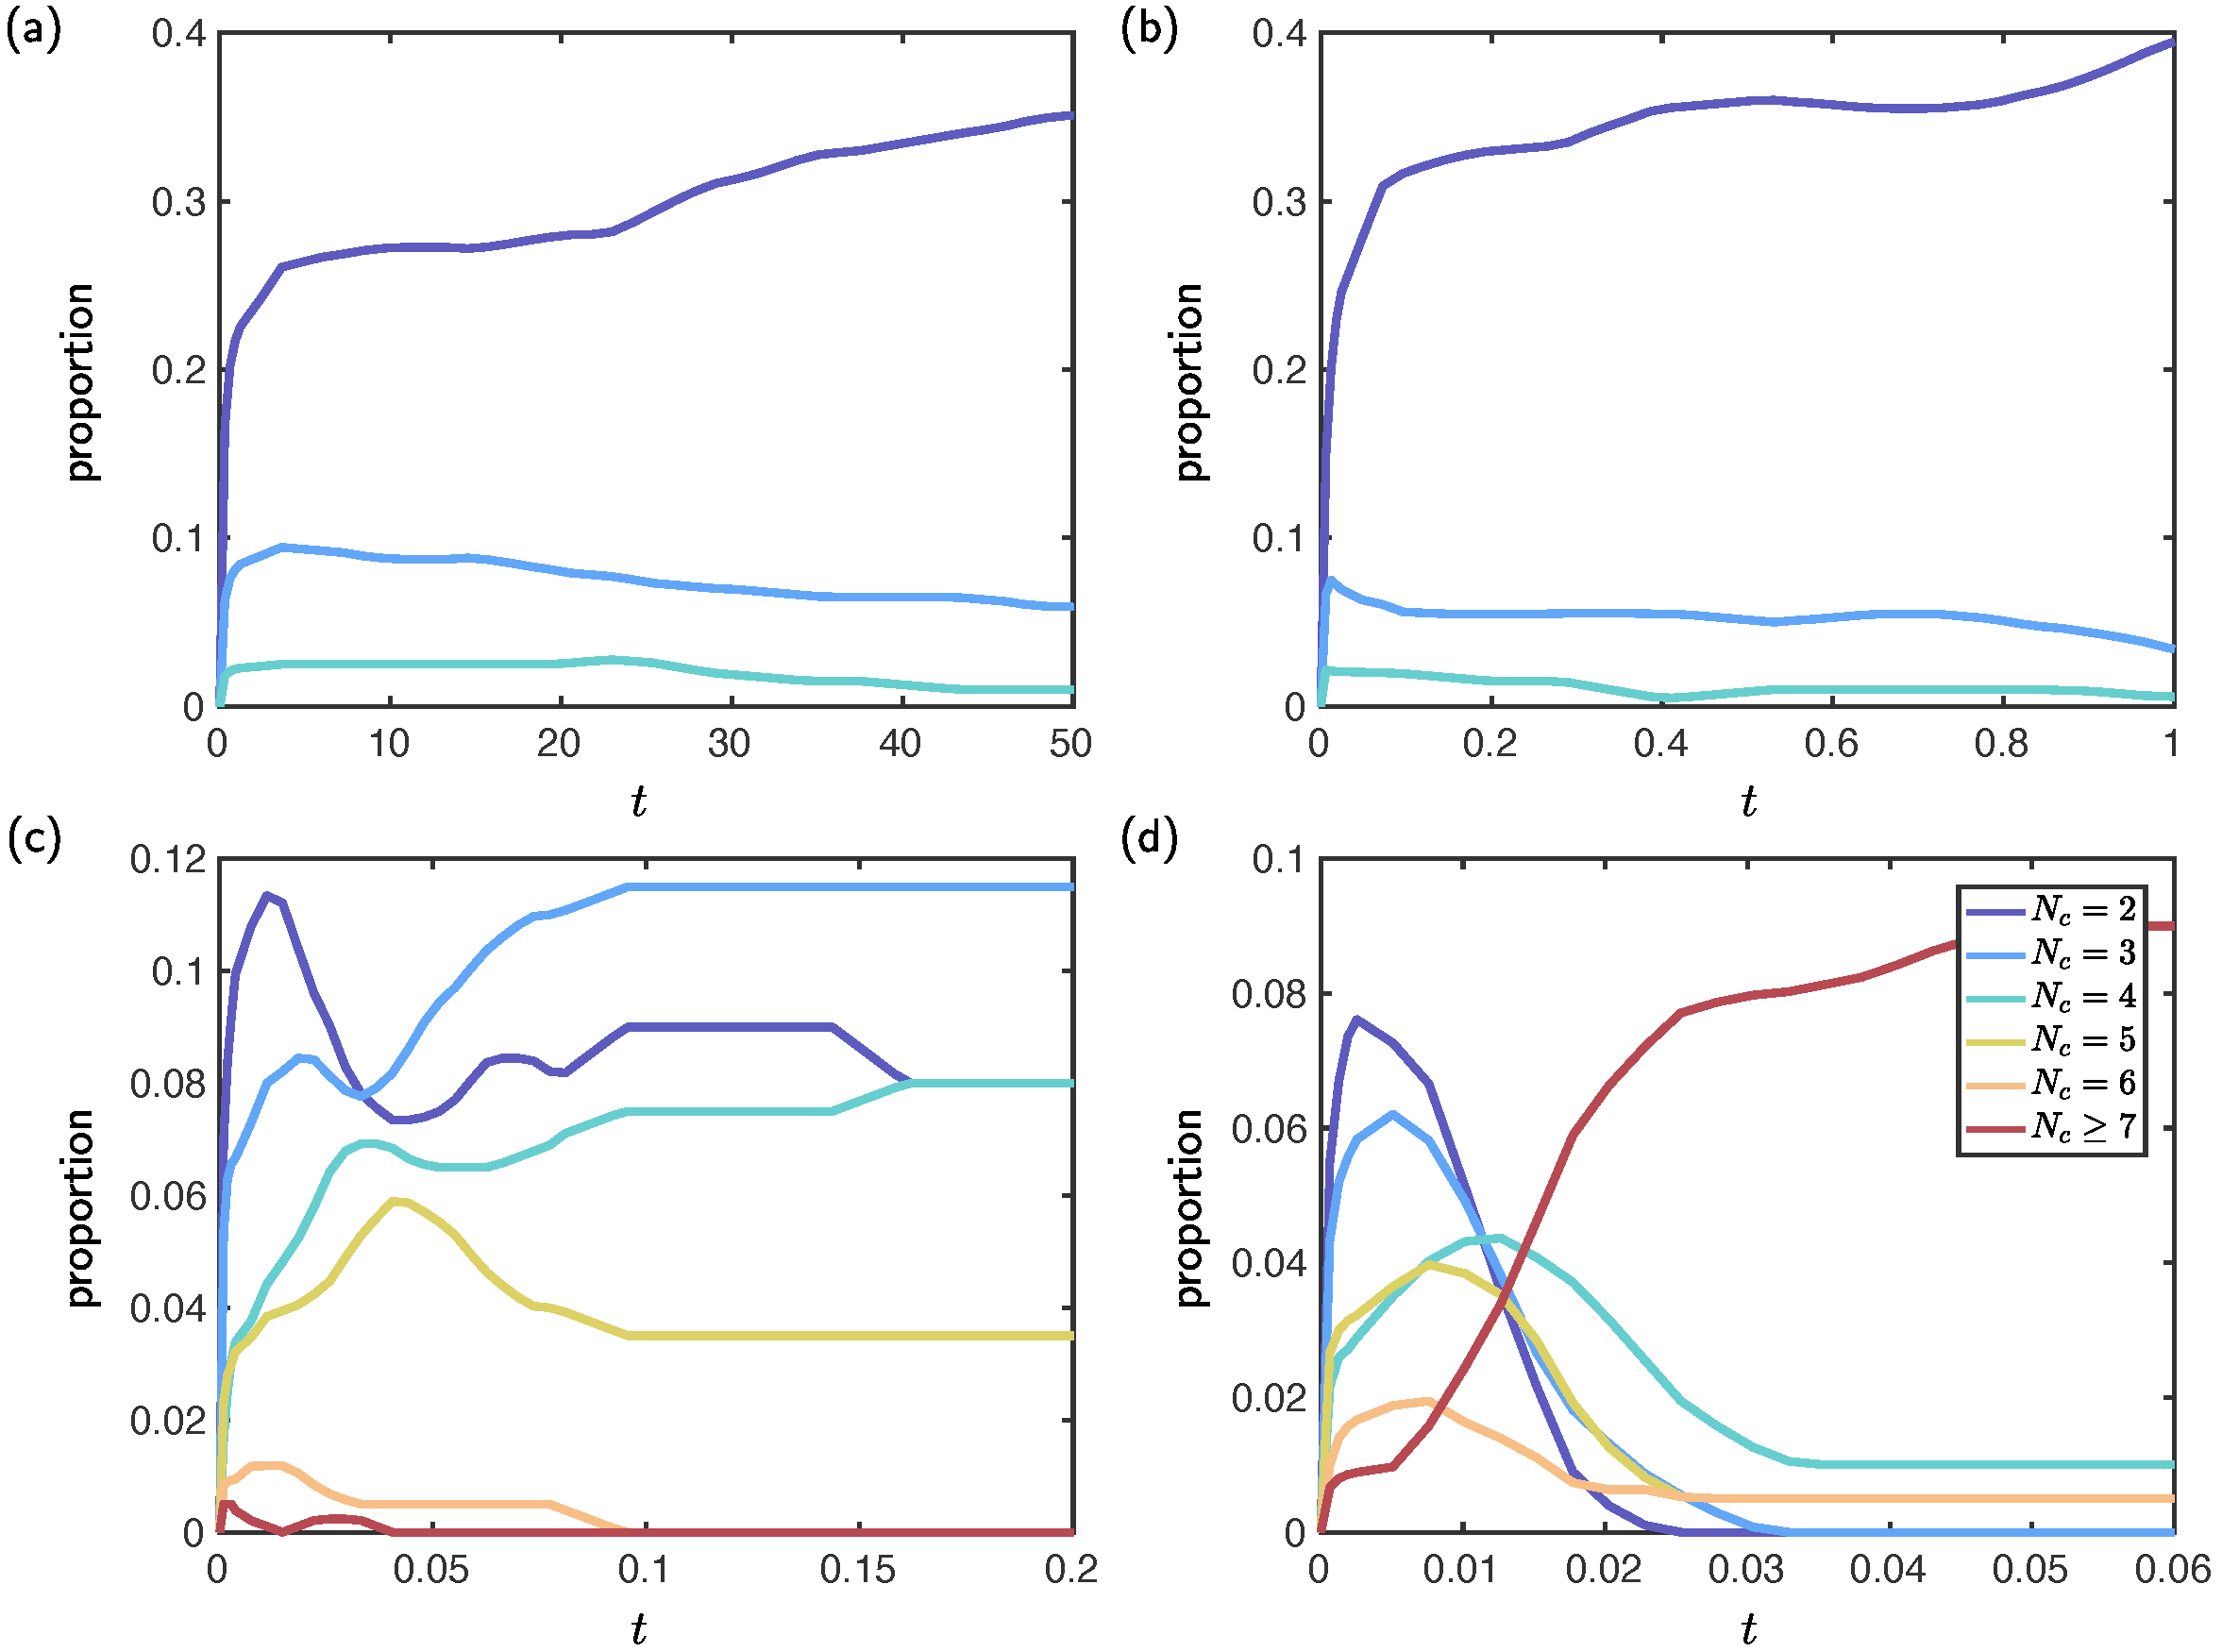
\includegraphics[width = 0.95\textwidth]{ClusterSizes}
\caption{Evolution of the proportion of clusters of each particular size $N_p$ (indicated in the legend in (d)) in numerical solutions~\eqref{E:NumSols:MDE:MatrixDifferentialEquation} with random initial conditions~\eqref{E:Numerics:NumericalExperiments:RandomIC}. Each subplot corresponds to a column of the snapshots, which are displayed in Figure~\ref{fig:Numerics:Snapshots}, i.e. each subplot corresponds to a different value of $\Gamma$ as follows: (a) $\Gamma = 0.1$, (b) $\Gamma = 1$, (c) $\Gamma = 10$, (d) $\Gamma = 100$. Here $V_j = 0.3$, and $N=199$ channels ($200$ plates). Note that the time axis only covers part of the motion (the curves are approximately time independent for times later than those shown).}
\label{fig:Numerics:ClusterSizes}
\end{figure}


Figure~\ref{fig:Numerics:Snapshots} displays the snapshots of the evolution of the droplet-channel array at various time-points measured relative to $t^*$ -- the time at which every drop is pinned at one, or both, of the ends of the channel. The snapshots show solutions for $\Gamma = 0.1, 1, 10$, and $100$; $\Gamma = 0.1$ corresponds to weak surface tension, whilst $\Gamma = 100$ corresponds to strong surface tension. The channel shapes, $h_j(x,t) = 1 + x\dthetaj$, and drop positions, $\xbar_j$, are obtained numerically (as described in the previous section) by solving~\eqref{E:NumSols:MDE:MatrixDifferentialEquation} with a random initial condition:
\begin{equation}\label{E:Numerics:NumericalExperiments:RandomIC}
\theta_{j+1/2} = 0, \quad \xbar_j = \xbar_0 + \epsilon \mathcal{R}_j.
\end{equation}
Here $\mathcal{R}_j$ is a (seeded) random number sampled from a normal distribution with zero mean and unity variance, and $\epsilon$ is a small, positive constant (note that the solutions shown in Figure~\ref{fig:Numerics:Snapshots} have the same initial condition).

Figure~\ref{fig:Numerics:Spatiotemporal} displays the corresponding spatiotemporal plots of the free end channel widths, $h_j(x=1,t) = 1 + \dthetaj$. Note that in each numerical experiment the same channel volumes $V_j$ are used as we are primarily interested in the influence of surface tension (via $\Gamma$). To quantify the aggregation process we define clusters: a channel is part of a cluster if it tapers inwards along its length ($\dthetaj < 0$), and channels with outwards tapering ($\dthetaj > 0$) are the boundaries of clusters. The size of a cluster, $N_p$, is defined to be the number of plates in the cluster (for example a cluster of size four consists of four plates which define three channels).

When surface tension is weak (left column in Figure~\ref{fig:Numerics:Snapshots} and~\ref{fig:Numerics:Spatiotemporal}(a)), the channels are deformed only slightly (not resolved on the scale of these plots) and a pairwise separation dominates. The vast majority of channels in this system form clusters of  two plates (see Figure~\ref{fig:Numerics:ClusterSizes}). Neighbouring drops move very slowly to opposite ends of the array, and approximately half of the droplets end up at the free end of channels. Here we see that the interactions between neighbouring channels prevents droplets transport to the free end, in some of the channels.

For stronger surface tension, deviations from the pairwise mode are observed. In particular, channels cluster into groups of different sizes that are not restricted to the set $2^{\mathbb{N}}$ (as was suggested in several similar studies of elasto-capillary aggregation, see \S\ref{S:Intro}). Figure~\ref{fig:Numerics:ClusterSizes} shows that a range of cluster sizes appear even at early times, although the largest clusters don't appear until later on. We also see that clusters can split: what appear to be discontinuities in Figure~\ref{fig:Numerics:Spatiotemporal} are in fact quick re-arrangements, which occur when two clusters compete between aggregating as two smaller clusters or one larger cluster. If the former `wins' (see for example the two left-most clusters in Figure~\ref{fig:Numerics:Spatiotemporal}(d) at $t\approx 5\times 10^{-2}$ and the $t/t_* = 0.05$ and $t/t_* = 0.1$ snapshots in Figure~\ref{fig:Numerics:Snapshots} for $\Gamma = 100$), the channel between these clusters widens rapidly, sending the (wetting) droplet it contains quickly towards the base. As it moves towards the base, the torque that the droplet exerts on its channel walls reduces, and this is felt by the two clusters either side which respond on a time scale faster than that on which droplets typically move (the droplet motion time scale sets the scale of the plot).

Visual comparison of the subplots in Figure~\ref{fig:Numerics:Spatiotemporal} and the cluster size distributions in Figure~\ref{fig:Numerics:ClusterSizes} suggest that the sizes of clusters depends strongly on $\Gamma$, with larger $\Gamma$ (stronger surface tension) associated with larger clusters (and vice versa). The proportion of droplets reaching the free end also seems to increase with $\Gamma$ (Figure~\ref{fig:Numerics:Snapshots}). These two observations are intimately related: droplets will move towards the free end of channels only if tapered inwards ($\Delta \theta_j < 0$), which is precisely the definition of being part of a cluster. We therefore focus primarily on cluster sizes in the following sections, but return to droplet transport in the discussion in section~\ref{S:Discussion}.

\section{Linear stability analysis}\label{S:LSA}
The numerical experiments of the previous section showed that every drop in the array eventually ends up at one of the two ends of its channel. No equilibria were observed, despite the fact that when $\epsilon = 0$, the initial conditions~\eqref{E:Numerics:NumericalExperiments:RandomIC} with equal drop volumes ($V_j = V$ for all $j$) is an equilibrium configuration (we used $\epsilon = 10^{-1}$ in Figures~\ref{fig:Numerics:Snapshots}--\ref{fig:Numerics:ClusterSizes}). This begs the question: did the solutions not evolve to this equilibrium because it is unstable, or, rather, because the perturbation from the equilibrium was too large? To answer this question, we examine the linear stability of the equilibrium given by
\begin{equation}\label{E:LSA:Intro:InitialCondition}
\xbar_j = \bar{x}_0,\quad \theta_{j+1/2} = 0,
\end{equation}
with equal drop volumes $V_j = V$. (Note that, in the absence of contact angle hysteresis, every equilibrium in which no drop is pinned is of the form~\eqref{E:LSA:Intro:InitialCondition}.)
\subsection{A continuum approximation}\label{S:LSA:Continuum}
It is instructive to view the governing equations~\eqref{E:Model:DAEs:TorqueBal} and~\eqref{E:Model:DAEs:Kinematic} as the natural discretization of a system of partial differential equations (PDEs), which are recovered by mapping
\begin{equation}\label{E:LSA:Continuum:ContinuumMapping}
\left(.\right)_{j+1} - \left(.\right)_{j} \rightarrow \frac{\partial ( .)}{\partial z}.
\end{equation}
(Note that in what follows we ignore van der Waals forces and the possibility of pinning, both of which only play a role at later times when any linearised analysis breaks down.)

\begin{figure}[t]
\centering
\includegraphics[width = 0.95\textwidth]{growth_rate.pdf}
\caption{Linear growth rate of periodic perturbations to an equilibrium in multi-body bendotaxis. (a) Plot of $\sigma= \sigma_{+}^{\text{cts}}(k)$ (solid curves) and $\sigma = \sigma_{+}(k)$ (dashed curves) the positive solutions of equations~\eqref{E:LSA:Continuum:DispersionRelation} and~\eqref{E:LSA:Discrete:Dispersion} with $k = 2\pi/N_p$, respectively. Note that for the continuous problem, the solid curves are simply rescaled versions of the same curve because the dispersion relation~\eqref{E:LSA:Continuum:DispersionRelation} can be rescaled to remove explicit $\Gamma$ dependence (see main text).  Markers ($\circ$) indicate discrete growth rates for perturbations with integer valued wavelengths $N_p$. Here, $V$ = 0.3, $\xbar_0 = 0.5$ and four different values of $\Gamma$ are shown (colours) as indicated by the legend in (b). The curves $\sigma_+^{\text{cts}}$ and $\sigma_+$ are indistinguishable for $\Gamma = 100$. (b) Plot of the growth rates $\sigma = \sigma_{+}(k)$ (dashed curves) for the discrete problem, and its value at integer valued wavelengths ($\circ$) normalized by their maxima $\max(\sigma)=\sigma_{+}(\pi)$.  The black dashed line indicates $k = \pi$, the wavenumber at which each of the discrete curves in (a) attains its maximum.}\label{fig:LSA:GrowthRateComparison}
\end{figure}

We denote by $\xbar$ and $\theta$ the continuous forms of $\xbar_j$ and $ \theta_{j+1/2}$, respectively. Applying the mapping~\eqref{E:LSA:Continuum:ContinuumMapping} to the governing ODEs~\eqref{E:Model:DAEs:TorqueBal} and~\eqref{E:Model:DAEs:Kinematic} gives the PDE system:
\begin{equation}\label{E:LSA:Continuum:TorqueBalancePDE}
-C_p\ddp{\theta}{t} + |\Gamma|\ddp{}{z}\left(\viscdamp\ddp{^2 \theta}{z \partial t}\right) = \theta - \frac{\Gamma}{2}\ddp{}{z}\left(\frac{2\ell I_2}{I_0h^+ h^-}\ddp{\theta}{z} + \frac{(\xbar - \ell)^2 }{h^-} - \frac{(\xbar + \ell)^2 }{h^+}\right),
\end{equation}
\begin{multline}\label{E:LSA:Continuum:KinematicPDE}
2\ddp{\xbar}{t} + \frac{1}{2} \left[\frac{\ell^2 + 2\ell \xbar}{h^+} + \frac{\ell^2 - 2\ell \xbar}{h^-} -  \frac{I^2 - \xbar^2 I^0}{I^0} \left(\frac{1}{h^+} + \frac{1}{h^-}\right)\right]\ddp{^2\theta}{z \partial t} =\\
-\frac{2\ell\sgn(\Gamma)}{3I^0 h^+ h^-} \left(\frac{1}{h^+} + \frac{1}{h^-}\right)\ddp{\theta}{z},
\end{multline}
where
\begin{equation}\label{E:LSA:Continuum:Relationships1}
\ell = \frac{V}{2} \left(1 + \xbar\ddp{\theta}{z}\right)^{-1},\quad h^{\pm} = 1 + (\bar{x}\pm \ell)\ddp{\theta}{z}, \quad I^n = \int_{\xbar - \ell}^{\xbar+\ell} x^n\left(1 + x \ddp{\theta}{z}\right)^{-3} ~\mathrm{d}x.
\end{equation}

The linear stability of the equilibrium ($\theta = 0, \xbar = \xbar_0$) is probed by considering a perturbation of the form
\begin{equation}\label{E:LSA:Continuum:Perturbation}
\theta = \delta \Theta,\quad \xbar = \bar{x}_0 + \delta X,
\end{equation}
where $\delta \ll 1$. Inserting~\eqref{E:LSA:Continuum:Perturbation}  into equations~\eqref{E:LSA:Continuum:TorqueBalancePDE}--\eqref{E:LSA:Continuum:KinematicPDE} and linearizing gives
\begin{align}
- C_p\ddp{\Theta}{t}+ |\Gamma|V^3\left(\frac{V^2}{240} + \frac{\bar{x}_0^2}{4}\right) \frac{\partial^3 \Theta}{\partial z^2 \partial t} &= \Theta - \Gamma V \left[\frac{\partial X}{\partial z} - \left(\frac{V^2}{12} + 2  \bar{x}_0^2 \right)\frac{\partial^2 \Theta}{\partial z^2}\right],\label{E:LSA:Continuum:LinearisedPDEs1}\\
2\frac{\partial X}{\partial t} +\frac{V^2}{6} \frac{\partial^2 \Theta}{\partial z \partial t} &= -\frac{2\sgn(\Gamma)}{3} \frac{\partial \Theta}{\partial z}.\label{E:LSA:Continuum:LinearisedPDEs2}
\end{align}
We can eliminate $X$ from~\eqref{E:LSA:Continuum:LinearisedPDEs1} and~\eqref{E:LSA:Continuum:LinearisedPDEs2} to give a single PDE in $\Theta$:
\begin{equation}\label{E:LSA:Continuum:SinglePDE}
- C_p\ddp{^2\Theta}{t^2}+ |\Gamma|A\frac{\partial^4 \Theta}{\partial z^2 \partial t^2} = \ddp{\Theta}{t} +  \frac{|\Gamma| V}{3}\ddp{^2 \Theta}{z^2} +\Gamma B\frac{\partial^3 \Theta}{\partial z^2\partial t}
\end{equation}
where
\begin{equation}
A = V^3\left(\frac{V^2}{240} + \frac{\bar{x}_0^2}{4}\right), \quad B = V\left(\frac{V^2}{6} + 2  \bar{x}_0^2 \right).
\end{equation}

The growth rate $\sigma$ of periodic perturbations with wavenumber $k$ (i.e. perturbations of the form $\Theta = \exp(ikz + \sigma t)$) satisfies the dispersion relation
\begin{equation}\label{E:LSA:Continuum:DispersionRelation}
\left(C_p + |\Gamma| A k^2\right)\sigma^2 + \left(1 - \Gamma B k^2\right) \sigma - \frac{|\Gamma| V}{3}k^2 = 0.
\end{equation}
This quadratic equation has two real roots for any parameter values (the discriminant of~\eqref{E:LSA:Continuum:DispersionRelation} is positive, because the product of the constant and quadratic coefficients is negative). In particular, one of these roots is positive and the other negative, so the system is unstable to perturbations of any wavenumber, and for any value of $\Gamma$. This is in contrast to some other studies of dynamic elasto-capillary aggregation in which equilibria are unstable only for sufficiently large wavenumbers and sufficiently strong surface tension~\citep{Singh2014JFM, Hadjittofis2016JFM}. It is straight-forward to show that the positive branch, denoted $\sigma_+^{\text{cts}}$, is increasing in $k$: the fastest growing instability in this continuous problem is that with the largest possible wavenumber, or smallest possible wavelength (see Figure~\ref{fig:LSA:GrowthRateComparison}). However, we expect that the continuum approximation breaks down for large wavenumber (short wavelength) perturbations, whose linear stability is therefore explored by considering the discrete equations in the next subsection.

Before moving on to this discrete analysis, we note that the dimensionless surface tension $\Gamma$ only enters~\eqref{E:LSA:Continuum:DispersionRelation} via the product $\Gamma k^2$ (for the wetting case of interest). The growth rate $\sigma$ can therefore be expressed as $\sigma(k; \Gamma) = \hat{\sigma}(\hat{k}  = \Gamma^{1/2}k)$ where $\hat{\sigma}(\hat{k})$ satisfies
\begin{equation}\label{E:LSA:Continuum:DispersionRelationRescaled}
\left(C_p +A\hat{k}^2\right)\hat{\sigma}^2 + \left(1 - B\hat{k}^2\right) \hat{\sigma} - \frac{V}{3}\hat{k}^2 = 0.
\end{equation}
This means that solid lines in Figure~\ref{fig:LSA:GrowthRateComparison}(a) showing $\sigma_+^{\text{cts}}(k; \Gamma)$ for $\Gamma = 0.1,~1,~10,~100$ are simply rescaled versions of one another, with larger values of $\Gamma$ having faster growth rates for perturbations of the same wavenumber.

\subsection{Discrete analysis}
The stability of the equilibrium state~\eqref{E:LSA:Intro:InitialCondition} is analysed by considering a periodic perturbation to equations~\eqref{E:Model:DAEs:TorqueBal} and~\eqref{E:Model:DAEs:Kinematic} of the form
\begin{equation} \label{E:LSA:Discrete:Perturbation}
\xbar_j = \xbar_0 + \delta A\exp \left[2\pi i\left(\frac{j}{N_p}-\frac{1}{4}\right)+ \sigma t\right],\quad  \theta_{j+1/2} = \delta \exp \left(\frac{2\pi i j}{N_p} +\sigma t\right),
 \end{equation}
where $A = \mathcal{O}(1)$ is the (real) relative amplitude of the perturbation in drop positions and $N_p$ its wavelength (these perturbations are analogous to continuous perturbations with wavenumber $k_p = 2\pi/N_p$). (That $\xbar_j$ must be one quarter of a period out of phase with $\theta_{j\pm1/2}$ can be understood from the kinematic condition~\eqref{E:Model:DAEs:Kinematic}. The coupling between changes in deflection angles and mean-meniscus position motion enters only through the difference in angles $\dthetaj = \theta_{j+1/2} - \theta_{j-1/2}$. Drop motion must be out of phase with   the tapering angle $\dthetaj$ as squeezing the drop -- i.e. reducing $\dthetaj$ -- increases $\xbar_j$ and vice versa, and therefore $\pi/2$ out of phase with each deflection angle.)

Inserting~\eqref{E:LSA:Discrete:Perturbation} into the model equations~\eqref{E:Model:DAEs:TorqueBal} and~\eqref{E:Model:DAEs:Kinematic} and linearizing gives the dispersion relation
\begin{multline}\label{E:LSA:Discrete:Dispersion}
\left\{C_p+ |\Gamma|V^3\left(\frac{V^2}{240} + \frac{\bar{x}_0^2}{4}\right)\left[2 - 2\cos\left(\frac{2\pi}{N_p}\right)\right]\right\}\sigma^2 +\\ \left\{1 - \Gamma V\left[\frac{V^2}{3} \sin^2 \left(\frac{\pi}{N_p}\right) +\left( \frac{V^2}{12}+ 2\xbar_0^2\right)\left(2 - 2\cos\left(\frac{2\pi}{N_p}\right)\right)\right]\right\}\sigma-\\ \frac{4V|\Gamma|}{3}\sin^2\left(\frac{\pi}{N_p}\right) = 0,
\end{multline}
as well as the amplitude
\begin{equation}\label{E:LSA:Discrete:Amplitude}
A = \frac{V^2 \sigma + 4 \sgn(\Gamma)}{\sigma}\sin\left(\frac{\pi}{N_p}\right).
\end{equation}
Note that the dispersion relation~\eqref{E:LSA:Continuum:DispersionRelation} is recovered from~\eqref{E:LSA:Discrete:Dispersion} in the limit $N_p \gg 1$. Unlike the continuous case, however, the parameter $\Gamma$ cannot be scaled out of the dispersion relation~\eqref{E:LSA:Discrete:Dispersion} for $N_p = \mathcal{O}(1)$.

Equation~\eqref{E:LSA:Discrete:Dispersion} has one positive (denoted $\sigma_+$) and one negative real root, as in the continuous case, thus confirming that the undeformed equilibrium~\eqref{E:LSA:Intro:InitialCondition} is unstable to perturbations of any wavenumber. In contrast to the continuous case, however, these roots are not monotonic as functions of $N_p$ (equation~\eqref{E:LSA:Discrete:Dispersion} is $2\pi$ periodic in $k_p=2\pi/N_p$) --  $\sigma_+$ has maxima at odd integer multiples of $\pi$ (see Figure~\ref{fig:LSA:GrowthRateComparison}(a)). The smallest wavenumber $k_p$ which is a maximum is $k_p = \pi$, corresponding to $N_p = 2$. $N_p = 2$ is also a lower bound on the wavelength of perturbations (which must be integer valued), i.e. $k_p = \pi$ is an upper bound on wavenumbers. As $\sigma_+$ is increasing for $0 < k < \pi$, we conclude that the instability with $N_p = 2$ is the fastest growing.

\subsection{Discussion}\label{S:LSA:Discussion}
Both the continuous and discrete linear stability analyses show that perturbations to the equilibrium state~\eqref{E:LSA:Intro:InitialCondition} of any wavelength are unstable. Thus we have answered the question posed at the start of the section: the numerical solutions presented in \S\ref{S:Numerics} do not decay to the equilibrium close to which they started because this equilibrium is unstable, which would have been the case for any choice of droplet volume and position. We have also seen that the pairwise mode, $N_p = 2$, is always the fastest growing mode in the linear analyses. It might be expected, therefore, that a random initial condition (as in \S\ref{S:Numerics}) would always select a pairwise mode; however this is not the case since clusters of various sizes, which correspond to different wavelength modes, can be observed in the numerical solutions even at early times when the linear analysis holds.

We can gain insight into the appearance of other modes by comparing the \emph{relative} size of the growth rates of different wavenumber perturbations. Figure~\ref{fig:LSA:GrowthRateComparison}(b) displays the (discrete) growth rates, normalized by their maxima (attained at $N_p = 2$). Those normalized growth rates which are shallow near $k = \pi$ (e.g. the purple $\Gamma  = 100$ curve in Figure~\ref{fig:LSA:GrowthRateComparison}(b)) will have similar growth rates for many of the largest possible wavenumbers; the modes corresponding to these wavenumbers will grow comparably during the period in which the linear analysis is valid. This argument agrees qualitatively with observations: growth rates are shallower near $k = \pi$ in Figure~\ref{fig:LSA:GrowthRateComparison}(b) for larger $\Gamma$, and a greater range of cluster sizes is observed for larger $\Gamma$ in the numerical solutions in \S\ref{S:Numerics} (Figure~\ref{fig:Numerics:ClusterSizes}).

Quantitative predictions about the range of cluster sizes observed can be made when $\Gamma$ is large and the continuous analysis applies (note that the discrete and continuous growth rates are indistinguishable when $\Gamma \gg 1$, see Figure~\ref{fig:LSA:GrowthRateComparison}(a)). As described in \S\ref{S:LSA:Continuum}, in this case, $\Gamma$ can be scaled out of the problem by setting $\hat{k} = \Gamma^{1/2}k$. This implicitly identifies a lengthscale in the $z$-direction which scales with $\Gamma^{1/2}$. We might therefore expect that the range of similar growth rates, and hence range of early time cluster sizes in numerical solutions of the full problem with random initial conditions, should scale with $\Gamma^{1/2}$.

In fact, we observe a stronger result: numerical solutions of the full problem with random initial conditions have a range of cluster sizes that scales with $\Gamma^{1/2}$ even at late times, as shown in Figure~\ref{fig:LSA:Clustering:ClusterSizes}. The other clear trend in this figure is that the system almost always selects the pairwise mode for $\Gamma < 1$ (i.e. the linear stability prediction is followed here). The following section is devoted to explaining the mechanisms behind these observations.

\begin{figure}[t]
\centering
\includegraphics[scale=0.5]{cluster_size_vs_Gamma}
\caption{Clustering behaviour of multibody bendotaxis. Open circles indicate maximum cluster size (and hence range of cluster sizes) and filled circles indicate average cluster size in an ensemble numerical solutions of the full problem~\eqref{E:NumSols:MDE:MatrixDifferentialEquation} with random initial conditions~\eqref{E:NumSols:MDE:IC} (sampled from a uniform random distribution on $\left[-1,1\right]$, and $\epsilon = 10^{-3}$). Cluster sizes are evaluated when every drop is at least 90$\%$ of the way along the channel (towards the base or the free end). In these solutions, $V = 0.3$ and $\xbar_0 = 0.5$ and $N = 199$ channels are used. Each data point is obtained by averaging over 10 solutions with a unique initial condition. The dashed line indicates the asymptotic prediction~\eqref{E:ClusterSizes:LargeGamma:Scaling} for strong surface tension, $\Gamma \gg 1$ and the dot-dashed corresponds to the pairwise mode predicted analytically in \S\ref{S:ClusterAnalysis:SmallGamma}.  }\label{fig:LSA:Clustering:ClusterSizes}
\end{figure}

\section{Analysis of cluster sizes}\label{S:ClusterAnalysis}
In this section, we explain quantitatively the salient trends in the mean and maximum cluster sizes shown in Figure~\ref{fig:LSA:Clustering:ClusterSizes}: in particular, we seek to explain the $\Gamma^{1/2}$ scaling for  $\Gamma \gg 1$, and the selection of a pairwise mode for $\Gamma \ll 1$.

\subsection{Strong surface tension, $\Gamma \gg 1$}

\begin{figure}[t]
\centering
\includegraphics[width = 0.95\textwidth]{Wedges}
\caption{Spatiotemporal plots of the displacement $\xbar_j - \bar{x}_0$ from a local perturbation of the form $\xbar_j^0 =0.5 +\epsilon \delta_{j,50}, \theta_{j+1/2}^0 = 0$ ($\delta_{j,k}$ is the Kronecker delta) obtained numerically by solving equation~\eqref{E:NumSols:MDE:MatrixDifferentialEquation} with $N = 100$ channels and equal drop volumes $V_j = 0.3$, and $\epsilon = 10^{-3}$. Results with four different values of $\Gamma$ are shown as follows: (a) $\Gamma = 0.1$, (b) $\Gamma = 1$,  (c) $\Gamma = 10$, (d) $\Gamma = 100$. The colourbar in (d) applies to each of the plots with the appropriate value of $\Gamma$. Observe that the propagation of the disturbance away from its initial position appears to be confined to a wedge bounded by two approximately straight lines (dashed lines, acting as a guide for the eyes).}\label{fig:ClusterSizes:Wedges}
\end{figure}

The mean and maximum cluster sizes for $\Gamma \gg 1$ (Figure~\ref{fig:LSA:Clustering:ClusterSizes}) are reminiscient of those reported by~\cite{Singh2014JFM} who observed a similar scaling in their spring-block model of elasto-capillary aggregation. They were able to predict the prefactor of this scaling after noticing that the disturbance propagating from a localised perturbation (that is, a perturbation in a single channel) grows only within a `wedge' bounded by two straight lines in spatiotemporal plots. Our torsion spring model appears to behave similarly (see Figure~\ref{fig:ClusterSizes:Wedges}). Motivated by these similarities, we investigate whether the mechanism responsible for selecting cluster sizes in the case of strong surface tension identified by Singh et al. (described in the next section) is also the mechanism selecting cluster sizes in the limit $\Gamma \gg 1$ in our torsion spring system.

\subsubsection{Qualitative discussion of \cite{Singh2014JFM}}
Singh et al.~observed fronts propagating at a constant speed from a localised initial condition, therefore defining a wedge in spatiotemporal plots inside which solutions grew in time, and outside which they decayed in time. They noticed that monodisperse clusters formed in the vicinity of this wedge, whose (uniform) size scaled with the square root of dimensionless surface tension as predicted by their linear analysis of the same problem. Further, these clusters were found to persist -- the late time cluster distribution is also monodisperse, with this same cluster size. They explained that the cluster size must be `frozen in' near the leading edge of the wedge and that, as the displacements are small in the vicinity of the wedge, the linearised analysis can predict this cluster size.

By solving the linearized equations explicitly in both the discrete and continuous cases, they obtained predictions of the cluster size; these predictions were identical for strong surface tension, indicating that the long wavelength structures formed in this case are described well by the continuous model.

Their linearised PDE in the perturbation to channel widths, $H(y,t)$ is
\begin{equation}\label{E:Clusters:Singh:PDE}
\ddp{^3 H}{y^2 \partial t} - 2\ddp{^2 H}{z^2} = 2K H,
\end{equation}
where $K^{-1}$ is the dimensionless surface tension of their system. To solve equation~\eqref{E:Clusters:Singh:PDE} Singh et al. took a Fourier transform in space, solved the resulting equation and expressed the solution in physical space as an inverse Fourier integral
\begin{equation}
H(y,t) = \frac{1}{2\pi}\int_{-\infty}^{\infty} \hat{H}_0(s)\exp\left(isy - \frac{2Kt}{s^2}\right)~\mathrm{d}s,
\end{equation}
where $\hat{H}_0(s)$ is the Fourier transform of their initial condition. To understand the behaviour of the integral, they considered its behaviour along rays -- lines of the form $y = ct$ -- at late times, by applying the method of steepest descent. In particular, they found that
\begin{equation}\label{E:Clusters:Singh:Solution}
H(y,t) \propto \frac{2^{5/6}K^{1/6}t^{1/6}}{3^{1/2}\pi^{1/2}y^{2/3}}\exp\left[2t\left(1 - \frac{3K^1/3}{2^{7/3}}\frac{y^{2/3}}{t^{2/3}}\right)\right]\cos \left[ \frac{3^{3/2}}{2^{4/3}}(Ky^2 t)^{1/3}\right]
\end{equation}
along rays, as $t \to \infty$. The solution~\eqref{E:Clusters:Singh:Solution} only grows along rays which are travelling sufficiently slowly, i.e. for $c < c_{\max} = 2^{7/2}K^{-1/2}/3^{3/2}$ (for $c > c_{\max}$, the solution~\eqref{E:Clusters:Singh:Solution} decays exponentially in time). Their wedge shape is thus given by $z = c_{\max} t$. As well as this exponential envelope, the solution~\eqref{E:Clusters:Singh:Solution} has an oscillatory term; the monodisperse cluster size prediction was then seen to correspond to the speed of propagation of the front $c_{\max}$ divided by the frequency of oscillations along it, $\omega_{\max} = 3^{3/2}/\pi$ and thus scaling with $K^{-1/2}$.

This prediction from analysing a localised perturbation also accurately predicted the maximum cluster size in numerical solutions of the full system with random initial conditions. They rationalized that a random initial condition contains many localised perturbations, from each of which a front propagates and (provided it does not interact with other fronts) locks in the monodisperse cluster sizes discussed above. When fronts interact, they act destructively and form clusters whose size is below this monodisperse size. Over a large number of channels, these effects give a distribution of cluster sizes bounded by the monodisperse cluster size.

We hypothesize that the `locking-in' of clusters around fronts associated with localised perturbations may also be responsible for the appearance of the $\Gamma^{1/2}$ scaling in our maximum cluster sizes. In the next section we discuss how to solve the linearised PDE system (expected to be relevant for the long wavelength structures) to obtain the pre-factor in this scaling.

 \subsubsection{Solving the linearized PDEs}
 \begin{figure}[t]
\centering
\includegraphics[width = 0.95\textwidth]{Redicretised_wedge_new}
\caption{(a) Spatiotemporal plot of $X(Z,T)$, obtained numerically by solving equations~\eqref{E:ClusterSizes:LargeGamma:ScaledPDE1} and \eqref{E:ClusterSizes:LargeGamma:ScaledPDE2} with initial condition~\eqref{E:ClusterSizes:LargeGamma:ICscaled2} corresponding to a localised perturbation. Here, the perturbation has magnitude $\epsilon = 10^{-3}$, $\mu =V/\bar{x}_0= 0.6$ and the perturbation is located at $Z_0 = 0.55$.  The magenta line (fitted by eye) indicates the wedge inside which the perturbation grows. Note that far away from the wavefront inside the wedge (where the pattern is coarse), we expect large deformations and therefore the linearized analysis does not apply. The disturbance is only confined to a wedge for  $T \lesssim 4$ at which point noise growing in the far field has magnitude comparable to that along the wavefront. (b) plot of $\chi(Z = Z_0 + \tilde{c}_{\max},T)$  (i.e. the cross section of $\chi$ taken along the magenta line in (a), magenta curve) and a single mode Fourier fit with frequency $\tilde{\omega}$ to this (black dashed curve). (c) Plot of scaled cluster size $\tilde{c}_{\max}/\tilde{\omega}$ for $\mu$ in the  range of physically realistic values. Each point is obtained by solving numerically the PDE system~\eqref{E:ClusterSizes:LargeGamma:ScaledPDE1}--\eqref{E:ClusterSizes:LargeGamma:ScaledPDE2}, finding $\tilde{c}_{\max}$ by fitting the line $Z \propto \tilde{c}_{\max} T$ by eye, and obtaining $\tilde{\omega}$ by fitting a single mode Fourier series to the solution along this line. }\label{fig:ClusterSizes:LargeGamma:RediscretisedWegde}
\end{figure}

Recall that the system of PDEs for wetting drops, obtained by considering $\theta = \varepsilon \Theta, \xbar = \xbar_0 +  \varepsilon X$, and linearizing in $ \varepsilon \ll 1$:
\begin{align}
- C_p\ddp{\Theta}{t}+ \Gamma V^3\left(\frac{V^2}{240} + \frac{\bar{x}_0^2}{4}\right) \frac{\partial^3 \Theta}{\partial z^2 \partial t} &= \Theta - \Gamma V \left[\frac{\partial X}{\partial z} - \left(\frac{V^2}{12} + 2  \bar{x}_0^2 \right)\frac{\partial^2 \Theta}{\partial z^2}\right],\label{E:ClusterSizes:LargeGamma:LinearisedPDEs1}\\
2\frac{\partial X}{\partial t} +\frac{V^2}{6} \frac{\partial^2 \Theta}{\partial z \partial t} &= -\frac{2}{3} \frac{\partial \Theta}{\partial z}.\label{E:ClusterSizes:LargeGammaLinearisedPDEs2}
\end{align}
To analyse a localized perturbation about $z = z_0$, we consider initial conditions of the form
\begin{equation}\label{E:ClusterSizes:LargeGamma:InitialCondition}
\Theta(z, 0) = 0, \quad X(z,0) = f(z; z_0) =
\begin{cases}
1& \text{for}~|z-z_0| < 1/2,\\
0 & \text{otherwise}.
\end{cases}
\end{equation}

Note that by introducing scaled variables,
\abceqn{E:ClusterSizes:LargeGamma:ScaledVariables}{\phi = \frac{\Gamma^{1/2}\bar{x}_0}{V^{3/2}}\Theta,\quad T = \frac{1}{V^2}t,\quad Z = \frac{1}{\bar{x}_0 V^{1/2} \Gamma^{1/2}}z,}
the PDE system~\eqref{E:ClusterSizes:LargeGamma:LinearisedPDEs1}--\eqref{E:ClusterSizes:LargeGammaLinearisedPDEs2} is reduced to
\begin{align}
- \tilde{C}\ddp{\phi}{T}+ \left(\frac{\mu^2}{240} + \frac{1}{4}\right) \frac{\partial^3 \phi}{\partial Z^2 \partial T} &= \phi - \mu^2 \frac{\partial X}{\partial Z} + \left(\frac{\mu^2}{12} + 2   \right)\frac{\partial^2 \phi}{\partial Z^2},\label{E:ClusterSizes:LargeGamma:ScaledPDE1}\\
2\frac{\partial X}{\partial T} +\frac{1}{6} \frac{\partial^2 \phi}{\partial Z \partial T} &= -\frac{2}{3} \frac{\partial \phi}{\partial Z},\label{E:ClusterSizes:LargeGamma:ScaledPDE2}
\end{align}
where $\mu = V/\bar{x}_0$ is a geometric parameter whose value is restricted to $0 < \mu < 2$ by channel geometry, and $\tilde{C} = C_p /V^2$. Note that here we have explicitly identified the lengthscale $L_z =  \xbar_0V^{1/2}\Gamma^{1/2}$, whose scaling with $\Gamma^{1/2}$ was discussed in \S\ref{S:LSA:Discussion}. The PDE system~\eqref{E:ClusterSizes:LargeGamma:ScaledPDE1}--\eqref{E:ClusterSizes:LargeGamma:ScaledPDE2} and corresponding initial conditions
\begin{equation}\label{E:ClusterSizes:LargeGamma:ICscaled2}
\phi(Z,0) = 0, \quad  X(Z,0) = f\left(Z; Z_0 = \frac{z_0}{x_0 V^{1/2}\Gamma^{1/2}} \right) =
\begin{cases}
1& \text{for}~|Z-Z_0| < \frac{1}{2L_z},\\
0 & \text{otherwise}.
\end{cases}
\end{equation}
have no parametric dependence on $\Gamma$ except via the breadth of the perturbation, which was arbitrary prior to rescaling. In the numerical results presented here, we take $1/L_z = 10^{-3} \ll 1$ to reflect the fact that $\Gamma \gg 1$.

After taking a Fourier transform in space, the linear problem~\eqref{E:ClusterSizes:LargeGamma:ScaledPDE1}--\eqref{E:ClusterSizes:LargeGamma:ScaledPDE2} becomes
\begin{equation}\label{E:ClusterSizes:LargeGamma:ft1}
\dd{\hat{\underline{u}}}{t} =\mathbf{A}^{-1}\mathbf{B}\hat{\mathbf{u}}
\end{equation}
where $\hat{\underline{u}} = (\hat{\phi}(T;s), \hat{X}(T;s))^\intercal$ is the Fourier transform of $\underline{u} = (\phi(Z,T), X(Z,T))^\intercal$ and
\begin{equation}\label{E:ClusterSizes:LargeGamma:ftmatrices}
\mathbf{A} = \begin{bmatrix}
-\hat{C} - \left(\frac{\mu^2}{240} +\frac{1}{4}\right) s^2 & 0 \\
\frac{is}{6} & 2
\end{bmatrix}, \quad \mathbf{B}= \begin{bmatrix}
1 - \left(\frac{\mu^2}{12} +2\right) s^2 & -\mu^2 i s \\
-\frac{2is}{3} & 0
\end{bmatrix}.
\end{equation}
The problem~\eqref{E:ClusterSizes:LargeGamma:ft1}--\eqref{E:ClusterSizes:LargeGamma:ftmatrices} can be solved alongside the initial condition
\begin{equation}
\hat{\underline{u}}(0;s) = \begin{bmatrix}
0\\ \hat{f}
\end{bmatrix},
\end{equation}
thus allowing $\hat{\underline{u}}$ to be expressed as an inverse Fourier integral:
\begin{equation}\label{E:ClusterSizes:LargeGamma:ft_inverse}
\underline{u}(Z,T) = \frac{1}{2\pi}\int_{-\infty}^{\infty} \left[(\hat{\underline{u}}(0;s).\underline{v}_1) \underline{v}_1 e^{m_1(s) T }+(\hat{\underline{u}}(0;s).\underline{v}_2) \underline{v}_2 e^{m_2(s) T }\right]e^{isZ}~\mathrm{d}s
\end{equation}
where $\underline{v}_i, i = 1,2$ are orthonormal eigenvectors of $ \mathbf{A}^{-1}\mathbf{B}$, and $m_i, i = 1,2$ are the corresponding eigenvalues (these are solutions of the dispersion relation~\eqref{E:LSA:Continuum:DispersionRelation} after scaling the variables according to~\eqref{E:ClusterSizes:LargeGamma:ScaledVariables}).

The integral~\eqref{E:ClusterSizes:LargeGamma:ft_inverse} must be evaluated numerically, in general\footnote{In~\cite{Singh2014JFM}, the steepest descent calculation involves finding the saddle points of the function $\psi(s) = isc - 1/s^2$ in $\mathbb{C}$, i.e. $s = (2/c)^{1/3}(i/2 \pm \sqrt{3}/2)$. The corresponding calculation here requires locating the saddle points of $\psi(s) = isc + m_{i}(s)$, which cannot be done analytically for a general $\mu= V/\bar{x}_0$.}.  With the technology we have developed so far in this chapter, it is simpler, however, to solve the original PDE system~\eqref{E:ClusterSizes:LargeGamma:ScaledPDE1}--\eqref{E:ClusterSizes:LargeGamma:ScaledPDE2} numerically on $\left[0, N\right]$ using the method of lines with $N$ grid points; this is equivalent to solving the ODE system that is obtained by applying the scalings~\eqref{E:ClusterSizes:LargeGamma:ScaledVariables}a,b to the linearized discrete equations and normalizing channel widths to the lengthscale $L_z$ by mapping $()_{j+1} - ()_j \to [()_{j+1} - ()_j]/L_z$. (We do not discuss the numerical scheme in more detail as it is essentially the same as that described in \S\ref{S:Numerics:Details}.)

A spatiotemporal plot of the numerical solution of~\eqref{E:ClusterSizes:LargeGamma:ScaledPDE1}--\eqref{E:ClusterSizes:LargeGamma:ScaledPDE2} with initial condition~\eqref{E:ClusterSizes:LargeGamma:ICscaled2} (Figure~\ref{fig:ClusterSizes:LargeGamma:RediscretisedWegde}) shows  that the growth of the perturbation is confined to a wedge bounded by lines parallel to $Z-Z_0 = \pm \tilde{c}_{\max} T$ (the slope $\tilde{c}_{\max}$ of these lines is fitted by eye). As in~\cite{Singh2014JFM}, the solution is oscillatory at the edge of the wedge (see Figure~\ref{fig:ClusterSizes:LargeGamma:RediscretisedWegde}(b)); the frequency of oscillation along it, $\tilde{\omega}$, is determined by performing a (single term) Fourier fit in \textsc{matlab}.

Following~\cite{Singh2014JFM}, the monodisperse cluster size in this scaled problem is $\tilde{c}_{\max}/\tilde{\omega}$, corresponding to a localized perturbation cluster size (and hence a maximum cluster size with random initial conditions) of
\begin{equation}\label{E:ClusterSizes:LargeGamma:ClusterSize}
N_c = \frac{\bar{x}_0 V^{1/2}\tilde{c}_{\max}}{\tilde{\omega}}\Gamma^{1/2},
\end{equation}
after reversing the scalings in~\eqref{E:ClusterSizes:LargeGamma:ScaledVariables}.

For the particular case $\xbar_0 = 0.5$, $V = 0.3$, we find ${c}_{\max}\approx  10$ and $\omega \approx 2$ (Figure~\ref{fig:ClusterSizes:LargeGamma:RediscretisedWegde}). This predicts a maximum cluster size
\begin{equation}\label{E:ClusterSizes:LargeGamma:Scaling}
N_c \approx 1.3~\Gamma^{1/2},
\end{equation}
which shows very good agreement with maximum cluster size of numerical solutions with random initial conditions (Figure~\ref{fig:LSA:Clustering:ClusterSizes}).

Finally, we note that the ratio $\tilde{c}_{\max}/\tilde{\omega}$ is approximately independent of $\mu$ ($\tilde{c}_{\max}/\tilde{\omega} \approx 5$, see Figure~\ref{fig:ClusterSizes:LargeGamma:RediscretisedWegde}(c)); we therefore expect that cluster size statistics for values of $\xbar_0$ and $V$ different to those used in Figure~\ref{fig:LSA:Clustering:ClusterSizes} will follow the scaling
\begin{equation}
N_c \approx 5\bar{x}_0 V^{1/2} \Gamma^{1/2}
\end{equation}
for $\Gamma \gg 1$.


\subsection{Weak surface tension, $\Gamma \ll 1$}\label{S:ClusterAnalysis:SmallGamma}
%This is the most unstable mode in the linear stability analysis, regardless of the value of $\Gamma$, is a pairwise one. We have seen that, for $\Gamma \gg 1$, a range of cluster sizes, rather than just this pairwise mode, are observed in numerical solutions with random initial conditions by analysing the wedge like structure associated with a localized perturbation. Figure~\ref{fig:ClusterSizes:Wedges} suggests that for $\Gamma \ll 1$, disturbances from a localized perturbation also propagate into a wedge, so we might expect to range of cluster sizes formed from a random perturbation, in this limit, but this clearly does not happen (~\ref{fig:ClusterSizes:Wedges}).In this section, we analyse the governing equations in the limit $\Gamma \ll 1$ to explain quantitatively why the system always selects the pairwise mode.

In this section, we solve analytically the discrete governing equations (equations \eqref{E:Model:DAEs:TorqueBal} and~\eqref{E:Model:DAEs:Kinematic}) with a generalized initial condition
\begin{equation}\label{E:ClusterSizes:SmallGamma:IC}
\underline{x}(0) = \left(\theta_{3/2}^0, \dots, \theta_{N+1/2}^0,\xbar_1^0,\dots, \xbar_N^0\right)^\intercal = \underline{x}^0,
\end{equation}
and equal volume drops, $V_j = V$, in the limit $\Gamma \ll 1$.

As mentioned earlier in \S\ref{S:SingleChannel:FlexibleComparison} for a single channel,  the discrete equations decouple onto two distinct time scales in the limit $|\Gamma| \to 0$ (see Appendix~\ref{Appendix:SmallGammaAnalysis} for full details). With multiple channels, rather than a single channel, the behaviour is subtly different: on a fast ($\mathcal{O}(|\Gamma|)$) time scale, the deflection angles move towards a quasi-equilibrium set by the difference in capillary forces applied by the adjacent droplets (rather than by the capillary force from a single droplet).  The droplets move towards the end of their channels on a long ($\mathcal{O}(|\Gamma|^{-1})$) timescale; this motion is governed by the ODE
\begin{equation}\label{E:ClusterSizes:SmallGamma:LongTimescaleEquation}
\dd{\underline{\xbar}}{t} = -\frac{|\Gamma|V}{3}D^2 \underline{\xbar},
\end{equation}
where $D^2$ is the periodic form of the discrete Laplacian matrix
\begin{equation}\label{E:ClusterSizes:SmallGamma:LongTimescaleMatrix}
D^2=  \begin{bmatrix}
-2 & 1   & & & 1 \\
1 & -2 & 1  \\
 & 1 & \ddots & \ddots \\
& & \ddots & \ddots & 1 \\
1& & &1&- 2
\end{bmatrix},
\end{equation}
where empty entries indicate zeros.

The solution to~\eqref{E:ClusterSizes:SmallGamma:LongTimescaleEquation} with initial condition $\underline{\xbar}^0 = \left(\xbar_1^0,\dots, \xbar_N^0\right)^\intercal$  is
\begin{equation}\label{E:ClusterSizes:SmallGamma:Solution}
\underline{\xbar} = \sum_{p=1}^{N} (\underline{\xbar}^0.\underline{v}_p)\underline{v}_p\exp\left(-\frac{|\Gamma|V}{3}\lambda_p t\right),
\end{equation}
where the $\lambda_p,~ p = 1,\dots, N$ are the eigenvalues of $D^2$, i.e.
\begin{equation}\label{E:ClusterSizes:SmallGamma:Eigenvalues}
\lambda_p =\left\{
 \begin{array}{ll}
-4\sin^2\left(\frac{\pi(p-1)}{2N}\right) & p \text{~odd,}\\
-4\sin^2\left(\frac{\pi p}{2N} \right) & p\text{~even,}\\
 \end{array}\right.
\end{equation}
and $\underline{v}_p$ are the corresponding eigenvectors whose $q^{\th}$ component is
\begin{equation}\label{E:ClusterSizes:SmallGamma:Eigenvectors}
\underline{v}_{p,q} =N^{-1/2} \times\left\{
 \begin{array}{ll}
1&  \text{if}~p = 1,\\
 (-1)^q   & \text{if}~p = N ~ \text{and} ~ N ~\text{is even,}\\
\sqrt{2}\sin \left(\frac{\pi(q-1/2)p}{N}\right) & \text{otherwise, with}~p ~ \text{even,} \\
  \sqrt{2}\cos \left(\frac{\pi(q-1/2)(p-1)}{N}\right) & \text{otherwise, with}~p ~ \text{odd.} \\
  \end{array}\right.
\end{equation}
The solution~\eqref{E:ClusterSizes:SmallGamma:Solution} shows good agreement with numerical solutions of the full problem (see Appendix~\ref{Appendix:SmallGammaAnalysis}).

Note that all eigenvalues are negative, and the largest in absolute value is $\lambda_N =-4$. When $N$ is even, the corresponding eigenvector is $\underline{v}_N = N^{1/2}\left(1,-1,1,-1,\dots,-1\right)^\intercal$, corresponding to a pairwise mode in which droplets move in opposite directions to their neighbours. For odd values of $N$, the eigenvector associated with $\lambda_N$ also has entries with equal magnitude whose sign alternates, but the first and final entries have the same sign and value. This means that when $N$ is odd, the system selects a pairwise mode everywhere except for at the periodic boundary, across which the drops move in the same direction (towards the free end), giving a cluster of three plates; this explains why the maximum cluster size in numerical solutions is $N_c = 3$ even as $\Gamma \to 0$ (Figure~\ref{fig:LSA:Clustering:ClusterSizes}).

We note finally that, if we consider initial conditions corresponding to a localised perturbation (i.e. $\underline{\xbar}^0  = (\xbar_0, \dots, \xbar_0, \xbar_0 + \epsilon, \xbar_0, \dots, \xbar_0)^\intercal$) as in the previous section, the solution~\eqref{E:ClusterSizes:SmallGamma:Solution} reduces to
\begin{equation}\label{E:clusterSizes:SmallGamma:SolutionLocalPert}
\bar{x}_{j} = \bar{x}_0 + \frac{\epsilon\Gamma}{N}\left\{1 + 2\sum_{p = 1}^{\floor{N/2}} \cos\left[\frac{2\pi p (k-j)}{N}\right]\exp\left[\frac{4}{3V}\sin^2\left(\frac{p\pi}{N}\right)|\Gamma|t\right]\right\},
\end{equation}
where $k$ is the index of the disturbance. This solution grows in time everywhere, rather than only within a wedge, as was the case for $\Gamma \gg 1$. (Note that equation~\eqref{E:ClusterSizes:SmallGamma:LongTimescaleEquation} is the discretization of the backwards heat equation, which is famously ill-posed and characteristically transmits information infinitely quickly). Whilst it appears from Figure~\ref{fig:ClusterSizes:Wedges}(a) that the growth of a localized perturbation for $\Gamma = 0.1$ is confined to a wedge, the solution~\eqref{E:clusterSizes:SmallGamma:SolutionLocalPert} shows that this is not the case: the displacement is constant along lines approximately given by $z = c \exp(t^2)$.

\section{Droplet removal in multi-body bendotaxis}\label{S:Discussion}
\begin{figure}[t]
\centering
\includegraphics[scale=0.35]{proportion_and_exposed_area}
\caption{(a) Plot of average proportion of drops reaching the free end in numerical solutions of the full equation~\eqref{E:NumSols:MDE:MatrixDifferentialEquation} with random initial conditions~\eqref{E:Numerics:NumericalExperiments:RandomIC}. Each data point is obtained by averaging over 10 solutions, each of which has a different initial condition, with $V_j = 0.3,~ \xbar_0 = 0.5$ and $N = 199$ channels ($200$ plates). In each solution, the proportion of drops reaching the free end is determined at the point at which every drop is at one end of the array or the other. (b) Plot of average exposed (defined in main text) channel widths (red curve) and total width of exposed channels (black curve), both normalised by the array size $N$ (the latter is then the product of proportion of droplets reaching the free end and the mean exposed area). The horizontal dashed black line corresponds to a channel width of $10^{-2}$, the distance at which the van der Waals force is zero. }\label{fig:Discussion:Statistics}
\end{figure}

Having described the clustering behaviour, we now briefly discuss droplet transport (as mentioned in \S\ref{S:Numerics}) and discuss the implications of our findings for removing droplets from an array of channels.

Figure~\ref{fig:Discussion:Statistics}(a) shows that the trend observed in a few numerical solutions in \S\ref{S:Numerics:NumericalExperiments} -- that larger values of $\Gamma$ (stronger surface tension) are associated with a greater proportion of droplets reaching the free end -- is reasonably robust (note that the flattening of the curve at large $\Gamma$ is because of the finite size of the array). This is not true, however, when $\Gamma < 1$;  in this case,  a pairwise mode dominates, and roughly half of the droplets reach the free end and half end up at the opposite end of the array, as we predicted analytically in \S\ref{S:ClusterAnalysis:SmallGamma}.

In terms of droplet removal (our original motivation, as discussed in Chapter 1), we expect that fluid can be removed faster from configurations which have a greater number of droplets at the free end, where they are exposed to the atmosphere. It is tempting, therefore, to conclude that optimising liquid removal would be achieved by taking $\Gamma$ as large as possible -- i.e. making the array as deformable as possible (for a given liquid) -- to maximise the proportion of droplets reaching the free end eventually (Figure~\ref{fig:Discussion:Statistics}(a)). However, this ignores the possibility that removing drops requires access to them: we expect that in general, the smaller the gap at the free end, the harder it will be to remove a droplet.

To quantify this, we define `exposed' channels as those channels that have a droplet at their free end eventually (i.e. when every droplet has reached one end or the array or the other). Figure~\ref{fig:Discussion:Statistics}(b) shows that not only are all of
exposed channels essentially shut for $\Gamma > 1$ (average channel widths at the free end are below the distance at which van der Waals forces become important) -- so individual droplet removal is difficult -- but also that the total width of the exposed channels is smaller in this case too. This is despite a much greater proportion of droplets reaching the free end for $\Gamma > 1$.

We suggest that the choice of $\Gamma$ (and hence the trapping behaviour) may depend on the mechanism for droplet removal: for example, if droplets are to be evaporated out of the array, a configuration which traps droplets, thus preventing exposure to ambient conditions, may be penalised more heavily than one with many drops at the base. On the other hand, droplet removal by coalescence~\citep{Wisdom2013PNAS} would place a premium on droplets reaching the free end, as this mechanism relies on contact with an external droplet.
 This discussion is reminiscent of the flexible case considered in Chapter 2, where droplet transport speed was optimised by taking the corresponding elasto-capillary number $\nu$ as large as possible, albeit with the risk of trapping the droplet. The particulars of this optimisation would depend on the mechanism of removal and is not discussed further here, but may make an interesting extension to the work presented in this chapter.

\section{Non-wetting drops}\label{S:NonWetting}
\begin{figure}
\centering
\includegraphics[scale=0.34]{wetting_non_wetting_comparison}
\caption{(a) Growth rates $\hat{\sigma}$ of the unstable modes in the linear analysis as a function of the rescaled wavenumber $\hat{k} = |\Gamma|^{1/2}k$. The red curve is the positive root of equation~\eqref{E:LSA:Continuum:DispersionRelationRescaled} (relevant for non-wetting drops, $\Gamma >0$), and the blue curve is the positive root of equation~\eqref{E:NonWetting:DispersionNonWetting} (relevant for wetting drops, $\Gamma <0$). (b) Mean (blue curve) and maximum (black curve) cluster sizes in a single numerical solution of~\eqref{E:NumSols:MDE:IC} with random initial condition~\eqref{E:Numerics:NumericalExperiments:RandomIC} (here, $\epsilon = 10^{-3}$, $N = 199$, $V = 0.3,~\xbar_0 = 0.5$) and non-wetting conditions ($\Gamma < 0 $). Note that each solution uses the same initial condition. The magenta line indicates the total area of exposed droplets at the moment when every drop has reached one end of the array or the other. } \label{fig:NWD:Comparisons}
\end{figure}
The results of this chapter so far are for wetting droplets ($\Gamma >0$); in this section we briefly discuss the corresponding results for non-wetting drops ($\Gamma < 0$). The results of the linear stability analysis in \S\ref{S:LSA} extend to non-wetting drops: the dispersion has two roots which correspond to one stable and one unstable mode, and the pairwise mode ($N_p = 2$) always has the highest growth rate. It is worth noting however, that the growth rates of the unstable mode are larger for wetting drops than for non-wetting drops. To illustrate this, we compare in Figure~\ref{fig:NWD:Comparisons} the continuous growth rates in the wetting and non-wetting cases, after rescaling the dispersion relation to remove dependence on $\Gamma$ (as described in \S\ref{S:LSA:Continuum}). Explictly, in the non-wetting case, this dispersion relation is
\begin{equation}\label{E:NonWetting:DispersionNonWetting}
\left[C_p + V^3 \left(\frac{V^2}{240} + \frac{\bar{x}_0^2}{4}\right)\hat{k}^2\right]\hat{\sigma}^2 + \left[1 + V\left(\frac{V^2}{6} + 2\bar{x}_0^2\right)\hat{k}^2\right] \hat{\sigma} - \frac{V}{3}\hat{k}^2 = 0.
\end{equation}


We can understand the lack of symmetry (in $\Gamma \to -\Gamma$) by considering the mechanism for instability:  in the wetting case, a perturbation which moves a droplet closer to the free end results in an increased torque applied to the plates containing it, closing the channel and squeezing the droplet as it does so. As a result, the droplet lengthens and the Laplace pressure within it applies over a larger section of channel walls, further increasing the torque applied. In other words, there are two destabilizing effects: the increased torque from moving closer to the free end, and also from the droplet pressure applying over a larger area. In the non-wetting case, however, the increased torque resulting from a perturbation in which a droplet moves closer to the free end acts to widen the channel (the Laplace pressure is positive in the non-wetting case), resulting in a shortening of the droplet and therefore reducing the length over which the Laplace pressure applies. That the growth rate is always positive even for non-wetting drops means that the destabilizing effect of moving closer to the free end always `wins' the competition between these two effects.

The dependence of mean and maximum cluster size on $\Gamma$ displays similar characteristics to wetting drops (note that in the case of non-wetting drops, a channel is said to be part of a cluster if its tapering is positive, $\dthetaj >0$, rather than negative as for the wetting case, since droplets with positive Laplace pressure deform channels outwards). As shown in Figure~\ref{fig:NWD:Comparisons}(b), the system almost always selects a pairwise mode when surface tension is weak. However, for large $\Gamma$, we do not obviously see the $\Gamma^{1/2}$ scaling, but we expect this scaling to pervade at large $\Gamma$ (larger than those shown); the clusters are smaller for non-wetting drops than wetting drops (because of the competing mechanisms described above), so the long wavelength structures for which the $\Gamma^{1/2}$ scaling holds will appear at larger values of $\Gamma$.

One key difference between the wetting and non-wetting cases is droplet removal. Since non-wetting drops move towards the free end in channels which are tapered outwards along their length, channels with droplets at their free ends are open. As a result, the total exposed area increases with $|\Gamma|$ in this case (Figure~\ref{fig:NWD:Comparisons}(b)): for larger $|\Gamma|$, more droplets reach the free end, and the exposed channels are wider. This suggests that the trade-off discussed in \S\ref{S:Discussion} is not necessary for non-wetting drops -- an array can be designed to transport the most liquid to the free end by maximising $|\Gamma|$. Recalling the definition of $\Gamma$ from \S\ref{S:Model:NonDim}, this may be achieved by making the channels long or narrow, or the walls highly compliant. The design of an array for both wetting and non-wetting drops would, however, still be limited by the behaviour for wetting drops.

\section{Summary}
In this chapter, we have considered the interaction between droplets in neighbouring channels, each of which would undergo bendotaxis in isolation. We have developed a mathematical model of this multi-body bendotaxis, in which we assumed for simplicity that the channel walls are rigid and tethered at their base by torsional springs. Our modelling choice of torsional springs was motivated by the behaviour of a single channel, in which wettability-independent droplet transport still occurs, as verified by numerical solutions of the governing equations.

The system has an equilibrium when all of the droplets have equal volume and identical positions in their channels. A linear stability analysis revealed, however, that this equilibria is unstable regardless of the droplet volume and the value of $\Gamma$ --  the parameter that describes strength of surface tension compared to spring stiffness -- and the system will, therefore, always move away from this equilibrium. This suggests that droplet mobility may be an important aspect of elasto-capillary clustering, since previous studies of similar systems in which droplets are pinned at one end of the array have equilibria that are unstable only when surface tension is sufficiently strong~\citep{Singh2014JFM, Hadjittofis2016JFM}. %good for the water strider because it never gets stuck in the worst case scenario for this simplified geometry

%linear stability says pairwise most unstable but numerical solutions have array of sizes
Although the linear stability analysis suggests that the pairwise mode is that fastest growing, we observed a range of cluster sizes in an ensemble of numerical solutions of the model equations with random initial conditions. This range depends sensitively  on the value of the parameter $\Gamma$. For small surface tension, a pairwise mode was almost always observed because the deflection angles (and thus direction of droplet motion) is set simply by the difference in the position of droplets across the channel walls. We rationalized this result by analyzing the governing ODEs in the case of small deflections that is associated with the limit $\Gamma \to 0$. For strong surface tension $\Gamma \gg 1$, however, a distribution of cluster sizes are observed, with a maximal size that scales with $\Gamma^{1/2}$. By using a discrete-to-continuum approximation of the ODEs, we suggested that this appears to be the result of the propagation of fronts through the system which `lock in' clusters of this set size; with a random initial condition, these fronts interact with one another to `smooth out' the cluster sizes between the pairwise mode preferred by the linear stability analysis and the maximal cluster size set by the front propagation.

Finally, we discussed the implications of our model for self-cleaning surfaces exploiting bendotaxis. The ensemble of numerical solutions revealed that for $\Gamma \lesssim 1$, approximately half of the droplets reach the free end, and half end up at the base of the array, in accord with a pairwise separations, and that the proportion of droplets reaching the free end is increasing for $\Gamma \gtrsim 1$. However, this increasing proportion of droplets reaching the free end is to weighed against the fact that the channels are almost closed, thus making droplet removal potentially difficult.

%experiment, but we have ignored condensation
Returning to the question posed at the start of the chapter, the work in this chapter suggests that the pairwise mode observed in the condensation experiments of Figure 5.1 is not generic behaviour in multi-body bendotaxis, and larger clusters may be observed experimentally for more deformable arrays. We note, however, that in this experiment the droplet volume is varied dynamically (via condensation), an effect that has been observed to exert a strong influence on elasto-capillary clustering by~\cite{Hadjittofis2016JFM}; understanding the influence of dynamically changing droplet volume on bendo-capillary clustering would make an interesting extension to the work presented in this chapter.

\begin{subappendices}
%\appendix
%\addcontentsline{toc}{section}{Appendices}
\renewcommand{\thesection}{\Alph{section}}
\section{Governing equations as a system of ordinary differential equations}\label{Appendix:Reduction}

In this appendix, we describe how to express the governing equations derived in \S\ref{S:Model:NonDim} as a system of ODEs. We first consider unpinned droplets and then subsequently discuss pinned droplets. Here, all variables are non-dimensional and hats have been dropped.\newline
It is convenient to work in terms of the drop half lengths and mean positions, defined as
\begin{equation}\label{A:E:Reductions:xbar_ell_definition}
\ellj = \frac{\xrightj - \xleftj}{2}\quad\text{and}\quad \xbarj = \frac{\xrightj + \xleftj}{2},
\end{equation}
respectively. The governing equations and boundary conditions, (equations~\eqref{E:Model:NonDim:ReynoldsEq}, \eqref{E:Model:NonDim:Kinematic}, \eqref{E:Model:NonDim:Laplace}, and~\eqref{E:Model:NonDim:TorqueBalance} in the main text), in terms of~\eqref{A:E:Reductions:xbar_ell_definition}, the drop pressures $p_j$, deflection angles $\theta_{j+1/2}$ and their derivatives are
\begin{align}\label{A:Eq:Reduction:Reynolds}
x\dd{\left(\dthetaj\right)}{t} &= \frac{1}{3|\Gamma|}\ddp{ }{x}\left[h_j^3 \ddp{p_j}{x}\right],& &\text{for}~\xbarj -\ellj < x < \xbarj + \ellj,
\end{align}
\begin{align}
& C_p\dd{\theta_{j+1/2}}{t} + \theta_{j+1/2} = \int^{\xbarj + \ellj}_{\xbarj - \ellj} x p_j~\mathrm{d}x -  \int^{\bar{x}_{j+1}+ \ell_{j+1}}_{\bar{x}_{j+1}- \ell_{j+1}} x p_{j+1}~\mathrm{d}x +\tau^{\text{vdw}}_{j+1/2},\label{A:Eq:Reduction:Torque}\\
&\dd{\left(\xbar_j \pm \ell_j\right)}{t} = -\left.\frac{h_j^2}{3|\Gamma|}\ddp{p_j}{x}\right|_{x = \xbar_j \pm \ell_j},\label{A:Eq:Reduction:Kinematic}\\
&p_j(x = \xbar_j \pm \ell_j, t) = -\frac{\Gamma}{h_j^{\pm}}\label{A:Eq:Reduction:PressureBC},
\end{align}
where $h_j(x,t) = 1 +x \dthetaj$ is the $j^{\text{th}}$ channel width, $\dthetaj =\theta_{j+1/2}- \theta_{j-1/2}$,  and $h_j^{\pm} = h_j(x_j^{\pm}), \bar{h}_j = h_j(\xbar_j)$. The droplet lengths are related to the deflection angles and mean positions via the droplet volumes
\begin{equation}\label{A:Eq:Reduction:Volume}
V_j = 2\ell_j(1 + \xbar_j \dthetaj),
\end{equation}
which must be constant throughout (thus the $\ell_j$ are known functions of $\xbar_j$ and $\dthetaj$); these volumes are set by initial conditions
\begin{equation}\label{A:Eq:Reduction:IC}
\xbar_j(0) = \xbar_j^0 = \frac{x_{j,0}^+ + x_{j,0}^-}{2}, \quad \theta_{j+1/2}(0) = \theta_{j+1/2}^0
\end{equation}

Recall that the index $j$ runs from $j = 1$ to $j = N$, with periodic conditions imposed by specifying that variables with subscripts $0$ and $N+1$ are equal to the same variable with subscript $N$ and $1$, respectively.

Integrating Reynolds' equation~\eqref{A:Eq:Reduction:Reynolds} gives\begin{equation}\label{A:E:Reduction:IntegratedReynolds}
\frac{\xbar_j^2 - x^2}{2}\dd{(\dthetaj)}{t}  =-\frac{h_j^3}{3|\Gamma|}\ddp{p_j}{x} - \bar{Q}_j,
\end{equation}
where
\begin{equation}\label{A:E:Reduction:MidptFlux}
\bar{Q}_j(t) =- \left.\frac{\bar{h}_j^3}{3|\Gamma|}\ddp{p_j}{x}\right|_{x = \xbar_j}
\end{equation}
is the depth averaged flux of fluid through the mean-meniscus position~\citep{Leal2007} (referred to henceforth as the mean-point flux). Rearranging~\eqref{A:E:Reduction:IntegratedReynolds} gives the pressure gradient in terms of the mean-point flux:
\begin{equation}\label{A:E:Reduction:PressureGradient}
\ddp{p_j}{x} = \frac{3|\Gamma|}{2h_j^3}\left[(x^2 - \xbar_j^2) \dd{(\dthetaj)}{t} - 2\bar{Q}_j\right].
\end{equation}
Integrating this expression  over the whole drop gives the pressure change between the two menisci:
\begin{equation}\label{A:E:Reduction:PressureJump1}
\left[p_j\right]^{\xbar_j + \ell_j}
_{\xbar_j - \ell_j}= \frac{3(I^2_j - \xbar_j^2 I^0_j)|\Gamma|}{2}\dd{(\dthetaj)}{t} - 3|\Gamma|\bar{Q}_j I^0_j.
\end{equation}
where we recall that the integrals $I_j^n$ are defined by
\begin{equation}\label{A:E:Reduction:InDefinition}
I_j^n(x,t) = \int_{\xbar_j - \ell_j}^{\xbar_j + \ell_j} \frac{x^n}{h_j^3}~\mathrm{d}x, ~n \in \mathbb{N}.
\end{equation}

 A second expression for the pressure change between the menisci is obtained by taking the difference of the boundary conditions~\eqref{A:Eq:Reduction:PressureBC}:
\begin{equation}\label{A:E:Reduction:PressureJump2}
\left[p_j\right]^{\xbar_j + \ell_j}_{\xbar_j - \ell_j}=\frac{2 \Gamma\ell_j \dthetaj}{h_j^+ h_j^-}.
\end{equation}
Equating~\eqref{A:E:Reduction:PressureJump1} and~\eqref{A:E:Reduction:PressureJump2} gives the mean point flux
\begin{equation}\label{A:E:Reduction:Midpt_Flux1}
\bar{Q}_j = \frac{I_2^j - \xbar_j^2 I_0^j}{2I_0^j}\dd{(\dthetaj)}{t} - \frac{2\ell_j \dthetaj \sgn (\Gamma)}{3h_j^+ h_j^-}.
\end{equation}
 The terms on the right hand side of~\eqref{A:E:Reduction:Midpt_Flux1} represent fluid flux arising from the squeezing of the droplet and tapering of the channel, respectively. Note that at this point we have the droplet pressure $p_j$ in terms of $\Delta \theta_j$, $\xbar_j$ and their derivatives by integrating~\eqref{A:E:Reduction:PressureGradient} alongside one of the pressure boundary conditions~\eqref{A:Eq:Reduction:PressureBC} (but this is not used in the what follows).

Inserting~\eqref{A:E:Reduction:Midpt_Flux1} into~\eqref{A:Eq:Reduction:Kinematic} and~\eqref{A:E:Reduction:PressureGradient} gives a set of $N$ ODEs:
\begin{multline}\label{A:Eq:Reduction:ODESet1}
2\dd{\xbarj}{t}  +\frac{1}{2} \left[\frac{\ellj^2 + 2\ellj \xbarj}{h_j^+} + \frac{\ellj^2 - 2\ellj \xbarj}{h_j^-} -  \frac{I_2^j - \xbar_j^2 I_0^j}{I_0^j} \left(\frac{1}{h_j^+} + \frac{1}{h_j^-}\right)\right]\dd{(\dthetaj)}{t} =\\
-\frac{2\ellj\dthetaj\sgn(\Gamma)}{3I_0^j h_j^+ h_j^-} \left(\frac{1}{h_j^+} + \frac{1}{h_j^-}\right).
\end{multline}

Now we consider the torque balance~\eqref{A:Eq:Reduction:Torque}, in which the integrals (the contributions to the hydrodynamic torque) on the right hand side must be evaluated.  Although the droplet pressures are now known, it is more convenient to evaluate these after first integrating by parts:
\begin{equation}\label{A:E:Reduction:HydrodynamicTorqueIBP}
\int^{\xbarj + \ellj}_{\xbarj - \ellj} x p_j~\mathrm{d}x=  \left[\frac{x^2}{2}p_{j}\right]_{\xbar_{j} - \ell_{j}}^{\xbar_{j}+\ell_j} -\int^{\bar{x}_{j}+ \ell_{j}}_{\bar{x}_{j}- \ell_{j}} \frac{x^2}{2} \ddp{p_{j}}{x}~\mathrm{d}x.
\end{equation}
Inserting~\eqref{A:Eq:Reduction:PressureBC},~\eqref{A:E:Reduction:PressureGradient}  and~\eqref{A:E:Reduction:Midpt_Flux1} into~\eqref{A:E:Reduction:HydrodynamicTorqueIBP}, we find
\begin{equation}\label{A:E:Reduction:HydrodynamicTorqueIBP2}
\int^{\xbarj + \ellj}_{\xbarj - \ellj} x p_j~\mathrm{d}x  = \frac{\Gamma}{2}\left[  \frac{2\ell_{j}\Delta \theta_{j}I^2_j}{ h_j^+ h_j^- I^0_j}           +   \frac{(\bar{x}_{j}+\ell_{j})^2}{h_{j}^+} - \frac{(\bar{x}_{j}-\ell_{j})^2}{h_{j}^-}          \right] - |\Gamma|\viscdamp_j\ddp{\Delta \theta_{j}}{t}
\end{equation}
where
\begin{equation}\label{A:Eq:Reduction:ViscDampDefn}
\viscdamp_j = \frac{3}{4I^0_j}\left[I^0_j I^4_j - \left(I^2_j\right)^2\right]
\end{equation}
which can be interpreted as damping arising from droplet viscosity.

Inserting~\eqref{A:E:Reduction:HydrodynamicTorqueIBP2} into~\eqref{A:Eq:Reduction:Torque} gives a set of $N$ ODEs
\begin{multline}
-C_p\dd{\theta_{j+1/2}}{t} + \viscdamp_{j+1}|\Gamma|\dd{\Delta \theta_{j+1}}{t} -  \viscdamp_{j}|\Gamma|\dd{\Delta \theta_{j}}{t} =\\
\theta_{j+1/2} - \tau^{\text{vdW}}_{j+1/2} + \frac{\Gamma}{2}\left[\frac{2\ell_{j}\Delta \theta_{j}I^2_j}{ h_j^+ h_j^-I^0_j} - \frac{2\ell_{j+1}\Delta \theta_{j+1}I^2_{j+1}}{ h_{j+1}^+ h_{j+1}^-I^0_{j+1}} -\right. \\
\left.\frac{(\bar{x}_{j+1}+\ell_{j+1})^2}{h_{j+1}^+} + \frac{(\bar{x}_{j+1}-\ell_{j+1})^2}{h_{j+1}^-} + \frac{(\bar{x}_{j}+\ell_{j})^2}{h_{j}^+} - \frac{(\bar{x}_{j}-\ell_{j})^2}{h_{j}^-}\right].\label{A:Eq:Reduction:ODESet2}
\end{multline}
Equations~\eqref{A:Eq:Reduction:ODESet1} and~\eqref{A:Eq:Reduction:ODESet2}
are a set of $2N$ ordinary differential equations in $\xbar_j, \theta_{j+1/2}$, which are to be solved alongside initial conditions~\eqref{A:Eq:Reduction:IC}.

\subsection{Pinned droplets}
When any droplet is pinned, the governing equations still reduce to a set of $2N$ ODEs. However, the pressure within pinned drops is different to unpinned drops, so the kinematic equations~\eqref{A:Eq:Reduction:ODESet1} and hydrodynamic torques~\eqref{A:E:Reduction:HydrodynamicTorqueIBP}  are modified in this case; in this section we briefly describe these modifications. Note that when a droplet is pinned, equations Reynolds equation~\eqref{A:Eq:Reduction:Reynolds} and the kinematic conditions~\eqref{A:Eq:Reduction:Kinematic} still hold, so that equations~\eqref{A:E:Reduction:MidptFlux}--\eqref{A:E:Reduction:PressureJump1} for the midpoint flux, pressure gradient and pressure jump from the previous section still hold.

\subsubsection{Droplets Pinned at $x = 1$}
If the $j^{\th}$ droplet is pinned at $x = 1$, we impose pressure boundary conditions on the pressure (replacing~\eqref{A:Eq:Reduction:PressureBC})
\abeqn{A:E:Reduction:Pinned:PinnedTopBC}{\left.p_j \right|_{x =  \xbar_j - \ell_j} = -\frac{\Gamma}{h_j^{-}},\qquad \left.\ddp{p_j}{x}\right|_{x =  \xbar_j + \ell_j = 1} = 0.}
Evaluating~\eqref{A:E:Reduction:IntegratedReynolds} at $\xbar_j + \ell_j=1$, and using~\eqref{A:E:Reduction:Pinned:PinnedTopBC}b we find the mean-point flux to be
\begin{equation}\label{A:E:Reduction:Pinned:Top:MidptFlux}
\bar{Q}_j = \frac{1 - \xbar_j^2}{2}\dd{\Delta \theta_{j}}{t}.
\end{equation}
The pressure gradient within the drop is then (using~\eqref{A:E:Reduction:PressureGradient})
\begin{equation}\label{A:E:Reduction:Pinned:Top:PressureGradient}
\ddp{p_j}{x} = \frac{3|\Gamma|}{2h_j^3}\left(x^2 - 1\right)\dd{\Delta \theta_{j}}{t},
\end{equation}
and the pressure jump (using~\eqref{A:E:Reduction:PressureJump1}) is
\begin{equation}\label{A:E:Reduction:Pinned:Top:PressureJump}
\left[p_j\right]^{\xbar_j + \ell_j}
_{\xbar_j - \ell_j} = \frac{3|\Gamma|}{2}\left(I_j^2 - I_j^0\right)\dd{\Delta \theta_{j}}{t}.
\end{equation}
Hence, taking the sum of the kinematic conditions~\eqref{A:Eq:Reduction:Kinematic} gives
\begin{equation}\label{A:E:Reduction:Pinned:Top:KinematicEquations}
\dd{\xbar_j}{t} = \frac{\xbar_j\ell_j}{h_j^-}\dd{\Delta \theta_{j}}{t}.
\end{equation}
This replaces~\eqref{A:Eq:Reduction:ODESet1} if the $j^{\th}$ drop is pinned at $x = 1$.

To evaluate the hydrodynamic torque contribution from this droplet, we first note that
\begin{equation}\label{A:E:Reduction:Pinned:Top:IBPhelp}
\left[x^2 p_j\right]^{\xbar_j + \ell_j}
_{\xbar_j - \ell_j} = \left[x^2 \right]^{\xbar_j + \ell_j}
_{\xbar_j - \ell_j}p_j(\xbar_j -\ell_j,t) + (\xbar_j + \ell_j)^2\left[ p_j\right]^{\xbar_j + \ell_j}
_{\xbar_j - \ell_j},
\end{equation}
in which both terms on the right hand side are known. After integrating by parts, and using~\eqref{A:E:Reduction:Pinned:Top:PressureGradient} and~\eqref{A:E:Reduction:Pinned:Top:IBPhelp} we find that, for a drop pinned at $x = 1$,
\begin{equation}\label{A:E:Reduction:Pinned:Top:HydrodynamicTorque}
\int^{\xbarj + \ell_j}_{\xbar_j - \ell_j} x p_j~\mathrm{d}x  =\int^{1}_{\xbarj - \ellj} x p_j~\mathrm{d}x= -\frac{2\Gamma\xbar_j \ell_j}{h_j^-} - |\Gamma|C_j^{d,p_1}\ddp{\Delta \theta_{j}}{t},
\end{equation}
where
\begin{equation}
C_j^{d,p_1} = I_j^4 + I_j^0 - 2I_j^2
\end{equation}
is the damping from droplet viscosity in this case. Expression~\eqref{A:E:Reduction:Pinned:Top:HydrodynamicTorque} replaces~\eqref{A:E:Reduction:HydrodynamicTorqueIBP2} when the $j^{\th}$ drop is pinned at $x = 1$ (and therefore changes~\eqref{A:Eq:Reduction:ODESet2}, the resulting equations are contained in Appendix~\ref{Appendix:MatrixDifferentialEquation}).
\subsubsection{Droplets Pinned at $x = 0$}
Similarly, if the $j^{\th}$ droplet is pinned at $x = 0$, the boundary conditions
\abeqn{A:E:Reduction:Pinned:Bottom:BC}{\left.\ddp{p_j}{x}\right|_{x =  \xbar_j - \ell_j = 0} = 0,\qquad \left.p_j \right|_{x =  \xbar_j +\ell_j} = -\frac{\Gamma}{h_j^{+}}}
replace~\eqref{A:Eq:Reduction:PressureBC}. Following the same procedure as in the previous subsection, we find that the kinematic equations~\eqref{A:Eq:Reduction:ODESet1} should be replaced by
\begin{equation}\label{A:E:Reduction:Pinned:Bottom:KinematicEquations}
\dd{\xbar_j}{t} =- \frac{\xbar_j\ell_j}{h_j^+}\dd{\Delta \theta_{j}}{t},
\end{equation}
 in this case. The hydrodynamic torque contribution from this droplet is
 \begin{equation}
 \int^{\xbarj + \ell_j}_{\xbar_j - \ell_j} x p_j~\mathrm{d}x  = \int^{\xbarj + \ell_j}_{0} x p_j~\mathrm{d}x = -\frac{2\Gamma\xbar_j \ell_j}{h_j^+} - |\Gamma|C_j^{d,p_1}\dd{\Delta \theta_{j}}{t},
\end{equation}
where
\begin{equation}
C_j^{d,p_0} = I_j^4
\end{equation}
is the damping from droplet viscosity in this case.

\section{Weak surface tension: $|\Gamma | \ll 1$}\label{Appendix:SmallGammaAnalysis}
\newcommand{\smallpar}{|\Gamma|} %to prevent confusion, define small parameter.
\newcommand{\angl}{\phi}
\newcommand{\dangl}{\Delta \angl}
In this appendix, an asymptotic analysis is presented for the case of weak surface tension $|\Gamma | \ll 1$. Here, we consider only unpinned droplets. Weak surface tension is associated with small deformations, so we scale
\begin{equation}\label{A:E:SmallGamma:ScaledAngles}
\theta_{j+1/2} = \smallpar \angl_{j+1/2}.
\end{equation}
The channel widths,
\begin{equation}\label{A:E:SmallGamma:ChannelWidths}
h_j = 1 +x (\theta_{j+1/2} - \theta_{j-1/2}) = 1 + x\smallpar (\angl_{j+1/2} - \angl_{j+1/2}),
\end{equation}
are then unity to leading order in $\smallpar$ (the assumption of small deformations holds only when $\angl_{j+1/2} = \mathcal{O}(1)$ -- this is verified a posteriori).

Using the notation $\Delta \angl_j = \angl_{j+1/2} - \angl_{j-1/2}$, the drop volumes are
\begin{equation}\label{A:E:SmallGamma:Volumes}
V_j = 2\ell_j(1 + \smallpar \Delta \angl_j) =2\ellj + \mathcal{O}(\smallpar),
\end{equation}
i.e. the drop lengths are half of the droplet volumes, $\ell_j = V_j/2$, to leading order in $\smallpar$.

The integrals $I_j^n$ can be expanded in $\smallpar$ as
\begin{equation*}
I_j^n = \int_{\xbarj - \ellj}^{\xbarj + \ellj} \frac{x^n}{(1 + x\smallpar \dangl)^3} ~\mathrm{d}x= \frac{1}{n+1}\left[\left(\xbar_j + \frac{V_j}{2}\right)^{n+1} - \left(\xbar_j -\frac{V_j}{2
} \right)^{n+1}\right] + \mathcal{O}(\smallpar),
\end{equation*}
and therefore
\begin{equation}\label{A:E:SmallGamma:IntegralExpansionsI}
\viscdamp_j = \frac{3\left[I^0_j I^4_j - (I^2_j)^2\right]}{4I^0_j} = V_j^3\left(\frac{V_j^2}{240} + \frac{\xbar_j^2}{4}\right) +\mathcal{O}(\smallpar).
\end{equation}
The first term on the right hand side is the leading order contribution to viscous damping and is denoted by $\viscdamp_{j,0}$. Similarly, we find that
\begin{equation}\label{A:E:SmallGamma:IntegralExpansionsII}
\frac{I_2^j - \xbar_j^2 I_0^j}{2I_0^j} = \frac{V_j^2}{24} + \mathcal{O}(\smallpar).
\end{equation}

Recall the expression for the mean-point flux
\begin{equation}\label{A:E:SmallGamma:Midpt_Flux1}
\bar{Q}_j = \frac{I_2^j - \xbar_j^2 I_0^j}{2I_0^j}\dd{(\dthetaj)}{t} - \frac{2\ell_j \dthetaj \sgn (\Gamma)}{3h_j^+ h_j^-},
\end{equation}
derived in the Appendix~\ref{Appendix:Reduction}. When the displacements are small, this becomes
\begin{align}
\bar{Q}_j = \smallpar \left[\frac{V_j^2}{24} \dd{(\dangl_j)}{t} - \frac{V_j \dangl_j \sgn (\Gamma)}{3 }  \right]+ \mathcal{O}(\smallpar^2).\label{A:E:SmallGamma:MidptFlux}
\end{align}
This shows that the mean-point fluxes are small ($\mathcal{O}(\smallpar)$) on an $\mathcal{O}(1)$ time scale, and motivates defining a fast time scale
\begin{equation}\label{A:E:SmallGamma:ShortTime}
T = t/\smallpar.
\end{equation}
On this time scale the mean-point fluxes are proportional to the rate at which the channel closes:
\begin{equation}\label{A:E:SmallGamma:ShortTimeFlux}
\bar{Q}_j(T) = \frac{V_j^2}{24}\dd{\left(\dangl_{j}\right)}{T} + \mathcal{O}(\smallpar).
\end{equation}
Only the first term of~\eqref{A:E:SmallGamma:MidptFlux} -- corresponding to the squeezing of the droplet by the channel walls -- contributes significantly to the mean-point fluxes on this fast time scale.

Inserting the scalings~\eqref{A:E:SmallGamma:ScaledAngles} and~\eqref{A:E:SmallGamma:ShortTime} into the kinematic equations~\eqref{A:Eq:Reduction:Kinematic}, we find that
\begin{align}
\left[2 + \mathcal{O}(\smallpar)\right]\bar{Q}_j(T) &= \frac{2}{\smallpar}\dd{\xbar_j}{T} + \left[V +\mathcal{O}(\smallpar)\right]\dd{(\dangl)}{T}\label{A:E:SmallGamma:ShortTimeFluxI}\\
\implies \dd{\xbar_j}{T} &= \mathcal{O}(\smallpar),\label{A:E:SmallGamma:ShortTimeFluxII}
\end{align}
meaning that droplets do not move appreciably on this time scale.

Inserting the scalings~\eqref{A:E:SmallGamma:ScaledAngles} and~\eqref{A:E:SmallGamma:ShortTime} into the torque balance~\eqref{A:Eq:Reduction:ODESet2} gives
\begin{multline}\label{A:E:SmallGamma:TorqueBalance}
-C_p\dd{\angl_{j+1/2}}{T} +\viscdamp_{j+1,0}\dd{(\dangl_{j+1})}{T} -\viscdamp_{j,0}\dd{(\dangl_{j+1})}{T} =\\ \angl_{j+1/2} - \sgn(\Gamma)\left(V_{j+1} \xbar_{j+1}  - V_j \xbar_j\right)+\mathcal{O}(\Gamma),
\end{multline}
where $\viscdamp_{j,0}$ are constant on this fast time scale (as the $\xbar_j$ are constant). Equations~\eqref{A:E:SmallGamma:TorqueBalance} can be expressed in matrix form as
\begin{equation}\label{A:E:SmallGamma:MatrixDE_ShortTimescale}
\underline{C}_{\text{fast}}\dd{\underline{\phi}}{T} = \underline{\phi} -  \sgn(\Gamma) \underline{u},
\end{equation}
where
\begin{multline*}\label{A:E:SmallGamma:ViscousDampingMatrix}
\underline{C}_\text{fast} =\\  \begin{bmatrix}
-(C_p+\viscdamp_{1,0} +\viscdamp_{2,0}) & \viscdamp_{2,0}   & & & \viscdamp_{1,0} \\
\viscdamp_{2,0} & -(C_p+\viscdamp_{2,0} +\viscdamp_{3,0}) & \viscdamp_{3,0}  \\
 & \viscdamp_{3,0} & \ddots & \ddots \\
& & \ddots & \ddots & \viscdamp_{N,0} \\
\viscdamp_{1,0}& & &\viscdamp_{N,0}&- (C_p+\viscdamp_{N,0} +\viscdamp_{1,0})
\end{bmatrix},
\end{multline*} and $\underline{u} = (V_1\xbar_1,\dots, V_N\xbar_N)^\intercal$. Note that $\underline{C}_\text{fast}$ is constant, so the behaviour of solutions to~\eqref{A:E:SmallGamma:MatrixDE_ShortTimescale} is given by the eigenvalues of $\underline{C}_\text{fast}$. As $\underline{C}_\text{fast}$ is Hermitian and strictly diagonally dominant\footnote{A matrix is diagonally dominant if, for every row in the matrix, the absolute value of the diagonal entry in that row is larger than the sum of the absolute value of all other entries in that row.} with negative entries on its diagonal, it is negative definite -- i.e. all of its eigenvalues are negative. Therefore, solutions to~\eqref{A:E:SmallGamma:MatrixDE_ShortTimescale} decay in time to a quasi-equilibrium set by the net droplet torque across the beam:
\begin{equation}\label{A:E:SmallGamma:FastTimescaleSolution}
\phi_{j+1/2}^{\text{eq}}=\phi_{j+1/2}(T\to \infty)= \sgn(\Gamma) u_j =\sgn(\Gamma) \left( V_{j+1}\xbar_{j+1} - V_j \xbar_j\right).
\end{equation}
In particular, at early times ($t \lesssim \mathcal{O}(\Gamma)$) -- when the mean-meniscus positions are equal to their initial values to leading order in $|\Gamma|$ -- the deflection angles evolve to an equilibrium
\begin{equation}
\phi_{j+1/2} ^{\text{eq},0} = \sgn(\Gamma) \left( V_{j+1}\xbar_{j+1}^0 - V_j \xbar_j^0\right),
\end{equation}
where $\xbar_j^0 = \xbar_j(0)$. At later times, the  deflection angles are given by $\phi^{\text{eq}}_{j+1/2}$.


\begin{figure}[t]
\centering
\includegraphics[scale=0.47]{Small_gamma_comparison_labelled}
\caption{Plot of $d =   ||\underline{\bar{x}}- \underline{\bar{x}}_{\text{num}}||_2$ -- the difference between
numerical solutions of~\eqref{E:NumSols:MDE:MatrixDifferentialEquation} and the approximation~\eqref{A:E:SmallGamma:xbar_solution} valid for weak surface tension ($|\Gamma|\ll 1$) as a function of $\Gamma t$ on semi-logarithmic axes (to facilitate comparison between different values of $\Gamma$). Here, $N = 199$, and the initial conditions (used in both the numerical solutions and asymptotic approximations) are $\xbar_j= 0.5 + 0.02 \mathcal{R}_j$, where the $\mathcal{R}_j$ are random numbers sampled from a normal distribution with zero mean and unity variance. The numerical solutions also have initial conditions $\theta_{j+1/2}(0) = 0$. Each curve corresponds to a different value of $\Gamma$ as described in the legend (the same initial conditions are used for each curve). Note that the $d(0) = 0$ in each case, but this is not resolved on the scale plotted here (the solution~\eqref{A:E:SmallGamma:xbar_solution} only describes the behaviour on long timescales). Note that a droplet reaches the end of the channel at $\Gamma t \approx 1.6$ in the numerical solutions (beyond which point the analysis of Appendix~\ref{Appendix:SmallGammaAnalysis} is no longer valid).} \label{fig:Appendix:SmallGamma:ManyChannelAgreement}
\end{figure}


The dynamics of the droplet motion are determined from the kinematic ODEs. Recall that on an $\mathcal{O}(1)$ time scale they are
\begin{multline}\label{A:E:SmallGamma:Kinematic}
2\dd{\xbarj}{t}  +\frac{1}{2} \left[\frac{\ellj^2 + 2\ellj \xbarj}{h_j^+} + \frac{\ellj^2 - 2\ellj \xbarj}{h_j^-} -  \frac{I_2^j - \xbar_j^2 I_0^j}{I_0^j} \left(\frac{1}{h_j^+} + \frac{1}{h_j^-}\right)\right]\dd{(\dthetaj)}{t} +\\
\frac{2\ellj\dthetaj\sgn(\Gamma)}{3I_0^j h_j^+ h_j^-} \left(\frac{1}{h_j^+} + \frac{1}{h_j^-}\right) = 0.
\end{multline}
In the case of small displacements, the second term and third terms (those in $\mathrm{d}(\Delta \theta_j)/\mathrm{d}t$ and $\Delta \theta_j$, respectively) are $\mathcal{O}(\smallpar)$. To determine droplet motion, we therefore rescale onto a long time scale by introducing
\begin{equation}\label{A:E:SmallGamma:SlowTimescaleDefn}
T_{s} = \smallpar t.
\end{equation}
Inserting~\eqref{A:E:SmallGamma:SlowTimescaleDefn}, and the original small deflection scalings~\eqref{A:E:SmallGamma:ScaledAngles}, \eqref{A:E:SmallGamma:ChannelWidths}, and~\eqref{A:E:SmallGamma:FastTimescaleSolution} into~\eqref{A:E:SmallGamma:Kinematic} gives, at leading order,
\begin{equation}
\dd{\xbar_j}{T_s} =- \sgn(\Gamma)\frac{\phi_{j+1/2}^\text{eq} - \phi_{j-1/2}^\text{eq}}{3} =- \frac{V_{j+1}\xbar_{j+1} - 2V_j \xbar_{j} + V_{j-1}\xbar_{j-1}}{3}.
\end{equation}
As a matrix differential equation, this is
\begin{equation}\label{A:E:SmallGamma:xbar_equation}
\dd{\underline{\xbar}}{T_s} = -\frac{1}{3}\partial^2\underline{V}~\underline{\xbar}
\end{equation}
where $\underline{\xbar} = \left(\xbar_1,\dots, \xbar_N\right)^{\intercal}$ and
\begin{equation}\label{A:E:SmallGamma:VolumeMatrix}
\partial^2\underline{V} =  \begin{bmatrix}
-2V_1 & V_2   & & & V_N \\
V_1 & -2V_2 & V_3  \\
 & V_2 & \ddots & \ddots \\
& & \ddots & \ddots & V_N \\
V_1& & &V_{N-1}&- 2V_N
\end{bmatrix},
\end{equation}
resembles the Laplacian operator but weighted by the drop volumes. The matrix problem~\eqref{A:E:SmallGamma:xbar_equation} is to be solved alongside the initial condition $\underline{\xbar}(0) = \underline{\xbar}^0 =  (\xbar_1^0,\dots, \xbar_N^0)^\intercal$.

In general, there is no analytic expression for the eigenvalues of $\partial^2\underline{V} $ and the problem~\eqref{A:E:SmallGamma:xbar_equation} must be solved numerically. However, when all the droplet volumes are equal ($V_j = V$ for all $j$, as considered in \S\ref{S:ClusterAnalysis}), the matrix $\partial^2\underline{V}$ is proportional to the periodic Laplacian matrix $D^2$ (defined in~\eqref{E:ClusterSizes:SmallGamma:LongTimescaleMatrix}), and has eigenvalues
\begin{equation}\label{A:E:SmallGamma:Eigenvalues}
\lambda_p =\left\{
 \begin{array}{ll}
- 4V\sin^2\left(\frac{\pi(p-1)}{2N}\right) & p \text{~odd,}\\
- 4V\sin^2\left(\frac{\pi p}{2N} \right) & p\text{~even.}\\
 \end{array}\right.
\end{equation}
With the exception of the zero ($p = 1$) eigenvalue, and the largest eigenvalue if $N$ is even, the eigenvalues are repeated and each eigenspace has rank two. The orthonormal eigenvectors of $D^2$ are denoted by $\underline{v}_p$ whose $q^{\text{th}}$ component is given by
\begin{equation}\label{A:E:SmallGamma:Eigenvectors}
\underline{v}_{p,q} =N^{-1/2} \times\left\{
 \begin{array}{ll}
1&  \text{if}~p = 1,\\
 (-1)^q   & \text{if}~p = N ~ \text{and} ~ N ~\text{is even,}\\
\sqrt{2}\sin \left(\frac{\pi(q-1/2)p}{N}\right) & \text{otherwise, with}~p ~ \text{even,} \\
  \sqrt{2}\cos \left(\frac{\pi(q-1/2)(p-1)}{N}\right) & \text{otherwise, with}~p ~ \text{odd.} \\
  \end{array}\right.
\end{equation}
The solution of~\eqref{A:E:SmallGamma:xbar_equation}  with $\underline{\xbar}(0) =\underline{\xbar}^0$ is
\begin{equation}\label{A:E:SmallGamma:xbar_solutionLongTime}
\underline{\xbar} = \sum_{p=1}^{N} (\underline{\xbar}^0.\underline{v}_p)\underline{v}_p\exp\left(-\frac{\lambda_p}{3} T_s\right),
\end{equation}
or, in terms of the original timescale,
\begin{equation}\label{A:E:SmallGamma:xbar_solution}
\underline{\xbar} = \sum_{p=1}^{N} (\underline{\xbar}^0.\underline{v}_p)\underline{v}_p\exp\left(-\frac{\lambda_p}{3}  \smallpar t\right).
\end{equation}
To compare the solution~\eqref{A:E:SmallGamma:xbar_solution} to numerical solutions of the full equations~\eqref{E:NumSols:MDE:MatrixDifferentialEquation} with the same initial conditions (denoted by $\underline{\xbar}_{\text{num}}$) we define the difference between the solutions to be
\begin{equation}
d(t) =  ||\underline{\bar{x}}- \underline{\bar{x}}_{\text{num}}||_2.
\end{equation}
Figure~\ref{fig:Appendix:SmallGamma:ManyChannelAgreement} shows that $d(t) \to 0$ as $\Gamma \to 0$, indicating agreement between~\eqref{A:E:SmallGamma:xbar_solution} and numerical solutions of the full equations~\eqref{E:NumSols:MDE:MatrixDifferentialEquation}.

\subsection{Single channel case}
\begin{figure}[t]
\centering
\includegraphics[width = \textwidth]{single_channel_Asymptotics_combined.pdf}
\caption{Plot of $t_f$, the time between $x^+ = \xbar + \ell = f$ and $x^+ = \xbar + \ell = 1$ determined by solving numerically the equations~\eqref{E:TwoPlates:DAEs1}--\eqref{E:TwoPlates:DAEs2} with initial conditions $\theta_0 = 0, \xbar_0 = 0.4$ (note that $t_f$ is approximately independent of initial condition, as droplet inertia is neglected). (a) Numerical results of $t_{2/3}$ for various droplet volumes (symbols, see legend). Note that solutions are only presented for $\Gamma > 0$. (b) Collapse of the numerical results in (a) when rescaled according by taking $\tilde{t}_{2/3} = 2Vt_{2/3}/\left[3 \log((2-V)/(4/3-V)\right]$ (equation~\eqref{A:E:SmallGamma:TwoPlatesBendotaxisTime}). The dashed black line indicates the asymptotic prediction  $\tilde{t}_{2/3}  = \Gamma^{-1}$.}\label{fig:Appendix:SmallGamma:SingleChannelAgreement}
\end{figure}

The analysis of this section so far holds for $N\geq 3$. In the case of the single drop-channel system discussed in \S\ref{S:SingleChannel} -- which is equivalent to setting $N=2$ and considering one of the two drops (say $j = 2$) to have trivial volume --
the behaviour in the limit $|\Gamma|\to 0$ can be found, however, by repeating the analysis with only slight modification. As discussed in \S\ref{S:SingleChannel}, the single channel case requires us to consider only a single angle $\theta = \theta_{3/2}$ and its mean meniscus position $\xbar$ (its length $\ell$ is specified by the volume constraint); following the steps of the previous section, we find that the angles are set on the same fast ($\mathcal{O}(\smallpar)$) time scale, with the scaled angle $\phi = \theta/\smallpar$ evolving according to
\begin{equation}\label{A:E:SmallGamma:TwoPlates:ShortTime}
\left(C^{d,0} + C_p\right)\dd{\phi}{T} =-\left[ \sgn(\Gamma)V\xbar+ \phi\right],
\end{equation}
where $C^{d,0}$ is the leading order contribution to the viscous damping of the relevant drop (constant on this time scale, as before). The deflection angle is quasi-static on any longer time scale, and given by $\phi = \phi^{\text{eq}} = -\sgn(\Gamma)V\xbar$.

The drop moves on a long ($\mathcal{O}(1/\smallpar)$) timescale; its mean position evolves according to
\begin{equation}
\dd{\xbar}{t} = \frac{2V|\Gamma|}{3}.
\end{equation}
Solving this alongside the initial condition $\xbar(0) = \xbar_0$ (this is the appropriate initial condition because droplet does not move appreciably during the fast time scale) gives
\begin{equation}\label{A:E:SmallGamma:TwoPlatesXbarSol}
\xbar(t) = \xbar_0 \exp\left(\frac{2V|\Gamma|}{3}t\right).
\end{equation}
To compare this result with numerical solutions of the governing equations~\eqref{E:TwoPlates:DAEs1}--\eqref{E:TwoPlates:DAEs2}, we invert expression~\eqref{A:E:SmallGamma:TwoPlatesXbarSol} to find $t_f$, the time between $x^+ = \xbar + \ell = f$ and $x^+ = \xbar + \ell = 1$:
\begin{equation}\label{A:E:SmallGamma:TwoPlatesBendotaxisTime}
t_f = \frac{3}{2|\Gamma|V}\log \left(\frac{2-V}{2f-V}\right).
\end{equation}
The agreement between~\eqref{A:E:SmallGamma:TwoPlatesBendotaxisTime} and $t_f$ determined by numerically solving the governing equations can be seen in Figure~\ref{fig:Appendix:SmallGamma:SingleChannelAgreement}.


\section{Matrix differential equation}\label{Appendix:MatrixDifferentialEquation}
To facilitate their numerical solution, the governing equations~\eqref{E:Model:DAEs:TorqueBal} and~\eqref{E:Model:DAEs:Kinematic} (and the modifications for pinned drops, as described in Appendix~\ref{Appendix:Reduction}) are first expressed as a matrix differential equation.

Using the notation $\underline{\theta} = \left(\theta_{3/2},\dots, \theta_{N+1/2}\right)^\intercal$, $ \underline{\bar{x}} = \left(\xbar_1,\dots, \xbar_N\right)^\intercal$, the torque balance equations~\eqref{E:Model:DAEs:TorqueBal} read
\begin{equation}\label{A:E:MDE:TorqueBalance}
\left(-C_p\mathbb{I }_N+ |\Gamma| D^2 \underline{C}^d\right)\dd{\underline{\theta}}{t} = \underline{\theta} - \underline{\tau}_{\text{VDW}} - \Gamma D \underline{F}( \underline{\theta},  \underline{\xbar}).
\end{equation}
Here, $\mathbb{I}_N$ denotes the $N \times N$ identity matrix and $\underline{\tau}^{\text{vdW}} = (\tau^{\text{vdW}}_{3/2},\dots, \tau^{\text{vdW}}_{N+1/2})^\intercal$ are the van der Waals forces on the beams.  Also
\begin{equation}\label{A:E:MDE:ViscousLaplacian}
D^2 \underline{C}^d =  \begin{bmatrix}
-(C^d_1 +C^d_2) & C^d_2   & & & \viscdamp_1 \\
C^d_2 & -(C^d_2 +C^d_3) & C^d_3  \\
 & C^d_3 & \ddots & \ddots \\
& & \ddots & \ddots & C^{d,i}_N \\
C^d_1& & &C^d_N&- (C^d_{N} +C^d_{1})
\end{bmatrix},
\end{equation}
describes the damping arising from droplet viscosity (empty entries are filled with zeros), in which
\begin{equation}
C^{d}_j = \begin{cases}
I_j^4 + I_j^0 - 2I_j^2 & \text{if the}~j^{\th}~\text{droplet is pinned at} ~ x = 1,\\
I_j^4 &\text{if the}~j^{\th}~\text{droplet is pinned at} ~ x = 0,\\
\left[I_j^0 I_j^4 - \xbar_j^2 (I_2^j)^2\right]/I_j^0 &\text{otherwise}.
\end{cases}
\end{equation}
The matrix
\begin{equation}
D =  \begin{bmatrix}
-1 & 1  & & & \\
 & -1& 1  \\
& & -1& \ddots &\\
& &  & \ddots &1  \\
1& && &-1
\end{bmatrix},
\end{equation}
captures the difference across channels and $\underline{F}$ describes the hydrodynamic torque due to each droplet. If the droplet is not pinned, the  $j^{\text{th}}$ entry of $\underline{F}$ is
\begin{align}
F_j &=\frac{-\ell_{j}\Delta \theta_{j}I^2_j}{ h_j^+ h_j^-I^0_j}  + \frac{(\bar{x}_{j}+\ell_{j})^2}{2h_{j}^+} - \frac{(\bar{x}_{j}-\ell_{j})^2}{2h_{j}^-},
\label{A:E:MDE:F_definition}
\end{align}
whilst its $j^{\text{th}}$ entry is
\begin{equation}
F_j =\frac{-2\Gamma \xbar_j \ell_j}{h_j^+}, \quad \text{or}  \quad F_j=  \frac{-2\Gamma \xbar_j \ell_j}{h_j^-}
\end{equation}
for droplets pinned at $x = 1$ or droplets pinned at $x = 0$, respectively.

The matrix representation of the kinematic conditions~\eqref{E:Model:DAEs:Kinematic} is
\begin{equation}\label{A:E:MDE:Kinematic}
2\dd{\underline{\bar{x}}}{t} +\underline{G}(\underline{\theta},  \underline{\xbar})D\dd{\underline{\theta}}{t} =\sgn(\Gamma) \underline{H}(\underline{\theta},  \underline{\xbar}).
\end{equation}
$\underline{H}$ describes the contribution to drop motion arising from drop imbibition into a tapered channel:
\begin{equation}\label{A:E:MDE:H_definition}
\underline{H}_j =\left\{\begin{array}{ll}
0 & \text{if the}~j^{\th}~\text{droplet is pinned at either end},\\
-\frac{2\ellj\dthetaj}{3I_0^j h_j^+ h_j^-} \left(\frac{1}{h_j^+} + \frac{1}{h_j^-}\right) & \text{otherwise}.
\end{array}\right.
\end{equation}
$G$ describes how the droplets move in response to channel closure:
\begin{equation*}
\underline{G}_j =\left\{\begin{array}{ll}
-\frac{\xbar_j \ell_j}{h_j^-} &j^{\th}~\text{drop pinned at} ~ x = 1,\\
\frac{\xbar_j \ell_j}{h_j^+} & j^{\th}~\text{drop pinned at} ~ x = 0,\\
\frac{1}{2} \left[\frac{\ellj^2 + 2\ellj \xbarj}{h_j^+} + \frac{\ellj^2 - 2\ellj \xbarj}{h_j^-} -  \frac{I_2^j - \xbar_j^2 I_0^j}{I_0^j} \left(\frac{1}{h_j^+} + \frac{1}{h_j^-}\right)\right] & \text{otherwise}\end{array}\right.
\end{equation*}
Combining~\eqref{A:E:MDE:TorqueBalance} and~\eqref{A:E:MDE:Kinematic} gives a single matrix differential equation in $\underline{u} =  (\underline{\theta}^\intercal, \underline{\bar{x}}^\intercal)^\intercal$:
\begin{equation}\label{A:E:MDE:MatrixDifferentialEquation}
\underline{M}\dd{\underline{u}}{t} =\underline{f},
\end{equation}
where
\begin{equation}\label{A:E:MDE:MassMatrix}
\underline{M} = \left(
\begin{array}{cc}
-\hat{C}\mathbb{1}_n + |\Gamma| D^2 \underline{C}^d & \underline{0}_{N} \\
\underline{G}~ \underline{D} & 2\mathbb{1}_{N}
\end{array}
\right)
\end{equation}
and
\begin{equation}\label{A:E:MDE:Forcing}
\underline{f} =  \left( \begin{array}{c} \underline{\theta} - \underline{\tau}^{\text{vdW}} + \Gamma \underline{F}\\ \sgn(\Gamma) \underline{H}\end{array}\right)
\end{equation}
play the roles of a mass matrix and force, respectively.

\end{subappendices}
}
\chapter{Epilogue}
In this thesis, we have presented a detailed study of bendotaxis -- a new mechanism by which a droplet squeezes itself out of an elastic channel: the capillary pressure of the droplet bends the channel walls confining the droplet in such a way that causes the droplet to move spontaneously.  We have focussed on questions pertinent to the possible application of bendotaxis to self cleaning surfaces, which has motivated consideration of the time scale of motion, physical effects that might impede droplet transport, the influence of channel geometry, and the collaborative effects that arise between neighbouring channels. In this chapter we summarize our results and suggest some ideas for further work.

\section{Summary of the thesis}
We began in Chapter 1 with a discussion of the mechanism of bendotaxis: the Laplace pressure within a droplet induces a tapering of the confining channel that drives it towards the free end. By considering this mechanism, we predicted that the direction of motion is universal -- droplets should be transported to the free end, regardless of whether they wet the channel or not -- and verified this with a proof-of-concept experiment.

Having shown that the direction of bendotaxis is universal, we turned in Chapter~2 to develop a two-dimensional dynamic model of bendotaxis. The physical processes represented by our model were motivated by the proof of concept experiment of Chapter~1; in particular, we exploited the small aspect ratio of the droplet and the slenderness of the channel walls to reduce the dimensionality of the problem. The resulting spatially one-dimensional system of PDEs that describe this model were solved numerically; using these solutions, we verified that wettability independent droplet transport is a feature that is reproduced by our model and identified three key characteristic features of the dynamics of bendotaxis in two-dimensional channels: Firstly, motion occurs on two time scales: a short time scale on which the channel walls respond to a torque imbalance by bending rapidly (causing the droplet to spread), and a longer time scale on which droplets translate to the free end. Secondly, even in the absence of inertia, droplets accelerate along the channel, in contrast to bendo-capillary imbibition from a fixed bath of liquid, for which the leading meniscus decelerates throughout the motion. Finally,  when surface tension is sufficiently strong, the channel walls touch before the droplet reaches the free end. We made analytic progress in understanding the first two of these observations by assuming small channel wall deflections;  this asymptotic analysis suggested that the time scale of bendotaxis is inversely proportional to the product of the channel bendability $\nu$ and the droplet volume $V$, as a scaling argument valid for small droplets also suggested. The mathematical model provides some insight that could inform the design of superhydrophobic surfaces  that exploit bendotaxis for anti-fogging. In particular, we noted that more compliant channels will transport droplets faster (it would be desirable to remove droplets from such a surface as quickly as possible), but this faster transport must be balanced with the increased risk of trapping the droplets within the channel, thereby compromising the surface’s performance. 

In Chapter 3, we presented an experimental study of bendotaxis. The experimental setup was similar to that in the proof of concept experiments of Chapter 1, except that the parameters of the system (specifically the channel geometry, droplet viscosity, and channel wall stiffness) were systematically varied to present a robust test of the mathematical model developed in Chapter 2. The experimental droplet trajectories have a similar shape and time scale of motion to those predicted by the analysis of our model (both from scaling, asymptotics, and numerics). Nevertheless, the experimentally observed motion was systematically slower than predicted -- a discrepancy that is consistent with the two-dimensional nature of our theory and the  associated overestimation of the relative droplet volume. To facilitate comparison of a much larger data set and reduce dependence on initial conditions, we introduced the time taken to traverse a section of the channel as a proxy for the full dynamics represented by the trajectories. Analysis of the experimental data showed that the small volume result of Chapter 2 describes the dynamics reasonably well, even when the droplet has finite volume. Moreover, this analysis showed that deviations from the small volume result -- the non-linearity associated with larger channel deflections, and the finite drop size effects predicted by the model -- are represented in the experimental data in a way that is consistent with the model predictions. 

In Chapter 4, we considered two mechanisms by which droplets might become trapped in channels whilst undergoing bendotaxis. The first of these was geometric trapping, which describes the scenario first encountered in Chapter~2 in which the channel walls touch before the droplet reaches the free end. We built upon the ideas of Chapter~2, where we saw that the channel bendability for which droplet trapping occurs is reasonably insensitive to the droplet volume and initial position, provided that the droplet starts reasonably far from the free end of the channel. In particular, we extended our model of bendotaxis to describe the behaviour beyond the point of wall contact, and identified two post contact  scenarios -- channel walls touching at a single point, and channel walls making contact along a portion of their length, the latter occuring only when the channel bendability $\nu$ is very large. Numerical solutions of the model equations display complex dynamics that result from the strong squeezing at early times that is associated with large channel bendability, as well as from the competition between two diverging quantities (the meniscus pressure and viscous dissipation) as the droplet advances into a channel of vanishing thickness. 
%If, on the one hand, the meniscus approaches the end of the channel while the walls are simply touching, it appears to reach the end in finite time with asymptotic behaviour faster than the corresponding rigid case. On the other hand, if the meniscus approaches the end of a channel whose walls are in contact along a portion of their length (making a cusp at the contact point), the meniscus appears to take an infinite amount of time to reach the cusp.

In the second half of Chapter 4, we considered when droplets may be trapped as a result of contact angle hysteresis. We extended the model to encode the idea of a non-unique contact angle at a stationary interface and supplemented this with the simplest possible contact angle dynamics.  In numerical solutions, we saw that droplets may be trapped (reach equilibria) part way along the channel, but this depends critically on whether the contact angle asymmetry across the droplet that is allowed by the given contact angle hysteresis is sufficient to permit an equilibrium. We mapped out the conditions under which such an equilibrium is possible and found, in particular, that for a given droplet, it may `escape' the channel provided that it starts close enough to the free end. Further, we found that droplets are more likely to be trapped in channels with higher contact angle hysteresis, confirming the need to minimize hysteresis in any superhydrophobic surface that seeks to exploit bendotaxis for anti-fogging. We also verified that the trapped states are indeed equilibria, that they are linearly stable, and that droplets will never translate to equilibrium -- heuristically, once droplets `get going' they will not be stopped.

In Chapter 5, we sought to understand the weaving instability that is observed in experiments of condensation of droplets into deformable microchannels~\citep{Seemann2011JPhysCondMat}. In doing so, we identified a novel bendo-capillary instability that is reminiscient of the Rayleigh-Plateau instability (in that it relies on a competition between the principal interfacial curvatures) and the instability described by~\cite{AlHousseiny2012NaturePhysics} (in that it is mediated by the channel that confines the liquid). Unlike the rigid (Al-Housseiny) case, however, the channel tapering in the bendo-capillary case is set by the liquid pressure meaning that both wetting and non-wetting liquids may, in theory, experience instability in the same channel. To study this bendo-capillary instability, we developed a mathematical model of a three-dimensional system and again exploited linear beam theory and lubrication theory to reduce its dimensionality. We focussed first on the no condensation case, where equilibria are possible. A linear stability analysis revealed that these equilibria are unstable to perturbations of a sufficiently small wavenumber and that the corresponding growth rates are highly sensitive to the amount of liquid in the channel, which is parametrized by the cross-sectional volume $V$. We then considered the effect of a non-zero condensation rate, which changed the picture in two important ways: (i) the cross-sectional volume $V$ becomes time-dependent, and (ii) condensation may drive dynamic effects in the (now time-dependent) base state. We saw that when the condensation rate is small, condensation enters only through the instantaneous value of $V$ and the instantaneous growth rate of a perturbation is given by the corresponding zero-condensation result; as a consequence of the sensitivity of the zero-condensation results to $V$, we saw how modes that grow slowly at first are able to catch up with, and overtake, those that grow faster initially. We speculated that these later modes reach the non-linear regime sooner. Numerical solutions of the linearized equations revealed that this mechanism is also present for condensation rates of any size, but interacts with the condensation driven dynamics. This tends to enhance the instantaneous growth rate and lengthen the band of unstable modes (compared to the quasistatic case) with longer wavelength modes being enhanced preferentially. Despite the simplicity of our model, its predictions agree in their order of magnitude with the condensation experiments of~\cite{Seemann2011JPhysCondMat}.

In Chapter 6, we sought to understand how multiple droplets in neighbouring channels might affect each other's bendotaxis -- a question relevant not only for self cleaning surfaces (which naturally have many channels) but also for the condensation experiments in which the weaving instability occurs simultaneously in neighbouring channels. We developed a mathematical model of this `multi-body’ bendotaxis in which, for simplicity, we assumed that the channel walls are rigid, and are tethered at their base by torsional elastic springs. As part of the model development, we identified the importance of a parameter $\Gamma$  that encodes the ability of the individual droplets to deform the channel that confines them, and is analogous to the bendability $\nu$ used throughout Chapters 2--5. Importantly, this torsional spring model is also able to describe wettability-independent droplet transport in a single channel. Modelling with torsional springs (rather than the potentially more realistic beam theory applied elsewhere in this thesis) simplifies the model equations to a system of ODEs which have an equilibrium corresponding to equal volume droplets in un-deformed channels. A linear stability analysis revealed that this equilibrium is always unstable and we do not, therefore, expect to see it in practice. Moreover, the linear stability analysis suggested that a pairwise mode is always the fastest growing. However, numerical solutions of the governing ODEs with an initial condition close to the equilibrium displayed a range of cluster sizes. For small $\Gamma$, the system almost always selects the pairwise mode (in accord with the linear stability analysis) because the angle of the channel walls (and thus direction of droplet motion) is set simply by the difference in position of droplets across them. We rationalized this result with an analysis that considers the governing ODEs in the case of small deflections that are associated with small $\Gamma$. For large $\Gamma$, however, a distribution of cluster sizes were observed, with a maximal size that scales with $\Gamma^{1/2}$. By using a discrete-to-continuum approximation of the ODEs, we suggested that this appears to be the result of the propagation of fronts through the system which `lock in' clusters of this set size; with a random initial condition, these fronts interact with one another to `smooth out' the cluster sizes between the pairwise mode preferred by the linear stability analysis and the maximal cluster size set by the front propagation. We also considered the implications of this model for self-cleaning surfaces exploiting bendotaxis; the key result is that for larger $\Gamma$, a greater proportion of droplets reach the free end, but they do so in channels that are almost closed at the free end, and thus potentially difficult for droplets to be removed from.



\section{Future work}
In this section, we provide a brief overview of how the work presented in this thesis might be extended.

We hypothesized in Chapter 3 that some of the discrepancies between experimental data and the predictions of the model of Chapter 2 are a result of  the two-dimensional nature of the model, which does not account for the fact that the length of the droplet (and interfacial curvature) vary in the third dimension in the experiments. It would be useful to quantify these effects and thereby assess the validity of this hypothesis. We anticipate that to do so, the mathematical model of Chapter 2 could be extended to describe variations of a finite extent in the third spatial direction (similar to the model of Chapter 5, although there the liquid had infinite extent in the third direction). With geometric extensions to the model of Chapter 2 in mind, one might also consider how the shape of the channel walls influences the dynamics of bendotaxis; in particular, one might take further inspiration from the setae of the water strider, which played an important role in the problem that provided our original motivation for studying bendotaxis. The setae are conically shaped, and they should, therefore, have a lower resistance to deformation at their tip than at their base; this should, in turn, exacerbate the relative `softness' of the free end of the channel, potentially increasing the speed of motion of droplet transport, but increasing the risk of trapping. A first step towards modelling this softening might be to consider the two-dimensional configuration of Chapter 2 with a variable bending stiffness $B = B(x)$. (Indeed, with a variable bending stiffness, many more possibilities open up, such as bendotaxis in tubes, which could be useful for micro-fluidic applications.)

In Chapter 4, we observed numerically that a droplet approaching the end of a channel whose walls are in contact at a single point appear to be able to reach this contact point in finite time (approaching with power law behaviour), but a droplet approaching the end of a channel whose walls are in contact over a portion of their length appear to take an infinite time to do so. It would be good to confirm and rationalize this behaviour, perhaps using an asymptotic approximation of the solution as the droplet approaches the contact point.

We focussed in Chapter 4 on identifying when droplets are trapped with a view to preventing this from happening, but, in other situations, this behaviour could perhaps be turned to our advantage. Indeed,  the trapping of droplets in tapered channels that results from contact angle hysteresis is believed to be part of a wider `capillary ratchet' mechanism that is exploited by feeding shorebirds~\citep{Prakash2008Science}. Furthermore, with modifications to the channel set-up, additional possibilities for droplet control might open up; for example, by controlling tapering angle of the channel walls at the clamped end, we can imagine a scenario in which only droplets with a sufficiently large surface tension are transported to the free end, whilst others are trapped, and others still (of the same wettability) are transported to the clamped end of the channel.

The natural extension to our study of the bendo-capillary instability in Chapter 5 is to solve the corresponding non-linear equations numerically. This would allow us to assess how the linearly unstable modes interact with one another as well as to predict which mode will ultimately be observed at late times, once the linearized analysis is no longer valid. We stress, however, that this is not a simple task for myriad reasons. For example, care is required in discretizing the biharmonic operator in the beam equation on a moving domain, fluid and solid deformations must be solved for simultaneously (leading to a large number of degrees of freedom), and the free surface must be appropriately parametrized.

It would also be interesting to study how the mobility of the liquid affects the bendo-capillary instability; we assumed for simplicity that the liquid is sat at the base of the channel but a similar instability should occur if there is a second meniscus closer to the clamped end (a scenario that would be more appropriate for bendotaxis). In that case, there are potentially two modes of instability, depending on whether the protrusions of the perturbation to the leading meniscus are in phase or out of phase with those at the trailing meniscus (sinusoidal or varicose modes). 

There are several ways in which the study of multi-body bendotaxis in Chapter 6 could be extended. Most pressingly, we assumed that the droplets have a constant volume, and focussed primarily on the case when each droplet has the same volume. This is often not the case in experiments of bendo-capillary clustering (for example, in the condensation experiments which provide motivation). In addition, a recent study by~\cite{Hadjittofis2016JFM} identified how mass changes in a similar system can exert a strong influence on the dynamic behaviour, both suppressing or enhancing clustering depending on how quickly it occurs. One might extend this work further to imagine a scenario in which droplets nearer to the free end are evaporated preferentially; this may exert a stabilizing control on our system, which is always unstable when droplet volumes are constant. 

With respect to self cleaning surfaces that could exploit bendotaxis, it would be useful to consider boundary conditions other than periodic in the $y$ direction because, after all, a real surface would have finite extent. Beyond the channel geometry considered here, one might extend our model to include two dimensional arrays of pillars; key difficulties with this would be that surface tension forces require a more careful calculation (because of the three-dimensional menisci), and resistive forces from the lubricating flow might be reduced because the liquid can flow in two directions.

Finally, we note that in the second part of this thesis, we took much inspiration from the condensation experiments of~\cite{Seemann2011JPhysCondMat}, but made progress towards understanding the observations by decoupling the behaviour into the weaving instability in a single channel and the interaction between bendotaxis in neighbouring two-dimensional channels. For a model that is more faithful to the experiments, one would have to couple these two together (i.e. Chapters 5 and 6), as well as account for droplets and contact angle hysteresis (Chapter 4), all of which would pose a significant modelling challenge.}



%\addcontentsline{toc}{section}{Appendices}
% \section*{Appendices}


\bibliography{mybib}
\bibliographystyle{plain}  %use the plain bibliography style
\end{document}

